% Options for packages loaded elsewhere
% Options for packages loaded elsewhere
\PassOptionsToPackage{unicode}{hyperref}
\PassOptionsToPackage{hyphens}{url}
\PassOptionsToPackage{dvipsnames,svgnames,x11names}{xcolor}
%
\documentclass[
  letterpaper,
  DIV=11,
  numbers=noendperiod]{scrreprt}
\usepackage{xcolor}
\usepackage[top=25mm,left=20mm,right=20mm]{geometry}
\usepackage{amsmath,amssymb}
\setcounter{secnumdepth}{5}
\usepackage{iftex}
\ifPDFTeX
  \usepackage[T1]{fontenc}
  \usepackage[utf8]{inputenc}
  \usepackage{textcomp} % provide euro and other symbols
\else % if luatex or xetex
  \usepackage{unicode-math} % this also loads fontspec
  \defaultfontfeatures{Scale=MatchLowercase}
  \defaultfontfeatures[\rmfamily]{Ligatures=TeX,Scale=1}
\fi
\usepackage{lmodern}
\ifPDFTeX\else
  % xetex/luatex font selection
  \setmainfont[]{Times New Roman}
\fi
% Use upquote if available, for straight quotes in verbatim environments
\IfFileExists{upquote.sty}{\usepackage{upquote}}{}
\IfFileExists{microtype.sty}{% use microtype if available
  \usepackage[]{microtype}
  \UseMicrotypeSet[protrusion]{basicmath} % disable protrusion for tt fonts
}{}
\makeatletter
\@ifundefined{KOMAClassName}{% if non-KOMA class
  \IfFileExists{parskip.sty}{%
    \usepackage{parskip}
  }{% else
    \setlength{\parindent}{0pt}
    \setlength{\parskip}{6pt plus 2pt minus 1pt}}
}{% if KOMA class
  \KOMAoptions{parskip=half}}
\makeatother
% Make \paragraph and \subparagraph free-standing
\makeatletter
\ifx\paragraph\undefined\else
  \let\oldparagraph\paragraph
  \renewcommand{\paragraph}{
    \@ifstar
      \xxxParagraphStar
      \xxxParagraphNoStar
  }
  \newcommand{\xxxParagraphStar}[1]{\oldparagraph*{#1}\mbox{}}
  \newcommand{\xxxParagraphNoStar}[1]{\oldparagraph{#1}\mbox{}}
\fi
\ifx\subparagraph\undefined\else
  \let\oldsubparagraph\subparagraph
  \renewcommand{\subparagraph}{
    \@ifstar
      \xxxSubParagraphStar
      \xxxSubParagraphNoStar
  }
  \newcommand{\xxxSubParagraphStar}[1]{\oldsubparagraph*{#1}\mbox{}}
  \newcommand{\xxxSubParagraphNoStar}[1]{\oldsubparagraph{#1}\mbox{}}
\fi
\makeatother

\usepackage{color}
\usepackage{fancyvrb}
\newcommand{\VerbBar}{|}
\newcommand{\VERB}{\Verb[commandchars=\\\{\}]}
\DefineVerbatimEnvironment{Highlighting}{Verbatim}{commandchars=\\\{\}}
% Add ',fontsize=\small' for more characters per line
\usepackage{framed}
\definecolor{shadecolor}{RGB}{241,243,245}
\newenvironment{Shaded}{\begin{snugshade}}{\end{snugshade}}
\newcommand{\AlertTok}[1]{\textcolor[rgb]{0.68,0.00,0.00}{#1}}
\newcommand{\AnnotationTok}[1]{\textcolor[rgb]{0.37,0.37,0.37}{#1}}
\newcommand{\AttributeTok}[1]{\textcolor[rgb]{0.40,0.45,0.13}{#1}}
\newcommand{\BaseNTok}[1]{\textcolor[rgb]{0.68,0.00,0.00}{#1}}
\newcommand{\BuiltInTok}[1]{\textcolor[rgb]{0.00,0.23,0.31}{#1}}
\newcommand{\CharTok}[1]{\textcolor[rgb]{0.13,0.47,0.30}{#1}}
\newcommand{\CommentTok}[1]{\textcolor[rgb]{0.37,0.37,0.37}{#1}}
\newcommand{\CommentVarTok}[1]{\textcolor[rgb]{0.37,0.37,0.37}{\textit{#1}}}
\newcommand{\ConstantTok}[1]{\textcolor[rgb]{0.56,0.35,0.01}{#1}}
\newcommand{\ControlFlowTok}[1]{\textcolor[rgb]{0.00,0.23,0.31}{\textbf{#1}}}
\newcommand{\DataTypeTok}[1]{\textcolor[rgb]{0.68,0.00,0.00}{#1}}
\newcommand{\DecValTok}[1]{\textcolor[rgb]{0.68,0.00,0.00}{#1}}
\newcommand{\DocumentationTok}[1]{\textcolor[rgb]{0.37,0.37,0.37}{\textit{#1}}}
\newcommand{\ErrorTok}[1]{\textcolor[rgb]{0.68,0.00,0.00}{#1}}
\newcommand{\ExtensionTok}[1]{\textcolor[rgb]{0.00,0.23,0.31}{#1}}
\newcommand{\FloatTok}[1]{\textcolor[rgb]{0.68,0.00,0.00}{#1}}
\newcommand{\FunctionTok}[1]{\textcolor[rgb]{0.28,0.35,0.67}{#1}}
\newcommand{\ImportTok}[1]{\textcolor[rgb]{0.00,0.46,0.62}{#1}}
\newcommand{\InformationTok}[1]{\textcolor[rgb]{0.37,0.37,0.37}{#1}}
\newcommand{\KeywordTok}[1]{\textcolor[rgb]{0.00,0.23,0.31}{\textbf{#1}}}
\newcommand{\NormalTok}[1]{\textcolor[rgb]{0.00,0.23,0.31}{#1}}
\newcommand{\OperatorTok}[1]{\textcolor[rgb]{0.37,0.37,0.37}{#1}}
\newcommand{\OtherTok}[1]{\textcolor[rgb]{0.00,0.23,0.31}{#1}}
\newcommand{\PreprocessorTok}[1]{\textcolor[rgb]{0.68,0.00,0.00}{#1}}
\newcommand{\RegionMarkerTok}[1]{\textcolor[rgb]{0.00,0.23,0.31}{#1}}
\newcommand{\SpecialCharTok}[1]{\textcolor[rgb]{0.37,0.37,0.37}{#1}}
\newcommand{\SpecialStringTok}[1]{\textcolor[rgb]{0.13,0.47,0.30}{#1}}
\newcommand{\StringTok}[1]{\textcolor[rgb]{0.13,0.47,0.30}{#1}}
\newcommand{\VariableTok}[1]{\textcolor[rgb]{0.07,0.07,0.07}{#1}}
\newcommand{\VerbatimStringTok}[1]{\textcolor[rgb]{0.13,0.47,0.30}{#1}}
\newcommand{\WarningTok}[1]{\textcolor[rgb]{0.37,0.37,0.37}{\textit{#1}}}

\usepackage{longtable,booktabs,array}
\newcounter{none} % for unnumbered tables
\usepackage{calc} % for calculating minipage widths
% Correct order of tables after \paragraph or \subparagraph
\usepackage{etoolbox}
\makeatletter
\patchcmd\longtable{\par}{\if@noskipsec\mbox{}\fi\par}{}{}
\makeatother
% Allow footnotes in longtable head/foot
\IfFileExists{footnotehyper.sty}{\usepackage{footnotehyper}}{\usepackage{footnote}}
\makesavenoteenv{longtable}
\usepackage{graphicx}
\makeatletter
\newsavebox\pandoc@box
\newcommand*\pandocbounded[1]{% scales image to fit in text height/width
  \sbox\pandoc@box{#1}%
  \Gscale@div\@tempa{\textheight}{\dimexpr\ht\pandoc@box+\dp\pandoc@box\relax}%
  \Gscale@div\@tempb{\linewidth}{\wd\pandoc@box}%
  \ifdim\@tempb\p@<\@tempa\p@\let\@tempa\@tempb\fi% select the smaller of both
  \ifdim\@tempa\p@<\p@\scalebox{\@tempa}{\usebox\pandoc@box}%
  \else\usebox{\pandoc@box}%
  \fi%
}
% Set default figure placement to htbp
\def\fps@figure{htbp}
\makeatother





\setlength{\emergencystretch}{3em} % prevent overfull lines

\providecommand{\tightlist}{%
  \setlength{\itemsep}{0pt}\setlength{\parskip}{0pt}}



 



% --- Fix Horizontal Rules (---) ---
% Save the original \rule command so we can still use it later
\let\oldrule\rule

% Redefine \rule to check if it's the specific one generated by Pandoc for '---'
\renewcommand{\rule}[2]{%
  % Check: Is the requested width exactly 50% of the line width?
  % (Pandoc converts markdown '---' to \rule{0.5\linewidth} by default)
  \ifdim#1=0.5\linewidth
    \hrule % If yes, replace it with a full-width horizontal rule
  \else
    \oldrule{#1}{#2} % If no, draw the rule exactly as requested originally
  \fi
}

% --- Force Equation Numbering ---
% Redefine standard display math \[ ... \] to use the numbered 'equation' environment
% This ensures $$...$$ in Markdown gets numbered in the PDF
\renewcommand{\[}{\begin{equation}}
\renewcommand{\]}{\end{equation}}

\usepackage[most]{tcolorbox}

% --- Left-align all captions ---
% singlelinecheck=false stops LaTeX from centring captions that happen to fit
% on one line; justification=raggedright left-aligns the rest.
\usepackage[justification=raggedright,singlelinecheck=false]{caption}

% --- Left-align all section headings ---
% The KOMA classes that Quarto books use set headings with \raggedsection;
% make it explicitly ragged-right, so that a wrapped heading is never
% justified or centred.
\makeatletter
\@ifundefined{raggedsection}{}{\renewcommand*{\raggedsection}{\raggedright}}
\makeatother


% --- Color Definitions ---
% Theorem group (Theorem, Lemma, Corollary, Proposition)
\definecolor{thm-bg}{HTML}{F0F7FF}
\definecolor{thm-frame}{HTML}{CFE2FF}

% Definition
\definecolor{def-bg}{HTML}{F0FFF4}
\definecolor{def-frame}{HTML}{BADBCC}

% Example
\definecolor{ex-bg}{HTML}{FFFBF0}
\definecolor{ex-frame}{HTML}{FFEEBB}

% Proof
\definecolor{proof-bg}{HTML}{E2E3E5}
\definecolor{proof-frame}{HTML}{E2E3E5}

% Solution
\definecolor{sol-bg}{HTML}{F9F2F4}
\definecolor{sol-frame}{HTML}{D9534F}
% Algorithm
\definecolor{alg-bg}{HTML}{F3E5F5}    % Light Purple background
\definecolor{alg-frame}{HTML}{CE93D8} % Darker Purple frame

% --- Box Environments ---

% Theorem
\tcolorboxenvironment{theorem}{
  colback=thm-bg,
  colframe=thm-frame,
  boxrule=0pt,
  sharp corners,
  left=5pt, right=5pt,
  top=5pt, bottom=5pt,
  breakable
}

% Lemma
\tcolorboxenvironment{lemma}{
  colback=thm-bg,
  colframe=thm-frame,
  boxrule=0pt,
  sharp corners,
  left=5pt, right=5pt,
  top=5pt, bottom=5pt,
  breakable
}

% Corollary
\tcolorboxenvironment{corollary}{
  colback=thm-bg,
  colframe=thm-frame,
  boxrule=0pt,
  sharp corners,
  left=5pt, right=5pt,
  top=5pt, bottom=5pt,
  breakable
}

% Proposition
\tcolorboxenvironment{proposition}{
  colback=thm-bg,
  colframe=thm-frame,
  boxrule=0pt,
  sharp corners,
  left=5pt, right=5pt,
  top=5pt, bottom=5pt,
  breakable
}

% Definition
\tcolorboxenvironment{definition}{
  colback=def-bg,
  colframe=def-frame,
  boxrule=0pt,
  sharp corners,
  left=5pt, right=5pt,
  top=5pt, bottom=5pt,
  breakable
}

% Example
\tcolorboxenvironment{example}{
  colback=ex-bg,
  colframe=ex-frame,
  boxrule=0pt,
  sharp corners,
  left=5pt, right=5pt,
  top=5pt, bottom=5pt,
  breakable
}

% Proof
\tcolorboxenvironment{proof}{
  colback=proof-bg,
  colframe=proof-frame,
  boxrule=0pt,
  sharp corners,
  left=5pt, right=5pt,
  top=5pt, bottom=5pt,
  breakable
}

% Solution
\tcolorboxenvironment{sol}{
  colback=sol-bg,
  colframe=sol-frame,
  boxrule=0pt,
  sharp corners,
  left=5pt, right=5pt,
  top=5pt, bottom=5pt,
  breakable
}

% 2. Define the base environment as a simple "block" (non-floating)
%\newenvironment{algorithm}{}{}
% 3. Apply the tcolorbox styling (Header Banner Style)
% \tcolorboxenvironment{algorithm}{
%   colback=alg-bg,
%   colframe=alg-frame,
%   boxrule=0pt,
%   sharp corners,
%   left=5pt, right=5pt,
%   top=5pt, bottom=5pt,
%   breakable,
%   % --- Header Setup ---
%   fonttitle=\bfseries\sffamily\large, 
%   coltitle=black,
%   title=Algorithm,
%   colbacktitle=alg-frame, % Matches the banner to the frame color
%   titlerule=0pt,           % Removes the rule/line under the header text
%   toptitle=4pt,            % Adjusts padding at the top of the banner
%   bottomtitle=4pt          % Adjusts padding at the bottom of the banner
% }

\tcolorboxenvironment{algorithm}{
  colback=alg-bg,
  colframe=alg-frame,
  boxrule=0pt,
  sharp corners,
  left=5pt, right=5pt,
  top=5pt, bottom=5pt,
  breakable
}

% --- Code and printed output ---
% Wrap long source lines instead of running past the margin, and set code a
% size smaller and printed R output two sizes smaller, so that wide data frames
% (printed at width 110, see _quarto.yml) fit on one line.
% (\AtBeginDocument: Pandoc defines Highlighting after the header includes.)
\usepackage{fvextra}
\AtBeginDocument{%
  \RecustomVerbatimEnvironment{Highlighting}{Verbatim}{commandchars=\\\{\},breaklines,breakanywhere,fontsize=\small}%
  \RecustomVerbatimEnvironment{verbatim}{Verbatim}{breaklines,breakanywhere,fontsize=\scriptsize}%
}

% --- Fit gt tables to the text width ---
% gt sets its tables as \begin{tabular*}{width}{@{\extracolsep{\fill}}spec}, with
% fixed column widths that can add up to more than the line; gt-latex.lua
% rewrites them as \begin{gtfit}{width}{spec}. A table that fits is set at gt's
% width as before; a wider one is set at its natural width, and scaled down to
% the line width if needed.
\usepackage{environ}
\usepackage{adjustbox}
\newsavebox{\gtfitbox}
\NewEnviron{gtfit}[2]{%
  \sbox{\gtfitbox}{\begin{tabular}{#2}\BODY\end{tabular}}%
  \ifdim\wd\gtfitbox>#1\relax
    \adjustbox{max width=\linewidth}{\usebox{\gtfitbox}}%
  \else
    \begin{tabular*}{#1}{@{\extracolsep{\fill}}#2}\BODY\end{tabular*}%
  \fi
  \par}% end the line, so that gt's footnotes start below the table
\usepackage{booktabs}
\usepackage{caption}
\usepackage{longtable}
\usepackage{colortbl}
\usepackage{array}
\usepackage{anyfontsize}
\usepackage{multirow}
\KOMAoption{captions}{tableheading}
\makeatletter
\@ifpackageloaded{tcolorbox}{}{\usepackage[skins,breakable]{tcolorbox}}
\@ifpackageloaded{fontawesome5}{}{\usepackage{fontawesome5}}
\definecolor{quarto-callout-color}{HTML}{909090}
\definecolor{quarto-callout-note-color}{HTML}{0758E5}
\definecolor{quarto-callout-important-color}{HTML}{CC1914}
\definecolor{quarto-callout-warning-color}{HTML}{EB9113}
\definecolor{quarto-callout-tip-color}{HTML}{00A047}
\definecolor{quarto-callout-caution-color}{HTML}{FC5300}
\definecolor{quarto-callout-color-frame}{HTML}{acacac}
\definecolor{quarto-callout-note-color-frame}{HTML}{4582ec}
\definecolor{quarto-callout-important-color-frame}{HTML}{d9534f}
\definecolor{quarto-callout-warning-color-frame}{HTML}{f0ad4e}
\definecolor{quarto-callout-tip-color-frame}{HTML}{02b875}
\definecolor{quarto-callout-caution-color-frame}{HTML}{fd7e14}
\makeatother
\makeatletter
\@ifpackageloaded{bookmark}{}{\usepackage{bookmark}}
\makeatother
\makeatletter
\@ifpackageloaded{caption}{}{\usepackage{caption}}
\AtBeginDocument{%
\ifdefined\contentsname
  \renewcommand*\contentsname{Table of contents}
\else
  \newcommand\contentsname{Table of contents}
\fi
\ifdefined\listfigurename
  \renewcommand*\listfigurename{List of Figures}
\else
  \newcommand\listfigurename{List of Figures}
\fi
\ifdefined\listtablename
  \renewcommand*\listtablename{List of Tables}
\else
  \newcommand\listtablename{List of Tables}
\fi
\ifdefined\figurename
  \renewcommand*\figurename{Figure}
\else
  \newcommand\figurename{Figure}
\fi
\ifdefined\tablename
  \renewcommand*\tablename{Table}
\else
  \newcommand\tablename{Table}
\fi
}
\@ifpackageloaded{float}{}{\usepackage{float}}
\floatstyle{ruled}
\@ifundefined{c@chapter}{\newfloat{codelisting}{h}{lop}}{\newfloat{codelisting}{h}{lop}[chapter]}
\floatname{codelisting}{Listing}
\newcommand*\listoflistings{\listof{codelisting}{List of Listings}}
\makeatother
\makeatletter
\makeatother
\makeatletter
\@ifpackageloaded{caption}{}{\usepackage{caption}}
\@ifpackageloaded{subcaption}{}{\usepackage{subcaption}}
\makeatother
\usepackage{bookmark}
\IfFileExists{xurl.sty}{\usepackage{xurl}}{} % add URL line breaks if available
\urlstyle{same}
\hypersetup{
  pdftitle={Elements of Sampling Survey},
  pdfauthor={Longhai Li},
  colorlinks=true,
  linkcolor={blue},
  filecolor={Maroon},
  citecolor={Blue},
  urlcolor={Blue},
  pdfcreator={LaTeX via pandoc}}


\title{Elements of Sampling Survey}
\author{Longhai Li}
\date{2026-10-23}
\begin{document}
\maketitle

\renewcommand*\contentsname{Table of contents}
{
\setcounter{tocdepth}{2}
\tableofcontents
}

\bookmarksetup{startatroot}

\chapter*{Table of Contents}\label{table-of-contents}
\addcontentsline{toc}{chapter}{Table of Contents}

\markboth{Table of Contents}{Table of Contents}

\section*{Preface}\label{preface}
\addcontentsline{toc}{section}{Preface}

\markright{Preface}

Statistical inference in the real world almost always deals with
bounded, finite populations---whether we are estimating agricultural
yields, public health metrics, or economic indicators. This book
explores the mathematical theory and practical mechanics of drawing
reliable samples from those populations, examining how intelligent
survey design directly dictates the precision and cost of our
conclusions. The chapters cover a comprehensive suite of methodologies,
including simple random sampling, stratified random sampling, cluster
and systematic sampling, probability proportionate to size (PPS)
sampling, and powerful auxiliary-variable strategies like difference,
ratio, and regression estimation.

This book is part of the course materials for \href{../index.html}{STAT
348 Sampling Techniques}, which also has the slides, the Shinylive apps
and the syllabus.

\textbf{Key Features}

\begin{itemize}
\tightlist
\item
  \textbf{Custom R Functions:} Rather than relying exclusively on
  pre-built packages, this text emphasizes writing custom functions to
  analyze survey data, helping students learn how R works under the
  hood.
\item
  \textbf{Modern R Workflows:} Data manipulation and presentation
  leverage the modern R ecosystem, utilizing \texttt{dplyr} for clean
  wrangling, \texttt{ggplot2} for advanced visualization, and
  \texttt{gt} for publication-ready mathematical tables.
\item
  \textbf{Simulation-Based Learning:} Extensive simulation studies
  demonstrate the practical differences between sampling schemes, with a
  core focus on how predictive auxiliary variables improve precision and
  reduce variance.
\end{itemize}

\bookmarksetup{startatroot}

\chapter{Introduction to Sampling
Survey}\label{introduction-to-sampling-survey}

A sample survey collects information about a population by measuring
only part of it. This chapter introduces the main ideas. We start with a
survey that went badly wrong, then define the basic terms, describe the
errors that can spoil a survey, and sketch the main designs studied in
the rest of the book. The second half sets up the framework of
probability sampling that all later chapters use: samples and their
probabilities, inclusion probabilities and sampling weights, population
quantities, sampling distributions, and bias, variance and mean squared
error. The material corresponds to Chapter 1 and Section 2.2 of Lohr,
and Chapters 2 and 3.1--3.4 of Scheaffer et al.

\section{A Bad Sampling Example}\label{sec-intro-hite}

Shere Hite's book \emph{Women and Love: A Cultural Revolution in
Progress} (1987) reported a number of widely quoted results:

\begin{itemize}
\tightlist
\item
  84\% of women are ``not satisfied emotionally with their
  relationships'' (p.~804);
\item
  70\% of all women ``married five or more years are having sex outside
  of their marriages'' (p.~856);
\item
  95\% of women ``report forms of emotional and psychological harassment
  from men with whom they are in love relationships'' (p.~810);
\item
  84\% of women report forms of condescension from the men in their love
  relationships (p.~809).
\end{itemize}

The book was widely criticized in newspaper and magazine articles
throughout the United States. The \emph{Time} magazine cover story
``Back Off, Buddy'' (October 12, 1987) called the conclusions of the
study ``dubious'' and ``of limited value''. The problem was not the
arithmetic but the way the data were collected:

\begin{itemize}
\tightlist
\item
  \textbf{The sample was self-selected.} The recipients of the
  questionnaire decided whether they would be in the sample. Hite mailed
  100,000 questionnaires and only 4.5\% were returned.
\item
  \textbf{The questionnaires went to particular groups}, such as
  professional women's groups, counseling centers, church societies and
  senior citizens' centers, whose members may hold views different from
  those of other women in the United States.
\item
  \textbf{The questionnaire was very long.} It had 127 essay questions,
  most with several parts. Who will tend to return such a survey?
  Probably women with strong feelings about the subject, who may differ
  systematically from those who did not reply.
\item
  \textbf{Many questions were vague} (what counts as ``love''?), which
  makes the percentages hard to interpret.
\item
  \textbf{Many questions were leading}, suggesting to the respondent
  which answer to give.
\end{itemize}

A large number of responses (4,500) did not make up for any of these
problems. The rest of this chapter names the problems precisely, and the
rest of the book shows how a properly designed probability sample avoids
the first two.

\section{Elements of Sampling Problems}\label{sec-intro-elements}

\subsection{Basic definitions}\label{basic-definitions}

\begin{itemize}
\tightlist
\item
  \textbf{Observation unit.} An object on which a measurement is taken;
  also called an \textbf{element}. In studies of human populations, the
  observation units are often individuals.
\item
  \textbf{Target population.} The complete collection of observations we
  want to study. Defining the target population is often harder than it
  seems. Should a political poll target all adults eligible to vote, all
  registered voters, or everyone who voted in the last election?
\item
  \textbf{Sample.} A subset of a population.
\item
  \textbf{Sampled population.} The collection of all possible
  observation units that might have been chosen in the sample: the
  population from which the sample was actually taken.
\item
  \textbf{Sampling unit.} A unit that can be selected for a sample. We
  may want to study individuals but have no list of them. Instead we
  select households, which are then the sampling units, while the
  individuals remain the observation units.
\item
  \textbf{Sampling frame.} A list, map or other specification of the
  sampling units from which the sample may be selected, for example a
  list of telephone numbers, street addresses or farms.
\end{itemize}

\subsection{Target and sampled
populations}\label{target-and-sampled-populations}

In an ideal survey the sampled population equals the target population.
This ideal is rarely met (Figure~\ref{fig-target-sampled}). Some members
of the target population are not in the sampling frame. Some who are in
the frame cannot be reached, refuse to respond, or are not capable of
responding. And the frame may contain units that are not eligible for
the survey at all.

\begin{figure}

\centering{

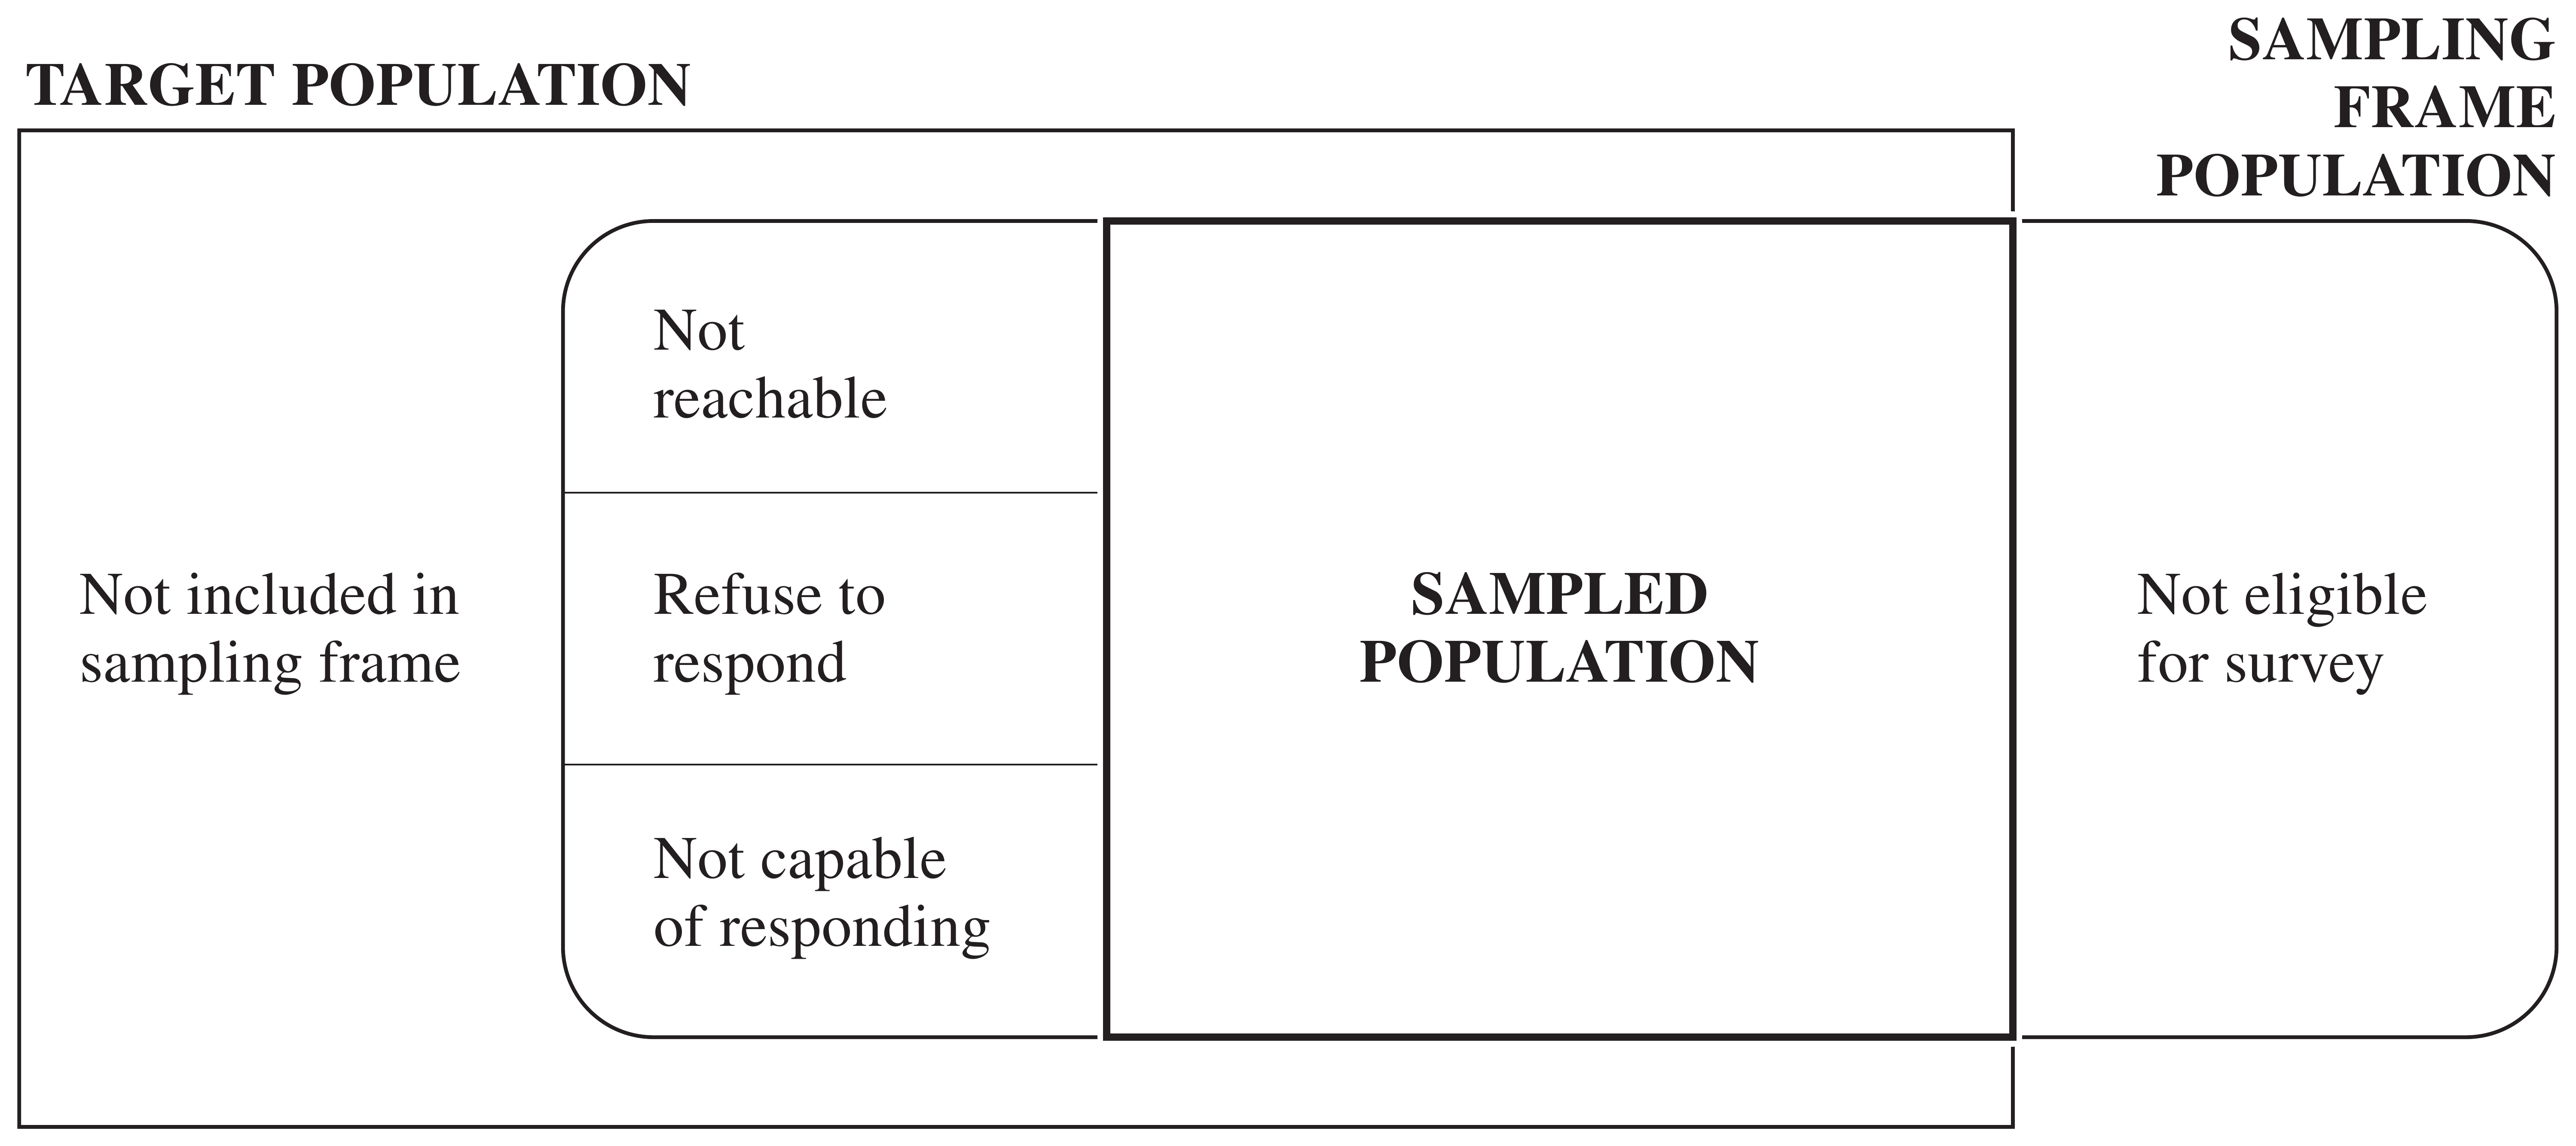
\includegraphics[width=0.9\linewidth,height=\textheight,keepaspectratio]{figures/target-sampled-population.png}

}

\caption{\label{fig-target-sampled}Target population, sampling frame
population and sampled population. The sampled population is only the
part of the target population that is in the frame and can and will
respond.}

\end{figure}%

In the Hite study the element was an individual woman and the target
population was all adult U.S. women. The sampled population, however,
was women who belonged to the organizations that received questionnaires
\emph{and} who would complete and return them.

\section{Selection Bias}\label{sec-intro-selection-bias}

\textbf{Selection bias} occurs when part of the target population is not
in the sampled population or, more generally, when some population units
are sampled at a different rate than intended by the investigator. A
\textbf{sample of convenience} is often biased, because the units that
are easiest to select, or most likely to respond, are usually not
representative of the harder-to-select or nonresponding units. For
example:

\begin{itemize}
\tightlist
\item
  A convenience sample of adolescents used to study communication about
  AIDS probably overestimated how much parents and teenagers talk about
  it. Adolescents willing to talk to investigators are also more likely
  to talk to other authority figures, such as their parents.
\item
  \textbf{Misspecifying the target population.} Polls before the 1994
  Arizona gubernatorial primary predicted that Eddie Basha would trail
  by 9 or more points; he won with 37\% of the vote. The polls targeted
  people who had voted in past primaries and missed the new rural voters
  who supported Basha.
\end{itemize}

Selection bias has several common sources.

\textbf{Undercoverage} is the failure to include all of the target
population in the sampling frame. The U.S. Behavioral Risk Factor
Surveillance System, a telephone survey, misses households without
telephones and for many years missed households with only cell phones.
Coverage varies by region and by income, so undercoverage can bias the
estimates.

\textbf{Overcoverage} is the inclusion in the sampling frame of units
that are not in the target population, for example when interviewers
include respondents under 18 in a radio survey meant for adults only.

\textbf{Nonresponse} is the failure to obtain responses from all of the
units chosen for the sample. It distorts the results even when the other
sources of selection bias are minimized. Nonrespondents often differ in
critical ways from respondents, but the extent of the difference is
usually unknown. Some published surveys have response rates as low as
10\%. It is difficult to generalize from such a survey when 90\% of the
sample could not be reached or refused to take part.

\section{Measurement Error}\label{sec-intro-measurement-error}

When a response differs from the true value, \textbf{measurement error}
has occurred. \textbf{Measurement bias} occurs when the responses tend
to differ from the truth in one direction. Like selection bias,
measurement bias must be considered and minimized at the design stage;
no amount of data analysis can remove it afterwards. Some sources of
measurement error:

\begin{itemize}
\tightlist
\item
  \textbf{People do not always tell the truth.} Farmers receiving food
  aid may underreport their crop yields, hoping to receive more aid.
\item
  \textbf{People do not always understand the questions.} A 1993 Roper
  poll found that 25\% of Americans did not believe the Holocaust had
  happened. The question used a confusing double negative. When it was
  reworded, only 1\% thought it ``possible'' that the Holocaust never
  happened.
\item
  \textbf{People forget.} In the U.S. National Crime Victimization
  Survey (NCVS), respondents asked about crimes in the last six months
  sometimes include events from further back. This is called
  \textbf{telescoping}.
\end{itemize}

Careful questionnaire design reduces measurement error:

\begin{itemize}
\tightlist
\item
  \textbf{Always test the questions} on a small group before the survey
  is carried out.
\item
  \textbf{Keep the questions simple and clear.} Belson (1981) tested the
  question ``What \emph{proportion} of your evening viewing time do you
  spend watching news programmes?'' on 53 people. Only 14 interpreted
  ``proportion'' correctly, as a percentage, part or fraction.
\item
  \textbf{Use specific questions instead of general ones.} Instead of
  asking ``Did anyone attack you in the last six months?'', the NCVS
  asks a detailed series of questions: ``With any weapon, for instance a
  gun or knife'', ``With anything like a baseball bat, frying pan,
  scissors, or stick'', and so on.
\end{itemize}

\section{Sampling and Nonsampling Errors}\label{sec-intro-errors}

\textbf{Sampling error} results from taking one sample instead of
examining the whole population. A different sample would likely give a
different result. Sampling error is what a poll's ``margin of error''
describes, and because it comes from the random selection of the sample,
it can be quantified in probabilistic terms. Most of this book is about
measuring and reducing it.

\textbf{Nonsampling errors}, such as selection bias and measurement
error, cannot be attributed to sample-to-sample variability. They are
often far larger than the sampling error. A survey may proudly report a
margin of error of 3\% based on a 30\% response rate, while ignoring the
large selection bias that such a response rate may cause.

\subsection{Why sample at all?}\label{why-sample-at-all}

If samples have errors, why not always take a census of the whole
population?

\begin{itemize}
\tightlist
\item
  \textbf{Cost.} A sample provides reliable information at far less cost
  than a census, and with a probability sample the sampling error can be
  quantified. Some measurements are destructive (for example,
  pulverizing a cookie to measure its fat content), so a census is not
  even possible.
\item
  \textbf{Speed.} Data from a sample can be collected and processed more
  quickly, so the estimates are timely. An unemployment rate for 2005
  published in 2015 would be useless.
\item
  \textbf{Accuracy.} Estimates from a sample can be \emph{more} accurate
  than those from a census. A census requires a large administrative
  effort with many data collectors, while a smaller operation allows the
  investigators to be more careful and to reduce nonsampling errors.
\end{itemize}

\section{Overview of Probability Sampling and Estimation
Techniques}\label{sec-intro-designs}

In a \textbf{probability sample}, every unit in the population has a
known, positive chance of being selected, and the sample is chosen by a
random mechanism. This removes selection bias due to the investigator's
choices, and it makes it possible to quantify the sampling error. This
section previews the techniques studied in the rest of the book: three
basic designs for drawing the sample (simple random, stratified and
cluster sampling), estimators that use auxiliary information (ratio and
regression estimation), and designs with unequal selection
probabilities. Each has its own chapter later in the book.

To compare the designs we use synthetic populations of \(N = 1000\)
units, with the \(y\)-values drawn from exponential distributions. The
population for SRS and stratified sampling (Figure~\ref{fig-intro-srs}
and Figure~\ref{fig-intro-stratified}) consists of four strata of sizes
400, 300, 200 and 100 whose means differ a lot: each is an exponential
distribution with mean 1.5, shifted by 0, 4, 8 and 12 respectively. The
population for cluster sampling (Figure~\ref{fig-intro-cluster})
consists of ten clusters whose sizes range from 40 to 160 units,
exponential with means from 2 to 8. Each design selects \(n = 60\)
units, shown in red; the unselected units are grey.

\textbf{Simple random sampling.} A \textbf{simple random sample (SRS)}
is the simplest probability sample. An SRS of size \(n\) is taken when
every possible subset of \(n\) units in the population has the same
chance of being the sample. The design uses no information about the
groups: in Figure~\ref{fig-intro-srs} the 1000 units are listed in an
arbitrary order, and 60 of them are chosen at random. By chance, a group
may be over- or under-represented, and the sample values range over the
whole spread of the population.

\begin{figure}

\centering{

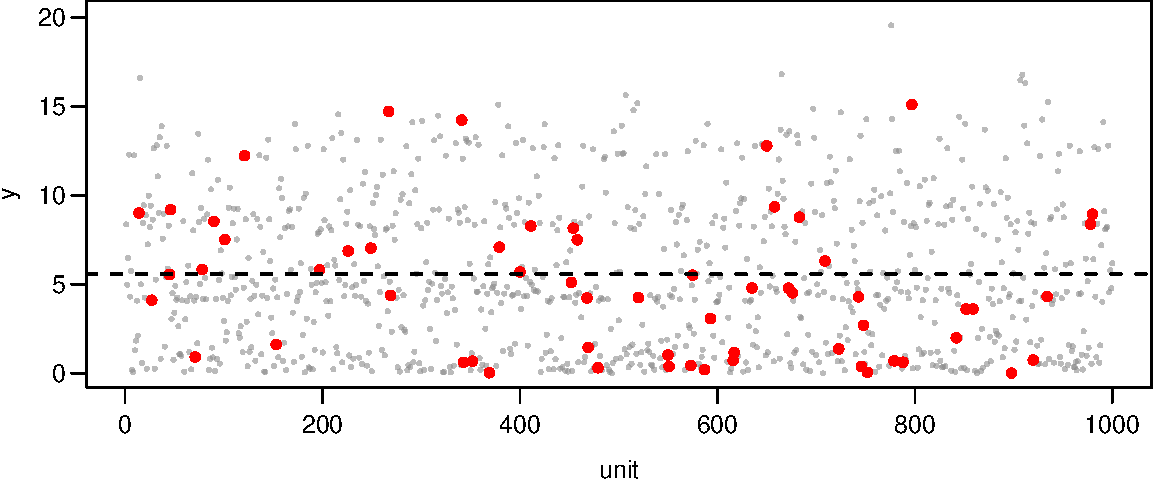
\includegraphics[width=0.85\linewidth,height=\textheight,keepaspectratio]{intro_files/figure-pdf/fig-intro-srs-1.pdf}

}

\caption{\label{fig-intro-srs}A simple random sample of \(n = 60\) (red)
from a population of \(N = 1000\) units, listed in an arbitrary order.
The dashed line is the population mean.}

\end{figure}%

\textbf{Stratified random sampling.} In a \textbf{stratified random
sample}, the population is divided into subgroups called
\textbf{strata}, and an SRS is selected independently from each stratum.
Strata are often subgroups of interest, such as provinces, terrain types
or firm sizes. In Figure~\ref{fig-intro-stratified} the same 1000 units
are arranged by stratum, with the strata sorted by their means (dashed
lines). The sample is allocated in proportion to the stratum sizes,
\(60 \times N_h/1000\), so 24, 18, 12 and 6 units are drawn from the
four strata. Every stratum is represented in the sample in a fixed
proportion. Stratification often increases precision, because units
within a stratum tend to be more similar than units selected at random
from the whole population. Here the stratum means are far apart while
the spread within each stratum is small, so the differences between the
strata, which make up most of the variation in
Figure~\ref{fig-intro-srs}, no longer contribute to the sampling error.

\begin{figure}

\centering{

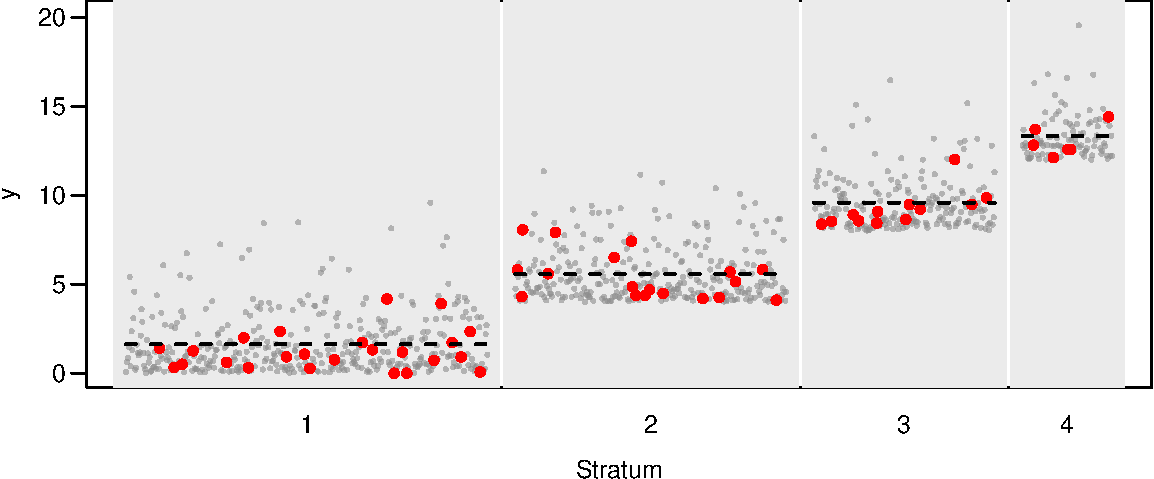
\includegraphics[width=0.85\linewidth,height=\textheight,keepaspectratio]{intro_files/figure-pdf/fig-intro-stratified-1.pdf}

}

\caption{\label{fig-intro-stratified}A stratified random sample from the
same population: the four strata are sorted by their means (dashed
lines), and SRSs of 24, 18, 12 and 6 units (red) are drawn from the
strata of sizes 400, 300, 200 and 100.}

\end{figure}%

\textbf{Cluster sampling.} In a \textbf{cluster sample}, the observation
units are grouped into larger sampling units called \textbf{clusters}.
For example, to survey Lutheran church members in Minneapolis without a
list of all members, we could take an SRS of churches (the clusters) and
then subsample members within each selected church (the observation
units). In Figure~\ref{fig-intro-cluster} the population consists of ten
clusters of different sizes, from 40 to 160 units, sorted by their
means. Three clusters are selected at random (shaded), and 20 units are
subsampled in each. This is convenient, since only three clusters need
to be visited, but the seven clusters that are not selected contribute
nothing to the sample. When the cluster means differ, the estimate
depends heavily on \emph{which} clusters happen to be chosen. Members of
the same church may likewise be more similar to each other than a random
sample of Lutherans would be. A cluster sample therefore often provides
less information than an SRS of the same size, and the gain in
convenience must be weighed against the loss in precision.

\begin{figure}

\centering{

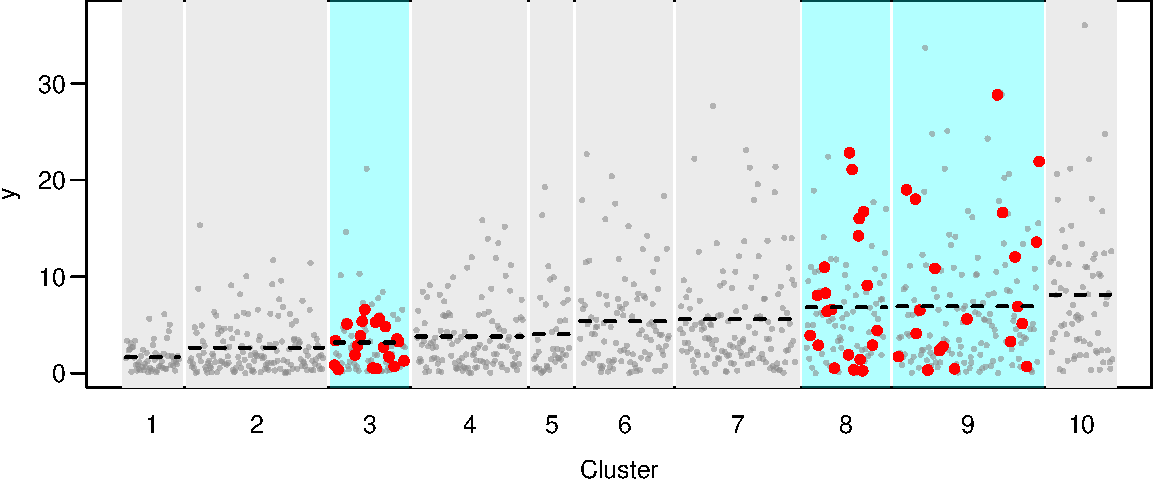
\includegraphics[width=0.85\linewidth,height=\textheight,keepaspectratio]{intro_files/figure-pdf/fig-intro-cluster-1.pdf}

}

\caption{\label{fig-intro-cluster}A cluster sample from a population of
ten clusters of 40 to 160 units, sorted by their means (dashed lines).
Three clusters are selected at random (shaded), and 20 units (red) are
subsampled in each; the other clusters are not observed at all.}

\end{figure}%

\textbf{Using auxiliary information: ratio and regression estimation.}
Often we know, for every unit in the population, an \textbf{auxiliary
variable} \(x_i\) that is related to \(y_i\): last year's value of
\(y\), the size of a farm, the floor area of a store. Ratio and
regression estimation take an ordinary sample but use the known \(x_i\)
at the \emph{estimation} stage. In Figure~\ref{fig-intro-ratio}, \(y\)
is roughly proportional to \(x\). From an SRS (green circles) we
estimate the slope \(\hat B = \bar y/\bar x\) of the line \(y = Bx\)
(red), and use it to predict \(y\) for every unit of the population from
its known \(x_i\) (red points). The \textbf{ratio estimate}
\(\hat{\bar y}_r = \hat B\,\bar x_U\) is the average of these
predictions. In this sample the green units happen to have large \(x\),
so the sample mean \(\bar y\) is too high. The ratio estimate corrects
for this through the known \(\bar x_U\) and lands close to \(\bar y_U\).
\textbf{Regression estimation} does the same with a fitted line
\(y = B_0 + B_1x\) that need not pass through the origin. Both are
studied in Section~\ref{sec-ratio-formulas} and the sections that
follow.

\begin{figure}

\centering{

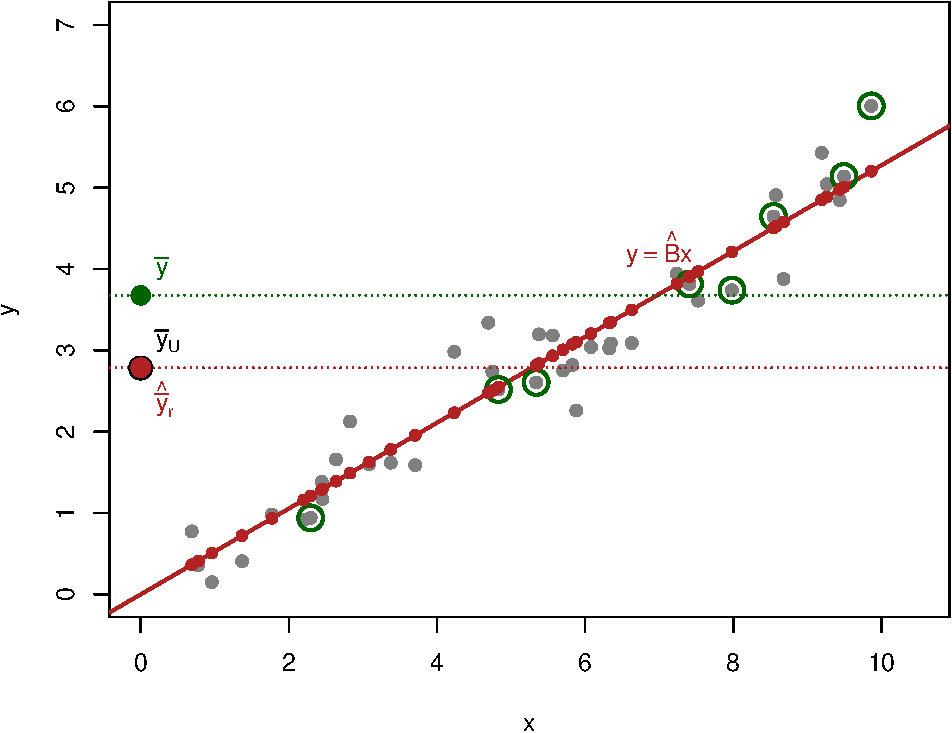
\includegraphics[width=0.65\linewidth,height=\textheight,keepaspectratio]{intro_files/figure-pdf/fig-intro-ratio-1.pdf}

}

\caption{\label{fig-intro-ratio}Ratio estimation. Grey: the population,
whose \(x_i\) are all known. Green circles: an SRS. Red: the line
\(y = \hat B x\) fitted from the sample and the predicted value
\(\hat B x_i\) of every unit. Left margin: the population mean
\(\bar y_U\) (black), the sample mean \(\bar y\) (green) and the ratio
estimate \(\hat{\bar y}_r\), the mean of the red points.}

\end{figure}%

\textbf{Unequal probability sampling.} Auxiliary information can also be
used at the \emph{design} stage. In \textbf{unequal probability sampling
(UPS)}, units are selected with different probabilities, usually
proportional to a measure of size \(x_i\) that is expected to be roughly
proportional to \(y_i\). Large units, which contribute most to the
population total, are then more likely to be in the sample. In
Figure~\ref{fig-intro-ups} the units of Figure~\ref{fig-intro-srs} are
drawn again, each with a size measure \(x_i\) equal to \(y_i\)
multiplied by a random error, and the point sizes show the inclusion
probabilities \(\pi_i \propto x_i\). A sample of 60 units (red) is drawn
with these probabilities. Most of the sampled units have large \(y\), so
the plain sample mean would be far too high. Each unit must instead be
weighted by its sampling weight \(w_i = 1/\pi_i\)
(Section~\ref{sec-intro-framework}), which gives the many small units
their due. When \(x_i\) is nearly proportional to \(y_i\), the weighted
estimator \(\sum_{i\in\mathcal S} y_i/\pi_i\) of the total is very
precise, because \(y_i/\pi_i\) is nearly the same for every unit. UPS is
studied in Section~\ref{sec-ups-hh} and the sections that follow.

\begin{figure}

\centering{

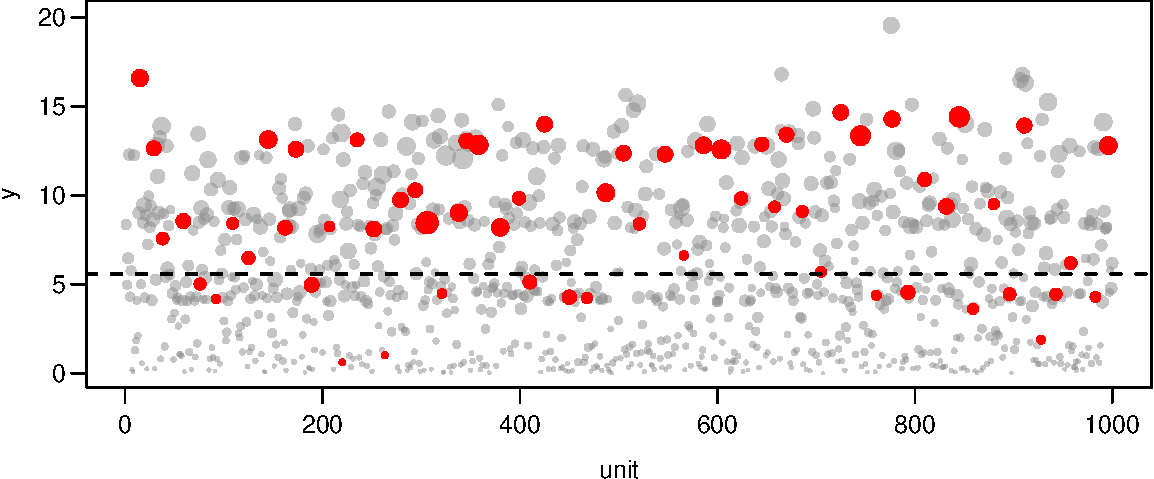
\includegraphics[width=0.85\linewidth,height=\textheight,keepaspectratio]{intro_files/figure-pdf/fig-intro-ups-1.pdf}

}

\caption{\label{fig-intro-ups}Unequal probability sampling from the
population of Figure~\ref{fig-intro-srs}. Each unit's inclusion
probability is proportional to a size measure \(x_i\) equal to \(y_i\)
times a random error; point sizes show the probabilities. The \(n = 60\)
sampled units (red) are mostly large ones. The dashed line is the
population mean.}

\end{figure}%

\section{A Framework for Probability
Sampling}\label{sec-intro-framework}

We now make the idea of a probability sample precise. The key concepts
are the population, the sample, the probabilities of the samples, the
inclusion probabilities, and the bias, variance and mean squared error
of an estimator.

\subsection{The population and its
samples}\label{the-population-and-its-samples}

The finite \textbf{population}, or \textbf{universe}, of \(N\) units is
denoted by the index set \[
\mathcal{U} = \{1, 2, \ldots, N\}.
\] Out of this population we can choose various \textbf{samples}, which
are subsets of \(\mathcal{U}\). The sample actually chosen is denoted
\(\mathcal{S}\); it consists of \(n\) of the units in \(\mathcal U\).

For example, suppose \(\mathcal{U} = \{1,2,3,4\}\), so \(N=4\). There
are \(\binom42 = 6\) different samples of size \(n=2\): \[
\mathcal{S}_1=\{1,2\},\quad \mathcal{S}_2=\{1,3\},\quad \mathcal{S}_3=\{1,4\},\quad
\mathcal{S}_4=\{2,3\},\quad \mathcal{S}_5=\{2,4\},\quad \mathcal{S}_6=\{3,4\}.
\]

\subsection{Probability sampling}\label{probability-sampling}

In \textbf{probability sampling}, each possible sample \(\mathcal{S}\)
has a known probability \(P(\mathcal{S})\) of being chosen, and the
probabilities of all possible samples sum to 1. The collection of these
probabilities is the \textbf{sampling design}. One possible design for a
sample of size 2 from \(\mathcal{U}=\{1,2,3,4\}\) is \[
P(\mathcal{S}_1)=\tfrac13,\quad P(\mathcal{S}_4)=\tfrac16,\quad P(\mathcal{S}_6)=\tfrac12,
\quad P(\mathcal{S}_2)=P(\mathcal{S}_3)=P(\mathcal{S}_5)=0 .
\] The probabilities are known \textbf{before} the sample is drawn. One
way to carry out this design is to put six balls in a box, two labeled
1, one labeled 4 and three labeled 6, draw one ball at random, and take
the sample \(\mathcal S_i\) whose label is drawn. An SRS is the special
design in which all six samples have probability \(1/6\).

\subsection{\texorpdfstring{The values
\(y_i\)}{The values y\_i}}\label{the-values-y_i}

Let \(y_i\) be a characteristic of the \(i\)th unit in the population,
such as the corn yield of farm \(i\):

{\def\LTcaptype{none} % do not increment counter
\begin{longtable}[]{@{}cccccc@{}}
\toprule\noalign{}
\(i\) & 1 & 2 & 3 & \(\cdots\) & \(N\) \\
\midrule\noalign{}
\endhead
\bottomrule\noalign{}
\endlastfoot
\(y_i\) & \(y_1\) & \(y_2\) & \(y_3\) & \(\cdots\) & \(y_N\) \\
\end{longtable}
}

We treat each \(y_i\) as a \textbf{fixed} quantity. If farm 723 is in
the sample, its corn yield \(y_{723}\) is known exactly; if it is not,
\(y_{723}\) is unknown but still fixed. The only randomness is in
\emph{which} units are selected. This is the \textbf{design-based} (or
randomization) approach, followed by Lohr and by this book. (Scheaffer
et al.~use \(Y_i\) for a random variable and \(y_i\) for its value.)

\subsection{Inclusion probabilities and sampling
weights}\label{inclusion-probabilities-and-sampling-weights}

Once a sampling design is chosen, each unit in the population has a
known probability of appearing in the sample, its \textbf{inclusion
probability} \begin{equation}\protect\phantomsection\label{eq-include}{
\pi_i = P(\text{unit } i \text{ is in the sample}) = \sum_{\mathcal S \ni i} P(\mathcal S),
}\end{equation} the sum of the probabilities of all possible samples
that contain unit \(i\). In probability sampling all the \(\pi_i\) are
known before the survey starts, and we assume \(\pi_i > 0\) for every
unit, so that every unit has a chance to be observed.

For the design above, unit 1 belongs only to \(\mathcal S_1 = \{1,2\}\)
among the samples with positive probability, so \[
\pi_1 = P(\{1,2\}) = \tfrac13, \qquad
\pi_2 = P(\{1,2\})+P(\{2,3\}) = \tfrac13+\tfrac16=\tfrac12,
\] \[
\pi_3 = P(\{2,3\})+P(\{3,4\}) = \tfrac16+\tfrac12=\tfrac23, \qquad
\pi_4 = P(\{3,4\}) = \tfrac12 .
\] The inclusion probabilities do not sum to 1. They sum to 2, because
every sample contains \(n = 2\) units; in general
\(\sum_{i=1}^N \pi_i = n\) for a design with fixed sample size \(n\).

The \textbf{sampling weight} of unit \(i\) is \(w_i = 1/\pi_i\). It can
be thought of as the number of population units that a sampled unit
represents. For many sampling designs, the estimator of the population
total can be written as \[
\hat t = \sum_{i \in \mathcal{S}} w_i \, y_i = \sum_{i \in \mathcal{S}} \frac{y_i}{\pi_i}.
\] For an SRS, \(\pi_i = n/N\) and \(w_i = N/n\) for every unit; for the
other designs in this book, the weights differ between units.

\subsection{Population quantities}\label{population-quantities}

The quantities we want to estimate are characteristics of the fixed
values \(y_1, \ldots, y_N\): \[
\textbf{total: } t = \sum_{i=1}^N y_i, \qquad
\textbf{mean: } \bar y_{U} = \frac{t}{N},
\] \[
\textbf{variance: } S^2 = \frac{1}{N-1}\sum_{i=1}^N (y_i-\bar y_{U})^2, \qquad
\textbf{standard deviation: } S = \sqrt{S^2}.
\] Scheaffer et al.~instead use
\(\sigma^2 = \frac1N \sum_{i=1}^N (y_i - \bar y_{U})^2\), dividing by
\(N\) rather than \(N-1\). The two differ only by the factor
\((N-1)/N\).

\textbf{Example: a population proportion.} Let \(y_i = 1\) if unit \(i\)
has some attribute and \(y_i = 0\) otherwise:

{\def\LTcaptype{none} % do not increment counter
\begin{longtable}[]{@{}cccccc@{}}
\toprule\noalign{}
\(i\) & 1 & 2 & 3 & 4 & 5 \\
\midrule\noalign{}
\endhead
\bottomrule\noalign{}
\endlastfoot
\(y_i\) & 1 & 0 & 0 & 0 & 1 \\
\end{longtable}
}

Then the total is the number of units with the attribute and the mean is
the population proportion: \[
t = 1+0+0+0+1 = 2, \qquad
\bar y_{U} = \frac{2}{5} = 0.4,
\] \[
S^2 = \frac{1}{5-1}\Big((1-0.4)^2\times 2 + (0-0.4)^2\times 3\Big) = 0.3 .
\] For a 0/1 variable, \(S^2 = \frac{N}{N-1}\,p(1-p)\) with
\(p = \bar y_U\); here \(\frac54(0.4)(0.6) = 0.3\). As \(N\) grows,
\(S^2 \to p(1-p)\).

\textbf{Example: number of devices per household.} A population of
\(N = 4\) households has the following numbers of devices:

{\def\LTcaptype{none} % do not increment counter
\begin{longtable}[]{@{}ccccc@{}}
\toprule\noalign{}
\(i\) & 1 & 2 & 3 & 4 \\
\midrule\noalign{}
\endhead
\bottomrule\noalign{}
\endlastfoot
\(y_i\) & 2 & 4 & 4 & 6 \\
\end{longtable}
}

\[
t = 2+4+4+6 = 16, \qquad
\bar y_{U} = \frac{16}{4} = 4,
\] \[
S^2 = \frac{(2-4)^2+(4-4)^2+(4-4)^2+(6-4)^2}{4-1} = \frac{8}{3}.
\]

\subsection{Statistics and sampling
distributions}\label{statistics-and-sampling-distributions}

A \textbf{statistic} is a function of the observations in the sample,
used to estimate a population quantity. Since the sample is random, so
is the statistic. Its \textbf{sampling distribution} is its distribution
under repeated sampling: the values it takes over all possible samples,
with the probabilities \(P(\mathcal S)\) of those samples.

For example, to estimate the total \(t\) we may use the sample mean
scaled up by the population size, \[
\bar y = \frac{1}{n}\sum_{i\in\mathcal{S}} y_i, \qquad \hat t = N\bar y .
\] Take the devices population (\(\bar y_U = 4\), \(t = 16\)) with the
sampling design of the previous sections. For each of the six possible
samples of size 2 we can compute \(\bar y\):

{\def\LTcaptype{none} % do not increment counter
\begin{longtable}[]{@{}
  >{\centering\arraybackslash}p{(\linewidth - 12\tabcolsep) * \real{0.1429}}
  >{\centering\arraybackslash}p{(\linewidth - 12\tabcolsep) * \real{0.1429}}
  >{\centering\arraybackslash}p{(\linewidth - 12\tabcolsep) * \real{0.1429}}
  >{\centering\arraybackslash}p{(\linewidth - 12\tabcolsep) * \real{0.1429}}
  >{\centering\arraybackslash}p{(\linewidth - 12\tabcolsep) * \real{0.1429}}
  >{\centering\arraybackslash}p{(\linewidth - 12\tabcolsep) * \real{0.1429}}
  >{\centering\arraybackslash}p{(\linewidth - 12\tabcolsep) * \real{0.1429}}@{}}
\toprule\noalign{}
\begin{minipage}[b]{\linewidth}\centering
\(\mathcal S\)
\end{minipage} & \begin{minipage}[b]{\linewidth}\centering
\(\{1,2\}\)
\end{minipage} & \begin{minipage}[b]{\linewidth}\centering
\(\{1,3\}\)
\end{minipage} & \begin{minipage}[b]{\linewidth}\centering
\(\{1,4\}\)
\end{minipage} & \begin{minipage}[b]{\linewidth}\centering
\(\{2,3\}\)
\end{minipage} & \begin{minipage}[b]{\linewidth}\centering
\(\{2,4\}\)
\end{minipage} & \begin{minipage}[b]{\linewidth}\centering
\(\{3,4\}\)
\end{minipage} \\
\midrule\noalign{}
\endhead
\bottomrule\noalign{}
\endlastfoot
values & 2, 4 & 2, 4 & 2, 6 & 4, 4 & 4, 6 & 4, 6 \\
\(P(\mathcal S)\) & \(1/3\) & \(0\) & \(0\) & \(1/6\) & \(0\) &
\(1/2\) \\
\(\bar y\) & 3 & 3 & 4 & 4 & 5 & 5 \\
\end{longtable}
}

Collecting the samples that give the same value of \(\bar y\), and
adding their probabilities, gives the \textbf{sampling distribution of
\(\bar y\)} (Figure~\ref{fig-intro-sampdist}):

{\def\LTcaptype{none} % do not increment counter
\begin{longtable}[]{@{}cccc@{}}
\toprule\noalign{}
\(k\) & 3 & 4 & 5 \\
\midrule\noalign{}
\endhead
\bottomrule\noalign{}
\endlastfoot
\(P(\bar y = k)\) & \(1/3\) & \(1/6\) & \(1/2\) \\
\end{longtable}
}

\begin{figure}

\centering{

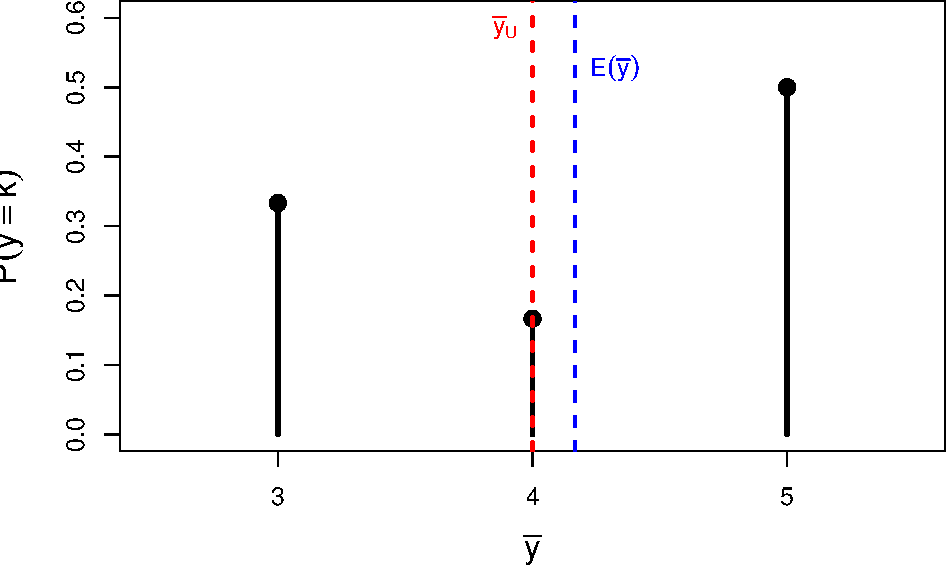
\includegraphics[width=0.7\linewidth,height=\textheight,keepaspectratio]{intro_files/figure-pdf/fig-intro-sampdist-1.pdf}

}

\caption{\label{fig-intro-sampdist}Sampling distribution of \(\bar y\)
for the devices population under the design \(P(\{1,2\}) = 1/3\),
\(P(\{2,3\}) = 1/6\), \(P(\{3,4\}) = 1/2\). The mean of the
distribution, \(E(\bar y) = 25/6\), is not the population mean
\(\bar y_U = 4\).}

\end{figure}%

\subsection{Bias, variance and mean squared
error}\label{bias-variance-and-mean-squared-error}

The sampling distribution tells us how good an estimator \(\hat\theta\)
of a population quantity \(\theta\) is. Three summaries are used: \[
\text{Bias}(\hat\theta) = E(\hat\theta) - \theta, \qquad
V(\hat\theta) = E\big[(\hat\theta - E(\hat\theta))^2\big], \qquad
\text{MSE}(\hat\theta) = E\big[(\hat\theta - \theta)^2\big].
\] The variance measures the spread of the estimates around their own
mean; the MSE measures their spread around the true value.

For \(\bar y\) in the example, \[
E(\bar y) = 3\times\tfrac13 + 4\times\tfrac16 + 5\times\tfrac12 = \frac{25}{6},
\qquad
\text{Bias}(\bar y) = \frac{25}{6} - 4 = \frac16 ,
\] \[
V(\bar y) = \Big(3-\tfrac{25}{6}\Big)^2\tfrac13 + \Big(4-\tfrac{25}{6}\Big)^2\tfrac16
   + \Big(5-\tfrac{25}{6}\Big)^2\tfrac12 = \frac{29}{36} \approx 0.8056,
\] \[
\text{MSE}(\bar y) = (3-4)^2\cdot\tfrac13 + (4-4)^2\cdot\tfrac16 + (5-4)^2\cdot\tfrac12 = \frac56 \approx 0.8333 .
\] The estimator is biased under this design. The design favours the
sample \(\{3,4\}\), which contains the household with 6 devices, so
\(\bar y\) tends to be too large. Correspondingly \(\hat t = 4\bar y\)
has \(E(\hat t) = 50/3 \approx 16.67\), a bias of \(2/3\) for
\(t = 16\).

\textbf{MSE = Bias² + Variance.} Adding and subtracting
\(E(\hat\theta)\), \[
\text{MSE}(\hat\theta)
 = E\Big[\big(\hat\theta - E(\hat\theta)\big) + \big(E(\hat\theta) - \theta\big)\Big]^2
 = V(\hat\theta) + \big(\text{Bias}(\hat\theta)\big)^2 ,
\] because the cross term
\(2\,\text{Bias}(\hat\theta)\,E\big[\hat\theta - E(\hat\theta)\big]\) is
zero. In the example, \((1/6)^2 + 29/36 = 1/36 + 29/36 = 30/36 = 5/6\),
which agrees with the direct calculation. In particular, when
\(\hat\theta\) is unbiased, \(\text{MSE}(\hat\theta) = V(\hat\theta)\).

\textbf{The same population under SRS.} If instead all six samples have
probability \(1/6\) (an SRS), the six values of \(\bar y\) are
\(3, 3, 4, 4, 5, 5\), so \(E(\bar y) = 4 = \bar y_U\): the estimator is
now unbiased. Its variance is \(\frac16(1+1+0+0+1+1) = \frac23\), which
agrees with the SRS formula
\(\big(1-\frac nN\big)\frac{S^2}{n} = \frac12\cdot\frac{8/3}{2} = \frac23\)
of Section~\ref{sec-srs-formulas}. The short R enumeration below checks
both designs.

\begin{Shaded}
\begin{Highlighting}[]
\NormalTok{y }\OtherTok{\textless{}{-}} \FunctionTok{c}\NormalTok{(}\DecValTok{2}\NormalTok{, }\DecValTok{4}\NormalTok{, }\DecValTok{4}\NormalTok{, }\DecValTok{6}\NormalTok{)}
\NormalTok{samples }\OtherTok{\textless{}{-}} \FunctionTok{combn}\NormalTok{(}\DecValTok{4}\NormalTok{, }\DecValTok{2}\NormalTok{)                        }\CommentTok{\# the 6 possible samples, one per column}
\NormalTok{ybar }\OtherTok{\textless{}{-}} \FunctionTok{apply}\NormalTok{(samples, }\DecValTok{2}\NormalTok{, }\ControlFlowTok{function}\NormalTok{(s) }\FunctionTok{mean}\NormalTok{(y[s]))}
\NormalTok{designs }\OtherTok{\textless{}{-}} \FunctionTok{rbind}\NormalTok{(}\AttributeTok{unequal =} \FunctionTok{c}\NormalTok{(}\DecValTok{1}\SpecialCharTok{/}\DecValTok{3}\NormalTok{, }\DecValTok{0}\NormalTok{, }\DecValTok{0}\NormalTok{, }\DecValTok{1}\SpecialCharTok{/}\DecValTok{6}\NormalTok{, }\DecValTok{0}\NormalTok{, }\DecValTok{1}\SpecialCharTok{/}\DecValTok{2}\NormalTok{),}
                 \AttributeTok{SRS     =} \FunctionTok{rep}\NormalTok{(}\DecValTok{1}\SpecialCharTok{/}\DecValTok{6}\NormalTok{, }\DecValTok{6}\NormalTok{))}
\FunctionTok{round}\NormalTok{(}\FunctionTok{t}\NormalTok{(}\FunctionTok{apply}\NormalTok{(designs, }\DecValTok{1}\NormalTok{, }\ControlFlowTok{function}\NormalTok{(P) \{}
\NormalTok{  E }\OtherTok{\textless{}{-}} \FunctionTok{sum}\NormalTok{(P }\SpecialCharTok{*}\NormalTok{ ybar)}
  \FunctionTok{c}\NormalTok{(}\AttributeTok{E =}\NormalTok{ E, }\AttributeTok{Bias =}\NormalTok{ E }\SpecialCharTok{{-}} \FunctionTok{mean}\NormalTok{(y), }\AttributeTok{V =} \FunctionTok{sum}\NormalTok{(P }\SpecialCharTok{*}\NormalTok{ (ybar }\SpecialCharTok{{-}}\NormalTok{ E)}\SpecialCharTok{\^{}}\DecValTok{2}\NormalTok{), }\AttributeTok{MSE =} \FunctionTok{sum}\NormalTok{(P }\SpecialCharTok{*}\NormalTok{ (ybar }\SpecialCharTok{{-}} \FunctionTok{mean}\NormalTok{(y))}\SpecialCharTok{\^{}}\DecValTok{2}\NormalTok{))}
\NormalTok{\})), }\DecValTok{4}\NormalTok{)}
\end{Highlighting}
\end{Shaded}

\begin{verbatim}
             E   Bias      V    MSE
unequal 4.1667 0.1667 0.8056 0.8333
SRS     4.0000 0.0000 0.6667 0.6667
\end{verbatim}

\subsection{Unbiased, precise and
accurate}\label{unbiased-precise-and-accurate}

An estimator \(\hat t\) of \(t\) is

\begin{itemize}
\tightlist
\item
  \textbf{unbiased} if \(E(\hat t) = t\);
\item
  \textbf{precise} if \(V(\hat t) = E\big[(\hat t - E[\hat t])^2\big]\)
  is small;
\item
  \textbf{accurate} if
  \(\text{MSE}(\hat t) = E\big[(\hat t - t)^2\big]\) is small.
\end{itemize}

Precision measures how close the estimates from different samples are to
\emph{each other}; accuracy measures how close they are to the
\emph{truth}. A badly biased estimator may be very precise but will not
be accurate. Figure~\ref{fig-archers} shows the three cases as archers
aiming at the centre of a target: archer A is unbiased but imprecise,
archer B is precise but biased, and archer C is both unbiased and
precise, and therefore accurate. Selection bias and measurement bias
make a survey like archer B: increasing the sample size makes the
estimates more precise, but no closer to the truth.

\begin{figure}

\centering{

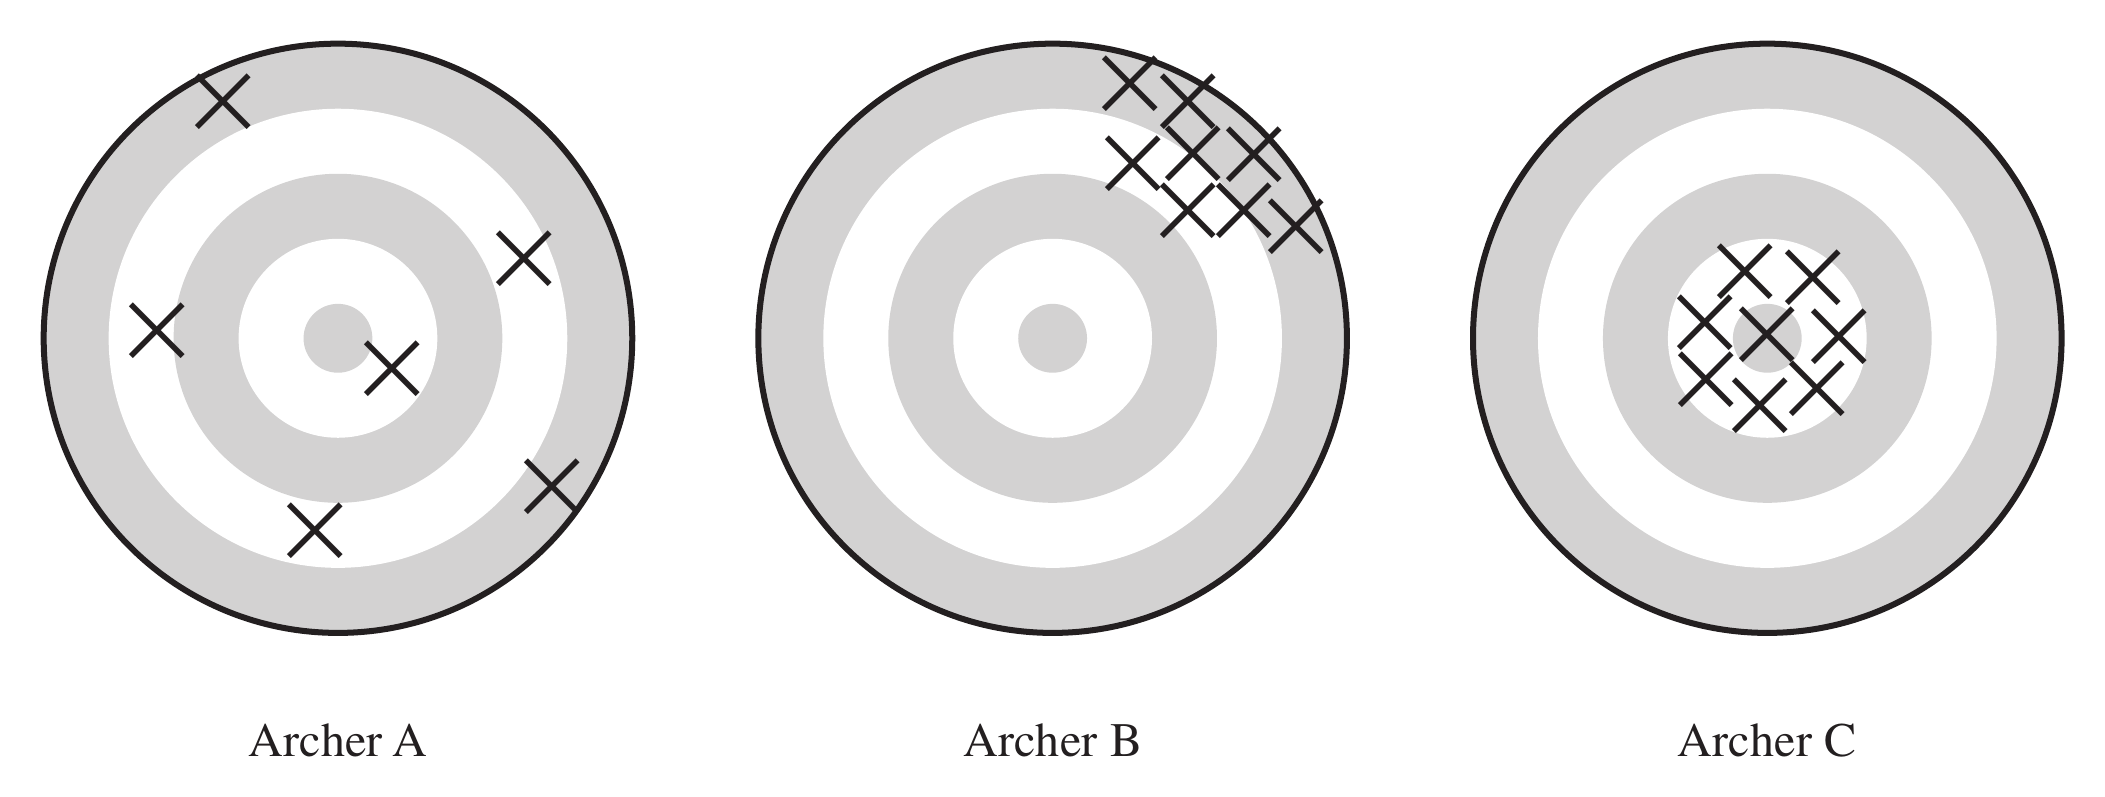
\includegraphics[width=0.95\linewidth,height=\textheight,keepaspectratio]{figures/archers.png}

}

\caption{\label{fig-archers}Unbiased but imprecise (A), precise but
biased (B), and accurate (C).}

\end{figure}%

\subsection{Summary}\label{summary}

The finite population \(\mathcal U\) consists of the units
\(\{1,2,\ldots,N\}\), with values \(\{y_1,y_2,\ldots,y_N\}\). We select
a sample \(\mathcal S\) of \(n\) units from \(\mathcal U\) using the
selection probabilities that define the sampling design. The \(y_i\) are
fixed but unknown quantities, unknown unless unit \(i\) happens to
appear in the sample. All statements about the bias, variance and MSE of
an estimator refer to its distribution over the possible samples. The
following chapters work out these properties for each design, starting
with simple random sampling in Section~\ref{sec-srs-design}.

\bookmarksetup{startatroot}

\chapter{Data Analysis with R}\label{data-analysis-with-r}

Modern workflows with the native pipe, dplyr, gt, and ggplot2

\hfill\break

\begin{Shaded}
\begin{Highlighting}[]
\FunctionTok{library}\NormalTok{(dplyr)}
\FunctionTok{library}\NormalTok{(gt)}
\FunctionTok{library}\NormalTok{(gtsummary)}
\FunctionTok{library}\NormalTok{(ggplot2)}
\end{Highlighting}
\end{Shaded}

All packages are loaded once in a hidden \texttt{setup} chunk, and
\texttt{message}/\texttt{warning} suppression is set globally in the
YAML header rather than repeated on every chunk.

\section{Foundations}\label{foundations}

\subsection{Basic R objects}\label{basic-r-objects}

\begin{Shaded}
\begin{Highlighting}[]
\CommentTok{\# vectors}
\NormalTok{x }\OtherTok{\textless{}{-}} \FunctionTok{seq}\NormalTok{(}\DecValTok{30}\NormalTok{, }\DecValTok{3}\NormalTok{, }\AttributeTok{by =} \SpecialCharTok{{-}}\DecValTok{2}\NormalTok{)}
\NormalTok{a }\OtherTok{\textless{}{-}} \FunctionTok{c}\NormalTok{(}\FloatTok{66.32}\NormalTok{, }\FloatTok{69.87}\NormalTok{, }\FloatTok{70.12}\NormalTok{, }\FloatTok{90.37}\NormalTok{, }\FloatTok{50.08}\NormalTok{, }\FloatTok{61.20}\NormalTok{, }\FloatTok{65.00}\NormalTok{, }\FloatTok{57.65}\NormalTok{)}

\NormalTok{a[}\DecValTok{1}\NormalTok{]            }\CommentTok{\# extract an element}
\end{Highlighting}
\end{Shaded}

\begin{verbatim}
[1] 66.32
\end{verbatim}

\begin{Shaded}
\begin{Highlighting}[]
\NormalTok{a[}\DecValTok{1}\NormalTok{] }\OtherTok{\textless{}{-}} \FloatTok{85.34}   \CommentTok{\# replace an element}
\NormalTok{ma }\OtherTok{\textless{}{-}} \FunctionTok{mean}\NormalTok{(a)}
\NormalTok{ma}
\end{Highlighting}
\end{Shaded}

\begin{verbatim}
[1] 68.70375
\end{verbatim}

\begin{Shaded}
\begin{Highlighting}[]
\CommentTok{\# read a vector of numbers from text without saving a file first}
\NormalTok{y }\OtherTok{\textless{}{-}} \FunctionTok{scan}\NormalTok{(}\AttributeTok{text =} \StringTok{"7 8 9 10 11 12 13 13 14 17 17 45"}\NormalTok{)}
\NormalTok{y}
\end{Highlighting}
\end{Shaded}

\begin{verbatim}
 [1]  7  8  9 10 11 12 13 13 14 17 17 45
\end{verbatim}

\begin{Shaded}
\begin{Highlighting}[]
\CommentTok{\# matrices: matrix() fills by column unless byrow = TRUE}
\NormalTok{A }\OtherTok{\textless{}{-}} \FunctionTok{matrix}\NormalTok{(}\DecValTok{1}\SpecialCharTok{:}\DecValTok{8}\NormalTok{, }\AttributeTok{nrow =} \DecValTok{4}\NormalTok{, }\AttributeTok{ncol =} \DecValTok{2}\NormalTok{)}
\NormalTok{A}
\end{Highlighting}
\end{Shaded}

\begin{verbatim}
     [,1] [,2]
[1,]    1    5
[2,]    2    6
[3,]    3    7
[4,]    4    8
\end{verbatim}

\begin{Shaded}
\begin{Highlighting}[]
\NormalTok{D }\OtherTok{\textless{}{-}} \FunctionTok{matrix}\NormalTok{(a, }\AttributeTok{nrow =} \DecValTok{4}\NormalTok{, }\AttributeTok{ncol =} \DecValTok{2}\NormalTok{, }\AttributeTok{byrow =} \ConstantTok{TRUE}\NormalTok{)}
\NormalTok{D}
\end{Highlighting}
\end{Shaded}

\begin{verbatim}
      [,1]  [,2]
[1,] 85.34 69.87
[2,] 70.12 90.37
[3,] 50.08 61.20
[4,] 65.00 57.65
\end{verbatim}

\begin{Shaded}
\begin{Highlighting}[]
\CommentTok{\# a larger matrix, to illustrate element and row assignment}
\NormalTok{B }\OtherTok{\textless{}{-}} \FunctionTok{matrix}\NormalTok{(}\DecValTok{1}\SpecialCharTok{:}\DecValTok{5000}\NormalTok{, }\AttributeTok{nrow =} \DecValTok{100}\NormalTok{, }\AttributeTok{ncol =} \DecValTok{50}\NormalTok{)}
\NormalTok{B[}\DecValTok{2}\NormalTok{, }\DecValTok{4}\NormalTok{] }\OtherTok{\textless{}{-}} \DecValTok{45}
\NormalTok{B[}\DecValTok{1}\NormalTok{, ] }\OtherTok{\textless{}{-}} \DecValTok{1}\SpecialCharTok{:}\DecValTok{50}
\FunctionTok{head}\NormalTok{(B[}\DecValTok{1}\NormalTok{, ])   }\CommentTok{\# part of the first row}
\end{Highlighting}
\end{Shaded}

\begin{verbatim}
[1] 1 2 3 4 5 6
\end{verbatim}

\begin{Shaded}
\begin{Highlighting}[]
\FunctionTok{head}\NormalTok{(B[, }\DecValTok{1}\NormalTok{])   }\CommentTok{\# part of the first column}
\end{Highlighting}
\end{Shaded}

\begin{verbatim}
[1] 1 2 3 4 5 6
\end{verbatim}

\begin{Shaded}
\begin{Highlighting}[]
\CommentTok{\# lists}
\NormalTok{E }\OtherTok{\textless{}{-}} \FunctionTok{list}\NormalTok{(}\AttributeTok{newa =}\NormalTok{ a, }\AttributeTok{newA =}\NormalTok{ A)}
\FunctionTok{names}\NormalTok{(E)}
\end{Highlighting}
\end{Shaded}

\begin{verbatim}
[1] "newa" "newA"
\end{verbatim}

\begin{Shaded}
\begin{Highlighting}[]
\NormalTok{E}\SpecialCharTok{$}\NormalTok{newA}
\end{Highlighting}
\end{Shaded}

\begin{verbatim}
     [,1] [,2]
[1,]    1    5
[2,]    2    6
[3,]    3    7
[4,]    4    8
\end{verbatim}

\begin{Shaded}
\begin{Highlighting}[]
\NormalTok{E}\SpecialCharTok{$}\NormalTok{newa }\OtherTok{\textless{}{-}} \DecValTok{10}\SpecialCharTok{:}\DecValTok{17}

\CommentTok{\# data frames}
\NormalTok{stat245\_scores }\OtherTok{\textless{}{-}} \FunctionTok{data.frame}\NormalTok{(}
  \AttributeTok{student =} \FunctionTok{c}\NormalTok{(}\StringTok{"Peter"}\NormalTok{, }\StringTok{"John"}\NormalTok{, }\StringTok{"Alice"}\NormalTok{),}
  \AttributeTok{score   =} \FunctionTok{c}\NormalTok{(}\DecValTok{30}\NormalTok{, }\DecValTok{45}\NormalTok{, }\DecValTok{50}\NormalTok{)}
\NormalTok{)}
\NormalTok{stat245\_scores}
\end{Highlighting}
\end{Shaded}

\begin{verbatim}
  student score
1   Peter    30
2    John    45
3   Alice    50
\end{verbatim}

The column of names is called \texttt{student} rather than
\texttt{names}, so that the base function \texttt{names()} is not
masked.

\section{Importing a dataset}\label{importing-a-dataset}

\begin{Shaded}
\begin{Highlighting}[]
\NormalTok{data\_url }\OtherTok{\textless{}{-}} \StringTok{"https://raw.githubusercontent.com/longhaiSK/sampling/main/sampling\_book/data/"}
\NormalTok{agpop\_file }\OtherTok{\textless{}{-}} \FunctionTok{paste0}\NormalTok{(data\_url, }\StringTok{"agpop.csv"}\NormalTok{)}

\CommentTok{\# {-}99 is the missing{-}value code in this file, so convert it to NA on import}
\NormalTok{agpop }\OtherTok{\textless{}{-}} \FunctionTok{read.csv}\NormalTok{(agpop\_file, }\AttributeTok{na.strings =} \StringTok{"{-}99"}\NormalTok{)}

\FunctionTok{colnames}\NormalTok{(agpop)}
\end{Highlighting}
\end{Shaded}

\begin{verbatim}
 [1] "county"   "state"    "acres92"  "acres87"  "acres82"  "farms92"  "farms87"  "farms82"  "largef92"
[10] "largef87" "largef82" "smallf92" "smallf87" "smallf82" "region"  
\end{verbatim}

\begin{Shaded}
\begin{Highlighting}[]
\FunctionTok{c}\NormalTok{(}\AttributeTok{rows =} \FunctionTok{nrow}\NormalTok{(agpop), }\AttributeTok{cols =} \FunctionTok{ncol}\NormalTok{(agpop))}
\end{Highlighting}
\end{Shaded}

\begin{verbatim}
rows cols 
3078   15 
\end{verbatim}

Because \texttt{na.strings\ =\ "-99"} is applied at import, every
\texttt{-99} is already \texttt{NA} in \texttt{agpop}. All later
filtering therefore uses \texttt{is.na()}; comparisons such as
\texttt{acres92\ !=\ -99} no longer identify the missing values.

\subsection{Displaying the full
dataset}\label{displaying-the-full-dataset}

Printing several thousand rows into an HTML document consumes vertical
space and slows the browser. With \texttt{df-print:\ paged} (set under
\texttt{format:\ html} in the YAML header), a printed data frame appears
as a paged table: all rows are embedded as one lightweight data blob,
and only the current page is drawn. Static targets such as Typst or PDF
have no pager, so only the first rows are shown there.

\begin{Shaded}
\begin{Highlighting}[]
\FunctionTok{head}\NormalTok{(agpop)}
\end{Highlighting}
\end{Shaded}

\begin{verbatim}
                 county state acres92 acres87 acres82 farms92 farms87 farms82 largef92 largef87 largef82
1 ALEUTIAN ISLANDS AREA    AK  683533  726596  764514      26      27      28       14       16       20
2        ANCHORAGE AREA    AK   47146   59297  256709     217     245     223        9       10       11
3        FAIRBANKS AREA    AK  141338  154913  204568     168     175     170       25       28       21
4           JUNEAU AREA    AK     210     214     127       8       8      12        0        0        0
5  KENAI PENINSULA AREA    AK   50810   85712   98035      93     119     137        9       18       17
6        AUTAUGA COUNTY    AL  107259  116050  145044     322     388     453       25       32       32
  smallf92 smallf87 smallf82 region
1        6        4        1      W
2       41       52       38      W
3       12       18       25      W
4        5        4        8      W
5       12       18       19      W
6        8       19       17      S
\end{verbatim}

\subsection{Simple summaries}\label{simple-summaries}

\begin{Shaded}
\begin{Highlighting}[]
\FunctionTok{mean}\NormalTok{(agpop}\SpecialCharTok{$}\NormalTok{acres92, }\AttributeTok{na.rm =} \ConstantTok{TRUE}\NormalTok{)}
\end{Highlighting}
\end{Shaded}

\begin{verbatim}
[1] 308582.4
\end{verbatim}

\begin{Shaded}
\begin{Highlighting}[]
\FunctionTok{sd}\NormalTok{(agpop}\SpecialCharTok{$}\NormalTok{acres92, }\AttributeTok{na.rm =} \ConstantTok{TRUE}\NormalTok{)}
\end{Highlighting}
\end{Shaded}

\begin{verbatim}
[1] 425312.8
\end{verbatim}

\section{The native pipe}\label{the-native-pipe}

The native pipe \texttt{\textbar{}\textgreater{}} takes the value on its
left and passes it as the \textbf{first argument} to the function on its
right, so \texttt{x\ \textbar{}\textgreater{}\ f()} is another way of
writing \texttt{f(x)}. Pipes chain, so the output of one step feeds the
next.

\begin{Shaded}
\begin{Highlighting}[]
\NormalTok{x }\OtherTok{\textless{}{-}} \FunctionTok{c}\NormalTok{(}\DecValTok{1}\NormalTok{, }\DecValTok{2}\NormalTok{, }\DecValTok{3}\NormalTok{, }\DecValTok{4}\NormalTok{, }\DecValTok{5}\NormalTok{, }\ConstantTok{NA}\NormalTok{)}

\CommentTok{\# without the pipe}
\FunctionTok{sum}\NormalTok{(x, }\AttributeTok{na.rm =} \ConstantTok{TRUE}\NormalTok{)}
\end{Highlighting}
\end{Shaded}

\begin{verbatim}
[1] 15
\end{verbatim}

\begin{Shaded}
\begin{Highlighting}[]
\FunctionTok{log}\NormalTok{(}\FunctionTok{sum}\NormalTok{(x, }\AttributeTok{na.rm =} \ConstantTok{TRUE}\NormalTok{), }\AttributeTok{base =} \DecValTok{10}\NormalTok{)}
\end{Highlighting}
\end{Shaded}

\begin{verbatim}
[1] 1.176091
\end{verbatim}

\begin{Shaded}
\begin{Highlighting}[]
\FunctionTok{round}\NormalTok{(}\FunctionTok{exp}\NormalTok{(}\FunctionTok{log}\NormalTok{(}\FunctionTok{sum}\NormalTok{(x, }\AttributeTok{na.rm =} \ConstantTok{TRUE}\NormalTok{), }\AttributeTok{base =} \DecValTok{10}\NormalTok{)), }\AttributeTok{digits =} \DecValTok{2}\NormalTok{)}
\end{Highlighting}
\end{Shaded}

\begin{verbatim}
[1] 3.24
\end{verbatim}

\begin{Shaded}
\begin{Highlighting}[]
\CommentTok{\# the same computations, read left to right}
\NormalTok{x }\SpecialCharTok{|\textgreater{}} \FunctionTok{sum}\NormalTok{(}\AttributeTok{na.rm =} \ConstantTok{TRUE}\NormalTok{)}
\end{Highlighting}
\end{Shaded}

\begin{verbatim}
[1] 15
\end{verbatim}

\begin{Shaded}
\begin{Highlighting}[]
\NormalTok{x }\SpecialCharTok{|\textgreater{}} \FunctionTok{sum}\NormalTok{(}\AttributeTok{na.rm =} \ConstantTok{TRUE}\NormalTok{) }\SpecialCharTok{|\textgreater{}} \FunctionTok{log}\NormalTok{(}\AttributeTok{base =} \DecValTok{10}\NormalTok{)}
\end{Highlighting}
\end{Shaded}

\begin{verbatim}
[1] 1.176091
\end{verbatim}

\begin{Shaded}
\begin{Highlighting}[]
\NormalTok{x }\SpecialCharTok{|\textgreater{}} \FunctionTok{sum}\NormalTok{(}\AttributeTok{na.rm =} \ConstantTok{TRUE}\NormalTok{) }\SpecialCharTok{|\textgreater{}} \FunctionTok{log}\NormalTok{(}\AttributeTok{base =} \DecValTok{10}\NormalTok{) }\SpecialCharTok{|\textgreater{}} \FunctionTok{exp}\NormalTok{() }\SpecialCharTok{|\textgreater{}} \FunctionTok{round}\NormalTok{(}\AttributeTok{digits =} \DecValTok{2}\NormalTok{)}
\end{Highlighting}
\end{Shaded}

\begin{verbatim}
[1] 3.24
\end{verbatim}

Extra arguments are supplied by name at each step; only the first
argument comes from the pipe.

\begin{Shaded}
\begin{Highlighting}[]
\FunctionTok{c}\NormalTok{(}\DecValTok{1}\NormalTok{, }\DecValTok{4}\NormalTok{, }\DecValTok{9}\NormalTok{, }\DecValTok{16}\NormalTok{, }\ConstantTok{NA}\NormalTok{) }\SpecialCharTok{|\textgreater{}}
  \FunctionTok{sum}\NormalTok{(}\AttributeTok{na.rm =} \ConstantTok{TRUE}\NormalTok{) }\SpecialCharTok{|\textgreater{}}
  \FunctionTok{sqrt}\NormalTok{() }\SpecialCharTok{|\textgreater{}}
  \FunctionTok{round}\NormalTok{(}\AttributeTok{digits =} \DecValTok{1}\NormalTok{)}
\end{Highlighting}
\end{Shaded}

\begin{verbatim}
[1] 5.5
\end{verbatim}

\begin{Shaded}
\begin{Highlighting}[]
\FunctionTok{c}\NormalTok{(}\DecValTok{5}\NormalTok{, }\DecValTok{1}\NormalTok{, }\ConstantTok{NA}\NormalTok{, }\DecValTok{3}\NormalTok{, }\DecValTok{9}\NormalTok{) }\SpecialCharTok{|\textgreater{}}
  \FunctionTok{sort}\NormalTok{(}\AttributeTok{decreasing =} \ConstantTok{TRUE}\NormalTok{, }\AttributeTok{na.last =} \ConstantTok{NA}\NormalTok{) }\SpecialCharTok{|\textgreater{}}
  \FunctionTok{mean}\NormalTok{(}\AttributeTok{trim =} \FloatTok{0.1}\NormalTok{)}
\end{Highlighting}
\end{Shaded}

\begin{verbatim}
[1] 4.5
\end{verbatim}

When the piped value belongs in an argument other than the first, mark
its position with the placeholder \texttt{\_}. The argument holding
\texttt{\_} must be named. This requires R 4.2.0 or later.

\begin{Shaded}
\begin{Highlighting}[]
\CommentTok{\# mtcars is the \textasciigrave{}data\textasciigrave{} argument of lm(), not its first argument}
\FunctionTok{lm}\NormalTok{(mpg }\SpecialCharTok{\textasciitilde{}}\NormalTok{ disp, }\AttributeTok{data =}\NormalTok{ mtcars)}
\end{Highlighting}
\end{Shaded}

\begin{verbatim}

Call:
lm(formula = mpg ~ disp, data = mtcars)

Coefficients:
(Intercept)         disp  
   29.59985     -0.04122  
\end{verbatim}

\begin{Shaded}
\begin{Highlighting}[]
\NormalTok{mtcars }\SpecialCharTok{|\textgreater{}} \FunctionTok{lm}\NormalTok{(mpg }\SpecialCharTok{\textasciitilde{}}\NormalTok{ disp, }\AttributeTok{data =}\NormalTok{ \_)}
\end{Highlighting}
\end{Shaded}

\begin{verbatim}

Call:
lm(formula = mpg ~ disp, data = mtcars)

Coefficients:
(Intercept)         disp  
   29.59985     -0.04122  
\end{verbatim}

\section{Data manipulation with
dplyr}\label{data-manipulation-with-dplyr}

\texttt{dplyr} verbs take a data frame as their first argument, which
makes them natural pipe targets.

\begin{Shaded}
\begin{Highlighting}[]
\CommentTok{\# mutate() creates several columns at once, replacing repeated $ assignment}
\NormalTok{stat245\_scores }\OtherTok{\textless{}{-}}\NormalTok{ stat245\_scores }\SpecialCharTok{|\textgreater{}}
  \FunctionTok{mutate}\NormalTok{(}
    \AttributeTok{perc =}\NormalTok{ score }\SpecialCharTok{/} \DecValTok{50} \SpecialCharTok{*} \DecValTok{100}\NormalTok{,}
    \AttributeTok{adj  =}\NormalTok{ perc }\SpecialCharTok{+} \DecValTok{10}
\NormalTok{  )}
\NormalTok{stat245\_scores}
\end{Highlighting}
\end{Shaded}

\begin{verbatim}
  student score perc adj
1   Peter    30   60  70
2    John    45   90 100
3   Alice    50  100 110
\end{verbatim}

\begin{Shaded}
\begin{Highlighting}[]
\CommentTok{\# filter() subsets rows}
\NormalTok{agpop\_AK }\OtherTok{\textless{}{-}}\NormalTok{ agpop }\SpecialCharTok{|\textgreater{}} \FunctionTok{filter}\NormalTok{(state }\SpecialCharTok{==} \StringTok{"AK"}\NormalTok{)}
\NormalTok{agpop\_W  }\OtherTok{\textless{}{-}}\NormalTok{ agpop }\SpecialCharTok{|\textgreater{}} \FunctionTok{filter}\NormalTok{(region }\SpecialCharTok{==} \StringTok{"W"}\NormalTok{)}
\NormalTok{agpop\_lg }\OtherTok{\textless{}{-}}\NormalTok{ agpop }\SpecialCharTok{|\textgreater{}} \FunctionTok{filter}\NormalTok{(largef92 }\SpecialCharTok{\textgreater{}} \DecValTok{10}\NormalTok{)}

\FunctionTok{c}\NormalTok{(}\AttributeTok{AK =} \FunctionTok{nrow}\NormalTok{(agpop\_AK), }\AttributeTok{W =} \FunctionTok{nrow}\NormalTok{(agpop\_W), }\AttributeTok{largefarm =} \FunctionTok{nrow}\NormalTok{(agpop\_lg))}
\end{Highlighting}
\end{Shaded}

\begin{verbatim}
       AK         W largefarm 
        5       422      2184 
\end{verbatim}

\begin{Shaded}
\begin{Highlighting}[]
\CommentTok{\# slice() subsets rows by position and select() subsets columns;}
\CommentTok{\# together they replace agpop[1:20, c("acres92", "largef92")]}
\NormalTok{agpop\_subset }\OtherTok{\textless{}{-}}\NormalTok{ agpop }\SpecialCharTok{|\textgreater{}}
  \FunctionTok{slice}\NormalTok{(}\DecValTok{1}\SpecialCharTok{:}\DecValTok{20}\NormalTok{) }\SpecialCharTok{|\textgreater{}}
  \FunctionTok{select}\NormalTok{(acres92, largef92)}

\FunctionTok{head}\NormalTok{(agpop\_subset)}
\end{Highlighting}
\end{Shaded}

\begin{verbatim}
  acres92 largef92
1  683533       14
2   47146        9
3  141338       25
4     210        0
5   50810        9
6  107259       25
\end{verbatim}

\begin{Shaded}
\begin{Highlighting}[]
\NormalTok{vars\_of\_interest }\OtherTok{\textless{}{-}} \FunctionTok{c}\NormalTok{(}\StringTok{"acres92"}\NormalTok{, }\StringTok{"acres87"}\NormalTok{, }\StringTok{"farms92"}\NormalTok{, }\StringTok{"largef92"}\NormalTok{, }\StringTok{"smallf92"}\NormalTok{)}

\CommentTok{\# group\_by() + summarize() + across(): mean and variance of each variable by}
\CommentTok{\# region, over counties that are complete on all five variables}
\NormalTok{ag\_summary }\OtherTok{\textless{}{-}}\NormalTok{ agpop }\SpecialCharTok{|\textgreater{}}
  \FunctionTok{filter}\NormalTok{(}\FunctionTok{if\_all}\NormalTok{(}\FunctionTok{all\_of}\NormalTok{(vars\_of\_interest), }\SpecialCharTok{\textasciitilde{}} \SpecialCharTok{!}\FunctionTok{is.na}\NormalTok{(.x))) }\SpecialCharTok{|\textgreater{}}
  \FunctionTok{group\_by}\NormalTok{(region) }\SpecialCharTok{|\textgreater{}}
  \FunctionTok{summarize}\NormalTok{(}
    \FunctionTok{across}\NormalTok{(}
      \FunctionTok{all\_of}\NormalTok{(vars\_of\_interest),}
      \FunctionTok{list}\NormalTok{(}\AttributeTok{mean =} \SpecialCharTok{\textasciitilde{}} \FunctionTok{mean}\NormalTok{(.x), }\AttributeTok{var =} \SpecialCharTok{\textasciitilde{}} \FunctionTok{var}\NormalTok{(.x)),}
      \AttributeTok{.names =} \StringTok{"\{.col\}\_\{.fn\}"}
\NormalTok{    ),}
    \AttributeTok{.groups =} \StringTok{"drop"}
\NormalTok{  )}
\NormalTok{ag\_summary}
\end{Highlighting}
\end{Shaded}

\begin{verbatim}
# A tibble: 4 x 11
  region acres92_mean acres92_var acres87_mean acres87_var farms92_mean farms92_var largef92_mean largef92_var
  <chr>         <dbl>       <dbl>        <dbl>       <dbl>        <dbl>       <dbl>         <dbl>        <dbl>
1 NC          327483.     7.35e10      334064.     7.33e10         740.     150770.         75.3         6490.
2 NE           94462.     6.21e 9      104387.     7.36e 9         529.     191801.          8.67         126.
3 S           200846.     5.97e10      203877.     5.89e10         563.     189097.         37.1         2241.
4 W           736031.     7.03e11      749812.     7.19e11         636.     608924.         99.3         9455.
# i 2 more variables: smallf92_mean <dbl>, smallf92_var <dbl>
\end{verbatim}

Restricting to complete cases with
\texttt{if\_all(...,\ \textasciitilde{}\ !is.na(.x))} makes the means
and variances comparable across variables, since each is computed on the
same set of counties.

\section{Tables with gt}\label{tables-with-gt}

\texttt{gt()} writes every row as styled HTML, even inside a scrolling
container, so a full-size dataset enlarges the file and slows rendering.
Reduce the data first (e.g.~with \texttt{slice\_head()} or a
\texttt{summarize()} step); for browsing raw data, the paged display in
the import section is the better tool.

\subsection{Spanning headers grouped by
statistic}\label{spanning-headers-grouped-by-statistic}

\texttt{tab\_spanner()} groups columns under a shared header. Here the
means are grouped together and the variances are grouped together.

\begin{Shaded}
\begin{Highlighting}[]
\NormalTok{ag\_summary }\SpecialCharTok{|\textgreater{}}
  \FunctionTok{gt}\NormalTok{() }\SpecialCharTok{|\textgreater{}}
  \FunctionTok{tab\_header}\NormalTok{(}
    \AttributeTok{title =} \StringTok{"Regional Summary: Mean and Variance of Five Variables"}\NormalTok{,}
    \AttributeTok{subtitle =} \StringTok{"acres92, acres87, farms92, largef92, smallf92"}
\NormalTok{  ) }\SpecialCharTok{|\textgreater{}}
  \FunctionTok{tab\_spanner}\NormalTok{(}\AttributeTok{label =} \FunctionTok{md}\NormalTok{(}\StringTok{"**Mean**"}\NormalTok{),     }\AttributeTok{columns =} \FunctionTok{ends\_with}\NormalTok{(}\StringTok{"\_mean"}\NormalTok{)) }\SpecialCharTok{|\textgreater{}}
  \FunctionTok{tab\_spanner}\NormalTok{(}\AttributeTok{label =} \FunctionTok{md}\NormalTok{(}\StringTok{"**Variance**"}\NormalTok{), }\AttributeTok{columns =} \FunctionTok{ends\_with}\NormalTok{(}\StringTok{"\_var"}\NormalTok{)) }\SpecialCharTok{|\textgreater{}}
  \FunctionTok{cols\_label}\NormalTok{(}
    \AttributeTok{region        =} \FunctionTok{md}\NormalTok{(}\StringTok{"**Region**"}\NormalTok{),}
    \AttributeTok{acres92\_mean  =} \FunctionTok{md}\NormalTok{(}\StringTok{"$}\SpecialCharTok{\textbackslash{}\textbackslash{}}\StringTok{bar\{y\}\_\{acres92\}$"}\NormalTok{),}
    \AttributeTok{acres87\_mean  =} \FunctionTok{md}\NormalTok{(}\StringTok{"$}\SpecialCharTok{\textbackslash{}\textbackslash{}}\StringTok{bar\{y\}\_\{acres87\}$"}\NormalTok{),}
    \AttributeTok{farms92\_mean  =} \FunctionTok{md}\NormalTok{(}\StringTok{"$}\SpecialCharTok{\textbackslash{}\textbackslash{}}\StringTok{bar\{y\}\_\{farms92\}$"}\NormalTok{),}
    \AttributeTok{largef92\_mean =} \FunctionTok{md}\NormalTok{(}\StringTok{"$}\SpecialCharTok{\textbackslash{}\textbackslash{}}\StringTok{bar\{y\}\_\{largef92\}$"}\NormalTok{),}
    \AttributeTok{smallf92\_mean =} \FunctionTok{md}\NormalTok{(}\StringTok{"$}\SpecialCharTok{\textbackslash{}\textbackslash{}}\StringTok{bar\{y\}\_\{smallf92\}$"}\NormalTok{),}
    \AttributeTok{acres92\_var   =} \FunctionTok{md}\NormalTok{(}\StringTok{"$s\^{}2\_\{acres92\}$"}\NormalTok{),}
    \AttributeTok{acres87\_var   =} \FunctionTok{md}\NormalTok{(}\StringTok{"$s\^{}2\_\{acres87\}$"}\NormalTok{),}
    \AttributeTok{farms92\_var   =} \FunctionTok{md}\NormalTok{(}\StringTok{"$s\^{}2\_\{farms92\}$"}\NormalTok{),}
    \AttributeTok{largef92\_var  =} \FunctionTok{md}\NormalTok{(}\StringTok{"$s\^{}2\_\{largef92\}$"}\NormalTok{),}
    \AttributeTok{smallf92\_var  =} \FunctionTok{md}\NormalTok{(}\StringTok{"$s\^{}2\_\{smallf92\}$"}\NormalTok{)}
\NormalTok{  ) }\SpecialCharTok{|\textgreater{}}
  \FunctionTok{fmt\_number}\NormalTok{(}\AttributeTok{columns =} \FunctionTok{ends\_with}\NormalTok{(}\StringTok{"\_mean"}\NormalTok{), }\AttributeTok{decimals =} \DecValTok{1}\NormalTok{) }\SpecialCharTok{|\textgreater{}}
  \FunctionTok{fmt\_number}\NormalTok{(}\AttributeTok{columns =} \FunctionTok{ends\_with}\NormalTok{(}\StringTok{"\_var"}\NormalTok{), }\AttributeTok{decimals =} \DecValTok{0}\NormalTok{, }\AttributeTok{sep\_mark =} \StringTok{","}\NormalTok{) }\SpecialCharTok{|\textgreater{}}
  \FunctionTok{tab\_options}\NormalTok{(}\AttributeTok{table.width =} \FunctionTok{pct}\NormalTok{(}\DecValTok{100}\NormalTok{))}
\end{Highlighting}
\end{Shaded}

\begin{table}

\caption{\label{tbl-region-summary-by-statistic}Regional summary of five
variables, grouped by statistic}

\centering{

\caption*{
{\large  Regional Summary: Mean and Variance of Five Variables\normalsize } \\ 
{\normalsize  acres92, acres87, farms92, largef92, smallf92\normalsize }
} 
\normalsize
\begin{gtfit}{1\linewidth}{lrrrrrrrrrr}
\toprule
 & \multicolumn{5}{c}{{\textbf{Mean}}} & \multicolumn{5}{c}{{\textbf{Variance}}} \\ 
\cmidrule(lr){2-6} \cmidrule(lr){7-11}
\textbf{Region} & \(\bar{y}_{acres92}\) & \(\bar{y}_{acres87}\) & \(\bar{y}_{farms92}\) & \(\bar{y}_{largef92}\) & \(\bar{y}_{smallf92}\) & \(s^2_{acres92}\) & \(s^2_{acres87}\) & \(s^2_{farms92}\) & \(s^2_{largef92}\) & \(s^2_{smallf92}\) \\ 
\midrule\addlinespace[2.5pt]
NC & 327,482.9 & 334,064.2 & 740.2 & 75.3 & 42.8 & 73,461,356,635 & 73,319,885,590 & 150,770 & 6,490 & 1,147 \\ 
NE & 94,462.2 & 104,387.4 & 529.3 & 8.7 & 49.4 & 6,205,925,458 & 7,358,098,722 & 191,801 & 126 & 3,728 \\ 
S & 200,845.8 & 203,876.7 & 563.2 & 37.1 & 44.0 & 59,700,811,734 & 58,908,068,196 & 189,097 & 2,241 & 4,157 \\ 
W & 736,031.4 & 749,811.7 & 636.0 & 99.3 & 121.4 & 702,941,261,694 & 718,684,588,595 & 608,924 & 9,455 & 87,941 \\ 
\bottomrule
\end{gtfit}

}

\end{table}%

The \texttt{\$...\$} labels are typeset by the HTML math engine after
the table is written into the page; they are not processed by
\texttt{gt} itself, and will appear as literal dollar signs in the Typst
output. For a target-independent version, replace them with plain text
or Unicode labels.

\subsection{Spanning headers grouped by
variable}\label{spanning-headers-grouped-by-variable}

Reordering the columns with \texttt{select()} puts each variable's mean
and variance side by side under one spanner.

\begin{Shaded}
\begin{Highlighting}[]
\NormalTok{ag\_summary }\SpecialCharTok{|\textgreater{}}
  \FunctionTok{select}\NormalTok{(}
\NormalTok{    region,}
\NormalTok{    acres92\_mean,  acres92\_var,}
\NormalTok{    acres87\_mean,  acres87\_var,}
\NormalTok{    farms92\_mean,  farms92\_var,}
\NormalTok{    largef92\_mean, largef92\_var,}
\NormalTok{    smallf92\_mean, smallf92\_var}
\NormalTok{  ) }\SpecialCharTok{|\textgreater{}}
  \FunctionTok{gt}\NormalTok{() }\SpecialCharTok{|\textgreater{}}
  \FunctionTok{tab\_header}\NormalTok{(}
    \AttributeTok{title =} \StringTok{"Regional Summary: Mean and Variance of Five Variables"}\NormalTok{,}
    \AttributeTok{subtitle =} \StringTok{"Grouped by variable"}
\NormalTok{  ) }\SpecialCharTok{|\textgreater{}}
  \FunctionTok{tab\_spanner}\NormalTok{(}\AttributeTok{label =} \FunctionTok{md}\NormalTok{(}\StringTok{"**acres92**"}\NormalTok{),  }\AttributeTok{columns =} \FunctionTok{c}\NormalTok{(acres92\_mean, acres92\_var)) }\SpecialCharTok{|\textgreater{}}
  \FunctionTok{tab\_spanner}\NormalTok{(}\AttributeTok{label =} \FunctionTok{md}\NormalTok{(}\StringTok{"**acres87**"}\NormalTok{),  }\AttributeTok{columns =} \FunctionTok{c}\NormalTok{(acres87\_mean, acres87\_var)) }\SpecialCharTok{|\textgreater{}}
  \FunctionTok{tab\_spanner}\NormalTok{(}\AttributeTok{label =} \FunctionTok{md}\NormalTok{(}\StringTok{"**farms92**"}\NormalTok{),  }\AttributeTok{columns =} \FunctionTok{c}\NormalTok{(farms92\_mean, farms92\_var)) }\SpecialCharTok{|\textgreater{}}
  \FunctionTok{tab\_spanner}\NormalTok{(}\AttributeTok{label =} \FunctionTok{md}\NormalTok{(}\StringTok{"**largef92**"}\NormalTok{), }\AttributeTok{columns =} \FunctionTok{c}\NormalTok{(largef92\_mean, largef92\_var)) }\SpecialCharTok{|\textgreater{}}
  \FunctionTok{tab\_spanner}\NormalTok{(}\AttributeTok{label =} \FunctionTok{md}\NormalTok{(}\StringTok{"**smallf92**"}\NormalTok{), }\AttributeTok{columns =} \FunctionTok{c}\NormalTok{(smallf92\_mean, smallf92\_var)) }\SpecialCharTok{|\textgreater{}}
  \CommentTok{\# the spanner already names the variable, so the labels can stay generic}
  \FunctionTok{cols\_label}\NormalTok{(}
    \AttributeTok{region        =} \FunctionTok{md}\NormalTok{(}\StringTok{"**Region**"}\NormalTok{),}
    \AttributeTok{acres92\_mean  =} \FunctionTok{md}\NormalTok{(}\StringTok{"$}\SpecialCharTok{\textbackslash{}\textbackslash{}}\StringTok{bar y$"}\NormalTok{), }\AttributeTok{acres92\_var  =} \FunctionTok{md}\NormalTok{(}\StringTok{"$s\^{}2$"}\NormalTok{),}
    \AttributeTok{acres87\_mean  =} \FunctionTok{md}\NormalTok{(}\StringTok{"$}\SpecialCharTok{\textbackslash{}\textbackslash{}}\StringTok{bar y$"}\NormalTok{), }\AttributeTok{acres87\_var  =} \FunctionTok{md}\NormalTok{(}\StringTok{"$s\^{}2$"}\NormalTok{),}
    \AttributeTok{farms92\_mean  =} \FunctionTok{md}\NormalTok{(}\StringTok{"$}\SpecialCharTok{\textbackslash{}\textbackslash{}}\StringTok{bar y$"}\NormalTok{), }\AttributeTok{farms92\_var  =} \FunctionTok{md}\NormalTok{(}\StringTok{"$s\^{}2$"}\NormalTok{),}
    \AttributeTok{largef92\_mean =} \FunctionTok{md}\NormalTok{(}\StringTok{"$}\SpecialCharTok{\textbackslash{}\textbackslash{}}\StringTok{bar y$"}\NormalTok{), }\AttributeTok{largef92\_var =} \FunctionTok{md}\NormalTok{(}\StringTok{"$s\^{}2$"}\NormalTok{),}
    \AttributeTok{smallf92\_mean =} \FunctionTok{md}\NormalTok{(}\StringTok{"$}\SpecialCharTok{\textbackslash{}\textbackslash{}}\StringTok{bar y$"}\NormalTok{), }\AttributeTok{smallf92\_var =} \FunctionTok{md}\NormalTok{(}\StringTok{"$s\^{}2$"}\NormalTok{)}
\NormalTok{  ) }\SpecialCharTok{|\textgreater{}}
  \FunctionTok{fmt\_number}\NormalTok{(}\AttributeTok{columns =} \FunctionTok{ends\_with}\NormalTok{(}\StringTok{"\_mean"}\NormalTok{), }\AttributeTok{decimals =} \DecValTok{1}\NormalTok{) }\SpecialCharTok{|\textgreater{}}
  \FunctionTok{fmt\_number}\NormalTok{(}\AttributeTok{columns =} \FunctionTok{ends\_with}\NormalTok{(}\StringTok{"\_var"}\NormalTok{), }\AttributeTok{decimals =} \DecValTok{0}\NormalTok{, }\AttributeTok{sep\_mark =} \StringTok{","}\NormalTok{) }\SpecialCharTok{|\textgreater{}}
  \FunctionTok{tab\_options}\NormalTok{(}\AttributeTok{table.width =} \FunctionTok{pct}\NormalTok{(}\DecValTok{100}\NormalTok{))}
\end{Highlighting}
\end{Shaded}

\begin{table}

\caption{\label{tbl-region-summary-by-variable}Regional summary of five
variables, grouped by variable}

\centering{

\caption*{
{\large  Regional Summary: Mean and Variance of Five Variables\normalsize } \\ 
{\normalsize  Grouped by variable\normalsize }
} 
\normalsize
\begin{gtfit}{1\linewidth}{lrrrrrrrrrr}
\toprule
 & \multicolumn{2}{c}{{\textbf{acres92}}} & \multicolumn{2}{c}{{\textbf{acres87}}} & \multicolumn{2}{c}{{\textbf{farms92}}} & \multicolumn{2}{c}{{\textbf{largef92}}} & \multicolumn{2}{c}{{\textbf{smallf92}}} \\ 
\cmidrule(lr){2-3} \cmidrule(lr){4-5} \cmidrule(lr){6-7} \cmidrule(lr){8-9} \cmidrule(lr){10-11}
\textbf{Region} & \(\bar y\) & \(s^2\) & \(\bar y\) & \(s^2\) & \(\bar y\) & \(s^2\) & \(\bar y\) & \(s^2\) & \(\bar y\) & \(s^2\) \\ 
\midrule\addlinespace[2.5pt]
NC & 327,482.9 & 73,461,356,635 & 334,064.2 & 73,319,885,590 & 740.2 & 150,770 & 75.3 & 6,490 & 42.8 & 1,147 \\ 
NE & 94,462.2 & 6,205,925,458 & 104,387.4 & 7,358,098,722 & 529.3 & 191,801 & 8.7 & 126 & 49.4 & 3,728 \\ 
S & 200,845.8 & 59,700,811,734 & 203,876.7 & 58,908,068,196 & 563.2 & 189,097 & 37.1 & 2,241 & 44.0 & 4,157 \\ 
W & 736,031.4 & 702,941,261,694 & 749,811.7 & 718,684,588,595 & 636.0 & 608,924 & 99.3 & 9,455 & 121.4 & 87,941 \\ 
\bottomrule
\end{gtfit}

}

\end{table}%

Both tables report identical numbers; only the grouping differs.
Grouping by variable eases comparison of a variable's mean against its
variance, whereas grouping by statistic eases comparison of means across
variables.

\subsection{Automatic summary tables with
gtsummary}\label{automatic-summary-tables-with-gtsummary}

\texttt{gtsummary::tbl\_summary()} produces a descriptive table directly
from the raw data, without a \texttt{summarize()} step.

\begin{Shaded}
\begin{Highlighting}[]
\NormalTok{agpop }\SpecialCharTok{|\textgreater{}}
  \FunctionTok{select}\NormalTok{(region, acres92, acres87, largef92, farms92) }\SpecialCharTok{|\textgreater{}}
  \FunctionTok{tbl\_summary}\NormalTok{(}
    \AttributeTok{by =}\NormalTok{ region,}
    \AttributeTok{statistic =} \FunctionTok{list}\NormalTok{(}\FunctionTok{all\_continuous}\NormalTok{() }\SpecialCharTok{\textasciitilde{}} \StringTok{"\{mean\} (\{sd\})"}\NormalTok{)}
\NormalTok{  )}
\end{Highlighting}
\end{Shaded}

\begin{table}

\caption{\label{tbl-gtsummary-region}Automatic descriptive summary of
agpop variables by region}

\centering{

\normalsize
\begin{gtfit}{\linewidth}{lcccc}
\toprule
\textbf{Characteristic} & \textbf{NC}  N = 1,054\textsuperscript{\textit{1}} & \textbf{NE}  N = 220\textsuperscript{\textit{1}} & \textbf{S}  N = 1,382\textsuperscript{\textit{1}} & \textbf{W}  N = 422\textsuperscript{\textit{1}} \\ 
\midrule\addlinespace[2.5pt]
acres92 & 326,571 (271,188) & 93,600 (78,906) & 200,009 (244,132) & 730,267 (836,614) \\ 
    Unknown & 2 & 7 & 6 & 4 \\ 
acres87 & 333,754 (270,834) & 102,458 (86,127) & 204,202 (243,247) & 746,210 (847,298) \\ 
    Unknown & 4 & 5 & 8 & 6 \\ 
largef92 & 75 (81) & 8 (11) & 37 (47) & 98 (97) \\ 
farms92 & 737 (390) & 509 (441) & 559 (435) & 625 (777) \\ 
\bottomrule
\end{gtfit}
\begin{minipage}{\linewidth}
\vspace{.05em}
\textsuperscript{\textit{1}}Mean (SD)\\
\end{minipage}

}

\end{table}%

\section{Graphics}\label{graphics}

\subsection{Base R graphics}\label{base-r-graphics}

Base R is convenient for quick diagnostic plots.

\begin{Shaded}
\begin{Highlighting}[]
\FunctionTok{hist}\NormalTok{(agpop}\SpecialCharTok{$}\NormalTok{acres92, }\AttributeTok{main =} \StringTok{"Histogram of 1992 Acres"}\NormalTok{, }\AttributeTok{xlab =} \StringTok{"Acres"}\NormalTok{)}
\end{Highlighting}
\end{Shaded}

\begin{figure}[H]

\centering{

\pandocbounded{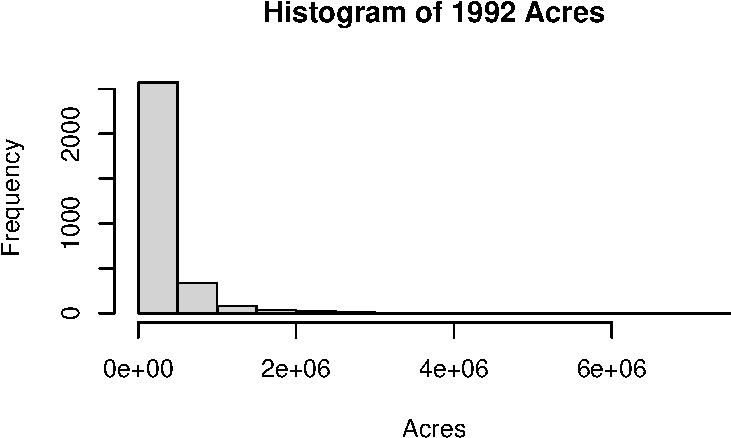
\includegraphics[keepaspectratio]{introR_files/figure-pdf/fig-agpop-acres92-hist-1.pdf}}

}

\caption{\label{fig-agpop-acres92-hist}Histogram of 1992 farm acreage}

\end{figure}%

\begin{Shaded}
\begin{Highlighting}[]
\FunctionTok{plot}\NormalTok{(agpop}\SpecialCharTok{$}\NormalTok{acres87, agpop}\SpecialCharTok{$}\NormalTok{acres92,}
     \AttributeTok{main =} \StringTok{"1992 vs 1987 Acreage"}\NormalTok{,}
     \AttributeTok{xlab =} \StringTok{"Acres 1987"}\NormalTok{, }\AttributeTok{ylab =} \StringTok{"Acres 1992"}\NormalTok{)}
\FunctionTok{abline}\NormalTok{(}\AttributeTok{a =} \DecValTok{0}\NormalTok{, }\AttributeTok{b =} \DecValTok{1}\NormalTok{, }\AttributeTok{col =} \StringTok{"red"}\NormalTok{)}
\end{Highlighting}
\end{Shaded}

\begin{figure}[H]

\centering{

\pandocbounded{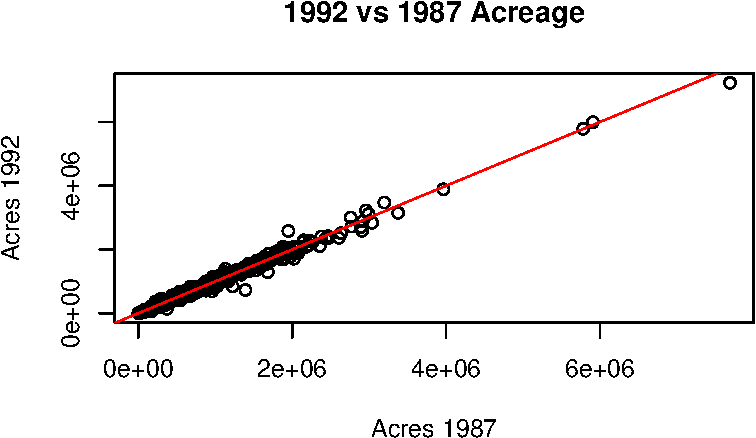
\includegraphics[keepaspectratio]{introR_files/figure-pdf/fig-agpop-acres-scatter-1.pdf}}

}

\caption{\label{fig-agpop-acres-scatter}1992 vs.~1987 farm acreage, with
the 1:1 line}

\end{figure}%

\subsection{Saving and re-inserting an external
plot}\label{saving-and-re-inserting-an-external-plot}

A high-resolution figure for a journal or a slide deck can be written
straight to disk: open a graphics device (\texttt{png()},
\texttt{pdf()}, \texttt{jpeg()}), run the plotting code, then close the
device with \texttt{dev.off()}. When \texttt{res} is raised,
\texttt{width} and \texttt{height} must be given in inches so the figure
does not shrink.

\begin{Shaded}
\begin{Highlighting}[]
\FunctionTok{dir.create}\NormalTok{(}\StringTok{"figures"}\NormalTok{, }\AttributeTok{showWarnings =} \ConstantTok{FALSE}\NormalTok{)}

\FunctionTok{png}\NormalTok{(}\StringTok{"figures/agpop\_scatter\_highres.png"}\NormalTok{,}
    \AttributeTok{width =} \DecValTok{6}\NormalTok{, }\AttributeTok{height =} \DecValTok{4}\NormalTok{, }\AttributeTok{units =} \StringTok{"in"}\NormalTok{, }\AttributeTok{res =} \DecValTok{300}\NormalTok{)}

\FunctionTok{plot}\NormalTok{(agpop}\SpecialCharTok{$}\NormalTok{acres87, agpop}\SpecialCharTok{$}\NormalTok{acres92,}
     \AttributeTok{main =} \StringTok{"1992 vs 1987 Acreage"}\NormalTok{,}
     \AttributeTok{xlab =} \StringTok{"Acres 1987"}\NormalTok{, }\AttributeTok{ylab =} \StringTok{"Acres 1992"}\NormalTok{)}
\FunctionTok{abline}\NormalTok{(}\AttributeTok{a =} \DecValTok{0}\NormalTok{, }\AttributeTok{b =} \DecValTok{1}\NormalTok{, }\AttributeTok{col =} \StringTok{"red"}\NormalTok{)}

\FunctionTok{dev.off}\NormalTok{()}
\end{Highlighting}
\end{Shaded}

The saved file can then be placed back into the document with
\texttt{knitr::include\_graphics()}.

\begin{Shaded}
\begin{Highlighting}[]
\NormalTok{knitr}\SpecialCharTok{::}\FunctionTok{include\_graphics}\NormalTok{(}\StringTok{"figures/agpop\_scatter\_highres.png"}\NormalTok{)}
\end{Highlighting}
\end{Shaded}

\begin{figure}[H]

\centering{

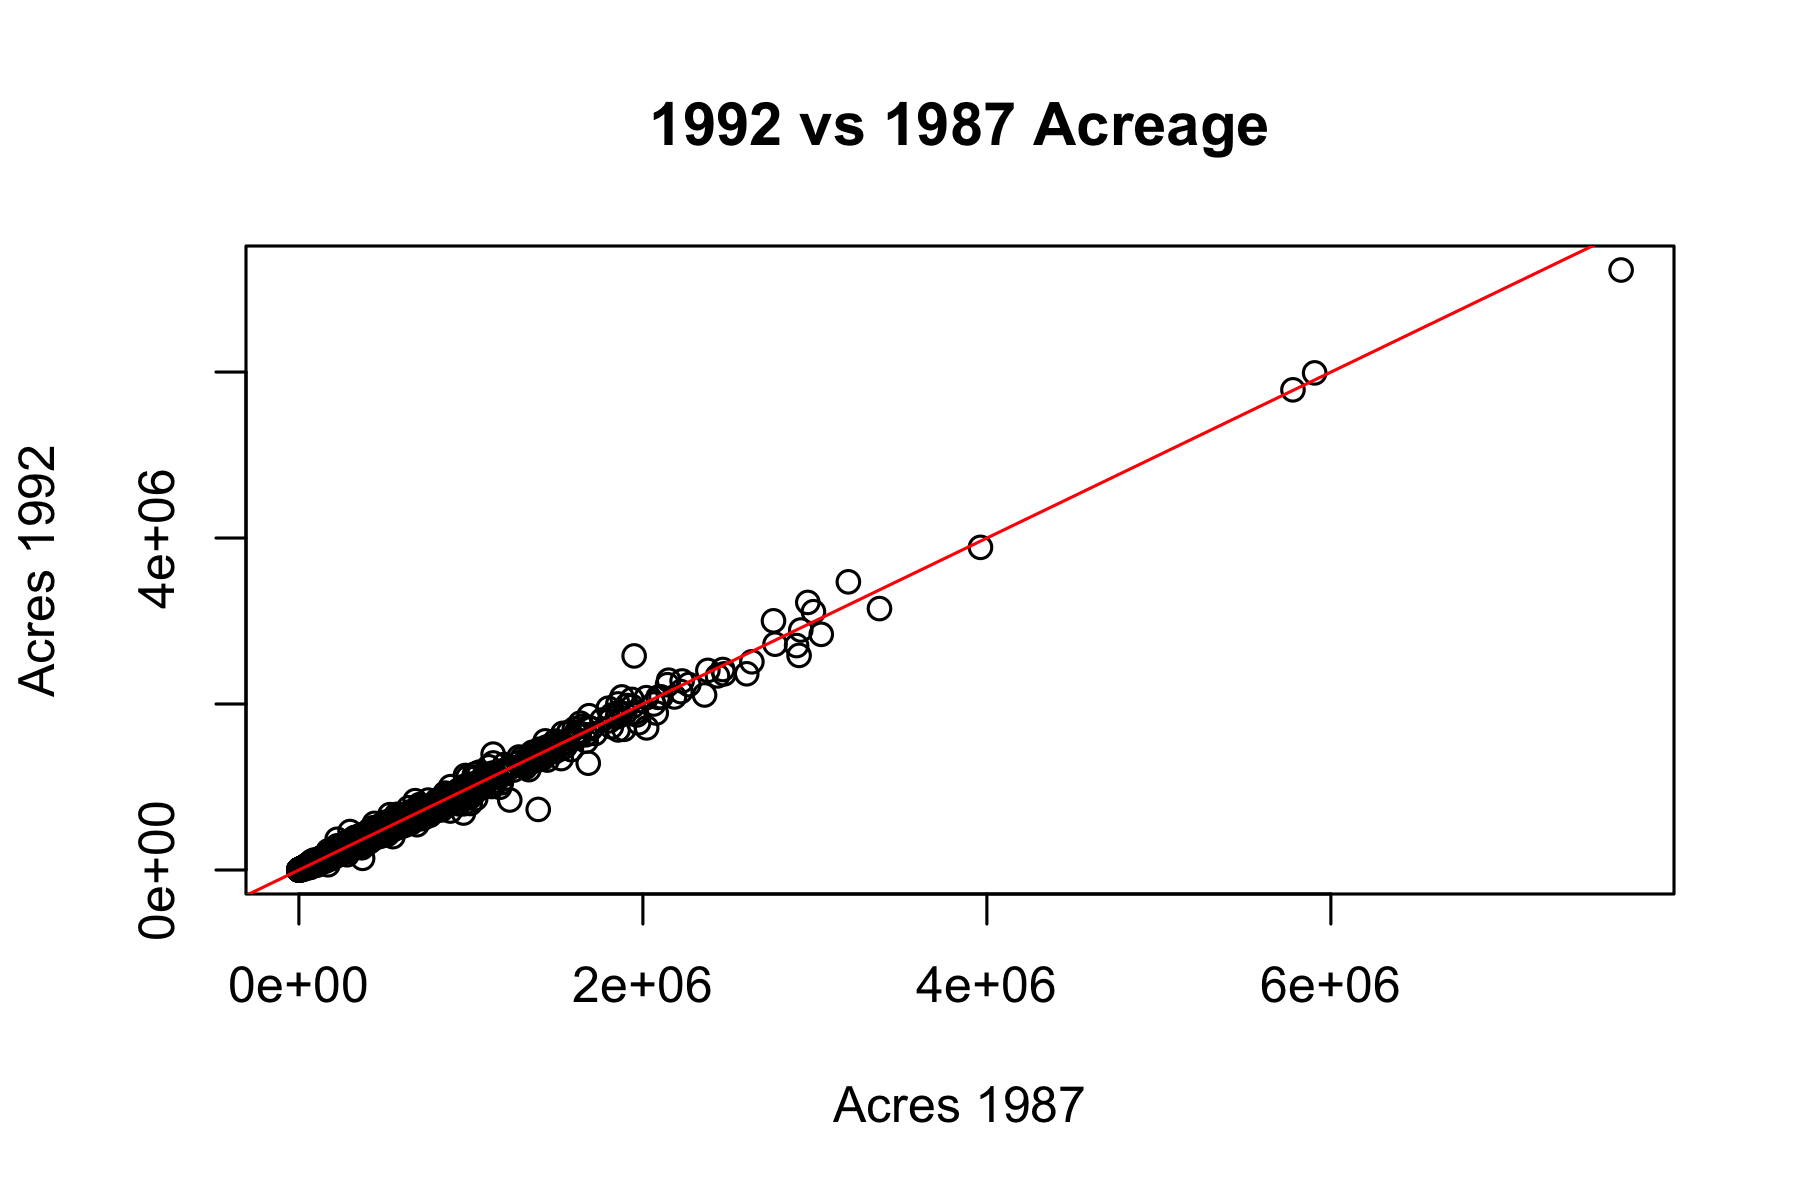
\includegraphics[width=6in,height=\textheight,keepaspectratio]{figures/agpop_scatter_highres.png}

}

\caption{\label{fig-agpop-scatter-highres}The saved high-resolution PNG,
re-inserted}

\end{figure}%

\subsection{Advanced visualization with
ggplot2}\label{advanced-visualization-with-ggplot2}

\texttt{ggplot2} provides a grammar of graphics for layered displays.
Below, a histogram of log-transformed 1992 acreage carries both an
empirical density curve and a fitted normal curve.

\begin{Shaded}
\begin{Highlighting}[]
\NormalTok{ag\_clean }\OtherTok{\textless{}{-}}\NormalTok{ agpop }\SpecialCharTok{|\textgreater{}}
  \FunctionTok{filter}\NormalTok{(}\SpecialCharTok{!}\FunctionTok{is.na}\NormalTok{(acres92), acres92 }\SpecialCharTok{\textgreater{}} \DecValTok{0}\NormalTok{) }\SpecialCharTok{|\textgreater{}}
  \FunctionTok{mutate}\NormalTok{(}\AttributeTok{log\_acres =} \FunctionTok{log}\NormalTok{(acres92))}

\NormalTok{mean\_log }\OtherTok{\textless{}{-}} \FunctionTok{mean}\NormalTok{(ag\_clean}\SpecialCharTok{$}\NormalTok{log\_acres)}
\NormalTok{sd\_log   }\OtherTok{\textless{}{-}} \FunctionTok{sd}\NormalTok{(ag\_clean}\SpecialCharTok{$}\NormalTok{log\_acres)}

\FunctionTok{ggplot}\NormalTok{(ag\_clean, }\FunctionTok{aes}\NormalTok{(}\AttributeTok{x =}\NormalTok{ log\_acres)) }\SpecialCharTok{+}
  \FunctionTok{geom\_histogram}\NormalTok{(}\FunctionTok{aes}\NormalTok{(}\AttributeTok{y =} \FunctionTok{after\_stat}\NormalTok{(density)), }\AttributeTok{bins =} \DecValTok{30}\NormalTok{,}
                 \AttributeTok{fill =} \StringTok{"steelblue"}\NormalTok{, }\AttributeTok{color =} \StringTok{"white"}\NormalTok{, }\AttributeTok{alpha =} \FloatTok{0.7}\NormalTok{) }\SpecialCharTok{+}
  \FunctionTok{geom\_density}\NormalTok{(}\AttributeTok{color =} \StringTok{"darkred"}\NormalTok{, }\AttributeTok{linewidth =} \FloatTok{1.2}\NormalTok{) }\SpecialCharTok{+}
  \FunctionTok{stat\_function}\NormalTok{(}
    \AttributeTok{fun =}\NormalTok{ dnorm,}
    \AttributeTok{args =} \FunctionTok{list}\NormalTok{(}\AttributeTok{mean =}\NormalTok{ mean\_log, }\AttributeTok{sd =}\NormalTok{ sd\_log),}
    \AttributeTok{color =} \StringTok{"black"}\NormalTok{, }\AttributeTok{linetype =} \StringTok{"dashed"}\NormalTok{, }\AttributeTok{linewidth =} \DecValTok{1}
\NormalTok{  ) }\SpecialCharTok{+}
  \FunctionTok{labs}\NormalTok{(}
    \AttributeTok{title =} \StringTok{"Distribution of Log(Acres92)"}\NormalTok{,}
    \AttributeTok{subtitle =} \StringTok{"Histogram with empirical density (red) and normal fit (black dashed)"}\NormalTok{,}
    \AttributeTok{x =} \StringTok{"Log of 1992 farm acreage"}\NormalTok{,}
    \AttributeTok{y =} \StringTok{"Density"}
\NormalTok{  ) }\SpecialCharTok{+}
  \FunctionTok{theme\_minimal}\NormalTok{()}
\end{Highlighting}
\end{Shaded}

\begin{figure}[H]

\centering{

\pandocbounded{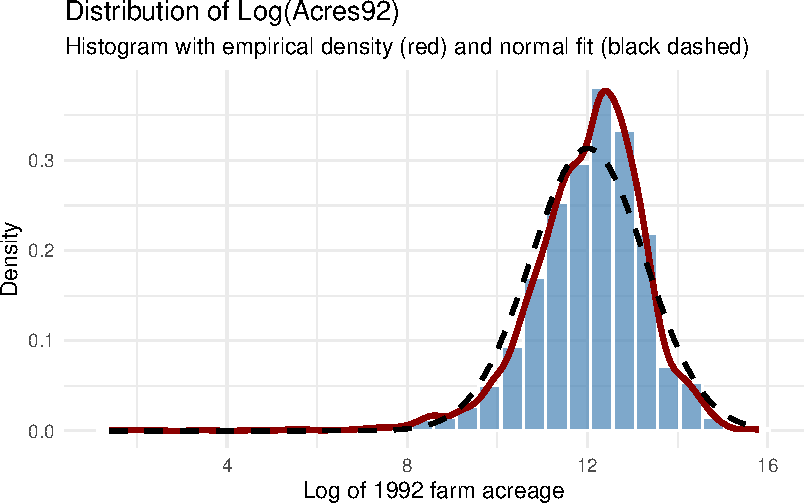
\includegraphics[keepaspectratio]{introR_files/figure-pdf/fig-log-acres-hist-1.pdf}}

}

\caption{\label{fig-log-acres-hist}Distribution of log(acres92):
histogram with empirical density and normal fit}

\end{figure}%

Mapping the histogram to \texttt{after\_stat(density)} puts it on the
same vertical scale as the two curves, so the three layers are directly
comparable.

\section{Writing your own function}\label{writing-your-own-function}

\begin{Shaded}
\begin{Highlighting}[]
\DocumentationTok{\#\# data is a matrix or data frame; returns the mean of each column}
\NormalTok{means\_col }\OtherTok{\textless{}{-}} \ControlFlowTok{function}\NormalTok{(data) \{}
\NormalTok{  n }\OtherTok{\textless{}{-}} \FunctionTok{ncol}\NormalTok{(data)}
\NormalTok{  cmeans }\OtherTok{\textless{}{-}} \FunctionTok{rep}\NormalTok{(}\ConstantTok{NA\_real\_}\NormalTok{, n)}
  \ControlFlowTok{for}\NormalTok{ (j }\ControlFlowTok{in} \FunctionTok{seq\_len}\NormalTok{(n)) \{}
\NormalTok{    cmeans[j] }\OtherTok{\textless{}{-}} \FunctionTok{mean}\NormalTok{(data[[j]], }\AttributeTok{na.rm =} \ConstantTok{TRUE}\NormalTok{)}
\NormalTok{  \}}
  \FunctionTok{names}\NormalTok{(cmeans) }\OtherTok{\textless{}{-}} \FunctionTok{colnames}\NormalTok{(data)}
\NormalTok{  cmeans}
\NormalTok{\}}
\end{Highlighting}
\end{Shaded}

Indexing with \texttt{data{[}{[}j{]}{]}} extracts column \texttt{j} as a
vector for both data frames and tibbles, whereas \texttt{data{[},\ j{]}}
returns a one-column tibble in the tibble case. \texttt{seq\_len(n)} is
used in place of \texttt{1:n} so that a zero-column input yields an
empty loop rather than iterating over \texttt{1,\ 0}.

\begin{Shaded}
\begin{Highlighting}[]
\NormalTok{agpop\_numeric }\OtherTok{\textless{}{-}}\NormalTok{ agpop }\SpecialCharTok{|\textgreater{}} \FunctionTok{select}\NormalTok{(}\FunctionTok{where}\NormalTok{(is.numeric))}

\NormalTok{custom\_means  }\OtherTok{\textless{}{-}} \FunctionTok{means\_col}\NormalTok{(agpop\_numeric)}
\NormalTok{builtin\_means }\OtherTok{\textless{}{-}} \FunctionTok{colMeans}\NormalTok{(agpop\_numeric, }\AttributeTok{na.rm =} \ConstantTok{TRUE}\NormalTok{)}

\FunctionTok{data.frame}\NormalTok{(}
  \AttributeTok{Variable        =} \FunctionTok{colnames}\NormalTok{(agpop\_numeric),}
  \AttributeTok{Custom\_Function =}\NormalTok{ custom\_means,}
  \AttributeTok{Built\_in        =}\NormalTok{ builtin\_means,}
  \AttributeTok{row.names       =} \ConstantTok{NULL}
\NormalTok{) }\SpecialCharTok{|\textgreater{}}
  \FunctionTok{gt}\NormalTok{() }\SpecialCharTok{|\textgreater{}}
  \FunctionTok{tab\_header}\NormalTok{(}
    \AttributeTok{title =} \StringTok{"Comparing Mean Calculations"}\NormalTok{,}
    \AttributeTok{subtitle =} \StringTok{"Custom function vs. base R colMeans()"}
\NormalTok{  ) }\SpecialCharTok{|\textgreater{}}
  \FunctionTok{cols\_label}\NormalTok{(}
    \AttributeTok{Variable        =} \FunctionTok{md}\NormalTok{(}\StringTok{"**Variable**"}\NormalTok{),}
    \AttributeTok{Custom\_Function =} \FunctionTok{md}\NormalTok{(}\StringTok{"**Custom \textasciigrave{}means\_col()\textasciigrave{}**"}\NormalTok{),}
    \AttributeTok{Built\_in        =} \FunctionTok{md}\NormalTok{(}\StringTok{"**Base \textasciigrave{}colMeans()\textasciigrave{}**"}\NormalTok{)}
\NormalTok{  ) }\SpecialCharTok{|\textgreater{}}
  \FunctionTok{fmt\_number}\NormalTok{(}\AttributeTok{columns =} \FunctionTok{c}\NormalTok{(Custom\_Function, Built\_in), }\AttributeTok{decimals =} \DecValTok{2}\NormalTok{)}
\end{Highlighting}
\end{Shaded}

\begin{table}

\caption{\label{tbl-means-custom-vs-builtin}Comparing column means:
custom function vs.~base R colMeans()}

\centering{

\caption*{
{\large  Comparing Mean Calculations\normalsize } \\ 
{\normalsize  Custom function vs. base R colMeans()\normalsize }
} 
\normalsize
\begin{gtfit}{\linewidth}{lrr}
\toprule
\textbf{Variable} & \textbf{Custom \texttt{means\_col()}} & \textbf{Base \texttt{colMeans()}} \\ 
\midrule\addlinespace[2.5pt]
acres92 & 308,582.41 & 308,582.41 \\ 
acres87 & 315,373.71 & 315,373.71 \\ 
acres82 & 321,972.52 & 321,972.52 \\ 
farms92 & 625.50 & 625.50 \\ 
farms87 & 678.28 & 678.28 \\ 
farms82 & 728.06 & 728.06 \\ 
largef92 & 56.18 & 56.18 \\ 
largef87 & 54.86 & 54.86 \\ 
largef82 & 52.62 & 52.62 \\ 
smallf92 & 54.09 & 54.09 \\ 
smallf87 & 59.54 & 59.54 \\ 
smallf82 & 60.97 & 60.97 \\ 
\bottomrule
\end{gtfit}

}

\end{table}%

\begin{Shaded}
\begin{Highlighting}[]
\FunctionTok{all.equal}\NormalTok{(custom\_means, builtin\_means)}
\end{Highlighting}
\end{Shaded}

\begin{verbatim}
[1] TRUE
\end{verbatim}

Selecting numeric columns with \texttt{where(is.numeric)} is preferable
to the positional \texttt{select(3:13)}, which breaks silently if the
column order of the source file changes. The \texttt{all.equal()} result
confirms agreement with the optimized built-in.

\bookmarksetup{startatroot}

\chapter{Simple Random Sampling}\label{simple-random-sampling}

Simple random sampling is the simplest probability sampling design, and
the building block for all the designs in later chapters. A stratified
sample is an SRS within each stratum; a cluster sample is an SRS of
clusters. This chapter defines the design, derives its estimators and
their standard errors, shows how to build confidence intervals and
choose the sample size, and checks the theory by simulation. The
material corresponds to Sections 2.3--2.6 and 2.8 of Lohr and Sections
4.1--4.5 of Scheaffer et al.

\section{SRS and SRSWR}\label{sec-srs-design}

There are two versions of simple random sampling.

A \textbf{simple random sample with replacement (SRSWR)} of size \(n\)
from a population of \(N\) units can be thought of as \(n\) independent
draws of one unit, each unit having probability \(1/N\) on every draw.
The same unit can be drawn more than once.

A \textbf{simple random sample without replacement (SRS)} of size \(n\)
is selected so that every possible subset of \(n\) distinct units in the
population has the same probability of being the sample. There are
\(\binom{N}{n}\) such subsets, so \[
P(\mathcal S) = \frac{1}{\binom{N}{n}} = \frac{n!\,(N-n)!}{N!}
\] for every subset \(\mathcal S\) of size \(n\). Unless stated
otherwise, ``SRS'' in this book means sampling without replacement. In
practice an SRS is drawn with computer-generated random numbers; in R,

\begin{Shaded}
\begin{Highlighting}[]
\FunctionTok{sample}\NormalTok{(}\DecValTok{1}\SpecialCharTok{:}\NormalTok{N, }\AttributeTok{size =}\NormalTok{ n)}
\end{Highlighting}
\end{Shaded}

returns the labels of \(n\) distinct units chosen in this way.

Figure~\ref{fig-srs-design} illustrates an SRS of \(n = 60\) from a
synthetic population of \(N = 1000\) units. The design uses no
information about the units other than their labels, so the sampled
units (red) are scattered at random over the population, and their
values cover its whole range.

\begin{figure}

\centering{

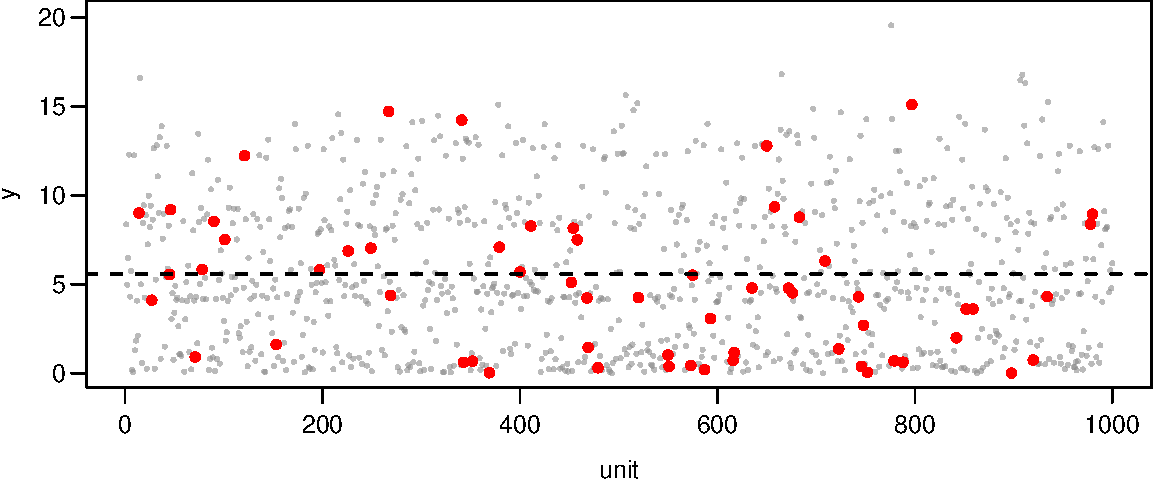
\includegraphics[width=0.85\linewidth,height=\textheight,keepaspectratio]{srs_files/figure-pdf/fig-srs-design-1.pdf}

}

\caption{\label{fig-srs-design}A simple random sample of \(n = 60\)
(red) from a synthetic population of \(N = 1000\) units, listed in an
arbitrary order. The dashed line is the population mean.}

\end{figure}%

\subsection{Inclusion probabilities}\label{inclusion-probabilities}

To study which units end up in the sample, define the sample-membership
indicator \[
Z_i = \begin{cases} 1 & \text{if unit } i \text{ is in the sample,} \\ 0 & \text{otherwise.} \end{cases}
\] The probability \(\pi_i = P(Z_i = 1)\) is the \textbf{inclusion
probability} of unit \(i\). If unit \(i\) is in the sample, the other
\(n-1\) sampled units must come from the remaining \(N-1\) units, so \[
\pi_i = P(Z_i=1) = \frac{\text{number of samples including unit } i}{\text{number of possible samples}}
 = \frac{\binom{N-1}{n-1}}{\binom{N}{n}} = \frac{n}{N}.
\] Every unit has the same chance \(n/N\) of being in the sample. The
indicators \(Z_1, \ldots, Z_N\) are the only random quantities in
design-based inference; we use them in
Section~\ref{sec-srs-randomization} to prove the properties of the
estimators.

\section{Estimators for Simple Random Sampling}\label{sec-srs-formulas}

Write \(y_i\) for the value of unit \(i\) in the population
\(U = \{1, \ldots, N\}\), and \[
\bar{y}_U = \frac{1}{N}\sum_{i=1}^N y_i, \qquad
t = \sum_{i=1}^N y_i = N\bar{y}_U, \qquad
S^2 = \frac{1}{N-1}\sum_{i=1}^N (y_i - \bar{y}_U)^2
\] for the population mean, total and variance. These are fixed, unknown
numbers.

\subsection{Estimating the population
mean}\label{estimating-the-population-mean}

The natural estimator of \(\bar y_U\) is the sample mean, and the
natural estimator of \(S^2\) is the sample variance: \[
\bar y = \frac1n \sum_{i \in \mathcal S} y_i = \frac1n \sum_{i=1}^N Z_i y_i,
\qquad
s^2 = \frac{1}{n-1}\sum_{i\in\mathcal S} (y_i - \bar y)^2 .
\] The sample mean is unbiased for \(\bar y_U\), and its variance is \[
V(\bar{y}) = \left(1 - \frac{n}{N}\right)\frac{S^2}{n}
\] (both are proved in Section~\ref{sec-srs-randomization}). This is the
familiar \(S^2/n\) of independent sampling, multiplied by the factor
\(1 - n/N\), the \textbf{finite population correction} (fpc). Sampling
without replacement removes units from the pool, so the sample covers
more of the population than independent draws would, and the variance is
smaller. When the sampling fraction \(n/N\) is small, the fpc is close
to \(1\) and can be ignored. When \(n = N\), the sample is a census and
\(V(\bar y) = 0\).

Since \(s^2\) is unbiased for \(S^2\) (also proved in
Section~\ref{sec-srs-randomization}), replacing \(S^2\) by \(s^2\) gives
an unbiased estimator of the variance. Its square root is the
\textbf{standard error}: \[
\boxed{
\hat{V}(\bar{y}) = \left(1 - \frac{n}{N}\right)\frac{s^2}{n}, \qquad
\mathrm{SE}(\bar y) = \sqrt{\Big(1-\frac nN\Big)\frac{s^2}{n}} .}
\]

\subsection{Estimating the population
total}\label{estimating-the-population-total}

Since \(t = N\bar y_U\), the total is estimated by scaling up the sample
mean: \[
\boxed{
\hat{t} = N\bar{y}, \qquad
\hat{V}(\hat{t}) = N^2\left(1 - \frac{n}{N}\right)\frac{s^2}{n}, \qquad
\mathrm{SE}(\hat{t}) = N\,\mathrm{SE}(\bar{y}).}
\]

\textbf{Sampling weights.} The estimated total can also be written with
\textbf{sampling weights}. The sampling weight of a unit is the
reciprocal of its inclusion probability, \(w_i = 1/\pi_i = N/n\), and \[
\hat t = \sum_{i\in\mathcal S} w_i y_i = \sum_{i\in\mathcal S} \frac{N}{n} y_i .
\] Each sampled unit ``represents'' \(N/n\) units of the population:
itself and \(N/n - 1\) unsampled ones. In an SRS all weights are equal;
in later chapters (stratified, cluster and unequal-probability sampling)
they are not, but the weighted-sum form of \(\hat t\) carries over.

\subsection{Coefficient of variation}\label{coefficient-of-variation}

The standard error is in the units of \(y\). A scale-free measure of
precision is the \textbf{coefficient of variation} (CV), defined when
\(\bar y_U \ne 0\): \[
\mathrm{CV}(\bar y) = \frac{\sqrt{V(\bar y)}}{E(\bar y)}
 = \sqrt{1-\frac nN}\ \frac{S}{\sqrt n\, \bar y_{U}},
\qquad
\widehat{\mathrm{CV}}(\bar y) = \frac{\mathrm{SE}(\bar y)}{\bar y} .
\] Because \(\hat t = N\bar y\), the factor \(N\) cancels and
\(\mathrm{CV}(\hat t) = \mathrm{CV}(\bar y)\). A CV of 0.05 means the
standard error is 5\% of the estimate, whatever the units of
measurement.

\subsection{Estimating a proportion}\label{estimating-a-proportion}

Estimating a proportion is a special case of estimating a mean. Define
\(y_i=1\) if unit \(i\) has the characteristic of interest and \(y_i=0\)
otherwise. Then the population proportion and the sample proportion are
\[
p = \frac{1}{N}\sum_{i=1}^N y_i = \bar y_{U}, \qquad
\hat p = \frac1n\sum_{i\in\mathcal S} y_i = \bar y ,
\] so \(\hat p\) is unbiased for \(p\). For a 0/1 variable
\(y_i^2 = y_i\), and the variances simplify: \[
S^2 = \frac{N}{N-1}\,p(1-p), \qquad
s^2 = \frac{n}{n-1}\,\hat p(1-\hat p).
\] Substituting into the general formulas, \[
V(\hat p) = \Big(\frac{N-n}{N-1}\Big)\frac{p(1-p)}{n},
\qquad
\boxed{\hat V(\hat p) = \Big(1-\frac nN\Big)\frac{\hat p (1-\hat p)}{n-1}.}
\] The number of units with the characteristic, \(Np\), is estimated by
\(N\hat p\) with standard error \(N\,\mathrm{SE}(\hat p)\).

\section{Example: The Census of Agriculture}\label{sec-srs-agsrs}

The U.S. government conducts a Census of Agriculture every five years.
It collects data on all farms (any place producing \$1000 or more of
agricultural products) in the 50 states, for each of the \(N=3078\)
counties and county-equivalents. The file \texttt{agpop.csv} contains
the 1982, 1987 and 1992 farm data for the whole population. An SRS of
\(n=300\) counties was selected with computer-generated random numbers
and saved as \texttt{agsrs.csv}. We use it to estimate the mean and
total of \texttt{acres92}, the number of acres devoted to farms in 1992,
and the proportion of counties with fewer than 200,000 acres in farms.

Throughout the agriculture examples in this book, county acreages are
expressed in \textbf{thousands of acres}. The raw figures run into the
millions, and every mean, variance and total reads far more easily on
that scale. The helper \texttt{acres\_in\_thousands()} performs the
conversion as the data are read.

\subsection{Step-by-step calculation}\label{step-by-step-calculation}

We first compute the estimates directly from the formulas of
Section~\ref{sec-srs-formulas}.

\begin{Shaded}
\begin{Highlighting}[]
\DocumentationTok{\#\# read survey data}
\NormalTok{agsrs }\OtherTok{\textless{}{-}} \FunctionTok{read.csv}\NormalTok{ (}\StringTok{"data/agsrs.csv"}\NormalTok{)}
\DocumentationTok{\#\# work in thousands of acres, the unit used for every agriculture example here}
\NormalTok{agsrs[}\FunctionTok{c}\NormalTok{(}\StringTok{"acres92"}\NormalTok{, }\StringTok{"acres87"}\NormalTok{, }\StringTok{"acres82"}\NormalTok{)] }\OtherTok{\textless{}{-}}\NormalTok{ agsrs[}\FunctionTok{c}\NormalTok{(}\StringTok{"acres92"}\NormalTok{, }\StringTok{"acres87"}\NormalTok{, }\StringTok{"acres82"}\NormalTok{)] }\SpecialCharTok{/} \DecValTok{1000}
\FunctionTok{head}\NormalTok{(agsrs)}
\end{Highlighting}
\end{Shaded}

\begin{verbatim}
             county state acres92 acres87 acres82 farms92 farms87 farms82 largef92 largef87 largef82 smallf92
1     COFFEE COUNTY    AL 175.209 179.311 194.509     760     842     944       29       28       21       57
2    COLBERT COUNTY    AL 138.135 145.104 161.360     488     563     686       37       41       42       12
3      LAMAR COUNTY    AL  56.102  59.861  72.334     299     362     447        4        4        3       16
4    MARENGO COUNTY    AL 199.117 220.526 231.207     434     471     622       48       66       62       14
5     MARION COUNTY    AL  89.228 105.586 113.618     566     658     748        7        9        9       11
6 TUSCALOOSA COUNTY    AL  96.194 120.542 134.616     436     521     650       20       17       23       18
  smallf87 smallf82 region
1       47       66      S
2       44       47      S
3       20       30      S
4       11       28      S
5       23       27      S
6       32       29      S
\end{verbatim}

\begin{Shaded}
\begin{Highlighting}[]
\DocumentationTok{\#\# extract the variable of interest}
\NormalTok{sdata }\OtherTok{\textless{}{-}}\NormalTok{ agsrs}\SpecialCharTok{$}\NormalTok{acres92}
\NormalTok{N }\OtherTok{\textless{}{-}} \DecValTok{3078}

\DocumentationTok{\#\# do calculation}
\NormalTok{n }\OtherTok{\textless{}{-}} \FunctionTok{length}\NormalTok{ (sdata)}
\NormalTok{ybar }\OtherTok{\textless{}{-}} \FunctionTok{mean}\NormalTok{ (sdata)}
\NormalTok{s }\OtherTok{\textless{}{-}} \FunctionTok{sd}\NormalTok{ (sdata)}
\NormalTok{se.ybar }\OtherTok{\textless{}{-}} \FunctionTok{sqrt}\NormalTok{((}\DecValTok{1} \SpecialCharTok{{-}}\NormalTok{ n }\SpecialCharTok{/}\NormalTok{ N)) }\SpecialCharTok{*}\NormalTok{ s }\SpecialCharTok{/} \FunctionTok{sqrt}\NormalTok{(n)}
\NormalTok{mem }\OtherTok{\textless{}{-}} \FunctionTok{qt}\NormalTok{ (}\FloatTok{0.975}\NormalTok{, }\AttributeTok{df =}\NormalTok{ n }\SpecialCharTok{{-}} \DecValTok{1}\NormalTok{) }\SpecialCharTok{*}\NormalTok{ se.ybar}

\DocumentationTok{\#\# return estimate vector for pop mean}
\FunctionTok{c}\NormalTok{ (}\AttributeTok{Est. =}\NormalTok{ ybar, }\AttributeTok{S.E. =}\NormalTok{ se.ybar, }\AttributeTok{ci.low =}\NormalTok{ ybar }\SpecialCharTok{{-}}\NormalTok{ mem, }\AttributeTok{ci.upp =}\NormalTok{ ybar }\SpecialCharTok{+}\NormalTok{ mem)}
\end{Highlighting}
\end{Shaded}

\begin{verbatim}
     Est.      S.E.    ci.low    ci.upp 
297.89705  18.89843 260.70626 335.08784 
\end{verbatim}

\begin{Shaded}
\begin{Highlighting}[]
\DocumentationTok{\#\# return estimate vector for pop total}
\FunctionTok{c}\NormalTok{ (}\AttributeTok{Est. =}\NormalTok{ ybar, }\AttributeTok{S.E. =}\NormalTok{ se.ybar, }\AttributeTok{ci.low =}\NormalTok{ ybar }\SpecialCharTok{{-}}\NormalTok{ mem, }\AttributeTok{ci.upp =}\NormalTok{ ybar }\SpecialCharTok{+}\NormalTok{ mem) }\SpecialCharTok{*}\NormalTok{ N}
\end{Highlighting}
\end{Shaded}

\begin{verbatim}
      Est.       S.E.     ci.low     ci.upp 
 916927.11   58169.38  802453.86 1031400.36 
\end{verbatim}

In thousands of acres, the sample gives \(\bar y = 297.897\) and
\(s = 344.55\), so \[
\mathrm{SE}(\bar y) = \sqrt{\Big(1-\frac{300}{3078}\Big)\frac{344.55^2}{300}} = 18.898,
\] \[
\hat t = N\bar y = 3078(297.897) = 916,927,
\qquad
\mathrm{SE}(\hat t) = 3078(18.898) = 58,169 .
\] The average county has about 298 thousand acres in farms, and the
U.S. total is estimated at about 917 million acres. The estimated
coefficient of variation is \[
\widehat{\mathrm{CV}}(\hat t) = \widehat{\mathrm{CV}}(\bar y)
 = \frac{\mathrm{SE}(\bar y)}{\bar y}
 = \frac{18.898}{297.897} = 0.0634,
\] so the standard error is about 6.3\% of the estimate.

The data are highly skewed (Figure~\ref{fig-agsrs-acres92-hist}): most
counties have fewer than 500 thousand acres in farms, but some have more
than 1.5 million. For such data the mean is pulled up by the long right
tail, and we should also report the \textbf{median}, which is 196.7
thousand acres here, well below the mean.

\begin{Shaded}
\begin{Highlighting}[]
\FunctionTok{hist}\NormalTok{(sdata, }\AttributeTok{breaks =} \DecValTok{30}\NormalTok{, }\AttributeTok{col =} \StringTok{"lightblue"}\NormalTok{, }\AttributeTok{border =} \StringTok{"white"}\NormalTok{,}
     \AttributeTok{xlab =} \StringTok{"acres92 (thousands of acres)"}\NormalTok{, }\AttributeTok{main =} \StringTok{""}\NormalTok{)}
\FunctionTok{abline}\NormalTok{(}\AttributeTok{v =} \FunctionTok{c}\NormalTok{(ybar, }\FunctionTok{median}\NormalTok{(sdata)), }\AttributeTok{col =} \FunctionTok{c}\NormalTok{(}\StringTok{"firebrick"}\NormalTok{, }\StringTok{"darkgreen"}\NormalTok{), }\AttributeTok{lwd =} \DecValTok{2}\NormalTok{, }\AttributeTok{lty =} \FunctionTok{c}\NormalTok{(}\DecValTok{1}\NormalTok{, }\DecValTok{2}\NormalTok{))}
\FunctionTok{legend}\NormalTok{(}\StringTok{"topright"}\NormalTok{, }\AttributeTok{bty =} \StringTok{"n"}\NormalTok{, }\AttributeTok{lwd =} \DecValTok{2}\NormalTok{, }\AttributeTok{lty =} \FunctionTok{c}\NormalTok{(}\DecValTok{1}\NormalTok{, }\DecValTok{2}\NormalTok{), }\AttributeTok{col =} \FunctionTok{c}\NormalTok{(}\StringTok{"firebrick"}\NormalTok{, }\StringTok{"darkgreen"}\NormalTok{),}
       \AttributeTok{legend =} \FunctionTok{c}\NormalTok{(}\StringTok{"mean"}\NormalTok{, }\StringTok{"median"}\NormalTok{))}
\end{Highlighting}
\end{Shaded}

\begin{figure}[H]

\centering{

\pandocbounded{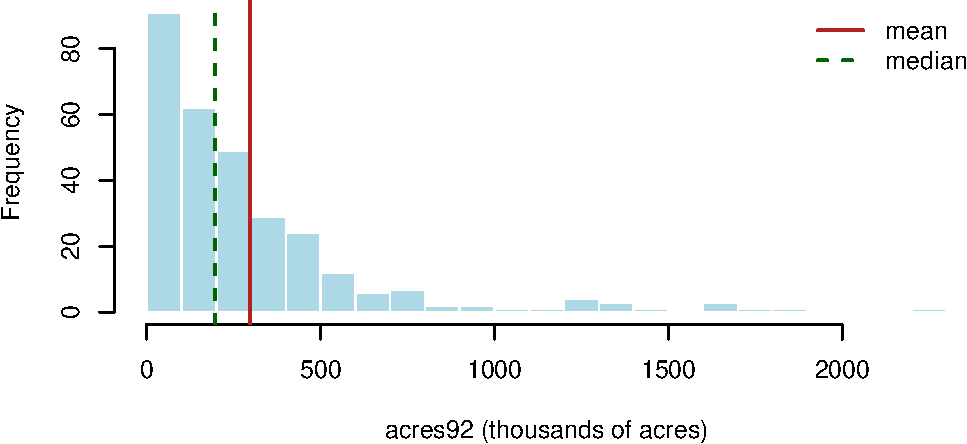
\includegraphics[keepaspectratio]{srs_files/figure-pdf/fig-agsrs-acres92-hist-1.pdf}}

}

\caption{\label{fig-agsrs-acres92-hist}Farm acreage in 1992 (thousands
of acres) for the SRS of 300 counties. The distribution is strongly
skewed to the right.}

\end{figure}%

\textbf{A proportion.} Let \(y_i = 1\) if county \(i\) has fewer than
200 thousand acres in farms. In the sample, 153 of the 300 counties do,
so \(\hat p = 153/300 = 0.51\) and \[
\mathrm{SE}(\hat p) = \sqrt{\Big(1-\frac{300}{3078}\Big)\frac{(0.51)(0.49)}{299}} = 0.0275 .
\]

\subsection{A function for repeated
use}\label{a-function-for-repeated-use}

The same calculation is needed again and again, so we wrap it in a
function. To avoid repeating code in every chapter, all estimating
functions (and their \texttt{gt} table formatting helpers) live in a
single shared file, \texttt{samplingestimate.r}, sourced at the start of
this chapter. The SRS function is \texttt{srs\_est()}.

The full source of \texttt{samplingestimate.r} is listed in
Appendix~\ref{sec-estimating-functions}.

\begin{Shaded}
\begin{Highlighting}[]
\NormalTok{agsrs }\OtherTok{\textless{}{-}} \FunctionTok{acres\_in\_thousands}\NormalTok{ (}\FunctionTok{read.csv}\NormalTok{ (}\StringTok{"data/agsrs.csv"}\NormalTok{))}
\end{Highlighting}
\end{Shaded}

\emph{Estimating the mean of acres92.} The function's \texttt{\$table}
shows the row-level working values (the first 6 rows and the Sum), and
\texttt{\$estimate} holds the point estimate, SE and CI, formatted with
\texttt{format\_est\_gt()}.

\begin{Shaded}
\begin{Highlighting}[]
\NormalTok{res\_mean }\OtherTok{\textless{}{-}} \FunctionTok{srs\_est}\NormalTok{(agsrs[,}\StringTok{"acres92"}\NormalTok{], }\AttributeTok{N =} \DecValTok{3078}\NormalTok{, }\AttributeTok{estimate =} \StringTok{"mean"}\NormalTok{)}
\NormalTok{res\_mean}\SpecialCharTok{$}\NormalTok{table}
\end{Highlighting}
\end{Shaded}

\begin{table}[H]
\caption*{
{\large  SRS Mean Estimation: Working Table\normalsize } \\ 
{\normalsize  \(n = 300\)\normalsize }
} 
\normalsize
\begin{gtfit}{\linewidth}{>{\raggedright\arraybackslash}p{\dimexpr 30.00pt -2\tabcolsep-1.5\arrayrulewidth}>{\raggedleft\arraybackslash}p{\dimexpr 82.50pt -2\tabcolsep-1.5\arrayrulewidth}>{\raggedleft\arraybackslash}p{\dimexpr 82.50pt -2\tabcolsep-1.5\arrayrulewidth}>{\raggedleft\arraybackslash}p{\dimexpr 82.50pt -2\tabcolsep-1.5\arrayrulewidth}>{\raggedleft\arraybackslash}p{\dimexpr 82.50pt -2\tabcolsep-1.5\arrayrulewidth}}
\toprule
\(i\) & \(y_i\) & \(\hat y_i\) & \(e_i\) & \((y_i-\hat y_i)^2\)\textsuperscript{\textit{1}} \\ 
\midrule\addlinespace[2.5pt]
1 & 175.21 & 297.90 & -122.69 & 15,052.36 \\ 
2 & 138.13 & 297.90 & -159.76 & 25,523.91 \\ 
3 & 56.10 & 297.90 & -241.80 & 58,464.84 \\ 
4 & 199.12 & 297.90 & -98.78 & 9,757.50 \\ 
5 & 89.23 & 297.90 & -208.67 & 43,542.77 \\ 
6 & 96.19 & 297.90 & -201.70 & 40,684.12 \\ 
... & ... & ... & ... & ... \\ 
{\bfseries Sum} & {\bfseries 89,369.11} & {\bfseries 297.90} & {\bfseries 0.00} & {\bfseries 35,496,086.45} \\ 
\bottomrule
\end{gtfit}
\begin{minipage}{\linewidth}
\vspace{.05em}
\textsuperscript{\textit{1}}\(\hat y_i = \bar y\) for every unit under the SRS model; \(s_y^2 = \sum_i (y_i-\hat y_i)^2/(n-1) = 1.19 \times 10^{5}\).\\
\(\bar y = \dfrac{\sum_i y_i}{n} = \dfrac{89,369.11}{300} = 297.90\)\\
\(\mathrm{SE}(\bar y) = \sqrt{1-\dfrac{n}{N}}\,\dfrac{s_y}{\sqrt n} = \sqrt{1-\dfrac{300}{3078}}\,\dfrac{344.55}{\sqrt{300}} = 18.90\)\\
\end{minipage}
\end{table}

\begin{Shaded}
\begin{Highlighting}[]
\NormalTok{res\_mean}\SpecialCharTok{$}\NormalTok{estimate }\SpecialCharTok{|\textgreater{}} \FunctionTok{format\_est\_gt}\NormalTok{(}\StringTok{"mean"}\NormalTok{)}
\end{Highlighting}
\end{Shaded}

\begin{table}[H]
\normalsize
\begin{gtfit}{0.7\linewidth}{rrrr}
\toprule
\(\bar{y}\) & \(\mathrm{SE}(\bar{y})\) & 95\% CI Lower & 95\% CI Upper \\ 
\midrule\addlinespace[2.5pt]
297.90 & 18.90 & 260.71 & 335.09 \\ 
\bottomrule
\end{gtfit}
\end{table}

\emph{Estimating the total of acres92.} Setting
\texttt{estimate\ =\ "total"} makes the function scale the mean and
confidence interval by \(N = 3078\).

\begin{Shaded}
\begin{Highlighting}[]
\NormalTok{res\_total }\OtherTok{\textless{}{-}} \FunctionTok{srs\_est}\NormalTok{(agsrs[,}\StringTok{"acres92"}\NormalTok{], }\AttributeTok{N =} \DecValTok{3078}\NormalTok{, }\AttributeTok{estimate =} \StringTok{"total"}\NormalTok{, }\AttributeTok{show.details =} \ConstantTok{FALSE}\NormalTok{)}
\NormalTok{res\_total}\SpecialCharTok{$}\NormalTok{estimate }\SpecialCharTok{|\textgreater{}} \FunctionTok{format\_est\_gt}\NormalTok{(}\StringTok{"total"}\NormalTok{)}
\end{Highlighting}
\end{Shaded}

\begin{table}[H]
\normalsize
\begin{gtfit}{0.7\linewidth}{rrrr}
\toprule
\(\hat{t}\) & \(\mathrm{SE}(\hat{t})\) & 95\% CI Lower & 95\% CI Upper \\ 
\midrule\addlinespace[2.5pt]
916,927.11 & 58,169.38 & 802,453.86 & 1,031,400.36 \\ 
\bottomrule
\end{gtfit}
\end{table}

\emph{Estimating the proportion of counties with fewer than 200K acres.}
We create the 0/1 indicator and estimate its mean.

\begin{Shaded}
\begin{Highlighting}[]
\NormalTok{acres92.is.fewer}\FloatTok{.200}\NormalTok{k }\OtherTok{\textless{}{-}} \FunctionTok{as.numeric}\NormalTok{ (agsrs[,}\StringTok{"acres92"}\NormalTok{] }\SpecialCharTok{\textless{}} \DecValTok{200}\NormalTok{)   }\CommentTok{\# 200 thousand acres}
\FunctionTok{head}\NormalTok{(acres92.is.fewer}\FloatTok{.200}\NormalTok{k)}
\end{Highlighting}
\end{Shaded}

\begin{verbatim}
[1] 1 1 1 1 1 1
\end{verbatim}

\begin{Shaded}
\begin{Highlighting}[]
\NormalTok{res\_prop }\OtherTok{\textless{}{-}} \FunctionTok{srs\_est}\NormalTok{(acres92.is.fewer}\FloatTok{.200}\NormalTok{k, }\AttributeTok{N =} \DecValTok{3078}\NormalTok{, }\AttributeTok{estimate =} \StringTok{"mean"}\NormalTok{, }\AttributeTok{show.details =} \ConstantTok{FALSE}\NormalTok{)}
\NormalTok{res\_prop}\SpecialCharTok{$}\NormalTok{estimate }\SpecialCharTok{|\textgreater{}} \FunctionTok{format\_est\_gt}\NormalTok{(}\StringTok{"mean"}\NormalTok{)}
\end{Highlighting}
\end{Shaded}

\begin{table}[H]
\normalsize
\begin{gtfit}{0.7\linewidth}{rrrr}
\toprule
\(\bar{y}\) & \(\mathrm{SE}(\bar{y})\) & 95\% CI Lower & 95\% CI Upper \\ 
\midrule\addlinespace[2.5pt]
0.51 & 0.03 & 0.46 & 0.56 \\ 
\bottomrule
\end{gtfit}
\end{table}

\emph{Estimating the number of such counties.}

\begin{Shaded}
\begin{Highlighting}[]
\NormalTok{res\_prop\_total }\OtherTok{\textless{}{-}} \FunctionTok{srs\_est}\NormalTok{(acres92.is.fewer}\FloatTok{.200}\NormalTok{k, }\AttributeTok{N =} \DecValTok{3078}\NormalTok{, }\AttributeTok{estimate =} \StringTok{"total"}\NormalTok{, }\AttributeTok{show.details =} \ConstantTok{FALSE}\NormalTok{)}
\NormalTok{res\_prop\_total}\SpecialCharTok{$}\NormalTok{estimate }\SpecialCharTok{|\textgreater{}} \FunctionTok{format\_est\_gt}\NormalTok{(}\StringTok{"total"}\NormalTok{)}
\end{Highlighting}
\end{Shaded}

\begin{table}[H]
\normalsize
\begin{gtfit}{0.7\linewidth}{rrrr}
\toprule
\(\hat{t}\) & \(\mathrm{SE}(\hat{t})\) & 95\% CI Lower & 95\% CI Upper \\ 
\midrule\addlinespace[2.5pt]
1,569.78 & 84.54 & 1,403.42 & 1,736.14 \\ 
\bottomrule
\end{gtfit}
\end{table}

\subsection{Comparing with the true
values}\label{comparing-with-the-true-values}

Because the census file \texttt{agpop.csv} contains the whole
population, we can check how close the SRS estimates came to the true
values. (In a real survey these are, of course, unknown.)

\begin{Shaded}
\begin{Highlighting}[]
\NormalTok{agpop }\OtherTok{\textless{}{-}} \FunctionTok{acres\_in\_thousands}\NormalTok{ (}\FunctionTok{read.csv}\NormalTok{ (}\StringTok{"data/agpop.csv"}\NormalTok{))}
\CommentTok{\#true mean (thousands of acres)}
\FunctionTok{mean}\NormalTok{ (agpop[, }\StringTok{"acres92"}\NormalTok{], }\AttributeTok{na.rm =}\NormalTok{ T)}
\end{Highlighting}
\end{Shaded}

\begin{verbatim}
[1] 308.5824
\end{verbatim}

\begin{Shaded}
\begin{Highlighting}[]
\CommentTok{\# true total (thousands of acres)}
\FunctionTok{sum}\NormalTok{ (agpop[, }\StringTok{"acres92"}\NormalTok{], }\AttributeTok{na.rm =}\NormalTok{ T)}
\end{Highlighting}
\end{Shaded}

\begin{verbatim}
[1] 943953.6
\end{verbatim}

\begin{Shaded}
\begin{Highlighting}[]
\CommentTok{\# true proportion of counties with less than 200K acres for farming}
\FunctionTok{mean}\NormalTok{ (agpop[, }\StringTok{"acres92"}\NormalTok{] }\SpecialCharTok{\textless{}} \DecValTok{200}\NormalTok{, }\AttributeTok{na.rm =}\NormalTok{ T)}
\end{Highlighting}
\end{Shaded}

\begin{verbatim}
[1] 0.5145472
\end{verbatim}

\begin{Shaded}
\begin{Highlighting}[]
\CommentTok{\# true number of counties with less than 200K acres for farming}
\FunctionTok{sum}\NormalTok{ (agpop[, }\StringTok{"acres92"}\NormalTok{] }\SpecialCharTok{\textless{}} \DecValTok{200}\NormalTok{, }\AttributeTok{na.rm =}\NormalTok{ T)}
\end{Highlighting}
\end{Shaded}

\begin{verbatim}
[1] 1574
\end{verbatim}

All the true values lie inside the 95\% confidence intervals computed
above.

\section{Confidence Intervals}\label{sec-srs-ci}

A confidence interval (CI) indicates the accuracy of an estimate. A 95\%
CI is often explained heuristically: if we took samples from the
population over and over again, and constructed a CI by our procedure
for each possible sample, we would expect 95\% of the resulting
intervals to include the true value of the population quantity. In
design-based inference this is literally what the probability refers to:
the population is fixed and the randomness is over the \(\binom{N}{n}\)
possible samples.

\subsection{Normality of the sample
mean}\label{normality-of-the-sample-mean}

In an SRS without replacement the observations are not independent, so
the ordinary central limit theorem does not apply directly. A
finite-population version is due to Hájek (1960): if certain technical
conditions hold and \(n\), \(N\) and \(N-n\) are all ``sufficiently
large'', then the sampling distribution of \[
\frac{\bar y - \bar y_{U}}{\sqrt{\big(1-\tfrac nN\big)}\, \tfrac{S}{\sqrt n}}
\] is approximately standard normal. Replacing \(S\) by \(s\) gives the
standard error, and approximate \(100(1-\alpha)\%\) CIs for the mean,
total and proportion are \[
\bar y \pm t_{\alpha/2,\, n-1} \, \mathrm{SE}(\bar y), \qquad
\hat t \pm t_{\alpha/2,\, n-1} \, \mathrm{SE}(\hat t), \qquad
\hat p \pm t_{\alpha/2,\, n-1} \, \mathrm{SE}(\hat p).
\] The \(t\) quantile is customary; for the sample sizes used in surveys
it is very close to the normal quantile \(z_{\alpha/2}\).

\textbf{Example (continued).} For the agriculture sample,
\(t_{0.025,\,299} = 1.968\), and the 95\% CIs are \[
\text{mean: } 297.9 \pm 1.968(18.9) = [260.7,\ 335.1] \text{ thousand acres},
\] \[
\text{total: } [802,454,\ 1,031,400] \text{ thousand acres},
\] \[
\text{proportion: } 0.51 \pm 1.968(0.0275) = [0.456,\ 0.564],
\] matching the output of \texttt{srs\_est()} in
Section~\ref{sec-srs-agsrs}.

\subsection{\texorpdfstring{How large must \(n\) be for
normality?}{How large must n be for normality?}}\label{how-large-must-n-be-for-normality}

The normal approximation needs a larger sample when the population is
skewed, as acreage is. Sugden, Smith and Jones (2000) extend Cochran's
rule and recommend the minimum sample size \[
n_{\min} = 28 + 25\left(\frac{\sum_{i=1}^N (y_i-\bar y_{U})^3}{N S^3}\right)^{\!2},
\] where the quantity in parentheses is the \textbf{skewness} of the
population. The more skewed the population, the larger the sample
required.

\begin{Shaded}
\begin{Highlighting}[]
\NormalTok{g1 }\OtherTok{\textless{}{-}}\NormalTok{ (}\FunctionTok{sum}\NormalTok{((sdata }\SpecialCharTok{{-}}\NormalTok{ ybar)}\SpecialCharTok{\^{}}\DecValTok{3}\NormalTok{) }\SpecialCharTok{/}\NormalTok{ n) }\SpecialCharTok{/}\NormalTok{ s}\SpecialCharTok{\^{}}\DecValTok{3}   \CommentTok{\# sample skewness}
\NormalTok{n\_min }\OtherTok{\textless{}{-}} \DecValTok{28} \SpecialCharTok{+} \DecValTok{25} \SpecialCharTok{*}\NormalTok{ g1}\SpecialCharTok{\^{}}\DecValTok{2}
\FunctionTok{c}\NormalTok{(}\AttributeTok{skewness =}\NormalTok{ g1, }\AttributeTok{n\_min =}\NormalTok{ n\_min)}
\end{Highlighting}
\end{Shaded}

\begin{verbatim}
  skewness      n_min 
  2.567866 192.848373 
\end{verbatim}

For the agriculture data we substitute the sample quantities:
\(s = 344.55\) and
\(\sum_{i\in\mathcal S}(y_i-\bar y)^3/n = 1.0504 \times 10^{8}\) (in
thousands of acres), giving a skewness of 2.57 and \[
n_{\min} = 28 + 25(2.568)^2 \approx 193 .
\] Our sample of \(n=300\) exceeds \(n_{\min}\), so it appears large
enough for the sampling distribution of \(\bar y\) to be approximately
normal. The simulation in Section~\ref{sec-srs-simulation} confirms
this.

\section{Choosing the Sample Size}\label{sec-srs-sample-size}

Before a survey is carried out we must decide how large the sample
should be. The answer depends on how precise the estimate must be.

\subsection{Specifying the tolerable
error}\label{specifying-the-tolerable-error}

The desired precision is often expressed in absolute terms, \[
P(|\bar y - \bar y_{U}| \le e) = 1-\alpha ,
\] where \(e\) is the \textbf{margin of error}. For many surveys of
people that measure a proportion, \(e=0.03\) and \(\alpha=0.05\).
Alternatively, precision can be specified in relative terms, which
controls the CV: \[
P\left(\left|\frac{\bar y - \bar y_{U}}{\bar y_{U}}\right| \le r\right) = 1-\alpha,
\qquad\text{that is,}\qquad e = r \, \bar y_{U} .
\] For example, if \(\bar y_{U} \approx 180\) thousand and \(r=0.1\),
then \(e=18\) thousand.

\subsection{\texorpdfstring{Solving for
\(n\)}{Solving for n}}\label{solving-for-n}

Using the normal approximation, the margin of error is
\(z_{\alpha/2}\,\mathrm{SD}(\bar y)\), so we need \(n\) with \[
e = z_{\alpha/2}\sqrt{\Big(1-\frac nN\Big)\frac{S^2}{n}} .
\] Solving in two steps is convenient. First find the sample size
\(n_0\) we would need for an infinite population (no fpc): \[
n_0 = \left(\frac{z_{\alpha/2}\, S}{e}\right)^{\!2}.
\] Then adjust for the finite population: \[
\boxed{n = \frac{n_0}{1+n_0/N} = \frac{z_{\alpha/2}^2 S^2}{e^2 + z_{\alpha/2}^2 S^2/N}.}
\] When \(N\) is large relative to \(n_0\), \(n \approx n_0\); the
population size matters only when \(n_0\) is a substantial fraction of
\(N\). The formula needs a value for \(S\), which is unknown. It can
come from a pilot sample, a previous survey of a similar population, or
a guess. For a proportion, \(S^2 \approx p(1-p) \le 1/4\), so using
\(p = 1/2\) gives a conservative (largest) sample size.

\begin{Shaded}
\begin{Highlighting}[]
\NormalTok{srs\_size }\OtherTok{\textless{}{-}} \ControlFlowTok{function}\NormalTok{(S, e, }\AttributeTok{N =} \ConstantTok{Inf}\NormalTok{, }\AttributeTok{alpha =} \FloatTok{0.05}\NormalTok{) \{}
\NormalTok{  n0 }\OtherTok{\textless{}{-}}\NormalTok{ (}\FunctionTok{qnorm}\NormalTok{(}\DecValTok{1} \SpecialCharTok{{-}}\NormalTok{ alpha }\SpecialCharTok{/} \DecValTok{2}\NormalTok{) }\SpecialCharTok{*}\NormalTok{ S }\SpecialCharTok{/}\NormalTok{ e)}\SpecialCharTok{\^{}}\DecValTok{2}
  \FunctionTok{c}\NormalTok{(}\AttributeTok{n0 =}\NormalTok{ n0, }\AttributeTok{n =}\NormalTok{ n0 }\SpecialCharTok{/}\NormalTok{ (}\DecValTok{1} \SpecialCharTok{+}\NormalTok{ n0 }\SpecialCharTok{/}\NormalTok{ N))}
\NormalTok{\}}
\end{Highlighting}
\end{Shaded}

\textbf{Example: margin of error 0.03 for a proportion.} We want to
estimate the proportion of the \(N=1251\) recipes in a cookbook that do
not involve animal products, with a 95\% CI of margin of error 0.03.
Using the conservative \(p = 1/2\), \[
n_0 = \frac{(1.96)^2 (\tfrac12)(1-\tfrac12)}{(0.03)^2} \approx 1067 .
\] Since \(n_0\) is large relative to \(N=1251\), the fpc adjustment
matters: \[
n = \frac{n_0}{1+n_0/N} = \frac{1067}{1+1067/1251} \approx 576 .
\] If \(N\) were very large we would use \(n\approx n_0 = 1067\).

\begin{Shaded}
\begin{Highlighting}[]
\FunctionTok{srs\_size}\NormalTok{(}\AttributeTok{S =} \FloatTok{0.5}\NormalTok{, }\AttributeTok{e =} \FloatTok{0.03}\NormalTok{, }\AttributeTok{N =} \DecValTok{1251}\NormalTok{)}
\end{Highlighting}
\end{Shaded}

\begin{verbatim}
       n0         n 
1067.0719  575.8695 
\end{verbatim}

\textbf{Example: the agriculture survey.} A pilot sample of 30 counties
was taken (one county was missing \texttt{acres92}). The sample SD of
the remaining 29 observations was 519.085 thousand acres. With a desired
margin of error of 60 thousand acres, \[
n_0 = (1.96)^2\,\frac{519.085^2}{60^2} \approx 288,
\qquad
n = \frac{288}{1+288/3078} \approx 263 .
\] The investigators took a sample of 300, in case the pilot's estimate
of the SD was too low.

\begin{Shaded}
\begin{Highlighting}[]
\FunctionTok{srs\_size}\NormalTok{(}\AttributeTok{S =} \FloatTok{519.085}\NormalTok{, }\AttributeTok{e =} \DecValTok{60}\NormalTok{, }\AttributeTok{N =} \DecValTok{3078}\NormalTok{)}
\end{Highlighting}
\end{Shaded}

\begin{verbatim}
      n0        n 
287.5217 262.9583 
\end{verbatim}

\section{Randomization Theory for SRS}\label{sec-srs-randomization}

We now prove the properties of \(\bar y\) and \(s^2\) used above. In the
\textbf{randomization theory} (design-based) approach, the values
\(y_1, \ldots, y_N\) are fixed but unknown numbers. The only random
variables are the indicators \(Z_1, \ldots, Z_N\) that record which
units are in the sample: \[
\bar y = \sum_{i\in\mathcal S} \frac{y_i}{n} = \sum_{i=1}^N Z_i \frac{y_i}{n} .
\] All the randomness in \(\bar y\) comes from \(Z_1,\ldots,Z_N\).

\subsection{\texorpdfstring{Moments of
\(Z_i\)}{Moments of Z\_i}}\label{moments-of-z_i}

Each \(Z_i\) is a Bernoulli random variable with
\(P(Z_i=1) = \pi_i = n/N\) (Section~\ref{sec-srs-design}). Since
\(Z_i^2 = Z_i\), \[
E[Z_i] = E[Z_i^2] = \frac nN, \qquad
V(Z_i) = \frac nN - \Big(\frac nN\Big)^2 = \frac nN\Big(1-\frac nN\Big).
\] The \(Z_i\) are not independent, because the sample size is fixed: if
unit \(i\) is in the sample, there is one less place for the other
units. For \(i\ne j\), given that unit \(i\) is sampled, the remaining
\(n-1\) units are an SRS from the other \(N-1\), so \[
E[Z_iZ_j] = P(Z_j=1\mid Z_i=1)\,P(Z_i=1) = \frac{n-1}{N-1}\cdot\frac nN ,
\] \[
\mathrm{Cov}(Z_i,Z_j) = E[Z_iZ_j]-E[Z_i]E[Z_j]
 = \frac nN\Big(\frac{n-1}{N-1} - \frac nN\Big)
 = -\frac{1}{N-1}\Big(1-\frac nN\Big)\frac nN .
\] This \textbf{negative} covariance is the source of the finite
population correction.

\subsection{\texorpdfstring{Unbiasedness of
\(\bar y\)}{Unbiasedness of \textbackslash bar y}}\label{unbiasedness-of-bar-y}

By linearity of expectation, \[
E[\bar y] = \sum_{i=1}^N E[Z_i]\frac{y_i}{n}
 = \sum_{i=1}^N \frac{n}{N}\cdot\frac{y_i}{n}
 = \frac1N \sum_{i=1}^N y_i = \bar y_{U}.
\] So \(\bar y\) is an \textbf{unbiased} estimator of \(\bar y_{U}\),
and \(\hat t = N\bar y\) is unbiased for \(t\).

\subsection{\texorpdfstring{Variance of
\(\bar y\)}{Variance of \textbackslash bar y}}\label{variance-of-bar-y}

Expanding the variance of a sum, \[
\begin{aligned}
V(\bar y) &= \frac{1}{n^2}\left[\sum_{i=1}^N y_i^2\, V(Z_i) + \sum_{i=1}^N\sum_{j\ne i} y_i y_j\,\mathrm{Cov}(Z_i,Z_j)\right] \\
 &= \frac{1}{n^2}\,\frac nN\Big(1-\frac nN\Big)\left[\sum_{i=1}^N y_i^2 - \frac{1}{N-1}\sum_{i=1}^N\sum_{j\ne i} y_i y_j\right].
\end{aligned}
\] Using
\(\sum_i\sum_{j\ne i} y_iy_j = \big(\sum_i y_i\big)^2 - \sum_i y_i^2\),
the term in brackets is \[
\frac{N\sum_{i} y_i^2 - \big(\sum_{i} y_i\big)^2}{N-1}
 = \frac{N\sum_i (y_i - \bar y_U)^2}{N-1} = N S^2 .
\] Therefore \[
V(\bar y) = \frac{1}{n^2}\,\frac nN\Big(1-\frac nN\Big) N S^2 = \Big(1-\frac nN\Big)\frac{S^2}{n}.
\] Without the negative covariances, the result would be
\(\frac{N-1}{N}\cdot\frac{S^2}{n}\) (the SRSWR variance). The covariance
terms produce the factor \(1 - n/N\).

\subsection{\texorpdfstring{Unbiasedness of
\(s^2\)}{Unbiasedness of s\^{}2}}\label{unbiasedness-of-s2}

Adding and subtracting \(\bar y_U\) inside the sum of squares gives the
identity \[
\sum_{i\in\mathcal S}(y_i-\bar y)^2 = \sum_{i\in\mathcal S}(y_i-\bar y_{U})^2 - n(\bar y - \bar y_U)^2 .
\] Take expectations. For the first term,
\(E\big[\sum_{i=1}^N Z_i(y_i-\bar y_U)^2\big] = \frac nN (N-1)S^2\); for
the second,
\(E[n(\bar y - \bar y_U)^2] = nV(\bar y) = (1-\frac nN)S^2\). Hence \[
E\left[\sum_{i\in\mathcal S}(y_i-\bar y)^2\right]
 = \frac{n(N-1)}{N}S^2 - \frac{N-n}{N}S^2 = (n-1)S^2 ,
\] and therefore \(E[s^2] = S^2\). It follows that
\(\hat V(\bar y) = (1-\frac nN)\frac{s^2}{n}\) is unbiased for
\(V(\bar y)\). (The standard error, its square root, is slightly biased,
as a square root always is, but this is ignored in practice.)

\section{A Simulation Demonstration of SRS
Inference}\label{sec-srs-simulation}

The theory says that \(\bar y\) is unbiased, that its standard deviation
is \(\sqrt{1-n/N}\,S/\sqrt n\), that it is approximately normal for
\(n = 300\), and that the 95\% CIs cover \(\bar y_U\) about 95\% of the
time. Because \texttt{agpop.csv} contains the whole population, we can
check all four claims by drawing many samples from it.

\begin{Shaded}
\begin{Highlighting}[]
\CommentTok{\# read population data, with acreages in thousands of acres}
\NormalTok{agpop }\OtherTok{\textless{}{-}} \FunctionTok{acres\_in\_thousands}\NormalTok{ (}\FunctionTok{read.csv}\NormalTok{ (}\StringTok{"data/agpop.csv"}\NormalTok{))}
\CommentTok{\# remove those counties with na}
\NormalTok{agpop }\OtherTok{\textless{}{-}} \FunctionTok{subset}\NormalTok{( agpop, }\SpecialCharTok{!}\FunctionTok{is.na}\NormalTok{ (acres92))}
\end{Highlighting}
\end{Shaded}

\subsection{True values}\label{true-values}

We fix the sample size and compute the true population mean and the true
standard deviation of \(\bar y\) from the population \(S\): \[
\mathrm{SD}(\bar{y}) = \sqrt{1 - \frac{n}{N}} \left(\frac{S}{\sqrt{n}}\right).
\]

\begin{Shaded}
\begin{Highlighting}[]
\CommentTok{\# sample size}
\NormalTok{n }\OtherTok{\textless{}{-}} \DecValTok{300}
\CommentTok{\# population size}
\NormalTok{N }\OtherTok{\textless{}{-}} \FunctionTok{nrow}\NormalTok{ (agpop); N}
\end{Highlighting}
\end{Shaded}

\begin{verbatim}
[1] 3059
\end{verbatim}

\begin{Shaded}
\begin{Highlighting}[]
\CommentTok{\# true value of population mean}
\NormalTok{ybarU }\OtherTok{\textless{}{-}} \FunctionTok{mean}\NormalTok{ (agpop[,}\StringTok{"acres92"}\NormalTok{]); ybarU}
\end{Highlighting}
\end{Shaded}

\begin{verbatim}
[1] 308.5824
\end{verbatim}

\begin{Shaded}
\begin{Highlighting}[]
\CommentTok{\# true value of deviation of sample mean}
\NormalTok{true.se.ybar }\OtherTok{\textless{}{-}} \FunctionTok{sqrt}\NormalTok{ (}\DecValTok{1}\SpecialCharTok{{-}}\NormalTok{ n}\SpecialCharTok{/}\NormalTok{N) }\SpecialCharTok{*} \FunctionTok{sd}\NormalTok{ (agpop[,}\StringTok{"acres92"}\NormalTok{]) }\SpecialCharTok{/} \FunctionTok{sqrt}\NormalTok{ (n); true.se.ybar}
\end{Highlighting}
\end{Shaded}

\begin{verbatim}
[1] 23.32029
\end{verbatim}

\subsection{One SRS}\label{one-srs}

A single random sample of \(n=300\), analyzed with \texttt{srs\_est()},
is one instance of survey inference:

\begin{Shaded}
\begin{Highlighting}[]
\CommentTok{\# srs sampling}
\NormalTok{srs }\OtherTok{\textless{}{-}} \FunctionTok{sample}\NormalTok{ (}\DecValTok{1}\SpecialCharTok{:}\NormalTok{N,n)}
\FunctionTok{head}\NormalTok{(agpop [srs, ])}
\end{Highlighting}
\end{Shaded}

\begin{verbatim}
            county state acres92 acres87 acres82 farms92 farms87 farms82 largef92 largef87 largef82 smallf92
2151  MAYES COUNTY    OK 277.981 260.252 268.039    1227    1258    1309       35       30       34       50
866  BARTON COUNTY    KS 580.199 556.433 559.531     770     937     962      188      165      170       35
2386 POTTER COUNTY    SD 507.101 552.844 541.015     321     371     341      163      180      176       10
1953 ALBANY COUNTY    NY  57.889  67.754  82.788     391     460     510        2        3        6       36
114   LOGAN COUNTY    AR 186.829 187.992 187.551     940     995    1058       21       16       14       30
81   CHICOT COUNTY    AR 269.122 320.847 323.410     344     409     419       91      103      107        3
     smallf87 smallf82 region
2151       46       55      S
866        80       51     NC
2386       24       16     NC
1953       44       29     NE
114        30       42      S
81          6        7      S
\end{verbatim}

\begin{Shaded}
\begin{Highlighting}[]
\CommentTok{\# get data of variable "acres92"}
\NormalTok{sdata }\OtherTok{\textless{}{-}}\NormalTok{ agpop [srs, }\StringTok{"acres92"}\NormalTok{]}
\CommentTok{\# analysis}
\NormalTok{res\_one }\OtherTok{\textless{}{-}} \FunctionTok{srs\_est}\NormalTok{(sdata, N, }\AttributeTok{estimate =} \StringTok{"mean"}\NormalTok{, }\AttributeTok{show.details =} \ConstantTok{FALSE}\NormalTok{)}
\NormalTok{res\_one}\SpecialCharTok{$}\NormalTok{estimate }\SpecialCharTok{|\textgreater{}} \FunctionTok{format\_est\_gt}\NormalTok{(}\StringTok{"mean"}\NormalTok{)}
\end{Highlighting}
\end{Shaded}

\begin{table}[H]
\normalsize
\begin{gtfit}{0.7\linewidth}{rrrr}
\toprule
\(\bar{y}\) & \(\mathrm{SE}(\bar{y})\) & 95\% CI Lower & 95\% CI Upper \\ 
\midrule\addlinespace[2.5pt]
291.31 & 20.90 & 250.17 & 332.44 \\ 
\bottomrule
\end{gtfit}
\end{table}

\subsection{Repeating SRS 5000 times}\label{repeating-srs-5000-times}

We now draw 5000 independent samples and store the estimates from each.
(We use \texttt{show.details\ =\ FALSE} and keep only
\texttt{\$estimate}, so the loop skips building 5000 working tables.)

\begin{Shaded}
\begin{Highlighting}[]
\NormalTok{nres }\OtherTok{\textless{}{-}} \DecValTok{5000} \CommentTok{\# number of repeated sampling}
\NormalTok{simulation.results }\OtherTok{\textless{}{-}} \FunctionTok{matrix}\NormalTok{ (}\DecValTok{0}\NormalTok{, nres, }\DecValTok{4}\NormalTok{) }\CommentTok{\# matrix recording repeated results}
\FunctionTok{colnames}\NormalTok{(simulation.results) }\OtherTok{\textless{}{-}} \FunctionTok{c}\NormalTok{( }\StringTok{"Est."}\NormalTok{,   }\StringTok{"S.E."}\NormalTok{,   }\StringTok{"ci.low"}\NormalTok{, }\StringTok{"ci.upp"}\NormalTok{)}

\ControlFlowTok{for}\NormalTok{ (i }\ControlFlowTok{in} \DecValTok{1}\SpecialCharTok{:}\NormalTok{nres)}
\NormalTok{\{}
\NormalTok{    srs }\OtherTok{\textless{}{-}} \FunctionTok{sample}\NormalTok{ (N, n)}
\NormalTok{   sdata }\OtherTok{\textless{}{-}}\NormalTok{ agpop [srs, }\StringTok{"acres92"}\NormalTok{]}
\NormalTok{   simulation.results [i,] }\OtherTok{\textless{}{-}} \FunctionTok{srs\_est}\NormalTok{ (sdata, N, }\AttributeTok{estimate =} \StringTok{"mean"}\NormalTok{, }\AttributeTok{show.details =} \ConstantTok{FALSE}\NormalTok{)}\SpecialCharTok{$}\NormalTok{estimate}
\NormalTok{\}}

\FunctionTok{head}\NormalTok{(simulation.results)}
\end{Highlighting}
\end{Shaded}

\begin{verbatim}
         Est.     S.E.   ci.low   ci.upp
[1,] 279.7295 17.80446 244.6916 314.7674
[2,] 298.6389 21.71196 255.9113 341.3665
[3,] 297.2253 20.55610 256.7723 337.6782
[4,] 300.1009 22.33300 256.1511 344.0507
[5,] 320.6076 27.30365 266.8760 374.3393
[6,] 337.7321 31.58475 275.5755 399.8887
\end{verbatim}

\begin{Shaded}
\begin{Highlighting}[]
\CommentTok{\# look at the distribution of sample mean}
\FunctionTok{par}\NormalTok{ (}\AttributeTok{mfrow=} \FunctionTok{c}\NormalTok{(}\DecValTok{2}\NormalTok{,}\DecValTok{2}\NormalTok{))}
\NormalTok{dens\_pop }\OtherTok{\textless{}{-}} \FunctionTok{density}\NormalTok{ (agpop}\SpecialCharTok{$}\NormalTok{acres92, }\AttributeTok{from =} \DecValTok{0}\NormalTok{)}
\FunctionTok{hist}\NormalTok{ (agpop}\SpecialCharTok{$}\NormalTok{acres92, }\AttributeTok{breaks =} \DecValTok{50}\NormalTok{, }\AttributeTok{freq =} \ConstantTok{FALSE}\NormalTok{, }\AttributeTok{col =} \StringTok{"lightblue"}\NormalTok{, }\AttributeTok{border =} \StringTok{"white"}\NormalTok{,}
      \AttributeTok{ylim =} \FunctionTok{c}\NormalTok{(}\DecValTok{0}\NormalTok{, }\FunctionTok{max}\NormalTok{ (dens\_pop}\SpecialCharTok{$}\NormalTok{y)),}
      \AttributeTok{main =} \StringTok{"Population of acres92"}\NormalTok{, }\AttributeTok{xlab =} \StringTok{"acres92"}\NormalTok{)}
\FunctionTok{lines}\NormalTok{ (dens\_pop, }\AttributeTok{col =} \StringTok{"blue"}\NormalTok{, }\AttributeTok{lwd =} \DecValTok{2}\NormalTok{)}
\FunctionTok{hist}\NormalTok{ (simulation.results[,}\DecValTok{1}\NormalTok{], }\AttributeTok{breaks =} \DecValTok{40}\NormalTok{, }\AttributeTok{freq =} \ConstantTok{FALSE}\NormalTok{, }\AttributeTok{col =} \StringTok{"lightblue"}\NormalTok{, }\AttributeTok{border =} \StringTok{"white"}\NormalTok{,}
      \AttributeTok{main =} \StringTok{"Sample means of acres92"}\NormalTok{, }\AttributeTok{xlab =} \StringTok{"sample mean"}\NormalTok{)}
\FunctionTok{lines}\NormalTok{ (}\FunctionTok{density}\NormalTok{ (simulation.results[,}\DecValTok{1}\NormalTok{]), }\AttributeTok{col =} \StringTok{"blue"}\NormalTok{, }\AttributeTok{lwd =} \DecValTok{2}\NormalTok{)}
\FunctionTok{curve}\NormalTok{ (}\FunctionTok{dnorm}\NormalTok{ (x, }\AttributeTok{mean =}\NormalTok{ ybarU, }\AttributeTok{sd =}\NormalTok{ true.se.ybar), }\AttributeTok{add =} \ConstantTok{TRUE}\NormalTok{, }\AttributeTok{col =} \StringTok{"red"}\NormalTok{, }\AttributeTok{lwd =} \DecValTok{2}\NormalTok{, }\AttributeTok{lty =} \DecValTok{2}\NormalTok{)}
\FunctionTok{abline}\NormalTok{ (}\AttributeTok{v =}\NormalTok{ ybarU, }\AttributeTok{col =} \StringTok{"red"}\NormalTok{)}
\FunctionTok{legend}\NormalTok{ (}\StringTok{"topright"}\NormalTok{, }\AttributeTok{bty =} \StringTok{"n"}\NormalTok{, }\AttributeTok{lwd =} \DecValTok{2}\NormalTok{, }\AttributeTok{lty =} \FunctionTok{c}\NormalTok{(}\DecValTok{1}\NormalTok{, }\DecValTok{2}\NormalTok{), }\AttributeTok{col =} \FunctionTok{c}\NormalTok{(}\StringTok{"blue"}\NormalTok{, }\StringTok{"red"}\NormalTok{), }\AttributeTok{cex =} \FloatTok{0.8}\NormalTok{,}
        \AttributeTok{legend =} \FunctionTok{c}\NormalTok{(}\StringTok{"kernel density"}\NormalTok{, }\StringTok{"normal (theory)"}\NormalTok{))}
\FunctionTok{qqnorm}\NormalTok{ (simulation.results[,}\DecValTok{1}\NormalTok{], }\AttributeTok{main=}\StringTok{"QQ plot of Sample Mean"}\NormalTok{); }\FunctionTok{qqline}\NormalTok{(simulation.results[,}\DecValTok{1}\NormalTok{])}
\FunctionTok{boxplot}\NormalTok{ (simulation.results[,}\DecValTok{1}\NormalTok{], }\AttributeTok{main =} \StringTok{"Boxplot of Sample Mean"}\NormalTok{)}
\FunctionTok{abline}\NormalTok{ (}\AttributeTok{h =}\NormalTok{ ybarU, }\AttributeTok{col =} \StringTok{"red"}\NormalTok{)}

\FunctionTok{mean}\NormalTok{ (simulation.results[,}\DecValTok{1}\NormalTok{])}
\end{Highlighting}
\end{Shaded}

\begin{verbatim}
[1] 308.758
\end{verbatim}

\begin{Shaded}
\begin{Highlighting}[]
\NormalTok{ybarU}
\end{Highlighting}
\end{Shaded}

\begin{verbatim}
[1] 308.5824
\end{verbatim}

\begin{Shaded}
\begin{Highlighting}[]
\FunctionTok{sd}\NormalTok{ (simulation.results [,}\DecValTok{1}\NormalTok{])}
\end{Highlighting}
\end{Shaded}

\begin{verbatim}
[1] 23.4235
\end{verbatim}

\begin{Shaded}
\begin{Highlighting}[]
\NormalTok{true.se.ybar}
\end{Highlighting}
\end{Shaded}

\begin{verbatim}
[1] 23.32029
\end{verbatim}

\begin{figure}[H]

\centering{

\pandocbounded{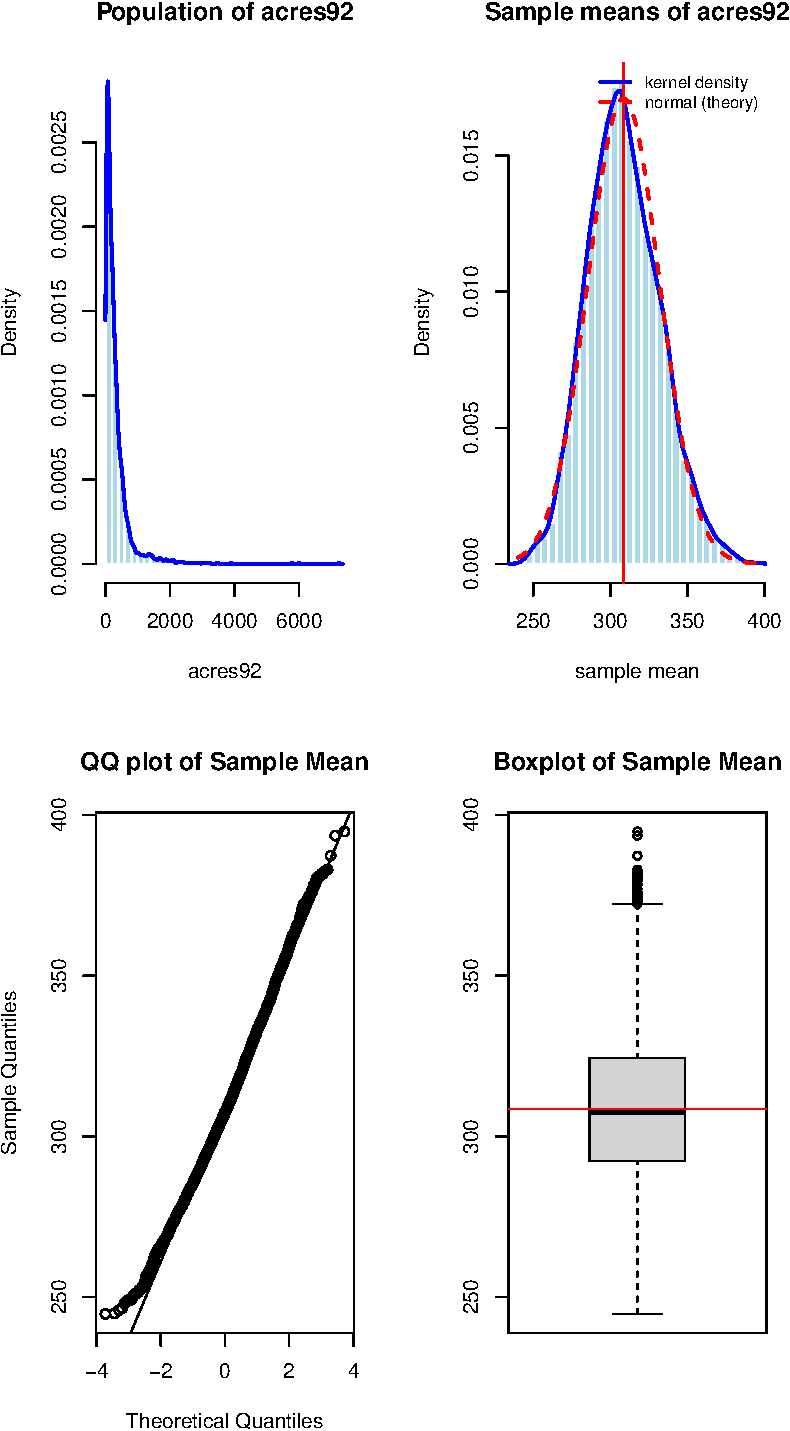
\includegraphics[keepaspectratio]{srs_files/figure-pdf/fig-srs-simulation-distribution-1.pdf}}

}

\caption{\label{fig-srs-simulation-distribution}Population distribution
and sampling distribution of the SRS sample mean over 5000 repeated
samples (n = 300)}

\end{figure}%

The blue curves are kernel density estimates. The population density
(top left) is strongly skewed to the right, with a long tail of very
large counties. The kernel density of the 5000 sample means (top right)
is nearly symmetric and almost coincides with the normal density
\(N\big(\bar y_U,\ \mathrm{SD}(\bar y)^2\big)\) predicted by the theory
(red dashed curve); the QQ plot (bottom left) is close to a straight
line, with only a slight bend in the upper tail left over from the
skewness. So the sampling distribution of \(\bar y\) is close to normal,
as Hájek's theorem and the \(n_{\min}\) check of
Section~\ref{sec-srs-ci} suggest. The average of the 5000 estimates,
308.76, is close to \(\bar y_U = 308.58\) (unbiasedness), and their
standard deviation, 23.42, is close to the theoretical value 23.32.

\subsection{Empirical coverage rate of
CIs}\label{empirical-coverage-rate-of-cis}

Finally we check whether the 95\% CIs cover the true mean about 95\% of
the time.

\begin{Shaded}
\begin{Highlighting}[]
\FunctionTok{library}\NormalTok{(plotrix)}

\CommentTok{\# Convert to data frame (if it was a matrix) and use mutate to evaluate coverage}
\NormalTok{simulation.results }\OtherTok{\textless{}{-}} \FunctionTok{as.data.frame}\NormalTok{(simulation.results) }\SpecialCharTok{|\textgreater{}}
  \FunctionTok{mutate}\NormalTok{(}
    \StringTok{\textasciigrave{}}\AttributeTok{Covered?}\StringTok{\textasciigrave{}} \OtherTok{=} \FunctionTok{as.numeric}\NormalTok{(ci.low }\SpecialCharTok{\textless{}}\NormalTok{ ybarU }\SpecialCharTok{\&}\NormalTok{ ybarU }\SpecialCharTok{\textless{}}\NormalTok{ ci.upp)}
\NormalTok{  )}

\FunctionTok{head}\NormalTok{(simulation.results)}
\end{Highlighting}
\end{Shaded}

\begin{verbatim}
      Est.     S.E.   ci.low   ci.upp Covered?
1 279.7295 17.80446 244.6916 314.7674        1
2 298.6389 21.71196 255.9113 341.3665        1
3 297.2253 20.55610 256.7723 337.6782        1
4 300.1009 22.33300 256.1511 344.0507        1
5 320.6076 27.30365 266.8760 374.3393        1
6 337.7321 31.58475 275.5755 399.8887        1
\end{verbatim}

\begin{Shaded}
\begin{Highlighting}[]
\FunctionTok{par}\NormalTok{(}\AttributeTok{mfrow=}\FunctionTok{c}\NormalTok{(}\DecValTok{1}\NormalTok{,}\DecValTok{1}\NormalTok{))}
\FunctionTok{plotCI}\NormalTok{(}
  \AttributeTok{x =} \DecValTok{1}\SpecialCharTok{:}\DecValTok{100}\NormalTok{,}
  \AttributeTok{y =}\NormalTok{ simulation.results}\SpecialCharTok{$}\NormalTok{Est.[}\DecValTok{1}\SpecialCharTok{:}\DecValTok{100}\NormalTok{],}
  \AttributeTok{li =}\NormalTok{ simulation.results}\SpecialCharTok{$}\NormalTok{ci.low[}\DecValTok{1}\SpecialCharTok{:}\DecValTok{100}\NormalTok{],}
  \AttributeTok{ui =}\NormalTok{ simulation.results}\SpecialCharTok{$}\NormalTok{ci.upp[}\DecValTok{1}\SpecialCharTok{:}\DecValTok{100}\NormalTok{],}
  \AttributeTok{col =} \DecValTok{2} \SpecialCharTok{{-}}\NormalTok{ simulation.results}\SpecialCharTok{$}\StringTok{\textasciigrave{}}\AttributeTok{Covered?}\StringTok{\textasciigrave{}}\NormalTok{[}\DecValTok{1}\SpecialCharTok{:}\DecValTok{100}\NormalTok{]}
\NormalTok{)}
\FunctionTok{abline}\NormalTok{(}\AttributeTok{h =}\NormalTok{ ybarU, }\AttributeTok{col =} \StringTok{"blue"}\NormalTok{)}

\CommentTok{\# Empirical coverage rate}
\FunctionTok{mean}\NormalTok{(simulation.results}\SpecialCharTok{$}\StringTok{\textasciigrave{}}\AttributeTok{Covered?}\StringTok{\textasciigrave{}}\NormalTok{)}
\end{Highlighting}
\end{Shaded}

\begin{verbatim}
[1] 0.9358
\end{verbatim}

\begin{figure}[H]

\centering{

\pandocbounded{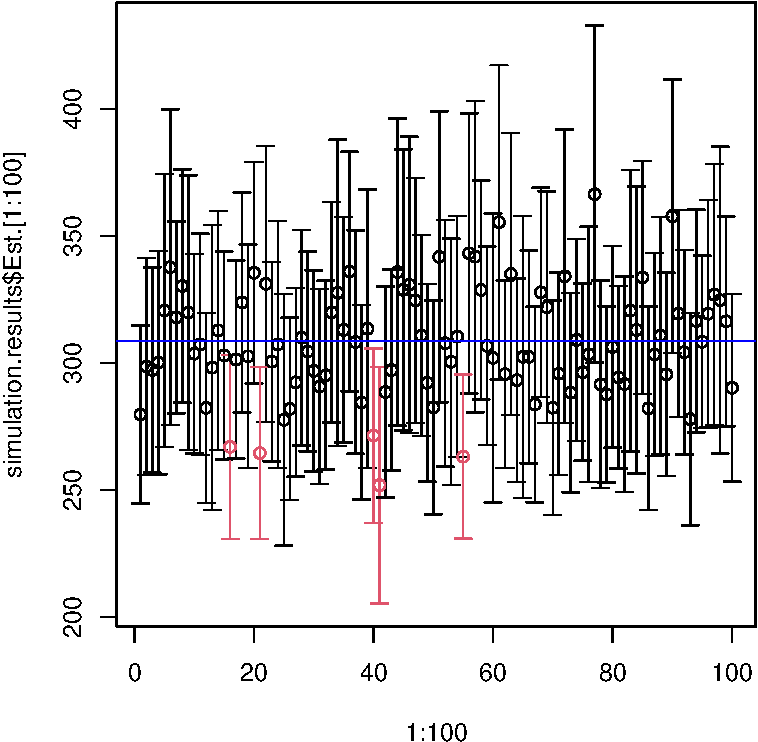
\includegraphics[keepaspectratio]{srs_files/figure-pdf/fig-srs-coverage-intervals-1.pdf}}

}

\caption{\label{fig-srs-coverage-intervals}First 100 simulated 95\%
confidence intervals for the SRS sample mean, with coverage failures
highlighted}

\end{figure}%

The empirical coverage rate is 0.936, close to the nominal 0.95. (With a
skewed population the coverage of the \(t\) interval tends to fall
slightly short of nominal.) The intervals that miss (in red) are exactly
the ``5\% of samples'' in the heuristic interpretation of
Section~\ref{sec-srs-ci}.

\section{Shinylive App for Illustrating SRS Theory}\label{sec-app-srs}

The simulation for this section runs as a standalone app:
\href{../shinylives_sampling/app-srs.html}{Simple random sampling}. It
draws samples one at a time and builds up the sampling distribution and
the coverage rate interactively, for any sample size and confidence
level. It opens in a new tab, together with its documentation and the
full \href{../shinylives_sampling/index.html}{list of apps}.

\bookmarksetup{startatroot}

\chapter{Stratified Random Sampling}\label{stratified-random-sampling}

\section{What Is Stratified Sampling?}\label{sec-strata-intro}

Suppose the variable we are interested in has different means in
different subpopulations. Then a stratified random sample can often give
more precise estimates of population quantities than a simple random
sample of the same size. The word \emph{stratify} comes from Latin words
meaning ``to make layers''. We divide the population of \(N\) units into
\(H\) subpopulations, called \textbf{strata}. The strata do not overlap
and together they make up the whole population, so each sampling unit
belongs to exactly one stratum. We then draw an independent probability
sample from each stratum and pool the information to estimate population
quantities.

Figure~\ref{fig-strata-pop} illustrates the design on a synthetic
population of \(N = 1000\) units in \(H = 4\) strata of sizes
\(N_h = 400, 300, 200\) and \(100\), sorted by their means. The sample
of \(n = 60\) is allocated in proportion to the stratum sizes,
\(n_h = 60 N_h/N = 24, 18, 12\) and \(6\), and an SRS of \(n_h\) units
is drawn in each stratum, so every stratum is represented in the sample.
Because the stratum means are far apart while the spread within each
stratum is small, most of the variation in the population lies
\emph{between} the strata, and this part of the variation does not
affect the stratified estimator (Section~\ref{sec-strata-estimation}).

\begin{figure}

\centering{

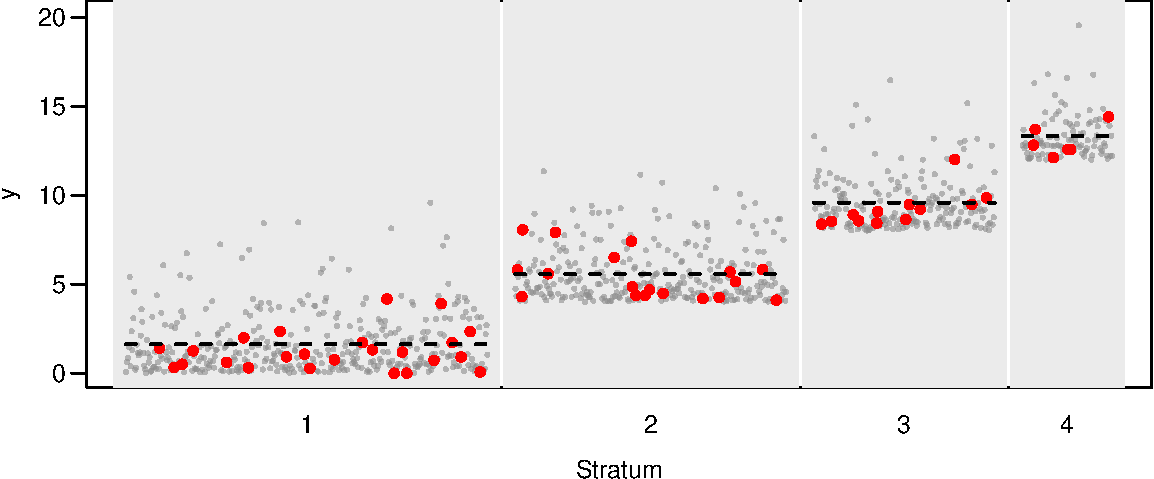
\includegraphics[width=0.85\linewidth,height=\textheight,keepaspectratio]{strata_files/figure-pdf/fig-strata-pop-1.pdf}

}

\caption{\label{fig-strata-pop}A stratified random sample from a
synthetic population of \(N = 1000\) units in \(H = 4\) strata of sizes
\(N_h = 400, 300, 200, 100\), sorted by their means (dashed lines). An
SRS of \(n_h = 24, 18, 12, 6\) units (red) is drawn in each stratum
(proportional allocation).}

\end{figure}%

In this chapter the sample within each stratum is a simple random sample
(SRS), drawn without replacement. The design is then called
\textbf{stratified random sampling}. The material corresponds to
Sections 3.1--3.5 of Lohr and Sections 5.1--5.9 of Scheaffer et al.

\textbf{Example: stratifying U.S. counties by census region.} In the SRS
chapter we sampled about 10\% of the 3078 U.S. counties to estimate the
average farm acreage per county. Here we use the four U.S. census
regions as strata. To compare stratified sampling directly with SRS, we
again sample about 10\% of the counties, this time 10\% of the counties
in \emph{each} stratum:

{\def\LTcaptype{none} % do not increment counter
\begin{longtable}[]{@{}lrr@{}}
\toprule\noalign{}
Stratum & Counties in stratum (\(N_h\)) & Counties in sample
(\(n_h\)) \\
\midrule\noalign{}
\endhead
\bottomrule\noalign{}
\endlastfoot
Northeast & 220 & 21 \\
North Central & 1054 & 103 \\
South & 1382 & 135 \\
West & 422 & 41 \\
\textbf{Total} & \textbf{3078} & \textbf{300} \\
\end{longtable}
}

We select four separate, independent SRSs, one per stratum. Knowing
which counties are in the sample from the Northeast tells us nothing
about which counties are in the sample from the South. We analyze these
data in Section~\ref{sec-strata-agstrat}.

\section{Estimation with Stratified
Samples}\label{sec-strata-estimation}

\subsection{Population quantities}\label{population-quantities-1}

Let \(y_{hj}\) be the value of unit \(j\) in stratum \(h\), for
\(j = 1, \ldots, N_h\) and \(h = 1, \ldots, H\), so that
\(N = \sum_{h=1}^H N_h\). The \textbf{stratum weight} \[
\pi_h = \frac{N_h}{N}
\] is the proportion of population units in stratum \(h\), so
\(\sum_{h=1}^H \pi_h = 1\). The population quantities of each stratum,
and of the whole population, are \[
t_h = \sum_{j=1}^{N_h} y_{hj} \quad(\text{stratum total}), \qquad
t = \sum_{h=1}^H t_h \quad(\text{population total}),
\] \[
\overline y_{hU} = \frac{t_h}{N_h} \quad(\text{stratum mean}), \qquad
\overline y_U = \frac tN = \sum_{h=1}^H \pi_h\, \overline y_{hU} \quad(\text{overall mean}),
\] \[
S_h^2 = \frac{1}{N_h-1}\sum_{j=1}^{N_h}(y_{hj}-\overline y_{hU})^2 \quad(\text{stratum variance}).
\] The overall mean \(\overline y_U\) is the average of the stratum
means, weighted by the stratum weights.

\subsection{SRS estimators within each
stratum}\label{srs-estimators-within-each-stratum}

Let \(\mathcal S_h\) be the SRS of \(n_h\) units drawn from stratum
\(h\), with total sample size \(n = \sum_{h=1}^H n_h\). Within stratum
\(h\) we have an ordinary SRS, so we estimate the stratum quantities
with the SRS formulas, applied separately to each stratum: \[
\overline y_h = \frac{1}{n_h}\sum_{j\in\mathcal S_h} y_{hj}, \qquad
\hat t_h = \frac{N_h}{n_h}\sum_{j\in\mathcal S_h} y_{hj} = N_h \overline y_h, \qquad
s_h^2 = \frac{1}{n_h - 1}\sum_{j\in\mathcal S_h} (y_{hj}-\overline y_h)^2 .
\]

\subsection{Estimators for the population total and
mean}\label{estimators-for-the-population-total-and-mean}

Adding up the estimated stratum totals gives the stratified estimator of
the population total. Dividing it by \(N\) gives the estimator of the
population mean: \[
\boxed{
\hat t_{\text{str}} = \sum_{h=1}^H \hat t_h = \sum_{h=1}^H N_h \overline y_h,
\qquad
\overline y_{\text{str}} = \frac{\hat t_{\text{str}}}{N} = \sum_{h=1}^H \pi_h\overline y_h .}
\] So \(\overline y_{\text{str}}\) is a weighted average of the stratum
sample means, with \(\overline y_h\) weighted by \(\pi_h = N_h/N\), the
fraction of population units in stratum \(h\). To use stratified
sampling, the stratum sizes \(N_h\) must be known.

\textbf{Unbiasedness.} Since an SRS is taken in each stratum,
\(E[\overline y_h]=\overline y_{hU}\). Averaging these unbiased stratum
estimates with the fixed weights \(N_h/N\) keeps the overall estimate
unbiased: \[
E[\overline y_{\text{str}}]
 = \sum_{h=1}^H \frac{N_h}{N}E[\overline y_h]
 = \sum_{h=1}^H \frac{N_h}{N}\cdot \frac{1}{N_h}\sum_{j=1}^{N_h} y_{hj}
 = \frac1N\sum_{h=1}^H \sum_{j=1}^{N_h}y_{hj} = \overline y_U .
\] It follows that \(E[\hat t_{\text{str}}] = N\,\overline y_U = t\).

\subsection{Variances and standard
errors}\label{variances-and-standard-errors}

The strata are sampled independently, so the \(\hat t_h\) are
independent and their variances add. Each \(\hat t_h\) has the SRS
variance \(N_h^2(1-n_h/N_h)S_h^2/n_h\), so \[
V(\hat t_{\text{str}}) = \sum_{h=1}^H V(\hat t_h) = \sum_{h=1}^H \Big(1-\frac{n_h}{N_h}\Big)N_h^2\frac{S_h^2}{n_h},
\qquad
V(\overline y_{\text{str}}) = \frac{V(\hat t_{\text{str}})}{N^2} = \sum_{h=1}^H \Big(1-\frac{n_h}{N_h}\Big)\pi_h^2 \frac{S_h^2}{n_h}.
\] Only the variability \emph{within} the strata enters these variances.
The differences \emph{between} the stratum means do not. This is the
source of the gain from stratification: if the strata are internally
homogeneous, every \(S_h^2\) is small, even when the population as a
whole is very variable.

Substituting the sample variances \(s_h^2\) for \(S_h^2\) gives unbiased
variance estimators, and their square roots are the standard errors: \[
\boxed{
\hat V(\overline y_{\text{str}}) = \sum_{h=1}^H v_h, \qquad
v_h = \Big(1-\frac{n_h}{N_h}\Big)\pi_h^2\frac{s_h^2}{n_h}, \qquad
\mathrm{SE}(\overline y_{\text{str}}) = \sqrt{\hat V(\overline y_{\text{str}})} ,}
\] \[
\hat V(\hat t_{\text{str}}) = N^2\,\hat V(\overline y_{\text{str}}) = \sum_{h=1}^H \Big(1-\frac{n_h}{N_h}\Big)N_h^2\frac{s_h^2}{n_h},
\qquad
\mathrm{SE}(\hat t_{\text{str}}) = N\,\mathrm{SE}(\overline y_{\text{str}}).
\] Here \(v_h\) is the contribution of stratum \(h\) to the estimated
variance. It appears as the last column of the working tables in this
chapter. Each stratum needs at least two sampled units, \(n_h \ge 2\),
so that \(s_h^2\) can be computed.

\subsection{Confidence intervals}\label{confidence-intervals}

Suppose either the sample sizes within the strata are large, or the
design has a large number of strata. Then \(\overline y_{\text{str}}\)
is approximately normal, and an approximate \(100(1-\alpha)\%\)
confidence interval for \(\overline y_U\) is \[
\overline y_{\text{str}} \pm z_{\alpha/2}\,\mathrm{SE}(\overline y_{\text{str}}).
\] When \(n\) is not large, it is common to replace the normal quantile
by the quantile of a \(t\) distribution with \(n-H\) degrees of freedom,
for example
\(\hat t_{\text{str}} \pm t_{\alpha/2,\,n-H}\,\mathrm{SE}(\hat t_{\text{str}})\)
for the total. The functions used in this book use \(z_{0.025} = 1.96\).

\section{Example: The Nelchina Caribou Herd}\label{sec-strata-caribou}

Siniff and Skoog (1964) used stratified random sampling to estimate the
size of the Nelchina herd of Alaska caribou in February 1962.
Preliminary estimates of caribou density were used to divide the area of
interest into six strata. Each stratum was divided into a grid of
4-mi\(^2\) sampling units. Stratum A, for example, contained \(N_1=400\)
sampling units, of which \(n_1=98\) were randomly selected for the
survey. Figure~\ref{fig-caribou-strata} shows the layout.

\begin{figure}

\centering{

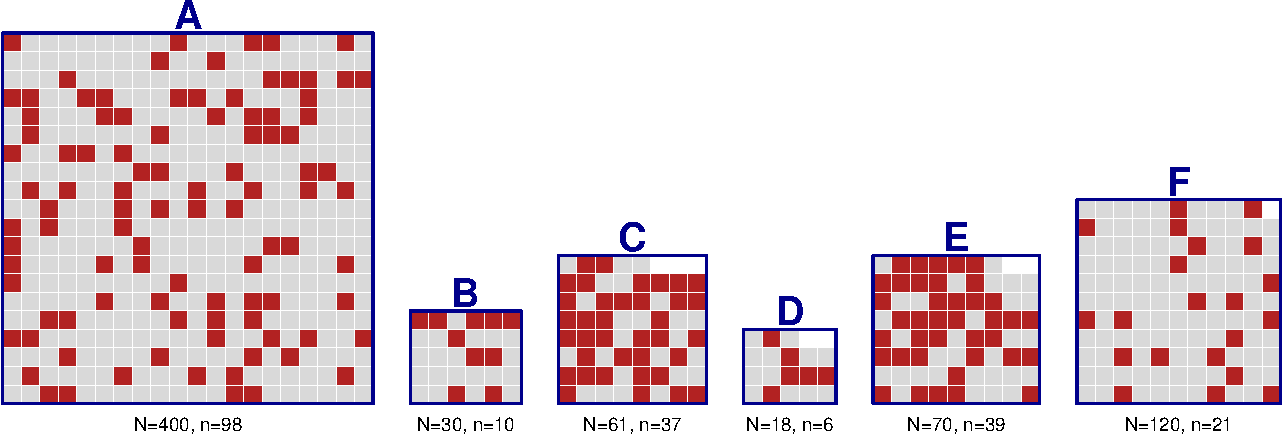
\includegraphics[width=0.95\linewidth,height=\textheight,keepaspectratio]{strata_files/figure-pdf/fig-caribou-strata-1.pdf}

}

\caption{\label{fig-caribou-strata}The six caribou strata. Each grid
holds one stratum's \(N_h\) sampling units; the red cells are the
\(n_h\) units selected at random in that stratum.}

\end{figure}%

\textbf{Spreadsheet calculation.} The survey gives the sample mean
\(\overline y_h\) and the sample variance \(s_h^2\) of the caribou
counts in each stratum. With \(N = 699\), the calculation fits in a
spreadsheet. The column \(\pi_h \overline y_h\) holds each stratum's
contribution to \(\overline y_{\text{str}}=\sum_h \pi_h\overline y_h\).
The column
\(v_h = \big(1-\tfrac{n_h}{N_h}\big)\pi_h^2\tfrac{s_h^2}{n_h}\) holds
its contribution to \(\hat V(\overline y_{\text{str}}) = \sum_h v_h\):

{\def\LTcaptype{none} % do not increment counter
\begin{longtable}[]{@{}
  >{\centering\arraybackslash}p{(\linewidth - 14\tabcolsep) * \real{0.1351}}
  >{\raggedleft\arraybackslash}p{(\linewidth - 14\tabcolsep) * \real{0.1081}}
  >{\raggedleft\arraybackslash}p{(\linewidth - 14\tabcolsep) * \real{0.1081}}
  >{\raggedleft\arraybackslash}p{(\linewidth - 14\tabcolsep) * \real{0.2162}}
  >{\raggedleft\arraybackslash}p{(\linewidth - 14\tabcolsep) * \real{0.1081}}
  >{\raggedleft\arraybackslash}p{(\linewidth - 14\tabcolsep) * \real{0.1081}}
  >{\raggedleft\arraybackslash}p{(\linewidth - 14\tabcolsep) * \real{0.1081}}
  >{\raggedleft\arraybackslash}p{(\linewidth - 14\tabcolsep) * \real{0.1081}}@{}}
\toprule\noalign{}
\begin{minipage}[b]{\linewidth}\centering
Stratum
\end{minipage} & \begin{minipage}[b]{\linewidth}\raggedleft
\(N_h\)
\end{minipage} & \begin{minipage}[b]{\linewidth}\raggedleft
\(n_h\)
\end{minipage} & \begin{minipage}[b]{\linewidth}\raggedleft
\(\pi_h=N_h/N\)
\end{minipage} & \begin{minipage}[b]{\linewidth}\raggedleft
\(\overline y_h\)
\end{minipage} & \begin{minipage}[b]{\linewidth}\raggedleft
\(s_h^2\)
\end{minipage} & \begin{minipage}[b]{\linewidth}\raggedleft
\(\pi_h\overline y_h\)
\end{minipage} & \begin{minipage}[b]{\linewidth}\raggedleft
\(v_h\)
\end{minipage} \\
\midrule\noalign{}
\endhead
\bottomrule\noalign{}
\endlastfoot
A & 400 & 98 & 0.5722 & 24.1 & 5,575 & 13.7911 & 14.0648 \\
B & 30 & 10 & 0.0429 & 25.6 & 4,064 & 1.0987 & 0.4991 \\
C & 61 & 37 & 0.0873 & 267.6 & 347,556 & 23.3528 & 28.1455 \\
D & 18 & 6 & 0.0258 & 179.0 & 22,798 & 4.6094 & 1.6798 \\
E & 70 & 39 & 0.1001 & 293.7 & 123,578 & 29.4120 & 14.0728 \\
F & 120 & 21 & 0.1717 & 33.2 & 9,795 & 5.6996 & 11.3409 \\
\textbf{Total} & \textbf{699} & \textbf{211} & \textbf{1.0000} & & &
\textbf{77.9636} & \textbf{69.8029} \\
\end{longtable}
}

\textbf{Results.} The estimated mean number of caribou per sampling
unit, and its standard error, are \[
\overline y_{\text{str}} = 77.96, \qquad \mathrm{SE}(\overline y_{\text{str}}) = \sqrt{69.8029} = 8.35 .
\] Multiplying by \(N = 699\) gives the estimated total number of
caribou: \[
\hat t_{\text{str}} = 699(77.96) = 54{,}497, \qquad
\mathrm{SE}(\hat t_{\text{str}}) = 699(8.35) = 5{,}840,
\] and an approximate 95\% confidence interval for the size of the herd
is \[
54{,}497 \pm 1.96(5{,}840) = [43{,}051,\ 65{,}943].
\] This interval reflects only sampling error. If the field procedure
for counting caribou tends to miss animals, the whole interval will be
biased low.

Strata C and E have far fewer units than stratum A, yet they contribute
most of the estimate and much of its variance. These are the
high-density strata, where the caribou counts are large and highly
variable. We return to this point when we discuss optimal allocation in
Section~\ref{sec-strata-optimal}.

\textbf{The same calculation in R.} The function \texttt{str\_est()}
from the shared file \texttt{samplingestimate.r} (see
Section~\ref{sec-strata-functions}) takes the stratum summaries
\(\overline y_h\), \(s_h\), \(n_h\) and \(N_h\) and produces the same
working table:

\begin{Shaded}
\begin{Highlighting}[]
\NormalTok{Nh }\OtherTok{\textless{}{-}} \FunctionTok{c}\NormalTok{(}\AttributeTok{A =} \DecValTok{400}\NormalTok{, }\AttributeTok{B =} \DecValTok{30}\NormalTok{, }\AttributeTok{C =} \DecValTok{61}\NormalTok{, }\AttributeTok{D =} \DecValTok{18}\NormalTok{, }\AttributeTok{E =} \DecValTok{70}\NormalTok{, }\AttributeTok{F =} \DecValTok{120}\NormalTok{)}
\NormalTok{nh }\OtherTok{\textless{}{-}} \FunctionTok{c}\NormalTok{(}\DecValTok{98}\NormalTok{, }\DecValTok{10}\NormalTok{, }\DecValTok{37}\NormalTok{, }\DecValTok{6}\NormalTok{, }\DecValTok{39}\NormalTok{, }\DecValTok{21}\NormalTok{)}
\NormalTok{ybarh }\OtherTok{\textless{}{-}} \FunctionTok{c}\NormalTok{(}\FloatTok{24.1}\NormalTok{, }\FloatTok{25.6}\NormalTok{, }\FloatTok{267.6}\NormalTok{, }\FloatTok{179.0}\NormalTok{, }\FloatTok{293.7}\NormalTok{, }\FloatTok{33.2}\NormalTok{)}
\NormalTok{s2h }\OtherTok{\textless{}{-}} \FunctionTok{c}\NormalTok{(}\DecValTok{5575}\NormalTok{, }\DecValTok{4064}\NormalTok{, }\DecValTok{347556}\NormalTok{, }\DecValTok{22798}\NormalTok{, }\DecValTok{123578}\NormalTok{, }\DecValTok{9795}\NormalTok{)}

\NormalTok{res\_caribou }\OtherTok{\textless{}{-}} \FunctionTok{str\_est}\NormalTok{(ybarh, }\FunctionTok{sqrt}\NormalTok{(s2h), nh, Nh, }\AttributeTok{estimate =} \StringTok{"mean"}\NormalTok{)}
\NormalTok{res\_caribou}\SpecialCharTok{$}\NormalTok{table}
\end{Highlighting}
\end{Shaded}

\begin{table}[H]
\caption*{
{\large  Stratified Mean Estimation: Working Table\normalsize }
} 
\normalsize
\begin{gtfit}{\linewidth}{>{\raggedright\arraybackslash}p{\dimexpr 82.50pt -2\tabcolsep-1.5\arrayrulewidth}>{\raggedleft\arraybackslash}p{\dimexpr 45.00pt -2\tabcolsep-1.5\arrayrulewidth}>{\raggedleft\arraybackslash}p{\dimexpr 45.00pt -2\tabcolsep-1.5\arrayrulewidth}>{\raggedleft\arraybackslash}p{\dimexpr 82.50pt -2\tabcolsep-1.5\arrayrulewidth}>{\raggedleft\arraybackslash}p{\dimexpr 82.50pt -2\tabcolsep-1.5\arrayrulewidth}>{\raggedleft\arraybackslash}p{\dimexpr 82.50pt -2\tabcolsep-1.5\arrayrulewidth}>{\raggedleft\arraybackslash}p{\dimexpr 82.50pt -2\tabcolsep-1.5\arrayrulewidth}>{\raggedleft\arraybackslash}p{\dimexpr 82.50pt -2\tabcolsep-1.5\arrayrulewidth}}
\toprule
Stratum & \(N_h\) & \(n_h\) & \(\pi_h\)\textsuperscript{\textit{1}} & \(\bar y_h\) & \(s_h^2\) & \(\pi_h\bar y_h\) & \(v_h\)\textsuperscript{\textit{2}} \\ 
\midrule\addlinespace[2.5pt]
A & 400 & 98 & 0.57 & 24.10 & 5,575.00 & 13.79 & 14.06 \\ 
B & 30 & 10 & 0.04 & 25.60 & 4,064.00 & 1.10 & 0.50 \\ 
C & 61 & 37 & 0.09 & 267.60 & 347,556.00 & 23.35 & 28.15 \\ 
D & 18 & 6 & 0.03 & 179.00 & 22,798.00 & 4.61 & 1.68 \\ 
E & 70 & 39 & 0.10 & 293.70 & 123,578.00 & 29.41 & 14.07 \\ 
F & 120 & 21 & 0.17 & 33.20 & 9,795.00 & 5.70 & 11.34 \\ 
{\bfseries Total} & {\bfseries 699} & {\bfseries 211} & {\bfseries 1.00} & {\bfseries } & {\bfseries } & {\bfseries 77.96} & {\bfseries 69.80} \\ 
\bottomrule
\end{gtfit}
\begin{minipage}{\linewidth}
\vspace{.05em}
\textsuperscript{\textit{1}}\(\pi_h = N_h/N\) is the stratum weight.\\
\textsuperscript{\textit{2}}\(v_h = (1-n_h/N_h)\,\pi_h^2\, s_h^2/n_h\) is stratum \(h\)'s contribution to \(V(\bar y_{str}) = \sum_h v_h\).\\
\(\bar y_{str} = \sum_h \pi_h\bar y_h = 77.96\)\\
\(\mathrm{SE}(\bar y_{str}) = \sqrt{\sum_h v_h} = \sqrt{69.80} = 8.35\)\\
\end{minipage}
\end{table}

\begin{Shaded}
\begin{Highlighting}[]
\FunctionTok{str\_est}\NormalTok{(ybarh, }\FunctionTok{sqrt}\NormalTok{(s2h), nh, Nh, }\AttributeTok{estimate =} \StringTok{"total"}\NormalTok{)}\SpecialCharTok{$}\NormalTok{estimate }\SpecialCharTok{|\textgreater{}} \FunctionTok{format\_est\_gt}\NormalTok{(}\StringTok{"total"}\NormalTok{)}
\end{Highlighting}
\end{Shaded}

\begin{table}[H]
\normalsize
\begin{gtfit}{0.7\linewidth}{rrrr}
\toprule
\(\hat{t}\) & \(\mathrm{SE}(\hat{t})\) & 95\% CI Lower & 95\% CI Upper \\ 
\midrule\addlinespace[2.5pt]
54,496.60 & 5,840.01 & 43,050.18 & 65,943.02 \\ 
\bottomrule
\end{gtfit}
\end{table}

\section{Stratified Sampling for
Proportions}\label{sec-strata-proportions}

A proportion is the mean of a 0/1 variable. So we can apply the same
formulas with \(\overline y_h = \hat p_h\), the sample proportion in
stratum \(h\), and \(s_h^2 = \frac{n_h}{n_h-1}\hat p_h(1-\hat p_h)\): \[
\boxed{\hat p_{\text{str}} = \sum_{h=1}^H \frac{N_h}{N}\hat p_h, \qquad
\hat V(\hat p_{\text{str}}) = \sum_{h=1}^H \Big(1-\frac{n_h}{N_h}\Big)\Big(\frac{N_h}{N}\Big)^2\frac{\hat p_h(1-\hat p_h)}{n_h-1}}.
\] The total number of units with the attribute is estimated by
\(N\hat p_{\text{str}}\), with standard error
\(N\,\mathrm{SE}(\hat p_{\text{str}})\).

\textbf{Example: ACLS survey of scholars.} The American Council of
Learned Societies (ACLS) used a stratified random sample of the members
of seven disciplinary societies. It studied publication patterns and the
use of computers and libraries (Morton and Price, 1989). The membership
figures \(N_h\), the numbers of valid returns \(n_h\), and the
percentage of female respondents were:

{\def\LTcaptype{none} % do not increment counter
\begin{longtable}[]{@{}
  >{\raggedright\arraybackslash}p{(\linewidth - 6\tabcolsep) * \real{0.2500}}
  >{\raggedleft\arraybackslash}p{(\linewidth - 6\tabcolsep) * \real{0.2500}}
  >{\raggedleft\arraybackslash}p{(\linewidth - 6\tabcolsep) * \real{0.2500}}
  >{\raggedleft\arraybackslash}p{(\linewidth - 6\tabcolsep) * \real{0.2500}}@{}}
\toprule\noalign{}
\begin{minipage}[b]{\linewidth}\raggedright
Discipline
\end{minipage} & \begin{minipage}[b]{\linewidth}\raggedleft
Membership (\(N_h\))
\end{minipage} & \begin{minipage}[b]{\linewidth}\raggedleft
Valid returns (\(n_h\))
\end{minipage} & \begin{minipage}[b]{\linewidth}\raggedleft
Female members (\%)
\end{minipage} \\
\midrule\noalign{}
\endhead
\bottomrule\noalign{}
\endlastfoot
Literature & 9,100 & 636 & 38 \\
Classics & 1,950 & 451 & 27 \\
Philosophy & 5,500 & 481 & 18 \\
History & 10,850 & 611 & 19 \\
Linguistics & 2,100 & 493 & 36 \\
Political Science & 5,500 & 575 & 13 \\
Sociology & 9,000 & 588 & 26 \\
\textbf{Totals} & \textbf{44,000} & \textbf{3,835} & \\
\end{longtable}
}

We estimate the proportion of these scholars who are female, ignoring
nonresponse for now. With \(N = 44{,}000\), the spreadsheet calculation
is:

{\def\LTcaptype{none} % do not increment counter
\begin{longtable}[]{@{}
  >{\raggedright\arraybackslash}p{(\linewidth - 12\tabcolsep) * \real{0.1212}}
  >{\raggedleft\arraybackslash}p{(\linewidth - 12\tabcolsep) * \real{0.1212}}
  >{\raggedleft\arraybackslash}p{(\linewidth - 12\tabcolsep) * \real{0.1212}}
  >{\raggedleft\arraybackslash}p{(\linewidth - 12\tabcolsep) * \real{0.2121}}
  >{\raggedleft\arraybackslash}p{(\linewidth - 12\tabcolsep) * \real{0.1212}}
  >{\raggedleft\arraybackslash}p{(\linewidth - 12\tabcolsep) * \real{0.1212}}
  >{\raggedleft\arraybackslash}p{(\linewidth - 12\tabcolsep) * \real{0.1818}}@{}}
\toprule\noalign{}
\begin{minipage}[b]{\linewidth}\raggedright
Discipline
\end{minipage} & \begin{minipage}[b]{\linewidth}\raggedleft
\(N_h\)
\end{minipage} & \begin{minipage}[b]{\linewidth}\raggedleft
\(n_h\)
\end{minipage} & \begin{minipage}[b]{\linewidth}\raggedleft
\(\pi_h=N_h/N\)
\end{minipage} & \begin{minipage}[b]{\linewidth}\raggedleft
\(\hat p_h\)
\end{minipage} & \begin{minipage}[b]{\linewidth}\raggedleft
\(\pi_h\hat p_h\)
\end{minipage} & \begin{minipage}[b]{\linewidth}\raggedleft
\(v_h\) (\(\times10^{-5}\))
\end{minipage} \\
\midrule\noalign{}
\endhead
\bottomrule\noalign{}
\endlastfoot
Literature & 9,100 & 636 & 0.2068 & 0.38 & 0.0786 & 1.476 \\
Classics & 1,950 & 451 & 0.0443 & 0.27 & 0.0120 & 0.066 \\
Philosophy & 5,500 & 481 & 0.1250 & 0.18 & 0.0225 & 0.439 \\
History & 10,850 & 611 & 0.2466 & 0.19 & 0.0469 & 1.448 \\
Linguistics & 2,100 & 493 & 0.0477 & 0.36 & 0.0172 & 0.082 \\
Political Science & 5,500 & 575 & 0.1250 & 0.13 & 0.0163 & 0.276 \\
Sociology & 9,000 & 588 & 0.2045 & 0.26 & 0.0532 & 1.282 \\
\textbf{Total} & \textbf{44,000} & \textbf{3,835} & \textbf{1.0000} & &
\textbf{0.2465} & \textbf{5.068} \\
\end{longtable}
}

Here
\(v_h = \big(1-\tfrac{n_h}{N_h}\big)\pi_h^2\tfrac{\hat p_h(1-\hat p_h)}{n_h-1}\).
Summing the columns gives \[
\hat p_{\text{str}} = \frac{9100}{44{,}000}(0.38) + \cdots + \frac{9000}{44{,}000}(0.26) = 0.2465,
\qquad
\mathrm{SE}(\hat p_{\text{str}}) = \sqrt{5.068\times10^{-5}} = 0.0071 .
\] About 24.7\% of the members are estimated to be female. To estimate
the total number of female scholars, multiply both numbers by
\(N = 44{,}000\). This gives about 10,846 women, with a standard error
of about 313.

In R, we pass \(s_h = \sqrt{n_h\hat p_h(1-\hat p_h)/(n_h-1)}\) to
\texttt{str\_est()}:

\begin{Shaded}
\begin{Highlighting}[]
\NormalTok{Nh }\OtherTok{\textless{}{-}} \FunctionTok{c}\NormalTok{(}\AttributeTok{Literature =} \DecValTok{9100}\NormalTok{, }\AttributeTok{Classics =} \DecValTok{1950}\NormalTok{, }\AttributeTok{Philosophy =} \DecValTok{5500}\NormalTok{, }\AttributeTok{History =} \DecValTok{10850}\NormalTok{,}
        \AttributeTok{Linguistics =} \DecValTok{2100}\NormalTok{, }\AttributeTok{PoliSci =} \DecValTok{5500}\NormalTok{, }\AttributeTok{Sociology =} \DecValTok{9000}\NormalTok{)}
\NormalTok{nh }\OtherTok{\textless{}{-}} \FunctionTok{c}\NormalTok{(}\DecValTok{636}\NormalTok{, }\DecValTok{451}\NormalTok{, }\DecValTok{481}\NormalTok{, }\DecValTok{611}\NormalTok{, }\DecValTok{493}\NormalTok{, }\DecValTok{575}\NormalTok{, }\DecValTok{588}\NormalTok{)}
\NormalTok{ph }\OtherTok{\textless{}{-}} \FunctionTok{c}\NormalTok{(}\FloatTok{0.38}\NormalTok{, }\FloatTok{0.27}\NormalTok{, }\FloatTok{0.18}\NormalTok{, }\FloatTok{0.19}\NormalTok{, }\FloatTok{0.36}\NormalTok{, }\FloatTok{0.13}\NormalTok{, }\FloatTok{0.26}\NormalTok{)}

\NormalTok{sh }\OtherTok{\textless{}{-}} \FunctionTok{sqrt}\NormalTok{(nh }\SpecialCharTok{/}\NormalTok{ (nh }\SpecialCharTok{{-}} \DecValTok{1}\NormalTok{) }\SpecialCharTok{*}\NormalTok{ ph }\SpecialCharTok{*}\NormalTok{ (}\DecValTok{1} \SpecialCharTok{{-}}\NormalTok{ ph))}
\FunctionTok{round}\NormalTok{(}\FunctionTok{str\_est}\NormalTok{(ph, sh, nh, Nh, }\AttributeTok{estimate =} \StringTok{"mean"}\NormalTok{, }\AttributeTok{show.details =} \ConstantTok{FALSE}\NormalTok{)}\SpecialCharTok{$}\NormalTok{estimate, }\DecValTok{4}\NormalTok{)}
\end{Highlighting}
\end{Shaded}

\begin{verbatim}
  Est.   S.E. ci.low ci.upp 
0.2465 0.0071 0.2326 0.2605 
\end{verbatim}

\section{\texorpdfstring{Alternative Formulas for
\(\overline y_{\text{str}}\)}{Alternative Formulas for \textbackslash overline y\_\{\textbackslash text\{str\}\}}}\label{sec-strata-alt-formulas}

The estimator \(\overline y_{\text{str}} = \sum_h \pi_h \overline y_h\)
can be written in two other ways. Each one shows something about the
design. The first compares it with the sample mean of an SRS and shows
why the weights must be \(N_h/N\). The second writes it as a weighted
average over individual units, with each unit weighted by its sampling
weight. This is the form used for survey data files.

\subsection{Weighting by population fractions instead of sample
fractions}\label{sec-strata-vs-srs-formulas}

Suppose instead that we had taken an SRS of size \(n=n_1+\cdots+n_H\)
from the whole population. Grouping the sampled units by stratum, the
sample mean is \[
\overline y_{\text{SRS}} = \frac{1}{n}\sum_{(h,j)\in\mathcal S} y_{hj}
 = \frac{n_1\overline y_1 + \cdots + n_H\overline y_H}{n}
 = \overline y_1\frac{n_1}{n} + \cdots + \overline y_H\frac{n_H}{n},
\] which we compare with the stratified estimator \[
\overline y_{\text{str}} = \overline y_1\frac{N_1}{N} + \cdots + \overline y_H\frac{N_H}{N}.
\] For proportions, similarly,
\(\hat p_{\text{SRS}} = \sum_{h} \frac{n_h}{n}\hat p_h\) while
\(\hat p_{\text{str}} = \sum_{h} \frac{N_h}{N}\hat p_h\).

Both estimators average the stratum sample means. The difference is in
the weights. In an SRS, the stratum sizes in the sample \(n_h\) are
random, so \(\overline y_{\text{SRS}}\) weights each stratum by its
\emph{realized} sample fraction \(n_h/n\). That fraction varies from
sample to sample and can be distorted by nonresponse rates that differ
between strata. In contrast, \(\overline y_{\text{str}}\) uses the
\emph{known, fixed} population fraction \(N_h/N\). These fixed weights
make it unbiased for \(\overline y_U\) whatever the \(n_h\) are. When
\(n_h/n = N_h/N\) for every \(h\) (proportional allocation,
Section~\ref{sec-strata-prop}), the two estimators coincide.

\subsection{Weighting each unit by its sampling
weight}\label{sec-strata-weights}

Write the stratified sample as
\(\mathcal S = (\mathcal S_1,\ldots,\mathcal S_H)\), where
\(\mathcal S_h\) is the SRS drawn from stratum \(h\). The strata are
sampled independently, so the probability of selecting a particular
sample is the product of the probabilities of its stratum samples: \[
P(\mathcal S) = P(\mathcal S_1)\times P(\mathcal S_2)\times\cdots\times P(\mathcal S_H)
 = \frac{1}{\binom{N_1}{n_1}}\cdot\frac{1}{\binom{N_2}{n_2}}\cdots\frac{1}{\binom{N_H}{n_H}}.
\]

For SRS we defined the sampling weight of a unit as the reciprocal of
its inclusion probability. A unit \(j\) in stratum \(h\) is included
with probability \(n_h/N_h\), the sampling fraction in stratum \(h\).
(Do not confuse this with the stratum weight \(\pi_h = N_h/N\).) So its
sampling weight is \[
w_{hj} = \frac{N_h}{n_h}.
\] Unless every stratum has the same sampling fraction, units in
different strata have different inclusion probabilities. Stratified
sampling is therefore an example of \textbf{unequal-probability
sampling}.

The sampling weight can be thought of as the number of population units
that a sampled unit represents. Within stratum \(h\) all \(n_h\) sampled
units have the same weight \(N_h/n_h\), so the weights add up to the
stratum sizes and to the population size: \[
\sum_{j\in\mathcal S_h} w_{hj} = n_h\cdot\frac{N_h}{n_h} = N_h,
\qquad
\sum_{h=1}^H\sum_{j\in\mathcal S_h} w_{hj} = \sum_{h=1}^H N_h = N.
\]

\textbf{Estimators in terms of the weights.} Since
\(N_h\overline y_h = \frac{N_h}{n_h}\sum_{j\in\mathcal S_h} y_{hj} = \sum_{j\in\mathcal S_h} w_{hj}\,y_{hj}\),
the estimated total is a weighted sum over \emph{all} sampled units,
regardless of stratum. Since the weights sum to \(N\), the estimated
mean is a weighted average: \[
\hat t_{\text{str}} = \sum_{h=1}^H \sum_{j\in\mathcal S_h} w_{hj}\, y_{hj},
\qquad
\overline y_{\text{str}} = \frac{\sum_{h=1}^H\sum_{j\in\mathcal S_h} w_{hj}y_{hj}}{\sum_{h=1}^H\sum_{j\in\mathcal S_h} w_{hj}}.
\] This is how survey data files are usually distributed: one row per
sampled unit, with a column of sampling weights. The \texttt{weight}
column of \texttt{agstrat.csv} in Section~\ref{sec-strata-agstrat} is an
example.

For the caribou survey the weights are:

{\def\LTcaptype{none} % do not increment counter
\begin{longtable}[]{@{}crrr@{}}
\toprule\noalign{}
Stratum & \(N_h\) & \(n_h\) & \(w_{hj} = N_h/n_h\) \\
\midrule\noalign{}
\endhead
\bottomrule\noalign{}
\endlastfoot
A & 400 & 98 & 4.08 \\
B & 30 & 10 & 3.00 \\
C & 61 & 37 & 1.65 \\
D & 18 & 6 & 3.00 \\
E & 70 & 39 & 1.79 \\
F & 120 & 21 & 5.71 \\
\end{longtable}
}

The weights alone are enough for the point estimates, but not for the
variances. Strata B and D have the same weight, so the weights do not
identify which stratum a unit belongs to. The variance estimator needs
\(s_h^2\) computed separately within each stratum, so the data file must
also record each unit's stratum.

\section{Analyzing Stratified Data in R}\label{sec-strata-functions}

The estimating functions used throughout this book live in a single
shared file, \texttt{samplingestimate.r}, sourced at the start of this
chapter. They include \texttt{str\_est}, \texttt{str\_est\_data} and
\texttt{srs\_est}, which compute the stratified mean, its standard error
and confidence intervals. \texttt{str\_est} works from the stratum
summaries (\(\overline y_h\), \(s_h\), \(n_h\), \(N_h\)), as in the
caribou example. \texttt{str\_est\_data} computes everything directly
from a data set with stratum and weight columns.

The full source of \texttt{samplingestimate.r} is listed in
Appendix~\ref{sec-estimating-functions}.

\subsection{Example: Farm acreage by census region
(agstrat.csv)}\label{sec-strata-agstrat}

We now analyze the stratified sample of counties described in
Section~\ref{sec-strata-intro}. The goal is to estimate the average 1992
farm acreage per county (\texttt{acres92}, in thousands of acres), with
the census region (\texttt{region}) as the stratification variable.

\begin{Shaded}
\begin{Highlighting}[]
\NormalTok{agstrat }\OtherTok{\textless{}{-}} \FunctionTok{acres\_in\_thousands}\NormalTok{(}\FunctionTok{read.csv}\NormalTok{(}\StringTok{"data/agstrat.csv"}\NormalTok{))}
\FunctionTok{head}\NormalTok{(agstrat) }\SpecialCharTok{|\textgreater{}} \FunctionTok{gt}\NormalTok{()}
\end{Highlighting}
\end{Shaded}

\begin{table}

\caption{\label{tbl-agstrat-sample-data}Sample survey data for
agstrat.csv, including stratum and weight}

\centering{

\normalsize
\begin{gtfit}{\linewidth}{llrrrrrrrrrrrrlrr}
\toprule
county & state & acres92 & acres87 & acres82 & farms92 & farms87 & farms82 & largef92 & largef87 & largef82 & smallf92 & smallf87 & smallf82 & region & rn & weight \\ 
\midrule\addlinespace[2.5pt]
PIERCE COUNTY & NE & 297.326 & 332.862 & 319.619 & 725 & 857 & 865 & 54 & 54 & 42 & 58 & 67 & 48 & NC & 805 & 10.23301 \\ 
JENNINGS COUNTY & IN & 124.694 & 131.481 & 139.111 & 658 & 671 & 751 & 14 & 13 & 14 & 42 & 36 & 38 & NC & 241 & 10.23301 \\ 
WAYNE COUNTY & OH & 246.938 & 263.457 & 268.434 & 1582 & 1734 & 1866 & 20 & 19 & 16 & 175 & 186 & 184 & NC & 913 & 10.23301 \\ 
VAN BUREN COUNTY & MI & 206.781 & 190.251 & 197.055 & 1164 & 1278 & 1464 & 23 & 17 & 9 & 56 & 66 & 55 & NC & 478 & 10.23301 \\ 
OZAUKEE COUNTY & WI & 78.772 & 85.201 & 89.331 & 448 & 483 & 527 & 6 & 5 & 5 & 56 & 49 & 48 & NC & 1028 & 10.23301 \\ 
CLEARWATER COUNTY & MN & 210.897 & 229.537 & 213.105 & 583 & 699 & 693 & 34 & 32 & 23 & 8 & 19 & 13 & NC & 496 & 10.23301 \\ 
\bottomrule
\end{gtfit}

}

\end{table}%

Each row is a sampled county. The column \texttt{region} is its stratum,
and \texttt{weight} is its sampling weight \(N_h/n_h\).

\subsubsection*{Summarizing acres92 in each
stratum}\label{summarizing-acres92-in-each-stratum}
\addcontentsline{toc}{subsubsection}{Summarizing acres92 in each
stratum}

We first compute the sample size (\(n_h\)), standard deviation (\(s_h\))
and mean (\(\overline{y}_h\)) for each region. These are matched with
the known numbers of counties in each region (\(N_h\)).

\begin{Shaded}
\begin{Highlighting}[]
\NormalTok{nh }\OtherTok{\textless{}{-}} \FunctionTok{tapply}\NormalTok{ (agstrat[, }\StringTok{"acres92"}\NormalTok{], agstrat[,}\StringTok{"region"}\NormalTok{], length)}
\NormalTok{sh }\OtherTok{\textless{}{-}} \FunctionTok{tapply}\NormalTok{ (agstrat[, }\StringTok{"acres92"}\NormalTok{], agstrat[,}\StringTok{"region"}\NormalTok{], sd)}
\NormalTok{ybarh }\OtherTok{\textless{}{-}} \FunctionTok{tapply}\NormalTok{ (agstrat[, }\StringTok{"acres92"}\NormalTok{], agstrat[,}\StringTok{"region"}\NormalTok{], mean)}
\CommentTok{\# create a vector with external information (true population size per stratum)}
\NormalTok{Nh }\OtherTok{\textless{}{-}} \FunctionTok{c}\NormalTok{(}\AttributeTok{NC =} \DecValTok{1054}\NormalTok{, }\AttributeTok{NE =} \DecValTok{220}\NormalTok{, }\AttributeTok{S=} \DecValTok{1382}\NormalTok{, }\AttributeTok{W =} \DecValTok{422}\NormalTok{)}

\FunctionTok{data.frame}\NormalTok{(Nh, nh, ybarh, sh) }\SpecialCharTok{|\textgreater{}}
  \FunctionTok{gt}\NormalTok{(}\AttributeTok{rownames\_to\_stub =} \ConstantTok{TRUE}\NormalTok{) }\SpecialCharTok{|\textgreater{}}
  \FunctionTok{cols\_label}\NormalTok{(}
    \AttributeTok{Nh =} \FunctionTok{md}\NormalTok{(}\StringTok{"$N\_h$"}\NormalTok{),}
    \AttributeTok{nh =} \FunctionTok{md}\NormalTok{(}\StringTok{"$n\_h$"}\NormalTok{),}
    \AttributeTok{ybarh =} \FunctionTok{md}\NormalTok{(}\StringTok{"$}\SpecialCharTok{\textbackslash{}\textbackslash{}}\StringTok{bar\{y\}\_h$"}\NormalTok{),}
    \AttributeTok{sh =} \FunctionTok{md}\NormalTok{(}\StringTok{"$s\_h$"}\NormalTok{)}
\NormalTok{  ) }\SpecialCharTok{|\textgreater{}}
  \FunctionTok{fmt\_number}\NormalTok{(}\AttributeTok{columns =} \FunctionTok{c}\NormalTok{(ybarh, sh), }\AttributeTok{decimals =} \DecValTok{2}\NormalTok{)}
\end{Highlighting}
\end{Shaded}

\begin{table}

\caption{\label{tbl-agstrat-summary-by-region}Sample summary statistics
for acres92 by region stratum}

\centering{

\normalsize
\begin{gtfit}{\linewidth}{l|rrrr}
\toprule
 & \(N_h\) & \(n_h\) & \(\bar{y}_h\) & \(s_h\) \\ 
\midrule\addlinespace[2.5pt]
NC & 1054 & 103 & 300.50 & 172.10 \\ 
NE & 220 & 21 & 97.63 & 87.45 \\ 
S & 1382 & 135 & 211.32 & 231.49 \\ 
W & 422 & 41 & 662.30 & 629.43 \\ 
\bottomrule
\end{gtfit}

}

\end{table}%

The standard deviation in the W region is much larger than in the other
regions.

\subsubsection*{Estimates from the stratum
summaries}\label{estimates-from-the-stratum-summaries}
\addcontentsline{toc}{subsubsection}{Estimates from the stratum
summaries}

The \texttt{\$table} of \texttt{str\_est()} is the spreadsheet working
table: it shows \(N_h\), \(n_h\), \(\pi_h\), \(\bar y_h\), \(s_h^2\),
\(\pi_h\bar y_h\) and \(v_h\) for each stratum, with a Total row.

\begin{Shaded}
\begin{Highlighting}[]
\NormalTok{res\_str\_mean }\OtherTok{\textless{}{-}} \FunctionTok{str\_est}\NormalTok{(ybarh, sh, nh, Nh, }\AttributeTok{estimate =} \StringTok{"mean"}\NormalTok{)}
\NormalTok{res\_str\_mean}\SpecialCharTok{$}\NormalTok{table}
\end{Highlighting}
\end{Shaded}

\begin{table}[H]
\caption*{
{\large  Stratified Mean Estimation: Working Table\normalsize }
} 
\normalsize
\begin{gtfit}{\linewidth}{>{\raggedright\arraybackslash}p{\dimexpr 82.50pt -2\tabcolsep-1.5\arrayrulewidth}>{\raggedleft\arraybackslash}p{\dimexpr 45.00pt -2\tabcolsep-1.5\arrayrulewidth}>{\raggedleft\arraybackslash}p{\dimexpr 45.00pt -2\tabcolsep-1.5\arrayrulewidth}>{\raggedleft\arraybackslash}p{\dimexpr 82.50pt -2\tabcolsep-1.5\arrayrulewidth}>{\raggedleft\arraybackslash}p{\dimexpr 82.50pt -2\tabcolsep-1.5\arrayrulewidth}>{\raggedleft\arraybackslash}p{\dimexpr 82.50pt -2\tabcolsep-1.5\arrayrulewidth}>{\raggedleft\arraybackslash}p{\dimexpr 82.50pt -2\tabcolsep-1.5\arrayrulewidth}>{\raggedleft\arraybackslash}p{\dimexpr 82.50pt -2\tabcolsep-1.5\arrayrulewidth}}
\toprule
Stratum & \(N_h\) & \(n_h\) & \(\pi_h\)\textsuperscript{\textit{1}} & \(\bar y_h\) & \(s_h^2\) & \(\pi_h\bar y_h\) & \(v_h\)\textsuperscript{\textit{2}} \\ 
\midrule\addlinespace[2.5pt]
NC & 1,054 & 103 & 0.34 & 300.50 & 29,618.18 & 102.90 & 30.42 \\ 
NE & 220 & 21 & 0.07 & 97.63 & 7,647.47 & 6.98 & 1.68 \\ 
S & 1,382 & 135 & 0.45 & 211.32 & 53,587.49 & 94.88 & 72.20 \\ 
W & 422 & 41 & 0.14 & 662.30 & 396,185.95 & 90.80 & 163.99 \\ 
{\bfseries Total} & {\bfseries 3,078} & {\bfseries 300} & {\bfseries 1.00} & {\bfseries } & {\bfseries } & {\bfseries 295.56} & {\bfseries 268.30} \\ 
\bottomrule
\end{gtfit}
\begin{minipage}{\linewidth}
\vspace{.05em}
\textsuperscript{\textit{1}}\(\pi_h = N_h/N\) is the stratum weight.\\
\textsuperscript{\textit{2}}\(v_h = (1-n_h/N_h)\,\pi_h^2\, s_h^2/n_h\) is stratum \(h\)'s contribution to \(V(\bar y_{str}) = \sum_h v_h\).\\
\(\bar y_{str} = \sum_h \pi_h\bar y_h = 295.56\)\\
\(\mathrm{SE}(\bar y_{str}) = \sqrt{\sum_h v_h} = \sqrt{268.30} = 16.38\)\\
\end{minipage}
\end{table}

The table shows how each stratum contributes to the mean and to its
variance. The \texttt{\$estimate} component gives the overall result:

\begin{Shaded}
\begin{Highlighting}[]
\NormalTok{res\_str\_mean}\SpecialCharTok{$}\NormalTok{estimate }\SpecialCharTok{|\textgreater{}} \FunctionTok{format\_est\_gt}\NormalTok{(}\StringTok{"mean"}\NormalTok{)}
\end{Highlighting}
\end{Shaded}

\begin{table}[H]
\normalsize
\begin{gtfit}{0.7\linewidth}{rrrr}
\toprule
\(\bar{y}\) & \(\mathrm{SE}(\bar{y})\) & 95\% CI Lower & 95\% CI Upper \\ 
\midrule\addlinespace[2.5pt]
295.56 & 16.38 & 263.46 & 327.67 \\ 
\bottomrule
\end{gtfit}
\end{table}

The estimated mean is 295.6 thousand acres per county. The 95\%
confidence interval is {[}263.5, 327.7{]} thousand acres.

To estimate the population total, the total farm acreage of all U.S.
counties, set \texttt{estimate\ =\ "total"}:

\begin{Shaded}
\begin{Highlighting}[]
\DocumentationTok{\#\# population total estimate}
\NormalTok{res\_str\_total }\OtherTok{\textless{}{-}} \FunctionTok{str\_est}\NormalTok{(ybarh, sh, nh, Nh, }\AttributeTok{estimate =} \StringTok{"total"}\NormalTok{)}
\NormalTok{res\_str\_total}\SpecialCharTok{$}\NormalTok{estimate }\SpecialCharTok{|\textgreater{}} \FunctionTok{format\_est\_gt}\NormalTok{(}\StringTok{"total"}\NormalTok{)}
\end{Highlighting}
\end{Shaded}

\begin{table}[H]
\normalsize
\begin{gtfit}{0.7\linewidth}{rrrr}
\toprule
\(\hat{t}\) & \(\mathrm{SE}(\hat{t})\) & 95\% CI Lower & 95\% CI Upper \\ 
\midrule\addlinespace[2.5pt]
909,736.04 & 50,417.25 & 810,918.23 & 1,008,553.84 \\ 
\bottomrule
\end{gtfit}
\end{table}

The estimated total is 909,736 thousand acres. Because the strata are
sampled independently, its variance is the sum of the four estimated
stratum variances \(N_h^2(1-n_h/N_h)s_h^2/n_h\).

\subsubsection*{Estimates directly from the
data}\label{estimates-directly-from-the-data}
\addcontentsline{toc}{subsubsection}{Estimates directly from the data}

Instead of pre-computing the stratum summaries,
\texttt{str\_est\_data()} works directly from the data file, using the
stratum and weight columns. Summing the weights within each region
recovers the stratum sizes \(N_h\):

\begin{Shaded}
\begin{Highlighting}[]
\FunctionTok{tapply}\NormalTok{(agstrat}\SpecialCharTok{$}\NormalTok{weight, agstrat}\SpecialCharTok{$}\NormalTok{region, sum)}
\end{Highlighting}
\end{Shaded}

\begin{verbatim}
  NC   NE    S    W 
1054  220 1382  422 
\end{verbatim}

\begin{Shaded}
\begin{Highlighting}[]
\DocumentationTok{\#\# the dataset contains a variable "weight"}
\NormalTok{res\_agstrat\_acres92 }\OtherTok{\textless{}{-}} \FunctionTok{str\_est\_data}\NormalTok{(agstrat, }\AttributeTok{y=}\StringTok{"acres92"}\NormalTok{, }\AttributeTok{stratum=}\StringTok{"region"}\NormalTok{, }\AttributeTok{weight=}\StringTok{"weight"}\NormalTok{, }\AttributeTok{estimate =} \StringTok{"mean"}\NormalTok{)}
\NormalTok{res\_agstrat\_acres92}\SpecialCharTok{$}\NormalTok{table}
\end{Highlighting}
\end{Shaded}

\begin{table}[H]
\caption*{
{\large  Stratified Mean Estimation: Working Table\normalsize }
} 
\normalsize
\begin{gtfit}{\linewidth}{>{\raggedright\arraybackslash}p{\dimexpr 82.50pt -2\tabcolsep-1.5\arrayrulewidth}>{\raggedleft\arraybackslash}p{\dimexpr 45.00pt -2\tabcolsep-1.5\arrayrulewidth}>{\raggedleft\arraybackslash}p{\dimexpr 45.00pt -2\tabcolsep-1.5\arrayrulewidth}>{\raggedleft\arraybackslash}p{\dimexpr 82.50pt -2\tabcolsep-1.5\arrayrulewidth}>{\raggedleft\arraybackslash}p{\dimexpr 82.50pt -2\tabcolsep-1.5\arrayrulewidth}>{\raggedleft\arraybackslash}p{\dimexpr 82.50pt -2\tabcolsep-1.5\arrayrulewidth}>{\raggedleft\arraybackslash}p{\dimexpr 82.50pt -2\tabcolsep-1.5\arrayrulewidth}>{\raggedleft\arraybackslash}p{\dimexpr 82.50pt -2\tabcolsep-1.5\arrayrulewidth}}
\toprule
Stratum & \(N_h\) & \(n_h\) & \(\pi_h\)\textsuperscript{\textit{1}} & \(\bar y_h\) & \(s_h^2\) & \(\pi_h\bar y_h\) & \(v_h\)\textsuperscript{\textit{2}} \\ 
\midrule\addlinespace[2.5pt]
NC & 1,054 & 103 & 0.34 & 300.50 & 29,618.18 & 102.90 & 30.42 \\ 
NE & 220 & 21 & 0.07 & 97.63 & 7,647.47 & 6.98 & 1.68 \\ 
S & 1,382 & 135 & 0.45 & 211.32 & 53,587.49 & 94.88 & 72.20 \\ 
W & 422 & 41 & 0.14 & 662.30 & 396,185.95 & 90.80 & 163.99 \\ 
{\bfseries Total} & {\bfseries 3,078} & {\bfseries 300} & {\bfseries 1.00} & {\bfseries } & {\bfseries } & {\bfseries 295.56} & {\bfseries 268.30} \\ 
\bottomrule
\end{gtfit}
\begin{minipage}{\linewidth}
\vspace{.05em}
\textsuperscript{\textit{1}}\(\pi_h = N_h/N\) is the stratum weight.\\
\textsuperscript{\textit{2}}\(v_h = (1-n_h/N_h)\,\pi_h^2\, s_h^2/n_h\) is stratum \(h\)'s contribution to \(V(\bar y_{str}) = \sum_h v_h\).\\
\(\bar y_{str} = \sum_h \pi_h\bar y_h = 295.56\)\\
\(\mathrm{SE}(\bar y_{str}) = \sqrt{\sum_h v_h} = \sqrt{268.30} = 16.38\)\\
\end{minipage}
\end{table}

\begin{Shaded}
\begin{Highlighting}[]
\NormalTok{res\_agstrat\_acres92}\SpecialCharTok{$}\NormalTok{estimate }\SpecialCharTok{|\textgreater{}} \FunctionTok{format\_est\_gt}\NormalTok{(}\StringTok{"mean"}\NormalTok{)}
\end{Highlighting}
\end{Shaded}

\begin{table}[H]
\normalsize
\begin{gtfit}{0.7\linewidth}{rrrr}
\toprule
\(\bar{y}\) & \(\mathrm{SE}(\bar{y})\) & 95\% CI Lower & 95\% CI Upper \\ 
\midrule\addlinespace[2.5pt]
295.56 & 16.38 & 263.46 & 327.67 \\ 
\bottomrule
\end{gtfit}
\end{table}

The result matches the calculation from the stratum summaries.
Estimating a different variable only requires changing \texttt{y}. For
example, the average number of small farms per county in 1992 is
estimated as 56.9:

\begin{Shaded}
\begin{Highlighting}[]
\NormalTok{res\_agstrat\_smallf92 }\OtherTok{\textless{}{-}} \FunctionTok{str\_est\_data}\NormalTok{(agstrat, }\AttributeTok{y=}\StringTok{"smallf92"}\NormalTok{, }\AttributeTok{stratum=}\StringTok{"region"}\NormalTok{, }\AttributeTok{weight=}\StringTok{"weight"}\NormalTok{, }\AttributeTok{estimate =} \StringTok{"mean"}\NormalTok{)}
\NormalTok{res\_agstrat\_smallf92}\SpecialCharTok{$}\NormalTok{table}
\end{Highlighting}
\end{Shaded}

\begin{table}[H]
\caption*{
{\large  Stratified Mean Estimation: Working Table\normalsize }
} 
\normalsize
\begin{gtfit}{\linewidth}{>{\raggedright\arraybackslash}p{\dimexpr 82.50pt -2\tabcolsep-1.5\arrayrulewidth}>{\raggedleft\arraybackslash}p{\dimexpr 45.00pt -2\tabcolsep-1.5\arrayrulewidth}>{\raggedleft\arraybackslash}p{\dimexpr 45.00pt -2\tabcolsep-1.5\arrayrulewidth}>{\raggedleft\arraybackslash}p{\dimexpr 82.50pt -2\tabcolsep-1.5\arrayrulewidth}>{\raggedleft\arraybackslash}p{\dimexpr 82.50pt -2\tabcolsep-1.5\arrayrulewidth}>{\raggedleft\arraybackslash}p{\dimexpr 82.50pt -2\tabcolsep-1.5\arrayrulewidth}>{\raggedleft\arraybackslash}p{\dimexpr 82.50pt -2\tabcolsep-1.5\arrayrulewidth}>{\raggedleft\arraybackslash}p{\dimexpr 82.50pt -2\tabcolsep-1.5\arrayrulewidth}}
\toprule
Stratum & \(N_h\) & \(n_h\) & \(\pi_h\)\textsuperscript{\textit{1}} & \(\bar y_h\) & \(s_h^2\) & \(\pi_h\bar y_h\) & \(v_h\)\textsuperscript{\textit{2}} \\ 
\midrule\addlinespace[2.5pt]
NC & 1,054 & 103 & 0.34 & 44.26 & 1,286.43 & 15.16 & 1.32 \\ 
NE & 220 & 21 & 0.07 & 47.24 & 2,364.79 & 3.38 & 0.52 \\ 
S & 1,382 & 135 & 0.45 & 47.39 & 6,205.45 & 21.28 & 8.36 \\ 
W & 422 & 41 & 0.14 & 124.39 & 100,640.94 & 17.05 & 41.66 \\ 
{\bfseries Total} & {\bfseries 3,078} & {\bfseries 300} & {\bfseries 1.00} & {\bfseries } & {\bfseries } & {\bfseries 56.86} & {\bfseries 51.86} \\ 
\bottomrule
\end{gtfit}
\begin{minipage}{\linewidth}
\vspace{.05em}
\textsuperscript{\textit{1}}\(\pi_h = N_h/N\) is the stratum weight.\\
\textsuperscript{\textit{2}}\(v_h = (1-n_h/N_h)\,\pi_h^2\, s_h^2/n_h\) is stratum \(h\)'s contribution to \(V(\bar y_{str}) = \sum_h v_h\).\\
\(\bar y_{str} = \sum_h \pi_h\bar y_h = 56.86\)\\
\(\mathrm{SE}(\bar y_{str}) = \sqrt{\sum_h v_h} = \sqrt{51.86} = 7.20\)\\
\end{minipage}
\end{table}

\begin{Shaded}
\begin{Highlighting}[]
\NormalTok{res\_agstrat\_smallf92}\SpecialCharTok{$}\NormalTok{estimate }\SpecialCharTok{|\textgreater{}} \FunctionTok{format\_est\_gt}\NormalTok{(}\StringTok{"mean"}\NormalTok{)}
\end{Highlighting}
\end{Shaded}

\begin{table}[H]
\normalsize
\begin{gtfit}{0.7\linewidth}{rrrr}
\toprule
\(\bar{y}\) & \(\mathrm{SE}(\bar{y})\) & 95\% CI Lower & 95\% CI Upper \\ 
\midrule\addlinespace[2.5pt]
56.86 & 7.20 & 42.75 & 70.98 \\ 
\bottomrule
\end{gtfit}
\end{table}

\subsubsection*{Comparing with the SRS
estimate}\label{comparing-with-the-srs-estimate}
\addcontentsline{toc}{subsubsection}{Comparing with the SRS estimate}

The SRS chapter analyzed an SRS of 300 counties from the same population
(\texttt{agsrs.csv}). How much did stratification gain?

\begin{Shaded}
\begin{Highlighting}[]
\NormalTok{agsrs }\OtherTok{\textless{}{-}} \FunctionTok{acres\_in\_thousands}\NormalTok{(}\FunctionTok{read.csv}\NormalTok{(}\StringTok{"data/agsrs.csv"}\NormalTok{))}
\NormalTok{res\_agsrs\_srs }\OtherTok{\textless{}{-}} \FunctionTok{srs\_est}\NormalTok{(agsrs[, }\StringTok{"acres92"}\NormalTok{], }\AttributeTok{N=}\DecValTok{3078}\NormalTok{, }\AttributeTok{estimate =} \StringTok{"mean"}\NormalTok{, }\AttributeTok{show.details =} \ConstantTok{FALSE}\NormalTok{)}
\NormalTok{res\_agsrs\_srs}\SpecialCharTok{$}\NormalTok{estimate }\SpecialCharTok{|\textgreater{}} \FunctionTok{format\_est\_gt}\NormalTok{(}\StringTok{"mean"}\NormalTok{)}
\end{Highlighting}
\end{Shaded}

\begin{table}[H]
\normalsize
\begin{gtfit}{0.7\linewidth}{rrrr}
\toprule
\(\bar{y}\) & \(\mathrm{SE}(\bar{y})\) & 95\% CI Lower & 95\% CI Upper \\ 
\midrule\addlinespace[2.5pt]
297.90 & 18.90 & 260.71 & 335.09 \\ 
\bottomrule
\end{gtfit}
\end{table}

The SRS standard error is 18.9 thousand acres, compared with 16.4 for
the stratified sample. Only the West had a sample variance larger than
the overall SRS sample variance. The sample variance in the Northeast
was much smaller than that of the population as a whole. Observations
within a stratum tend to be more homogeneous than observations in the
population overall, and this is what stratification exploits. We can
estimate the relative gain by the ratio of the estimated variances:

\begin{Shaded}
\begin{Highlighting}[]
\DocumentationTok{\#\# ratio of estimated variances (stratified / SRS), both with n = 300}
\NormalTok{ratio\_var }\OtherTok{\textless{}{-}}\NormalTok{ (res\_agstrat\_acres92}\SpecialCharTok{$}\NormalTok{estimate[}\StringTok{"S.E."}\NormalTok{] }\SpecialCharTok{/}\NormalTok{ res\_agsrs\_srs}\SpecialCharTok{$}\NormalTok{estimate[}\StringTok{"S.E."}\NormalTok{])}\SpecialCharTok{\^{}}\DecValTok{2}
\FunctionTok{unname}\NormalTok{(ratio\_var)}
\end{Highlighting}
\end{Shaded}

\begin{verbatim}
[1] 0.7512239
\end{verbatim}

The stratified variance is about 75.1\% of the SRS variance, a reduction
of 24.9\% at no extra sampling cost. Suppose these were the population
variances. Then a stratified sample of only
\(300 \times 0.75 \approx 225\) counties would match the precision of an
SRS of 300. These are estimates from two particular samples.
Section~\ref{sec-strata-simulation} repeats the comparison over
thousands of samples.

\section{Efficiency of Proportional Allocation}\label{sec-strata-prop}

So far the stratum sample sizes \(n_h\) were given. How should a total
sample of size \(n\) be divided among the strata? We first study a
simple benchmark, \textbf{proportional allocation}, which uses the same
sampling fraction in every stratum: \[
\frac{n_h}{N_h} = \frac nN \quad \text{for all } h, \qquad\text{that is,}\qquad n_h = n\,\frac{N_h}{N} = n\pi_h .
\] Then every unit has the same inclusion probability \(n/N\) and the
same sampling weight \(N/n\), so the sample is \textbf{self-weighting},
and \(\overline y_{\text{str}}\) equals the plain sample mean. The
county sample in Section~\ref{sec-strata-intro}, with about 10\% of each
region, is an example. Proportional allocation is not optimal in general
(Section~\ref{sec-strata-optimal}), but it lets us see clearly when, and
by how much, stratification beats SRS.

\subsection{Decomposition of the population
variance}\label{decomposition-of-the-population-variance}

The answer depends on how the population variance splits into a part
\emph{between} the strata and a part \emph{within} them. This is the
decomposition of one-way analysis of variance:

{\def\LTcaptype{none} % do not increment counter
\begin{longtable}[]{@{}
  >{\raggedright\arraybackslash}p{(\linewidth - 4\tabcolsep) * \real{0.2500}}
  >{\centering\arraybackslash}p{(\linewidth - 4\tabcolsep) * \real{0.3125}}
  >{\raggedright\arraybackslash}p{(\linewidth - 4\tabcolsep) * \real{0.4375}}@{}}
\toprule\noalign{}
\begin{minipage}[b]{\linewidth}\raggedright
Source
\end{minipage} & \begin{minipage}[b]{\linewidth}\centering
df
\end{minipage} & \begin{minipage}[b]{\linewidth}\raggedright
Sum of squares
\end{minipage} \\
\midrule\noalign{}
\endhead
\bottomrule\noalign{}
\endlastfoot
Between strata & \(H-1\) &
\(\text{SSB} = \sum_{h=1}^H N_h(\overline y_{hU}-\overline y_U)^2\) \\
Within strata & \(N-H\) &
\(\text{SSW} = \sum_{h=1}^H (N_h-1)S_h^2 = \sum_{h=1}^H\sum_{j=1}^{N_h}(y_{hj}-\overline y_{hU})^2\) \\
Total, about \(\overline y_U\) & \(N-1\) &
\(\text{SSTO} = (N-1)S^2 = \sum_{h=1}^H\sum_{j=1}^{N_h}(y_{hj}-\overline y_U)^2\) \\
\end{longtable}
}

\[
\text{SSTO} = \text{SSB} + \text{SSW}.
\]

One way to see the decomposition is to view each sum of squares as the
squared length of a vector of prediction errors. Stack all \(N\) values
into a vector \(\boldsymbol y\), and consider two ways of predicting
them: \[
\begin{array}{c|ccc|c|ccc}
 & & \text{stratum } 1 & & \cdots & & \text{stratum } H & \\ \hline
\boldsymbol y^\top & y_{11} & \cdots & y_{1N_1} & \cdots & y_{H1} & \cdots & y_{HN_H}\\
\hat{\boldsymbol y}_0^\top & \overline y_U & \cdots & \overline y_U & \cdots & \overline y_U & \cdots & \overline y_U\\
\hat{\boldsymbol y}_1^\top & \overline y_{1U} & \cdots & \overline y_{1U} & \cdots & \overline y_{HU} & \cdots & \overline y_{HU}
\end{array}
\] The prediction \(\hat{\boldsymbol y}_0\) ignores the strata and
predicts every unit by the overall mean. The prediction
\(\hat{\boldsymbol y}_1\) predicts each unit by its stratum mean. Then
\[
\text{SSTO} = \|\boldsymbol y-\hat{\boldsymbol y}_0\|^2,\qquad
\text{SSW} = \|\boldsymbol y-\hat{\boldsymbol y}_1\|^2,\qquad
\text{SSB} = \|\hat{\boldsymbol y}_1-\hat{\boldsymbol y}_0\|^2 .
\] Since
\(\boldsymbol y-\hat{\boldsymbol y}_0 = (\boldsymbol y-\hat{\boldsymbol y}_1) + (\hat{\boldsymbol y}_1-\hat{\boldsymbol y}_0)\),
and the two pieces are orthogonal, the Pythagorean theorem gives
\(\text{SSTO} = \text{SSW} + \text{SSB}\). The pieces are orthogonal
because, within each stratum, the deviations \(y_{hj}-\overline y_{hU}\)
sum to zero while \(\overline y_{hU}-\overline y_U\) is constant.
Figure~\ref{fig-ssb-ssw} illustrates the two predictions.

\begin{figure}

\centering{

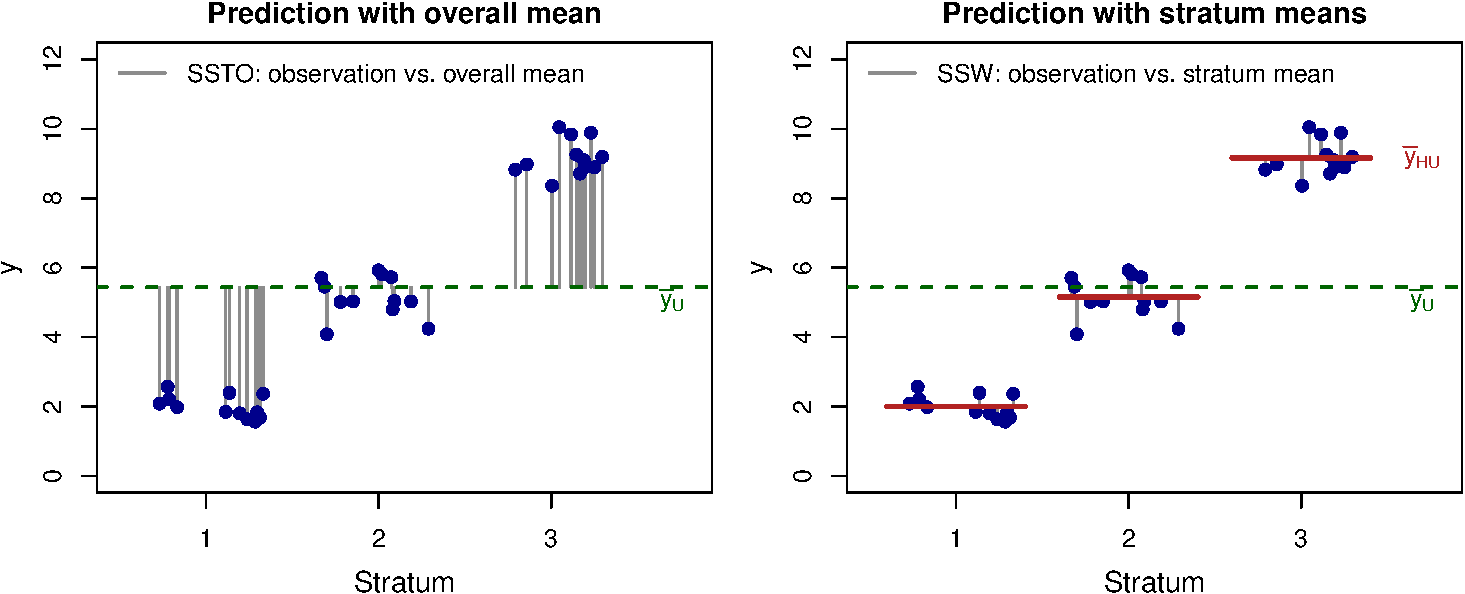
\includegraphics[width=1\linewidth,height=\textheight,keepaspectratio]{strata_files/figure-pdf/fig-ssb-ssw-1.pdf}

}

\caption{\label{fig-ssb-ssw}Left: predicting every unit by the overall
mean (green dashed line); the squared errors (grey) sum to SSTO. Right:
predicting each unit by its stratum mean (red segments); the squared
errors sum to SSW. The difference SSTO − SSW is SSB.}

\end{figure}%

\subsection{\texorpdfstring{The coefficient of determination
\(R^2\)}{The coefficient of determination R\^{}2}}\label{the-coefficient-of-determination-r2}

The share of the total variation that is between strata is the
\textbf{coefficient of determination} \[
R^2 = \frac{\text{SSB}}{\text{SSTO}} = 1-\frac{\text{SSW}}{\text{SSTO}} .
\] \(R^2\) generalizes the squared Pearson correlation coefficient. It
measures how strongly a response \(y\) is related to one or more
predictors. Here the predictor is ``stratum membership'', and \(R^2\) is
the proportion of the variance in \(y\) explained by the strata. It is
the \(R^2\) of a regression of \(y\) on the stratum indicators, as in
the ANOVA fits of Section~\ref{sec-strata-simulation}. When the stratum
means differ widely relative to the spread within each stratum, \(R^2\)
is large (Figure~\ref{fig-r2-compare}, left). When the stratum means are
nearly equal, \(R^2\) is small (right).

\begin{figure}

\centering{

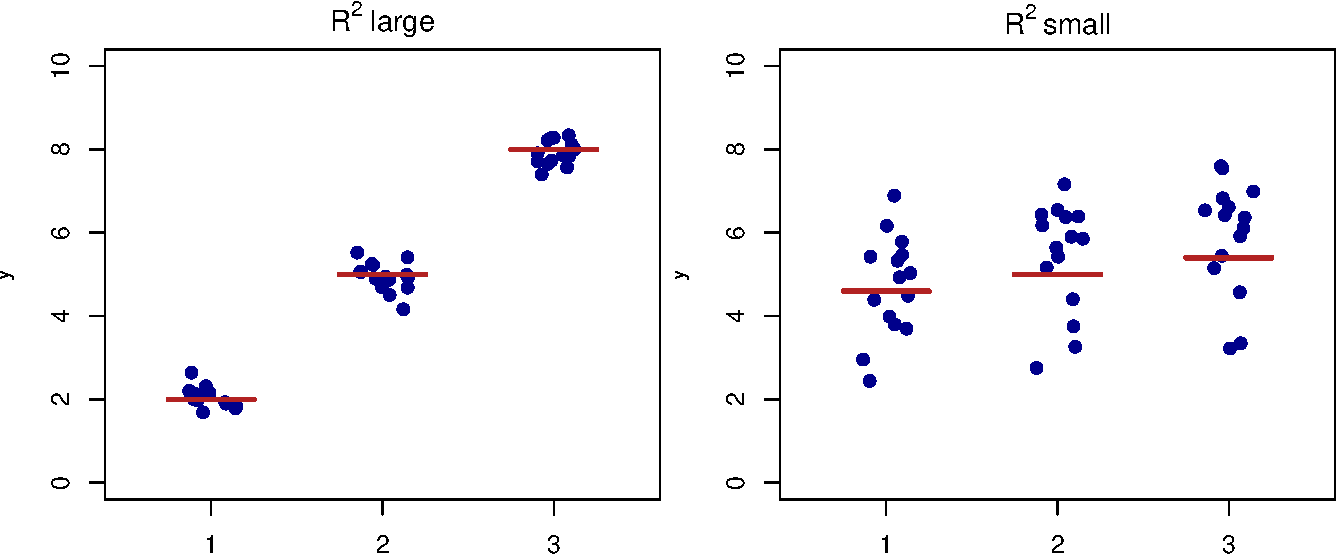
\includegraphics[width=0.9\linewidth,height=\textheight,keepaspectratio]{strata_files/figure-pdf/fig-r2-compare-1.pdf}

}

\caption{\label{fig-r2-compare}Strata with widely separated means (left,
\(R^2\) large) and with nearly equal means (right, \(R^2\) small). Red
segments are the stratum means.}

\end{figure}%

\subsection{Comparing the variances of proportional allocation and
SRS}\label{comparing-the-variances-of-proportional-allocation-and-srs}

Under proportional allocation, \(1 - n_h/N_h = 1-n/N\) and
\(N_h^2/n_h = (N/n)N_h\) for every stratum. So the variance of
\(\hat t_{\text{str}}\) becomes \[
V_{\text{prop}}(\hat t_{\text{str}}) = \Big(1-\frac nN\Big)\frac Nn \sum_{h=1}^H N_h S_h^2
 = \Big(1-\frac nN\Big)\frac Nn\left(\text{SSW} + \sum_{h=1}^H S_h^2\right),
\] using \(\sum_h N_hS_h^2 = \sum_h (N_h-1)S_h^2 + \sum_h S_h^2\).
Equivalently, for the mean, \[
\boxed{V_{\text{prop}}(\overline y_{\text{str}}) = \left(1 - \frac{n}{N}\right)\frac{1}{n}\sum_{h=1}^H \pi_h S_h^2},
\] a weighted average of the within-stratum variances in place of the
overall \(S^2\). For an SRS of the same size \(n\), since
\((N-1)S^2 = \text{SSTO} = \text{SSW}+\text{SSB}\), \[
V_{\text{SRS}}(\hat t) = \Big(1-\frac nN\Big)\frac{N^2 S^2}{n}
 = \Big(1-\frac nN\Big)\frac{N}{n}\cdot\frac{N}{N-1}\,(\text{SSW}+\text{SSB}).
\]

\textbf{When does stratification help?} Comparing the two expressions,
\(V_{\text{prop}} < V_{\text{SRS}}\) exactly when
\((N-1)\big(\text{SSW} + \sum_h S_h^2\big) < N(\text{SSW}+\text{SSB})\).
Substituting \(\text{SSW} = \sum_h(N_h-1)S_h^2\) and simplifying, the
condition becomes \[
\text{SSB} > \sum_{h=1}^H \Big(1-\frac{N_h}{N}\Big)S_h^2 .
\] This almost always holds. SSB is a sum of \(N\) squared deviations,
one for each unit in the population. The right side has only \(H\)
terms, typically far fewer. Proportional allocation can lose to SRS only
when the stratum means are almost identical, and even then the loss is
negligible. In practice stratification with proportional allocation is
never worse than SRS, up to terms of order \(1/N_h\).

\textbf{How much does it help?} Dropping the small terms
\(\sum_h S_h^2\) and \(N/(N-1)\), the ratio of the variances is \[
\frac{V_{\text{prop}}(\hat t_{\text{str}})}{V_{\text{SRS}}(\hat t)}
 \approx \frac{\text{SSW}+\sum_h S_h^2}{\text{SSW}+\text{SSB}} \approx \frac{\text{SSW}}{\text{SSTO}} = 1 - R^2,
\] so that \[
\boxed{\text{percentage of variance reduction} \approx \frac{\text{SSB}}{\text{SSTO}} = R^2_{y\mid\text{strata}}},
\] the proportion of the variance of \(y\) explained by stratum
membership. The better the strata separate the values of \(y\), the
larger the gain. We verify this relation by simulation in
Section~\ref{sec-strata-simulation}.

\section{Optimal Allocation}\label{sec-strata-optimal}

\subsection{The cost function}\label{the-cost-function}

The aim of optimal allocation is to gain the most information for the
least cost. Let \(C\) be the total cost of the survey, \(c_0\) the
overhead cost, and \(c_h\) the cost of sampling one unit in stratum
\(h\): \[
C = c_0 + \sum_{h=1}^H c_h n_h .
\] We want to choose \(n_1,\ldots,n_H\) to minimize
\(V(\overline y_{\text{str}})\) for a fixed total cost \(C\), or,
equivalently, to minimize \(C\) for a fixed variance.

\subsection{Derivation}\label{derivation}

Expanding the fpc, the variance separates into a part that depends on
the \(n_h\) and a part that does not: \[
V(\overline y_{\text{str}}) = \sum_{h=1}^H \Big(1-\frac{n_h}{N_h}\Big)\frac{N_h^2}{N^2}\frac{S_h^2}{n_h}
 = \sum_{h=1}^H \frac{N_h^2S_h^2}{N^2}\cdot\frac1{n_h} \;-\; \underbrace{\sum_{h=1}^H \frac{N_hS_h^2}{N^2}}_{\text{free of } n_h}.
\] We minimize the first sum subject to \(c_0+\sum_h c_hn_h = C\), using
the Lagrangian \[
L(n_1,\ldots,n_H,\lambda) = \sum_{h=1}^H \frac{N_h^2S_h^2}{N^2 n_h} + \lambda\Big(c_0+\sum_{h=1}^H c_hn_h - C\Big).
\] Setting \(\partial L/\partial n_h = 0\) gives \[
-\frac{N_h^2S_h^2}{N^2n_h^2} + \lambda c_h = 0
\quad\Longrightarrow\quad
n_h = \frac{1}{N\sqrt\lambda}\cdot\frac{N_hS_h}{\sqrt{c_h}} .
\] Summing over \(h\) gives
\(n = \frac{1}{N\sqrt\lambda}\sum_{l} N_lS_l/\sqrt{c_l}\). Dividing
\(n_h\) by \(n\) eliminates \(\lambda\).

\subsection{The optimal allocation}\label{the-optimal-allocation}

The optimal \(n_h\) is proportional to \(N_hS_h/\sqrt{c_h}\): \[
\boxed{
n_h = \left(\frac{N_hS_h/\sqrt{c_h}}{\sum_{l=1}^H N_lS_l/\sqrt{c_l}}\right)n,
\qquad n_h \propto \frac{N_hS_h}{\sqrt{c_h}} .}
\] The total \(n\) itself follows from the budget, or from a target
variance. The formula says to sample more heavily in a stratum when:

\begin{itemize}
\tightlist
\item
  the stratum is a large part of the population (\(N_h\) large);
\item
  the stratum is more variable (\(S_h\) large); or
\item
  sampling in the stratum is cheap (\(c_h\) small).
\end{itemize}

Two special cases are important. If the costs are equal,
\(c_1=\cdots=c_H\), then \(n_h\propto N_hS_h\). This is \textbf{Neyman
allocation}: \[
\boxed{n_h = n \frac{N_h S_h}{\sum_{l=1}^H N_l S_l}},
\] which gives the smallest possible variance for a total sample size
\(n\): \[
\boxed{V_{\text{opt}}(\overline{y}_{\text{str}}) = \frac{1}{n}\left(\sum_{h=1}^H \pi_h S_h\right)^2 - \frac{1}{N}\sum_{h=1}^H \pi_h S_h^2}.
\] If, in addition, the stratum standard deviations are equal,
\(S_1=\cdots=S_H\), then \(n_h\propto N_h\), which is proportional
allocation. Neyman allocation improves on proportional allocation
exactly when the \(S_h\) differ across strata.

In practice the \(S_h\) are unknown when the survey is designed. They
are replaced by estimates from a previous survey or a pilot sample, or
by rough guesses. The allocation is fairly robust to such guesses:
moderately wrong values of \(S_h\) still give a variance close to the
optimum.

\subsection{Example: Neyman allocation for the caribou
survey}\label{example-neyman-allocation-for-the-caribou-survey}

To plan the caribou survey of Section~\ref{sec-strata-caribou}, the
investigators used rough estimates of the caribou counts as a proxy for
\(S_h\), with a total sample size of \(n=225\):

{\def\LTcaptype{none} % do not increment counter
\begin{longtable}[]{@{}
  >{\centering\arraybackslash}p{(\linewidth - 10\tabcolsep) * \real{0.1667}}
  >{\raggedleft\arraybackslash}p{(\linewidth - 10\tabcolsep) * \real{0.1000}}
  >{\raggedleft\arraybackslash}p{(\linewidth - 10\tabcolsep) * \real{0.2000}}
  >{\raggedleft\arraybackslash}p{(\linewidth - 10\tabcolsep) * \real{0.2000}}
  >{\raggedleft\arraybackslash}p{(\linewidth - 10\tabcolsep) * \real{0.1667}}
  >{\raggedleft\arraybackslash}p{(\linewidth - 10\tabcolsep) * \real{0.1667}}@{}}
\toprule\noalign{}
\begin{minipage}[b]{\linewidth}\centering
Stratum
\end{minipage} & \begin{minipage}[b]{\linewidth}\raggedleft
\(N_h\)
\end{minipage} & \begin{minipage}[b]{\linewidth}\raggedleft
\(s_h\)
\end{minipage} & \begin{minipage}[b]{\linewidth}\raggedleft
\(N_hs_h\)
\end{minipage} & \begin{minipage}[b]{\linewidth}\raggedleft
\(n_h\) (Neyman)
\end{minipage} & \begin{minipage}[b]{\linewidth}\raggedleft
Sample size used
\end{minipage} \\
\midrule\noalign{}
\endhead
\bottomrule\noalign{}
\endlastfoot
A & 400 & 3,000 & 1,200,000 & 96.26 & 98 \\
B & 30 & 2,000 & 60,000 & 4.81 & 10 \\
C & 61 & 9,000 & 549,000 & 44.04 & 37 \\
D & 18 & 2,000 & 36,000 & 2.89 & 6 \\
E & 70 & 12,000 & 840,000 & 67.38 & 39 \\
F & 120 & 1,000 & 120,000 & 9.63 & 21 \\
\textbf{Total} & \textbf{699} & & \textbf{2,805,000} & \textbf{225} &
\textbf{211} \\
\end{longtable}
}

For example, stratum E gets
\(225 \times 840{,}000/2{,}805{,}000 = 67.38\) units. It has only 10\%
of the population units, but it was expected to be the most variable.
The investigators wanted the sampling fraction to be at least \(1/3\) in
the smaller strata, so they used the Neyman values only as a guideline.
The small strata B, D and F received more units than Neyman allocation
suggests, and stratum E received fewer.

\subsection{Example: Seal holes
(seals.csv)}\label{example-seal-holes-seals.csv}

This dataset comes from a survey of ringed seal breathing holes in three
zones. The researchers used proportional allocation, sampling 20\% of
the areas in each zone.

\begin{Shaded}
\begin{Highlighting}[]
\DocumentationTok{\#\# load data}
\NormalTok{seals }\OtherTok{\textless{}{-}} \FunctionTok{read.csv}\NormalTok{(}\StringTok{"data/seals.csv"}\NormalTok{)}

\CommentTok{\# survey data summary in each stratum}
\NormalTok{nh }\OtherTok{\textless{}{-}} \FunctionTok{as.vector}\NormalTok{(}\FunctionTok{table}\NormalTok{(seals[,}\StringTok{"zone"}\NormalTok{]))}
\NormalTok{sh }\OtherTok{\textless{}{-}} \FunctionTok{tapply}\NormalTok{(seals[, }\StringTok{"holes"}\NormalTok{], seals[,}\StringTok{"zone"}\NormalTok{], sd)}
\NormalTok{ybarh }\OtherTok{\textless{}{-}} \FunctionTok{tapply}\NormalTok{(seals[, }\StringTok{"holes"}\NormalTok{], seals[,}\StringTok{"zone"}\NormalTok{], mean)}
\NormalTok{Nh }\OtherTok{\textless{}{-}} \FunctionTok{c}\NormalTok{(}\DecValTok{68}\NormalTok{, }\DecValTok{84}\NormalTok{, }\DecValTok{48}\NormalTok{)}

\NormalTok{res\_seals }\OtherTok{\textless{}{-}} \FunctionTok{str\_est}\NormalTok{(ybarh, sh, nh, Nh, }\AttributeTok{estimate =} \StringTok{"mean"}\NormalTok{)}
\NormalTok{res\_seals}\SpecialCharTok{$}\NormalTok{table}
\end{Highlighting}
\end{Shaded}

\begin{table}[H]
\caption*{
{\large  Stratified Mean Estimation: Working Table\normalsize }
} 
\normalsize
\begin{gtfit}{\linewidth}{>{\raggedright\arraybackslash}p{\dimexpr 82.50pt -2\tabcolsep-1.5\arrayrulewidth}>{\raggedleft\arraybackslash}p{\dimexpr 45.00pt -2\tabcolsep-1.5\arrayrulewidth}>{\raggedleft\arraybackslash}p{\dimexpr 45.00pt -2\tabcolsep-1.5\arrayrulewidth}>{\raggedleft\arraybackslash}p{\dimexpr 82.50pt -2\tabcolsep-1.5\arrayrulewidth}>{\raggedleft\arraybackslash}p{\dimexpr 82.50pt -2\tabcolsep-1.5\arrayrulewidth}>{\raggedleft\arraybackslash}p{\dimexpr 82.50pt -2\tabcolsep-1.5\arrayrulewidth}>{\raggedleft\arraybackslash}p{\dimexpr 82.50pt -2\tabcolsep-1.5\arrayrulewidth}>{\raggedleft\arraybackslash}p{\dimexpr 82.50pt -2\tabcolsep-1.5\arrayrulewidth}}
\toprule
Stratum & \(N_h\) & \(n_h\) & \(\pi_h\)\textsuperscript{\textit{1}} & \(\bar y_h\) & \(s_h^2\) & \(\pi_h\bar y_h\) & \(v_h\)\textsuperscript{\textit{2}} \\ 
\midrule\addlinespace[2.5pt]
1 & 68 & 17 & 0.34 & 1.76 & 3.32 & 0.60 & 0.02 \\ 
2 & 84 & 12 & 0.42 & 4.42 & 11.54 & 1.85 & 0.15 \\ 
3 & 48 & 11 & 0.24 & 10.55 & 46.07 & 2.53 & 0.19 \\ 
{\bfseries Total} & {\bfseries 200} & {\bfseries 40} & {\bfseries 1.00} & {\bfseries } & {\bfseries } & {\bfseries 4.99} & {\bfseries 0.35} \\ 
\bottomrule
\end{gtfit}
\begin{minipage}{\linewidth}
\vspace{.05em}
\textsuperscript{\textit{1}}\(\pi_h = N_h/N\) is the stratum weight.\\
\textsuperscript{\textit{2}}\(v_h = (1-n_h/N_h)\,\pi_h^2\, s_h^2/n_h\) is stratum \(h\)'s contribution to \(V(\bar y_{str}) = \sum_h v_h\).\\
\(\bar y_{str} = \sum_h \pi_h\bar y_h = 4.99\)\\
\(\mathrm{SE}(\bar y_{str}) = \sqrt{\sum_h v_h} = \sqrt{0.35} = 0.59\)\\
\end{minipage}
\end{table}

Zone 3 has the largest standard deviation (\(s_h \approx 6.8\)), so seal
density varies most there.

\begin{Shaded}
\begin{Highlighting}[]
\NormalTok{res\_seals}\SpecialCharTok{$}\NormalTok{estimate }\SpecialCharTok{|\textgreater{}} \FunctionTok{format\_est\_gt}\NormalTok{(}\StringTok{"mean"}\NormalTok{)}
\end{Highlighting}
\end{Shaded}

\begin{table}[H]
\normalsize
\begin{gtfit}{0.7\linewidth}{rrrr}
\toprule
\(\bar{y}\) & \(\mathrm{SE}(\bar{y})\) & 95\% CI Lower & 95\% CI Upper \\ 
\midrule\addlinespace[2.5pt]
4.99 & 0.59 & 3.83 & 6.14 \\ 
\bottomrule
\end{gtfit}
\end{table}

The estimated mean number of seal holes per area is 5.

Zone 3 was the most variable, so sampling it more heavily would have
lowered the variance. Treating the sample \(s_h\) as estimates of
\(S_h\), and assuming equal costs, we can compute the allocation
proportions \(L_h = n_h/n\) that a future survey should use:

\begin{Shaded}
\begin{Highlighting}[]
\DocumentationTok{\#\# assuming the cost of surveying each zone is the same}
\NormalTok{Ch }\OtherTok{\textless{}{-}} \FunctionTok{rep}\NormalTok{(}\DecValTok{1}\NormalTok{, }\DecValTok{3}\NormalTok{)}
\NormalTok{Sh }\OtherTok{\textless{}{-}}\NormalTok{ sh }\DocumentationTok{\#\# estimate population Sh with sample sh}
\NormalTok{NhShDCh }\OtherTok{\textless{}{-}}\NormalTok{ Nh }\SpecialCharTok{*}\NormalTok{ Sh }\SpecialCharTok{/} \FunctionTok{sqrt}\NormalTok{(Ch)}

\DocumentationTok{\#\# the optimal allocation proportion (Lh) for estimating the population total or mean:}
\NormalTok{Lh }\OtherTok{\textless{}{-}}\NormalTok{ NhShDCh }\SpecialCharTok{/} \FunctionTok{sum}\NormalTok{(NhShDCh)}

\FunctionTok{data.frame}\NormalTok{(Ch, Nh, Sh, NhShDCh, Lh) }\SpecialCharTok{|\textgreater{}}
  \FunctionTok{gt}\NormalTok{(}\AttributeTok{rownames\_to\_stub =} \ConstantTok{TRUE}\NormalTok{) }\SpecialCharTok{|\textgreater{}}
  \FunctionTok{cols\_label}\NormalTok{(}\AttributeTok{NhShDCh =} \FunctionTok{md}\NormalTok{(}\StringTok{"$N\_h S\_h / }\SpecialCharTok{\textbackslash{}\textbackslash{}}\StringTok{sqrt\{C\_h\}$"}\NormalTok{), }\AttributeTok{Lh =} \FunctionTok{md}\NormalTok{(}\StringTok{"$L\_h$ (Prop)"}\NormalTok{), }\AttributeTok{Ch=}\FunctionTok{md}\NormalTok{(}\StringTok{"$C\_h$"}\NormalTok{), }\AttributeTok{Sh=}\FunctionTok{md}\NormalTok{(}\StringTok{"$S\_h$"}\NormalTok{), }\AttributeTok{Nh=}\FunctionTok{md}\NormalTok{(}\StringTok{"$N\_h$"}\NormalTok{)) }\SpecialCharTok{|\textgreater{}}
  \FunctionTok{fmt\_number}\NormalTok{(}\AttributeTok{columns =} \FunctionTok{c}\NormalTok{(Sh, NhShDCh, Lh), }\AttributeTok{decimals =} \DecValTok{3}\NormalTok{)}
\end{Highlighting}
\end{Shaded}

\begin{table}

\caption{\label{tbl-seals-neyman-allocation}Neyman-optimal allocation
proportions for the seals survey zones}

\centering{

\normalsize
\begin{gtfit}{\linewidth}{l|rrrrr}
\toprule
 & \(C_h\) & \(N_h\) & \(S_h\) & \(N_h S_h / \sqrt{C_h}\) & \(L_h\) (Prop) \\ 
\midrule\addlinespace[2.5pt]
1 & 1 & 68 & 1.821 & 123.831 & 0.168 \\ 
2 & 1 & 84 & 3.397 & 285.327 & 0.388 \\ 
3 & 1 & 48 & 6.788 & 325.809 & 0.443 \\ 
\bottomrule
\end{gtfit}

}

\end{table}%

Zone 2 has more areas (\(N_h=84\)), but Zone 3's high variability means
it should receive the largest share of the sampling effort, about 44\%.
Under proportional allocation it received only \(48/200 = 24\%\).

\subsection{Example: Optimal allocation for
polls}\label{example-optimal-allocation-for-polls}

For estimating a proportion, \(S_h^2 \approx p_h(1-p_h)\). As a function
of \(p\), \(p(1-p)\) is a quadratic maximized at \(p=1/2\)
(Figure~\ref{fig-p1mp}). Election regions where support is near 50\%,
the ``swing states'', contribute the most variance per unit sampled.
Optimal allocation therefore gives them relatively larger samples. The
curve is flat near its maximum: \(p(1-p)\) is 0.21 at \(p = 0.3\) and
still 0.25 at \(p = 0.5\). So Neyman allocation for proportions differs
much from proportional allocation only when some \(p_h\) are close to 0
or 1.

\begin{figure}

\centering{

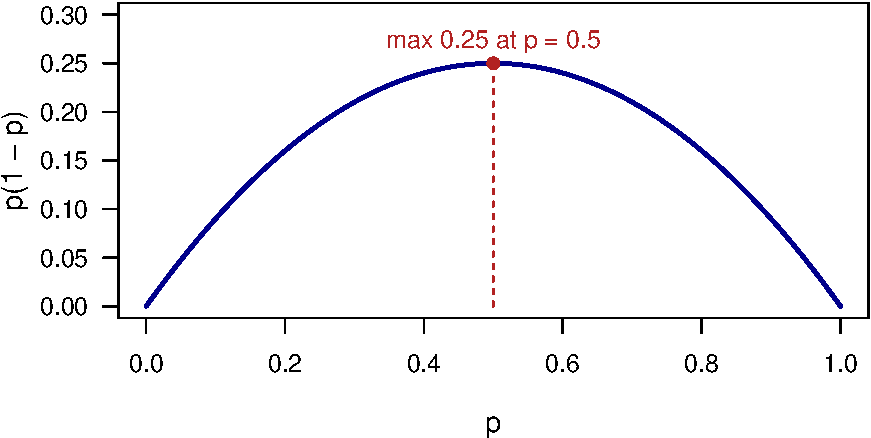
\includegraphics[width=0.6\linewidth,height=\textheight,keepaspectratio]{strata_files/figure-pdf/fig-p1mp-1.pdf}

}

\caption{\label{fig-p1mp}The variance of a 0/1 variable, \(p(1-p)\), is
largest at \(p = 0.5\).}

\end{figure}%

\subsection{Example: Dollar
stratification}\label{example-dollar-stratification}

\textbf{Dollar stratification} is common in accounting audits. The
recorded book amounts are used to stratify the population. For example,
stratum 1 might be all loans over \$1 million, stratum 2 the loans
between \$500,000 and \$999,999, and so on, down to loans under
\$10,000. Optimal allocation is very efficient here. \(S_h\) is much
larger in the strata with large loan amounts, so optimal allocation
gives those strata a much higher sampling fraction. Often the top
stratum is sampled completely (\(n_h = N_h\)). This makes sense: an
error in a \$3,000,000 loan is likely to contribute far more to the
total audited discrepancy than an error in a \$3,000 loan.

\section{Choosing Stratification Variables}\label{sec-strata-choice}

Stratification is most efficient when the stratum means differ widely.
Then SSB is large and the variability within the strata is small.
Ideally we would stratify by the values of \(y\) itself. But \(y\) is
unknown before sampling, so we look instead for an \textbf{auxiliary
variable} \(x\) that is known for every unit in the population and is
highly correlated with \(y\). Cutting the range of \(x\) into intervals
then produces strata whose distributions of \(y\) differ
(Figure~\ref{fig-auxiliary}).

\begin{figure}

\centering{

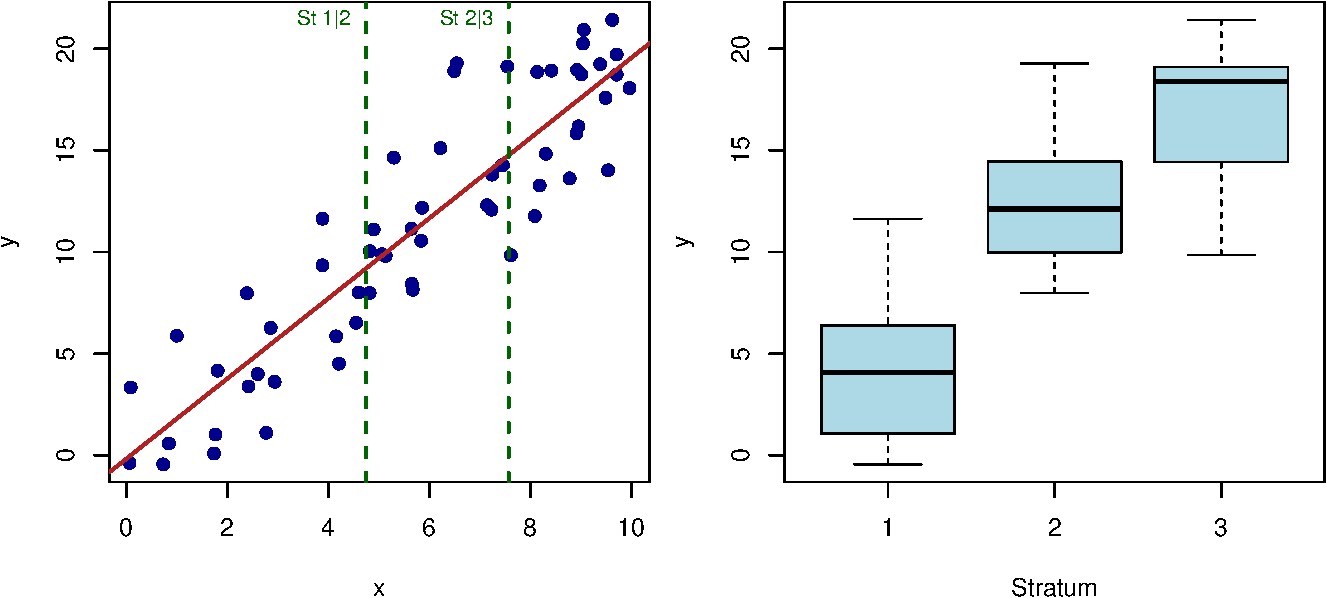
\includegraphics[width=0.9\linewidth,height=\textheight,keepaspectratio]{strata_files/figure-pdf/fig-auxiliary-1.pdf}

}

\caption{\label{fig-auxiliary}Cutting an auxiliary variable \(x\) at its
terciles (left, dashed lines) produces strata with visibly different
distributions of \(y\) (right).}

\end{figure}%

Some examples:

\begin{itemize}
\tightlist
\item
  To estimate total business expenditure on advertising, we would like
  the businesses that spend the most on advertising in stratum 1, the
  next highest spenders in stratum 2, and so on. We might stratify by
  the number of employees or the size of the business, and by the type
  of product or service.
\item
  For farm income, we might use farm size as the stratification
  variable, since we expect larger farms to have higher incomes.
\item
  For the county farm data, the acreage in an earlier census
  (\texttt{acres82}) is known for every county and is much more strongly
  related to \texttt{acres92} than the region is.
  Section~\ref{sec-strata-simulation} shows how much this matters.
\end{itemize}

Stratified sampling also has limitations:

\begin{itemize}
\tightlist
\item
  \textbf{It requires information before sampling.} We need the stratum
  membership of every unit and the stratum sizes \(N_h\). For optimal
  allocation we also need rough values of \(S_h\).
\item
  \textbf{One survey usually measures many variables.} A stratification
  variable that works well for one \(y\) may work poorly for another. A
  variable highly correlated with one outcome may be nearly uncorrelated
  with another outcome measured in the same survey. Proportional
  allocation is a safe compromise, since it never does materially worse
  than SRS for any variable. An allocation that is optimal for one
  variable can be inefficient for others.
\end{itemize}

\section{Simulation: Efficiency of Stratification and
Allocation}\label{sec-strata-simulation}

We now check the theory by simulation. The full \texttt{agpop.csv}
dataset serves as the population. We draw 2000 repeated samples of
\(n = 300\) counties under three designs, SRS, proportional allocation
(P2S) and Neyman allocation, and compare the spread of the resulting
estimates of \(\overline y_U\). We do this twice, with two different
stratification variables.

\subsection{Stratifying by region}\label{stratifying-by-region}

\begin{Shaded}
\begin{Highlighting}[]
\NormalTok{agpop }\OtherTok{\textless{}{-}} \FunctionTok{acres\_in\_thousands}\NormalTok{(}\FunctionTok{read.csv}\NormalTok{(}\StringTok{"data/agpop.csv"}\NormalTok{))}
\NormalTok{agpop }\OtherTok{\textless{}{-}}\NormalTok{ agpop[}\SpecialCharTok{!}\FunctionTok{is.na}\NormalTok{(agpop}\SpecialCharTok{$}\NormalTok{acres92), ] }\DocumentationTok{\#\# remove those counties with na}
\NormalTok{N }\OtherTok{\textless{}{-}} \FunctionTok{nrow}\NormalTok{(agpop)}
\end{Highlighting}
\end{Shaded}

\begin{Shaded}
\begin{Highlighting}[]
\NormalTok{agpop}\SpecialCharTok{$}\NormalTok{stratum }\OtherTok{\textless{}{-}}\NormalTok{ agpop}\SpecialCharTok{$}\NormalTok{region}
\DocumentationTok{\#\# reorder agpop for the ease of using strata of "sampling" (very important)}
\NormalTok{agpop }\OtherTok{\textless{}{-}}\NormalTok{ agpop[}\FunctionTok{order}\NormalTok{(agpop}\SpecialCharTok{$}\NormalTok{stratum), ]}
\end{Highlighting}
\end{Shaded}

Section~\ref{sec-strata-prop} showed that the variance reduction under
proportional allocation is about \(R^2\), the proportion of the variance
of \(y\) explained by the strata. We compute it with a one-way ANOVA of
\texttt{acres92} on the strata.

\begin{Shaded}
\begin{Highlighting}[]
\FunctionTok{boxplot}\NormalTok{(acres92 }\SpecialCharTok{\textasciitilde{}}\NormalTok{ stratum, }\AttributeTok{data =}\NormalTok{ agpop)}
\end{Highlighting}
\end{Shaded}

\begin{figure}[H]

\centering{

\pandocbounded{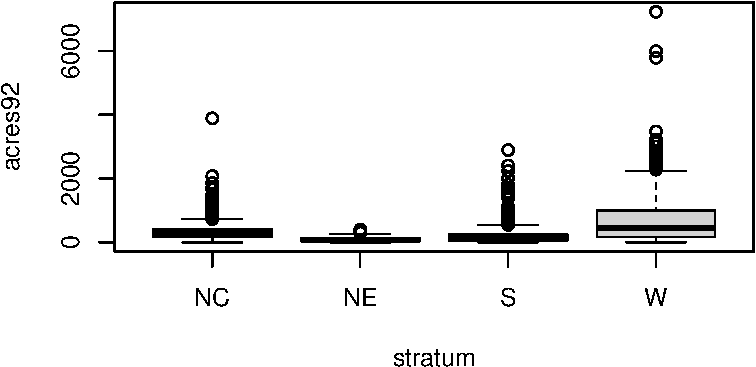
\includegraphics[keepaspectratio]{strata_files/figure-pdf/fig-agpop-region-boxplot-1.pdf}}

}

\caption{\label{fig-agpop-region-boxplot}1992 farm acreage by region
stratum}

\end{figure}%

\begin{Shaded}
\begin{Highlighting}[]
\NormalTok{lm\_region }\OtherTok{\textless{}{-}} \FunctionTok{lm}\NormalTok{(agpop}\SpecialCharTok{$}\NormalTok{acres92 }\SpecialCharTok{\textasciitilde{}}\NormalTok{ agpop}\SpecialCharTok{$}\NormalTok{stratum)}
\FunctionTok{anova}\NormalTok{(lm\_region)}
\end{Highlighting}
\end{Shaded}

\begin{verbatim}
Analysis of Variance Table

Response: agpop$acres92
                Df    Sum Sq  Mean Sq F value    Pr(>F)    
agpop$stratum    3 100733006 33577669  226.73 < 2.2e-16 ***
Residuals     3055 452431724   148095                      
---
Signif. codes:  0 '***' 0.001 '**' 0.01 '*' 0.05 '.' 0.1 ' ' 1
\end{verbatim}

\begin{Shaded}
\begin{Highlighting}[]
\NormalTok{lm\_region\_gt }\OtherTok{\textless{}{-}} \FunctionTok{format\_lm\_gt}\NormalTok{(lm\_region)}
\NormalTok{lm\_region\_gt}\SpecialCharTok{$}\NormalTok{fit}
\end{Highlighting}
\end{Shaded}

\begin{table}[H]
\caption*{
{\large  Model Fit Summary\normalsize }
} 
\normalsize
\begin{gtfit}{0.7\linewidth}{rrrrr}
\toprule
\(R^2\) & Adj. \(R^2\) & \(\hat\sigma\) & F-statistic & p-value \\ 
\midrule\addlinespace[2.5pt]
0.1821 & 0.1813 & 384.8318 & 226.7299 & 0.0000 \\ 
\bottomrule
\end{gtfit}
\end{table}

\begin{Shaded}
\begin{Highlighting}[]
\NormalTok{r\_squared\_region }\OtherTok{\textless{}{-}} \FunctionTok{summary}\NormalTok{(lm\_region)}\SpecialCharTok{$}\NormalTok{r.squared}
\end{Highlighting}
\end{Shaded}

The R-squared is 0.182. Region explains only about 18.2\% of the
variance in acreage. That is helpful, but not strong.

\subsubsection*{A single stratified sample with proportional
allocation}\label{a-single-stratified-sample-with-proportional-allocation}
\addcontentsline{toc}{subsubsection}{A single stratified sample with
proportional allocation}

The function \texttt{strata()} from the \textbf{sampling} package draws
an SRS of the given size in each stratum. The data must be sorted by
stratum. The sampling weights are the reciprocals of the inclusion
probabilities it returns.

\begin{Shaded}
\begin{Highlighting}[]
\CommentTok{\# doing one stratified sampling}
\NormalTok{Nh }\OtherTok{\textless{}{-}} \FunctionTok{tapply}\NormalTok{(}\DecValTok{1}\SpecialCharTok{:}\FunctionTok{nrow}\NormalTok{(agpop), agpop}\SpecialCharTok{$}\NormalTok{stratum, length)}
\NormalTok{nh }\OtherTok{\textless{}{-}} \FunctionTok{round}\NormalTok{(Nh}\SpecialCharTok{/}\FunctionTok{sum}\NormalTok{(Nh)}\SpecialCharTok{*}\DecValTok{300}\NormalTok{)}

\DocumentationTok{\#\# doing stratified sampling}
\NormalTok{strsample }\OtherTok{\textless{}{-}} \FunctionTok{strata}\NormalTok{(agpop, }\StringTok{"stratum"}\NormalTok{, }\AttributeTok{size =}\NormalTok{ nh, }\AttributeTok{method =} \StringTok{"srswor"}\NormalTok{)}

\CommentTok{\# collecting data on sampled counties}
\NormalTok{agstrat }\OtherTok{\textless{}{-}}\NormalTok{ agpop[strsample}\SpecialCharTok{$}\NormalTok{ID\_unit, ]}
\NormalTok{agstrat}\SpecialCharTok{$}\NormalTok{weight }\OtherTok{\textless{}{-}} \DecValTok{1}\SpecialCharTok{/}\NormalTok{strsample}\SpecialCharTok{$}\NormalTok{Prob}

\FunctionTok{str\_est\_data}\NormalTok{(agstrat, }\StringTok{"acres92"}\NormalTok{, }\StringTok{"stratum"}\NormalTok{, }\StringTok{"weight"}\NormalTok{, }\AttributeTok{estimate =} \StringTok{"mean"}\NormalTok{)}\SpecialCharTok{$}\NormalTok{estimate }\SpecialCharTok{|\textgreater{}}
  \FunctionTok{format\_est\_gt}\NormalTok{(}\StringTok{"mean"}\NormalTok{)}
\end{Highlighting}
\end{Shaded}

\begin{table}[H]
\normalsize
\begin{gtfit}{0.7\linewidth}{rrrr}
\toprule
\(\bar{y}\) & \(\mathrm{SE}(\bar{y})\) & 95\% CI Lower & 95\% CI Upper \\ 
\midrule\addlinespace[2.5pt]
328.10 & 18.65 & 291.55 & 364.65 \\ 
\bottomrule
\end{gtfit}
\end{table}

\subsubsection*{Repeating proportional allocation 2000
times}\label{repeating-proportional-allocation-2000-times}
\addcontentsline{toc}{subsubsection}{Repeating proportional allocation
2000 times}

\begin{Shaded}
\begin{Highlighting}[]
\NormalTok{Nh }\OtherTok{\textless{}{-}} \FunctionTok{tapply}\NormalTok{(}\DecValTok{1}\SpecialCharTok{:}\FunctionTok{nrow}\NormalTok{(agpop), agpop}\SpecialCharTok{$}\NormalTok{stratum, length)}
\NormalTok{nh }\OtherTok{\textless{}{-}} \FunctionTok{round}\NormalTok{(Nh}\SpecialCharTok{/}\FunctionTok{sum}\NormalTok{(Nh)}\SpecialCharTok{*}\DecValTok{300}\NormalTok{) }\DocumentationTok{\#\# make sure the order matches Nh}

\NormalTok{nres }\OtherTok{\textless{}{-}} \DecValTok{2000}
\NormalTok{str\_p2s\_simulated }\OtherTok{\textless{}{-}} \FunctionTok{matrix}\NormalTok{(}\DecValTok{0}\NormalTok{, nres, }\DecValTok{4}\NormalTok{)}
\ControlFlowTok{for}\NormalTok{ (i }\ControlFlowTok{in} \DecValTok{1}\SpecialCharTok{:}\NormalTok{nres) \{}
\NormalTok{    strsample }\OtherTok{\textless{}{-}} \FunctionTok{strata}\NormalTok{(agpop, }\StringTok{"stratum"}\NormalTok{, }\AttributeTok{size =}\NormalTok{ nh, }\AttributeTok{method =} \StringTok{"srswor"}\NormalTok{)}
\NormalTok{    agstrat }\OtherTok{\textless{}{-}}\NormalTok{ agpop[strsample}\SpecialCharTok{$}\NormalTok{ID\_unit, ]}
\NormalTok{    agstrat}\SpecialCharTok{$}\NormalTok{weight }\OtherTok{\textless{}{-}} \DecValTok{1}\SpecialCharTok{/}\NormalTok{strsample}\SpecialCharTok{$}\NormalTok{Prob}
\NormalTok{    str\_p2s\_simulated[i,] }\OtherTok{\textless{}{-}} \FunctionTok{str\_est\_data}\NormalTok{(agstrat, }\StringTok{"acres92"}\NormalTok{, }\StringTok{"stratum"}\NormalTok{, }\StringTok{"weight"}\NormalTok{, }\AttributeTok{estimate =} \StringTok{"mean"}\NormalTok{, }\AttributeTok{show.details =} \ConstantTok{FALSE}\NormalTok{)}\SpecialCharTok{$}\NormalTok{estimate}
\NormalTok{\}}
\end{Highlighting}
\end{Shaded}

\subsubsection*{Repeating Neyman allocation 2000
times}\label{repeating-neyman-allocation-2000-times}
\addcontentsline{toc}{subsubsection}{Repeating Neyman allocation 2000
times}

In a simulation the population \(S_h\) are known, so we can use the
exact Neyman allocation:

\begin{Shaded}
\begin{Highlighting}[]
\NormalTok{Nh }\OtherTok{\textless{}{-}} \FunctionTok{tapply}\NormalTok{(agpop}\SpecialCharTok{$}\NormalTok{acres92, agpop}\SpecialCharTok{$}\NormalTok{stratum, length)}
\NormalTok{Sh }\OtherTok{\textless{}{-}} \FunctionTok{tapply}\NormalTok{(agpop}\SpecialCharTok{$}\NormalTok{acres92, agpop}\SpecialCharTok{$}\NormalTok{stratum, sd)}
\NormalTok{nh\_opt }\OtherTok{\textless{}{-}} \FunctionTok{round}\NormalTok{((Nh}\SpecialCharTok{*}\NormalTok{Sh)}\SpecialCharTok{/}\FunctionTok{sum}\NormalTok{(Nh}\SpecialCharTok{*}\NormalTok{Sh) }\SpecialCharTok{*} \DecValTok{300}\NormalTok{)}

\FunctionTok{data.frame}\NormalTok{(Nh, Sh, nh\_opt) }\SpecialCharTok{|\textgreater{}}
  \FunctionTok{gt}\NormalTok{(}\AttributeTok{rownames\_to\_stub =} \ConstantTok{TRUE}\NormalTok{) }\SpecialCharTok{|\textgreater{}}
  \FunctionTok{fmt\_number}\NormalTok{(}\AttributeTok{columns =}\NormalTok{ Sh, }\AttributeTok{decimals =} \DecValTok{2}\NormalTok{)}
\end{Highlighting}
\end{Shaded}

\begin{table}

\caption{\label{tbl-agpop-region-neyman-allocation}Population sizes and
Neyman-optimal sample sizes by region stratum}

\centering{

\normalsize
\begin{gtfit}{\linewidth}{l|rrr}
\toprule
 & Nh & Sh & nh\_opt \\ 
\midrule\addlinespace[2.5pt]
NC & 1052 & 271.19 & 87 \\ 
NE & 213 & 78.91 & 5 \\ 
S & 1376 & 244.13 & 102 \\ 
W & 418 & 836.61 & 106 \\ 
\bottomrule
\end{gtfit}

}

\end{table}%

The West, with the largest \(S_h\), receives a disproportionately large
sample under Neyman allocation.

\begin{Shaded}
\begin{Highlighting}[]
\NormalTok{nres }\OtherTok{\textless{}{-}} \DecValTok{2000}
\NormalTok{str\_neyman\_simulated }\OtherTok{\textless{}{-}} \FunctionTok{matrix}\NormalTok{(}\DecValTok{0}\NormalTok{, nres, }\DecValTok{4}\NormalTok{)}
\ControlFlowTok{for}\NormalTok{ (i }\ControlFlowTok{in} \DecValTok{1}\SpecialCharTok{:}\NormalTok{nres) \{}
\NormalTok{    strsample }\OtherTok{\textless{}{-}} \FunctionTok{strata}\NormalTok{(agpop, }\StringTok{"stratum"}\NormalTok{, }\AttributeTok{size =}\NormalTok{ nh\_opt, }\AttributeTok{method =} \StringTok{"srswor"}\NormalTok{)}
\NormalTok{    agstrat }\OtherTok{\textless{}{-}}\NormalTok{ agpop[strsample}\SpecialCharTok{$}\NormalTok{ID\_unit, ]}
\NormalTok{    agstrat}\SpecialCharTok{$}\NormalTok{weight }\OtherTok{\textless{}{-}} \DecValTok{1}\SpecialCharTok{/}\NormalTok{strsample}\SpecialCharTok{$}\NormalTok{Prob}
\NormalTok{    str\_neyman\_simulated[i,] }\OtherTok{\textless{}{-}} \FunctionTok{str\_est\_data}\NormalTok{(agstrat, }\StringTok{"acres92"}\NormalTok{, }\StringTok{"stratum"}\NormalTok{, }\StringTok{"weight"}\NormalTok{, }\AttributeTok{estimate =} \StringTok{"mean"}\NormalTok{, }\AttributeTok{show.details =} \ConstantTok{FALSE}\NormalTok{)}\SpecialCharTok{$}\NormalTok{estimate}
\NormalTok{\}}
\end{Highlighting}
\end{Shaded}

\subsubsection*{Repeating SRS 2000
times}\label{repeating-srs-2000-times}
\addcontentsline{toc}{subsubsection}{Repeating SRS 2000 times}

\begin{Shaded}
\begin{Highlighting}[]
\NormalTok{nres }\OtherTok{\textless{}{-}} \DecValTok{2000}
\NormalTok{srs\_simulated }\OtherTok{\textless{}{-}} \FunctionTok{matrix}\NormalTok{(}\DecValTok{0}\NormalTok{, nres, }\DecValTok{4}\NormalTok{)}
\ControlFlowTok{for}\NormalTok{ (i }\ControlFlowTok{in} \DecValTok{1}\SpecialCharTok{:}\NormalTok{nres) \{}
\NormalTok{    srs }\OtherTok{\textless{}{-}} \FunctionTok{sample}\NormalTok{(}\FunctionTok{sum}\NormalTok{(Nh), }\FunctionTok{sum}\NormalTok{(nh))}
\NormalTok{    agsrs }\OtherTok{\textless{}{-}}\NormalTok{ agpop[srs, ]}
\NormalTok{    srs\_simulated[i,] }\OtherTok{\textless{}{-}} \FunctionTok{srs\_est}\NormalTok{(agsrs[, }\StringTok{"acres92"}\NormalTok{], }\AttributeTok{N =} \FunctionTok{sum}\NormalTok{(Nh), }\AttributeTok{estimate =} \StringTok{"mean"}\NormalTok{, }\AttributeTok{show.details =} \ConstantTok{FALSE}\NormalTok{)}\SpecialCharTok{$}\NormalTok{estimate}
\NormalTok{\}}
\end{Highlighting}
\end{Shaded}

\subsubsection*{Comparing the three
designs}\label{comparing-the-three-designs}
\addcontentsline{toc}{subsubsection}{Comparing the three designs}

\begin{Shaded}
\begin{Highlighting}[]
\NormalTok{sim\_results\_str\_region }\OtherTok{\textless{}{-}} \FunctionTok{data.frame}\NormalTok{(}
  \StringTok{"SRS"} \OtherTok{=}\NormalTok{ srs\_simulated[,}\DecValTok{1}\NormalTok{],}
  \StringTok{"Prop2size"} \OtherTok{=}\NormalTok{ str\_p2s\_simulated[,}\DecValTok{1}\NormalTok{],}
  \StringTok{"Neyman"} \OtherTok{=}\NormalTok{ str\_neyman\_simulated[,}\DecValTok{1}\NormalTok{]}
\NormalTok{)}
\FunctionTok{boxplot}\NormalTok{(sim\_results\_str\_region)}
\FunctionTok{abline}\NormalTok{(}\AttributeTok{h =} \FunctionTok{mean}\NormalTok{(agpop}\SpecialCharTok{$}\NormalTok{acres92), }\AttributeTok{col =} \StringTok{"red"}\NormalTok{)}
\end{Highlighting}
\end{Shaded}

\begin{figure}[H]

\centering{

\pandocbounded{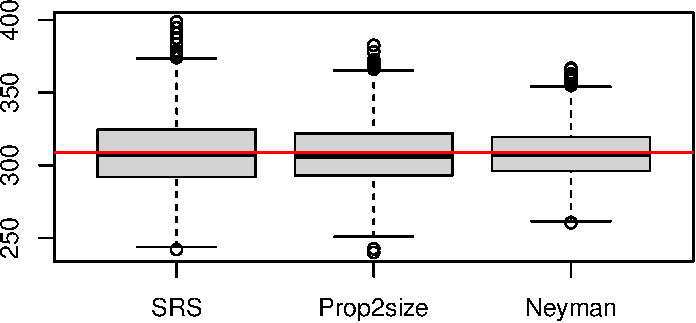
\includegraphics[keepaspectratio]{strata_files/figure-pdf/fig-agpop-region-compare-boxplot-1.pdf}}

}

\caption{\label{fig-agpop-region-compare-boxplot}Sampling distribution
of the mean under SRS, proportional, and Neyman allocation (region
strata, 2000 simulations)}

\end{figure}%

\begin{Shaded}
\begin{Highlighting}[]
\NormalTok{sim\_means }\OtherTok{\textless{}{-}} \FunctionTok{sapply}\NormalTok{(sim\_results\_str\_region, mean)}
\NormalTok{sim\_var }\OtherTok{\textless{}{-}} \FunctionTok{sapply}\NormalTok{(sim\_results\_str\_region, var)}
\NormalTok{sim\_var\_relative }\OtherTok{\textless{}{-}}\NormalTok{ sim\_var }\SpecialCharTok{/}\NormalTok{ sim\_var[}\DecValTok{1}\NormalTok{]}
\NormalTok{sim\_var\_reduction }\OtherTok{\textless{}{-}} \DecValTok{1} \SpecialCharTok{{-}}\NormalTok{ sim\_var\_relative}

\FunctionTok{data.frame}\NormalTok{(}
  \StringTok{"Mean"} \OtherTok{=}\NormalTok{ sim\_means,}
  \StringTok{"Variance"} \OtherTok{=}\NormalTok{ sim\_var,}
  \StringTok{"Relative Variance"} \OtherTok{=}\NormalTok{ sim\_var\_relative,}
  \StringTok{"Percentage of Variance Reduction"} \OtherTok{=}\NormalTok{ sim\_var\_reduction,}
  \AttributeTok{check.names =} \ConstantTok{FALSE}
\NormalTok{) }\SpecialCharTok{|\textgreater{}}
  \FunctionTok{gt}\NormalTok{(}\AttributeTok{rownames\_to\_stub =} \ConstantTok{TRUE}\NormalTok{) }\SpecialCharTok{|\textgreater{}}
  \FunctionTok{fmt\_number}\NormalTok{(}\AttributeTok{columns =} \FunctionTok{c}\NormalTok{(Mean, Variance), }\AttributeTok{decimals =} \DecValTok{1}\NormalTok{) }\SpecialCharTok{|\textgreater{}}
  \FunctionTok{fmt\_percent}\NormalTok{(}\AttributeTok{columns =} \FunctionTok{c}\NormalTok{(}\StringTok{\textasciigrave{}}\AttributeTok{Percentage of Variance Reduction}\StringTok{\textasciigrave{}}\NormalTok{), }\AttributeTok{decimals =} \DecValTok{2}\NormalTok{) }\SpecialCharTok{|\textgreater{}}
  \FunctionTok{fmt\_number}\NormalTok{(}\AttributeTok{columns =} \FunctionTok{c}\NormalTok{(}\StringTok{\textasciigrave{}}\AttributeTok{Relative Variance}\StringTok{\textasciigrave{}}\NormalTok{), }\AttributeTok{decimals =} \DecValTok{3}\NormalTok{)}
\end{Highlighting}
\end{Shaded}

\begin{table}

\caption{\label{tbl-agpop-region-compare-methods}Simulated mean,
variance, and variance reduction by allocation method (region strata)}

\centering{

\normalsize
\begin{gtfit}{\linewidth}{l|rrrr}
\toprule
 & Mean & Variance & Relative Variance & Percentage of Variance Reduction \\ 
\midrule\addlinespace[2.5pt]
SRS & 308.9 & 583.4 & 1.000 & 0.00\% \\ 
Prop2size & 307.9 & 452.0 & 0.775 & 22.53\% \\ 
Neyman & 307.9 & 297.0 & 0.509 & 49.09\% \\ 
\bottomrule
\end{gtfit}

}

\end{table}%

All three designs are centred on the true mean (the red line).
Proportional allocation reduces the variance by 22.5\% compared with
SRS, close to \(R^2 = 0.182\) as the theory predicts. Neyman allocation
reduces it by 49.1\%, because the regions differ greatly in their
standard deviations \(S_h\).

\subsection{Stratifying by acres82}\label{stratifying-by-acres82}

Now we stratify by a variable that is highly correlated with the target:
the farm acreage of each county a decade earlier (\texttt{acres82}).

\begin{Shaded}
\begin{Highlighting}[]
\NormalTok{agpop }\OtherTok{\textless{}{-}} \FunctionTok{acres\_in\_thousands}\NormalTok{(}\FunctionTok{read.csv}\NormalTok{(}\StringTok{"data/agpop.csv"}\NormalTok{))}
\DocumentationTok{\#\# acres82 is the stratifier here, so drop the counties missing either variable}
\NormalTok{agpop }\OtherTok{\textless{}{-}}\NormalTok{ agpop[}\SpecialCharTok{!}\FunctionTok{is.na}\NormalTok{(agpop}\SpecialCharTok{$}\NormalTok{acres92) }\SpecialCharTok{\&} \SpecialCharTok{!}\FunctionTok{is.na}\NormalTok{(agpop}\SpecialCharTok{$}\NormalTok{acres82), ]}
\NormalTok{N }\OtherTok{\textless{}{-}} \FunctionTok{nrow}\NormalTok{(agpop)}
\end{Highlighting}
\end{Shaded}

We convert the continuous \texttt{acres82} into four strata by cutting
it at its 25th, 75th and 95th percentiles. The cut is deliberately
uneven. The top 5\% of counties, where the acreages run away, get a
stratum of their own, as in dollar stratification. This is what makes
the stratification so effective below.

\begin{Shaded}
\begin{Highlighting}[]
\NormalTok{agpop}\SpecialCharTok{$}\NormalTok{stratum }\OtherTok{\textless{}{-}} \FunctionTok{cut}\NormalTok{(agpop}\SpecialCharTok{$}\NormalTok{acres82,}
                     \AttributeTok{breaks =} \FunctionTok{quantile}\NormalTok{(agpop}\SpecialCharTok{$}\NormalTok{acres82, }\AttributeTok{probs =} \FunctionTok{c}\NormalTok{(}\DecValTok{0}\NormalTok{,}\FloatTok{0.25}\NormalTok{,}\FloatTok{0.75}\NormalTok{,}\FloatTok{0.95}\NormalTok{,}\DecValTok{1}\NormalTok{)),}
                     \AttributeTok{include.lowest =}\NormalTok{ T)}
\FunctionTok{levels}\NormalTok{(agpop}\SpecialCharTok{$}\NormalTok{stratum) }\OtherTok{\textless{}{-}} \FunctionTok{paste0}\NormalTok{(}\StringTok{"acres82"}\NormalTok{, }\FunctionTok{c}\NormalTok{(}\StringTok{"Q1"}\NormalTok{, }\StringTok{"Q2"}\NormalTok{, }\StringTok{"Q3"}\NormalTok{, }\StringTok{"Q4"}\NormalTok{))}
\NormalTok{agpop }\OtherTok{\textless{}{-}}\NormalTok{ agpop[}\FunctionTok{order}\NormalTok{(agpop}\SpecialCharTok{$}\NormalTok{stratum), ]}
\end{Highlighting}
\end{Shaded}

\begin{Shaded}
\begin{Highlighting}[]
\FunctionTok{boxplot}\NormalTok{(acres92 }\SpecialCharTok{\textasciitilde{}}\NormalTok{ stratum, }\AttributeTok{data =}\NormalTok{ agpop)}
\end{Highlighting}
\end{Shaded}

\begin{figure}[H]

\centering{

\pandocbounded{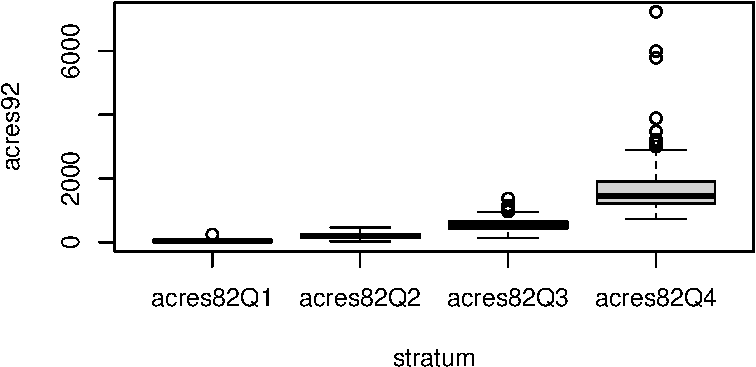
\includegraphics[keepaspectratio]{strata_files/figure-pdf/fig-agpop-acres82-boxplot-1.pdf}}

}

\caption{\label{fig-agpop-acres82-boxplot}1992 farm acreage by acres82
quantile stratum}

\end{figure}%

\begin{Shaded}
\begin{Highlighting}[]
\NormalTok{lm\_acres82 }\OtherTok{\textless{}{-}} \FunctionTok{lm}\NormalTok{(agpop}\SpecialCharTok{$}\NormalTok{acres92 }\SpecialCharTok{\textasciitilde{}}\NormalTok{ agpop}\SpecialCharTok{$}\NormalTok{stratum)}
\NormalTok{lm\_acres82\_gt }\OtherTok{\textless{}{-}} \FunctionTok{format\_lm\_gt}\NormalTok{(lm\_acres82)}
\NormalTok{lm\_acres82\_gt}\SpecialCharTok{$}\NormalTok{fit}
\end{Highlighting}
\end{Shaded}

\begin{table}[H]
\caption*{
{\large  Model Fit Summary\normalsize }
} 
\normalsize
\begin{gtfit}{0.7\linewidth}{rrrrr}
\toprule
\(R^2\) & Adj. \(R^2\) & \(\hat\sigma\) & F-statistic & p-value \\ 
\midrule\addlinespace[2.5pt]
0.7402 & 0.7400 & 216.9580 & 2,895.9129 & 0.0000 \\ 
\bottomrule
\end{gtfit}
\end{table}

\begin{Shaded}
\begin{Highlighting}[]
\NormalTok{r\_squared\_acres82 }\OtherTok{\textless{}{-}} \FunctionTok{summary}\NormalTok{(lm\_acres82)}\SpecialCharTok{$}\NormalTok{r.squared}
\end{Highlighting}
\end{Shaded}

The R-squared is now 0.74: the earlier acreage explains 74\% of the
variance in 1992 acreage. This makes it a far better stratification
variable than region.

\subsubsection*{Repeating proportional allocation 2000
times}\label{repeating-proportional-allocation-2000-times-1}
\addcontentsline{toc}{subsubsection}{Repeating proportional allocation
2000 times}

\begin{Shaded}
\begin{Highlighting}[]
\NormalTok{Nh }\OtherTok{\textless{}{-}} \FunctionTok{tapply}\NormalTok{(}\DecValTok{1}\SpecialCharTok{:}\FunctionTok{nrow}\NormalTok{(agpop), agpop}\SpecialCharTok{$}\NormalTok{stratum, length)}
\NormalTok{nh }\OtherTok{\textless{}{-}} \FunctionTok{round}\NormalTok{(Nh}\SpecialCharTok{/}\FunctionTok{sum}\NormalTok{(Nh)}\SpecialCharTok{*}\DecValTok{300}\NormalTok{)}

\NormalTok{nres }\OtherTok{\textless{}{-}} \DecValTok{2000}
\NormalTok{str\_p2s\_simulated }\OtherTok{\textless{}{-}} \FunctionTok{matrix}\NormalTok{(}\DecValTok{0}\NormalTok{, nres, }\DecValTok{4}\NormalTok{)}
\ControlFlowTok{for}\NormalTok{ (i }\ControlFlowTok{in} \DecValTok{1}\SpecialCharTok{:}\NormalTok{nres) \{}
\NormalTok{    strsample }\OtherTok{\textless{}{-}} \FunctionTok{strata}\NormalTok{(agpop, }\StringTok{"stratum"}\NormalTok{, }\AttributeTok{size =}\NormalTok{ nh, }\AttributeTok{method =} \StringTok{"srswor"}\NormalTok{)}
\NormalTok{    agstrat }\OtherTok{\textless{}{-}}\NormalTok{ agpop[strsample}\SpecialCharTok{$}\NormalTok{ID\_unit, ]}
\NormalTok{    agstrat}\SpecialCharTok{$}\NormalTok{weight }\OtherTok{\textless{}{-}} \DecValTok{1}\SpecialCharTok{/}\NormalTok{strsample}\SpecialCharTok{$}\NormalTok{Prob}
\NormalTok{    str\_p2s\_simulated[i,] }\OtherTok{\textless{}{-}} \FunctionTok{str\_est\_data}\NormalTok{(agstrat, }\StringTok{"acres92"}\NormalTok{, }\StringTok{"stratum"}\NormalTok{, }\StringTok{"weight"}\NormalTok{, }\AttributeTok{estimate =} \StringTok{"mean"}\NormalTok{, }\AttributeTok{show.details =} \ConstantTok{FALSE}\NormalTok{)}\SpecialCharTok{$}\NormalTok{estimate}
\NormalTok{\}}
\end{Highlighting}
\end{Shaded}

\subsubsection*{Repeating Neyman allocation 2000
times}\label{repeating-neyman-allocation-2000-times-1}
\addcontentsline{toc}{subsubsection}{Repeating Neyman allocation 2000
times}

\begin{Shaded}
\begin{Highlighting}[]
\NormalTok{Nh }\OtherTok{\textless{}{-}} \FunctionTok{tapply}\NormalTok{(}\DecValTok{1}\SpecialCharTok{:}\FunctionTok{nrow}\NormalTok{(agpop), agpop}\SpecialCharTok{$}\NormalTok{stratum, length)}
\NormalTok{Sh }\OtherTok{\textless{}{-}} \FunctionTok{tapply}\NormalTok{(agpop}\SpecialCharTok{$}\NormalTok{acres92, agpop}\SpecialCharTok{$}\NormalTok{stratum, sd)}
\NormalTok{nh\_opt }\OtherTok{\textless{}{-}} \FunctionTok{round}\NormalTok{((Nh}\SpecialCharTok{*}\NormalTok{Sh)}\SpecialCharTok{/}\FunctionTok{sum}\NormalTok{(Nh}\SpecialCharTok{*}\NormalTok{Sh) }\SpecialCharTok{*} \DecValTok{300}\NormalTok{)}

\NormalTok{nres }\OtherTok{\textless{}{-}} \DecValTok{2000}
\NormalTok{str\_neyman\_simulated }\OtherTok{\textless{}{-}} \FunctionTok{matrix}\NormalTok{(}\DecValTok{0}\NormalTok{, nres, }\DecValTok{4}\NormalTok{)}
\ControlFlowTok{for}\NormalTok{ (i }\ControlFlowTok{in} \DecValTok{1}\SpecialCharTok{:}\NormalTok{nres) \{}
\NormalTok{    strsample }\OtherTok{\textless{}{-}} \FunctionTok{strata}\NormalTok{(agpop, }\StringTok{"stratum"}\NormalTok{, }\AttributeTok{size =}\NormalTok{ nh\_opt, }\AttributeTok{method =} \StringTok{"srswor"}\NormalTok{)}
\NormalTok{    agstrat }\OtherTok{\textless{}{-}}\NormalTok{ agpop[strsample}\SpecialCharTok{$}\NormalTok{ID\_unit, ]}
\NormalTok{    agstrat}\SpecialCharTok{$}\NormalTok{weight }\OtherTok{\textless{}{-}} \DecValTok{1}\SpecialCharTok{/}\NormalTok{strsample}\SpecialCharTok{$}\NormalTok{Prob}
\NormalTok{    str\_neyman\_simulated[i,] }\OtherTok{\textless{}{-}} \FunctionTok{str\_est\_data}\NormalTok{(agstrat, }\StringTok{"acres92"}\NormalTok{, }\StringTok{"stratum"}\NormalTok{, }\StringTok{"weight"}\NormalTok{, }\AttributeTok{estimate =} \StringTok{"mean"}\NormalTok{, }\AttributeTok{show.details =} \ConstantTok{FALSE}\NormalTok{)}\SpecialCharTok{$}\NormalTok{estimate}
\NormalTok{\}}
\end{Highlighting}
\end{Shaded}

\subsubsection*{Repeating SRS 2000
times}\label{repeating-srs-2000-times-1}
\addcontentsline{toc}{subsubsection}{Repeating SRS 2000 times}

\begin{Shaded}
\begin{Highlighting}[]
\NormalTok{nres }\OtherTok{\textless{}{-}} \DecValTok{2000}
\NormalTok{srs\_simulated }\OtherTok{\textless{}{-}} \FunctionTok{matrix}\NormalTok{(}\DecValTok{0}\NormalTok{, nres, }\DecValTok{4}\NormalTok{)}
\ControlFlowTok{for}\NormalTok{ (i }\ControlFlowTok{in} \DecValTok{1}\SpecialCharTok{:}\NormalTok{nres) \{}
\NormalTok{    srs }\OtherTok{\textless{}{-}} \FunctionTok{sample}\NormalTok{(}\FunctionTok{sum}\NormalTok{(Nh), }\FunctionTok{sum}\NormalTok{(nh))}
\NormalTok{    agsrs }\OtherTok{\textless{}{-}}\NormalTok{ agpop[srs, ]}
\NormalTok{    srs\_simulated[i,] }\OtherTok{\textless{}{-}} \FunctionTok{srs\_est}\NormalTok{(agsrs[, }\StringTok{"acres92"}\NormalTok{], }\AttributeTok{N =} \FunctionTok{sum}\NormalTok{(Nh), }\AttributeTok{estimate =} \StringTok{"mean"}\NormalTok{, }\AttributeTok{show.details =} \ConstantTok{FALSE}\NormalTok{)}\SpecialCharTok{$}\NormalTok{estimate}
\NormalTok{\}}
\end{Highlighting}
\end{Shaded}

\subsubsection*{Comparing the three
designs}\label{comparing-the-three-designs-1}
\addcontentsline{toc}{subsubsection}{Comparing the three designs}

\begin{Shaded}
\begin{Highlighting}[]
\NormalTok{sim\_results\_str\_acres82 }\OtherTok{\textless{}{-}} \FunctionTok{data.frame}\NormalTok{(}
  \StringTok{"SRS"} \OtherTok{=}\NormalTok{ srs\_simulated[,}\DecValTok{1}\NormalTok{],}
  \StringTok{"Prop2size"} \OtherTok{=}\NormalTok{ str\_p2s\_simulated[,}\DecValTok{1}\NormalTok{],}
  \StringTok{"Neyman"} \OtherTok{=}\NormalTok{ str\_neyman\_simulated[,}\DecValTok{1}\NormalTok{]}
\NormalTok{)}
\FunctionTok{boxplot}\NormalTok{(sim\_results\_str\_acres82)}
\FunctionTok{abline}\NormalTok{(}\AttributeTok{h =} \FunctionTok{mean}\NormalTok{(agpop}\SpecialCharTok{$}\NormalTok{acres92), }\AttributeTok{col =} \StringTok{"red"}\NormalTok{)}
\end{Highlighting}
\end{Shaded}

\begin{figure}[H]

\centering{

\pandocbounded{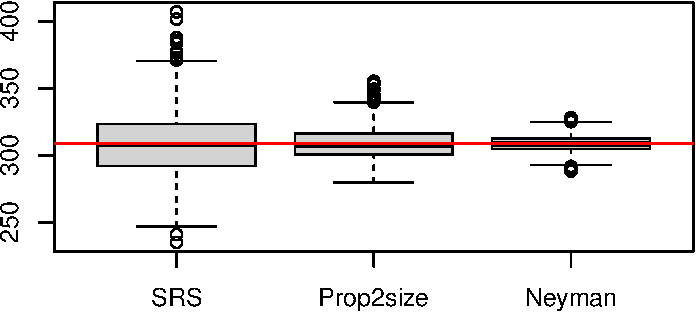
\includegraphics[keepaspectratio]{strata_files/figure-pdf/fig-agpop-acres82-compare-boxplot-1.pdf}}

}

\caption{\label{fig-agpop-acres82-compare-boxplot}Sampling distribution
of the mean under SRS, proportional, and Neyman allocation (acres82
strata, 2000 simulations)}

\end{figure}%

\begin{Shaded}
\begin{Highlighting}[]
\NormalTok{sim\_means }\OtherTok{\textless{}{-}} \FunctionTok{sapply}\NormalTok{(sim\_results\_str\_acres82, mean)}
\NormalTok{sim\_var }\OtherTok{\textless{}{-}} \FunctionTok{sapply}\NormalTok{(sim\_results\_str\_acres82, var)}
\NormalTok{sim\_var\_relative }\OtherTok{\textless{}{-}}\NormalTok{ sim\_var }\SpecialCharTok{/}\NormalTok{ sim\_var[}\DecValTok{1}\NormalTok{]}
\NormalTok{sim\_var\_reduction }\OtherTok{\textless{}{-}} \DecValTok{1} \SpecialCharTok{{-}}\NormalTok{ sim\_var\_relative}

\FunctionTok{data.frame}\NormalTok{(}
  \StringTok{"Mean"} \OtherTok{=}\NormalTok{ sim\_means,}
  \StringTok{"Variance"} \OtherTok{=}\NormalTok{ sim\_var,}
  \StringTok{"Relative Variance"} \OtherTok{=}\NormalTok{ sim\_var\_relative,}
  \StringTok{"Percentage of Variance Reduction"} \OtherTok{=}\NormalTok{ sim\_var\_reduction,}
  \AttributeTok{check.names =} \ConstantTok{FALSE}
\NormalTok{) }\SpecialCharTok{|\textgreater{}}
  \FunctionTok{gt}\NormalTok{(}\AttributeTok{rownames\_to\_stub =} \ConstantTok{TRUE}\NormalTok{) }\SpecialCharTok{|\textgreater{}}
  \FunctionTok{fmt\_number}\NormalTok{(}\AttributeTok{columns =} \FunctionTok{c}\NormalTok{(Mean, Variance), }\AttributeTok{decimals =} \DecValTok{1}\NormalTok{) }\SpecialCharTok{|\textgreater{}}
  \FunctionTok{fmt\_percent}\NormalTok{(}\AttributeTok{columns =} \FunctionTok{c}\NormalTok{(}\StringTok{\textasciigrave{}}\AttributeTok{Percentage of Variance Reduction}\StringTok{\textasciigrave{}}\NormalTok{), }\AttributeTok{decimals =} \DecValTok{2}\NormalTok{) }\SpecialCharTok{|\textgreater{}}
  \FunctionTok{fmt\_number}\NormalTok{(}\AttributeTok{columns =} \FunctionTok{c}\NormalTok{(}\StringTok{\textasciigrave{}}\AttributeTok{Relative Variance}\StringTok{\textasciigrave{}}\NormalTok{), }\AttributeTok{decimals =} \DecValTok{3}\NormalTok{)}
\end{Highlighting}
\end{Shaded}

\begin{table}

\caption{\label{tbl-agpop-acres82-compare-methods}Simulated mean,
variance, and variance reduction by allocation method (acres82 strata)}

\centering{

\normalsize
\begin{gtfit}{\linewidth}{l|rrrr}
\toprule
 & Mean & Variance & Relative Variance & Percentage of Variance Reduction \\ 
\midrule\addlinespace[2.5pt]
SRS & 308.5 & 537.1 & 1.000 & 0.00\% \\ 
Prop2size & 309.2 & 138.3 & 0.257 & 74.26\% \\ 
Neyman & 308.7 & 34.9 & 0.065 & 93.50\% \\ 
\bottomrule
\end{gtfit}

}

\end{table}%

The results are dramatic. Proportional allocation reduces the variance
by 74.3\%, again close to \(R^2 = 0.74\). Neyman allocation reduces it
by 93.5\%. The top stratum is both small and highly variable, so Neyman
allocation samples it heavily, just as dollar stratification samples the
largest loans. Stratifying by a variable that is highly correlated with
\(y\) is very powerful.

\section{\texorpdfstring{Interactive Demonstration: Stratification by
\texttt{acres82} or
\texttt{region}}{Interactive Demonstration: Stratification by acres82 or region}}\label{sec-app-stratification}

The simulation for this section runs as a standalone app:
\href{../shinylives_sampling/app-stratified.html}{Stratified Sampling}.
It opens in a new tab, together with its documentation and the full
\href{../shinylives_sampling/index.html}{list of apps}.

\bookmarksetup{startatroot}

\chapter{Ratio and Regression
Estimation}\label{ratio-and-regression-estimation}

\section{Introduction}\label{sec-ratio-formulas}

When auxiliary information (a variable \(x\)) is highly correlated with
our target variable of interest (\(y\)), we can use \textbf{ratio} or
\textbf{regression} estimation to improve precision without increasing
the sample size. We can also use auxiliary population structures to
adjust our estimates after the fact via \textbf{post-stratification}, or
estimate means for specific sub-populations (\textbf{domains}).

Throughout, \((x_i, y_i)\), \(i = 1, \ldots, n\), is an SRS of size
\(n\) from a population of \(N\) units, and \(\bar x_U\) (equivalently
\(t_x = N\bar x_U\)) is known. Each topic below has the same layout: a
\emph{theory} part that states the estimator, explains where it comes
from and gives its standard error, followed by worked examples with
data.

The topics are less separate than they look. The ratio, regression and
post-stratified estimators each fill in a prediction \(\hat y_i\) for
every unit of the population and average them; they differ only in the
auxiliary information used to form \(\hat y_i\), and a domain mean is
itself a ratio estimator. The regression and post-stratification
sections make this explicit, and the post-stratification section ends
with a table that puts the estimators side by side.

\section{Functions and packages for Analyzing
Data}\label{functions-and-packages-for-analyzing-data}

We begin by loading the necessary libraries, including \texttt{gt} for
formatting mathematical tables, and defining our custom functions for
Ratio, Regression, Domain, and Post-stratified estimation. We also
define a versatile \texttt{gt} helper to render our estimation outputs
cleanly.

\subsection{General functions for ratio and regression
estimation}\label{general-functions-for-ratio-and-regression-estimation}

The estimating functions used throughout this book (including
\texttt{reg\_est}, \texttt{ratio\_est}, \texttt{domain\_est},
\texttt{srs\_est}, and the \texttt{format\_est\_gt} table-formatting
helper used below) live in a single shared file,
\texttt{samplingestimate.r}, which we source below.

For post-stratification, we reuse the shared \texttt{str\_est()}
stratified estimator, but we plug in the expected sample sizes
\(n_h = n \times \frac{N_h}{N}\) instead of the actual observed random
\(n_h\).

The full source of \texttt{samplingestimate.r} is listed in
Appendix~\ref{sec-estimating-functions}.

\section{Ratio Estimation}\label{ratio-estimation}

\subsection{Theory}\label{sec-ratio-theory}

\subsubsection{The ratio estimator}\label{the-ratio-estimator}

For ratio estimation to apply, two quantities \(y_i\) and \(x_i\) must
be measured on each sample unit; \(x_i\) is often called an
\textbf{auxiliary variable} or \textbf{subsidiary variable}. In the
population of size \(N\), \[
t_y = \sum_{i=1}^N y_i, \qquad t_x = \sum_{i=1}^N x_i,
\] and their ratio is \[
B = \frac{t_y}{t_x} = \frac{\bar y_U}{\bar x_U}, \qquad \text{so that} \qquad \bar y_U = B\cdot\bar x_U .
\] Ratio and regression estimation both take advantage of the
correlation of \(x\) and \(y\) in the population; the higher the
correlation, the better they work.

If an SRS is taken, natural estimators for \(B\), \(t_y\) and
\(\bar y_U\) are \[
\boxed{\hat B = \frac{\bar y}{\bar x} = \frac{\sum_{i=1}^n y_i}{\sum_{i=1}^n x_i} = \frac{\hat t_y}{\hat t_x},
\qquad
\hat t_{yr} = \hat B\, t_x = N\,\hat{\bar y}_r,
\qquad
\hat{\bar y}_r = \hat B\, \bar x_U},
\] where \(t_x\) and \(\bar x_U\) are assumed \textbf{known}. This is
the key requirement for ratio estimation: we need to know the population
total or mean of the auxiliary variable \(x\) in advance. The ratio
estimator is slightly biased, but the bias is negligible when \(n\) is
large.

There is a useful way to read these formulas. Once \(\hat B\) is
estimated, form the \textbf{fitted value} \(\hat y_i = \hat B x_i\) for
every unit in the population, using its known \(x_i\). Summing or
averaging these over the population recovers the ratio estimators: \[
\hat t_{yr} = \sum_{i=1}^N \hat y_i = \hat B\, t_x ,
\qquad
\hat{\bar y}_r = \frac1N\sum_{i=1}^N \hat y_i = \hat B\, \bar x_U .
\]

Figure~\ref{fig-ratio-concept} shows this for a small population. The
grey points are the population, whose \(x_i\) are known, and the green
circles are an ordinary SRS. The red line \(\hat y = \hat B x\) is
fitted from the sample, and the red points are the fitted values for
every unit.

\begin{Shaded}
\begin{Highlighting}[]
\FunctionTok{plot\_ratio\_concept}\NormalTok{()}
\end{Highlighting}
\end{Shaded}

\begin{figure}[H]

\centering{

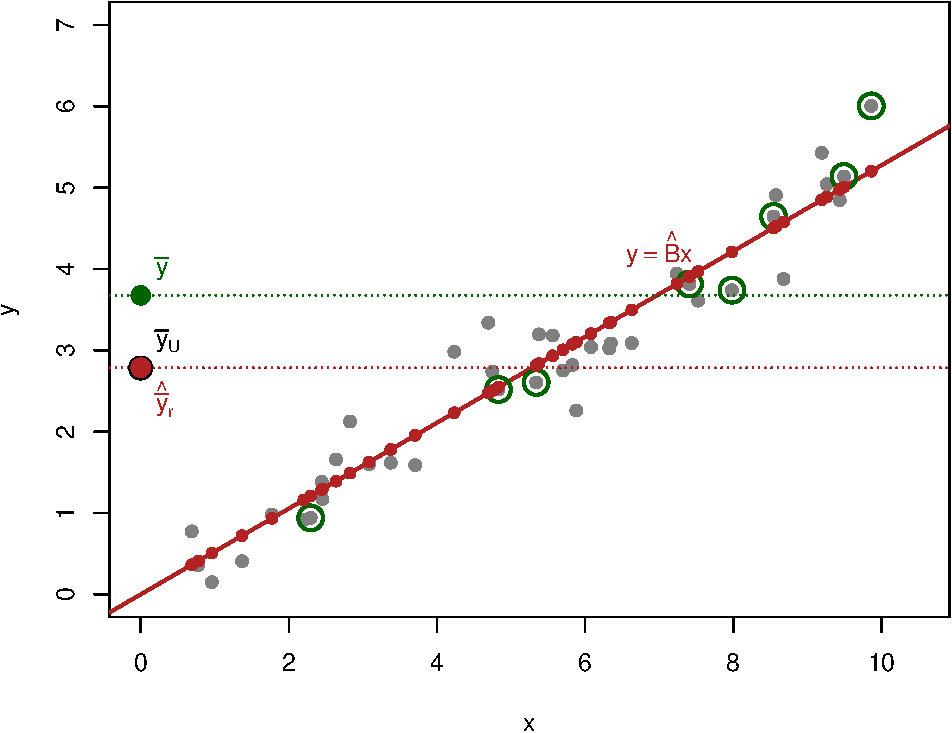
\includegraphics[width=0.7\linewidth,height=\textheight,keepaspectratio]{ratio_files/figure-pdf/fig-ratio-concept-1.pdf}

}

\caption{\label{fig-ratio-concept}Illustration of the benefits of ratio
estimation. Grey: the population. Green circles: an SRS. Red: the line
fitted from the sample and the fitted values for every unit.}

\end{figure}%

This sample happens to have \(\bar x > \bar x_U\), so the naive
\(\bar y\) (green) lands well above \(\bar y_U\). The ratio estimator
corrects for that through the known \(\bar x_U\): it is the height of
the red line at \(x = \bar x_U\), so \(\hat{\bar y}_r\) (red) is close
to \(\bar y_U\) (black). Averaged over samples both are (essentially)
unbiased, but \(\hat{\bar y}_r\) varies far less.

\subsubsection{Where ratio estimation is
used}\label{where-ratio-estimation-is-used}

Ordinary SRS estimation of a mean or proportion is a special case of
ratio estimation, obtained by setting \(x_i = 1\) for every unit: then
\(\bar x_U = \bar x = 1\), \(t_x = N\), \(B = \bar y_U\) and
\(\hat B = \bar y\), so \(\hat{\bar y}_r = \bar y\) (including
\(\hat p\)) and \(\hat t_{yr} = N\bar y\).

Genuine ratio estimation needs an \(x\) whose population total is known
more easily than that of \(y\). Three typical situations:

\begin{itemize}
\tightlist
\item
  \textbf{Counting people.} Let \(x_i\) be the number of registered
  births in commune \(i\) of France and \(y_i\) the number of residents.
  The total number of births is known from administrative records, so
  \(\hat B = \hat t_y/\hat t_x\) estimates residents per birth, and
  \(\hat t_{yr} = \hat B\,t_x\) estimates the population of France. For
  example, if a sample of communes has \(\hat t_y = 2{,}037{,}615\)
  residents and \(\hat t_x = 71{,}866\) births, then
  \(\hat B = 2{,}037{,}615/71{,}866 = 28.35\) residents per birth, and
  with \(t_x = 1\) million births in all of France,
  \(\hat t_{yr} = 28.35 \times 1\text{ million} = 28.35\) million
  residents.
\item
  \textbf{Field yield.} Let \(y_i\) be the bushels of grain harvested in
  field \(i\) and \(x_i\) its acreage. Then \(B\) is the average yield
  in bushels per acre, \(\bar y_U\) the average yield per field and
  \(t_y\) the total yield. The total acreage \(t_x\) is usually easy to
  obtain from other records, even when \(t_y\) is not.
\item
  \textbf{The same quantity at an earlier time.} When the same quantity
  is measured at different times, an earlier measurement often makes an
  excellent auxiliary variable. If the 1987 acreage of every county is
  known but 1992 acreage is observed only for a sample of counties, let
  \(y_i\) be the 1992 farm acreage and \(x_i\) the 1987 farm acreage.
  This is the example used in the simulation study at the end of this
  chapter.
\end{itemize}

\subsubsection{Standard error of the ratio
estimator}\label{standard-error-of-the-ratio-estimator}

In large samples the bias of \(\hat{\bar y}_r\) is negligible relative
to its variance, so
\(\text{MSE}(\hat{\bar y}_r) \approx V(\hat{\bar y}_r)\). To understand
the variance, look at the estimation error, \[
\hat{\bar y}_r - \bar y_U = \frac{\bar y}{\bar x}\bar x_U - B\bar x_U = \frac{\bar x_U}{\bar x}\left(\bar y - B\bar x\right),
\] where the second form comes from factoring out \(\bar x_U/\bar x\).
Define the \textbf{population residual} of each element as its deviation
from the true population line, \[
d_i = y_i - B x_i \qquad (B = t_y/t_x).
\] Then \(\bar y - B\bar x\) is simply the sample mean \(\bar d\) of
these residuals, so the error of the estimator is the scaled sample mean
of the residuals. Squaring and taking expectations, \[
\text{MSE}(\hat{\bar y}_r) \approx \left(\frac{\bar x_U}{\bar x}\right)^2 V(\bar d),
\qquad
V(\bar d) = \left(1 - \frac nN\right)\frac{S_d^2}{n},
\] because the \(d_i\) are fixed population values, so \(\bar d\) is an
ordinary sample mean under SRS.

In practice \(B\) is unknown, so the \(d_i\) cannot be computed. We
replace \(B\) by \(\hat B\) and use the \textbf{sample residuals} from
the fitted line, \[
e_i = y_i - \hat B x_i, \qquad s_e^2 = \frac{1}{n-1}\sum_{i=1}^n e_i^2 .
\] Substituting \(s_e^2\) for the unknown \(S_d^2\) gives the variance
estimators \[
\boxed{\begin{aligned}
\hat V(\hat B) &= \frac{1}{\bar x^2}\left(1 - \frac nN\right)\frac{s_e^2}{n}, \\
\hat V(\hat{\bar y}_r) &= \bar x_U^2\,\hat V(\hat B) = \left(\frac{\bar x_U}{\bar x}\right)^2\left(1 - \frac nN\right)\frac{s_e^2}{n}, \\
\hat V(\hat t_{yr}) &= N^2\,\hat V(\hat{\bar y}_r)
\end{aligned}}
\] For samples that are large enough (typically \(n > 30\)) the sampling
distributions are approximately normal, and approximate 95\% intervals
are \(\hat B \pm t_{0.975,\,n-1}\,\text{SE}(\hat B)\) for the ratio, and
the same form for the mean and the total.

The sample residual \(e_i\) is the vertical distance from the point
\((x_i, y_i)\) to the fitted line through the origin, \(y = \hat B x\).
No centring appears in \(s_e^2\) because \(\hat B = \bar y/\bar x\)
forces \(\sum_i e_i = \sum_i y_i - \hat B\sum_i x_i = 0\) exactly, so
the residuals already average to zero; the divisor is \(n-1\) for the
one parameter \(\hat B\) estimated from the sample. Compare the variance
with the SRS one, \(\left(1-\frac nN\right)s_y^2/n\): ratio estimation
replaces the scatter of \(y\) about \(\bar y\) by the scatter about the
line. That is the whole source of the gain, and the whole risk, since an
\(x\) that predicts \(y\) poorly gives \(s_e^2 > s_y^2\) and a
\emph{less} precise estimate than the plain sample mean.

\subsubsection{When does ratio estimation
help?}\label{when-does-ratio-estimation-help}

Let \(R\) be the population Pearson correlation of \(x\) and \(y\), \[
R = \frac{\sum_{i=1}^N (x_i - \bar x_U)(y_i - \bar y_U)}{(N-1)S_xS_y}.
\] Comparing \(\text{MSE}(\hat{\bar y}_r)\) with
\(\text{MSE}(\bar y) = \left(1 - \frac nN\right)S_y^2/n\) shows that \[
\text{MSE}(\hat{\bar y}_r) \le \text{MSE}(\bar y)
\quad\Longleftrightarrow\quad
R \ge \frac{B S_x}{2 S_y} = \frac{\text{CV}(x)}{2\,\text{CV}(y)} .
\] If the coefficients of variation of \(x\) and \(y\) are roughly
equal, ratio estimation pays off whenever the correlation between \(x\)
and \(y\) exceeds \(1/2\).

The gain can be summarized, analogously to \(R^2\) for stratification,
by \[
\frac{\text{MSE}(\hat{\bar y}_r)}{\text{MSE}(\bar y)} \approx \frac{S_d^2}{S_y^2}
\qquad\Longrightarrow\qquad
1 - \frac{S_d^2}{S_y^2}\ \text{is the proportion of variance removed.}
\] This is not exactly the \(R^2\) of fitting the linear model
\(y = Bx\), because \(\hat B\) is not a least-squares estimate of \(B\),
but it carries similar information about how much variance ratio
estimation removes.

\subsection{Example: Population of France (by
hand)}\label{example-population-of-france-by-hand}

This toy version of the France population example demonstrates the
mechanics of ratio estimation, using a sample of \(n = 5\) out of
\(N = 8\) communes. We observe \(x_i\) = registered births and \(y_i\) =
residents, both in thousands:

{\def\LTcaptype{none} % do not increment counter
\begin{longtable}[]{@{}
  >{\raggedright\arraybackslash}p{(\linewidth - 10\tabcolsep) * \real{0.1667}}
  >{\raggedleft\arraybackslash}p{(\linewidth - 10\tabcolsep) * \real{0.1667}}
  >{\raggedleft\arraybackslash}p{(\linewidth - 10\tabcolsep) * \real{0.1667}}
  >{\raggedleft\arraybackslash}p{(\linewidth - 10\tabcolsep) * \real{0.1667}}
  >{\raggedleft\arraybackslash}p{(\linewidth - 10\tabcolsep) * \real{0.1667}}
  >{\raggedleft\arraybackslash}p{(\linewidth - 10\tabcolsep) * \real{0.1667}}@{}}
\toprule\noalign{}
\begin{minipage}[b]{\linewidth}\raggedright
Commune \(i\)
\end{minipage} & \begin{minipage}[b]{\linewidth}\raggedleft
\(x_i\) (000s)
\end{minipage} & \begin{minipage}[b]{\linewidth}\raggedleft
\(y_i\) (000s)
\end{minipage} & \begin{minipage}[b]{\linewidth}\raggedleft
\(\hat y_i = \hat B x_i\)
\end{minipage} & \begin{minipage}[b]{\linewidth}\raggedleft
\(e_i = y_i - \hat y_i\)
\end{minipage} & \begin{minipage}[b]{\linewidth}\raggedleft
\(e_i^2\)
\end{minipage} \\
\midrule\noalign{}
\endhead
\bottomrule\noalign{}
\endlastfoot
1 & 1 & 18 & 30 & −12 & 144 \\
2 & 2 & 78 & 60 & 18 & 324 \\
3 & 3 & 62 & 90 & −28 & 784 \\
4 & 4 & 132 & 120 & 12 & 144 \\
5 & 5 & 160 & 150 & 10 & 100 \\
\textbf{Sum} & \textbf{15} & \textbf{450} & \textbf{450} & \textbf{0} &
\textbf{1496} \\
\end{longtable}
}

Figure~\ref{fig-france-toy} shows the five communes, the fitted line
\(y = \hat Bx\) through the origin, and the residuals \(e_i\).

\begin{figure}

\centering{

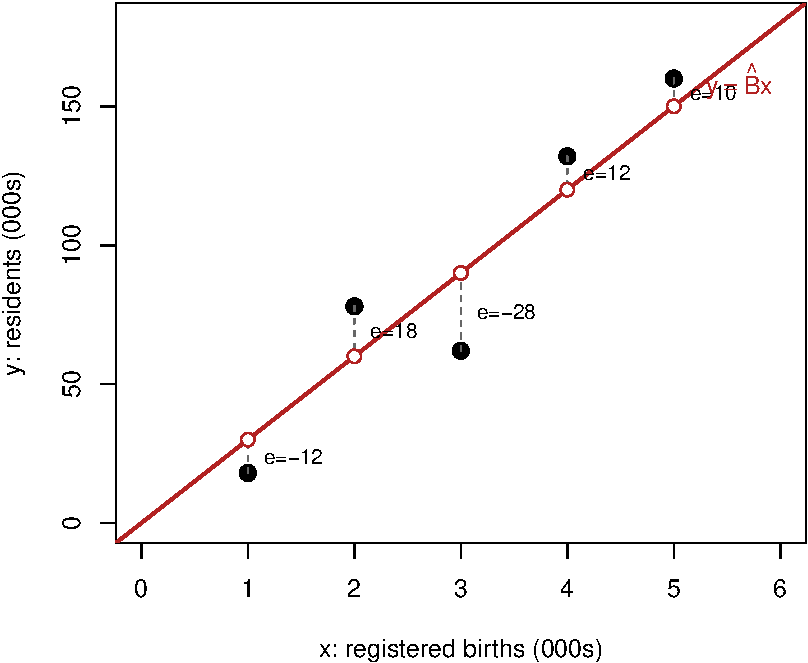
\includegraphics[width=0.55\linewidth,height=\textheight,keepaspectratio]{ratio_files/figure-pdf/fig-france-toy-1.pdf}

}

\caption{\label{fig-france-toy}The toy France example: residents against
registered births for the \(n = 5\) sampled communes, with the ratio
line \(y = \hat B x\) (red) and the residuals \(e_i\) (dashed).}

\end{figure}%

The ratio estimate of the slope and the sample residual variance are \[
\hat B = \frac{\sum y_i}{\sum x_i} = \frac{450}{15} = 30,
\qquad
s_e^2 = \frac{\sum e_i^2}{n-1} = \frac{1496}{4} = 374 .
\] Assume the number of registered births is known from administrative
records to be \(t_x = 40\) (thousand) in all \(N = 8\) communes. Then
\(\bar x_U = t_x/N = 5\) (thousand), while the sample mean is only
\(\bar x = 3\) (thousand): we sampled smaller-than-average communes. The
estimates are \[
\hat{\bar y}_r = \hat B\bar x_U = 30(5) = 150 \text{ (thousand residents)},
\qquad
\text{SE}(\hat{\bar y}_r) = \sqrt{\left(1 - \frac58\right)\left(\frac53\right)^2\frac{374}{5}} = 8.827,
\] \[
\hat t_{yr} = \hat B\,t_x = 30(40) = 1200 \text{ (thousand)},
\] \[
\text{SE}(\hat t_{yr}) = \sqrt{\left(1 - \frac58\right)\left(\frac{40}{3}\right)^2\frac{374}{5}} = 70.616 \text{ (thousand)},
\] so a 95\% confidence interval for the total population is
\(1200 \pm 1.96(70.616) = [1061.6,\ 1338.4]\) thousand, that is,
\textbf{{[}1.062, 1.338{]} million} residents. For the slope,
\(\text{SE}(\hat B) = \sqrt{\left(1 - \frac58\right)\frac{374}{5\cdot 3^2}} = 1.765\).

\subsection{Example: Farm Acreage, 1992 from 1987
(agsrs.csv)}\label{sec-ratio-agsrs}

When the same quantity is measured at different times, an earlier
measurement often makes an excellent auxiliary variable. The Census of
Agriculture gives the 1987 farm acreage of every county, but suppose the
1992 acreage is known only for the SRS of \(n = 300\) counties in
\texttt{agsrs.csv}. Let \[
y_i = \text{farm acreage of county } i \text{ in 1992}, \qquad
x_i = \text{farm acreage of county } i \text{ in 1987}.
\] In 1987 a total of \(t_x = 964{,}470{,}625\) acres were devoted to
farms, so \(\bar x_U = 964{,}470{,}625/3078 = 313{,}343.3\) acres per
county, or \(313.3\) thousand acres in the units used here.

\begin{Shaded}
\begin{Highlighting}[]
\NormalTok{agsrs }\OtherTok{\textless{}{-}} \FunctionTok{acres\_in\_thousands}\NormalTok{(}\FunctionTok{read.csv}\NormalTok{(}\StringTok{"data/agsrs.csv"}\NormalTok{))}
\NormalTok{tx }\OtherTok{\textless{}{-}} \FloatTok{964470.625}                       \CommentTok{\# thousands of acres, all 3078 counties in 1987}
\NormalTok{res\_ag\_ratio }\OtherTok{\textless{}{-}} \FunctionTok{ratio\_est}\NormalTok{(agsrs}\SpecialCharTok{$}\NormalTok{acres92, agsrs}\SpecialCharTok{$}\NormalTok{acres87, }\AttributeTok{xbarU =}\NormalTok{ tx }\SpecialCharTok{/} \DecValTok{3078}\NormalTok{, }\AttributeTok{N =} \DecValTok{3078}\NormalTok{,}
                          \AttributeTok{estimate =} \StringTok{"mean"}\NormalTok{, }\AttributeTok{show.details =} \ConstantTok{FALSE}\NormalTok{)}\SpecialCharTok{$}\NormalTok{estimate}
\NormalTok{res\_ag\_srs   }\OtherTok{\textless{}{-}} \FunctionTok{srs\_est}\NormalTok{(agsrs}\SpecialCharTok{$}\NormalTok{acres92, }\AttributeTok{N =} \DecValTok{3078}\NormalTok{, }\AttributeTok{estimate =} \StringTok{"mean"}\NormalTok{, }\AttributeTok{show.details =} \ConstantTok{FALSE}\NormalTok{)}\SpecialCharTok{$}\NormalTok{estimate}
\NormalTok{Bhat\_ag }\OtherTok{\textless{}{-}} \FunctionTok{mean}\NormalTok{(agsrs}\SpecialCharTok{$}\NormalTok{acres92) }\SpecialCharTok{/} \FunctionTok{mean}\NormalTok{(agsrs}\SpecialCharTok{$}\NormalTok{acres87)}
\FunctionTok{c}\NormalTok{(}\AttributeTok{ybar =} \FunctionTok{mean}\NormalTok{(agsrs}\SpecialCharTok{$}\NormalTok{acres92), }\AttributeTok{xbar =} \FunctionTok{mean}\NormalTok{(agsrs}\SpecialCharTok{$}\NormalTok{acres87), }\AttributeTok{Bhat =}\NormalTok{ Bhat\_ag)}
\end{Highlighting}
\end{Shaded}

\begin{verbatim}
       ybar        xbar        Bhat 
297.8970467 301.9537233   0.9865652 
\end{verbatim}

\begin{Shaded}
\begin{Highlighting}[]
\NormalTok{res\_ag\_ratio }\SpecialCharTok{|\textgreater{}} \FunctionTok{format\_est\_gt}\NormalTok{(}\StringTok{"ratio\_mean"}\NormalTok{)}
\end{Highlighting}
\end{Shaded}

\begin{table}[H]
\normalsize
\begin{gtfit}{0.7\linewidth}{rrrr}
\toprule
\(\bar{y}_{r}\) & \(\mathrm{SE}(\bar{y}_{r})\) & 95\% CI Lower & 95\% CI Upper \\ 
\midrule\addlinespace[2.5pt]
309.13 & 1.80 & 305.59 & 312.68 \\ 
\bottomrule
\end{gtfit}
\end{table}

\begin{Shaded}
\begin{Highlighting}[]
\NormalTok{res\_ag\_srs }\SpecialCharTok{|\textgreater{}} \FunctionTok{format\_est\_gt}\NormalTok{(}\StringTok{"mean"}\NormalTok{)}
\end{Highlighting}
\end{Shaded}

\begin{table}[H]
\normalsize
\begin{gtfit}{0.7\linewidth}{rrrr}
\toprule
\(\bar{y}\) & \(\mathrm{SE}(\bar{y})\) & 95\% CI Lower & 95\% CI Upper \\ 
\midrule\addlinespace[2.5pt]
297.90 & 18.90 & 260.71 & 335.09 \\ 
\bottomrule
\end{gtfit}
\end{table}

From the sample, \(\bar y = 297.9\) and \(\bar x = 302\) thousand acres,
so \[
\hat B = \frac{\bar y}{\bar x} = 0.986565, \qquad
\hat{\bar y}_r = \hat B\,\bar x_U = 309.1, \qquad
\hat t_{yr} = \hat B\,t_x = 951,513 \text{ thousand acres}.
\] The plain SRS estimate of the total, \(N\bar y = 916,927\) thousand
acres, is quite different, because the sampled counties happened to have
\(\bar x\) a little below \(\bar x_U\). The ratio estimator corrects for
this, and its standard error, 1.8, is about a tenth of the SRS standard
error, 18.9.

\begin{Shaded}
\begin{Highlighting}[]
\FunctionTok{par}\NormalTok{(}\AttributeTok{mar =} \FunctionTok{c}\NormalTok{(}\DecValTok{4}\NormalTok{, }\DecValTok{4}\NormalTok{, }\FloatTok{0.5}\NormalTok{, }\FloatTok{0.5}\NormalTok{))}
\FunctionTok{plot}\NormalTok{(agsrs}\SpecialCharTok{$}\NormalTok{acres87, agsrs}\SpecialCharTok{$}\NormalTok{acres92, }\AttributeTok{pch =} \DecValTok{19}\NormalTok{, }\AttributeTok{col =} \FunctionTok{adjustcolor}\NormalTok{(}\StringTok{"grey30"}\NormalTok{, }\FloatTok{0.6}\NormalTok{), }\AttributeTok{las =} \DecValTok{1}\NormalTok{,}
     \AttributeTok{xlab =} \StringTok{"Farm acreage 1987 (thousands)"}\NormalTok{, }\AttributeTok{ylab =} \StringTok{"Farm acreage 1992 (thousands)"}\NormalTok{)}
\FunctionTok{abline}\NormalTok{(}\DecValTok{0}\NormalTok{, Bhat\_ag, }\AttributeTok{col =} \StringTok{"firebrick"}\NormalTok{, }\AttributeTok{lwd =} \DecValTok{2}\NormalTok{)}
\end{Highlighting}
\end{Shaded}

\begin{figure}[H]

\centering{

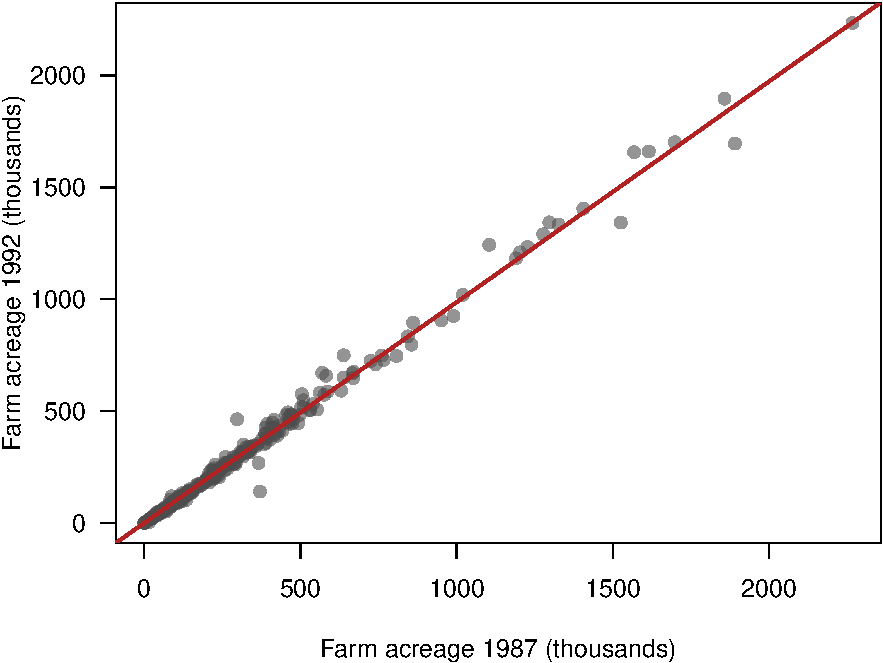
\includegraphics[width=0.6\linewidth,height=\textheight,keepaspectratio]{ratio_files/figure-pdf/fig-agsrs-acres8792-1.pdf}

}

\caption{\label{fig-agsrs-acres8792}1992 against 1987 farm acreage for
the SRS of 300 counties, with the ratio line \(y = \hat B x\) through
the origin. The spread about the line grows with \(x\).}

\end{figure}%

The points lie close to a line through the origin, and the variability
about the line \textbf{increases with \(x\)}. This pattern, with the
variance of \(y\) roughly proportional to \(x\), is exactly when ratio
estimation works best.

\subsection{Example: Cherry Trees
(cherry.csv)}\label{example-cherry-trees-cherry.csv}

We want to estimate the volume of wood in cherry trees using their
diameter as an auxiliary variable.

\subsubsection{Importing data}\label{importing-data}

First, let's load the data and look at the relationship between volume
and diameter.

\begin{Shaded}
\begin{Highlighting}[]
\NormalTok{cherry }\OtherTok{\textless{}{-}} \FunctionTok{read.csv}\NormalTok{(}\StringTok{"data/cherry.csv"}\NormalTok{, }\AttributeTok{header =}\NormalTok{ T)}
\FunctionTok{head}\NormalTok{(cherry) }\SpecialCharTok{|\textgreater{}} \FunctionTok{gt}\NormalTok{()}
\end{Highlighting}
\end{Shaded}

\begin{table}

\caption{\label{tbl-cherry-sample-data}Sample data: cherry tree volume
and diameter}

\centering{

\normalsize
\begin{gtfit}{\linewidth}{rrr}
\toprule
diameter & height & volume \\ 
\midrule\addlinespace[2.5pt]
8.3 & 70 & 10.3 \\ 
8.6 & 65 & 10.3 \\ 
8.8 & 63 & 10.2 \\ 
10.5 & 72 & 16.4 \\ 
10.7 & 81 & 18.8 \\ 
10.8 & 83 & 19.7 \\ 
\bottomrule
\end{gtfit}

}

\end{table}%

A scatter plot of volume against diameter shows whether the points lie
close to a line through the origin.

\begin{Shaded}
\begin{Highlighting}[]
\FunctionTok{plot}\NormalTok{(cherry}\SpecialCharTok{$}\NormalTok{volume }\SpecialCharTok{\textasciitilde{}}\NormalTok{ cherry}\SpecialCharTok{$}\NormalTok{diameter, }\AttributeTok{main =} \StringTok{"Volume vs Diameter"}\NormalTok{)}
\end{Highlighting}
\end{Shaded}

\begin{figure}[H]

\centering{

\pandocbounded{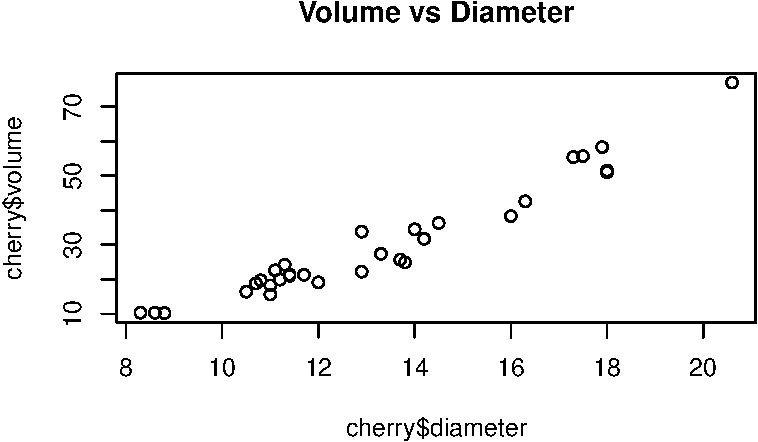
\includegraphics[keepaspectratio]{ratio_files/figure-pdf/fig-cherry-volume-diameter-1.pdf}}

}

\caption{\label{fig-cherry-volume-diameter}Cherry tree volume
vs.~diameter}

\end{figure}%

Fitting the linear model with the intercept forced to zero, \(y = Bx\),
summarizes how strongly volume is related to diameter.

\begin{Shaded}
\begin{Highlighting}[]
\FunctionTok{anova}\NormalTok{(}\FunctionTok{lm}\NormalTok{(cherry}\SpecialCharTok{$}\NormalTok{volume }\SpecialCharTok{\textasciitilde{}} \DecValTok{0} \SpecialCharTok{+}\NormalTok{ cherry}\SpecialCharTok{$}\NormalTok{diameter))}
\end{Highlighting}
\end{Shaded}

\begin{verbatim}
Analysis of Variance Table

Response: cherry$volume
                Df Sum Sq Mean Sq F value    Pr(>F)    
cherry$diameter  1  33622   33622  373.12 < 2.2e-16 ***
Residuals       30   2703      90                      
---
Signif. codes:  0 '***' 0.001 '**' 0.01 '*' 0.05 '.' 0.1 ' ' 1
\end{verbatim}

\textbf{Output Note:} The plot and the linear model output (which forces
a 0 intercept) confirm a very strong relationship, making this a prime
candidate for Ratio estimation.

\subsubsection{SRS estimate}\label{srs-estimate}

To establish a baseline, we first estimate the mean and total volume
using standard Simple Random Sampling (ignoring the auxiliary variable).

\begin{Shaded}
\begin{Highlighting}[]
\NormalTok{N }\OtherTok{\textless{}{-}} \DecValTok{2967}
\DocumentationTok{\#\# estimating the mean of volume}
\NormalTok{res\_srs\_vol }\OtherTok{\textless{}{-}} \FunctionTok{srs\_est}\NormalTok{(cherry}\SpecialCharTok{$}\NormalTok{volume, }\AttributeTok{N =}\NormalTok{ N, }\AttributeTok{estimate =} \StringTok{"mean"}\NormalTok{, }\AttributeTok{show.details =} \ConstantTok{FALSE}\NormalTok{)}
\NormalTok{srs\_mean\_vol\_raw }\OtherTok{\textless{}{-}}\NormalTok{ res\_srs\_vol}\SpecialCharTok{$}\NormalTok{estimate}
\NormalTok{srs\_mean\_vol\_raw }\SpecialCharTok{|\textgreater{}} \FunctionTok{format\_est\_gt}\NormalTok{(}\StringTok{"mean"}\NormalTok{)}
\end{Highlighting}
\end{Shaded}

\begin{table}[H]
\normalsize
\begin{gtfit}{0.7\linewidth}{rrrr}
\toprule
\(\bar{y}\) & \(\mathrm{SE}(\bar{y})\) & 95\% CI Lower & 95\% CI Upper \\ 
\midrule\addlinespace[2.5pt]
30.17 & 2.94 & 24.17 & 36.17 \\ 
\bottomrule
\end{gtfit}
\end{table}

\begin{Shaded}
\begin{Highlighting}[]
\DocumentationTok{\#\# estimating the total of volume}
\NormalTok{res\_srs\_total\_vol }\OtherTok{\textless{}{-}} \FunctionTok{srs\_est}\NormalTok{(cherry}\SpecialCharTok{$}\NormalTok{volume, }\AttributeTok{N =}\NormalTok{ N, }\AttributeTok{estimate =} \StringTok{"total"}\NormalTok{, }\AttributeTok{show.details =} \ConstantTok{FALSE}\NormalTok{)}
\NormalTok{srs\_total\_vol\_raw }\OtherTok{\textless{}{-}}\NormalTok{ res\_srs\_total\_vol}\SpecialCharTok{$}\NormalTok{estimate}
\NormalTok{srs\_total\_vol\_raw }\SpecialCharTok{|\textgreater{}} \FunctionTok{format\_est\_gt}\NormalTok{(}\StringTok{"total"}\NormalTok{)}
\end{Highlighting}
\end{Shaded}

\begin{table}[H]
\normalsize
\begin{gtfit}{0.7\linewidth}{rrrr}
\toprule
\(\hat{t}\) & \(\mathrm{SE}(\hat{t})\) & 95\% CI Lower & 95\% CI Upper \\ 
\midrule\addlinespace[2.5pt]
89,517.26 & 8,713.67 & 71,721.58 & 107,312.94 \\ 
\bottomrule
\end{gtfit}
\end{table}

\textbf{Output Note:} Under SRS, the standard error for the mean volume
is 2.94.

\subsubsection{Ratio Estimation Using the
Function}\label{ratio-estimation-using-the-function}

We calculate the ratio \(\hat{B} = \overline{y}/\overline{x}\); the
function's \texttt{\$table} shows the row-level working values \(x_i\),
\(y_i\), fitted \(\hat{y}_i = \hat{B}x_i\), residuals
\(e_i = y_i - \hat{y}_i\), and \(e_i^2\) (with a Sum row and a footnote
giving \(\hat B\) and \(s_e^2\)), so we no longer need to build this
table by hand.

\begin{Shaded}
\begin{Highlighting}[]
\NormalTok{ydata }\OtherTok{\textless{}{-}}\NormalTok{ cherry}\SpecialCharTok{$}\NormalTok{volume}
\NormalTok{xdata }\OtherTok{\textless{}{-}}\NormalTok{ cherry}\SpecialCharTok{$}\NormalTok{diameter}
\NormalTok{N }\OtherTok{\textless{}{-}} \DecValTok{2967}

\NormalTok{res\_ratio\_model }\OtherTok{\textless{}{-}} \FunctionTok{ratio\_est}\NormalTok{(ydata, xdata, }\AttributeTok{N =}\NormalTok{ N, }\AttributeTok{estimate =} \StringTok{"model"}\NormalTok{)}
\NormalTok{res\_ratio\_model}\SpecialCharTok{$}\NormalTok{table}
\end{Highlighting}
\end{Shaded}

\begin{table}[H]
\caption*{
{\large  Ratio Estimation: Working Table\normalsize } \\ 
{\normalsize  \(n = 31\)\normalsize }
} 
\normalsize
\begin{gtfit}{\linewidth}{>{\raggedright\arraybackslash}p{\dimexpr 30.00pt -2\tabcolsep-1.5\arrayrulewidth}>{\raggedleft\arraybackslash}p{\dimexpr 75.00pt -2\tabcolsep-1.5\arrayrulewidth}>{\raggedleft\arraybackslash}p{\dimexpr 75.00pt -2\tabcolsep-1.5\arrayrulewidth}>{\raggedleft\arraybackslash}p{\dimexpr 75.00pt -2\tabcolsep-1.5\arrayrulewidth}>{\raggedleft\arraybackslash}p{\dimexpr 75.00pt -2\tabcolsep-1.5\arrayrulewidth}>{\raggedleft\arraybackslash}p{\dimexpr 75.00pt -2\tabcolsep-1.5\arrayrulewidth}}
\toprule
\(i\) & \(y_i\) & \(x_i\) & \(\hat y_i\)\textsuperscript{\textit{1}} & \(e_i\) & \(e_i^2\) \\ 
\midrule\addlinespace[2.5pt]
1 & 10.30 & 8.30 & 18.90 & -8.60 & 73.99 \\ 
2 & 10.30 & 8.60 & 19.59 & -9.29 & 86.21 \\ 
3 & 10.20 & 8.80 & 20.04 & -9.84 & 96.84 \\ 
4 & 16.40 & 10.50 & 23.91 & -7.51 & 56.43 \\ 
5 & 18.80 & 10.70 & 24.37 & -5.57 & 31.00 \\ 
6 & 19.70 & 10.80 & 24.60 & -4.90 & 23.96 \\ 
... & ... & ... & ... & ... & ... \\ 
{\bfseries Sum} & {\bfseries 935.30} & {\bfseries 410.70} & {\bfseries 935.30} & {\bfseries 0.00} & {\bfseries 2,821.59} \\ 
\bottomrule
\end{gtfit}
\begin{minipage}{\linewidth}
\vspace{.05em}
\textsuperscript{\textit{1}}\(\hat B = \sum_i y_i / \sum_i x_i = 2.28\), \(\hat y_i = \hat B\, x_i\), \(s_e^2 = 94.05\).\\
\(\hat B = \dfrac{\sum_i y_i}{\sum_i x_i} = \dfrac{935.30}{410.70} = 2.28\)\\
\(\mathrm{SE}(\hat B) = \dfrac{1}{\bar x}\sqrt{\left(1-\dfrac{n}{N}\right)\dfrac{s_e^2}{n}} = \dfrac{1}{13.25}\sqrt{\left(1-\dfrac{31}{2967}\right)\dfrac{94.05}{31}} = 0.13\)\\
\end{minipage}
\end{table}

We plot the data again, now with the fitted line \(y = \hat B x\)
through the origin.

\begin{Shaded}
\begin{Highlighting}[]
\FunctionTok{plot}\NormalTok{(cherry}\SpecialCharTok{$}\NormalTok{volume }\SpecialCharTok{\textasciitilde{}}\NormalTok{ cherry}\SpecialCharTok{$}\NormalTok{diameter, }\AttributeTok{main=}\StringTok{"Ratio Estimation Fit"}\NormalTok{)}
\FunctionTok{abline}\NormalTok{(}\AttributeTok{a =} \DecValTok{0}\NormalTok{, }\AttributeTok{b =}\NormalTok{ res\_ratio\_model}\SpecialCharTok{$}\NormalTok{estimate[}\StringTok{"Est."}\NormalTok{], }\AttributeTok{col=}\StringTok{"blue"}\NormalTok{, }\AttributeTok{lwd=}\DecValTok{2}\NormalTok{)}
\end{Highlighting}
\end{Shaded}

\begin{figure}[H]

\centering{

\pandocbounded{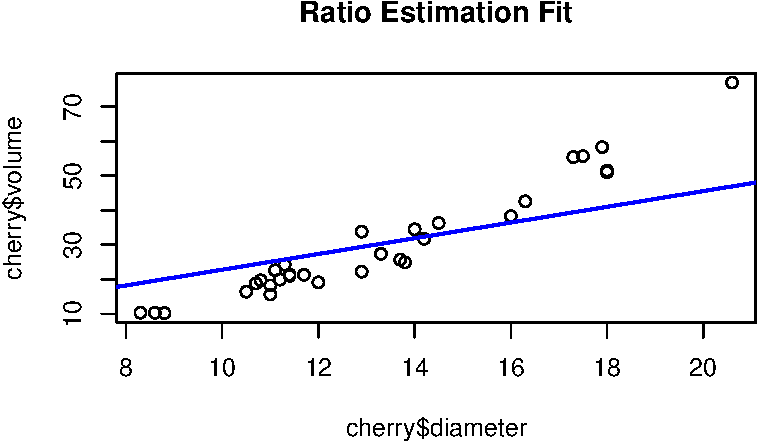
\includegraphics[keepaspectratio]{ratio_files/figure-pdf/fig-cherry-ratio-fit-1.pdf}}

}

\caption{\label{fig-cherry-ratio-fit}Cherry tree volume vs.~diameter
with the fitted ratio line}

\end{figure}%

\textbf{Output Note:} The blue line represents our estimated ratio
\(\hat{B} \approx 2.28\). The working table above shows the individual
residuals used to estimate \(s_e^2\).

\begin{Shaded}
\begin{Highlighting}[]
\NormalTok{B\_v2d }\OtherTok{\textless{}{-}}\NormalTok{ res\_ratio\_model}\SpecialCharTok{$}\NormalTok{estimate}
\NormalTok{B\_v2d }\SpecialCharTok{|\textgreater{}} \FunctionTok{format\_est\_gt}\NormalTok{(}\StringTok{"ratio"}\NormalTok{)}
\end{Highlighting}
\end{Shaded}

\begin{table}[H]
\normalsize
\begin{gtfit}{0.7\linewidth}{rrrr}
\toprule
\(\hat{B}\) & \(\mathrm{SE}(\hat{B})\) & 95\% CI Lower & 95\% CI Upper \\ 
\midrule\addlinespace[2.5pt]
2.28 & 0.13 & 2.01 & 2.54 \\ 
\bottomrule
\end{gtfit}
\end{table}

\textbf{Output Note:} The ratio \(\hat{B}\) is estimated at 2.277 with a
standard error of 0.1308.

\paragraph{Estimating the mean volume of
wood}\label{estimating-the-mean-volume-of-wood}

If we know the true total of the population diameters is 41,835, we can
derive the population mean diameter \(\overline{x}_{\text{U}}\) and pass
it as \texttt{xbarU} with \texttt{estimate\ =\ "mean"}.

\begin{Shaded}
\begin{Highlighting}[]
\NormalTok{mean\_diameters }\OtherTok{\textless{}{-}} \DecValTok{41835} \SpecialCharTok{/}\NormalTok{ N}
\NormalTok{res\_ratio\_mean }\OtherTok{\textless{}{-}} \FunctionTok{ratio\_est}\NormalTok{(ydata, xdata, }\AttributeTok{xbarU =}\NormalTok{ mean\_diameters, }\AttributeTok{N =}\NormalTok{ N, }\AttributeTok{estimate =} \StringTok{"mean"}\NormalTok{)}
\NormalTok{res\_ratio\_mean}\SpecialCharTok{$}\NormalTok{table}
\end{Highlighting}
\end{Shaded}

\begin{table}[H]
\caption*{
{\large  Ratio Estimation: Working Table\normalsize } \\ 
{\normalsize  \(n = 31\)\normalsize }
} 
\normalsize
\begin{gtfit}{\linewidth}{>{\raggedright\arraybackslash}p{\dimexpr 30.00pt -2\tabcolsep-1.5\arrayrulewidth}>{\raggedleft\arraybackslash}p{\dimexpr 75.00pt -2\tabcolsep-1.5\arrayrulewidth}>{\raggedleft\arraybackslash}p{\dimexpr 75.00pt -2\tabcolsep-1.5\arrayrulewidth}>{\raggedleft\arraybackslash}p{\dimexpr 75.00pt -2\tabcolsep-1.5\arrayrulewidth}>{\raggedleft\arraybackslash}p{\dimexpr 75.00pt -2\tabcolsep-1.5\arrayrulewidth}>{\raggedleft\arraybackslash}p{\dimexpr 75.00pt -2\tabcolsep-1.5\arrayrulewidth}}
\toprule
\(i\) & \(y_i\) & \(x_i\) & \(\hat y_i\)\textsuperscript{\textit{1}} & \(e_i\) & \(e_i^2\) \\ 
\midrule\addlinespace[2.5pt]
1 & 10.30 & 8.30 & 18.90 & -8.60 & 73.99 \\ 
2 & 10.30 & 8.60 & 19.59 & -9.29 & 86.21 \\ 
3 & 10.20 & 8.80 & 20.04 & -9.84 & 96.84 \\ 
4 & 16.40 & 10.50 & 23.91 & -7.51 & 56.43 \\ 
5 & 18.80 & 10.70 & 24.37 & -5.57 & 31.00 \\ 
6 & 19.70 & 10.80 & 24.60 & -4.90 & 23.96 \\ 
... & ... & ... & ... & ... & ... \\ 
{\bfseries Sum} & {\bfseries 935.30} & {\bfseries 410.70} & {\bfseries 935.30} & {\bfseries 0.00} & {\bfseries 2,821.59} \\ 
\bottomrule
\end{gtfit}
\begin{minipage}{\linewidth}
\vspace{.05em}
\textsuperscript{\textit{1}}\(\hat B = \sum_i y_i / \sum_i x_i = 2.28\), \(\hat y_i = \hat B\, x_i\), \(s_e^2 = 94.05\).\\
\(\bar y_r = \hat B\,\bar x_U = 2.28 \times 14.10 = 32.11\)\\
\(\mathrm{SE}(\bar y_r) = \mathrm{SE}(\hat B)\,\bar x_U = 0.13 \times 14.10 = 1.84\)\\
\end{minipage}
\end{table}

\begin{Shaded}
\begin{Highlighting}[]
\NormalTok{ratio\_mean\_volume\_raw }\OtherTok{\textless{}{-}}\NormalTok{ res\_ratio\_mean}\SpecialCharTok{$}\NormalTok{estimate}
\NormalTok{ratio\_mean\_volume\_raw }\SpecialCharTok{|\textgreater{}} \FunctionTok{format\_est\_gt}\NormalTok{(}\StringTok{"ratio\_mean"}\NormalTok{)}
\end{Highlighting}
\end{Shaded}

\begin{table}[H]
\normalsize
\begin{gtfit}{0.7\linewidth}{rrrr}
\toprule
\(\bar{y}_{r}\) & \(\mathrm{SE}(\bar{y}_{r})\) & 95\% CI Lower & 95\% CI Upper \\ 
\midrule\addlinespace[2.5pt]
32.11 & 1.84 & 28.34 & 35.88 \\ 
\bottomrule
\end{gtfit}
\end{table}

\paragraph{Estimating the total volume of
wood}\label{estimating-the-total-volume-of-wood}

Using \texttt{estimate\ =\ "total"} with the known population total
diameter gives the estimated population total volume directly.

\begin{Shaded}
\begin{Highlighting}[]
\NormalTok{t\_diameters }\OtherTok{\textless{}{-}} \DecValTok{41835}

\NormalTok{res\_ratio\_total }\OtherTok{\textless{}{-}} \FunctionTok{ratio\_est}\NormalTok{(ydata, xdata, }\AttributeTok{xbarU =}\NormalTok{ t\_diameters }\SpecialCharTok{/}\NormalTok{ N, }\AttributeTok{N =}\NormalTok{ N, }\AttributeTok{estimate =} \StringTok{"total"}\NormalTok{)}
\NormalTok{res\_ratio\_total}\SpecialCharTok{$}\NormalTok{table}
\end{Highlighting}
\end{Shaded}

\begin{table}[H]
\caption*{
{\large  Ratio Estimation: Working Table\normalsize } \\ 
{\normalsize  \(n = 31\)\normalsize }
} 
\normalsize
\begin{gtfit}{\linewidth}{>{\raggedright\arraybackslash}p{\dimexpr 30.00pt -2\tabcolsep-1.5\arrayrulewidth}>{\raggedleft\arraybackslash}p{\dimexpr 75.00pt -2\tabcolsep-1.5\arrayrulewidth}>{\raggedleft\arraybackslash}p{\dimexpr 75.00pt -2\tabcolsep-1.5\arrayrulewidth}>{\raggedleft\arraybackslash}p{\dimexpr 75.00pt -2\tabcolsep-1.5\arrayrulewidth}>{\raggedleft\arraybackslash}p{\dimexpr 75.00pt -2\tabcolsep-1.5\arrayrulewidth}>{\raggedleft\arraybackslash}p{\dimexpr 75.00pt -2\tabcolsep-1.5\arrayrulewidth}}
\toprule
\(i\) & \(y_i\) & \(x_i\) & \(\hat y_i\)\textsuperscript{\textit{1}} & \(e_i\) & \(e_i^2\) \\ 
\midrule\addlinespace[2.5pt]
1 & 10.30 & 8.30 & 18.90 & -8.60 & 73.99 \\ 
2 & 10.30 & 8.60 & 19.59 & -9.29 & 86.21 \\ 
3 & 10.20 & 8.80 & 20.04 & -9.84 & 96.84 \\ 
4 & 16.40 & 10.50 & 23.91 & -7.51 & 56.43 \\ 
5 & 18.80 & 10.70 & 24.37 & -5.57 & 31.00 \\ 
6 & 19.70 & 10.80 & 24.60 & -4.90 & 23.96 \\ 
... & ... & ... & ... & ... & ... \\ 
{\bfseries Sum} & {\bfseries 935.30} & {\bfseries 410.70} & {\bfseries 935.30} & {\bfseries 0.00} & {\bfseries 2,821.59} \\ 
\bottomrule
\end{gtfit}
\begin{minipage}{\linewidth}
\vspace{.05em}
\textsuperscript{\textit{1}}\(\hat B = \sum_i y_i / \sum_i x_i = 2.28\), \(\hat y_i = \hat B\, x_i\), \(s_e^2 = 94.05\).\\
\(\hat t = \hat B\,\bar x_U\,N = 2.28 \times 14.10 \times 2,967 = 95,272.16\)\\
\(\mathrm{SE}(\hat t) = \mathrm{SE}(\hat B)\,\bar x_U\,N = 0.13 \times 14.10 \times 2,967 = 5,471.43\)\\
\end{minipage}
\end{table}

\begin{Shaded}
\begin{Highlighting}[]
\NormalTok{ratio\_total\_volume }\OtherTok{\textless{}{-}}\NormalTok{ res\_ratio\_total}\SpecialCharTok{$}\NormalTok{estimate}
\NormalTok{ratio\_total\_volume }\SpecialCharTok{|\textgreater{}} \FunctionTok{format\_est\_gt}\NormalTok{(}\StringTok{"total"}\NormalTok{)}
\end{Highlighting}
\end{Shaded}

\begin{table}[H]
\normalsize
\begin{gtfit}{0.7\linewidth}{rrrr}
\toprule
\(\hat{t}\) & \(\mathrm{SE}(\hat{t})\) & 95\% CI Lower & 95\% CI Upper \\ 
\midrule\addlinespace[2.5pt]
95,272.16 & 5,471.43 & 84,098.00 & 106,446.32 \\ 
\bottomrule
\end{gtfit}
\end{table}

\paragraph{Percentage of Variance
Reduction}\label{percentage-of-variance-reduction}

How much did ratio estimation help compared to ignoring the auxiliary
variable?

\begin{Shaded}
\begin{Highlighting}[]
\NormalTok{variance\_reduction }\OtherTok{\textless{}{-}} \DecValTok{1} \SpecialCharTok{{-}}\NormalTok{ (ratio\_mean\_volume\_raw[}\StringTok{"S.E."}\NormalTok{] }\SpecialCharTok{/}\NormalTok{ srs\_mean\_vol\_raw[}\StringTok{"S.E."}\NormalTok{])}\SpecialCharTok{\^{}}\DecValTok{2}
\FunctionTok{unname}\NormalTok{(variance\_reduction)}
\end{Highlighting}
\end{Shaded}

\begin{verbatim}
[1] 0.6057237
\end{verbatim}

\textbf{Output Note:} Using the diameter as an auxiliary variable
reduced the variance of our estimate by 60.6\% compared to simple random
sampling.

\section{Regression Estimation}\label{regression-estimation}

\subsection{Theory}\label{sec-regression-theory}

\subsubsection{The linear model and the least-squares
fit}\label{the-linear-model-and-the-least-squares-fit}

Ratio estimation works best if the data are well fit by a straight line
\emph{through the origin}, with spread growing with \(x\). Sometimes
data instead appear evenly scattered about a straight line that does
\textbf{not} go through the origin, so that the usual straight-line
regression model applies, \[
y = B_0 + B_1 x .
\] In ratio estimation \(y_i = Bx_i + d_i\) with residual spread growing
with \(x\); in regression estimation \(y_i = B_0 + B_1x_i + d_i\) with
roughly constant spread.

\begin{figure}

\centering{

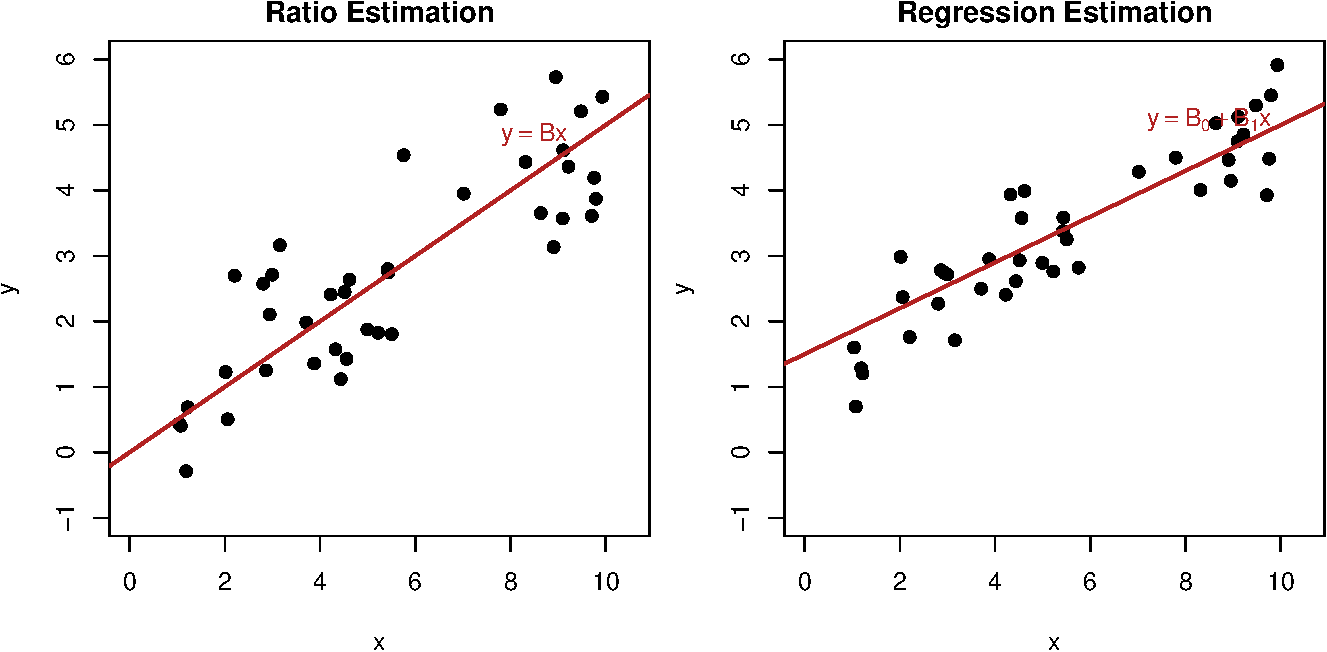
\includegraphics[width=0.9\linewidth,height=\textheight,keepaspectratio]{ratio_files/figure-pdf/fig-ratio-vs-reg-1.pdf}

}

\caption{\label{fig-ratio-vs-reg}Data suited to ratio estimation (left:
a line through the origin, with spread growing with \(x\)) and to
regression estimation (right: a line with a non-zero intercept and
constant spread).}

\end{figure}%

The ordinary least squares slope and intercept, from the sample, are \[
\hat B_1 = \frac{\sum_{i=1}^n (x_i - \bar x)(y_i - \bar y)}{\sum_{i=1}^n (x_i - \bar x)^2} = \frac{r\,s_y}{s_x},
\qquad
\hat B_0 = \bar y - \hat B_1\bar x ,
\] where \(r\) is the sample Pearson correlation coefficient of \(x\)
and \(y\).

\subsubsection{The regression estimator}\label{the-regression-estimator}

Assuming \(\bar x_U\) (or \(t_x\)) is known, the regression estimator of
the mean is the fitted line evaluated at \(\bar x_U\): \[
\boxed{\hat{\bar y}_{reg} = \hat B_0 + \hat B_1\bar x_U = \bar y + \hat B_1\left(\bar x_U - \bar x\right),
\qquad
\hat t_{reg} = N\hat{\bar y}_{reg} = N\hat B_0 + \hat B_1 t_x}.
\] Equivalently, averaging the fitted value
\(\hat y_i = \hat B_0 + \hat B_1 x_i\) over \emph{every} population unit
gives the same estimator, \[
\hat{\bar y}_{reg} = \frac1N\sum_{i=1}^N\left(\hat B_0 + \hat B_1 x_i\right) = \hat B_0 + \hat B_1\bar x_U .
\] This is a natural generalization of the ratio estimator
\(\hat{\bar y}_r = \frac1N\sum_{i=1}^N\hat B x_i\).

Figure~\ref{fig-reg-concept} illustrates it. The grey points are the
population and the green circles an ordinary SRS. The red line is fitted
from the sample, \(\hat y_i = \hat B_0 + \hat B_1x_i\) for every unit,
and the regression estimate is the average of the red points.

\begin{Shaded}
\begin{Highlighting}[]
\FunctionTok{plot\_reg\_concept}\NormalTok{()}
\end{Highlighting}
\end{Shaded}

\begin{figure}[H]

\centering{

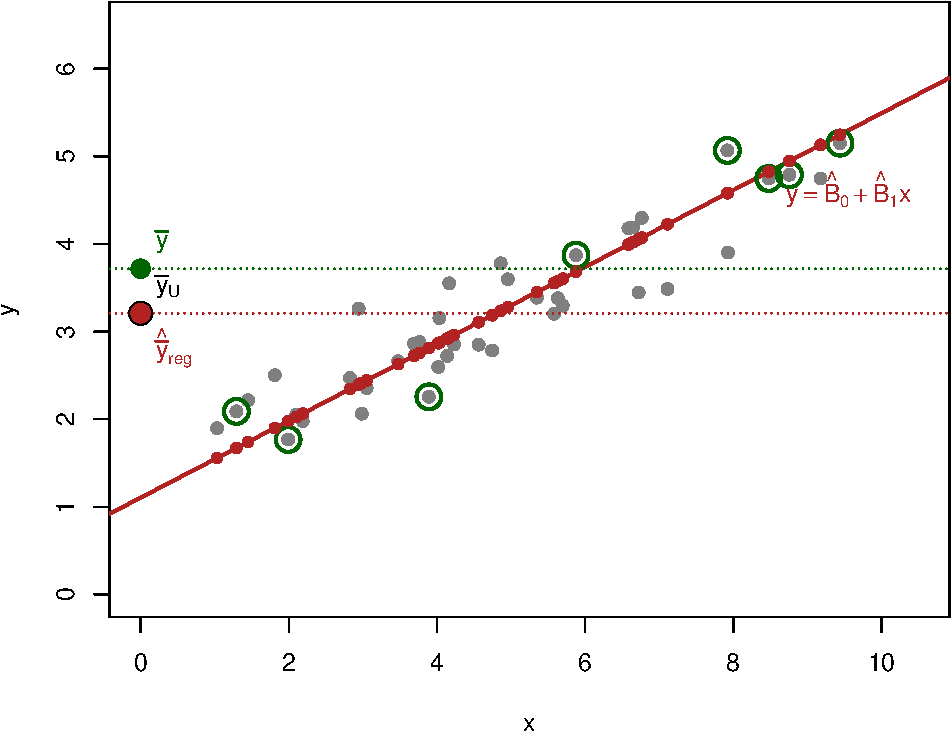
\includegraphics[width=0.7\linewidth,height=\textheight,keepaspectratio]{ratio_files/figure-pdf/fig-reg-concept-1.pdf}

}

\caption{\label{fig-reg-concept}Illustration of the benefits of
regression estimation. Grey: the population. Green circles: an SRS. Red:
the line fitted from the sample and the fitted values for every unit.}

\end{figure}%

The sampled \(x\)'s average above \(\bar x_U\), so the naive \(\bar y\)
(green) sits above \(\bar y_U\); the regression estimator shifts the fit
back to \(\bar x_U\) and lands on target, \(\hat{\bar y}_{reg}\) (red)
\(\approx \bar y_U\) (black). Both are essentially unbiased over
repeated samples, but \(\hat{\bar y}_{reg}\) is much less variable.

\subsubsection{Standard error of the regression
estimator}\label{standard-error-of-the-regression-estimator}

Let \(e_i = y_i - (\hat B_0 + \hat B_1 x_i)\) be the regression
residuals. The estimated variance uses the residual mean square of the
regression, \[
\boxed{\hat V(\hat{\bar y}_{reg}) = \left(1 - \frac nN\right)\frac{s_e^2}{n},
\qquad
s_e^2 = \frac{1}{n-2}\sum_{i=1}^n\left(y_i - \hat B_0 - \hat B_1 x_i\right)^2},
\] with \(\hat V(\hat t_{reg}) = N^2\hat V(\hat{\bar y}_{reg})\) and
95\% intervals using \(t_{0.975,\,n-2}\). Since
\(s_e^2 = s_y^2(1 - r^2)(n-1)/(n-2)\), the standard error is
approximately \[
\text{SE}(\hat{\bar y}_{reg}) \approx \sqrt{\left(1 - \frac nN\right)\frac1n\, s_y^2\left(1 - r^2\right)},
\] so the stronger the linear relationship, the smaller the SE.

The divisor is now \(n - 2\), since both \(\hat B_0\) and \(\hat B_1\)
are estimated. For the same data \(\sum_i e_i^2\) can only be smaller
here than under the ratio fit (the ratio line is the special case
\(\hat B_0 = 0\)), so the regression estimator is the safer of the two
whenever the relationship misses the origin, at the cost of one degree
of freedom. Note also that the factor \((\bar x_U/\bar x)^2\) is absent:
the fitted line is evaluated at \(\bar x_U\) directly, so no correction
for \(\bar x \neq \bar x_U\) is needed.

\subsection{Example: Cherry Trees
(cherry.csv)}\label{example-cherry-trees-cherry.csv-1}

When the relationship between \(y\) and \(x\) doesn't pass exactly
through the origin, we use Regression Estimation.

\subsubsection{Importing data}\label{importing-data-1}

We read the cherry data again. The known population total diameter,
\(t_x = 41{,}835\), over the \(N = 2967\) trees gives the population
mean diameter \(\bar x_U\) needed by the regression estimator.

\begin{Shaded}
\begin{Highlighting}[]
\NormalTok{cherry }\OtherTok{\textless{}{-}} \FunctionTok{read.csv}\NormalTok{(}\StringTok{"data/cherry.csv"}\NormalTok{, }\AttributeTok{header =}\NormalTok{ T)}
\NormalTok{ydata }\OtherTok{\textless{}{-}}\NormalTok{ cherry}\SpecialCharTok{$}\NormalTok{volume }
\NormalTok{xdata }\OtherTok{\textless{}{-}}\NormalTok{ cherry}\SpecialCharTok{$}\NormalTok{diameter}
\NormalTok{t\_diameters }\OtherTok{\textless{}{-}} \DecValTok{41835}
\NormalTok{xbarU }\OtherTok{\textless{}{-}}\NormalTok{ t\_diameters }\SpecialCharTok{/} \DecValTok{2967} 
\NormalTok{N }\OtherTok{\textless{}{-}} \DecValTok{2967}
\end{Highlighting}
\end{Shaded}

\subsubsection{Regression Estimation Using the
Function}\label{regression-estimation-using-the-function}

\paragraph{Fitting a linear regression
model}\label{fitting-a-linear-regression-model}

First fit the ordinary least squares line of volume on diameter. This
gives \(\hat B_0\) and \(\hat B_1\), together with the usual fit
summary, and shows how well a straight line describes the data.

\begin{Shaded}
\begin{Highlighting}[]
\NormalTok{n }\OtherTok{\textless{}{-}} \FunctionTok{length}\NormalTok{(ydata)}
\NormalTok{lmfit }\OtherTok{\textless{}{-}} \FunctionTok{lm}\NormalTok{(ydata }\SpecialCharTok{\textasciitilde{}}\NormalTok{ xdata)}
\NormalTok{lmfit\_gt }\OtherTok{\textless{}{-}} \FunctionTok{format\_lm\_gt}\NormalTok{(lmfit)}
\NormalTok{lmfit\_gt}\SpecialCharTok{$}\NormalTok{coef}
\end{Highlighting}
\end{Shaded}

\begin{table}[H]
\caption*{
{\large  Coefficient Estimates\normalsize }
} 
\normalsize
\begin{gtfit}{0.7\linewidth}{l|rrrr}
\toprule
 & Estimate & S.E. & t value & p value \\ 
\midrule\addlinespace[2.5pt]
(Intercept) & -36.9435 & 3.3651 & -10.9783 & 0.0000 \\ 
xdata & 5.0659 & 0.2474 & 20.4783 & 0.0000 \\ 
\bottomrule
\end{gtfit}
\end{table}

\begin{Shaded}
\begin{Highlighting}[]
\NormalTok{lmfit\_gt}\SpecialCharTok{$}\NormalTok{fit}
\end{Highlighting}
\end{Shaded}

\begin{table}[H]
\caption*{
{\large  Model Fit Summary\normalsize }
} 
\normalsize
\begin{gtfit}{0.7\linewidth}{rrrrr}
\toprule
\(R^2\) & Adj. \(R^2\) & \(\hat\sigma\) & F-statistic & p-value \\ 
\midrule\addlinespace[2.5pt]
0.9353 & 0.9331 & 4.2520 & 419.3603 & 0.0000 \\ 
\bottomrule
\end{gtfit}
\end{table}

The fitted line, which is not forced through the origin, is drawn over
the data.

\begin{Shaded}
\begin{Highlighting}[]
\FunctionTok{plot}\NormalTok{(xdata, ydata, }\AttributeTok{main=}\StringTok{"Linear Regression: Volume vs Diameter"}\NormalTok{)}
\FunctionTok{abline}\NormalTok{(lmfit, }\AttributeTok{col=}\StringTok{"green"}\NormalTok{, }\AttributeTok{lwd=}\DecValTok{2}\NormalTok{)}
\end{Highlighting}
\end{Shaded}

\begin{figure}[H]

\centering{

\pandocbounded{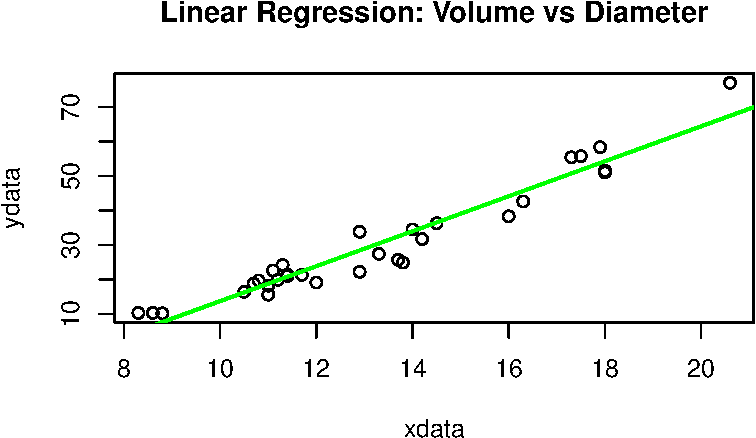
\includegraphics[keepaspectratio]{ratio_files/figure-pdf/fig-cherry-regression-fit-1.pdf}}

}

\caption{\label{fig-cherry-regression-fit}Cherry tree volume
vs.~diameter with the fitted regression line}

\end{figure}%

The function's \texttt{\$table} shows the row-level working values
\(x_i\), \(y_i\), fitted \(\hat{y}_i = \hat{B}_0 + \hat{B}_1 x_i\),
residuals \(e_i = y_i - \hat{y}_i\), and \(e_i^2\) (with a Sum row and a
footnote giving \(\hat B_0\), \(\hat B_1\), and \(s_e^2\)):

\begin{Shaded}
\begin{Highlighting}[]
\NormalTok{res\_reg\_model }\OtherTok{\textless{}{-}} \FunctionTok{reg\_est}\NormalTok{(ydata, xdata, }\AttributeTok{N =}\NormalTok{ N, }\AttributeTok{estimate =} \StringTok{"model"}\NormalTok{)}
\NormalTok{res\_reg\_model}\SpecialCharTok{$}\NormalTok{table}
\end{Highlighting}
\end{Shaded}

\begin{table}[H]
\caption*{
{\large  Regression Estimation: Working Table\normalsize } \\ 
{\normalsize  \(n = 31\)\normalsize }
} 
\normalsize
\begin{gtfit}{\linewidth}{>{\raggedright\arraybackslash}p{\dimexpr 30.00pt -2\tabcolsep-1.5\arrayrulewidth}>{\raggedleft\arraybackslash}p{\dimexpr 75.00pt -2\tabcolsep-1.5\arrayrulewidth}>{\raggedleft\arraybackslash}p{\dimexpr 75.00pt -2\tabcolsep-1.5\arrayrulewidth}>{\raggedleft\arraybackslash}p{\dimexpr 75.00pt -2\tabcolsep-1.5\arrayrulewidth}>{\raggedleft\arraybackslash}p{\dimexpr 75.00pt -2\tabcolsep-1.5\arrayrulewidth}>{\raggedleft\arraybackslash}p{\dimexpr 75.00pt -2\tabcolsep-1.5\arrayrulewidth}}
\toprule
\(i\) & \(y_i\) & \(x_i\) & \(\hat y_i\)\textsuperscript{\textit{1}} & \(e_i\) & \(e_i^2\) \\ 
\midrule\addlinespace[2.5pt]
1 & 10.30 & 8.30 & 5.10 & 5.20 & 27.01 \\ 
2 & 10.30 & 8.60 & 6.62 & 3.68 & 13.52 \\ 
3 & 10.20 & 8.80 & 7.64 & 2.56 & 6.57 \\ 
4 & 16.40 & 10.50 & 16.25 & 0.15 & 0.02 \\ 
5 & 18.80 & 10.70 & 17.26 & 1.54 & 2.37 \\ 
6 & 19.70 & 10.80 & 17.77 & 1.93 & 3.73 \\ 
... & ... & ... & ... & ... & ... \\ 
{\bfseries Sum} & {\bfseries 935.30} & {\bfseries 410.70} & {\bfseries 935.30} & {\bfseries 0.00} & {\bfseries 524.30} \\ 
\bottomrule
\end{gtfit}
\begin{minipage}{\linewidth}
\vspace{.05em}
\textsuperscript{\textit{1}}\(\hat B_0 = -36.94\), \(\hat B_1 = 5.07\), \(\hat y_i = \hat B_0 + \hat B_1 x_i\), \(s_e^2 = 18.08\).\\
\(\hat B_1 = \dfrac{\sum_i(x_i-\bar x)(y_i-\bar y)}{\sum_i(x_i-\bar x)^2} = \dfrac{1,496.64}{295.44} = 5.07\)\\
\(\mathrm{SE}(\hat B_1) = \sqrt{\dfrac{s_e^2}{\sum_i(x_i-\bar x)^2}} = \sqrt{\dfrac{18.08}{295.44}} = 0.25\)\\
\end{minipage}
\end{table}

\paragraph{Estimate the mean}\label{estimate-the-mean}

We compute the regression estimate \(\overline{y}_{reg}\) by passing
\texttt{xbarU} with \texttt{estimate\ =\ "mean"}.

\begin{Shaded}
\begin{Highlighting}[]
\NormalTok{res\_reg\_mean }\OtherTok{\textless{}{-}} \FunctionTok{reg\_est}\NormalTok{(ydata, xdata, }\AttributeTok{xbarU =}\NormalTok{ xbarU, }\AttributeTok{N =}\NormalTok{ N, }\AttributeTok{estimate =} \StringTok{"mean"}\NormalTok{)}
\NormalTok{res\_reg\_mean}\SpecialCharTok{$}\NormalTok{table}
\end{Highlighting}
\end{Shaded}

\begin{table}[H]
\caption*{
{\large  Regression Estimation: Working Table\normalsize } \\ 
{\normalsize  \(n = 31\)\normalsize }
} 
\normalsize
\begin{gtfit}{\linewidth}{>{\raggedright\arraybackslash}p{\dimexpr 30.00pt -2\tabcolsep-1.5\arrayrulewidth}>{\raggedleft\arraybackslash}p{\dimexpr 75.00pt -2\tabcolsep-1.5\arrayrulewidth}>{\raggedleft\arraybackslash}p{\dimexpr 75.00pt -2\tabcolsep-1.5\arrayrulewidth}>{\raggedleft\arraybackslash}p{\dimexpr 75.00pt -2\tabcolsep-1.5\arrayrulewidth}>{\raggedleft\arraybackslash}p{\dimexpr 75.00pt -2\tabcolsep-1.5\arrayrulewidth}>{\raggedleft\arraybackslash}p{\dimexpr 75.00pt -2\tabcolsep-1.5\arrayrulewidth}}
\toprule
\(i\) & \(y_i\) & \(x_i\) & \(\hat y_i\)\textsuperscript{\textit{1}} & \(e_i\) & \(e_i^2\) \\ 
\midrule\addlinespace[2.5pt]
1 & 10.30 & 8.30 & 5.10 & 5.20 & 27.01 \\ 
2 & 10.30 & 8.60 & 6.62 & 3.68 & 13.52 \\ 
3 & 10.20 & 8.80 & 7.64 & 2.56 & 6.57 \\ 
4 & 16.40 & 10.50 & 16.25 & 0.15 & 0.02 \\ 
5 & 18.80 & 10.70 & 17.26 & 1.54 & 2.37 \\ 
6 & 19.70 & 10.80 & 17.77 & 1.93 & 3.73 \\ 
... & ... & ... & ... & ... & ... \\ 
{\bfseries Sum} & {\bfseries 935.30} & {\bfseries 410.70} & {\bfseries 935.30} & {\bfseries 0.00} & {\bfseries 524.30} \\ 
\bottomrule
\end{gtfit}
\begin{minipage}{\linewidth}
\vspace{.05em}
\textsuperscript{\textit{1}}\(\hat B_0 = -36.94\), \(\hat B_1 = 5.07\), \(\hat y_i = \hat B_0 + \hat B_1 x_i\), \(s_e^2 = 18.08\).\\
\(\bar y_{reg} = \hat B_0+\hat B_1\bar x_U = -36.94 + 5.07 \times 14.10 = 34.49\)\\
\(\mathrm{SE}(\bar y_{reg}) = \sqrt{\left(1-\dfrac{n}{N}\right)\dfrac{s_e^2}{n}} = \sqrt{\left(1-\dfrac{31}{2967}\right)\dfrac{18.08}{31}} = 0.76\)\\
\end{minipage}
\end{table}

\begin{Shaded}
\begin{Highlighting}[]
\NormalTok{output\_reg }\OtherTok{\textless{}{-}}\NormalTok{ res\_reg\_mean}\SpecialCharTok{$}\NormalTok{estimate}
\NormalTok{output\_reg }\SpecialCharTok{|\textgreater{}} \FunctionTok{format\_est\_gt}\NormalTok{(}\StringTok{"reg\_mean"}\NormalTok{)}
\end{Highlighting}
\end{Shaded}

\begin{table}[H]
\normalsize
\begin{gtfit}{0.7\linewidth}{rrrr}
\toprule
\(\bar{y}_{reg}\) & \(\mathrm{SE}(\bar{y}_{reg})\) & 95\% CI Lower & 95\% CI Upper \\ 
\midrule\addlinespace[2.5pt]
34.49 & 0.76 & 32.93 & 36.04 \\ 
\bottomrule
\end{gtfit}
\end{table}

\textbf{Output Note:} The Regression estimate for the mean volume is
34.486 with a standard error of 0.7597.

\paragraph{Estimate the total}\label{estimate-the-total}

The estimate of the total follows by passing
\texttt{estimate\ =\ "total"}, which multiplies the estimated mean and
its standard error by \(N\).

\begin{Shaded}
\begin{Highlighting}[]
\NormalTok{reg\_total\_volume\_raw }\OtherTok{\textless{}{-}} \FunctionTok{reg\_est}\NormalTok{(ydata, xdata, }\AttributeTok{xbarU =}\NormalTok{ xbarU, }\AttributeTok{N =}\NormalTok{ N, }\AttributeTok{estimate =} \StringTok{"total"}\NormalTok{)}\SpecialCharTok{$}\NormalTok{estimate}
\NormalTok{reg\_total\_volume\_raw }\SpecialCharTok{|\textgreater{}} \FunctionTok{format\_est\_gt}\NormalTok{(}\StringTok{"reg\_total"}\NormalTok{)}
\end{Highlighting}
\end{Shaded}

\begin{table}[H]
\normalsize
\begin{gtfit}{0.7\linewidth}{rrrr}
\toprule
\(\hat{t}_{reg}\) & \(\mathrm{SE}(\hat{t}_{reg})\) & 95\% CI Lower & 95\% CI Upper \\ 
\midrule\addlinespace[2.5pt]
102,318.86 & 2,253.97 & 97,708.98 & 106,928.74 \\ 
\bottomrule
\end{gtfit}
\end{table}

\paragraph{Percentage of Variance
Reduction}\label{percentage-of-variance-reduction-1}

As for the ratio estimator, we compare the standard error of the
regression estimate with that of the SRS estimate:

\begin{Shaded}
\begin{Highlighting}[]
\NormalTok{reg\_mean\_volume\_raw }\OtherTok{\textless{}{-}}\NormalTok{ output\_reg}
\NormalTok{var\_reduction\_reg }\OtherTok{\textless{}{-}} \DecValTok{1} \SpecialCharTok{{-}}\NormalTok{ (reg\_mean\_volume\_raw[}\StringTok{"S.E."}\NormalTok{] }\SpecialCharTok{/}\NormalTok{ srs\_mean\_vol\_raw[}\StringTok{"S.E."}\NormalTok{])}\SpecialCharTok{\^{}}\DecValTok{2}
\FunctionTok{unname}\NormalTok{(var\_reduction\_reg)}
\end{Highlighting}
\end{Shaded}

\begin{verbatim}
[1] 0.9330895
\end{verbatim}

\textbf{Output Note:} The variance reduction for the regression
estimator is 93.3\%, much larger than the 60.6\% of the ratio estimator.
The fitted intercept, \(\hat B_0 = -36.94\), is far from zero: volume
grows faster than in proportion to diameter, so a line through the
origin fits poorly, while a straight line with an intercept fits well
over the range of the data.

\subsection{Example: Photo Counts of Dead
Trees}\label{example-photo-counts-of-dead-trees}

Aerial photographs are a cheap way to survey a large area (for example a
caribou herd), but they tend to \textbf{undercount} animals that are
hidden from view overhead. A more expensive, intensive ground count on a
subsample of plots gives accurate counts that can calibrate the photo
counts. Let \(x_i\) be the photo count and \(y_i\) the field count on
plot \(i\). Fitting a ratio or a regression line on the subsample of
plots that have both counts lets us correct the total photo count of the
\emph{entire} surveyed area, for example \(\hat t_{yr} = \hat B\,t_x\),
for the systematic undercounting bias.

To estimate the number of dead trees in an area, we divide the area into
100 square plots and count dead trees on photographs. We select an SRS
of 25 plots for exact field counts. We know the true mean photo count is
11.3.

The photo counts and the field counts of the 25 sampled plots are
entered below, and a straight line of field counts on photo counts is
fitted.

\begin{Shaded}
\begin{Highlighting}[]
\NormalTok{photocounts }\OtherTok{\textless{}{-}} \FunctionTok{c}\NormalTok{(}\DecValTok{10}\NormalTok{, }\DecValTok{12}\NormalTok{, }\DecValTok{7}\NormalTok{, }\DecValTok{13}\NormalTok{, }\DecValTok{13}\NormalTok{, }\DecValTok{6}\NormalTok{, }\DecValTok{17}\NormalTok{, }\DecValTok{16}\NormalTok{, }\DecValTok{15}\NormalTok{, }\DecValTok{10}\NormalTok{, }\DecValTok{14}\NormalTok{, }\DecValTok{12}\NormalTok{, }\DecValTok{10}\NormalTok{, }\DecValTok{5}\NormalTok{, }\DecValTok{12}\NormalTok{, }\DecValTok{10}\NormalTok{,}
                 \DecValTok{10}\NormalTok{, }\DecValTok{9}\NormalTok{, }\DecValTok{6}\NormalTok{, }\DecValTok{11}\NormalTok{, }\DecValTok{7}\NormalTok{, }\DecValTok{9}\NormalTok{, }\DecValTok{11}\NormalTok{, }\DecValTok{10}\NormalTok{, }\DecValTok{10}\NormalTok{)}

\NormalTok{fieldcounts }\OtherTok{\textless{}{-}} \FunctionTok{c}\NormalTok{(}\DecValTok{15}\NormalTok{, }\DecValTok{14}\NormalTok{, }\DecValTok{9}\NormalTok{, }\DecValTok{14}\NormalTok{, }\DecValTok{8}\NormalTok{, }\DecValTok{5}\NormalTok{, }\DecValTok{18}\NormalTok{, }\DecValTok{15}\NormalTok{, }\DecValTok{13}\NormalTok{, }\DecValTok{15}\NormalTok{, }\DecValTok{11}\NormalTok{, }\DecValTok{15}\NormalTok{, }\DecValTok{12}\NormalTok{, }\DecValTok{8}\NormalTok{, }\DecValTok{13}\NormalTok{,}
                 \DecValTok{9}\NormalTok{, }\DecValTok{11}\NormalTok{, }\DecValTok{12}\NormalTok{, }\DecValTok{9}\NormalTok{, }\DecValTok{12}\NormalTok{, }\DecValTok{13}\NormalTok{, }\DecValTok{11}\NormalTok{, }\DecValTok{10}\NormalTok{, }\DecValTok{9}\NormalTok{, }\DecValTok{8}\NormalTok{)}

\NormalTok{lmfit }\OtherTok{\textless{}{-}} \FunctionTok{lm}\NormalTok{(fieldcounts }\SpecialCharTok{\textasciitilde{}}\NormalTok{ photocounts)}
\NormalTok{lmfit\_gt }\OtherTok{\textless{}{-}} \FunctionTok{format\_lm\_gt}\NormalTok{(lmfit)}
\NormalTok{lmfit\_gt}\SpecialCharTok{$}\NormalTok{coef}
\end{Highlighting}
\end{Shaded}

\begin{table}[H]
\caption*{
{\large  Coefficient Estimates\normalsize }
} 
\normalsize
\begin{gtfit}{0.7\linewidth}{l|rrrr}
\toprule
 & Estimate & S.E. & t value & p value \\ 
\midrule\addlinespace[2.5pt]
(Intercept) & 5.0593 & 1.7635 & 2.8689 & 0.0087 \\ 
photocounts & 0.6133 & 0.1601 & 3.8316 & 0.0009 \\ 
\bottomrule
\end{gtfit}
\end{table}

\begin{Shaded}
\begin{Highlighting}[]
\NormalTok{lmfit\_gt}\SpecialCharTok{$}\NormalTok{fit}
\end{Highlighting}
\end{Shaded}

\begin{table}[H]
\caption*{
{\large  Model Fit Summary\normalsize }
} 
\normalsize
\begin{gtfit}{0.7\linewidth}{rrrrr}
\toprule
\(R^2\) & Adj. \(R^2\) & \(\hat\sigma\) & F-statistic & p-value \\ 
\midrule\addlinespace[2.5pt]
0.3896 & 0.3631 & 2.4062 & 14.6815 & 0.0009 \\ 
\bottomrule
\end{gtfit}
\end{table}

The scatter plot shows the relationship between the two counts, with the
fitted regression line.

\begin{Shaded}
\begin{Highlighting}[]
\FunctionTok{plot}\NormalTok{(photocounts, fieldcounts, }\AttributeTok{main=}\StringTok{"Field Counts vs Photo Counts"}\NormalTok{)}
\FunctionTok{abline}\NormalTok{(lmfit, }\AttributeTok{col=}\StringTok{"purple"}\NormalTok{, }\AttributeTok{lwd=}\DecValTok{2}\NormalTok{)}
\end{Highlighting}
\end{Shaded}

\begin{figure}[H]

\centering{

\pandocbounded{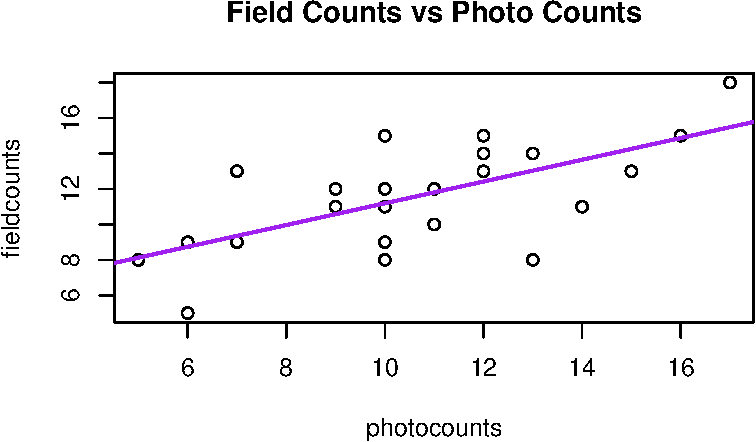
\includegraphics[keepaspectratio]{ratio_files/figure-pdf/fig-deadtrees-regression-fit-1.pdf}}

}

\caption{\label{fig-deadtrees-regression-fit}Field counts vs.~photo
counts of dead trees with the fitted regression line}

\end{figure}%

Let's compare the three different estimation methods to see which
provides the lowest Standard Error for the population mean.

\begin{Shaded}
\begin{Highlighting}[]
\CommentTok{\# 1. Regression estimate for the mean}
\NormalTok{res\_dt\_reg }\OtherTok{\textless{}{-}} \FunctionTok{reg\_est}\NormalTok{(}\AttributeTok{ydata =}\NormalTok{ fieldcounts, }\AttributeTok{xdata =}\NormalTok{ photocounts, }\AttributeTok{xbarU =} \FloatTok{11.3}\NormalTok{, }\AttributeTok{N =} \DecValTok{100}\NormalTok{, }\AttributeTok{estimate =} \StringTok{"mean"}\NormalTok{)}
\NormalTok{res\_dt\_reg}\SpecialCharTok{$}\NormalTok{table}
\end{Highlighting}
\end{Shaded}

\begin{table}[H]
\caption*{
{\large  Regression Estimation: Working Table\normalsize } \\ 
{\normalsize  \(n = 25\)\normalsize }
} 
\normalsize
\begin{gtfit}{\linewidth}{>{\raggedright\arraybackslash}p{\dimexpr 30.00pt -2\tabcolsep-1.5\arrayrulewidth}>{\raggedleft\arraybackslash}p{\dimexpr 75.00pt -2\tabcolsep-1.5\arrayrulewidth}>{\raggedleft\arraybackslash}p{\dimexpr 75.00pt -2\tabcolsep-1.5\arrayrulewidth}>{\raggedleft\arraybackslash}p{\dimexpr 75.00pt -2\tabcolsep-1.5\arrayrulewidth}>{\raggedleft\arraybackslash}p{\dimexpr 75.00pt -2\tabcolsep-1.5\arrayrulewidth}>{\raggedleft\arraybackslash}p{\dimexpr 75.00pt -2\tabcolsep-1.5\arrayrulewidth}}
\toprule
\(i\) & \(y_i\) & \(x_i\) & \(\hat y_i\)\textsuperscript{\textit{1}} & \(e_i\) & \(e_i^2\) \\ 
\midrule\addlinespace[2.5pt]
1 & 15.00 & 10.00 & 11.19 & 3.81 & 14.50 \\ 
2 & 14.00 & 12.00 & 12.42 & 1.58 & 2.50 \\ 
3 & 9.00 & 7.00 & 9.35 & -0.35 & 0.12 \\ 
4 & 14.00 & 13.00 & 13.03 & 0.97 & 0.94 \\ 
5 & 8.00 & 13.00 & 13.03 & -5.03 & 25.32 \\ 
6 & 5.00 & 6.00 & 8.74 & -3.74 & 13.98 \\ 
... & ... & ... & ... & ... & ... \\ 
{\bfseries Sum} & {\bfseries 289.00} & {\bfseries 265.00} & {\bfseries 289.00} & {\bfseries 0.00} & {\bfseries 133.16} \\ 
\bottomrule
\end{gtfit}
\begin{minipage}{\linewidth}
\vspace{.05em}
\textsuperscript{\textit{1}}\(\hat B_0 = 5.06\), \(\hat B_1 = 0.61\), \(\hat y_i = \hat B_0 + \hat B_1 x_i\), \(s_e^2 = 5.79\).\\
\(\bar y_{reg} = \hat B_0+\hat B_1\bar x_U = 5.06 + 0.61 \times 11.30 = 11.99\)\\
\(\mathrm{SE}(\bar y_{reg}) = \sqrt{\left(1-\dfrac{n}{N}\right)\dfrac{s_e^2}{n}} = \sqrt{\left(1-\dfrac{25}{100}\right)\dfrac{5.79}{25}} = 0.42\)\\
\end{minipage}
\end{table}

\begin{Shaded}
\begin{Highlighting}[]
\NormalTok{dt\_reg\_raw }\OtherTok{\textless{}{-}}\NormalTok{ res\_dt\_reg}\SpecialCharTok{$}\NormalTok{estimate}
\NormalTok{dt\_reg\_raw }\SpecialCharTok{|\textgreater{}} \FunctionTok{format\_est\_gt}\NormalTok{(}\StringTok{"reg\_mean"}\NormalTok{)}
\end{Highlighting}
\end{Shaded}

\begin{table}[H]
\normalsize
\begin{gtfit}{0.7\linewidth}{rrrr}
\toprule
\(\bar{y}_{reg}\) & \(\mathrm{SE}(\bar{y}_{reg})\) & 95\% CI Lower & 95\% CI Upper \\ 
\midrule\addlinespace[2.5pt]
11.99 & 0.42 & 11.13 & 12.85 \\ 
\bottomrule
\end{gtfit}
\end{table}

\begin{Shaded}
\begin{Highlighting}[]
\CommentTok{\# (And estimating the total)}
\FunctionTok{reg\_est}\NormalTok{(}\AttributeTok{ydata =}\NormalTok{ fieldcounts, }\AttributeTok{xdata =}\NormalTok{ photocounts, }\AttributeTok{xbarU =} \FloatTok{11.3}\NormalTok{, }\AttributeTok{N =} \DecValTok{100}\NormalTok{, }\AttributeTok{estimate =} \StringTok{"total"}\NormalTok{)}\SpecialCharTok{$}\NormalTok{estimate }\SpecialCharTok{|\textgreater{}}
  \FunctionTok{format\_est\_gt}\NormalTok{(}\StringTok{"reg\_total"}\NormalTok{)}
\end{Highlighting}
\end{Shaded}

\begin{table}[H]
\normalsize
\begin{gtfit}{0.7\linewidth}{rrrr}
\toprule
\(\hat{t}_{reg}\) & \(\mathrm{SE}(\hat{t}_{reg})\) & 95\% CI Lower & 95\% CI Upper \\ 
\midrule\addlinespace[2.5pt]
1,198.93 & 41.68 & 1,112.72 & 1,285.14 \\ 
\bottomrule
\end{gtfit}
\end{table}

\begin{Shaded}
\begin{Highlighting}[]
\CommentTok{\# 2. Simple random sampling estimate for the mean (Ignoring photo counts)}
\NormalTok{res\_dt\_srs }\OtherTok{\textless{}{-}} \FunctionTok{srs\_est}\NormalTok{(}\AttributeTok{sdata =}\NormalTok{ fieldcounts, }\AttributeTok{N =} \DecValTok{100}\NormalTok{, }\AttributeTok{estimate =} \StringTok{"mean"}\NormalTok{, }\AttributeTok{show.details =} \ConstantTok{FALSE}\NormalTok{)}
\NormalTok{dt\_srs\_raw }\OtherTok{\textless{}{-}}\NormalTok{ res\_dt\_srs}\SpecialCharTok{$}\NormalTok{estimate}
\NormalTok{dt\_srs\_raw }\SpecialCharTok{|\textgreater{}} \FunctionTok{format\_est\_gt}\NormalTok{(}\StringTok{"mean"}\NormalTok{)}
\end{Highlighting}
\end{Shaded}

\begin{table}[H]
\normalsize
\begin{gtfit}{0.7\linewidth}{rrrr}
\toprule
\(\bar{y}\) & \(\mathrm{SE}(\bar{y})\) & 95\% CI Lower & 95\% CI Upper \\ 
\midrule\addlinespace[2.5pt]
11.56 & 0.52 & 10.48 & 12.64 \\ 
\bottomrule
\end{gtfit}
\end{table}

\begin{Shaded}
\begin{Highlighting}[]
\CommentTok{\# 3. Ratio estimate for the mean}
\NormalTok{res\_dt\_ratio }\OtherTok{\textless{}{-}} \FunctionTok{ratio\_est}\NormalTok{(}\AttributeTok{ydata =}\NormalTok{ fieldcounts, }\AttributeTok{xdata =}\NormalTok{ photocounts, }\AttributeTok{xbarU =} \FloatTok{11.3}\NormalTok{, }\AttributeTok{N =} \DecValTok{100}\NormalTok{, }\AttributeTok{estimate =} \StringTok{"mean"}\NormalTok{)}
\NormalTok{res\_dt\_ratio}\SpecialCharTok{$}\NormalTok{table}
\end{Highlighting}
\end{Shaded}

\begin{table}[H]
\caption*{
{\large  Ratio Estimation: Working Table\normalsize } \\ 
{\normalsize  \(n = 25\)\normalsize }
} 
\normalsize
\begin{gtfit}{\linewidth}{>{\raggedright\arraybackslash}p{\dimexpr 30.00pt -2\tabcolsep-1.5\arrayrulewidth}>{\raggedleft\arraybackslash}p{\dimexpr 75.00pt -2\tabcolsep-1.5\arrayrulewidth}>{\raggedleft\arraybackslash}p{\dimexpr 75.00pt -2\tabcolsep-1.5\arrayrulewidth}>{\raggedleft\arraybackslash}p{\dimexpr 75.00pt -2\tabcolsep-1.5\arrayrulewidth}>{\raggedleft\arraybackslash}p{\dimexpr 75.00pt -2\tabcolsep-1.5\arrayrulewidth}>{\raggedleft\arraybackslash}p{\dimexpr 75.00pt -2\tabcolsep-1.5\arrayrulewidth}}
\toprule
\(i\) & \(y_i\) & \(x_i\) & \(\hat y_i\)\textsuperscript{\textit{1}} & \(e_i\) & \(e_i^2\) \\ 
\midrule\addlinespace[2.5pt]
1 & 15.00 & 10.00 & 10.91 & 4.09 & 16.76 \\ 
2 & 14.00 & 12.00 & 13.09 & 0.91 & 0.83 \\ 
3 & 9.00 & 7.00 & 7.63 & 1.37 & 1.87 \\ 
4 & 14.00 & 13.00 & 14.18 & -0.18 & 0.03 \\ 
5 & 8.00 & 13.00 & 14.18 & -6.18 & 38.16 \\ 
6 & 5.00 & 6.00 & 6.54 & -1.54 & 2.38 \\ 
... & ... & ... & ... & ... & ... \\ 
{\bfseries Sum} & {\bfseries 289.00} & {\bfseries 265.00} & {\bfseries 289.00} & {\bfseries 0.00} & {\bfseries 184.64} \\ 
\bottomrule
\end{gtfit}
\begin{minipage}{\linewidth}
\vspace{.05em}
\textsuperscript{\textit{1}}\(\hat B = \sum_i y_i / \sum_i x_i = 1.09\), \(\hat y_i = \hat B\, x_i\), \(s_e^2 = 7.69\).\\
\(\bar y_r = \hat B\,\bar x_U = 1.09 \times 11.30 = 12.32\)\\
\(\mathrm{SE}(\bar y_r) = \mathrm{SE}(\hat B)\,\bar x_U = 0.05 \times 11.30 = 0.51\)\\
\end{minipage}
\end{table}

\begin{Shaded}
\begin{Highlighting}[]
\NormalTok{dt\_ratio\_raw }\OtherTok{\textless{}{-}}\NormalTok{ res\_dt\_ratio}\SpecialCharTok{$}\NormalTok{estimate}
\NormalTok{dt\_ratio\_raw }\SpecialCharTok{|\textgreater{}} \FunctionTok{format\_est\_gt}\NormalTok{(}\StringTok{"ratio\_mean"}\NormalTok{)}
\end{Highlighting}
\end{Shaded}

\begin{table}[H]
\normalsize
\begin{gtfit}{0.7\linewidth}{rrrr}
\toprule
\(\bar{y}_{r}\) & \(\mathrm{SE}(\bar{y}_{r})\) & 95\% CI Lower & 95\% CI Upper \\ 
\midrule\addlinespace[2.5pt]
12.32 & 0.51 & 11.27 & 13.38 \\ 
\bottomrule
\end{gtfit}
\end{table}

\paragraph*{Output Note:}\label{output-note}
\addcontentsline{toc}{paragraph}{Output Note:}

\begin{itemize}
\item
  \textbf{SRS Mean:} SE = 0.522
\item
  \textbf{Ratio Mean:} SE = 0.512
\item
  \textbf{Regression Mean:} SE = 0.417
\end{itemize}

The sampled plots average \(\bar x = 10.6\) photo-counted trees, below
the population average \(\bar x_U = 11.3\), so both the ratio and the
regression estimates are above the plain sample mean \(\bar y = 11.56\).
The ratio estimator barely improves on SRS, since a line through the
origin fits these data poorly. Because the intercept of the true line is
non-zero, the \textbf{regression estimator} provides the most precise
estimate in this scenario.

\subsection{Shinylive App Illustrating Ratio Estimation and Regression
Estimation}\label{shinylive-app-illustrating-ratio-estimation-and-regression-estimation}

The simulation for this section runs as a standalone app:
\href{../shinylives_sampling/app-ratio.html}{Ratio Estimation and
Regression Estimation}. It opens in a new tab, together with its
documentation and the full \href{../shinylives_sampling/index.html}{list
of apps}.

\section{Post-stratification}\label{post-stratification}

\subsection{Theory}\label{sec-poststrat-theory}

\subsubsection{The post-stratified
estimator}\label{the-post-stratified-estimator}

Sometimes a unit's stratum is unknown until \emph{after} sampling, for
instance a person's gender before the interview. We cannot then stratify
in advance, but if the true population sizes \(N_h\) of the \(H\) groups
are known from another source, we can still take an SRS, sort the units
into groups afterwards, and weight each group mean by its \emph{known}
population share \(\pi_h = N_h/N\), as in stratified sampling: \[
\boxed{\bar y_{post} = \sum_{h=1}^H \pi_h\,\bar y_h,
\qquad
\hat t_{post} = N\bar y_{post}}.
\] Compare this with the unweighted mean
\(\bar y = \sum_h (n_h/n)\,\bar y_h\), which weights the groups by the
shares the sample happened to deliver. When the sample over- or
under-represents a group, post-stratification corrects for it.

It also has a predictive reading, like the ratio and regression
estimators. Every unit in group \(h\) is predicted by that group's
sample mean, \(\hat y_i = \bar y_h\) for \(i \in \mathcal U_h\), so \[
\hat t_{post} = \sum_{i \in \mathcal U}\hat y_i = \sum_{h=1}^H N_h\,\bar y_h,
\qquad
\hat{\bar y}_{post} = \sum_{h=1}^H \pi_h\,\bar y_h .
\]

Figure~\ref{fig-poststrat-concept} illustrates the benefit. The grey
points are the population, split into post-strata A to D (the width of
each block is \(N_h\)). The green circles are an ordinary SRS of
\(n = 25\); the realized \(n_h = (5, 5, 6, 9)\) do \emph{not} match the
population shares \(\pi_h = (.36, .14, .21, .29)\), and they never do,
since \(n_h\) is random. The red segments are the predictions
\(\hat y_i = \bar y_h\) in each stratum, whose weighted average is
\(\hat{\bar y}_{post}\).

\begin{Shaded}
\begin{Highlighting}[]
\FunctionTok{plot\_poststrat\_concept}\NormalTok{()}
\end{Highlighting}
\end{Shaded}

\begin{figure}[H]

\centering{

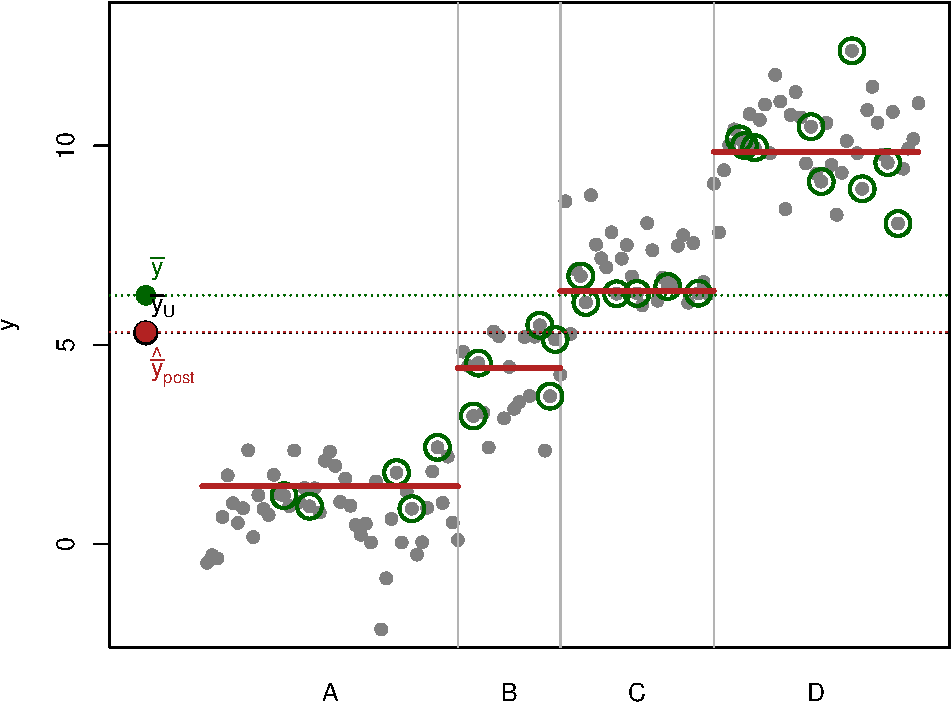
\includegraphics[width=0.7\linewidth,height=\textheight,keepaspectratio]{ratio_files/figure-pdf/fig-poststrat-concept-1.pdf}

}

\caption{\label{fig-poststrat-concept}Illustration of the benefits of
post-stratification.}

\end{figure}%

This sample is light on A and heavy on D, so the naive \(\bar y\)
(green) is pulled up; reweighting by the known \(\pi_h\) undoes it, and
\(\hat{\bar y}_{post}\) (red) is close to \(\bar y_U\) (black). It is
this reweighting, repeated over samples, that cuts the variance.

\subsubsection{Variance of the post-stratified
mean}\label{variance-of-the-post-stratified-mean}

The observed group sizes \(n_h\) are random, so for the variance we
substitute their expected values under SRS, the proportional sample
sizes \[
n_h^{post} = n\,\frac{N_h}{N} = n\pi_h ,
\] into the stratified variance formula. Every group then has sampling
fraction \(n_h^{post}/N_h = n/N\), so the finite population correction
is the same in all groups and the variance simplifies: \[
\boxed{\hat V(\bar y_{post}) = \sum_{h=1}^H \pi_h^2\left(1 - \frac{n_h^{post}}{N_h}\right)\frac{s_h^2}{n_h^{post}}
= \left(1 - \frac nN\right)\frac1n\sum_{h=1}^H \pi_h s_h^2},
\] the variance of proportional stratified sampling: the SRS variance
with \(s^2\) replaced by the weighted average of the within-group
variances. Also \(\hat V(\hat t_{post}) = N^2\hat V(\bar y_{post})\).
Here \(n_h\), \(\bar y_h\) and \(s_h^2\) are the count, mean and
variance of the units the sample happened to place in group \(h\), so
every group needs \(n_h \geq 2\) for \(s_h^2\) to exist. Substituting
\(n_h^{post}\) treats the \(n_h\) as fixed at \(n\pi_h\); carrying their
randomness adds a second-order term
\(\frac{1}{n^2}\sum_h(1 - \pi_h)s_h^2\), negligible unless some \(n_h\)
are small.

\subsubsection{Post-stratification as a regression
estimator}\label{sec-poststrat-regression}

Post-stratification is not a separate technique: it is the regression
estimator of Section~\ref{sec-regression-theory} with the \textbf{group
indicators} as the auxiliary variables. Take the \(H\) dummies
\(x_{ih} = \mathbf 1\{i \in \text{group } h\}\) and fit without an
intercept. Then

\begin{itemize}
\tightlist
\item
  the fitted coefficients are the group means, \(\hat B_h = \bar y_h\);
\item
  the population means of those dummies are the known weights,
  \(\bar x_{U,h} = N_h/N = \pi_h\);
\end{itemize}

so the regression estimator \emph{is} the post-stratified one, \[
\hat{\bar y}_{reg} = \sum_h \hat B_h\,\bar x_{U,h} = \sum_h \pi_h\bar y_h = \hat{\bar y}_{post} .
\] Its residuals are each unit's deviation from its own group mean,
\(e_i = y_i - \bar y_{h(i)}\), and the regression variance
\(\left(1 - \frac nN\right)s_e^2/n\) applies with \(p = H\) fitted
parameters: \[
s_e^2 = \frac{1}{n-H}\sum_h\sum_{i \in h}\left(y_i - \bar y_h\right)^2 = \sum_h \frac{n_h - 1}{n-H}\,s_h^2 .
\] Dropping the \(-1\) and the \(-H\) (small relative to \(n_h\) and
\(n\)), and then using \(n_h/n \approx \pi_h\), the regression variance
reduces to the post-stratified one: \[
\begin{aligned}
\hat V(\hat{\bar y}_{reg})
&= \left(1 - \frac nN\right)\frac1n\sum_{h=1}^H \frac{n_h - 1}{n-H}\,s_h^2 \\
&\approx \left(1 - \frac nN\right)\frac1n\sum_{h=1}^H \frac{n_h}{n}\,s_h^2 \\
&\approx \left(1 - \frac nN\right)\frac1n\sum_{h=1}^H \pi_h\,s_h^2
= \hat V(\hat{\bar y}_{post}) .
\end{aligned}
\] Both are weighted averages of the \emph{same} \(s_h^2\); only the
weights differ, \[
\underbrace{\frac{n_h - 1}{n - H}}_{\text{sample proportions}}
\qquad\text{versus}\qquad
\underbrace{\pi_h = \frac{N_h}{N}}_{\text{population proportions}} .
\] So the substitution \(n_h \to n\pi_h\) above is simply: \emph{pool
the residuals with the weights we know, not with the ones the sample
happened to deliver.} It is the same reasoning that puts \(\bar x_U\),
rather than \(\bar x\), in the ratio estimator.

Seen this way, the estimators of this chapter are one estimator with
different auxiliary variables, and \(s_e^2 = \frac{1}{n-p}\sum_i e_i^2\)
throughout, where \(p\) is the number of fitted parameters:

{\def\LTcaptype{none} % do not increment counter
\begin{longtable}[]{@{}
  >{\raggedright\arraybackslash}p{(\linewidth - 6\tabcolsep) * \real{0.2500}}
  >{\raggedright\arraybackslash}p{(\linewidth - 6\tabcolsep) * \real{0.2500}}
  >{\raggedright\arraybackslash}p{(\linewidth - 6\tabcolsep) * \real{0.2500}}
  >{\centering\arraybackslash}p{(\linewidth - 6\tabcolsep) * \real{0.2500}}@{}}
\toprule\noalign{}
\begin{minipage}[b]{\linewidth}\raggedright
Estimator
\end{minipage} & \begin{minipage}[b]{\linewidth}\raggedright
Auxiliary variables
\end{minipage} & \begin{minipage}[b]{\linewidth}\raggedright
Residual \(e_i\)
\end{minipage} & \begin{minipage}[b]{\linewidth}\centering
\(p\)
\end{minipage} \\
\midrule\noalign{}
\endhead
\bottomrule\noalign{}
\endlastfoot
Ratio & one \(x\), line forced through the origin & \(y_i - \hat B x_i\)
& 1 \\
Regression & intercept and \(x\) & \(y_i - \hat B_0 - \hat B_1 x_i\) &
2 \\
Post-stratification & \(H\) group indicators & \(y_i - \bar y_h\) &
\(H\) \\
\end{longtable}
}

Domain estimation, treated next, stands slightly apart: there the
divisor is the random \(n_d\) rather than the full \(n\), because only
the units falling in the domain carry information about it.

\subsection{Example: A Nurses Survey (by
hand)}\label{example-a-nurses-survey-by-hand}

A survey of \(N = 10{,}000\) people, half women and half men, takes an
SRS of \(n = 400\) and asks whether they want to become a nurse. The
sample has three times as many women as men, though the population is
50/50:

{\def\LTcaptype{none} % do not increment counter
\begin{longtable}[]{@{}lrrrr@{}}
\toprule\noalign{}
Stratum & \(N_h\) & \(n_h\) & Want nurse & \(\hat p_h\) \\
\midrule\noalign{}
\endhead
\bottomrule\noalign{}
\endlastfoot
Female & 5000 & 300 & 150 & 0.50 \\
Male & 5000 & 100 & 10 & 0.10 \\
\end{longtable}
}

Ignoring this pulls the estimate
\(\hat p_{SRS} = \frac{160}{400} = (0.5)(0.75) + (0.1)(0.25) = 0.4\)
toward the female (higher) rate. Weighting by the \emph{known}
population shares instead gives \[
\hat p_{post} = \hat p_f\frac{N_f}{N} + \hat p_m\frac{N_m}{N} = (0.5)(0.5) + (0.1)(0.5) = 0.3 .
\]

For the standard error, \(\hat p_h\) plays the role of \(\bar y_h\), and
\(s_h^2 = \frac{n_h}{n_h-1}\hat p_h(1 - \hat p_h)\) from the realized
counts. With the working sample sizes \(n_h^{post} = n\pi_h = 200\) in
each stratum (proportional to size allocation), every finite population
correction is \(1 - n/N = 0.96\):

{\def\LTcaptype{none} % do not increment counter
\begin{longtable}[]{@{}
  >{\raggedright\arraybackslash}p{(\linewidth - 14\tabcolsep) * \real{0.1250}}
  >{\raggedleft\arraybackslash}p{(\linewidth - 14\tabcolsep) * \real{0.1250}}
  >{\raggedleft\arraybackslash}p{(\linewidth - 14\tabcolsep) * \real{0.1250}}
  >{\raggedleft\arraybackslash}p{(\linewidth - 14\tabcolsep) * \real{0.1250}}
  >{\raggedleft\arraybackslash}p{(\linewidth - 14\tabcolsep) * \real{0.1250}}
  >{\raggedleft\arraybackslash}p{(\linewidth - 14\tabcolsep) * \real{0.1250}}
  >{\raggedleft\arraybackslash}p{(\linewidth - 14\tabcolsep) * \real{0.1250}}
  >{\raggedleft\arraybackslash}p{(\linewidth - 14\tabcolsep) * \real{0.1250}}@{}}
\toprule\noalign{}
\begin{minipage}[b]{\linewidth}\raggedright
Post-stratum
\end{minipage} & \begin{minipage}[b]{\linewidth}\raggedleft
\(N_h\)
\end{minipage} & \begin{minipage}[b]{\linewidth}\raggedleft
\(\pi_h\)
\end{minipage} & \begin{minipage}[b]{\linewidth}\raggedleft
\(n_h^{post}\)
\end{minipage} & \begin{minipage}[b]{\linewidth}\raggedleft
\(\hat p_h\)
\end{minipage} & \begin{minipage}[b]{\linewidth}\raggedleft
\(s_h^2\)
\end{minipage} & \begin{minipage}[b]{\linewidth}\raggedleft
\(\pi_h\hat p_h\)
\end{minipage} & \begin{minipage}[b]{\linewidth}\raggedleft
\(\hat v_h\)
\end{minipage} \\
\midrule\noalign{}
\endhead
\bottomrule\noalign{}
\endlastfoot
Female & 5000 & 0.5 & 200 & 0.500 & 0.2508 & 0.2500 & 0.000301 \\
Male & 5000 & 0.5 & 200 & 0.100 & 0.0909 & 0.0500 & 0.000109 \\
\textbf{Total} & \textbf{10000} & \textbf{1.0} & \textbf{400} & & &
\textbf{0.3000} & \textbf{0.000410} \\
\end{longtable}
}

where
\(\hat v_h = \left(1 - n_h^{post}/N_h\right)\pi_h^2\,s_h^2/n_h^{post}\).
The short-cut formula gives the same variance without the working sample
sizes, using \(\sum_h\pi_hs_h^2 = 0.5(0.2508) + 0.5(0.0909) = 0.1709\):
\[
\hat V(\hat p_{post}) = \left(1 - \frac nN\right)\frac1n\sum_h\pi_hs_h^2 = \frac{0.96}{400}(0.1709) = 0.000410 .
\] So \(\text{SE}(\hat p_{post}) = \sqrt{0.000410} = 0.0203\) and an
approximate 95\% interval is
\(0.300 \pm 1.96(0.0203) = [0.260,\ 0.340]\). Treating the data as an
unstratified SRS gives \(\hat p_{SRS} = 0.4\) with
\(\text{SE} = \sqrt{\left(1 - \frac{400}{10000}\right)\frac{(0.4)(0.6)}{399}} \approx 0.0240\).
Post-stratification is both unbiased and more precise, since it removes
the between-sex variability from the standard error.

\subsection{Example: agsrs\_syn.csv}\label{example-agsrs_syn.csv}

Any variable known for \textbf{every} unit of the population can be used
to post-stratify an SRS. We use \texttt{agsrs\_syn.csv}, a simple random
sample of \(n=300\) counties drawn without replacement from the
population in \texttt{agpop.csv} (the script
\texttt{data/make\_agsrs\_syn.R} shows how), and compare two
post-stratifiers: the census \textbf{region}, and \textbf{quantile
groups of \texttt{acres87}} (the 1987 acreage, as in the
post-stratification app). The population is the \(N=3041\) counties with
no missing value in \texttt{acres92}, \texttt{acres87}, \texttt{acres82}
or \texttt{farms92}.

\subsubsection{By Region}\label{by-region}

If we know the true regional population sizes (\(N_h\)), we can
post-stratify our SRS data.

The population is read from \texttt{agpop.csv}, keeping the counties
with no missing value, and the sample from \texttt{agsrs\_syn.csv};
acreages are converted to thousands of acres.

\begin{Shaded}
\begin{Highlighting}[]
\DocumentationTok{\#\# the population, and the sample drawn from it (acres in thousands)}
\NormalTok{agpop\_ps }\OtherTok{\textless{}{-}} \FunctionTok{acres\_in\_thousands}\NormalTok{(}\FunctionTok{read.csv}\NormalTok{(}\StringTok{"data/agpop.csv"}\NormalTok{))}
\NormalTok{agpop\_ps }\OtherTok{\textless{}{-}}\NormalTok{ agpop\_ps[}\FunctionTok{complete.cases}\NormalTok{(agpop\_ps[, }\FunctionTok{c}\NormalTok{(}\StringTok{"acres92"}\NormalTok{, }\StringTok{"acres87"}\NormalTok{, }\StringTok{"acres82"}\NormalTok{, }\StringTok{"farms92"}\NormalTok{)]), ]}
\NormalTok{N }\OtherTok{\textless{}{-}} \FunctionTok{nrow}\NormalTok{(agpop\_ps)}
\NormalTok{agsrs\_syn }\OtherTok{\textless{}{-}} \FunctionTok{acres\_in\_thousands}\NormalTok{(}\FunctionTok{read.csv}\NormalTok{(}\StringTok{"data/agsrs\_syn.csv"}\NormalTok{))}
\end{Highlighting}
\end{Shaded}

From the sample we need the observed group sizes \(n_h\), the group
means \(\bar y_h\) and the group standard deviations \(s_h\). The
regional population sizes \(N_h\) are the external information, taken
from the population.

\begin{Shaded}
\begin{Highlighting}[]
\NormalTok{nh }\OtherTok{\textless{}{-}} \FunctionTok{tapply}\NormalTok{(agsrs\_syn[, }\StringTok{"acres92"}\NormalTok{], agsrs\_syn[,}\StringTok{"region"}\NormalTok{], length)}
\NormalTok{n }\OtherTok{\textless{}{-}} \FunctionTok{sum}\NormalTok{(nh)}
\NormalTok{sh }\OtherTok{\textless{}{-}} \FunctionTok{tapply}\NormalTok{(agsrs\_syn[, }\StringTok{"acres92"}\NormalTok{], agsrs\_syn[,}\StringTok{"region"}\NormalTok{], sd)}
\NormalTok{ybarh }\OtherTok{\textless{}{-}} \FunctionTok{tapply}\NormalTok{(agsrs\_syn[, }\StringTok{"acres92"}\NormalTok{], agsrs\_syn[,}\StringTok{"region"}\NormalTok{], mean)}
\CommentTok{\# external information: the regional population sizes}
\NormalTok{Nh }\OtherTok{\textless{}{-}} \FunctionTok{tapply}\NormalTok{(agpop\_ps}\SpecialCharTok{$}\NormalTok{acres92, agpop\_ps}\SpecialCharTok{$}\NormalTok{region, length)}
\end{Highlighting}
\end{Shaded}

\textbf{Create \(n_h^{\text{post-strat}} = n \times \frac{N_h}{N}\)},
instead of using the randomly observed \(n_h\).

\begin{Shaded}
\begin{Highlighting}[]
\NormalTok{nh\_post }\OtherTok{\textless{}{-}}\NormalTok{ Nh }\SpecialCharTok{/} \FunctionTok{sum}\NormalTok{(Nh) }\SpecialCharTok{*}\NormalTok{ n}

\DocumentationTok{\#\# regional summary for stratified sampling estimation}
\FunctionTok{data.frame}\NormalTok{(}
  \AttributeTok{ybarh =}\NormalTok{ ybarh, }
  \AttributeTok{sh =}\NormalTok{ sh, }
  \AttributeTok{nh =}\NormalTok{ nh, }
  \AttributeTok{pi\_obs =}\NormalTok{ nh}\SpecialCharTok{/}\NormalTok{n, }
  \AttributeTok{Nh =}\NormalTok{ Nh, }
  \AttributeTok{pi\_pop =}\NormalTok{ Nh}\SpecialCharTok{/}\FunctionTok{sum}\NormalTok{(Nh),  }
  \AttributeTok{nh\_post =}\NormalTok{ nh\_post}
\NormalTok{) }\SpecialCharTok{|\textgreater{}} 
  \FunctionTok{gt}\NormalTok{(}\AttributeTok{rownames\_to\_stub =} \ConstantTok{TRUE}\NormalTok{) }\SpecialCharTok{|\textgreater{}}
  \FunctionTok{cols\_label}\NormalTok{(}
    \AttributeTok{ybarh =} \FunctionTok{md}\NormalTok{(}\StringTok{"$}\SpecialCharTok{\textbackslash{}\textbackslash{}}\StringTok{bar\{y\}\_h$"}\NormalTok{),}
    \AttributeTok{sh =} \FunctionTok{md}\NormalTok{(}\StringTok{"$s\_h$"}\NormalTok{),}
    \AttributeTok{nh =} \FunctionTok{md}\NormalTok{(}\StringTok{"$n\_h\^{}\{}\SpecialCharTok{\textbackslash{}\textbackslash{}}\StringTok{text\{obs\}\}$"}\NormalTok{),}
    \AttributeTok{pi\_obs =} \FunctionTok{md}\NormalTok{(}\StringTok{"$}\SpecialCharTok{\textbackslash{}\textbackslash{}}\StringTok{pi\^{}\{}\SpecialCharTok{\textbackslash{}\textbackslash{}}\StringTok{text\{obs\}\}\_h$"}\NormalTok{),}
    \AttributeTok{Nh =} \FunctionTok{md}\NormalTok{(}\StringTok{"$N\_h$"}\NormalTok{),}
    \AttributeTok{pi\_pop =} \FunctionTok{md}\NormalTok{(}\StringTok{"$}\SpecialCharTok{\textbackslash{}\textbackslash{}}\StringTok{pi\^{}\{}\SpecialCharTok{\textbackslash{}\textbackslash{}}\StringTok{text\{pop\}\}\_h$"}\NormalTok{),}
    \AttributeTok{nh\_post =} \FunctionTok{md}\NormalTok{(}\StringTok{"$n\_h\^{}\{}\SpecialCharTok{\textbackslash{}\textbackslash{}}\StringTok{text\{post\}\}$"}\NormalTok{)}
\NormalTok{  ) }\SpecialCharTok{|\textgreater{}} 
  \FunctionTok{fmt\_number}\NormalTok{(}\AttributeTok{columns =} \FunctionTok{c}\NormalTok{(ybarh, sh, pi\_obs, pi\_pop, nh\_post), }\AttributeTok{decimals =} \DecValTok{3}\NormalTok{)}
\end{Highlighting}
\end{Shaded}

\begin{table}

\caption{\label{tbl-agsrs-poststrat-summary}Observed vs.~population
stratum proportions and post-stratified sample sizes}

\centering{

\normalsize
\begin{gtfit}{\linewidth}{l|rrrrrrr}
\toprule
 & \(\bar{y}_h\) & \(s_h\) & \(n_h^{\text{obs}}\) & \(\pi^{\text{obs}}_h\) & \(N_h\) & \(\pi^{\text{pop}}_h\) & \(n_h^{\text{post}}\) \\ 
\midrule\addlinespace[2.5pt]
NC & 355.048 & 260.114 & 110 & 0.367 & 1049 & 0.345 & 103.486 \\ 
NE & 62.613 & 61.156 & 17 & 0.057 & 211 & 0.069 & 20.816 \\ 
S & 201.874 & 197.338 & 126 & 0.420 & 1368 & 0.450 & 134.956 \\ 
W & 613.793 & 691.154 & 47 & 0.157 & 413 & 0.136 & 40.743 \\ 
\bottomrule
\end{gtfit}

}

\end{table}%

\textbf{Output Note:} The table above shows the difference between the
sample proportion (\(\pi^{obs}_h\)) and the true population proportion
(\(\pi^{pop}_h\)). Post-stratification forces the weights to reflect the
true population structure.

The post-stratified estimate comes from \texttt{str\_est()}, applied
with the working sample sizes \(n_h^{\text{post}}\). For comparison we
also compute the unadjusted SRS estimate, and the true mean of the
population.

\begin{Shaded}
\begin{Highlighting}[]
\DocumentationTok{\#\# strata mean estimate}
\NormalTok{res\_post\_strat }\OtherTok{\textless{}{-}} \FunctionTok{str\_est}\NormalTok{(ybarh, sh, nh\_post, Nh, }\AttributeTok{estimate =} \StringTok{"mean"}\NormalTok{)}
\NormalTok{res\_post\_strat}\SpecialCharTok{$}\NormalTok{table}
\end{Highlighting}
\end{Shaded}

\begin{table}[H]
\caption*{
{\large  Stratified Mean Estimation: Working Table\normalsize }
} 
\normalsize
\begin{gtfit}{\linewidth}{>{\raggedright\arraybackslash}p{\dimexpr 82.50pt -2\tabcolsep-1.5\arrayrulewidth}>{\raggedleft\arraybackslash}p{\dimexpr 45.00pt -2\tabcolsep-1.5\arrayrulewidth}>{\raggedleft\arraybackslash}p{\dimexpr 45.00pt -2\tabcolsep-1.5\arrayrulewidth}>{\raggedleft\arraybackslash}p{\dimexpr 82.50pt -2\tabcolsep-1.5\arrayrulewidth}>{\raggedleft\arraybackslash}p{\dimexpr 82.50pt -2\tabcolsep-1.5\arrayrulewidth}>{\raggedleft\arraybackslash}p{\dimexpr 82.50pt -2\tabcolsep-1.5\arrayrulewidth}>{\raggedleft\arraybackslash}p{\dimexpr 82.50pt -2\tabcolsep-1.5\arrayrulewidth}>{\raggedleft\arraybackslash}p{\dimexpr 82.50pt -2\tabcolsep-1.5\arrayrulewidth}}
\toprule
Stratum & \(N_h\) & \(n_h\) & \(\pi_h\)\textsuperscript{\textit{1}} & \(\bar y_h\) & \(s_h^2\) & \(\pi_h\bar y_h\) & \(v_h\)\textsuperscript{\textit{2}} \\ 
\midrule\addlinespace[2.5pt]
NC & 1,049 & 103 & 0.34 & 355.05 & 67,659.15 & 122.47 & 70.12 \\ 
NE & 211 & 21 & 0.07 & 62.61 & 3,740.00 & 4.34 & 0.78 \\ 
S & 1,368 & 135 & 0.45 & 201.87 & 38,942.48 & 90.81 & 52.63 \\ 
W & 413 & 41 & 0.14 & 613.79 & 477,694.47 & 83.36 & 194.92 \\ 
{\bfseries Total} & {\bfseries 3,041} & {\bfseries 300} & {\bfseries 1.00} & {\bfseries } & {\bfseries } & {\bfseries 300.99} & {\bfseries 318.46} \\ 
\bottomrule
\end{gtfit}
\begin{minipage}{\linewidth}
\vspace{.05em}
\textsuperscript{\textit{1}}\(\pi_h = N_h/N\) is the stratum weight.\\
\textsuperscript{\textit{2}}\(v_h = (1-n_h/N_h)\,\pi_h^2\, s_h^2/n_h\) is stratum \(h\)'s contribution to \(V(\bar y_{str}) = \sum_h v_h\).\\
\(\bar y_{str} = \sum_h \pi_h\bar y_h = 300.99\)\\
\(\mathrm{SE}(\bar y_{str}) = \sqrt{\sum_h v_h} = \sqrt{318.46} = 17.85\)\\
\end{minipage}
\end{table}

\begin{Shaded}
\begin{Highlighting}[]
\NormalTok{post\_strat\_est }\OtherTok{\textless{}{-}}\NormalTok{ res\_post\_strat}\SpecialCharTok{$}\NormalTok{estimate}
\NormalTok{post\_strat\_est }\SpecialCharTok{|\textgreater{}} \FunctionTok{format\_est\_gt}\NormalTok{(}\StringTok{"mean"}\NormalTok{)}
\end{Highlighting}
\end{Shaded}

\begin{table}[H]
\normalsize
\begin{gtfit}{0.7\linewidth}{rrrr}
\toprule
\(\bar{y}\) & \(\mathrm{SE}(\bar{y})\) & 95\% CI Lower & 95\% CI Upper \\ 
\midrule\addlinespace[2.5pt]
300.99 & 17.85 & 266.02 & 335.97 \\ 
\bottomrule
\end{gtfit}
\end{table}

\begin{Shaded}
\begin{Highlighting}[]
\DocumentationTok{\#\# compare with SRS estimate}
\NormalTok{res\_srs\_est }\OtherTok{\textless{}{-}} \FunctionTok{srs\_est}\NormalTok{(agsrs\_syn}\SpecialCharTok{$}\NormalTok{acres92, }\AttributeTok{N =}\NormalTok{ N, }\AttributeTok{estimate =} \StringTok{"mean"}\NormalTok{, }\AttributeTok{show.details =} \ConstantTok{FALSE}\NormalTok{)}
\NormalTok{srs\_est\_raw }\OtherTok{\textless{}{-}}\NormalTok{ res\_srs\_est}\SpecialCharTok{$}\NormalTok{estimate}
\NormalTok{srs\_est\_raw }\SpecialCharTok{|\textgreater{}} \FunctionTok{format\_est\_gt}\NormalTok{(}\StringTok{"mean"}\NormalTok{)}
\end{Highlighting}
\end{Shaded}

\begin{table}[H]
\normalsize
\begin{gtfit}{0.7\linewidth}{rrrr}
\toprule
\(\bar{y}\) & \(\mathrm{SE}(\bar{y})\) & 95\% CI Lower & 95\% CI Upper \\ 
\midrule\addlinespace[2.5pt]
314.68 & 20.38 & 274.57 & 354.79 \\ 
\bottomrule
\end{gtfit}
\end{table}

\begin{Shaded}
\begin{Highlighting}[]
\DocumentationTok{\#\# true mean check}
\FunctionTok{mean}\NormalTok{(agpop\_ps}\SpecialCharTok{$}\NormalTok{acres92)}
\end{Highlighting}
\end{Shaded}

\begin{verbatim}
[1] 309.9421
\end{verbatim}

\textbf{Output Note:} The post-stratified estimate gives a Standard
Error of 17.8, which is more precise than the unadjusted SRS standard
error of 20.4.

The same standard error follows from the short-cut formula
\(\hat V = \left(1-\frac nN\right)\frac1n\sum_h\pi_h s_h^2\) of
Section~\ref{sec-poststrat-theory}, which needs only the population
shares \(\pi_h\) and the group variances, not the working sample sizes.
The working table lists \(\bar y_h\), \(s_h^2\) and \(\pi_h\), and the
two working columns \(\pi_h\bar y_h\) and \(\pi_h s_h^2\), whose totals
are \(\bar y_{post}\) and \(\sum_h\pi_hs_h^2\):

\begin{Shaded}
\begin{Highlighting}[]
\DocumentationTok{\#\# working table for the short{-}cut formula, given the group sizes and the group means and sds}
\NormalTok{shortcut\_table }\OtherTok{\textless{}{-}} \ControlFlowTok{function}\NormalTok{(Nh, ybarh, sh) \{}
\NormalTok{  work }\OtherTok{\textless{}{-}} \FunctionTok{data.frame}\NormalTok{(}\AttributeTok{Nh =} \FunctionTok{as.vector}\NormalTok{(Nh), }\AttributeTok{pi\_h =} \FunctionTok{as.vector}\NormalTok{(Nh) }\SpecialCharTok{/} \FunctionTok{sum}\NormalTok{(Nh),}
                     \AttributeTok{ybarh =} \FunctionTok{as.vector}\NormalTok{(ybarh), }\AttributeTok{s2h =} \FunctionTok{as.vector}\NormalTok{(sh)}\SpecialCharTok{\^{}}\DecValTok{2}\NormalTok{,}
                     \AttributeTok{row.names =} \FunctionTok{names}\NormalTok{(Nh))}
\NormalTok{  work}\SpecialCharTok{$}\NormalTok{pi\_ybar }\OtherTok{\textless{}{-}}\NormalTok{ work}\SpecialCharTok{$}\NormalTok{pi\_h }\SpecialCharTok{*}\NormalTok{ work}\SpecialCharTok{$}\NormalTok{ybarh      }\CommentTok{\# working column: pi\_h * ybar\_h}
\NormalTok{  work}\SpecialCharTok{$}\NormalTok{pi\_s2   }\OtherTok{\textless{}{-}}\NormalTok{ work}\SpecialCharTok{$}\NormalTok{pi\_h }\SpecialCharTok{*}\NormalTok{ work}\SpecialCharTok{$}\NormalTok{s2h        }\CommentTok{\# working column: pi\_h * s\_h\^{}2}
  \FunctionTok{rbind}\NormalTok{(work, }\AttributeTok{Total =} \FunctionTok{c}\NormalTok{(}\FunctionTok{sum}\NormalTok{(work}\SpecialCharTok{$}\NormalTok{Nh), }\FunctionTok{sum}\NormalTok{(work}\SpecialCharTok{$}\NormalTok{pi\_h), }\ConstantTok{NA}\NormalTok{, }\ConstantTok{NA}\NormalTok{,}
                        \FunctionTok{sum}\NormalTok{(work}\SpecialCharTok{$}\NormalTok{pi\_ybar), }\FunctionTok{sum}\NormalTok{(work}\SpecialCharTok{$}\NormalTok{pi\_s2)))}
\NormalTok{\}}

\NormalTok{work\_reg }\OtherTok{\textless{}{-}} \FunctionTok{shortcut\_table}\NormalTok{(Nh, ybarh, sh)}
\FunctionTok{gt}\NormalTok{(work\_reg, }\AttributeTok{rownames\_to\_stub =} \ConstantTok{TRUE}\NormalTok{) }\SpecialCharTok{|\textgreater{}}
  \FunctionTok{cols\_label}\NormalTok{(}\AttributeTok{Nh =} \FunctionTok{md}\NormalTok{(}\StringTok{"$N\_h$"}\NormalTok{), }\AttributeTok{pi\_h =} \FunctionTok{md}\NormalTok{(}\StringTok{"$}\SpecialCharTok{\textbackslash{}\textbackslash{}}\StringTok{pi\_h$"}\NormalTok{), }\AttributeTok{ybarh =} \FunctionTok{md}\NormalTok{(}\StringTok{"$}\SpecialCharTok{\textbackslash{}\textbackslash{}}\StringTok{bar\{y\}\_h$"}\NormalTok{),}
             \AttributeTok{s2h =} \FunctionTok{md}\NormalTok{(}\StringTok{"$s\_h\^{}2$"}\NormalTok{), }\AttributeTok{pi\_ybar =} \FunctionTok{md}\NormalTok{(}\StringTok{"$}\SpecialCharTok{\textbackslash{}\textbackslash{}}\StringTok{pi\_h}\SpecialCharTok{\textbackslash{}\textbackslash{}}\StringTok{bar\{y\}\_h$"}\NormalTok{),}
             \AttributeTok{pi\_s2 =} \FunctionTok{md}\NormalTok{(}\StringTok{"$}\SpecialCharTok{\textbackslash{}\textbackslash{}}\StringTok{pi\_h s\_h\^{}2$"}\NormalTok{)) }\SpecialCharTok{|\textgreater{}}
  \FunctionTok{fmt\_number}\NormalTok{(}\AttributeTok{columns =} \FunctionTok{c}\NormalTok{(pi\_h, ybarh, pi\_ybar), }\AttributeTok{decimals =} \DecValTok{3}\NormalTok{) }\SpecialCharTok{|\textgreater{}}
  \FunctionTok{fmt\_number}\NormalTok{(}\AttributeTok{columns =} \FunctionTok{c}\NormalTok{(Nh, s2h, pi\_s2), }\AttributeTok{decimals =} \DecValTok{0}\NormalTok{) }\SpecialCharTok{|\textgreater{}}
  \FunctionTok{sub\_missing}\NormalTok{(}\AttributeTok{missing\_text =} \StringTok{""}\NormalTok{) }\SpecialCharTok{|\textgreater{}}
  \FunctionTok{tab\_style}\NormalTok{(}\AttributeTok{style =} \FunctionTok{cell\_text}\NormalTok{(}\AttributeTok{weight =} \StringTok{"bold"}\NormalTok{),}
            \AttributeTok{locations =} \FunctionTok{cells\_body}\NormalTok{(}\AttributeTok{rows =} \StringTok{"Total"}\NormalTok{))}
\end{Highlighting}
\end{Shaded}

\begin{table}

\caption{\label{tbl-agsrs-poststrat-shortcut}Short-cut formula working
table: post-stratification by region}

\centering{

\normalsize
\begin{gtfit}{\linewidth}{l|rrrrrr}
\toprule
 & \(N_h\) & \(\pi_h\) & \(\bar{y}_h\) & \(s_h^2\) & \(\pi_h\bar{y}_h\) & \(\pi_h s_h^2\) \\ 
\midrule\addlinespace[2.5pt]
NC & 1,049 & 0.345 & 355.048 & 67,659 & 122.475 & 23,339 \\ 
NE & 211 & 0.069 & 62.613 & 3,740 & 4.344 & 260 \\ 
S & 1,368 & 0.450 & 201.874 & 38,942 & 90.813 & 17,518 \\ 
W & 413 & 0.136 & 613.793 & 477,694 & 83.360 & 64,876 \\ 
Total & {\bfseries 3,041} & {\bfseries 1.000} & {\bfseries } & {\bfseries } & {\bfseries 300.992} & {\bfseries 105,993} \\ 
\bottomrule
\end{gtfit}

}

\end{table}%

The variance, the standard error and the estimate then follow from the
totals of the table, and we compare the standard error with the one from
\texttt{str\_est()}:

\begin{Shaded}
\begin{Highlighting}[]
\NormalTok{sum\_pi\_s2 }\OtherTok{\textless{}{-}}\NormalTok{ work\_reg[}\StringTok{"Total"}\NormalTok{, }\StringTok{"pi\_s2"}\NormalTok{]}
\NormalTok{V\_short }\OtherTok{\textless{}{-}}\NormalTok{ (}\DecValTok{1} \SpecialCharTok{{-}}\NormalTok{ n }\SpecialCharTok{/} \FunctionTok{sum}\NormalTok{(Nh)) }\SpecialCharTok{/}\NormalTok{ n }\SpecialCharTok{*}\NormalTok{ sum\_pi\_s2}
\FunctionTok{c}\NormalTok{(}\AttributeTok{ybar\_post =}\NormalTok{ work\_reg[}\StringTok{"Total"}\NormalTok{, }\StringTok{"pi\_ybar"}\NormalTok{], }\AttributeTok{SE\_shortcut =} \FunctionTok{sqrt}\NormalTok{(V\_short), }\AttributeTok{SE\_str\_est =}\NormalTok{ post\_strat\_est[[}\StringTok{"S.E."}\NormalTok{]])}
\end{Highlighting}
\end{Shaded}

\begin{verbatim}
  ybar_post SE_shortcut  SE_str_est 
  300.99224    17.84532    17.84532 
\end{verbatim}

\subsubsection{\texorpdfstring{By Quantile Groups of
\texttt{acres87}}{By Quantile Groups of acres87}}\label{by-quantile-groups-of-acres87}

The 1987 acreage is recorded for every county, so the population can be
cut into groups by its quantiles. As in the app, the cut points are the
25th, 75th and 95th percentiles of the population \texttt{acres87},
giving four groups \(Q_1,\ldots,Q_4\) of very different sizes.

\begin{Shaded}
\begin{Highlighting}[]
\DocumentationTok{\#\# population cut points at the 25\%, 75\% and 95\% quantiles of acres87}
\NormalTok{brk }\OtherTok{\textless{}{-}} \FunctionTok{quantile}\NormalTok{(agpop\_ps}\SpecialCharTok{$}\NormalTok{acres87, }\AttributeTok{probs =} \FunctionTok{c}\NormalTok{(}\DecValTok{0}\NormalTok{, }\FloatTok{0.25}\NormalTok{, }\FloatTok{0.75}\NormalTok{, }\FloatTok{0.95}\NormalTok{, }\DecValTok{1}\NormalTok{))}
\FunctionTok{round}\NormalTok{(brk, }\DecValTok{1}\NormalTok{)}
\end{Highlighting}
\end{Shaded}

\begin{verbatim}
    0%    25%    75%    95%   100% 
   0.0   88.6  374.8 1015.3 7687.5 
\end{verbatim}

\begin{Shaded}
\begin{Highlighting}[]
\DocumentationTok{\#\# attach the new grouping variable acres87Q to the population and to the sample}
\NormalTok{group\_of }\OtherTok{\textless{}{-}} \ControlFlowTok{function}\NormalTok{(x) }\FunctionTok{cut}\NormalTok{(x, }\AttributeTok{breaks =}\NormalTok{ brk, }\AttributeTok{include.lowest =} \ConstantTok{TRUE}\NormalTok{, }\AttributeTok{labels =} \FunctionTok{paste0}\NormalTok{(}\StringTok{"Q"}\NormalTok{, }\DecValTok{1}\SpecialCharTok{:}\DecValTok{4}\NormalTok{))}
\NormalTok{agpop\_ps}\SpecialCharTok{$}\NormalTok{acres87Q   }\OtherTok{\textless{}{-}} \FunctionTok{group\_of}\NormalTok{(agpop\_ps}\SpecialCharTok{$}\NormalTok{acres87)}
\NormalTok{agsrs\_syn}\SpecialCharTok{$}\NormalTok{acres87Q  }\OtherTok{\textless{}{-}} \FunctionTok{group\_of}\NormalTok{(agsrs\_syn}\SpecialCharTok{$}\NormalTok{acres87)}

\DocumentationTok{\#\# known population group sizes, and the sample summaries by group}
\NormalTok{Nh\_q    }\OtherTok{\textless{}{-}} \FunctionTok{tapply}\NormalTok{(agpop\_ps}\SpecialCharTok{$}\NormalTok{acres92,  agpop\_ps}\SpecialCharTok{$}\NormalTok{acres87Q,  length)}
\NormalTok{nh\_q    }\OtherTok{\textless{}{-}} \FunctionTok{tapply}\NormalTok{(agsrs\_syn}\SpecialCharTok{$}\NormalTok{acres92, agsrs\_syn}\SpecialCharTok{$}\NormalTok{acres87Q, length)}
\NormalTok{sh\_q    }\OtherTok{\textless{}{-}} \FunctionTok{tapply}\NormalTok{(agsrs\_syn}\SpecialCharTok{$}\NormalTok{acres92, agsrs\_syn}\SpecialCharTok{$}\NormalTok{acres87Q, sd)}
\NormalTok{ybarh\_q }\OtherTok{\textless{}{-}} \FunctionTok{tapply}\NormalTok{(agsrs\_syn}\SpecialCharTok{$}\NormalTok{acres92, agsrs\_syn}\SpecialCharTok{$}\NormalTok{acres87Q, mean)}
\end{Highlighting}
\end{Shaded}

The table compares the observed group proportions with the population
ones and gives the working sample sizes.

\begin{Shaded}
\begin{Highlighting}[]
\NormalTok{n }\OtherTok{\textless{}{-}} \FunctionTok{sum}\NormalTok{(nh\_q)}
\NormalTok{nh\_post\_q }\OtherTok{\textless{}{-}}\NormalTok{ Nh\_q }\SpecialCharTok{/} \FunctionTok{sum}\NormalTok{(Nh\_q) }\SpecialCharTok{*}\NormalTok{ n}

\FunctionTok{data.frame}\NormalTok{(}
  \AttributeTok{ybarh =}\NormalTok{ ybarh\_q,}
  \AttributeTok{sh =}\NormalTok{ sh\_q,}
  \AttributeTok{nh =}\NormalTok{ nh\_q,}
  \AttributeTok{pi\_obs =}\NormalTok{ nh\_q }\SpecialCharTok{/}\NormalTok{ n,}
  \AttributeTok{Nh =}\NormalTok{ Nh\_q,}
  \AttributeTok{pi\_pop =}\NormalTok{ Nh\_q }\SpecialCharTok{/} \FunctionTok{sum}\NormalTok{(Nh\_q),}
  \AttributeTok{nh\_post =}\NormalTok{ nh\_post\_q}
\NormalTok{) }\SpecialCharTok{|\textgreater{}}
  \FunctionTok{gt}\NormalTok{(}\AttributeTok{rownames\_to\_stub =} \ConstantTok{TRUE}\NormalTok{) }\SpecialCharTok{|\textgreater{}}
  \FunctionTok{cols\_label}\NormalTok{(}
    \AttributeTok{ybarh =} \FunctionTok{md}\NormalTok{(}\StringTok{"$}\SpecialCharTok{\textbackslash{}\textbackslash{}}\StringTok{bar\{y\}\_h$"}\NormalTok{),}
    \AttributeTok{sh =} \FunctionTok{md}\NormalTok{(}\StringTok{"$s\_h$"}\NormalTok{),}
    \AttributeTok{nh =} \FunctionTok{md}\NormalTok{(}\StringTok{"$n\_h\^{}\{}\SpecialCharTok{\textbackslash{}\textbackslash{}}\StringTok{text\{obs\}\}$"}\NormalTok{),}
    \AttributeTok{pi\_obs =} \FunctionTok{md}\NormalTok{(}\StringTok{"$}\SpecialCharTok{\textbackslash{}\textbackslash{}}\StringTok{pi\^{}\{}\SpecialCharTok{\textbackslash{}\textbackslash{}}\StringTok{text\{obs\}\}\_h$"}\NormalTok{),}
    \AttributeTok{Nh =} \FunctionTok{md}\NormalTok{(}\StringTok{"$N\_h$"}\NormalTok{),}
    \AttributeTok{pi\_pop =} \FunctionTok{md}\NormalTok{(}\StringTok{"$}\SpecialCharTok{\textbackslash{}\textbackslash{}}\StringTok{pi\^{}\{}\SpecialCharTok{\textbackslash{}\textbackslash{}}\StringTok{text\{pop\}\}\_h$"}\NormalTok{),}
    \AttributeTok{nh\_post =} \FunctionTok{md}\NormalTok{(}\StringTok{"$n\_h\^{}\{}\SpecialCharTok{\textbackslash{}\textbackslash{}}\StringTok{text\{post\}\}$"}\NormalTok{)}
\NormalTok{  ) }\SpecialCharTok{|\textgreater{}}
  \FunctionTok{fmt\_number}\NormalTok{(}\AttributeTok{columns =} \FunctionTok{c}\NormalTok{(ybarh, sh, pi\_obs, pi\_pop, nh\_post), }\AttributeTok{decimals =} \DecValTok{3}\NormalTok{)}
\end{Highlighting}
\end{Shaded}

\begin{table}

\caption{\label{tbl-agsrs-quantile-summary}Observed vs.~population
quantile-group proportions and post-stratified sample sizes (acres87
groups)}

\centering{

\normalsize
\begin{gtfit}{\linewidth}{l|rrrrrrr}
\toprule
 & \(\bar{y}_h\) & \(s_h\) & \(n_h^{\text{obs}}\) & \(\pi^{\text{obs}}_h\) & \(N_h\) & \(\pi^{\text{pop}}_h\) & \(n_h^{\text{post}}\) \\ 
\midrule\addlinespace[2.5pt]
Q1 & 47.292 & 25.882 & 76 & 0.253 & 761 & 0.250 & 75.074 \\ 
Q2 & 206.733 & 83.565 & 141 & 0.470 & 1520 & 0.500 & 149.951 \\ 
Q3 & 579.268 & 165.357 & 69 & 0.230 & 608 & 0.200 & 59.980 \\ 
Q4 & 1,549.361 & 632.926 & 14 & 0.047 & 152 & 0.050 & 14.995 \\ 
\bottomrule
\end{gtfit}

}

\end{table}%

Apply \texttt{str\_est()} with the working sample sizes
\(n_h^{\text{post}}=n\,N_h/N\) in place of the observed \(n_h\):

\begin{Shaded}
\begin{Highlighting}[]
\NormalTok{res\_quantile }\OtherTok{\textless{}{-}} \FunctionTok{str\_est}\NormalTok{(ybarh\_q, sh\_q, nh\_post\_q, Nh\_q, }\AttributeTok{estimate =} \StringTok{"mean"}\NormalTok{)}
\NormalTok{quantile\_est }\OtherTok{\textless{}{-}}\NormalTok{ res\_quantile}\SpecialCharTok{$}\NormalTok{estimate}
\NormalTok{quantile\_est }\SpecialCharTok{|\textgreater{}} \FunctionTok{format\_est\_gt}\NormalTok{(}\StringTok{"mean"}\NormalTok{)}
\end{Highlighting}
\end{Shaded}

\begin{table}[H]
\normalsize
\begin{gtfit}{0.7\linewidth}{rrrr}
\toprule
\(\bar{y}\) & \(\mathrm{SE}(\bar{y})\) & 95\% CI Lower & 95\% CI Upper \\ 
\midrule\addlinespace[2.5pt]
308.43 & 9.36 & 290.08 & 326.77 \\ 
\bottomrule
\end{gtfit}
\end{table}

The short-cut working table for the quantile groups, with the same
layout:

\begin{Shaded}
\begin{Highlighting}[]
\NormalTok{work\_q }\OtherTok{\textless{}{-}} \FunctionTok{shortcut\_table}\NormalTok{(Nh\_q, ybarh\_q, sh\_q)}
\FunctionTok{gt}\NormalTok{(work\_q, }\AttributeTok{rownames\_to\_stub =} \ConstantTok{TRUE}\NormalTok{) }\SpecialCharTok{|\textgreater{}}
  \FunctionTok{cols\_label}\NormalTok{(}\AttributeTok{Nh =} \FunctionTok{md}\NormalTok{(}\StringTok{"$N\_h$"}\NormalTok{), }\AttributeTok{pi\_h =} \FunctionTok{md}\NormalTok{(}\StringTok{"$}\SpecialCharTok{\textbackslash{}\textbackslash{}}\StringTok{pi\_h$"}\NormalTok{), }\AttributeTok{ybarh =} \FunctionTok{md}\NormalTok{(}\StringTok{"$}\SpecialCharTok{\textbackslash{}\textbackslash{}}\StringTok{bar\{y\}\_h$"}\NormalTok{),}
             \AttributeTok{s2h =} \FunctionTok{md}\NormalTok{(}\StringTok{"$s\_h\^{}2$"}\NormalTok{), }\AttributeTok{pi\_ybar =} \FunctionTok{md}\NormalTok{(}\StringTok{"$}\SpecialCharTok{\textbackslash{}\textbackslash{}}\StringTok{pi\_h}\SpecialCharTok{\textbackslash{}\textbackslash{}}\StringTok{bar\{y\}\_h$"}\NormalTok{),}
             \AttributeTok{pi\_s2 =} \FunctionTok{md}\NormalTok{(}\StringTok{"$}\SpecialCharTok{\textbackslash{}\textbackslash{}}\StringTok{pi\_h s\_h\^{}2$"}\NormalTok{)) }\SpecialCharTok{|\textgreater{}}
  \FunctionTok{fmt\_number}\NormalTok{(}\AttributeTok{columns =} \FunctionTok{c}\NormalTok{(pi\_h, ybarh, pi\_ybar), }\AttributeTok{decimals =} \DecValTok{3}\NormalTok{) }\SpecialCharTok{|\textgreater{}}
  \FunctionTok{fmt\_number}\NormalTok{(}\AttributeTok{columns =} \FunctionTok{c}\NormalTok{(Nh, s2h, pi\_s2), }\AttributeTok{decimals =} \DecValTok{0}\NormalTok{) }\SpecialCharTok{|\textgreater{}}
  \FunctionTok{sub\_missing}\NormalTok{(}\AttributeTok{missing\_text =} \StringTok{""}\NormalTok{) }\SpecialCharTok{|\textgreater{}}
  \FunctionTok{tab\_style}\NormalTok{(}\AttributeTok{style =} \FunctionTok{cell\_text}\NormalTok{(}\AttributeTok{weight =} \StringTok{"bold"}\NormalTok{),}
            \AttributeTok{locations =} \FunctionTok{cells\_body}\NormalTok{(}\AttributeTok{rows =} \StringTok{"Total"}\NormalTok{))}
\end{Highlighting}
\end{Shaded}

\begin{table}

\caption{\label{tbl-agsrs-quantile-shortcut}Short-cut formula working
table: post-stratification by acres87 quantile groups}

\centering{

\normalsize
\begin{gtfit}{\linewidth}{l|rrrrrr}
\toprule
 & \(N_h\) & \(\pi_h\) & \(\bar{y}_h\) & \(s_h^2\) & \(\pi_h\bar{y}_h\) & \(\pi_h s_h^2\) \\ 
\midrule\addlinespace[2.5pt]
Q1 & 761 & 0.250 & 47.292 & 670 & 11.835 & 168 \\ 
Q2 & 1,520 & 0.500 & 206.733 & 6,983 & 103.333 & 3,490 \\ 
Q3 & 608 & 0.200 & 579.268 & 27,343 & 115.816 & 5,467 \\ 
Q4 & 152 & 0.050 & 1,549.361 & 400,596 & 77.443 & 20,023 \\ 
Total & {\bfseries 3,041} & {\bfseries 1.000} & {\bfseries } & {\bfseries } & {\bfseries 308.425} & {\bfseries 29,148} \\ 
\bottomrule
\end{gtfit}

}

\end{table}%

The variance, the standard error and the estimate follow from the
totals, as before, and agree with \texttt{str\_est()}:

\begin{Shaded}
\begin{Highlighting}[]
\NormalTok{sum\_pi\_s2\_q }\OtherTok{\textless{}{-}}\NormalTok{ work\_q[}\StringTok{"Total"}\NormalTok{, }\StringTok{"pi\_s2"}\NormalTok{]}
\NormalTok{V\_short\_q }\OtherTok{\textless{}{-}}\NormalTok{ (}\DecValTok{1} \SpecialCharTok{{-}}\NormalTok{ n }\SpecialCharTok{/} \FunctionTok{sum}\NormalTok{(Nh\_q)) }\SpecialCharTok{/}\NormalTok{ n }\SpecialCharTok{*}\NormalTok{ sum\_pi\_s2\_q}
\FunctionTok{c}\NormalTok{(}\AttributeTok{ybar\_post =}\NormalTok{ work\_q[}\StringTok{"Total"}\NormalTok{, }\StringTok{"pi\_ybar"}\NormalTok{], }\AttributeTok{SE\_shortcut =} \FunctionTok{sqrt}\NormalTok{(V\_short\_q), }\AttributeTok{SE\_str\_est =}\NormalTok{ quantile\_est[[}\StringTok{"S.E."}\NormalTok{]])}
\end{Highlighting}
\end{Shaded}

\begin{verbatim}
  ybar_post SE_shortcut  SE_str_est 
 308.425474    9.358145    9.358145 
\end{verbatim}

\subsection{Comparing the Two
Post-stratifications}\label{comparing-the-two-post-stratifications}

Finally we put the three estimates, the unadjusted SRS and the two
post-stratified ones, side by side.

\begin{Shaded}
\begin{Highlighting}[]
\NormalTok{compare\_est }\OtherTok{\textless{}{-}} \FunctionTok{rbind}\NormalTok{(}
  \StringTok{"SRS (no post{-}stratification)"} \OtherTok{=}\NormalTok{ srs\_est\_raw[}\FunctionTok{c}\NormalTok{(}\StringTok{"Est."}\NormalTok{, }\StringTok{"S.E."}\NormalTok{)],}
  \StringTok{"Post{-}stratified by region"}    \OtherTok{=}\NormalTok{ post\_strat\_est[}\FunctionTok{c}\NormalTok{(}\StringTok{"Est."}\NormalTok{, }\StringTok{"S.E."}\NormalTok{)],}
  \StringTok{"Post{-}stratified by acres87"}   \OtherTok{=}\NormalTok{ quantile\_est[}\FunctionTok{c}\NormalTok{(}\StringTok{"Est."}\NormalTok{, }\StringTok{"S.E."}\NormalTok{)]}
\NormalTok{)}
\NormalTok{compare\_est }\SpecialCharTok{|\textgreater{}}
  \FunctionTok{as.data.frame}\NormalTok{() }\SpecialCharTok{|\textgreater{}}
  \FunctionTok{gt}\NormalTok{(}\AttributeTok{rownames\_to\_stub =} \ConstantTok{TRUE}\NormalTok{) }\SpecialCharTok{|\textgreater{}}
  \FunctionTok{cols\_label}\NormalTok{(}\AttributeTok{Est. =} \FunctionTok{md}\NormalTok{(}\StringTok{"$}\SpecialCharTok{\textbackslash{}\textbackslash{}}\StringTok{bar\{y\}$"}\NormalTok{), }\AttributeTok{S.E. =} \FunctionTok{md}\NormalTok{(}\StringTok{"$}\SpecialCharTok{\textbackslash{}\textbackslash{}}\StringTok{mathrm\{SE\}$"}\NormalTok{)) }\SpecialCharTok{|\textgreater{}}
  \FunctionTok{fmt\_number}\NormalTok{(}\AttributeTok{columns =} \FunctionTok{everything}\NormalTok{(), }\AttributeTok{decimals =} \DecValTok{2}\NormalTok{)}
\end{Highlighting}
\end{Shaded}

\begin{table}

\caption{\label{tbl-agsrs-poststrat-compare}Estimates of the mean
acres92 and their standard errors: SRS, post-stratified by region, and
post-stratified by acres87 quantile groups}

\centering{

\normalsize
\begin{gtfit}{\linewidth}{l|rr}
\toprule
 & \(\bar{y}\) & \(\mathrm{SE}\) \\ 
\midrule\addlinespace[2.5pt]
SRS (no post-stratification) & 314.68 & 20.38 \\ 
Post-stratified by region & 300.99 & 17.85 \\ 
Post-stratified by acres87 & 308.43 & 9.36 \\ 
\bottomrule
\end{gtfit}

}

\end{table}%

\textbf{Output Note:} Both post-stratifications reduce the standard
error of the SRS estimate, because the groups differ in mean acreage.
The \texttt{acres87} groups reduce it much more than the regions, since
the 1987 acreage is strongly related to the 1992 acreage, so the groups
are far more homogeneous in \texttt{acres92}. A good post-stratifier is
a variable that is known for the whole population and strongly related
to \(y\).

All three estimates are close to the population mean of
\texttt{acres92}, 309.9, and their 95\% intervals cover it.

\subsection{Interactive Demonstration: Post-stratifying a Simple Random
Sample}\label{sec-poststrat-app}

The simulation for this section runs as a standalone app:
\href{../shinylives_sampling/app-poststrat.html}{Post-stratification of
a Simple Random Sample}. It opens in a new tab, together with its
documentation and the full \href{../shinylives_sampling/index.html}{list
of apps}.

\section{Domain Estimation}\label{domain-estimation}

\subsection{Theory}\label{sec-domain-theory}

\subsubsection{Domains}\label{domains}

Suppose there are \(D\) \textbf{domains}, subpopulations of interest
determined only \emph{after} sampling, such as men and women. Let
\(\mathcal U_d\) be the population units in domain \(d\) and
\(\mathcal S_d\) the sampled units in domain \(d\), with
\(N_d = |\mathcal U_d|\) and \(n_d = |\mathcal S_d|\). We might want the
mean salary for men and for women separately, but we do not know a
person's gender before selecting them, so we cannot stratify by domain
in advance. Instead we estimate each domain's mean or total after
sampling, by splitting the sample by domain ID.

The domain sample size \(n_d\) is a random variable: a different SRS
would very likely give a different \(n_d\). The domain mean is \[
\bar y_d = \frac{1}{n_d}\sum_{i \in \mathcal S_d} y_i ,
\] which \emph{looks} like an ordinary sample mean, but the randomness
of \(n_d\) is the source of the extra uncertainty.

\subsubsection{Domain means are ratio
estimates}\label{domain-means-are-ratio-estimates}

Define \[
x_i = \begin{cases}1 & i \in \mathcal U_d\\ 0 & i \notin \mathcal U_d\end{cases}
\qquad
u_i = y_ix_i = \begin{cases}y_i & i \in \mathcal U_d\\ 0 & i \notin \mathcal U_d\end{cases}
\] Then \(t_x = N_d\), \(\bar x_U = N_d/N\),
\(\bar y_{U_d} = t_u/t_x = B\), \(\bar x = n_d/n\), and \[
\bar y_d = \hat B = \frac{\bar u}{\bar x} = \frac{\hat t_u}{\hat t_x} = \frac{\sum_{i \in \mathcal S_d} y_i}{n_d} .
\] Domain mean estimation is therefore a special case of ratio
estimation, with \(\sum_{i=1}^n u_i/\sum_{i=1}^n x_i\) as the ratio.
This is exactly why it is a ratio estimator and not a simple mean.

\subsubsection{Standard error of a domain
mean}\label{standard-error-of-a-domain-mean}

Applying the formula for \(\hat V(\hat B)\) with \(x_i\) and \(u_i\) as
defined above gives \[
\boxed{\hat V(\bar y_d) = \left(1 - \frac nN\right)\frac{s_d^2}{n_d},
\qquad
s_d^2 = \frac{1}{n_d - 1}\sum_{i \in \mathcal S_d}\left(y_i - \bar y_d\right)^2},
\] where \(S_d\) is the set of sampled units in domain \(d\), \(n\) is
the overall sample size, \(N\) is the population size, and \(s_d^2\) is
the sample variance of the \(y_i\) within domain \(d\). (Exactly, the
variance is
\(\left(1 - \frac nN\right)\frac{n}{n_d^2}\frac{(n_d - 1)s_d^2}{n-1}\),
which is approximately the expression above.) Ninety-five percent
intervals use \(t_{0.975,\,n_d - 1}\).

This is \textbf{not} the same as naively applying SRS \emph{within}
domain \(d\), as if \(n_d\) were fixed, which would use
\(\left(1 - \frac{n_d}{N_d}\right)\) in place of
\(\left(1 - \frac nN\right)\). Only the finite population correction
differs: the \textbf{overall} rate (correct, since \(n_d\) is random)
versus the \textbf{domain} rate (wrong). They agree only when
\(n_d/N_d \approx n/N\). The fpc uses the overall sampling fraction
\(n/N\) also because the domain's population size \(N_d\) is usually
unknown.

\subsubsection{Estimating a domain
total}\label{estimating-a-domain-total}

\begin{itemize}
\tightlist
\item
  If \(N_d\) is \textbf{known}: \(\hat t_{yd} = \bar y_d \times N_d\),
  with \(\text{SE}(\hat t_{yd}) = \text{SE}(\bar y_d) \times N_d\).
\item
  If \(N_d\) is \textbf{unknown}: estimate it first,
  \(\hat N_d = N\,n_d/n\), and use
  \(\hat t_{yd} = \bar y_d \times \hat N_d = N\bar u\), with \[
  \text{SE}(\hat t_{yd}) = N\,\text{SE}(\bar u) = N\sqrt{\left(1 - \frac nN\right)\frac{s_u^2}{n}} .
  \]
\end{itemize}

\subsection{Example: agsrs.csv}\label{example-agsrs.csv}

\subsubsection{Estimating Domain Means}\label{estimating-domain-means}

When estimating the mean for a specific subgroup (like a region), the
sample size in that subgroup (\(n_d\)) is a random variable, which
increases our uncertainty.

\begin{Shaded}
\begin{Highlighting}[]
\NormalTok{agsrs }\OtherTok{\textless{}{-}} \FunctionTok{acres\_in\_thousands}\NormalTok{(}\FunctionTok{read.csv}\NormalTok{(}\StringTok{"data/agsrs.csv"}\NormalTok{))}
\NormalTok{n }\OtherTok{\textless{}{-}} \FunctionTok{nrow}\NormalTok{(agsrs)}

\DocumentationTok{\#\# estimating domain means}
\NormalTok{region\_agsrs\_domain }\OtherTok{\textless{}{-}} \FunctionTok{data.frame}\NormalTok{(}\FunctionTok{rbind}\NormalTok{(}
    \AttributeTok{NC =} \FunctionTok{domain\_est}\NormalTok{(agsrs}\SpecialCharTok{$}\NormalTok{acres92[agsrs}\SpecialCharTok{$}\NormalTok{region}\SpecialCharTok{==}\StringTok{"NC"}\NormalTok{], }\AttributeTok{n=}\NormalTok{n, }\AttributeTok{N =} \DecValTok{3078}\NormalTok{),}
    \AttributeTok{NE =} \FunctionTok{domain\_est}\NormalTok{(agsrs}\SpecialCharTok{$}\NormalTok{acres92[agsrs}\SpecialCharTok{$}\NormalTok{region}\SpecialCharTok{==}\StringTok{"NE"}\NormalTok{], }\AttributeTok{n=}\NormalTok{n, }\AttributeTok{N =} \DecValTok{3078}\NormalTok{),}
    \AttributeTok{S  =} \FunctionTok{domain\_est}\NormalTok{(agsrs}\SpecialCharTok{$}\NormalTok{acres92[agsrs}\SpecialCharTok{$}\NormalTok{region}\SpecialCharTok{==}\StringTok{"S"}\NormalTok{], }\AttributeTok{n=}\NormalTok{n, }\AttributeTok{N =} \DecValTok{3078}\NormalTok{),}
    \AttributeTok{W  =} \FunctionTok{domain\_est}\NormalTok{(agsrs}\SpecialCharTok{$}\NormalTok{acres92[agsrs}\SpecialCharTok{$}\NormalTok{region}\SpecialCharTok{==}\StringTok{"W"}\NormalTok{], }\AttributeTok{n=}\NormalTok{n, }\AttributeTok{N =} \DecValTok{3078}\NormalTok{)}
\NormalTok{))}

\NormalTok{region\_agsrs\_domain }\SpecialCharTok{|\textgreater{}} \FunctionTok{format\_est\_gt}\NormalTok{(}\StringTok{"domain\_mean"}\NormalTok{)}
\end{Highlighting}
\end{Shaded}

\begin{table}[H]
\normalsize
\begin{gtfit}{0.7\linewidth}{l|rrrr}
\toprule
 & \(\bar{y}_{d}\) & \(\mathrm{SE}(\bar{y}_{d})\) & 95\% CI Lower & 95\% CI Upper \\ 
\midrule\addlinespace[2.5pt]
NC & 323.42 & 30.01 & 263.66 & 383.17 \\ 
NE & 106.55 & 28.96 & 45.45 & 167.64 \\ 
S & 246.19 & 23.50 & 199.77 & 292.61 \\ 
W & 518.98 & 70.30 & 377.21 & 660.75 \\ 
\bottomrule
\end{gtfit}
\end{table}

If we incorrectly applied the SRS formula within each region, as if its
\(n_d\) had been fixed in advance, the finite population correction
would use the domain rate \(n_d/N_d\) instead of the overall rate
\(n/N\):

\begin{Shaded}
\begin{Highlighting}[]
\DocumentationTok{\#\# naively applying SRS estimation to each domain (incorrect analysis)}
\NormalTok{region\_agsrs\_srs }\OtherTok{\textless{}{-}} \FunctionTok{data.frame}\NormalTok{(}\FunctionTok{rbind}\NormalTok{(}
    \AttributeTok{NC =} \FunctionTok{srs\_est}\NormalTok{(agsrs}\SpecialCharTok{$}\NormalTok{acres92[agsrs}\SpecialCharTok{$}\NormalTok{region}\SpecialCharTok{==}\StringTok{"NC"}\NormalTok{], }\AttributeTok{N =} \DecValTok{1054}\NormalTok{, }\AttributeTok{estimate =} \StringTok{"mean"}\NormalTok{, }\AttributeTok{show.details =} \ConstantTok{FALSE}\NormalTok{)}\SpecialCharTok{$}\NormalTok{estimate,}
    \AttributeTok{NE =} \FunctionTok{srs\_est}\NormalTok{(agsrs}\SpecialCharTok{$}\NormalTok{acres92[agsrs}\SpecialCharTok{$}\NormalTok{region}\SpecialCharTok{==}\StringTok{"NE"}\NormalTok{], }\AttributeTok{N =} \DecValTok{220}\NormalTok{,  }\AttributeTok{estimate =} \StringTok{"mean"}\NormalTok{, }\AttributeTok{show.details =} \ConstantTok{FALSE}\NormalTok{)}\SpecialCharTok{$}\NormalTok{estimate,}
    \AttributeTok{S  =} \FunctionTok{srs\_est}\NormalTok{(agsrs}\SpecialCharTok{$}\NormalTok{acres92[agsrs}\SpecialCharTok{$}\NormalTok{region}\SpecialCharTok{==}\StringTok{"S"}\NormalTok{],  }\AttributeTok{N =} \DecValTok{1382}\NormalTok{, }\AttributeTok{estimate =} \StringTok{"mean"}\NormalTok{, }\AttributeTok{show.details =} \ConstantTok{FALSE}\NormalTok{)}\SpecialCharTok{$}\NormalTok{estimate,}
    \AttributeTok{W  =} \FunctionTok{srs\_est}\NormalTok{(agsrs}\SpecialCharTok{$}\NormalTok{acres92[agsrs}\SpecialCharTok{$}\NormalTok{region}\SpecialCharTok{==}\StringTok{"W"}\NormalTok{],  }\AttributeTok{N =} \DecValTok{422}\NormalTok{,  }\AttributeTok{estimate =} \StringTok{"mean"}\NormalTok{, }\AttributeTok{show.details =} \ConstantTok{FALSE}\NormalTok{)}\SpecialCharTok{$}\NormalTok{estimate}
\NormalTok{))}

\NormalTok{region\_agsrs\_srs }\SpecialCharTok{|\textgreater{}} \FunctionTok{format\_est\_gt}\NormalTok{(}\StringTok{"mean"}\NormalTok{)}
\end{Highlighting}
\end{Shaded}

\begin{table}[H]
\normalsize
\begin{gtfit}{0.7\linewidth}{l|rrrr}
\toprule
 & \(\bar{y}\) & \(\mathrm{SE}(\bar{y})\) & 95\% CI Lower & 95\% CI Upper \\ 
\midrule\addlinespace[2.5pt]
NC & 323.42 & 30.40 & 262.89 & 383.94 \\ 
NE & 106.55 & 29.21 & 44.93 & 168.17 \\ 
S & 246.19 & 23.26 & 200.24 & 292.13 \\ 
W & 518.98 & 70.03 & 377.74 & 660.21 \\ 
\bottomrule
\end{gtfit}
\end{table}

\textbf{Output Note:} The two sets of standard errors differ only
through the fpc. The naive SE is larger where the region happened to be
\textbf{under}-sampled (\(n_d/N_d < n/N\)) and smaller where it was
\textbf{over}-sampled (\(n_d/N_d > n/N\)). The correct formula ignores
this sampling luck and always uses the overall rate \(n/N\). With
\(n/N \approx 0.1\) here, the differences are small.

\subsection{Example: Teacher Aspirations (teacher
data)}\label{example-teacher-aspirations-teacher-data}

\subsubsection{Importing Data and Calculating Contingency
Table}\label{importing-data-and-calculating-contingency-table}

The teacher data record, for each student, the gender and whether they
want to become a teacher. We tabulate the two variables and compute the
proportion within each gender, the two domains.

\begin{Shaded}
\begin{Highlighting}[]
\NormalTok{teacher }\OtherTok{\textless{}{-}} \FunctionTok{read.csv}\NormalTok{(}\StringTok{"data/college\_teacher.csv"}\NormalTok{)}

\FunctionTok{table}\NormalTok{(teacher[, }\DecValTok{2}\SpecialCharTok{:}\DecValTok{1}\NormalTok{])}
\end{Highlighting}
\end{Shaded}

\begin{verbatim}
      teacher
gender   0   1
     1 156  84
     2 120  40
\end{verbatim}

\begin{Shaded}
\begin{Highlighting}[]
\FunctionTok{addmargins}\NormalTok{(}\FunctionTok{table}\NormalTok{(teacher[, }\DecValTok{2}\SpecialCharTok{:}\DecValTok{1}\NormalTok{]), }\DecValTok{2}\NormalTok{)}
\end{Highlighting}
\end{Shaded}

\begin{verbatim}
      teacher
gender   0   1 Sum
     1 156  84 240
     2 120  40 160
\end{verbatim}

\begin{Shaded}
\begin{Highlighting}[]
\CommentTok{\# Proportions of students who want to become a teacher in two domains (female and male)}
\FunctionTok{prop.table}\NormalTok{(}\FunctionTok{table}\NormalTok{(teacher[, }\DecValTok{2}\SpecialCharTok{:}\DecValTok{1}\NormalTok{]), }\AttributeTok{margin =} \StringTok{"gender"}\NormalTok{)}
\end{Highlighting}
\end{Shaded}

\begin{verbatim}
      teacher
gender    0    1
     1 0.65 0.35
     2 0.75 0.25
\end{verbatim}

\subsubsection{Estimating Domain Means}\label{estimating-domain-means-1}

Treating gender as a domain, with known sizes \(N_d\) of 3000 and 1000
out of \(N = 4000\), \texttt{domain\_est()} estimates each domain mean
using the overall sampling fraction \(n/N\) in the variance.

\begin{Shaded}
\begin{Highlighting}[]
\NormalTok{Nh }\OtherTok{\textless{}{-}} \FunctionTok{c}\NormalTok{(}\DecValTok{3000}\NormalTok{, }\DecValTok{1000}\NormalTok{)}
\NormalTok{n }\OtherTok{\textless{}{-}} \FunctionTok{nrow}\NormalTok{(teacher)}
\NormalTok{domain\_teacher\_est }\OtherTok{\textless{}{-}} \FunctionTok{data.frame}\NormalTok{(}\FunctionTok{rbind}\NormalTok{(}
    \AttributeTok{female =} \FunctionTok{domain\_est}\NormalTok{(}\FunctionTok{subset}\NormalTok{(teacher, gender}\SpecialCharTok{==}\DecValTok{1}\NormalTok{)}\SpecialCharTok{$}\NormalTok{teacher, }\AttributeTok{n=}\NormalTok{n, }\AttributeTok{N=}\DecValTok{4000}\NormalTok{),}
    \AttributeTok{male   =} \FunctionTok{domain\_est}\NormalTok{(}\FunctionTok{subset}\NormalTok{(teacher, gender}\SpecialCharTok{==}\DecValTok{2}\NormalTok{)}\SpecialCharTok{$}\NormalTok{teacher, }\AttributeTok{n=}\NormalTok{n, }\AttributeTok{N=}\DecValTok{4000}\NormalTok{)}
\NormalTok{))}

\NormalTok{domain\_teacher\_est }\SpecialCharTok{|\textgreater{}} \FunctionTok{format\_est\_gt}\NormalTok{(}\StringTok{"domain\_mean"}\NormalTok{)}
\end{Highlighting}
\end{Shaded}

\begin{table}[H]
\normalsize
\begin{gtfit}{0.7\linewidth}{l|rrrr}
\toprule
 & \(\bar{y}_{d}\) & \(\mathrm{SE}(\bar{y}_{d})\) & 95\% CI Lower & 95\% CI Upper \\ 
\midrule\addlinespace[2.5pt]
female & 0.35 & 0.03 & 0.29 & 0.41 \\ 
male & 0.25 & 0.03 & 0.19 & 0.31 \\ 
\bottomrule
\end{gtfit}
\end{table}

\section{Prediction with Machine-Learning
Models}\label{sec-ml-prediction}

The ratio, regression and post-stratified estimators all fill in a
prediction \(\hat y_i\) for every unit of the population and average
them. Each assumes a specific form for \(E[y\mid x]\): a line through
the origin, a straight line, or a constant within each group. More
generally, we can fit \textbf{any} prediction model \(\hat m(\cdot)\) to
the sample (a smoother, a regression tree, a random forest, a neural
network, \ldots) and predict every population unit: \[
\hat y_i = \hat m(x_i), \quad i = 1, \ldots, N, \qquad
\boxed{\hat{\bar y}_{\text{pred}} = \frac1N\sum_{i=1}^N \hat y_i, \qquad
\hat t_{y,\text{pred}} = \sum_{i=1}^N \hat y_i .}
\] The ratio and regression estimators are the special cases
\(\hat m(x) = \hat Bx\) and \(\hat m(x) = \hat B_0 + \hat B_1 x\).

In Figure~\ref{fig-ml-concept} the true relationship is curved. A
straight line (blue, dashed) underfits it, but a flexible loess curve
(red) fitted to an SRS of 15 units tracks it closely, and the average of
its predictions, \(\hat{\bar y}_{\text{ML}}\), lands much closer to
\(\bar y_U\) than the sample mean.

\begin{figure}

\centering{

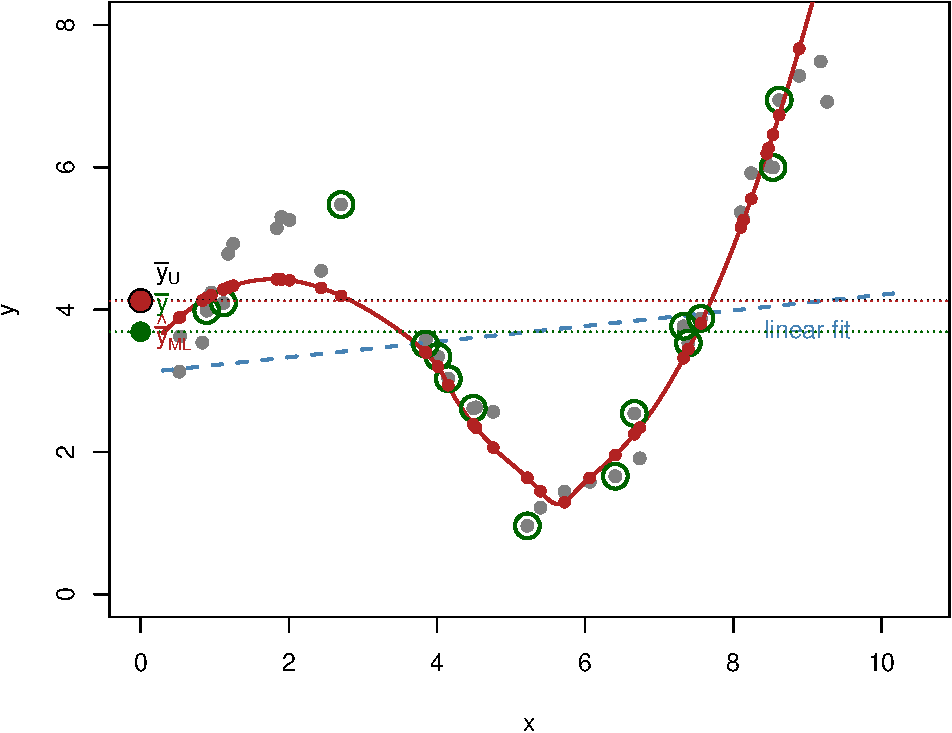
\includegraphics[width=0.7\linewidth,height=\textheight,keepaspectratio]{ratio_files/figure-pdf/fig-ml-concept-1.pdf}

}

\caption{\label{fig-ml-concept}A prediction estimator with a flexible
model. Grey: the population (\(x_i\) known). Green circles: an SRS. Red:
a loess curve fitted to the sample and its predictions for every unit;
blue dashed: a straight-line fit. Left margin: \(\bar y_U\) (black), the
sample mean (green) and the mean of the predictions (red).}

\end{figure}%

Two practical points. Because \(\hat m\) may be nonlinear, the estimator
needs the value \(x_i\) of \textbf{every} population unit, not just
\(\bar x_U\). And there is usually no simple formula for its standard
error, which is then estimated by the bootstrap or by cross-validation
of the residuals.

\section{Simulation study with
agpop.csv}\label{simulation-study-with-agpop.csv}

Let's test this practically by drawing 2000 random samples and seeing
how SRS and Ratio estimators behave under repeated sampling.

\subsection{Information of population
data}\label{information-of-population-data}

We read the population, drop the counties missing \texttt{acres92} or
\texttt{acres87}, and compute the true total \(t_y\) of 1992 acreage,
the known total \(t_x\) of 1987 acreage and the true ratio
\(B = t_y/t_x\) (acreages in thousands).

\begin{Shaded}
\begin{Highlighting}[]
\NormalTok{agpop }\OtherTok{\textless{}{-}} \FunctionTok{acres\_in\_thousands}\NormalTok{(}\FunctionTok{read.csv}\NormalTok{(}\StringTok{"data/agpop.csv"}\NormalTok{))}
\DocumentationTok{\#\# acres87 is the auxiliary variable, so drop counties missing either one}
\NormalTok{agpop }\OtherTok{\textless{}{-}}\NormalTok{ agpop[}\SpecialCharTok{!}\FunctionTok{is.na}\NormalTok{(agpop}\SpecialCharTok{$}\NormalTok{acres92) }\SpecialCharTok{\&} \SpecialCharTok{!}\FunctionTok{is.na}\NormalTok{(agpop}\SpecialCharTok{$}\NormalTok{acres87), ]}

\CommentTok{\# sample size}
\NormalTok{n }\OtherTok{\textless{}{-}} \DecValTok{300}
\CommentTok{\# population size}
\NormalTok{N }\OtherTok{\textless{}{-}} \FunctionTok{nrow}\NormalTok{(agpop)}

\CommentTok{\# true values that we want to estimate}
\NormalTok{tyU }\OtherTok{\textless{}{-}} \FunctionTok{sum}\NormalTok{(agpop[, }\StringTok{"acres92"}\NormalTok{])}
\CommentTok{\# suppose known for ratio estimate}
\NormalTok{txU }\OtherTok{\textless{}{-}} \FunctionTok{sum}\NormalTok{(agpop[, }\StringTok{"acres87"}\NormalTok{]) }
\NormalTok{B }\OtherTok{\textless{}{-}}\NormalTok{ tyU }\SpecialCharTok{/}\NormalTok{ txU}
\end{Highlighting}
\end{Shaded}

The scatter plot of 1992 against 1987 acreage, with the line through the
origin of slope \(B\), shows how well the earlier acreage predicts the
later one.

\begin{Shaded}
\begin{Highlighting}[]
\FunctionTok{plot}\NormalTok{(agpop[, }\StringTok{"acres87"}\NormalTok{], agpop[, }\StringTok{"acres92"}\NormalTok{], }\AttributeTok{main=}\StringTok{"Acres 1992 vs Acres 1987"}\NormalTok{)}
\FunctionTok{abline}\NormalTok{(}\AttributeTok{a =} \DecValTok{0}\NormalTok{, }\AttributeTok{b =}\NormalTok{ B, }\AttributeTok{col=}\StringTok{"red"}\NormalTok{)}
\end{Highlighting}
\end{Shaded}

\begin{figure}[H]

\centering{

\pandocbounded{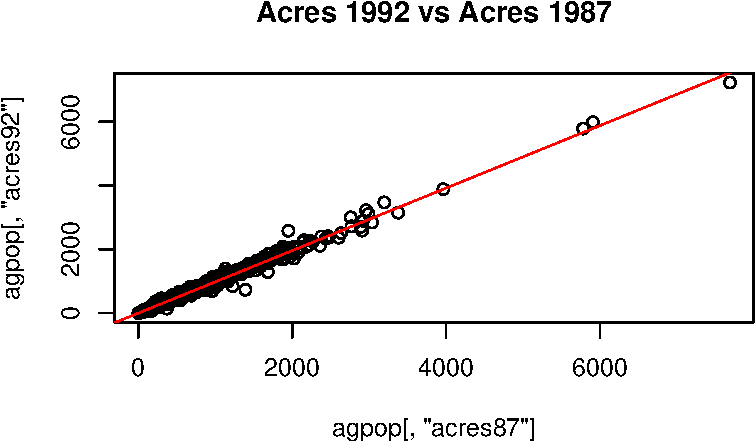
\includegraphics[keepaspectratio]{ratio_files/figure-pdf/fig-agpop-acres8792-ratio-line-1.pdf}}

}

\caption{\label{fig-agpop-acres8792-ratio-line}1992 vs.~1987 county
acreage with the true ratio line}

\end{figure}%

We fit the population line and compute the expected variance reduction
\(1 - S_d^2/S_y^2\) from the population residuals \(d_i = y_i - Bx_i\)
of the theory section.

\begin{Shaded}
\begin{Highlighting}[]
\CommentTok{\# linear model output}
\NormalTok{lm\_gt }\OtherTok{\textless{}{-}} \FunctionTok{format\_lm\_gt}\NormalTok{(}\FunctionTok{lm}\NormalTok{(agpop}\SpecialCharTok{$}\NormalTok{acres92 }\SpecialCharTok{\textasciitilde{}}\NormalTok{ agpop}\SpecialCharTok{$}\NormalTok{acres87))}
\NormalTok{lm\_gt}\SpecialCharTok{$}\NormalTok{coef}
\end{Highlighting}
\end{Shaded}

\begin{table}[H]
\caption*{
{\large  Coefficient Estimates\normalsize }
} 
\normalsize
\begin{gtfit}{0.7\linewidth}{l|rrrr}
\toprule
 & Estimate & S.E. & t value & p value \\ 
\midrule\addlinespace[2.5pt]
(Intercept) & -2.4509 & 0.8517 & -2.8775 & 0.0040 \\ 
agpop\$acres87 & 0.9882 & 0.0016 & 618.4281 & 0.0000 \\ 
\bottomrule
\end{gtfit}
\end{table}

\begin{Shaded}
\begin{Highlighting}[]
\NormalTok{lm\_gt}\SpecialCharTok{$}\NormalTok{fit}
\end{Highlighting}
\end{Shaded}

\begin{table}[H]
\caption*{
{\large  Model Fit Summary\normalsize }
} 
\normalsize
\begin{gtfit}{0.7\linewidth}{rrrrr}
\toprule
\(R^2\) & Adj. \(R^2\) & \(\hat\sigma\) & F-statistic & p-value \\ 
\midrule\addlinespace[2.5pt]
0.9921 & 0.9921 & 37.8382 & 382,453.3759 & 0.0000 \\ 
\bottomrule
\end{gtfit}
\end{table}

\begin{Shaded}
\begin{Highlighting}[]
\CommentTok{\# expected reduction of variance of ratio estimate to srs}
\NormalTok{exp\_var\_red }\OtherTok{\textless{}{-}} \DecValTok{1} \SpecialCharTok{{-}} \FunctionTok{var}\NormalTok{(agpop}\SpecialCharTok{$}\NormalTok{acres92 }\SpecialCharTok{{-}}\NormalTok{ B }\SpecialCharTok{*}\NormalTok{ agpop}\SpecialCharTok{$}\NormalTok{acres87) }\SpecialCharTok{/} \FunctionTok{var}\NormalTok{(agpop}\SpecialCharTok{$}\NormalTok{acres92)}
\NormalTok{exp\_var\_red}
\end{Highlighting}
\end{Shaded}

\begin{verbatim}
[1] 0.9920478
\end{verbatim}

\textbf{Output Note:} Past acreage (1987) strongly predicts current
acreage (1992). The theoretically expected variance reduction is roughly
99.2\%.

\subsection{Simulation Studies}\label{simulation-studies}

Each of the 2000 simulations draws an SRS of \(n = 300\) counties and
computes two estimates of the total 1992 acreage: the SRS estimate
\(N\bar y\) and the ratio estimate \(\hat B\,t_x\). The boxplot compares
their sampling distributions around the true total (red line).

\begin{Shaded}
\begin{Highlighting}[]
\NormalTok{nsim }\OtherTok{\textless{}{-}} \DecValTok{2000}
\NormalTok{sim\_rat }\OtherTok{\textless{}{-}} \FunctionTok{data.frame}\NormalTok{(}\AttributeTok{simple =} \FunctionTok{rep}\NormalTok{(}\DecValTok{0}\NormalTok{, nsim), }\AttributeTok{ratio =} \FunctionTok{rep}\NormalTok{(}\DecValTok{0}\NormalTok{, nsim), }\AttributeTok{B =} \FunctionTok{rep}\NormalTok{(}\DecValTok{0}\NormalTok{, nsim))}

\ControlFlowTok{for}\NormalTok{ (i }\ControlFlowTok{in} \DecValTok{1}\SpecialCharTok{:}\NormalTok{nsim) \{}
\NormalTok{  srs }\OtherTok{\textless{}{-}} \FunctionTok{sample}\NormalTok{(N, n)}
\NormalTok{  y\_srs }\OtherTok{\textless{}{-}}\NormalTok{ agpop[srs, }\StringTok{"acres92"}\NormalTok{]}
\NormalTok{  x\_srs }\OtherTok{\textless{}{-}}\NormalTok{ agpop[srs, }\StringTok{"acres87"}\NormalTok{]}

  \CommentTok{\# SRS estimate (Total)}
\NormalTok{  sim\_rat}\SpecialCharTok{$}\NormalTok{simple[i] }\OtherTok{\textless{}{-}} \FunctionTok{mean}\NormalTok{(y\_srs) }\SpecialCharTok{*}\NormalTok{ N }
  \CommentTok{\# ratio estimate (Total)}
\NormalTok{  sim\_rat}\SpecialCharTok{$}\NormalTok{B[i] }\OtherTok{\textless{}{-}} \FunctionTok{mean}\NormalTok{(y\_srs) }\SpecialCharTok{/} \FunctionTok{mean}\NormalTok{(x\_srs)}
\NormalTok{  sim\_rat}\SpecialCharTok{$}\NormalTok{ratio[i] }\OtherTok{\textless{}{-}}\NormalTok{  sim\_rat}\SpecialCharTok{$}\NormalTok{B[i] }\SpecialCharTok{*}\NormalTok{ txU}
\NormalTok{\}}

\FunctionTok{boxplot}\NormalTok{(sim\_rat[, }\DecValTok{1}\SpecialCharTok{:}\DecValTok{2}\NormalTok{], }\AttributeTok{main=}\StringTok{"Estimator Variance: SRS vs Ratio"}\NormalTok{)}
\FunctionTok{abline}\NormalTok{(}\AttributeTok{h =}\NormalTok{ tyU, }\AttributeTok{col =} \StringTok{"red"}\NormalTok{, }\AttributeTok{lwd=}\DecValTok{2}\NormalTok{)}
\end{Highlighting}
\end{Shaded}

\begin{figure}[H]

\centering{

\pandocbounded{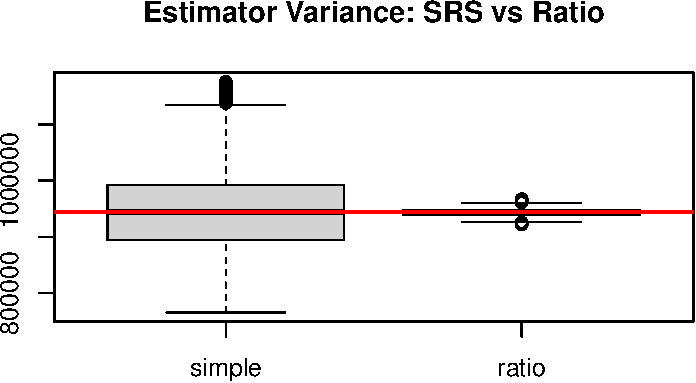
\includegraphics[keepaspectratio]{ratio_files/figure-pdf/fig-agpop-ratio-simulation-boxplot-1.pdf}}

}

\caption{\label{fig-agpop-ratio-simulation-boxplot}Estimator variance
under repeated sampling: SRS vs.~ratio estimator (2000 simulations)}

\end{figure}%

We now calculate the actual variance across our 2000 simulations.

\begin{Shaded}
\begin{Highlighting}[]
\NormalTok{sim\_var }\OtherTok{\textless{}{-}} \FunctionTok{sapply}\NormalTok{(sim\_rat[, }\DecValTok{1}\SpecialCharTok{:}\DecValTok{2}\NormalTok{], var)}
\NormalTok{ratio\_sim\_var }\OtherTok{\textless{}{-}}\NormalTok{ sim\_var }\SpecialCharTok{/}\NormalTok{ sim\_var[}\DecValTok{1}\NormalTok{]}
\NormalTok{percentage\_reduction }\OtherTok{\textless{}{-}} \DecValTok{1} \SpecialCharTok{{-}}\NormalTok{ ratio\_sim\_var}

\FunctionTok{data.frame}\NormalTok{(sim\_var, ratio\_sim\_var, percentage\_reduction) }\SpecialCharTok{|\textgreater{}} 
  \FunctionTok{gt}\NormalTok{(}\AttributeTok{rownames\_to\_stub =} \ConstantTok{TRUE}\NormalTok{) }\SpecialCharTok{|\textgreater{}} 
  \FunctionTok{cols\_label}\NormalTok{(}
    \AttributeTok{sim\_var =} \StringTok{"Variance"}\NormalTok{,}
    \AttributeTok{ratio\_sim\_var =} \StringTok{"Relative Variance"}\NormalTok{,}
    \AttributeTok{percentage\_reduction =} \StringTok{"Variance Reduction"}
\NormalTok{  ) }\SpecialCharTok{|\textgreater{}}
  \FunctionTok{fmt\_number}\NormalTok{(}\AttributeTok{columns =} \FunctionTok{c}\NormalTok{(sim\_var), }\AttributeTok{decimals =} \DecValTok{0}\NormalTok{) }\SpecialCharTok{|\textgreater{}} 
  \FunctionTok{fmt\_percent}\NormalTok{(}\AttributeTok{columns =} \FunctionTok{c}\NormalTok{(percentage\_reduction), }\AttributeTok{decimals =} \DecValTok{2}\NormalTok{) }\SpecialCharTok{|\textgreater{}}
  \FunctionTok{fmt\_number}\NormalTok{(}\AttributeTok{columns =} \FunctionTok{c}\NormalTok{(ratio\_sim\_var), }\AttributeTok{decimals =} \DecValTok{4}\NormalTok{)}
\end{Highlighting}
\end{Shaded}

\begin{table}

\caption{\label{tbl-agpop-ratio-variance-reduction}Simulated variance
and variance reduction: ratio estimator vs.~SRS}

\centering{

\normalsize
\begin{gtfit}{\linewidth}{l|rrr}
\toprule
 & Variance & Relative Variance & Variance Reduction \\ 
\midrule\addlinespace[2.5pt]
simple & 5,168,139,019 & 1.0000 & 0.00\% \\ 
ratio & 40,025,309 & 0.0077 & 99.23\% \\ 
\bottomrule
\end{gtfit}

}

\end{table}%

\textbf{Output Note:} The boxplot dramatically illustrates the precision
gain. The variance of the ratio estimator is only 0.8\% of the SRS
variance, confirming our theoretical expectations.

\bookmarksetup{startatroot}

\chapter{Cluster Sampling}\label{cluster-sampling}

\section{What Is Cluster Sampling?}\label{sec-cluster-intro}

Suppose we want to find out how many bicycles are owned by the residents
of a community of 10,000 households. We could take an SRS of 400
households. Alternatively, we could divide the community into blocks of
about 20 households each, select 20 of the 500 blocks at random, and
then interview every household (or a subsample of the households) in
each selected block. The second plan is an example of \textbf{cluster
sampling}. The blocks are the \textbf{primary sampling units (psus)}, or
\textbf{clusters}. The households are the \textbf{secondary sampling
units (ssus)}; often, as here, the ssus are the elements of the
population.

Why would we sample clusters rather than elements?

\begin{itemize}
\tightlist
\item
  \textbf{A sampling frame of the observation units may be difficult,
  expensive or impossible to construct.} We cannot list all the
  honeybees in a region, or all the customers of a store. A list of the
  individuals in a city may be obtainable only through a list of housing
  units, which is time-consuming and expensive to build.
\item
  \textbf{The population may be widely spread out geographically, or may
  occur in natural clusters} such as households or schools. It is then
  much cheaper to sample clusters than to take an SRS of individuals. To
  survey nursing-home residents, it is far cheaper to sample nursing
  homes and interview every resident in them than to take an SRS of
  residents, which might require travelling to a home to interview just
  one person.
\end{itemize}

The price is usually precision. Figure~\ref{fig-cluster-design}
illustrates a two-stage cluster sample from a synthetic population of
\(N = 10\) clusters of different sizes, from \(M_i = 40\) to \(160\)
units, sorted by their means. Three clusters are selected by SRS
(shaded), and an SRS of \(m_i = 20\) units is taken in each. Only the
selected clusters are observed. When the cluster means differ, as here,
the estimate depends heavily on \emph{which} clusters happen to be
chosen, and a cluster sample is usually less precise than an SRS of the
same number of units.

\begin{figure}

\centering{

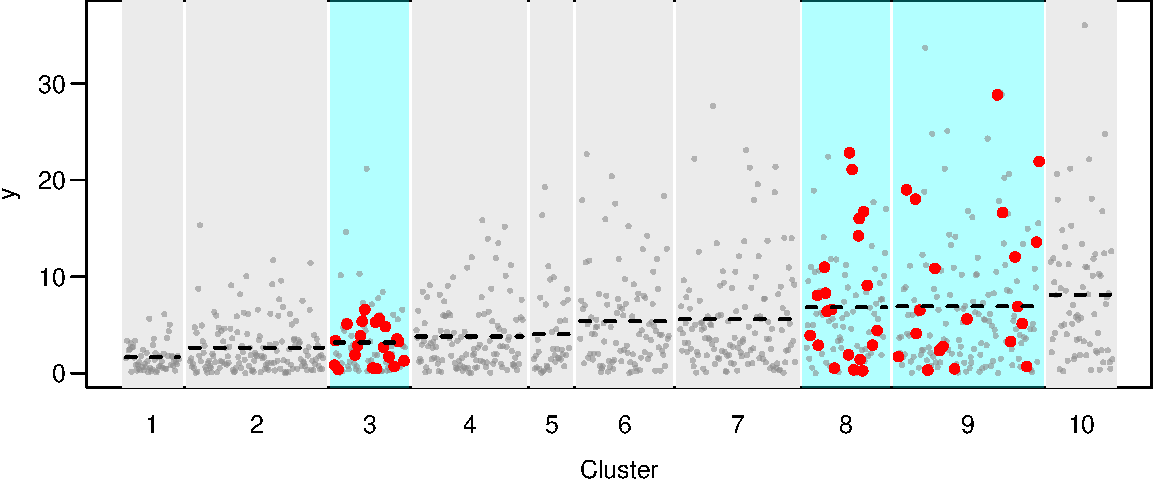
\includegraphics[width=0.85\linewidth,height=\textheight,keepaspectratio]{cluster_files/figure-pdf/fig-cluster-design-1.pdf}

}

\caption{\label{fig-cluster-design}A two-stage cluster sample from a
synthetic population of 10 clusters of 40 to 160 units, sorted by their
means (dashed lines). Three clusters are selected at random (shaded),
and 20 units (red) are subsampled in each; the other clusters are not
observed at all.}

\end{figure}%

The material in this chapter corresponds to Sections 5.1--5.3 of Lohr
and Chapters 8 and 9 of Scheaffer et al.

\subsection{Cluster sampling versus stratified
sampling}\label{cluster-sampling-versus-stratified-sampling}

Both designs partition the population into groups: every element belongs
to exactly one stratum, or to exactly one cluster. The difference is in
how the groups are used (Figure~\ref{fig-cluster-vs-strat}). In
stratified sampling we take an SRS from \emph{every} stratum. In
one-stage cluster sampling we take an SRS of \emph{clusters} and observe
every element in the selected clusters; the other clusters are not
observed at all.

\begin{figure}

\centering{

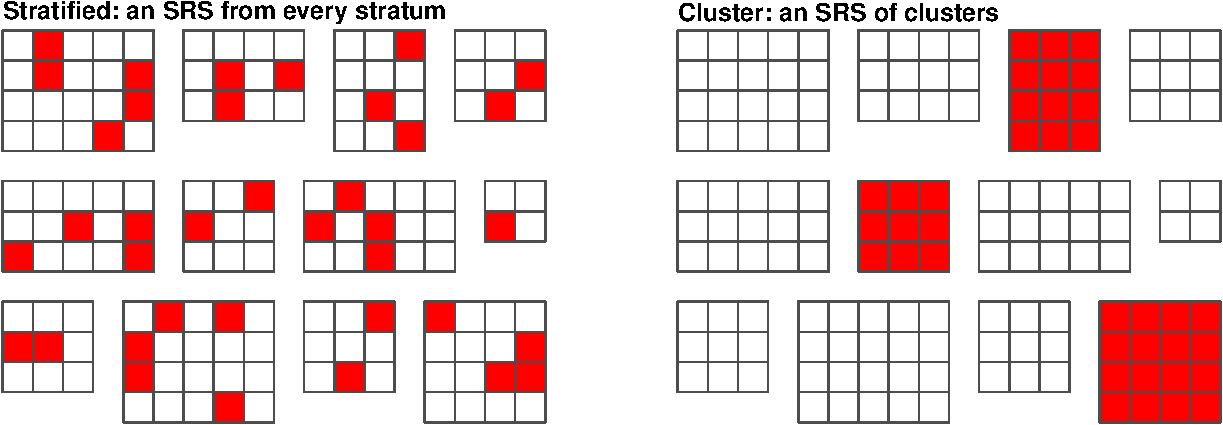
\includegraphics[width=0.95\linewidth,height=\textheight,keepaspectratio]{cluster_files/figure-pdf/fig-cluster-vs-strat-1.pdf}

}

\caption{\label{fig-cluster-vs-strat}The same population of 12 groups of
elements (cells), sampled two ways. Left: stratified sampling takes an
SRS of elements (red) from every stratum. Right: one-stage cluster
sampling takes an SRS of 3 clusters and observes all their elements.}

\end{figure}%

The two designs therefore call for opposite kinds of groups.
Stratification gains precision when each stratum is internally
\emph{homogeneous}, because only the variability within strata enters
the variance. Cluster sampling loses precision when the clusters are
internally homogeneous, because only a few clusters are seen, and the
precision depends mainly on the variability \emph{between} the cluster
means. Ideally, each cluster would be a miniature of the whole
population.

\section{Notation for Cluster Sampling}\label{sec-cluster-notation}

\subsection{Population quantities}\label{population-quantities-2}

In cluster sampling the population \(\mathcal U\) is the population of
\(N\) psus. Note the change from earlier chapters: \textbf{\(N\) is now
the number of psus, not the number of elements.} Psu \(i\) contains
\(M_i\) ssus, and we write \[
y_{ij} = \text{the measurement on the } j\text{th ssu in the } i\text{th psu},
\qquad j = 1, \ldots, M_i,\quad i = 1, \ldots, N .
\] Figure~\ref{fig-cluster-cells} displays the population as a row of
clusters. Each cluster is a column of cells, one cell per ssu, holding
its value \(y_{ij}\). The clusters have different numbers of cells: the
size \(M_i\) of each cluster is written at its bottom, and its total
\(t_i\) at its top.

\begin{figure}

\centering{

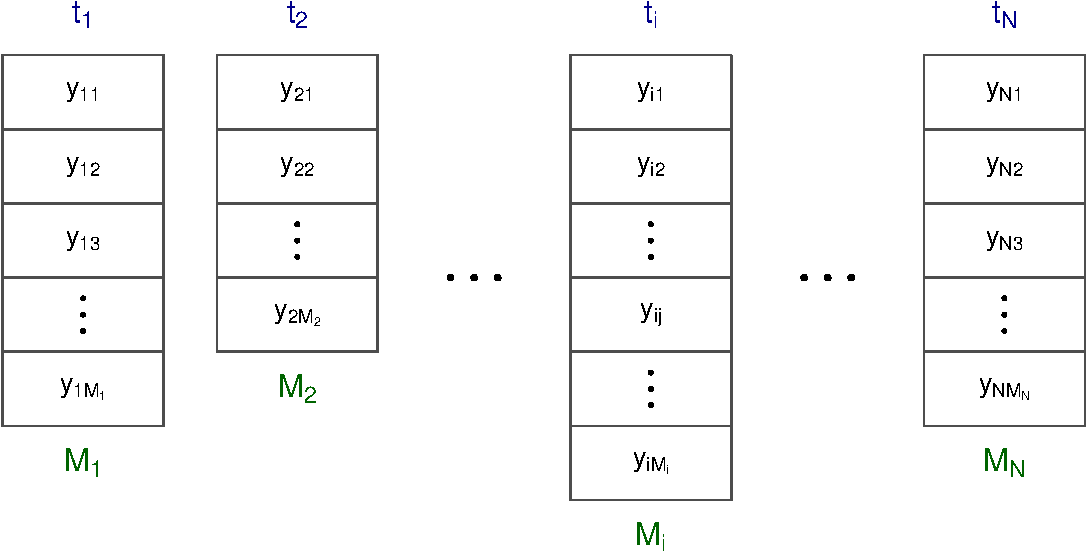
\includegraphics[width=0.75\linewidth,height=\textheight,keepaspectratio]{cluster_files/figure-pdf/fig-cluster-cells-1.pdf}

}

\caption{\label{fig-cluster-cells}The population in cluster sampling.
Cluster (psu) \(i\) is a column of \(M_i\) cells, one per ssu, holding
the values \(y_{i1}, \ldots, y_{iM_i}\). Its total
\(t_i = \sum_j y_{ij}\) is shown at the top and its size \(M_i\) at the
bottom.}

\end{figure}%

The \textbf{psu-level} quantities are the cluster totals and their
spread: \[
t_i = \sum_{j=1}^{M_i} y_{ij} \quad(\text{total in psu } i), \qquad
t = \sum_{i=1}^N t_i \quad(\text{population total}),
\] \[
M_0 = \sum_{i=1}^N M_i \quad(\text{number of ssus}),
\] \[
S_t^2 = \frac{1}{N-1}\sum_{i=1}^N \Big(t_i - \frac tN\Big)^2 \quad(\text{population variance of the psu totals}).
\] The \textbf{ssu-level} quantities describe the individual elements:
\[
\bar y_U = \frac{1}{M_0}\sum_{i=1}^N\sum_{j=1}^{M_i} y_{ij} = \frac{t}{M_0} \quad(\text{population mean per ssu}),
\qquad
\bar y_{iU} = \frac{t_i}{M_i} \quad(\text{mean in psu } i),
\] \[
S^2 = \frac{1}{M_0-1}\sum_{i=1}^N\sum_{j=1}^{M_i}(y_{ij}-\bar y_U)^2 \quad(\text{population variance}),
\] \[
S_i^2 = \frac{1}{M_i-1}\sum_{j=1}^{M_i}(y_{ij}-\bar y_{iU})^2 \quad(\text{variance within psu } i).
\] Here \(\bar y_U\), the mean per element, is usually the quantity of
interest, and \(\bar t_U = t/N\) is the mean per psu.

\subsection{Sample quantities}\label{sample-quantities}

The sample is drawn in up to two stages
(Figure~\ref{fig-cluster-cells-sample}). First an SRS \(\mathcal S\) of
\(n\) psus is drawn from the \(N\) psus. Then, in each sampled psu
\(i\), an SRS \(\mathcal S_i\) of \(m_i\) of its \(M_i\) ssus is drawn.
In \textbf{one-stage} cluster sampling every ssu of a sampled psu is
observed, \(m_i = M_i\); in \textbf{two-stage} cluster sampling
\(m_i < M_i\) for some psus.

\begin{figure}

\centering{

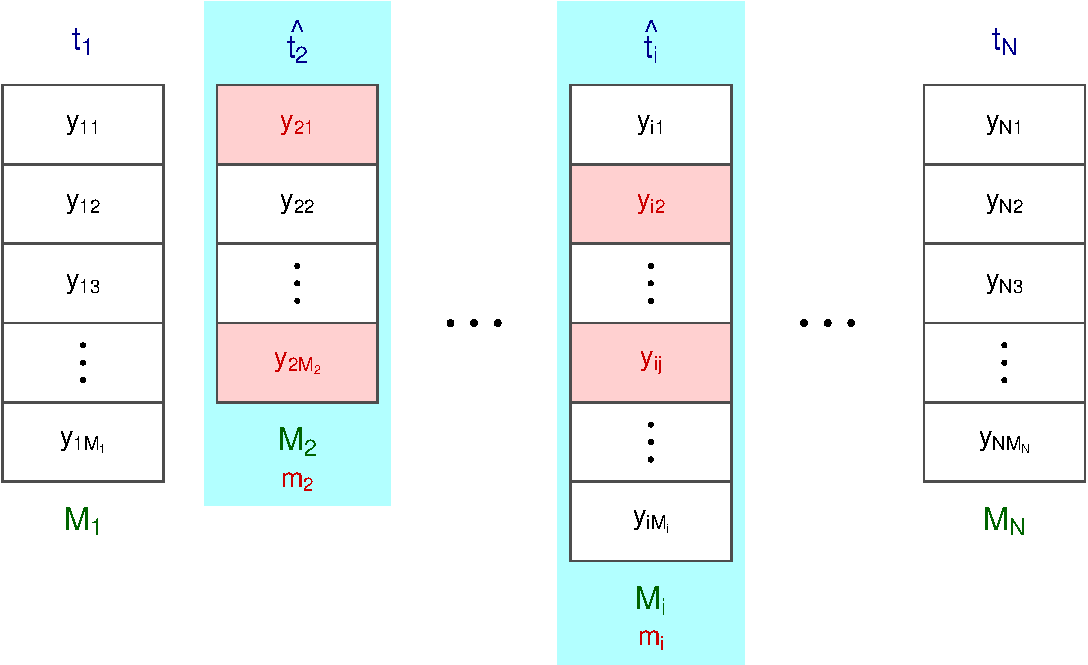
\includegraphics[width=0.75\linewidth,height=\textheight,keepaspectratio]{cluster_files/figure-pdf/fig-cluster-cells-sample-1.pdf}

}

\caption{\label{fig-cluster-cells-sample}A two-stage cluster sample. The
psus \(2\) and \(i\) are in the sample \(\mathcal S\) (shaded); within
each, \(m_i\) of the \(M_i\) ssus are subsampled (red). The psu totals
are not observed and must be estimated, giving \(\hat t_i\).}

\end{figure}%

From the subsample in psu \(i\) we compute the sample mean and the
estimated psu total, \[
\bar y_i = \frac{1}{m_i}\sum_{j\in\mathcal S_i} y_{ij}, \qquad
\hat t_i = \sum_{j\in\mathcal S_i} \frac{M_i}{m_i}y_{ij} = M_i\bar y_i ,
\] and from the \(n\) sampled psus the unbiased estimator of the
population total and the sample variance of the estimated psu totals: \[
\hat t_{\text{unb}} = \frac{N}{n}\sum_{i\in\mathcal S} \hat t_i, \qquad
\bar t = \frac{1}{n}\sum_{i\in\mathcal S} \hat t_i, \qquad
s_t^2 = \frac{1}{n-1}\sum_{i\in\mathcal S} \big(\hat t_i - \bar t\big)^2 .
\] In one-stage sampling \(\hat t_i = t_i\), the true psu total.

\subsection{Sampling weights}\label{sampling-weights}

Ssu \(j\) of psu \(i\) is in the sample if psu \(i\) is selected at the
first stage and ssu \(j\) is selected at the second, so \[
P(\text{ssu } j \text{ of psu } i \text{ is selected})
 = P(\text{psu } i \text{ selected}) \times P(\text{ssu } j \text{ selected} \mid \text{psu } i \text{ selected})
 = \frac nN \cdot \frac{m_i}{M_i}.
\] The sampling weight is the reciprocal, \[
w_{ij} = \frac{N}{n}\cdot\frac{M_i}{m_i}, \qquad
\hat t_{\text{unb}} = \sum_{i\in\mathcal S}\sum_{j\in\mathcal S_i} w_{ij}\,y_{ij} .
\] If the psus are blocks and the ssus are households, household \(j\)
in block \(i\) represents \(NM_i/(nm_i)\) households of the population.

\section{One-Stage Cluster Sampling with Equal Cluster
Sizes}\label{sec-cluster-equal}

Consider first the simplest case: every psu has the same number of ssus,
\(M_i = M\), and all of them are observed, \(m_i = M\). This is uncommon
in household surveys but does occur in agricultural and industrial
sampling. Since every ssu in a sampled psu is observed, the psu totals
\(t_i\) are known for the sampled psus, and we can ignore the individual
elements. \textbf{The design is simply an SRS of \(n\) psu totals}
\(\{t_i, i\in\mathcal S\}\) from the \(N\) psu totals, and the SRS
results of Section~\ref{sec-srs-formulas} apply directly: \[
\hat t = N\bar t = \frac Nn\sum_{i\in\mathcal S} t_i, \qquad
\mathrm{SE}(\hat t) = N\sqrt{\Big(1-\frac nN\Big)\frac{s_t^2}{n}} .
\] The population has \(NM\) elements, so the mean per element is
estimated by \[
\hat{\bar y} = \frac{\hat t}{NM} = \frac{\bar t}{M}, \qquad
\mathrm{SE}(\hat{\bar y}) = \frac{1}{M}\sqrt{\Big(1-\frac nN\Big)\frac{s_t^2}{n}} = \frac{\mathrm{SE}(\bar t)}{M} .
\]

\subsection{Example: GPA in a
dormitory}\label{example-gpa-in-a-dormitory}

A student wants to estimate the average GPA in a dormitory. Instead of
listing all the students and taking an SRS, the student notices that the
dorm consists of \(N = 100\) suites of \(M = 4\) students each. The
student selects \(n = 5\) suites at random and asks every person in them
for their GPA:

\begin{Shaded}
\begin{Highlighting}[]
\NormalTok{gpa }\OtherTok{\textless{}{-}} \FunctionTok{data.frame}\NormalTok{(}
  \AttributeTok{suite =} \FunctionTok{rep}\NormalTok{(}\DecValTok{1}\SpecialCharTok{:}\DecValTok{5}\NormalTok{, }\AttributeTok{each =} \DecValTok{4}\NormalTok{),}
  \AttributeTok{gpa   =} \FunctionTok{c}\NormalTok{(}\FloatTok{3.08}\NormalTok{, }\FloatTok{2.60}\NormalTok{, }\FloatTok{3.44}\NormalTok{, }\FloatTok{3.04}\NormalTok{,  }\FloatTok{2.36}\NormalTok{, }\FloatTok{3.04}\NormalTok{, }\FloatTok{3.28}\NormalTok{, }\FloatTok{2.68}\NormalTok{,  }\FloatTok{2.00}\NormalTok{, }\FloatTok{2.56}\NormalTok{, }\FloatTok{2.52}\NormalTok{, }\FloatTok{1.88}\NormalTok{,}
            \FloatTok{3.00}\NormalTok{, }\FloatTok{2.88}\NormalTok{, }\FloatTok{3.44}\NormalTok{, }\FloatTok{3.64}\NormalTok{,  }\FloatTok{2.68}\NormalTok{, }\FloatTok{1.92}\NormalTok{, }\FloatTok{3.28}\NormalTok{, }\FloatTok{3.20}\NormalTok{)}
\NormalTok{)}
\NormalTok{ti }\OtherTok{\textless{}{-}} \FunctionTok{tapply}\NormalTok{(gpa}\SpecialCharTok{$}\NormalTok{gpa, gpa}\SpecialCharTok{$}\NormalTok{suite, sum)      }\CommentTok{\# suite totals t\_i}
\FunctionTok{matrix}\NormalTok{(gpa}\SpecialCharTok{$}\NormalTok{gpa, }\AttributeTok{nrow =} \DecValTok{5}\NormalTok{, }\AttributeTok{byrow =} \ConstantTok{TRUE}\NormalTok{,}
       \AttributeTok{dimnames =} \FunctionTok{list}\NormalTok{(}\FunctionTok{paste}\NormalTok{(}\StringTok{"Suite"}\NormalTok{, }\DecValTok{1}\SpecialCharTok{:}\DecValTok{5}\NormalTok{), }\FunctionTok{paste}\NormalTok{(}\StringTok{"Person"}\NormalTok{, }\DecValTok{1}\SpecialCharTok{:}\DecValTok{4}\NormalTok{))) }\SpecialCharTok{|\textgreater{}}
  \FunctionTok{cbind}\NormalTok{(}\StringTok{\textasciigrave{}}\AttributeTok{Total t\_i}\StringTok{\textasciigrave{}} \OtherTok{=}\NormalTok{ ti)}
\end{Highlighting}
\end{Shaded}

\begin{verbatim}
        Person 1 Person 2 Person 3 Person 4 Total t_i
Suite 1     3.08     2.60     3.44     3.04     12.16
Suite 2     2.36     3.04     3.28     2.68     11.36
Suite 3     2.00     2.56     2.52     1.88      8.96
Suite 4     3.00     2.88     3.44     3.64     12.96
Suite 5     2.68     1.92     3.28     3.20     11.08
\end{verbatim}

The psus are the suites. Treating the five suite totals as an SRS from
the 100 suite totals,

\begin{Shaded}
\begin{Highlighting}[]
\NormalTok{N }\OtherTok{\textless{}{-}} \DecValTok{100}\NormalTok{; n }\OtherTok{\textless{}{-}} \DecValTok{5}\NormalTok{; M }\OtherTok{\textless{}{-}} \DecValTok{4}
\NormalTok{t\_hat  }\OtherTok{\textless{}{-}}\NormalTok{ N }\SpecialCharTok{/}\NormalTok{ n }\SpecialCharTok{*} \FunctionTok{sum}\NormalTok{(ti)}
\NormalTok{s2\_t   }\OtherTok{\textless{}{-}} \FunctionTok{var}\NormalTok{(ti)}
\NormalTok{ybar   }\OtherTok{\textless{}{-}}\NormalTok{ t\_hat }\SpecialCharTok{/}\NormalTok{ (N }\SpecialCharTok{*}\NormalTok{ M)}
\NormalTok{se\_ybar }\OtherTok{\textless{}{-}} \FunctionTok{sqrt}\NormalTok{((}\DecValTok{1} \SpecialCharTok{{-}}\NormalTok{ n }\SpecialCharTok{/}\NormalTok{ N) }\SpecialCharTok{*}\NormalTok{ s2\_t }\SpecialCharTok{/}\NormalTok{ n) }\SpecialCharTok{/}\NormalTok{ M}
\FunctionTok{c}\NormalTok{(}\AttributeTok{t\_hat =}\NormalTok{ t\_hat, }\AttributeTok{tbar =} \FunctionTok{mean}\NormalTok{(ti), }\AttributeTok{s2\_t =}\NormalTok{ s2\_t, }\AttributeTok{ybar =}\NormalTok{ ybar, }\AttributeTok{SE =}\NormalTok{ se\_ybar)}
\end{Highlighting}
\end{Shaded}

\begin{verbatim}
       t_hat         tbar         s2_t         ybar           SE 
1130.4000000   11.3040000    2.2556800    2.8260000    0.1636649 
\end{verbatim}

\[
\hat t = \frac{100}{5}(12.16+11.36+8.96+12.96+11.08) = 1130.4, \qquad
s_t^2 = 2.256,
\] \[
\hat{\bar y} = \frac{1130.4}{400} = 2.826, \qquad
\mathrm{SE}(\hat{\bar y}) = \sqrt{\Big(1-\frac{5}{100}\Big)\frac{2.256}{(5)(4)^2}} = 0.164 .
\]

The same estimate is obtained by \texttt{srs\_est()} applied to the
suite totals, divided by \(M\):

\begin{Shaded}
\begin{Highlighting}[]
\FunctionTok{srs\_est}\NormalTok{(ti }\SpecialCharTok{/}\NormalTok{ M, }\AttributeTok{N =}\NormalTok{ N, }\AttributeTok{estimate =} \StringTok{"mean"}\NormalTok{, }\AttributeTok{show.details =} \ConstantTok{FALSE}\NormalTok{)}\SpecialCharTok{$}\NormalTok{estimate }\SpecialCharTok{|\textgreater{}} \FunctionTok{format\_est\_gt}\NormalTok{(}\StringTok{"mean"}\NormalTok{)}
\end{Highlighting}
\end{Shaded}

\begin{table}[H]
\normalsize
\begin{gtfit}{0.7\linewidth}{rrrr}
\toprule
\(\bar{y}\) & \(\mathrm{SE}(\bar{y})\) & 95\% CI Lower & 95\% CI Upper \\ 
\midrule\addlinespace[2.5pt]
2.83 & 0.16 & 2.37 & 3.28 \\ 
\bottomrule
\end{gtfit}
\end{table}

(The confidence interval here uses \(t_{0.025,\,4}\), since only
\(n = 5\) suites were sampled.)

\textbf{Do not use the SRS formula for the 20 students.} It is tempting
to treat the \(nM = 20\) students as an SRS from the 400 students in the
dorm:

\begin{Shaded}
\begin{Highlighting}[]
\NormalTok{se\_naive }\OtherTok{\textless{}{-}} \FunctionTok{sqrt}\NormalTok{((}\DecValTok{1} \SpecialCharTok{{-}} \DecValTok{20} \SpecialCharTok{/} \DecValTok{400}\NormalTok{) }\SpecialCharTok{*} \FunctionTok{var}\NormalTok{(gpa}\SpecialCharTok{$}\NormalTok{gpa) }\SpecialCharTok{/} \DecValTok{20}\NormalTok{)}
\FunctionTok{c}\NormalTok{(}\AttributeTok{SE\_cluster =}\NormalTok{ se\_ybar, }\AttributeTok{SE\_naive\_SRS =}\NormalTok{ se\_naive)}
\end{Highlighting}
\end{Shaded}

\begin{verbatim}
  SE_cluster SE_naive_SRS 
   0.1636649    0.1121526 
\end{verbatim}

The naive standard error, 0.112, is much smaller than the correct 0.164.
The 20 students are not an SRS of students: whole suites are selected
together, and students in the same suite tend to have similar GPAs.
Treating them as independent observations overstates the information in
the sample. The next section makes this precise.

\section{Comparing Cluster Sampling with SRS}\label{sec-cluster-vs-srs}

How much precision do we lose by sampling clusters instead of elements?
For equal-sized clusters the answer comes from the analysis-of-variance
decomposition of the population, with the clusters playing the role of
groups:

{\def\LTcaptype{none} % do not increment counter
\begin{longtable}[]{@{}
  >{\raggedright\arraybackslash}p{(\linewidth - 4\tabcolsep) * \real{0.3077}}
  >{\centering\arraybackslash}p{(\linewidth - 4\tabcolsep) * \real{0.3846}}
  >{\raggedright\arraybackslash}p{(\linewidth - 4\tabcolsep) * \real{0.3077}}@{}}
\toprule\noalign{}
\begin{minipage}[b]{\linewidth}\raggedright
Source
\end{minipage} & \begin{minipage}[b]{\linewidth}\centering
df
\end{minipage} & \begin{minipage}[b]{\linewidth}\raggedright
Sum of squares
\end{minipage} \\
\midrule\noalign{}
\endhead
\bottomrule\noalign{}
\endlastfoot
Between psus & \(N-1\) &
\(\text{SSB} = \sum_{i=1}^N\sum_{j=1}^M (\bar y_{iU}-\bar y_U)^2\) \\
Within psus & \(N(M-1)\) &
\(\text{SSW} = \sum_{i=1}^N\sum_{j=1}^M (y_{ij}-\bar y_{iU})^2\) \\
Total, about \(\bar y_U\) & \(NM-1\) &
\(\text{SSTO} = \sum_{i=1}^N\sum_{j=1}^M (y_{ij}-\bar y_U)^2 = (NM-1)S^2\) \\
\end{longtable}
}

with mean squares \(\text{MSB} = \text{SSB}/(N-1)\) and
\(\text{MSW} = \text{SSW}/(N(M-1))\).

\textbf{The variance depends on the between-psu variability.} Since
every psu has size \(M\),
\(t_i - \bar t_U = M(\bar y_{iU} - \bar y_U)\), so \[
S_t^2 = \frac{1}{N-1}\sum_{i=1}^N (t_i-\bar t_U)^2 = \frac{M}{N-1}\sum_{i=1}^N M(\bar y_{iU}-\bar y_U)^2 = M\cdot\text{MSB},
\] and the variance of the estimated total from one-stage cluster
sampling is \[
V(\hat t_{\text{cluster}}) = N^2\Big(1-\frac nN\Big)\frac{S_t^2}{n} = N^2\Big(1-\frac nN\Big)\frac{M\cdot\text{MSB}}{n}.
\] An SRS of the same number \(nM\) of elements, from the \(NM\)
elements, would give \[
V(\hat t_{\text{SRS}}) = (NM)^2\Big(1-\frac{nM}{NM}\Big)\frac{S^2}{nM} = N^2\Big(1-\frac nN\Big)\frac{M S^2}{n}.
\] The ratio of the two variances is therefore \[
\frac{V(\hat t_{\text{cluster}})}{V(\hat t_{\text{SRS}})} = \frac{\text{MSB}}{S^2}.
\] If \(\text{MSB} > S^2\), that is, if the cluster means vary more than
would be expected from randomly formed groups, cluster sampling is
\textbf{less efficient} than an SRS of the same number of elements.

\subsection{\texorpdfstring{Intraclass correlation and adjusted
\(R^2\)}{Intraclass correlation and adjusted R\^{}2}}\label{intraclass-correlation-and-adjusted-r2}

Two measures of how similar the elements within a cluster are, compared
with elements from different clusters, are the \textbf{intraclass
correlation coefficient} \[
\text{ICC} = 1 - \frac{M}{M-1}\cdot\frac{\text{SSW}}{\text{SSTO}},
\] and the \textbf{adjusted \(R^2\)}, which also applies to clusters of
unequal sizes, \[
R_a^2 = 1 - \frac{\text{MSW}}{S^2}.
\] Both are close to 0 when the clusters are like random groups of
elements, and close to 1 when the elements within each cluster are
nearly identical. For equal-sized clusters, the variance ratio can be
written in terms of \(R_a^2\): \[
\frac{V(\hat t_{\text{cluster}})}{V(\hat t_{\text{SRS}})} = \frac{\text{MSB}}{S^2} = 1 + \frac{N(M-1)}{N-1}R_a^2 \approx 1 + (M-1)R_a^2 .
\] So \((M-1)R_a^2\) is approximately the proportional increase in
variance from using cluster sampling instead of an SRS of the same size.
Even a small \(R_a^2\) matters when the clusters are large: with
\(M = 21\) elements per cluster and \(R_a^2 = 0.05\), the variance
doubles.

\begin{figure}

\centering{

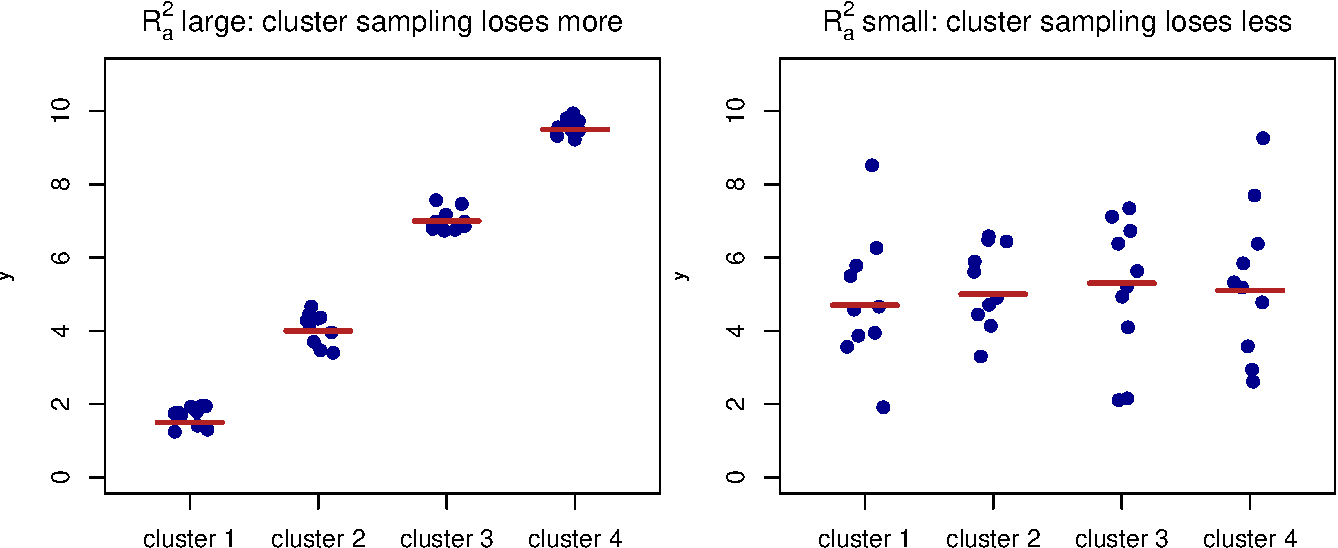
\includegraphics[width=0.9\linewidth,height=\textheight,keepaspectratio]{cluster_files/figure-pdf/fig-cluster-r2-1.pdf}

}

\caption{\label{fig-cluster-r2}Left: the cluster means differ a lot
relative to the spread within the clusters (\(R_a^2\) large), so
sampling a few clusters misses most of the population's variability and
cluster sampling loses much precision. Right: the clusters look like
random groups (\(R_a^2\) small), and cluster sampling loses little.}

\end{figure}%

This is the mirror image of stratification
(Section~\ref{sec-strata-prop}). There, a large \(R^2\) between strata
\emph{reduces} the variance, because every stratum is sampled. Here, a
large \(R_a^2\) between clusters \emph{increases} the variance, because
most clusters are not sampled.

\section{One-Stage Cluster Sampling with Unequal Cluster
Sizes}\label{sec-cluster-unequal}

In most surveys the clusters have different sizes: classes have
different numbers of students, and counties different numbers of farms.

\subsection{The unbiased estimator}\label{the-unbiased-estimator}

The unbiased estimator of the total is computed exactly as before, \[
\hat t_{\text{unb}} = \frac Nn \sum_{i\in\mathcal S} t_i, \qquad
\mathrm{SE}(\hat t_{\text{unb}}) = N\sqrt{\Big(1-\frac nN\Big)\frac{s_t^2}{n}},
\] and \(\hat t_{\text{unb}}/M_0\) is unbiased for \(\bar y_U\) when
\(M_0\) is known. But now the cluster totals \(t_i\) vary for two
reasons. A psu with many ssus tends to have a large total simply because
it has more elements, quite apart from any differences in the
\(y\)-values. When the cluster sizes differ a lot, this inflates
\(s_t^2\), and with it the variance of \(\hat t_{\text{unb}}\).

\subsection{The ratio estimator}\label{the-ratio-estimator-1}

Since \(\bar y_U = t/M_0\), and \(t_i\) is usually roughly proportional
to \(M_i\), estimating \(\bar y_U\) is a \textbf{ratio estimation}
problem (see the ratio chapter) with \(y\)-variable \(t_i\) and
auxiliary variable \(x_i = M_i\): \[
\boxed{
\hat{\bar y}_r = \frac{\sum_{i\in\mathcal S} t_i}{\sum_{i\in\mathcal S} M_i} = \frac{\sum_{i\in\mathcal S} M_i\bar y_i}{\sum_{i\in\mathcal S} M_i} .}
\] It is the total of the sampled elements divided by their number, a
weighted average of the cluster means with weights \(M_i\). Its standard
error follows from the ratio-estimator formula with \(x_i = M_i\): \[
\boxed{
\mathrm{SE}(\hat{\bar y}_r) = \sqrt{\Big(1-\frac nN\Big)\frac{s_e^2}{n\bar M^2}}, \qquad
s_e^2 = \frac{1}{n-1}\sum_{i\in\mathcal S}e_i^2, \qquad e_i = t_i-\hat{\bar y}_r M_i ,}
\] where \(\bar M = \sum_{i\in\mathcal S}M_i/n\) is the average size of
the sampled clusters. The residuals \(e_i\) measure how far each cluster
total lies from the line \(t = \hat{\bar y}_r M\) through the origin
(Figure~\ref{fig-cluster-ratio}). They are typically far less variable
than the deviations \(t_i - \bar t\) about the horizontal line
\(\bar t\), which determine \(s_t^2\) and hence the standard error of
the unbiased estimator, because the size-driven part of the variation
has been removed. Note that the ratio estimator does not need \(M_0\),
the total number of elements in the population.

\begin{figure}

\centering{

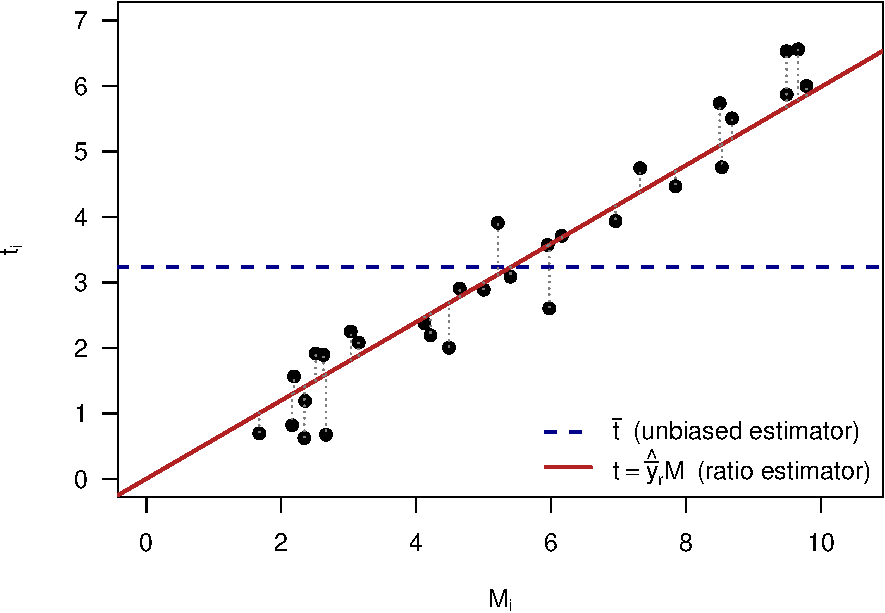
\includegraphics[width=0.6\linewidth,height=\textheight,keepaspectratio]{cluster_files/figure-pdf/fig-cluster-ratio-1.pdf}

}

\caption{\label{fig-cluster-ratio}Cluster totals \(t_i\) against cluster
sizes \(M_i\). The unbiased estimator's standard error depends on the
spread of the \(t_i\) about their mean \(\bar t\) (blue dashed line),
which is large because the sizes vary. The ratio estimator uses the line
\(t = \hat{\bar y}_r M\) (red), and its standard error depends only on
the residuals about that line (dotted).}

\end{figure}%

\subsection{A toy example: why the unbiased estimator can be
bad}\label{a-toy-example-why-the-unbiased-estimator-can-be-bad}

Consider a whimsical population of just \(N = 2\) clusters (kennels) of
dogs: kennel A with \(M_A = 30\) dogs and kennel B with \(M_B = 10\)
dogs. Every dog has exactly 4 legs, so the mean number of legs per dog
is \(\bar y_U = 4\), and \(M_0 = 40\). We take a one-stage cluster
sample of \(n = 1\) kennel, each kennel being chosen with probability
\(1/2\).

\textbf{The unbiased estimator.} If kennel A is selected,
\(t_A = 30\times 4 = 120\), \(\hat t_{\text{unb}} = \frac21(120) = 240\)
and \(\hat{\bar y}_{\text{unb}} = 240/40 = 6\). If kennel B is selected,
\(t_B = 40\), \(\hat t_{\text{unb}} = 80\) and
\(\hat{\bar y}_{\text{unb}} = 80/40 = 2\). So \[
E[\hat{\bar y}_{\text{unb}}] = 6\times\tfrac12 + 2\times\tfrac12 = 4 = \bar y_U ,
\] and the estimator is unbiased. But it is \emph{never} equal to 4: it
is always off by 2, even though every dog has exactly 4 legs. All of its
variance comes from the different kennel sizes.

\textbf{The ratio estimator.} If kennel A is selected,
\(\hat{\bar y}_r = (30\times 4)/30 = 4\); if kennel B is selected,
\(\hat{\bar y}_r = (10\times4)/10 = 4\). Both possible samples give
exactly the right answer, and \(V(\hat{\bar y}_r) = 0\). The ratio
estimator removes the cluster-size variability that made
\(\hat{\bar y}_{\text{unb}}\) so unreliable. This is why ratio
estimation, not unbiased estimation, is the standard method for clusters
of unequal sizes.

\subsection{Example: algebra class test scores
(algebra.csv)}\label{sec-cluster-algebra}

One-stage cluster samples are common in educational studies, since
students are naturally clustered into classes and schools. Consider a
population of 187 high school algebra classes in a city. An investigator
takes an SRS of \(n = 12\) classes and tests every student in them on
their knowledge of functions. The classes are the psus, of different
sizes \(M_i\), and the students are the ssus.

\begin{Shaded}
\begin{Highlighting}[]
\NormalTok{algebra }\OtherTok{\textless{}{-}} \FunctionTok{read.csv}\NormalTok{(}\StringTok{"data/algebra.csv"}\NormalTok{)}

\FunctionTok{book\_table}\NormalTok{(algebra) }\SpecialCharTok{|\textgreater{}}
  \FunctionTok{tab\_header}\NormalTok{(}\AttributeTok{title =} \StringTok{"Raw Data: Algebra Classes"}\NormalTok{) }\SpecialCharTok{|\textgreater{}}
  \FunctionTok{cols\_label}\NormalTok{(}\AttributeTok{Mi =} \FunctionTok{md}\NormalTok{(}\StringTok{"*M*\textasciitilde{}i\textasciitilde{}"}\NormalTok{))}
\end{Highlighting}
\end{Shaded}

\begin{table}

\caption{\label{tbl-algebra-raw-data}Raw data: algebra classes (sample)}

\centering{

\caption*{
{\large  Raw Data: Algebra Classes\normalsize }
} 
\normalsize
\begin{gtfit}{\linewidth}{rrr}
\toprule
class & \emph{M}\textsubscript{i} & score \\ 
\midrule\addlinespace[2.5pt]
23 & 20 & 57 \\ 
23 & 20 & 90 \\ 
23 & 20 & 56 \\ 
23 & 20 & 57 \\ 
23 & 20 & 46 \\ 
23 & 20 & 55 \\ 
23 & 20 & 62 \\ 
23 & 20 & 66 \\ 
23 & 20 & 78 \\ 
23 & 20 & 76 \\ 
\bottomrule
\end{gtfit}
\begin{minipage}{\linewidth}
\vspace{.05em}
Showing the first 10 of 299 rows; the full table is in the HTML version of the book.\\
\end{minipage}

}

\end{table}%

The function \texttt{cluster\_ratio()} (from
\texttt{samplingestimate.r}) aggregates the data to one row per class
and builds the ratio-estimation working table: the class size \(M_i\),
the class total \(t_i\), the fitted total \(\hat{\bar y}_r M_i\), and
the residual \(e_i\) and its square.

\begin{Shaded}
\begin{Highlighting}[]
\NormalTok{alg\_res }\OtherTok{\textless{}{-}} \FunctionTok{cluster\_ratio}\NormalTok{(}\AttributeTok{data =}\NormalTok{ algebra,}
                         \AttributeTok{cname =} \StringTok{"class"}\NormalTok{,}
                         \AttributeTok{csize =} \StringTok{"Mi"}\NormalTok{,}
                         \AttributeTok{yvar =} \StringTok{"score"}\NormalTok{,}
                         \AttributeTok{N =} \DecValTok{187}\NormalTok{)}
\NormalTok{alg\_res}\SpecialCharTok{$}\NormalTok{table}
\end{Highlighting}
\end{Shaded}

\begin{table}[H]
\caption*{
{\large  Ratio Estimation: Working Table\normalsize } \\ 
{\normalsize  \(n = 12\)\normalsize }
} 
\normalsize
\begin{gtfit}{\linewidth}{>{\raggedright\arraybackslash}p{\dimexpr 30.00pt -2\tabcolsep-1.5\arrayrulewidth}>{\raggedleft\arraybackslash}p{\dimexpr 75.00pt -2\tabcolsep-1.5\arrayrulewidth}>{\raggedleft\arraybackslash}p{\dimexpr 75.00pt -2\tabcolsep-1.5\arrayrulewidth}>{\raggedleft\arraybackslash}p{\dimexpr 75.00pt -2\tabcolsep-1.5\arrayrulewidth}>{\raggedleft\arraybackslash}p{\dimexpr 75.00pt -2\tabcolsep-1.5\arrayrulewidth}>{\raggedleft\arraybackslash}p{\dimexpr 75.00pt -2\tabcolsep-1.5\arrayrulewidth}>{\raggedleft\arraybackslash}p{\dimexpr 75.00pt -2\tabcolsep-1.5\arrayrulewidth}}
\toprule
\(i\) & \(\bar y_i\) & \(\hat t_i\)\textsuperscript{\textit{1}} & \(M_i\) & \(\hat B M_i\)\textsuperscript{\textit{2}} & \(e_i\) & \(e_i^2\) \\ 
\midrule\addlinespace[2.5pt]
1 & 61.50 & 1,230.00 & 20.00 & 1,251.37 & -21.37 & 456.73 \\ 
2 & 64.23 & 1,670.00 & 26.00 & 1,626.78 & 43.22 & 1,867.74 \\ 
3 & 58.42 & 1,402.00 & 24.00 & 1,501.65 & -99.65 & 9,929.22 \\ 
4 & 58.00 & 1,972.00 & 34.00 & 2,127.33 & -155.33 & 24,127.75 \\ 
5 & 58.00 & 1,508.00 & 26.00 & 1,626.78 & -118.78 & 14,109.31 \\ 
6 & 64.86 & 1,816.00 & 28.00 & 1,751.92 & 64.08 & 4,106.28 \\ 
... & ... & ... & ... & ... & ... & ... \\ 
{\bfseries Sum} & {\bfseries ...} & {\bfseries 18,708.00} & {\bfseries 299.00} & {\bfseries 18,708.00} & {\bfseries 0.00} & {\bfseries 194,827.04} \\ 
\bottomrule
\end{gtfit}
\begin{minipage}{\linewidth}
\vspace{.05em}
\textsuperscript{\textit{1}}\(\hat t_i = \bar y_i \, M_i\).\\
\textsuperscript{\textit{2}}\(\hat B = \sum_i \hat t_i / \sum_i M_i = 62.57\), \(\hat B M_i = \hat B\, M_i\), \(s_e^2 = 17,711.55\).\\
\(\bar y_r = \dfrac{\sum_i \hat t_i}{\sum_i M_i} = \dfrac{18,708.00}{299.00} = 62.57\)\\
\(\mathrm{SE}(\bar y_r) = \dfrac{1}{\bar x}\sqrt{\left(1-\dfrac{n}{N}\right)\dfrac{s_e^2}{n}} = \dfrac{1}{24.92}\sqrt{\left(1-\dfrac{12}{187}\right)\dfrac{17,711.55}{12}} = 1.49\)\\
\end{minipage}
\end{table}

The Sum row gives \(\sum M_i\), \(\sum t_i\) and \(\sum e_i^2\), from
which \[
\hat{\bar y}_r = \frac{\sum t_i}{\sum M_i}, \qquad
s_e^2 = \frac{\sum e_i^2}{n-1}, \qquad
\bar M = \frac{\sum M_i}{12}, \qquad
\mathrm{SE}(\hat{\bar y}_r) = \sqrt{\Big(1-\frac{12}{187}\Big)\frac{s_e^2}{12\,\bar M^2}} .
\]

\begin{Shaded}
\begin{Highlighting}[]
\NormalTok{alg\_res}\SpecialCharTok{$}\NormalTok{estimate }\SpecialCharTok{|\textgreater{}} \FunctionTok{format\_est\_gt}\NormalTok{(}\StringTok{"ratio\_mean"}\NormalTok{)}
\end{Highlighting}
\end{Shaded}

\begin{table}[H]
\normalsize
\begin{gtfit}{0.7\linewidth}{rrrr}
\toprule
\(\bar{y}_{r}\) & \(\mathrm{SE}(\bar{y}_{r})\) & 95\% CI Lower & 95\% CI Upper \\ 
\midrule\addlinespace[2.5pt]
62.57 & 1.49 & 59.29 & 65.85 \\ 
\bottomrule
\end{gtfit}
\end{table}

The estimated mean score of a student in the 187 classes is 62.57, with
standard error 1.49 and 95\% confidence interval {[}59.29, 65.85{]}. The
interval uses \(n - 1 = 11\) degrees of freedom: the classes, not the
students, are the units that were randomized.

\section{Two-Stage Cluster Sampling}\label{sec-cluster-two-stage}

Observing every ssu in a sampled psu can be wasteful: if the elements in
a cluster are similar, measuring a few of them tells us almost as much
as measuring all. In \textbf{two-stage cluster sampling} we

\begin{enumerate}
\def\labelenumi{\arabic{enumi}.}
\tightlist
\item
  select an SRS \(\mathcal S\) of \(n\) psus from the \(N\) psus, and
\item
  select an SRS \(\mathcal S_i\) of \(m_i\) ssus from each selected psu
  \(i\).
\end{enumerate}

The psu totals are no longer observed and are estimated by
\(\hat t_i = M_i\bar y_i\) (Figure~\ref{fig-cluster-cells-sample}).

\subsection{The unbiased estimator}\label{the-unbiased-estimator-1}

The unbiased estimator of the total is \[
\hat t_{\text{unb}} = \frac Nn \sum_{i\in\mathcal S} \hat t_i
 = \sum_{i\in\mathcal S}\sum_{j\in\mathcal S_i} w_{ij}y_{ij}, \qquad w_{ij} = \frac{NM_i}{nm_i}.
\] Its variance now has two sources: the variability \emph{between}
psus, from selecting only some of them, and the variability
\emph{within} psus, from subsampling: \[
V(\hat t_{\text{unb}}) = \underbrace{N^2\Big(1-\frac nN\Big)\frac{S_t^2}{n}}_{\text{between psus}}
 + \underbrace{\frac Nn \sum_{i=1}^N \Big(1-\frac{m_i}{M_i}\Big)M_i^2\frac{S_i^2}{m_i}}_{\text{within psus}} .
\] The first term is exactly the one-stage variance. The second term is
the extra cost of not observing every ssu in each sampled psu; it
vanishes when \(m_i = M_i\).

\subsection{The ratio estimator}\label{the-ratio-estimator-2}

As in one-stage sampling, the mean per element is estimated by a ratio
estimator, now with the estimated psu totals \(\hat t_i = M_i\bar y_i\):
\[
\boxed{
\hat{\bar y}_r = \frac{\sum_{i\in\mathcal S}\hat t_i}{\sum_{i\in\mathcal S}M_i} = \frac{\sum_{i\in\mathcal S}M_i\bar y_i}{\sum_{i\in\mathcal S}M_i} .}
\] Its estimated variance is \[
\hat V(\hat{\bar y}_r) = \frac{1}{\bar M^2}\Big(1-\frac nN\Big)\frac{s_e^2}{n}
 + \frac{1}{nN\bar M^2}\sum_{i\in\mathcal S}M_i^2\Big(1-\frac{m_i}{M_i}\Big)\frac{s_i^2}{m_i},
\qquad e_i = \hat t_i - \hat{\bar y}_r M_i ,
\] where \(s_i^2\) is the sample variance of the \(m_i\) elements
measured in psu \(i\).

The two terms have a useful interpretation. Writing
\(M = \sum_{i\in\mathcal S}M_i = n\bar M\) for the number of elements in
the sampled psus, the variance splits into the variance of a
\textbf{ratio} estimate computed over the \(n\) sampled clusters, plus
the cluster sampling fraction \(n/N\) times the variance of a
\textbf{stratified} sample in which those same clusters are the strata:
\[
\hat{V}(\hat{\bar y}_r) =
\underbrace{\left(1 - \frac{n}{N}\right) \frac{1}{n\bar{M}^2}
  \frac{\sum_{i\in\mathcal S} (\hat{t}_i - \hat{\bar y}_r M_i)^2}{n-1}}_{\textstyle \hat{V}_{\mathrm{ratio}}}
\;+\;
\frac{n}{N}
\underbrace{\sum_{i\in\mathcal S} \left(\frac{M_i}{M}\right)^{2}
  \left(1 - \frac{m_i}{M_i}\right)\frac{s_i^2}{m_i}}_{\textstyle \hat{V}_{\mathrm{str}}} .
\] \(\hat{V}_{\mathrm{ratio}}\) is exactly the ratio-estimate variance
for \(\sum \hat{t}_i / \sum M_i\), and \(\hat{V}_{\mathrm{str}}\) is
exactly the stratified variance \(\sum_h W_h^2(1 - n_h/N_h)s_h^2/n_h\)
with the sampled clusters as strata: stratum sizes \(N_h = M_i\), sample
sizes \(n_h = m_i\), and weights \(W_h = M_i/M\). Each term
\[\hat{v}_i = \left(\frac{M_i}{M}\right)^{2}\left(1 - \frac{m_i}{M_i}\right)\frac{s_i^2}{m_i}\]
is one stratum's contribution; the working tables below carry them in a
\(\hat{v}_i\) column whose Sum is \(\hat{V}_{\mathrm{str}}\).

Why is the second piece there at all? If we could see the true cluster
totals \(t_i\), the ratio piece alone would be the whole variance.
Subsampling replaces \(t_i\) by the estimate \(\hat{t}_i\), and the
between-cluster sum of squares absorbs only the fraction \(1 - n/N\) of
the noise that this creates; the stratified piece pays the rest. Three
special cases follow straight from the formula:

\begin{itemize}
\tightlist
\item
  \textbf{One-stage sampling} (\(m_i = M_i\)): every \(\hat{v}_i = 0\),
  and only the ratio piece survives, as in
  Section~\ref{sec-cluster-unequal}.
\item
  \textbf{\(N\) unknown or effectively infinite}: \(n/N \to 0\), the
  stratified piece drops out, and \(s_e^2\) alone does the whole job. In
  practice the second term is often negligible compared with the first.
\item
  \textbf{A census of clusters} (\(n = N\)): the factor \(1 - n/N\)
  kills the ratio piece and \(n/N = 1\) leaves
  \(\hat{V}(\hat{\bar y}_r) = \hat{V}_{\mathrm{str}}\) exactly. Drawing
  every cluster \emph{is} stratified sampling, and the formula says so.
\end{itemize}

\subsection{Example: American coot egg volumes
(coots.csv)}\label{sec-cluster-coots}

The data come from Arnold's (1991) study of the size and volume of
American coot eggs in Minnedosa, Manitoba. The clutches (nests) are the
psus and the eggs are the ssus. From each of \(n = 184\) clutches, two
eggs were measured; the clutch sizes \(M_i\) are known.

\begin{Shaded}
\begin{Highlighting}[]
\NormalTok{coots }\OtherTok{\textless{}{-}} \FunctionTok{read.csv}\NormalTok{(}\StringTok{"data/coots.csv"}\NormalTok{)}
\FunctionTok{book\_table}\NormalTok{(coots)}
\end{Highlighting}
\end{Shaded}

\begin{table}

\caption{\label{tbl-coots-raw-data}Raw data: coot egg clutches (sample)}

\centering{

\normalsize
\begin{gtfit}{\linewidth}{rrrrrr}
\toprule
clutch & csize & length & breadth & volume & tmt \\ 
\midrule\addlinespace[2.5pt]
1 & 13 & 44.30 & 31.10 & 3.7957569 & 1 \\ 
1 & 13 & 45.90 & 32.70 & 3.9328497 & 1 \\ 
2 & 13 & 49.20 & 34.40 & 4.2156036 & 1 \\ 
2 & 13 & 48.70 & 32.70 & 4.1727621 & 1 \\ 
3 & 6 & 51.05 & 34.25 & 0.9317646 & 0 \\ 
3 & 6 & 49.35 & 34.40 & 0.9007362 & 0 \\ 
4 & 11 & 49.20 & 31.55 & 3.0182724 & 1 \\ 
4 & 11 & 48.55 & 33.10 & 2.9783969 & 1 \\ 
5 & 10 & 49.40 & 34.55 & 2.5045800 & 1 \\ 
5 & 10 & 49.05 & 34.95 & 2.4868350 & 1 \\ 
\bottomrule
\end{gtfit}
\begin{minipage}{\linewidth}
\vspace{.05em}
Showing the first 10 of 368 rows; the full table is in the HTML version of the book.\\
\end{minipage}

}

\end{table}%

Figure~\ref{fig-coots-volume} displays the data. The left panel plots
the two egg volumes of each clutch against the clutch number. The right
panel orders the clutches by their mean volume and joins the two eggs of
each clutch by a vertical segment. The clutch means vary widely, but the
two eggs \emph{within} a clutch usually agree closely: eggs in the same
clutch are much more similar than two eggs chosen at random from
different clutches.

\begin{figure}

\centering{

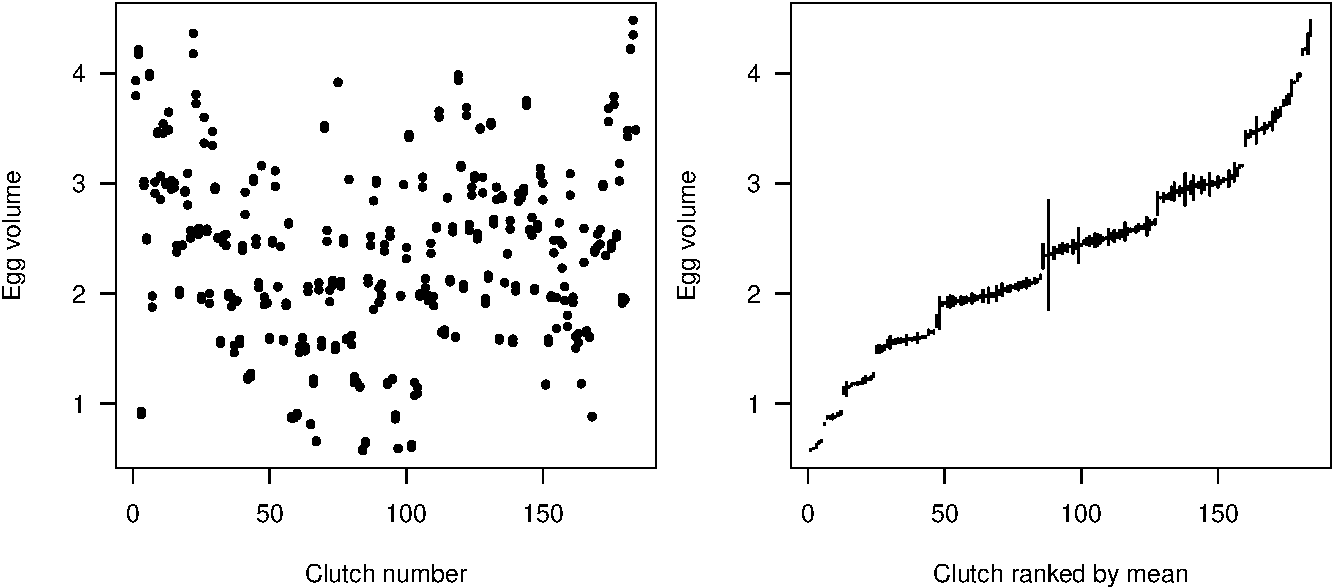
\includegraphics[width=0.95\linewidth,height=\textheight,keepaspectratio]{cluster_files/figure-pdf/fig-coots-volume-1.pdf}

}

\caption{\label{fig-coots-volume}Egg volumes of the American coot. Left:
the two measured eggs of each clutch against the clutch number. Right:
clutches ranked by their mean volume, with the two eggs of each clutch
joined by a segment.}

\end{figure}%

We apply the same ratio estimator, with the estimated clutch totals
\(\hat t_i = M_i\bar y_i\):

\begin{Shaded}
\begin{Highlighting}[]
\NormalTok{coots\_res }\OtherTok{\textless{}{-}} \FunctionTok{cluster\_ratio}\NormalTok{(}\AttributeTok{data =}\NormalTok{ coots,}
                           \AttributeTok{cname =} \StringTok{"clutch"}\NormalTok{,}
                           \AttributeTok{csize =} \StringTok{"csize"}\NormalTok{,}
                           \AttributeTok{yvar =} \StringTok{"volume"}\NormalTok{)}
\NormalTok{coots\_res}\SpecialCharTok{$}\NormalTok{table}
\end{Highlighting}
\end{Shaded}

\begin{table}[H]
\caption*{
{\large  Ratio Estimation: Working Table\normalsize } \\ 
{\normalsize  \(n = 184\)\normalsize }
} 
\normalsize
\begin{gtfit}{\linewidth}{>{\raggedright\arraybackslash}p{\dimexpr 30.00pt -2\tabcolsep-1.5\arrayrulewidth}>{\raggedleft\arraybackslash}p{\dimexpr 75.00pt -2\tabcolsep-1.5\arrayrulewidth}>{\raggedleft\arraybackslash}p{\dimexpr 75.00pt -2\tabcolsep-1.5\arrayrulewidth}>{\raggedleft\arraybackslash}p{\dimexpr 75.00pt -2\tabcolsep-1.5\arrayrulewidth}>{\raggedleft\arraybackslash}p{\dimexpr 75.00pt -2\tabcolsep-1.5\arrayrulewidth}>{\raggedleft\arraybackslash}p{\dimexpr 75.00pt -2\tabcolsep-1.5\arrayrulewidth}>{\raggedleft\arraybackslash}p{\dimexpr 75.00pt -2\tabcolsep-1.5\arrayrulewidth}>{\raggedleft\arraybackslash}p{\dimexpr 75.00pt -2\tabcolsep-1.5\arrayrulewidth}}
\toprule
\(i\) & \(m_i\) & \(\bar y_i\) & \(\hat t_i\)\textsuperscript{\textit{1}} & \(M_i\) & \(\hat B M_i\)\textsuperscript{\textit{2}} & \(e_i\) & \(e_i^2\) \\ 
\midrule\addlinespace[2.5pt]
1 & 2.00 & 3.86 & 50.24 & 13.00 & 32.38 & 17.86 & 318.92 \\ 
2 & 2.00 & 4.19 & 54.52 & 13.00 & 32.38 & 22.15 & 490.48 \\ 
3 & 2.00 & 0.92 & 5.50 & 6.00 & 14.94 & -9.45 & 89.23 \\ 
4 & 2.00 & 3.00 & 32.98 & 11.00 & 27.40 & 5.59 & 31.20 \\ 
5 & 2.00 & 2.50 & 24.96 & 10.00 & 24.91 & 0.05 & 0.00 \\ 
6 & 2.00 & 3.98 & 51.80 & 13.00 & 32.38 & 19.42 & 377.05 \\ 
... & ... & ... & ... & ... & ... & ... & ... \\ 
{\bfseries Sum} & {\bfseries 368.00} & {\bfseries ...} & {\bfseries 4,375.95} & {\bfseries 1,757.00} & {\bfseries 4,375.95} & {\bfseries 0.00} & {\bfseries 11,439.58} \\ 
\bottomrule
\end{gtfit}
\begin{minipage}{\linewidth}
\vspace{.05em}
\textsuperscript{\textit{1}}\(\hat t_i = \bar y_i \, M_i\).\\
\textsuperscript{\textit{2}}\(\hat B = \sum_i \hat t_i / \sum_i M_i = 2.49\), \(\hat B M_i = \hat B\, M_i\), \(s_e^2 = 62.51\).\\
\(\bar y_r = \dfrac{\sum_i \hat t_i}{\sum_i M_i} = \dfrac{4,375.95}{1,757.00} = 2.49\)\\
\(\mathrm{SE}(\bar y_r) = \dfrac{1}{\bar x}\sqrt{\dfrac{s_e^2}{n}} = \dfrac{1}{9.55}\sqrt{\dfrac{62.51}{184}} = 0.06\)\\
\end{minipage}
\end{table}

Only a subset of eggs is measured in each clutch, so the working table
carries an \(m_i\) column. The function estimates the total volume of
each clutch by multiplying the clutch size \(M_i\) by the mean
\(\bar y_i\) of the measured eggs. The total number of clutches \(N\) is
unknown but presumably very large, so the psu-level fpc is
\(1 - n/N \approx 1\) and the within-clutch term, with its factor
\(1/(nN)\), is negligible. No within-cluster variance column appears:
with \texttt{N\ =\ Inf}, \(s_e^2\) carries all of the subsampling noise
on its own.

\begin{Shaded}
\begin{Highlighting}[]
\NormalTok{coots\_res}\SpecialCharTok{$}\NormalTok{estimate }\SpecialCharTok{|\textgreater{}} \FunctionTok{format\_est\_gt}\NormalTok{(}\StringTok{"ratio\_mean"}\NormalTok{)}
\end{Highlighting}
\end{Shaded}

\begin{table}[H]
\normalsize
\begin{gtfit}{0.7\linewidth}{rrrr}
\toprule
\(\bar{y}_{r}\) & \(\mathrm{SE}(\bar{y}_{r})\) & 95\% CI Lower & 95\% CI Upper \\ 
\midrule\addlinespace[2.5pt]
2.49 & 0.06 & 2.37 & 2.61 \\ 
\bottomrule
\end{gtfit}
\end{table}

The estimated mean egg volume is 2.491, with standard error 0.061, a
coefficient of variation of only 0.0245.

\subsection{Example: farm acreage, with states as clusters
(agpop.csv)}\label{sec-cluster-agpop}

Neither example above actually exercises the within-cluster term:
\texttt{algebra} is one-stage, and \texttt{coots} has an unknown \(N\).
To see it at work we need a population whose clusters we can count. The
\texttt{agpop.csv} file provides one: its 3,059 counties (dropping those
coded \texttt{-99}) sit inside exactly \(N = 50\) states, so the states
are clusters of known number and known sizes \(M_i\).

\subsubsection*{Drawing the sample}\label{drawing-the-sample}
\addcontentsline{toc}{subsubsection}{Drawing the sample}

We take a two-stage sample: an SRS of \(n = 10\) states, followed by an
SRS of \(m_i \approx 30\%\) of the counties in each selected state.

\begin{Shaded}
\begin{Highlighting}[]
\NormalTok{agpop }\OtherTok{\textless{}{-}} \FunctionTok{acres\_in\_thousands}\NormalTok{(}\FunctionTok{read.csv}\NormalTok{(}\StringTok{"data/agpop.csv"}\NormalTok{))}
\NormalTok{agpop }\OtherTok{\textless{}{-}}\NormalTok{ agpop[}\SpecialCharTok{!}\FunctionTok{is.na}\NormalTok{(agpop}\SpecialCharTok{$}\NormalTok{acres92), ]}

\DocumentationTok{\#\# cluster sizes M\_i: the number of counties in each state}
\NormalTok{Mi\_all }\OtherTok{\textless{}{-}} \FunctionTok{table}\NormalTok{(agpop}\SpecialCharTok{$}\NormalTok{state)}
\NormalTok{agpop}\SpecialCharTok{$}\NormalTok{Mi }\OtherTok{\textless{}{-}} \FunctionTok{as.integer}\NormalTok{(Mi\_all[agpop}\SpecialCharTok{$}\NormalTok{state])}

\FunctionTok{set.seed}\NormalTok{(}\DecValTok{2026}\NormalTok{)}
\NormalTok{states }\OtherTok{\textless{}{-}} \FunctionTok{sample}\NormalTok{(}\FunctionTok{names}\NormalTok{(Mi\_all), }\DecValTok{10}\NormalTok{)                 }\CommentTok{\# stage 1: n = 10 clusters}
\NormalTok{agclus }\OtherTok{\textless{}{-}} \FunctionTok{do.call}\NormalTok{(rbind, }\FunctionTok{lapply}\NormalTok{(states, }\ControlFlowTok{function}\NormalTok{(st) \{}
\NormalTok{  rows }\OtherTok{\textless{}{-}} \FunctionTok{which}\NormalTok{(agpop}\SpecialCharTok{$}\NormalTok{state }\SpecialCharTok{==}\NormalTok{ st)                  }\CommentTok{\# stage 2: m\_i = 0.3 M\_i}
\NormalTok{  agpop[}\FunctionTok{sample}\NormalTok{(rows, }\FunctionTok{max}\NormalTok{(}\DecValTok{1}\NormalTok{, }\FunctionTok{round}\NormalTok{(}\FloatTok{0.30} \SpecialCharTok{*} \FunctionTok{length}\NormalTok{(rows)))), ]}
\NormalTok{\}))}

\FunctionTok{c}\NormalTok{(}\AttributeTok{clusters =} \FunctionTok{length}\NormalTok{(states), }\AttributeTok{counties =} \FunctionTok{nrow}\NormalTok{(agclus))}
\end{Highlighting}
\end{Shaded}

\begin{verbatim}
clusters counties 
      10      184 
\end{verbatim}

\subsubsection*{Computing the estimate
directly}\label{computing-the-estimate-directly}
\addcontentsline{toc}{subsubsection}{Computing the estimate directly}

Everything the estimator needs is a cluster-level summary: the known
size \(M_i\) of each sampled state, the number of counties actually
measured in it (\(m_i\)), their mean \(\bar{y}_i\) and variance
\(s_i^2\), and the estimated state total \(\hat{t}_i = M_i \bar{y}_i\).

\begin{Shaded}
\begin{Highlighting}[]
\NormalTok{n  }\OtherTok{\textless{}{-}} \FunctionTok{length}\NormalTok{(states)                                            }\CommentTok{\# clusters drawn}
\NormalTok{N  }\OtherTok{\textless{}{-}} \DecValTok{50}                                                        \CommentTok{\# clusters in all}

\NormalTok{Mi    }\OtherTok{\textless{}{-}} \FunctionTok{tapply}\NormalTok{(agclus}\SpecialCharTok{$}\NormalTok{Mi,      agclus}\SpecialCharTok{$}\NormalTok{state, }\ControlFlowTok{function}\NormalTok{(x) x[}\DecValTok{1}\NormalTok{])  }\CommentTok{\# cluster sizes}
\NormalTok{mi    }\OtherTok{\textless{}{-}} \FunctionTok{tapply}\NormalTok{(agclus}\SpecialCharTok{$}\NormalTok{acres92, agclus}\SpecialCharTok{$}\NormalTok{state, length)            }\CommentTok{\# counties measured}
\NormalTok{ybari }\OtherTok{\textless{}{-}} \FunctionTok{tapply}\NormalTok{(agclus}\SpecialCharTok{$}\NormalTok{acres92, agclus}\SpecialCharTok{$}\NormalTok{state, mean)              }\CommentTok{\# subsample means}
\NormalTok{si2   }\OtherTok{\textless{}{-}} \FunctionTok{tapply}\NormalTok{(agclus}\SpecialCharTok{$}\NormalTok{acres92, agclus}\SpecialCharTok{$}\NormalTok{state, var)               }\CommentTok{\# within{-}cluster vars}
\NormalTok{thati }\OtherTok{\textless{}{-}}\NormalTok{ Mi }\SpecialCharTok{*}\NormalTok{ ybari                                              }\CommentTok{\# estimated totals}

\NormalTok{clus\_summary }\OtherTok{\textless{}{-}} \FunctionTok{data.frame}\NormalTok{(Mi, mi, ybari, si2, thati)}

\NormalTok{clus\_summary }\SpecialCharTok{|\textgreater{}}
  \FunctionTok{gt}\NormalTok{(}\AttributeTok{rownames\_to\_stub =} \ConstantTok{TRUE}\NormalTok{) }\SpecialCharTok{|\textgreater{}}
  \FunctionTok{cols\_label}\NormalTok{(}\AttributeTok{Mi    =} \FunctionTok{md}\NormalTok{(}\StringTok{"$M\_i$"}\NormalTok{),    }\AttributeTok{mi  =} \FunctionTok{md}\NormalTok{(}\StringTok{"$m\_i$"}\NormalTok{),}
             \AttributeTok{ybari =} \FunctionTok{md}\NormalTok{(}\StringTok{"$}\SpecialCharTok{\textbackslash{}\textbackslash{}}\StringTok{bar y\_i$"}\NormalTok{), }\AttributeTok{si2 =} \FunctionTok{md}\NormalTok{(}\StringTok{"$s\_i\^{}2$"}\NormalTok{),}
             \AttributeTok{thati =} \FunctionTok{md}\NormalTok{(}\StringTok{"$}\SpecialCharTok{\textbackslash{}\textbackslash{}}\StringTok{hat t\_i$"}\NormalTok{)) }\SpecialCharTok{|\textgreater{}}
  \FunctionTok{fmt\_auto}\NormalTok{(}\AttributeTok{data =}\NormalTok{ clus\_summary, }\AttributeTok{columns =} \FunctionTok{c}\NormalTok{(}\StringTok{"ybari"}\NormalTok{, }\StringTok{"si2"}\NormalTok{, }\StringTok{"thati"}\NormalTok{))}
\end{Highlighting}
\end{Shaded}

\begin{table}

\caption{\label{tbl-agpop-cluster-summary}Cluster-level summaries for
the 10 sampled states}

\centering{

\normalsize
\begin{gtfit}{\linewidth}{l|rrrrr}
\toprule
 & \(M_i\) & \(m_i\) & \(\bar y_i\) & \(s_i^2\) & \(\hat t_i\) \\ 
\midrule\addlinespace[2.5pt]
CA & 58 & 17 & 443.89 & 203,331.78 & 25,745.46 \\ 
NC & 100 & 30 & 90.67 & 3,996.75 & 9,066.94 \\ 
NE & 93 & 28 & 489.72 & 100,362.46 & 45,543.98 \\ 
NJ & 21 & 6 & 40.47 & 2,483.35 & 849.86 \\ 
NV & 15 & 4 & 213.67 & 41,391.58 & 3,204.99 \\ 
NY & 59 & 18 & 123.28 & 9,047.88 & 7,273.64 \\ 
OK & 77 & 23 & 395.78 & 21,374.08 & 30,475.10 \\ 
PA & 65 & 20 & 104.15 & 5,516.48 & 6,769.90 \\ 
UT & 29 & 9 & 396.64 & 130,980.12 & 11,502.66 \\ 
VA & 96 & 29 & 67.00 & 2,568.08 & 6,431.95 \\ 
\bottomrule
\end{gtfit}

}

\end{table}%

The states drawn range from 15 to 100 counties, of which 4 to 30 were
visited. \(s_i^2\) is large throughout: county acreages vary enormously
even inside a single state, and that is the variability the second-stage
term accounts for.

The ratio estimate divides the estimated totals by the cluster sizes:

\begin{Shaded}
\begin{Highlighting}[]
\NormalTok{Mbar  }\OtherTok{\textless{}{-}} \FunctionTok{mean}\NormalTok{(Mi)                  }\CommentTok{\# average size of the sampled clusters}
\NormalTok{ybarr }\OtherTok{\textless{}{-}} \FunctionTok{sum}\NormalTok{(thati) }\SpecialCharTok{/} \FunctionTok{sum}\NormalTok{(Mi)      }\CommentTok{\# ybar\_r = sum(t\_i hat) / sum(M\_i)}

\FunctionTok{c}\NormalTok{(}\AttributeTok{Mbar =}\NormalTok{ Mbar, }\AttributeTok{ybar\_r =}\NormalTok{ ybarr)}
\end{Highlighting}
\end{Shaded}

\begin{verbatim}
    Mbar   ybar_r 
 61.3000 239.5832 
\end{verbatim}

Its variance has the two pieces from the formula above. The
\textbf{ratio} piece measures how the estimated totals scatter about the
fitted line \(\hat{\bar{y}}_r M_i\):

\begin{Shaded}
\begin{Highlighting}[]
\DocumentationTok{\#\# ratio piece: the variance of the ratio estimate over the 10 sampled states}
\NormalTok{ei  }\OtherTok{\textless{}{-}}\NormalTok{ thati }\SpecialCharTok{{-}}\NormalTok{ ybarr }\SpecialCharTok{*}\NormalTok{ Mi          }\CommentTok{\# ratio residuals}
\NormalTok{se2 }\OtherTok{\textless{}{-}} \FunctionTok{sum}\NormalTok{(ei}\SpecialCharTok{\^{}}\DecValTok{2}\NormalTok{) }\SpecialCharTok{/}\NormalTok{ (n }\SpecialCharTok{{-}} \DecValTok{1}\NormalTok{)         }\CommentTok{\# s\_e\^{}2}
\NormalTok{V\_ratio }\OtherTok{\textless{}{-}}\NormalTok{ (}\DecValTok{1} \SpecialCharTok{{-}}\NormalTok{ n }\SpecialCharTok{/}\NormalTok{ N) }\SpecialCharTok{*}\NormalTok{ se2 }\SpecialCharTok{/}\NormalTok{ (n }\SpecialCharTok{*}\NormalTok{ Mbar}\SpecialCharTok{\^{}}\DecValTok{2}\NormalTok{)}

\FunctionTok{c}\NormalTok{(}\AttributeTok{s\_e2 =}\NormalTok{ se2, }\AttributeTok{V\_ratio =}\NormalTok{ V\_ratio)}
\end{Highlighting}
\end{Shaded}

\begin{verbatim}
        s_e2      V_ratio 
1.650481e+08 3.513821e+03 
\end{verbatim}

The \textbf{stratified} piece treats those same 10 states as strata, of
sizes \(M_i\) inside the \(M = \sum_i M_i\) counties they contain, and
is then scaled by the cluster sampling fraction \(n/N\):

\begin{Shaded}
\begin{Highlighting}[]
\DocumentationTok{\#\# stratified piece: strata = the sampled states, weights W\_i = M\_i / M}
\NormalTok{M     }\OtherTok{\textless{}{-}} \FunctionTok{sum}\NormalTok{(Mi)                                  }\CommentTok{\# elements in the 10 states}
\NormalTok{vi    }\OtherTok{\textless{}{-}}\NormalTok{ (Mi }\SpecialCharTok{/}\NormalTok{ M)}\SpecialCharTok{\^{}}\DecValTok{2} \SpecialCharTok{*}\NormalTok{ (}\DecValTok{1} \SpecialCharTok{{-}}\NormalTok{ mi }\SpecialCharTok{/}\NormalTok{ Mi) }\SpecialCharTok{*}\NormalTok{ si2 }\SpecialCharTok{/}\NormalTok{ mi    }\CommentTok{\# each stratum\textquotesingle{}s contribution}
\NormalTok{V\_str }\OtherTok{\textless{}{-}} \FunctionTok{sum}\NormalTok{(vi)                                  }\CommentTok{\# the stratified variance}

\FunctionTok{c}\NormalTok{(}\AttributeTok{M =}\NormalTok{ M, }\AttributeTok{n\_Mbar =}\NormalTok{ n }\SpecialCharTok{*}\NormalTok{ Mbar, }\AttributeTok{V\_str =}\NormalTok{ V\_str, }\AttributeTok{scaled =}\NormalTok{ (n }\SpecialCharTok{/}\NormalTok{ N) }\SpecialCharTok{*}\NormalTok{ V\_str)}
\end{Highlighting}
\end{Shaded}

\begin{verbatim}
        M    n_Mbar     V_str    scaled 
613.00000 613.00000 180.37073  36.07415 
\end{verbatim}

Adding the two gives the standard error, and the interval uses \(n - 1\)
degrees of freedom, since the clusters, not the counties, are the units
that were randomized.

\begin{Shaded}
\begin{Highlighting}[]
\NormalTok{SE  }\OtherTok{\textless{}{-}} \FunctionTok{sqrt}\NormalTok{(V\_ratio }\SpecialCharTok{+}\NormalTok{ (n }\SpecialCharTok{/}\NormalTok{ N) }\SpecialCharTok{*}\NormalTok{ V\_str)}
\NormalTok{mem }\OtherTok{\textless{}{-}} \FunctionTok{qt}\NormalTok{(}\FloatTok{0.975}\NormalTok{, }\AttributeTok{df =}\NormalTok{ n }\SpecialCharTok{{-}} \DecValTok{1}\NormalTok{) }\SpecialCharTok{*}\NormalTok{ SE}

\FunctionTok{c}\NormalTok{(}\AttributeTok{Est. =}\NormalTok{ ybarr, }\AttributeTok{S.E. =}\NormalTok{ SE, }\AttributeTok{ci.low =}\NormalTok{ ybarr }\SpecialCharTok{{-}}\NormalTok{ mem, }\AttributeTok{ci.upp =}\NormalTok{ ybarr }\SpecialCharTok{+}\NormalTok{ mem)}
\end{Highlighting}
\end{Shaded}

\begin{verbatim}
     Est.      S.E.    ci.low    ci.upp 
239.58317  59.58099 104.80160 374.36475 
\end{verbatim}

The estimated mean 1992 acreage per county is 239.6 thousand acres, with
a 95\% confidence interval of {[}104.8, 374.4{]} thousand acres. The
stratified piece contributes 1\% of the variance; almost all of it comes
from the differences between the states. The interval is wide: only 10
states were visited, so \(n - 1 = 9\) degrees of freedom is all the
between-cluster scatter provides.

\subsubsection*{\texorpdfstring{Using the function
\texttt{cluster\_ratio}}{Using the function cluster\_ratio}}\label{using-the-function-cluster_ratio}
\addcontentsline{toc}{subsubsection}{Using the function
\texttt{cluster\_ratio}}

The function performs exactly these steps, provided \(N\) is supplied.

\begin{Shaded}
\begin{Highlighting}[]
\NormalTok{clus\_res }\OtherTok{\textless{}{-}} \FunctionTok{cluster\_ratio}\NormalTok{(}\AttributeTok{data =}\NormalTok{ agclus,}
                          \AttributeTok{cname =} \StringTok{"state"}\NormalTok{,}
                          \AttributeTok{csize =} \StringTok{"Mi"}\NormalTok{,}
                          \AttributeTok{yvar =} \StringTok{"acres92"}\NormalTok{,}
                          \AttributeTok{N =} \DecValTok{50}\NormalTok{)}

\NormalTok{clus\_res}\SpecialCharTok{$}\NormalTok{table}
\end{Highlighting}
\end{Shaded}

\begin{table}[H]
\caption*{
{\large  Ratio Estimation: Working Table\normalsize } \\ 
{\normalsize  \(n = 10\)\normalsize }
} 
\normalsize
\begin{gtfit}{\linewidth}{>{\raggedright\arraybackslash}p{\dimexpr 30.00pt -2\tabcolsep-1.5\arrayrulewidth}>{\raggedleft\arraybackslash}p{\dimexpr 75.00pt -2\tabcolsep-1.5\arrayrulewidth}>{\raggedleft\arraybackslash}p{\dimexpr 75.00pt -2\tabcolsep-1.5\arrayrulewidth}>{\raggedleft\arraybackslash}p{\dimexpr 75.00pt -2\tabcolsep-1.5\arrayrulewidth}>{\raggedleft\arraybackslash}p{\dimexpr 75.00pt -2\tabcolsep-1.5\arrayrulewidth}>{\raggedleft\arraybackslash}p{\dimexpr 75.00pt -2\tabcolsep-1.5\arrayrulewidth}>{\raggedleft\arraybackslash}p{\dimexpr 75.00pt -2\tabcolsep-1.5\arrayrulewidth}>{\raggedleft\arraybackslash}p{\dimexpr 75.00pt -2\tabcolsep-1.5\arrayrulewidth}>{\raggedleft\arraybackslash}p{\dimexpr 75.00pt -2\tabcolsep-1.5\arrayrulewidth}>{\raggedleft\arraybackslash}p{\dimexpr 75.00pt -2\tabcolsep-1.5\arrayrulewidth}}
\toprule
\(i\) & \(m_i\) & \(\bar y_i\) & \(s_i^2\) & \(\hat t_i\)\textsuperscript{\textit{1}} & \(M_i\) & \(\hat B M_i\)\textsuperscript{\textit{2}} & \(e_i\) & \(e_i^2\) & \(\hat v_i\)\textsuperscript{\textit{3}} \\ 
\midrule\addlinespace[2.5pt]
1 & 17.00 & 443.89 & 203,331.78 & 25,745.46 & 58.00 & 13,895.82 & 11,849.63 & 1.40 $\times$ 10\textsuperscript{8} & 75.69 \\ 
2 & 30.00 & 90.67 & 3,996.75 & 9,066.94 & 100.00 & 23,958.32 & -14,891.37 & 2.22 $\times$ 10\textsuperscript{8} & 2.48 \\ 
3 & 28.00 & 489.72 & 100,362.46 & 45,543.98 & 93.00 & 22,281.23 & 23,262.75 & 5.41 $\times$ 10\textsuperscript{8} & 57.66 \\ 
4 & 6.00 & 40.47 & 2,483.35 & 849.86 & 21.00 & 5,031.25 & -4,181.39 & 1.75 $\times$ 10\textsuperscript{7} & 0.35 \\ 
5 & 4.00 & 213.67 & 41,391.58 & 3,204.99 & 15.00 & 3,593.75 & -388.75 & 1.51 $\times$ 10\textsuperscript{5} & 4.54 \\ 
6 & 18.00 & 123.28 & 9,047.88 & 7,273.64 & 59.00 & 14,135.41 & -6,861.77 & 4.71 $\times$ 10\textsuperscript{7} & 3.24 \\ 
... & ... & ... & ... & ... & ... & ... & ... & ... & ... \\ 
{\bfseries Sum} & {\bfseries 184.00} & {\bfseries ...} & {\bfseries ...} & {\bfseries 146,864.48} & {\bfseries 613.00} & {\bfseries 146,864.48} & {\bfseries 0.00} & {\bfseries 1.49 $\times$ 10\textsuperscript{9}} & {\bfseries 180.37} \\ 
\bottomrule
\end{gtfit}
\begin{minipage}{\linewidth}
\vspace{.05em}
\textsuperscript{\textit{1}}\(\hat t_i = \bar y_i \, M_i\).\\
\textsuperscript{\textit{2}}\(\hat B = \sum_i \hat t_i / \sum_i M_i = 239.58\), \(\hat B M_i = \hat B\, M_i\), \(s_e^2 = 1.65 \times 10^{8}\).\\
\textsuperscript{\textit{3}}\(\hat v_i = \left(\dfrac{M_i}{M}\right)^2\left(1-\dfrac{m_i}{M_i}\right)\dfrac{s_i^2}{m_i},\quad M = \sum_i M_i = n\bar M,\quad \sum_i \hat v_i = \hat V_{\mathrm{str}}\).\\
\(\bar y_r = \dfrac{\sum_i \hat t_i}{\sum_i M_i} = \dfrac{1.47 \times 10^{5}}{613.00} = 239.58\)\\
\(\mathrm{SE}(\bar y_r) = \sqrt{\left(1-\dfrac{n}{N}\right)\dfrac{s_e^2}{n\,\bar M^2} + \dfrac{n}{N}\sum_i \hat v_i} = \sqrt{\left(1-\dfrac{10}{50}\right)\dfrac{1.65 \times 10^{8}}{10 \times 61.30^2} + 36.07} = 59.58\)\\
\end{minipage}
\end{table}

Because this sample is two-stage \emph{and} \(N\) is finite, the working
table carries the three extra columns computed above: \(m_i\), the
number of counties measured in each state; \(s_i^2\), the variance among
them; and \(\hat v_i = (M_i/M)^2 (1 - m_i/M_i) s_i^2/m_i\), that state's
contribution to the stratified variance. The Sum of the \(\hat v_i\)
column is \(\hat{V}_{\mathrm{str}}\) itself, and the note under the
table spells the standard error out as
\(\hat{V}_{\mathrm{ratio}} + (n/N)\hat{V}_{\mathrm{str}}\).

\begin{Shaded}
\begin{Highlighting}[]
\NormalTok{clus\_res}\SpecialCharTok{$}\NormalTok{estimate }\SpecialCharTok{|\textgreater{}} \FunctionTok{format\_est\_gt}\NormalTok{(}\StringTok{"ratio\_mean"}\NormalTok{)}
\end{Highlighting}
\end{Shaded}

\begin{table}[H]
\normalsize
\begin{gtfit}{0.7\linewidth}{rrrr}
\toprule
\(\bar{y}_{r}\) & \(\mathrm{SE}(\bar{y}_{r})\) & 95\% CI Lower & 95\% CI Upper \\ 
\midrule\addlinespace[2.5pt]
239.58 & 59.58 & 104.80 & 374.36 \\ 
\bottomrule
\end{gtfit}
\end{table}

The estimate, standard error and interval reproduce the direct
computation above.

\section{Interactive Demonstration: Clustering by State or at
Random}\label{sec-app-cluster}

The simulation for this section runs as a standalone app:
\href{../shinylives_sampling/app-cluster.html}{Two-Stage Cluster
Sampling (ratio estimator) with SRS}. It opens in a new tab, together
with its documentation and the full
\href{../shinylives_sampling/index.html}{list of apps}.

\bookmarksetup{startatroot}

\chapter{Unequal Probability
Sampling}\label{unequal-probability-sampling}

Unequal probability sampling (UPS) selects units with different
probabilities, usually in proportion to a \textbf{size variable} known
for every unit in the population. Large units contribute more to a
total, so we give them a larger chance of being selected, and correct
for this in the estimator. This chapter builds UPS in three steps, each
a special case or an extension of the previous one:

\begin{enumerate}
\def\labelenumi{\arabic{enumi}.}
\tightlist
\item
  \textbf{The Hansen--Hurwitz (HH) estimator}: the selection
  probabilities \(\psi_i\) are built from an auxiliary variable \(x_i\),
  and we estimate the total or mean of \(y_i\)
  (Section~\ref{sec-ups-hh}).
\item
  \textbf{One-stage cluster sampling}: the units are clusters (psus),
  \(y_i\) is the cluster total \(t_i\), and \(x_i\) is the cluster size
  \(M_i\) (Section~\ref{sec-ups-cluster}).
\item
  \textbf{Two-stage cluster sampling}: the cluster total \(t_i\) is not
  observed, but estimated from a subsample of the cluster
  (Section~\ref{sec-ups-twostage}).
\end{enumerate}

Sampling \textbf{with replacement} (UPSWR) is used throughout, since it
makes the variance easy to estimate: we make \(n\) independent draws,
and on each draw unit \(i\) is selected with probability \(\psi_i\),
where \(\sum_{i=1}^N\psi_i=1\). A unit may be selected more than once,
and it then appears in the sample once per draw. Sampling without
replacement is briefly discussed at the end (Section~\ref{sec-ups-wo}).

\section{Functions and Packages}\label{functions-and-packages}

The estimating functions used throughout this book (in this chapter
\texttt{upswr\_est} and \texttt{upswr\_total} for sampling with
replacement, \texttt{upswo\_est} for sampling without replacement,
\texttt{srs\_est}, \texttt{ratio\_est} and \texttt{reg\_est} for
comparison, and the \texttt{format\_est\_gt} table-formatting helper)
live in a single shared file, \texttt{samplingestimate.r}, which we
source below.

The full source of \texttt{samplingestimate.r} is listed in
Appendix~\ref{sec-estimating-functions}.

\section{The Hansen--Hurwitz Estimator}\label{sec-ups-hh}

\subsection{Theory}\label{sec-ups-hh-theory}

The population has \(N\) units. Unit \(i\) has a study value \(y_i\),
with population total \(t=\sum_{i=1}^N y_i\) and mean \(\bar{y}_U=t/N\),
and an auxiliary variable \(x_i>0\) whose total \(t_x=\sum_{i=1}^N x_i\)
is known. If \(y_i\) is roughly proportional to \(x_i\) (for example,
the number of physicians of a county and its population), we construct
the selection probabilities from \(x_i\): \[
\psi_i=\frac{x_i}{t_x}.
\]

\textbf{The ratio of each unit.} Define, for every unit of the
population, \[
b_i=\frac{y_i}{x_i},\qquad i=1,\ldots,N,
\] and let \(B=t/t_x=\bar{y}_U/\bar{x}_U\) be the population ratio.
Since \(y_i=x_ib_i\), \(B\) is the mean of the \(b_i\) weighted by
\(x_i\), \[
B=\frac{\sum_{i=1}^N x_ib_i}{\sum_{i=1}^N x_i},
\] and once \(B\) is known, the mean and the total follow, \[
\bar{y}_U=\bar{x}_U\,B,\qquad t=t_x\,B,\qquad \bar{x}_U=\frac{t_x}{N}.
\] So estimating \(B\) is enough: we build an estimator \(\hat{B}\) and
convert it to \(\hat{\bar{y}}=\bar{x}_U\hat{B}\) and
\(\hat{t}=t_x\hat{B}\). Everything below, for HH, the ratio estimator
and the sample average, is written in terms of the \(b_i\).

\textbf{The sample \(\mathcal{R}\) and its observations \(b_j^*\).} We
make \(n\) independent draws with replacement; on each draw, unit \(i\)
is selected with probability \(\psi_i=x_i/t_x\). The sample, denoted
\(\mathcal{R}\) (not \(\mathcal{S}\)), is the list of the \(n\) draws
\textbf{including repeats}: a unit drawn twice appears twice. Let
\(b_j^*\) denote the ratio \(b\) of the unit selected on the \(j\)th
draw, that is, the \(j\)th observation in \(\mathcal{R}\)
(\(j=1,\ldots,n\)). The star reminds us that \(b_j^*\) is indexed by the
draw, not by the population unit: \(b_j^*\) is random, while
\(b_1,\ldots,b_N\) are fixed numbers.

\textbf{Sampling distribution of \(b_j^*\).} On every draw, \(b_j^*\)
equals \(b_i\) exactly when unit \(i\) is selected, so \(b_j^*\) is a
discrete random variable with distribution

{\def\LTcaptype{none} % do not increment counter
\begin{longtable}[]{@{}
  >{\raggedright\arraybackslash}p{(\linewidth - 8\tabcolsep) * \real{0.1667}}
  >{\centering\arraybackslash}p{(\linewidth - 8\tabcolsep) * \real{0.2083}}
  >{\centering\arraybackslash}p{(\linewidth - 8\tabcolsep) * \real{0.2083}}
  >{\centering\arraybackslash}p{(\linewidth - 8\tabcolsep) * \real{0.2083}}
  >{\centering\arraybackslash}p{(\linewidth - 8\tabcolsep) * \real{0.2083}}@{}}
\toprule\noalign{}
\begin{minipage}[b]{\linewidth}\raggedright
Unit selected on draw \(j\)
\end{minipage} & \begin{minipage}[b]{\linewidth}\centering
\(1\)
\end{minipage} & \begin{minipage}[b]{\linewidth}\centering
\(2\)
\end{minipage} & \begin{minipage}[b]{\linewidth}\centering
\(\cdots\)
\end{minipage} & \begin{minipage}[b]{\linewidth}\centering
\(N\)
\end{minipage} \\
\midrule\noalign{}
\endhead
\bottomrule\noalign{}
\endlastfoot
Value of \(b_j^*\) & \(b_1\) & \(b_2\) & \(\cdots\) & \(b_N\) \\
Probability & \(\psi_1=x_1/t_x\) & \(\psi_2=x_2/t_x\) & \(\cdots\) &
\(\psi_N=x_N/t_x\) \\
\end{longtable}
}

(if several units have the same value of \(b_i\), their probabilities
add up). Since the draws are made with replacement, the probabilities do
not change from draw to draw, and \(b_1^*,\ldots,b_n^*\) are
\textbf{independent and identically distributed} (iid) with this
distribution. Its mean and variance are \[
E(b_j^*)=\sum_{i=1}^N\frac{x_i}{t_x}\cdot\frac{y_i}{x_i}=\frac{t}{t_x}=B,\qquad
S_{b^*}^2=V(b_j^*)=\sum_{i=1}^N\psi_i\,(b_i-B)^2 .
\] A single draw is therefore an unbiased estimate of \(B\), and it is a
precise one when the \(b_i\) are nearly the same for all units, that is,
when \(y_i\) is nearly proportional to \(x_i\).

\textbf{Hansen--Hurwitz estimator of \(B\).} The HH estimator is the
average of the \(n\) observations in \(\mathcal{R}\), the \textbf{mean
of the ratios}: \[
\boxed{\hat{B}_{\mathrm{HH}}=\bar{b}^*=\frac{1}{n}\sum_{j=1}^n b_j^*} .
\] Being the mean of \(n\) iid copies of \(b_j^*\), it is unbiased, and
its variance is that of one draw divided by \(n\): \[
E(\hat{B}_{\mathrm{HH}})=B,\qquad
V(\hat{B}_{\mathrm{HH}})=\frac{S_{b^*}^2}{n}=\frac{1}{nN}\sum_{i=1}^N w^x_i\,(b_i-B)^2 ,
\qquad w^x_i=\frac{x_i}{\bar{x}_U}=N\psi_i .
\] Here \(w^x_i\) is the size of unit \(i\) relative to the average, so
that \(\psi_i=w^x_i/N\), and the variance is a sum of terms involving
only \(w^x_i\) and \(b_i-B\). There is no finite population correction,
since the draws are independent. For the same reason, the sample
variance of the \(b_j^*\) is an unbiased estimate of \(S_{b^*}^2\),
which gives \[
\boxed{\widehat{\mathrm{SE}}(\hat{B}_{\mathrm{HH}})=\frac{s_{b^*}}{\sqrt{n}}},\qquad
s_{b^*}^2=\frac{1}{n-1}\sum_{j=1}^n\left(b_j^*-\bar{b}^*\right)^2 .
\]

\textbf{Mean and total.} Multiplying by the known \(\bar{x}_U\) and
\(t_x\), the estimator, its standard error and its estimated standard
error all scale by the same constant: \[
\boxed{\;
\begin{aligned}
\hat{\bar{y}}_{\mathrm{HH}}&=\bar{x}_U\,\hat{B}_{\mathrm{HH}}=\bar{x}_U\,\bar{b}^*,\qquad
&\mathrm{SE}(\hat{\bar{y}}_{\mathrm{HH}})&=\bar{x}_U\,\frac{S_{b^*}}{\sqrt{n}},\qquad
&\widehat{\mathrm{SE}}(\hat{\bar{y}}_{\mathrm{HH}})&=\bar{x}_U\,\frac{s_{b^*}}{\sqrt{n}},\\[4pt]
\hat{t}_{\mathrm{HH}}&=t_x\,\hat{B}_{\mathrm{HH}}=t_x\,\bar{b}^*,\qquad
&\mathrm{SE}(\hat{t}_{\mathrm{HH}})&=t_x\,\frac{S_{b^*}}{\sqrt{n}},\qquad
&\widehat{\mathrm{SE}}(\hat{t}_{\mathrm{HH}})&=t_x\,\frac{s_{b^*}}{\sqrt{n}} .
\end{aligned}\;}
\] In the more general notation of unequal probability sampling,
\(y_j^*/\psi_j^*=t_x\,b_j^*\) is the estimate of the total from draw
\(j\), so \(\hat{t}_{\mathrm{HH}}=\frac1n\sum_{j=1}^n y_j^*/\psi_j^*\).
This form works for any \(\psi_i\), not only for \(\psi_i=x_i/t_x\), and
is what the function \texttt{upswr\_total} computes; for
\(\psi_i=x_i/t_x\), the function \texttt{upswr\_est} works directly with
the ratios \(b_j^*\).

\textbf{Variance of the mean and total.} The variances of
\(\hat{\bar{y}}_{\mathrm{HH}}\) and \(\hat{t}_{\mathrm{HH}}\) are
\(\bar{x}_U^2\) and \(t_x^2\) times \(V(\hat{B}_{\mathrm{HH}})\). The
variance is small when all the ratios \(b_i\) are close to \(B\), that
is, when \(y_i\) is nearly proportional to \(x_i\).

\subsection{\texorpdfstring{Comparison of the HH, Ratio, and Average
Estimators of
\(B\)}{Comparison of the HH, Ratio, and Average Estimators of B}}\label{sec-ups-compare}

The ratio estimator and the sample average are used with a simple random
sample (SRS) \(\mathcal{S}\) of \(n\) units without replacement. Let
\(w^x_i=x_i/\bar{x}_U\) be the size of unit \(i\) relative to the
average, and \(d_i=y_i-Bx_i=x_i(b_i-B)\) the residuals about the line
through the origin \(y=Bx\). Each estimator is also an estimator of
\(B\), which is then multiplied by \(\bar{x}_U\) or \(t_x\).

\begin{itemize}
\item
  The \textbf{ratio estimator} (Section~\ref{sec-ratio-theory})
  estimates \(\bar{y}_U\) by \(\bar{x}_U\,\bar{y}/\bar{x}\). Since
  \(y_i=x_ib_i\), \[
  \hat{B}_r=\frac{\bar{y}}{\bar{x}}=\frac{\sum_{i\in\mathcal{S}}y_i}{\sum_{i\in\mathcal{S}}x_i}
  =\frac{\sum_{i\in\mathcal{S}}x_i\,b_i}{\sum_{i\in\mathcal{S}}x_i},
  \] the mean of the sampled \(b_i\) weighted by \(x_i\) (weights adding
  up to one), and \(\hat{\bar{y}}_r=\bar{x}_U\hat{B}_r\),
  \(\hat{t}_r=t_x\hat{B}_r\).
\item
  The \textbf{sample average} \(\bar{y}\) ignores \(x_i\). Since
  \(y_i=x_ib_i=\bar{x}_U\,w^x_ib_i\), \[
  \bar{y}=\bar{x}_U\cdot\frac{1}{n}\sum_{i\in\mathcal{S}}w^x_i\,b_i
  \quad\Longrightarrow\quad
  \hat{B}_{\mathrm{avg}}=\frac{\bar{y}}{\bar{x}_U}=\frac{1}{n}\sum_{i\in\mathcal{S}}w^x_i\,b_i ,
  \] the mean of the sampled \(b_i\) with weights \(w^x_i\) that do not
  add up to one, and
  \(\hat{t}_{\mathrm{avg}}=t_x\hat{B}_{\mathrm{avg}}\).
\end{itemize}

Table~\ref{tbl-ups-compare} compares them with the HH estimator
\(\hat{B}_{\mathrm{HH}}=\frac1n\sum_{j=1}^n b_j^*\). Their variances
follow from the variances of \(\bar{y}\) and \(\hat{\bar{y}}_r\) for SRS
divided by \(\bar{x}_U^2\), using
\(w^x_ib_i-B=(y_i-\bar{y}_U)/\bar{x}_U\) and
\(w^x_i(b_i-B)=d_i/\bar{x}_U\) (the ratio estimator's variance is the
large-\(n\) approximation), and from the HH variance of the theory
section.

\begin{longtable}[]{@{}
  >{\raggedright\arraybackslash}p{(\linewidth - 8\tabcolsep) * \real{0.2000}}
  >{\centering\arraybackslash}p{(\linewidth - 8\tabcolsep) * \real{0.2000}}
  >{\centering\arraybackslash}p{(\linewidth - 8\tabcolsep) * \real{0.2000}}
  >{\raggedright\arraybackslash}p{(\linewidth - 8\tabcolsep) * \real{0.2000}}
  >{\raggedright\arraybackslash}p{(\linewidth - 8\tabcolsep) * \real{0.2000}}@{}}
\caption{Estimators of \(B=t/t_x\) from SRS and UPSWR samples of \(n\)
units.}\label{tbl-ups-compare}\tabularnewline
\toprule\noalign{}
\begin{minipage}[b]{\linewidth}\raggedright
Estimator
\end{minipage} & \begin{minipage}[b]{\linewidth}\centering
Estimator of \(B\)
\end{minipage} & \begin{minipage}[b]{\linewidth}\centering
Variance
\end{minipage} & \begin{minipage}[b]{\linewidth}\raggedright
\(x_i\) is used at
\end{minipage} & \begin{minipage}[b]{\linewidth}\raggedright
Unbiased?
\end{minipage} \\
\midrule\noalign{}
\endfirsthead
\toprule\noalign{}
\begin{minipage}[b]{\linewidth}\raggedright
Estimator
\end{minipage} & \begin{minipage}[b]{\linewidth}\centering
Estimator of \(B\)
\end{minipage} & \begin{minipage}[b]{\linewidth}\centering
Variance
\end{minipage} & \begin{minipage}[b]{\linewidth}\raggedright
\(x_i\) is used at
\end{minipage} & \begin{minipage}[b]{\linewidth}\raggedright
Unbiased?
\end{minipage} \\
\midrule\noalign{}
\endhead
\bottomrule\noalign{}
\endlastfoot
Sample average (SRS) &
\(\hat{B}_{\mathrm{avg}}=\dfrac1n\sum\limits_{i\in\mathcal{S}}w^x_ib_i\)
&
\(\left(1-\dfrac{n}{N}\right)\dfrac{1}{n(N-1)}\sum\limits_{i=1}^N (w^x_ib_i-B)^2\)
& not used & yes, for \(\bar{y}_U/\bar{x}_U\) \\
Ratio (SRS) &
\(\hat{B}_r=\dfrac{\sum_{i\in\mathcal{S}} x_ib_i}{\sum_{i\in\mathcal{S}} x_i}\)
&
\(\approx\left(1-\dfrac{n}{N}\right)\dfrac{1}{n(N-1)}\sum\limits_{i=1}^N (w^x_i)^2\,(b_i-B)^2\)
& the \textbf{estimation} stage & slightly biased \\
HH (UPSWR, \(\psi_i=x_i/t_x\)) &
\(\hat{B}_{\mathrm{HH}}=\dfrac1n\sum\limits_{j=1}^n b_j^*\) &
\(\dfrac{1}{nN}\sum\limits_{i=1}^N w^x_i\,(b_i-B)^2\) & the
\textbf{design} stage & exactly unbiased \\
\end{longtable}

\emph{Note:} for the sample average, \(w^x_i=x_i/\bar{x}_U\) and
\(w^x_ib_i=y_i/\bar{x}_U\), so that
\(\hat{B}_{\mathrm{avg}}=\bar{y}/\bar{x}_U\) and its variance is the SRS
variance of \(y_i\) divided by \(\bar{x}_U^2\).

For the mean and the total, multiply the estimators by \(\bar{x}_U\) and
\(t_x\), and the variances by \(\bar{x}_U^2\) and \(t_x^2\).

Ignoring the finite population correction and the difference between
\(N-1\) and \(N\), each variance is \(\frac1n\) times an average over
the units of one squared term:

{\def\LTcaptype{none} % do not increment counter
\begin{longtable}[]{@{}
  >{\raggedright\arraybackslash}p{(\linewidth - 4\tabcolsep) * \real{0.3333}}
  >{\raggedright\arraybackslash}p{(\linewidth - 4\tabcolsep) * \real{0.3333}}
  >{\raggedright\arraybackslash}p{(\linewidth - 4\tabcolsep) * \real{0.3333}}@{}}
\toprule\noalign{}
\begin{minipage}[b]{\linewidth}\raggedright
Estimator
\end{minipage} & \begin{minipage}[b]{\linewidth}\raggedright
Squared term of unit \(i\)
\end{minipage} & \begin{minipage}[b]{\linewidth}\raggedright
Spread of \(y\) about
\end{minipage} \\
\midrule\noalign{}
\endhead
\bottomrule\noalign{}
\endlastfoot
Sample average & \((w^x_ib_i-B)^2\) & the flat line \(\bar{y}_U\) \\
Ratio & \((w^x_i)^2\,(b_i-B)^2\) & the line \(y=Bx\) \\
HH & \(w^x_i\,(b_i-B)^2\) & the line \(y=Bx\), with weight \(1/w^x_i\)
relative to the ratio estimator \\
\end{longtable}
}

The ratio estimator and HH use the same ratios and the same centre
\(B\), so their terms differ only in one factor: \((w^x_i)^2\) for the
ratio estimator, \(w^x_i\) for HH. HH multiplies the term of the ratio
estimator by \(1/w^x_i=\bar{x}_U/x_i\). A unit larger than average
(\(w^x_i>1\)) is \textbf{downweighted} under HH, and a smaller one is
upweighted. The reason is that HH gives equal weights to the draws
because the large units are already drawn more often, whereas the ratio
estimator must give the large units larger weights \(x_i\) to compensate
for the equal chances. UPSWR therefore wins when the large residuals
\(d_i\) belong to the large units, that is, when the spread of \(y_i\)
about the line grows with \(x_i\), as it does for county acreages. When
the spread of \(y_i\) is the same for all \(x_i\) (so that
\(b_i-B\propto1/x_i\)), the SRS ratio estimator does better. When
\(y_i\) is not related to \(x_i\) at all, all the \(b_i-B\) are large
and both estimators can be worse than the plain sample average. The next
section illustrates these cases.

\subsection{Toy Example: Four Supermarkets}\label{sec-ups-toy}

A town has four supermarkets, with floor areas \(x_i\) from
\(100\,\text{m}^2\) to \(1000\,\text{m}^2\), so \(t_x=1600\),
\(\bar{x}_U=400\) and \(w^x_i=x_i/\bar{x}_U=0.25,\,0.5,\,0.75,\,2.5\).
We want to estimate the monthly sales per square metre
\(B=\bar{y}_U/\bar{x}_U\), from the ratios \(b_i=y_i/x_i\) of the stores
(the mean and the total of sales follow by multiplying by \(\bar{x}_U\)
and \(t_x\)). The data for the first population (the sales, in thousands
of dollars per month, are nearly proportional to the floor areas) are:

{\def\LTcaptype{none} % do not increment counter
\begin{longtable}[]{@{}
  >{\raggedright\arraybackslash}p{(\linewidth - 6\tabcolsep) * \real{0.3647}}
  >{\raggedleft\arraybackslash}p{(\linewidth - 6\tabcolsep) * \real{0.3059}}
  >{\raggedleft\arraybackslash}p{(\linewidth - 6\tabcolsep) * \real{0.1647}}
  >{\raggedleft\arraybackslash}p{(\linewidth - 6\tabcolsep) * \real{0.1647}}@{}}
\toprule\noalign{}
\begin{minipage}[b]{\linewidth}\raggedright
Store
\end{minipage} & \begin{minipage}[b]{\linewidth}\raggedleft
\(x_i\) (floor area, m\(^2\))
\end{minipage} & \begin{minipage}[b]{\linewidth}\raggedleft
\(y_i\) (sales)
\end{minipage} & \begin{minipage}[b]{\linewidth}\raggedleft
\(b_i=y_i/x_i\)
\end{minipage} \\
\midrule\noalign{}
\endhead
\bottomrule\noalign{}
\endlastfoot
A & 100 & 11 & 0.1100 \\
B & 200 & 20 & 0.1000 \\
C & 300 & 24 & 0.0800 \\
D & 1,000 & 245 & 0.2450 \\
\textbf{Total} & 1,600 & 300 & \\
\textbf{True \(B=\sum y_i/\sum x_i\)} & & & 0.1875 \\
\end{longtable}
}

To compare the three estimators of \(B\) in
Section~\ref{sec-ups-compare}, we work out their variances for a
\textbf{single draw} (\(n=1\)); for \(n\) draws, each is divided by
\(n\). For the two SRS estimators we take \(N=\infty\), that is, we
ignore the finite population correction, so a single draw has the
variance of one value drawn with equal probabilities \(1/N\) (hence the
divisor \(N\) rather than \(N-1\)). The one-draw variance of each
estimator is \(\frac1N\) times the sum over the stores of its squared
term:

{\def\LTcaptype{none} % do not increment counter
\begin{longtable}[]{@{}lll@{}}
\toprule\noalign{}
Estimator & Design & Squared term of store \(i\) \\
\midrule\noalign{}
\endhead
\bottomrule\noalign{}
\endlastfoot
Sample average & SRS & \((w^x_ib_i-B)^2\) \\
Ratio & SRS & \((w^x_i)^2\,(b_i-B)^2\) \\
HH & PPS, \(\psi_i=x_i/t_x\) & \(w^x_i\,(b_i-B)^2\) \\
\end{longtable}
}

For each population below, a single table works out the three variances
side by side. The \textbf{Sum} row adds the squared terms, and the
\textbf{Variance} row divides the sum by \(N\).

\textbf{Sales proportional to floor area.} The monthly sales (thousands
of dollars) are nearly proportional to the floor areas, as in the slides
for this chapter. Here \(t=300\), \(\bar{y}_U=75\) and
\(B=300/1600=0.1875\).

\textbf{HH is unbiased.} With one draw, the HH estimate of \(B\) is
\(b_i\) when store \(i\) is selected, which happens with probability
\(\psi_i\), so \(E(\hat{B}_{\mathrm{HH}})=\sum_i\psi_ib_i\), the sum of
the column \(\psi_ib_i\). Multiplying the estimates by \(\bar{x}_U\) or
\(t_x\) gives the estimates of the mean or the total, and the last row
(the sum of \(\psi_i\) times the column) is their expectation:

{\def\LTcaptype{none} % do not increment counter
\begin{longtable}[]{@{}
  >{\raggedright\arraybackslash}p{(\linewidth - 14\tabcolsep) * \real{0.0851}}
  >{\raggedleft\arraybackslash}p{(\linewidth - 14\tabcolsep) * \real{0.0638}}
  >{\raggedleft\arraybackslash}p{(\linewidth - 14\tabcolsep) * \real{0.0638}}
  >{\raggedleft\arraybackslash}p{(\linewidth - 14\tabcolsep) * \real{0.1809}}
  >{\raggedleft\arraybackslash}p{(\linewidth - 14\tabcolsep) * \real{0.0638}}
  >{\raggedleft\arraybackslash}p{(\linewidth - 14\tabcolsep) * \real{0.1277}}
  >{\raggedleft\arraybackslash}p{(\linewidth - 14\tabcolsep) * \real{0.2340}}
  >{\raggedleft\arraybackslash}p{(\linewidth - 14\tabcolsep) * \real{0.1809}}@{}}
\toprule\noalign{}
\begin{minipage}[b]{\linewidth}\raggedright
Store
\end{minipage} & \begin{minipage}[b]{\linewidth}\raggedleft
\(y_i\)
\end{minipage} & \begin{minipage}[b]{\linewidth}\raggedleft
\(x_i\)
\end{minipage} & \begin{minipage}[b]{\linewidth}\raggedleft
\(\psi_i=x_i/t_x\)
\end{minipage} & \begin{minipage}[b]{\linewidth}\raggedleft
\(b_i\)
\end{minipage} & \begin{minipage}[b]{\linewidth}\raggedleft
\(\psi_ib_i\)
\end{minipage} & \begin{minipage}[b]{\linewidth}\raggedleft
\(\bar{x}_Ub_i\) (mean)
\end{minipage} & \begin{minipage}[b]{\linewidth}\raggedleft
\(t_xb_i\) (total)
\end{minipage} \\
\midrule\noalign{}
\endhead
\bottomrule\noalign{}
\endlastfoot
A & 11 & 100 & 0.0625 & 0.110 & 0.00688 & 44 & 176 \\
B & 20 & 200 & 0.1250 & 0.100 & 0.01250 & 40 & 160 \\
C & 24 & 300 & 0.1875 & 0.080 & 0.01500 & 32 & 128 \\
D & 245 & 1,000 & 0.6250 & 0.245 & 0.15313 & 98 & 392 \\
\textbf{Sum} & 300 & 1,600 & 1.0000 & & 0.18750 & 75 & 300 \\
\end{longtable}
}

The four possible estimates of \(B\), 0.11, 0.1, 0.08, 0.245, are all
different from \(B=0.1875\), but weighted by their selection
probabilities they average to \(E(\hat{B}_{\mathrm{HH}})=0.1875=B\), so
\(E(\hat{\bar{y}}_{\mathrm{HH}})=75=\bar{y}_U\) and
\(E(\hat{t}_{\mathrm{HH}})=300=t\). In general,
\(\sum_i\psi_ib_i=\sum_i\frac{x_i}{t_x}\cdot\frac{y_i}{x_i}=\frac{t}{t_x}=B\).
(The same four values are what the ratio estimator gives under an SRS of
one store, but there each has probability \(1/4\), so its expectation is
0.1338 for \(B\), and it is biased.)

\textbf{Variances.} The working table for the three one-draw variances:

{\def\LTcaptype{none} % do not increment counter
\begin{longtable}[]{@{}
  >{\raggedright\arraybackslash}p{(\linewidth - 16\tabcolsep) * \real{0.1838}}
  >{\raggedleft\arraybackslash}p{(\linewidth - 16\tabcolsep) * \real{0.0441}}
  >{\raggedleft\arraybackslash}p{(\linewidth - 16\tabcolsep) * \real{0.0441}}
  >{\raggedleft\arraybackslash}p{(\linewidth - 16\tabcolsep) * \real{0.1618}}
  >{\raggedleft\arraybackslash}p{(\linewidth - 16\tabcolsep) * \real{0.1029}}
  >{\raggedleft\arraybackslash}p{(\linewidth - 16\tabcolsep) * \real{0.0588}}
  >{\raggedleft\arraybackslash}p{(\linewidth - 16\tabcolsep) * \real{0.1250}}
  >{\raggedleft\arraybackslash}p{(\linewidth - 16\tabcolsep) * \real{0.1544}}
  >{\raggedleft\arraybackslash}p{(\linewidth - 16\tabcolsep) * \real{0.1250}}@{}}
\toprule\noalign{}
\begin{minipage}[b]{\linewidth}\raggedright
Store
\end{minipage} & \begin{minipage}[b]{\linewidth}\raggedleft
\(x_i\)
\end{minipage} & \begin{minipage}[b]{\linewidth}\raggedleft
\(y_i\)
\end{minipage} & \begin{minipage}[b]{\linewidth}\raggedleft
\(w^x_i=x_i/\bar{x}_U\)
\end{minipage} & \begin{minipage}[b]{\linewidth}\raggedleft
\(b_i=y_i/x_i\)
\end{minipage} & \begin{minipage}[b]{\linewidth}\raggedleft
\(b_i-B\)
\end{minipage} & \begin{minipage}[b]{\linewidth}\raggedleft
\((w^x_ib_i-B)^2\)
\end{minipage} & \begin{minipage}[b]{\linewidth}\raggedleft
\((w^x_i)^2(b_i-B)^2\)
\end{minipage} & \begin{minipage}[b]{\linewidth}\raggedleft
\(w^x_i(b_i-B)^2\)
\end{minipage} \\
\midrule\noalign{}
\endhead
\bottomrule\noalign{}
\endlastfoot
A & 100 & 11 & 0.25 & 0.110 & -0.0775 & 0.025600 & 0.000375 &
0.001502 \\
B & 200 & 20 & 0.50 & 0.100 & -0.0875 & 0.018906 & 0.001914 &
0.003828 \\
C & 300 & 24 & 0.75 & 0.080 & -0.1075 & 0.016256 & 0.006500 &
0.008667 \\
D & 1,000 & 245 & 2.50 & 0.245 & 0.0575 & 0.180625 & 0.020664 &
0.008266 \\
\textbf{Sum} & 1,600 & 300 & 4.00 & & & 0.241388 & 0.029454 &
0.022262 \\
\textbf{Variance} (Sum / \(N\)) & & & & & & 0.060347 & 0.007363 &
0.005566 \\
\end{longtable}
}

The sample average ignores the floor areas, and its variance, 0.0603, is
dominated by store D, whose sales are far from \(\bar{y}_U=75\). The
ratio estimator measures each store against the line \(y=Bx\) instead,
that is, it looks at \(b_i-B\), which cuts the variance to 0.00736. HH
uses the same ratios, but the largest term of the ratio estimator, store
D's 0.0207, belongs to the largest store, with \(w_D=2.5\): HH divides
it by \(w_D\), giving 0.00827, and the HH variance drops to 0.00557,
about 9\% of that of the sample average. (Multiplying by
\(\bar{x}_U^2=160{,}000\) gives the variances of the estimates of the
mean, 9,656, 1,178.2 and 890.5.)

\textbf{Sales not related to floor area: a poor choice of \(\psi_i\).}
Now suppose the sales are about the same in all four stores, for example
because the large store D is a warehouse outlet with few customers,
while the total is still \(t=300\), so \(B=0.1875\) again. The floor
area is then a poor size variable, but we still draw with
\(\psi_i=x_i/t_x\):

{\def\LTcaptype{none} % do not increment counter
\begin{longtable}[]{@{}
  >{\raggedright\arraybackslash}p{(\linewidth - 16\tabcolsep) * \real{0.1838}}
  >{\raggedleft\arraybackslash}p{(\linewidth - 16\tabcolsep) * \real{0.0441}}
  >{\raggedleft\arraybackslash}p{(\linewidth - 16\tabcolsep) * \real{0.0441}}
  >{\raggedleft\arraybackslash}p{(\linewidth - 16\tabcolsep) * \real{0.1618}}
  >{\raggedleft\arraybackslash}p{(\linewidth - 16\tabcolsep) * \real{0.1029}}
  >{\raggedleft\arraybackslash}p{(\linewidth - 16\tabcolsep) * \real{0.0588}}
  >{\raggedleft\arraybackslash}p{(\linewidth - 16\tabcolsep) * \real{0.1250}}
  >{\raggedleft\arraybackslash}p{(\linewidth - 16\tabcolsep) * \real{0.1544}}
  >{\raggedleft\arraybackslash}p{(\linewidth - 16\tabcolsep) * \real{0.1250}}@{}}
\toprule\noalign{}
\begin{minipage}[b]{\linewidth}\raggedright
Store
\end{minipage} & \begin{minipage}[b]{\linewidth}\raggedleft
\(x_i\)
\end{minipage} & \begin{minipage}[b]{\linewidth}\raggedleft
\(y_i\)
\end{minipage} & \begin{minipage}[b]{\linewidth}\raggedleft
\(w^x_i=x_i/\bar{x}_U\)
\end{minipage} & \begin{minipage}[b]{\linewidth}\raggedleft
\(b_i=y_i/x_i\)
\end{minipage} & \begin{minipage}[b]{\linewidth}\raggedleft
\(b_i-B\)
\end{minipage} & \begin{minipage}[b]{\linewidth}\raggedleft
\((w^x_ib_i-B)^2\)
\end{minipage} & \begin{minipage}[b]{\linewidth}\raggedleft
\((w^x_i)^2(b_i-B)^2\)
\end{minipage} & \begin{minipage}[b]{\linewidth}\raggedleft
\(w^x_i(b_i-B)^2\)
\end{minipage} \\
\midrule\noalign{}
\endhead
\bottomrule\noalign{}
\endlastfoot
A & 100 & 60 & 0.25 & 0.60 & 0.4125 & 0.001406 & 0.010635 & 0.042539 \\
B & 200 & 80 & 0.50 & 0.40 & 0.2125 & 0.000156 & 0.011289 & 0.022578 \\
C & 300 & 90 & 0.75 & 0.30 & 0.1125 & 0.001406 & 0.007119 & 0.009492 \\
D & 1,000 & 70 & 2.50 & 0.07 & -0.1175 & 0.000156 & 0.086289 &
0.034516 \\
\textbf{Sum} & 1,600 & 300 & 4.00 & & & 0.003125 & 0.115332 &
0.109125 \\
\textbf{Variance} (Sum / \(N\)) & & & & & & 0.000781 & 0.028833 &
0.027281 \\
\end{longtable}
}

The ordering is reversed. The sales hardly vary, so the sample average
has a tiny variance, 0.000781. The line \(y=Bx\) fits the sales badly,
so all the deviations \(b_i-B\) are large, and the ratio estimator and
HH, with variances 0.0288 and 0.0273, are more than 34 times worse than
the sample average. Dividing by \(w^x_i\) helps little: it downweights
the large negative deviation of store D, but upweights the positive
deviations of the small stores, by \(4\) for store A. Unequal
probability sampling is only as good as the size variable used to
construct \(\psi_i\): before using PPS, check that \(y_i\) is roughly
proportional to \(x_i\).

\subsection{Computation Example: Revenue from AI Token
Usage}\label{sec-ups-toy-sample}

An AI company has \(N=6\) enterprise customers. From its usage logs it
knows, for every customer, the number of tokens \(x_i\) (in millions)
the customer processed last month, but the revenue \(y_i\) (in thousands
of dollars) that the customer generated has to be audited from the
billing records, which is costly. Revenue is roughly proportional to
token usage, so we draw \(n=5\) customers with replacement, with
probabilities \(\psi_i=x_i/t_x\) proportional to the tokens, and
estimate the revenue per million tokens \(B\), the mean revenue per
customer \(\bar{y}_U\), and the total revenue \(t\).

{\def\LTcaptype{none} % do not increment counter
\begin{longtable}[]{@{}
  >{\raggedright\arraybackslash}p{(\linewidth - 8\tabcolsep) * \real{0.2743}}
  >{\raggedleft\arraybackslash}p{(\linewidth - 8\tabcolsep) * \real{0.2035}}
  >{\raggedleft\arraybackslash}p{(\linewidth - 8\tabcolsep) * \real{0.1504}}
  >{\raggedleft\arraybackslash}p{(\linewidth - 8\tabcolsep) * \real{0.2478}}
  >{\raggedleft\arraybackslash}p{(\linewidth - 8\tabcolsep) * \real{0.1239}}@{}}
\toprule\noalign{}
\begin{minipage}[b]{\linewidth}\raggedright
Customer
\end{minipage} & \begin{minipage}[b]{\linewidth}\raggedleft
\(x_i\) (million tokens)
\end{minipage} & \begin{minipage}[b]{\linewidth}\raggedleft
\(\psi_i=x_i/t_x\)
\end{minipage} & \begin{minipage}[b]{\linewidth}\raggedleft
\(y_i\) (revenue, \$ thousand)
\end{minipage} & \begin{minipage}[b]{\linewidth}\raggedleft
\(b_i=y_i/x_i\)
\end{minipage} \\
\midrule\noalign{}
\endhead
\bottomrule\noalign{}
\endlastfoot
A & 2 & 0.02 & 11 & 5.5000 \\
B & 5 & 0.05 & 24 & 4.8000 \\
C & 8 & 0.08 & 41 & 5.1250 \\
D & 15 & 0.15 & 70 & 4.6667 \\
E & 30 & 0.30 & 155 & 5.1667 \\
F & 40 & 0.40 & 190 & 4.7500 \\
\textbf{Total} & 100 & 1.00 & 491 & \\
\textbf{True \(B=\sum y_i/\sum x_i\)} & & & & 4.9100 \\
\end{longtable}
}

The \(y_i\) and \(b_i\) columns are unknown to the company before the
audit; they are shown here so that we can check the estimates. The
largest customer F, with \(\psi_F=0.4\), is likely to be drawn more than
once; in our sample it is drawn twice: \[
\mathcal{R}=\{F,\ E,\ F,\ D,\ C\}.
\] Both copies of F are kept: each is a separate draw, so each is a
separate observation \(b_j^*\). Only these customers are audited.

{\def\LTcaptype{none} % do not increment counter
\begin{longtable}[]{@{}
  >{\raggedleft\arraybackslash}p{(\linewidth - 12\tabcolsep) * \real{0.0957}}
  >{\raggedright\arraybackslash}p{(\linewidth - 12\tabcolsep) * \real{0.0957}}
  >{\raggedleft\arraybackslash}p{(\linewidth - 12\tabcolsep) * \real{0.0851}}
  >{\raggedleft\arraybackslash}p{(\linewidth - 12\tabcolsep) * \real{0.0851}}
  >{\raggedleft\arraybackslash}p{(\linewidth - 12\tabcolsep) * \real{0.2128}}
  >{\raggedleft\arraybackslash}p{(\linewidth - 12\tabcolsep) * \real{0.1915}}
  >{\raggedleft\arraybackslash}p{(\linewidth - 12\tabcolsep) * \real{0.2340}}@{}}
\toprule\noalign{}
\begin{minipage}[b]{\linewidth}\raggedleft
Draw \(j\)
\end{minipage} & \begin{minipage}[b]{\linewidth}\raggedright
Customer
\end{minipage} & \begin{minipage}[b]{\linewidth}\raggedleft
\(x_j^*\)
\end{minipage} & \begin{minipage}[b]{\linewidth}\raggedleft
\(y_j^*\)
\end{minipage} & \begin{minipage}[b]{\linewidth}\raggedleft
\(b_j^*=y_j^*/x_j^*\)
\end{minipage} & \begin{minipage}[b]{\linewidth}\raggedleft
\(b_j^*-\bar{b}^*\)
\end{minipage} & \begin{minipage}[b]{\linewidth}\raggedleft
\((b_j^*-\bar{b}^*)^2\)
\end{minipage} \\
\midrule\noalign{}
\endhead
\bottomrule\noalign{}
\endlastfoot
1 & F & 40 & 190 & 4.7500 & -0.1417 & 0.020069 \\
2 & E & 30 & 155 & 5.1667 & 0.2750 & 0.075625 \\
3 & F & 40 & 190 & 4.7500 & -0.1417 & 0.020069 \\
4 & D & 15 & 70 & 4.6667 & -0.2250 & 0.050625 \\
5 & C & 8 & 41 & 5.1250 & 0.2333 & 0.054444 \\
& \textbf{Sum} & & & 24.4583 & 0.0000 & 0.220833 \\
\end{longtable}
}

\textbf{Step 1: HH estimate of \(B\), the mean of the ratios.} From the
column \(b_j^*\), \[
\hat{B}_{\mathrm{HH}}=\bar{b}^*=\frac{1}{5}\sum_{j=1}^5 b_j^*=\frac{24.4583}{5}=4.8917.
\]

\textbf{Step 2: the HH estimates of the mean and the total.} Multiply by
the known mean and total of the tokens, \(\bar{x}_U=16.667\) and
\(t_x=100\): \[
\hat{\bar{y}}_{\mathrm{HH}}=\bar{x}_U\,\hat{B}_{\mathrm{HH}}=16.667\times 4.8917=81.53,\qquad
\hat{t}_{\mathrm{HH}}=t_x\,\hat{B}_{\mathrm{HH}}=100\times 4.8917=489.2.
\] The true values are \(B=4.91\), \(\bar{y}_U=81.83\) and \(t=491\).

\textbf{Step 3: the sample variance of the ratios.} From the last
column, \[
s_{b^*}^2=\frac{1}{n-1}\sum_{j=1}^5\left(b_j^*-\bar{b}^*\right)^2=\frac{0.220833}{4}
=0.055208,\qquad s_{b^*}=0.23496.
\]

\textbf{Step 4: the estimated standard errors.} \[
\begin{aligned}
\widehat{\mathrm{SE}}(\hat{B}_{\mathrm{HH}})&=\frac{s_{b^*}}{\sqrt{n}}=0.10508,\\
\widehat{\mathrm{SE}}(\hat{\bar{y}}_{\mathrm{HH}})&=\bar{x}_U\,\frac{s_{b^*}}{\sqrt{n}}
=16.667\times0.10508=1.75,\\
\widehat{\mathrm{SE}}(\hat{t}_{\mathrm{HH}})&=t_x\,\frac{s_{b^*}}{\sqrt{n}}=100\times0.10508=10.5.
\end{aligned}
\] For comparison, the theoretical standard error is
\(\mathrm{SE}(\hat{B}_{\mathrm{HH}})=\sqrt{S_{b^*}^2/n}=\sqrt{0.05015/5}=0.10015\),
that is, \(\mathrm{SE}(\hat{\bar{y}}_{\mathrm{HH}})=1.67\). The estimate
\(81.53\) is \(0.17\) estimated standard errors below
\(\bar{y}_U=81.83\).

The same HH estimates from the shared function \texttt{upswr\_est}
(Section~\ref{sec-ups-statepop} uses it for real data), which takes the
\(y\) and \(x\) values of the draws and the population mean and total of
\(x\):

\begin{Shaded}
\begin{Highlighting}[]
\FunctionTok{upswr\_est}\NormalTok{(y\_U[R], x\_U[R], xbar\_U, t\_x, }\AttributeTok{method =} \StringTok{"ratio"}\NormalTok{, }\AttributeTok{show.details =} \ConstantTok{FALSE}\NormalTok{)}\SpecialCharTok{$}\NormalTok{estimate }\SpecialCharTok{|\textgreater{}}
  \FunctionTok{format\_est\_gt}\NormalTok{(}\StringTok{"hh\_B"}\NormalTok{)}
\end{Highlighting}
\end{Shaded}

\begin{table}[H]
\normalsize
\begin{gtfit}{0.7\linewidth}{rrrr}
\toprule
\(\hat{B}_{\mathrm{HH}}\) & \(\mathrm{SE}(\hat{B}_{\mathrm{HH}})\) & 95\% CI Lower & 95\% CI Upper \\ 
\midrule\addlinespace[2.5pt]
4.89 & 0.11 & 4.60 & 5.18 \\ 
\bottomrule
\end{gtfit}
\end{table}

\begin{Shaded}
\begin{Highlighting}[]
\FunctionTok{upswr\_est}\NormalTok{(y\_U[R], x\_U[R], xbar\_U, t\_x, }\AttributeTok{method =} \StringTok{"mean"}\NormalTok{, }\AttributeTok{show.details =} \ConstantTok{FALSE}\NormalTok{)}\SpecialCharTok{$}\NormalTok{estimate }\SpecialCharTok{|\textgreater{}}
  \FunctionTok{format\_est\_gt}\NormalTok{(}\StringTok{"hh\_ybar"}\NormalTok{)}
\end{Highlighting}
\end{Shaded}

\begin{table}[H]
\normalsize
\begin{gtfit}{0.7\linewidth}{rrrr}
\toprule
\(\hat{\bar{y}}_{\mathrm{HH}}\) & \(\mathrm{SE}(\hat{\bar{y}}_{\mathrm{HH}})\) & 95\% CI Lower & 95\% CI Upper \\ 
\midrule\addlinespace[2.5pt]
81.53 & 1.75 & 76.67 & 86.39 \\ 
\bottomrule
\end{gtfit}
\end{table}

\begin{Shaded}
\begin{Highlighting}[]
\FunctionTok{upswr\_est}\NormalTok{(y\_U[R], x\_U[R], xbar\_U, t\_x, }\AttributeTok{method =} \StringTok{"total"}\NormalTok{, }\AttributeTok{show.details =} \ConstantTok{FALSE}\NormalTok{)}\SpecialCharTok{$}\NormalTok{estimate }\SpecialCharTok{|\textgreater{}}
  \FunctionTok{format\_est\_gt}\NormalTok{(}\StringTok{"hh\_total"}\NormalTok{)}
\end{Highlighting}
\end{Shaded}

\begin{table}[H]
\normalsize
\begin{gtfit}{0.7\linewidth}{rrrr}
\toprule
\(\hat{t}_{\mathrm{HH}}\) & \(\mathrm{SE}(\hat{t}_{\mathrm{HH}})\) & 95\% CI Lower & 95\% CI Upper \\ 
\midrule\addlinespace[2.5pt]
489.17 & 10.51 & 459.99 & 518.34 \\ 
\bottomrule
\end{gtfit}
\end{table}

\subsection{\texorpdfstring{Example: Physicians in U.S. Counties
(\texttt{statepop.csv})}{Example: Physicians in U.S. Counties (statepop.csv)}}\label{sec-ups-statepop}

The file \texttt{statepop.csv} contains data from an unequal-probability
sample of 100 U.S. counties. Counties were chosen with probabilities
proportional to their populations, \(\psi_i=x_i/t_x\) with \(x_i\) the
population of county \(i\) and \(t_x=255{,}077{,}536\) the population of
the US. We want to estimate the total number of physicians \(t\) in the
US. Because sampling was done \textbf{with replacement}, large counties
like Los Angeles occur multiple times in the sample.

\begin{table}

\caption{\label{tbl-statepop-sample-data}Sample of U.S. county
population and physician counts}

\centering{

\normalsize
\begin{gtfit}{\linewidth}{llrrr}
\toprule
state & county & popn & phys & psi \\ 
\midrule\addlinespace[2.5pt]
AL & Wilcox & 13672 & 4 & 5.360 $\times$ 10\textsuperscript{-5} \\ 
AZ & Maricopa & 2209567 & 4320 & 8.662 $\times$ 10\textsuperscript{-3} \\ 
AZ & Maricopa & 2209567 & 4320 & 8.662 $\times$ 10\textsuperscript{-3} \\ 
AZ & Pinal & 120786 & 61 & 4.735 $\times$ 10\textsuperscript{-4} \\ 
AR & Garland & 76100 & 131 & 2.983 $\times$ 10\textsuperscript{-4} \\ 
AR & Mississippi & 55060 & 48 & 2.159 $\times$ 10\textsuperscript{-4} \\ 
CA & Contra\_Costa & 840585 & 1761 & 3.295 $\times$ 10\textsuperscript{-3} \\ 
CA & Kern & 587680 & 682 & 2.304 $\times$ 10\textsuperscript{-3} \\ 
CA & Los\_Angeles & 9053645 & 23677 & 3.549 $\times$ 10\textsuperscript{-2} \\ 
CA & Los\_Angeles & 9053645 & 23677 & 3.549 $\times$ 10\textsuperscript{-2} \\ 
\bottomrule
\end{gtfit}
\begin{minipage}{\linewidth}
\vspace{.05em}
Showing the first 10 of 100 rows; the full table is in the HTML version of the book.\\
\end{minipage}

}

\end{table}%

The number of physicians is roughly proportional to the population,
which is why this is a good size variable:

\begin{figure}

\centering{

\pandocbounded{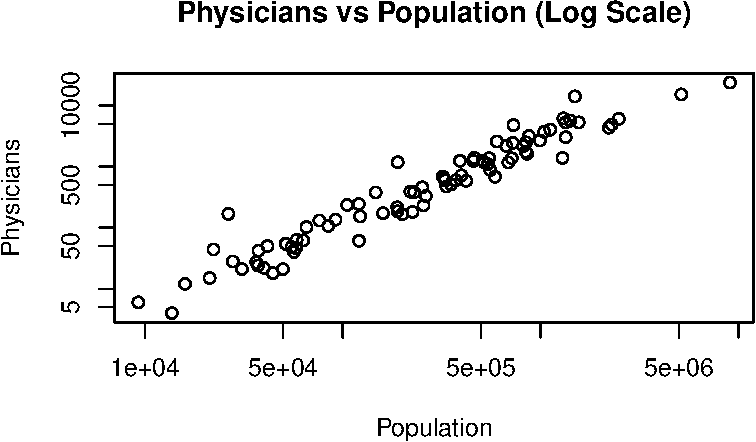
\includegraphics[keepaspectratio]{ups_files/figure-pdf/fig-statepop-phys-vs-popn-1.pdf}}

}

\caption{\label{fig-statepop-phys-vs-popn}Physicians vs.~population
(log-log scale), sample of U.S. counties}

\end{figure}%

All three estimates come from the same quantity, the ratio
\(b_j^*=\mathrm{phys}_j^*/\mathrm{popn}_j^*\) of physicians per person
of the county selected on draw \(j\). To avoid tiny numbers we measure
the population in thousands of people, so that \(b_j^*\) is the number
of physicians per 1,000 people. The function \texttt{upswr\_est} takes
the physicians and populations of the 100 draws, the population mean and
total of \(x\) (the number of counties is \(N=3141\), so
\(\bar{x}_U=t_x/N\)), and the \texttt{method}.

\emph{Physicians per 1,000 people,} \(\hat{B}_{\mathrm{HH}}=\bar{b}^*\).
The working table lists the ratios \(b_j^*\) of the first draws, their
deviations from \(\hat{B}_{\mathrm{HH}}\), and the squared deviations,
whose sum gives \(s_{b^*}^2\):

\begin{Shaded}
\begin{Highlighting}[]
\NormalTok{N }\OtherTok{\textless{}{-}} \DecValTok{3141}   \CommentTok{\# counties in the US}
\NormalTok{popn\_k }\OtherTok{\textless{}{-}}\NormalTok{ popn }\SpecialCharTok{/} \DecValTok{1000}   \CommentTok{\# population in thousands}
\NormalTok{M\_k }\OtherTok{\textless{}{-}}\NormalTok{ M }\SpecialCharTok{/} \DecValTok{1000}
\NormalTok{res\_phys\_ratio\_hh }\OtherTok{\textless{}{-}} \FunctionTok{upswr\_est}\NormalTok{(phys, popn\_k, }\AttributeTok{xbar\_pop =}\NormalTok{ M\_k }\SpecialCharTok{/}\NormalTok{ N, }\AttributeTok{tx\_pop =}\NormalTok{ M\_k, }\AttributeTok{method =} \StringTok{"ratio"}\NormalTok{)}
\NormalTok{res\_phys\_ratio\_hh}\SpecialCharTok{$}\NormalTok{table}
\end{Highlighting}
\end{Shaded}

\begin{table}[H]
\caption*{
{\large  UPSWR Hansen-Hurwitz Estimation: Working Table\normalsize } \\ 
{\normalsize  \(n = 100\)\normalsize }
} 
\normalsize
\begin{gtfit}{\linewidth}{>{\raggedright\arraybackslash}p{\dimexpr 30.00pt -2\tabcolsep-1.5\arrayrulewidth}>{\raggedleft\arraybackslash}p{\dimexpr 82.50pt -2\tabcolsep-1.5\arrayrulewidth}>{\raggedleft\arraybackslash}p{\dimexpr 82.50pt -2\tabcolsep-1.5\arrayrulewidth}>{\raggedleft\arraybackslash}p{\dimexpr 82.50pt -2\tabcolsep-1.5\arrayrulewidth}>{\raggedleft\arraybackslash}p{\dimexpr 82.50pt -2\tabcolsep-1.5\arrayrulewidth}}
\toprule
\(i\) & \(b_j^*\) & \(\hat B_{\mathrm{HH}}\) & \(b_j^*-\hat B_{\mathrm{HH}}\) & \((b_j^*-\hat B_{\mathrm{HH}})^2\)\textsuperscript{\textit{1}} \\ 
\midrule\addlinespace[2.5pt]
1 & 0.29 & 2.24 & -1.94 & 3.78 \\ 
2 & 1.96 & 2.24 & -0.28 & 0.08 \\ 
3 & 1.96 & 2.24 & -0.28 & 0.08 \\ 
4 & 0.51 & 2.24 & -1.73 & 3.00 \\ 
5 & 1.72 & 2.24 & -0.51 & 0.26 \\ 
6 & 0.87 & 2.24 & -1.36 & 1.86 \\ 
... & ... & ... & ... & ... \\ 
{\bfseries Sum} & {\bfseries 223.58} & {\bfseries 2.24} & {\bfseries 0.00} & {\bfseries 260.81} \\ 
\bottomrule
\end{gtfit}
\begin{minipage}{\linewidth}
\vspace{.05em}
\textsuperscript{\textit{1}}\(s_{b^*}^2 = \sum_i (b_j^*-\hat B_{\mathrm{HH}})^2/(n-1) = 2.63\).\\
\(\hat B_{\mathrm{HH}} = \dfrac{\sum_i b_j^*}{n} = \dfrac{223.58}{100} = 2.24\)\\
\(\mathrm{SE}(\hat B_{\mathrm{HH}}) = \dfrac{s_{b^*}}{\sqrt n} = \dfrac{1.62}{\sqrt{100}} = 0.16\)\\
\end{minipage}
\end{table}

\begin{Shaded}
\begin{Highlighting}[]
\NormalTok{res\_phys\_ratio\_hh}\SpecialCharTok{$}\NormalTok{estimate }\SpecialCharTok{|\textgreater{}} \FunctionTok{format\_est\_gt}\NormalTok{(}\StringTok{"hh\_B"}\NormalTok{)}
\end{Highlighting}
\end{Shaded}

\begin{table}[H]
\normalsize
\begin{gtfit}{0.7\linewidth}{rrrr}
\toprule
\(\hat{B}_{\mathrm{HH}}\) & \(\mathrm{SE}(\hat{B}_{\mathrm{HH}})\) & 95\% CI Lower & 95\% CI Upper \\ 
\midrule\addlinespace[2.5pt]
2.24 & 0.16 & 1.91 & 2.56 \\ 
\bottomrule
\end{gtfit}
\end{table}

\textbf{Output Note:} Each draw gives an unbiased estimate of the
national number of physicians per 1,000 people, and their average is
\(\hat{B}_{\mathrm{HH}}=2.236\) physicians per 1,000 people, with a 95\%
interval of {[}1.914, 2.558{]}.

\emph{Physicians per county,}
\(\hat{\bar{y}}_{\mathrm{HH}}=\bar{x}_U\hat{B}_{\mathrm{HH}}\), with
\(\bar{x}_U=M/N\) the average population of a county:

\begin{Shaded}
\begin{Highlighting}[]
\NormalTok{res\_phys\_county }\OtherTok{\textless{}{-}} \FunctionTok{upswr\_est}\NormalTok{(phys, popn\_k, }\AttributeTok{xbar\_pop =}\NormalTok{ M\_k }\SpecialCharTok{/}\NormalTok{ N, }\AttributeTok{tx\_pop =}\NormalTok{ M\_k,}
                             \AttributeTok{method =} \StringTok{"mean"}\NormalTok{, }\AttributeTok{show.details =} \ConstantTok{FALSE}\NormalTok{)}
\NormalTok{res\_phys\_county}\SpecialCharTok{$}\NormalTok{estimate }\SpecialCharTok{|\textgreater{}} \FunctionTok{format\_est\_gt}\NormalTok{(}\StringTok{"hh\_ybar"}\NormalTok{)}
\end{Highlighting}
\end{Shaded}

\begin{table}[H]
\normalsize
\begin{gtfit}{0.7\linewidth}{rrrr}
\toprule
\(\hat{\bar{y}}_{\mathrm{HH}}\) & \(\mathrm{SE}(\hat{\bar{y}}_{\mathrm{HH}})\) & 95\% CI Lower & 95\% CI Upper \\ 
\midrule\addlinespace[2.5pt]
181.57 & 13.18 & 155.41 & 207.72 \\ 
\bottomrule
\end{gtfit}
\end{table}

\textbf{Output Note:} This is the estimate per 1,000 people times the
average county population in thousands, \(\bar{x}_U=81.2\), and its
standard error is multiplied by the same factor. It averages over
\emph{counties}, each weighted equally, so the many small rural counties
pull it down to about 182 physicians per county.

\emph{Total physicians in the US,}
\(\hat{t}_{\mathrm{HH}}=t_x\hat{B}_{\mathrm{HH}}\), with \(t_x=M\) the
US population (in thousands):

\begin{Shaded}
\begin{Highlighting}[]
\NormalTok{res\_phys\_total }\OtherTok{\textless{}{-}} \FunctionTok{upswr\_est}\NormalTok{(phys, popn\_k, }\AttributeTok{xbar\_pop =}\NormalTok{ M\_k }\SpecialCharTok{/}\NormalTok{ N, }\AttributeTok{tx\_pop =}\NormalTok{ M\_k,}
                            \AttributeTok{method =} \StringTok{"total"}\NormalTok{, }\AttributeTok{show.details =} \ConstantTok{FALSE}\NormalTok{)}
\NormalTok{res\_phys\_total}\SpecialCharTok{$}\NormalTok{estimate }\SpecialCharTok{|\textgreater{}} \FunctionTok{format\_est\_gt}\NormalTok{(}\StringTok{"hh\_total"}\NormalTok{)}
\end{Highlighting}
\end{Shaded}

\begin{table}[H]
\normalsize
\begin{gtfit}{0.7\linewidth}{rrrr}
\toprule
\(\hat{t}_{\mathrm{HH}}\) & \(\mathrm{SE}(\hat{t}_{\mathrm{HH}})\) & 95\% CI Lower & 95\% CI Upper \\ 
\midrule\addlinespace[2.5pt]
570,304.30 & 41,401.23 & 488,155.27 & 652,453.32 \\ 
\bottomrule
\end{gtfit}
\end{table}

\textbf{Output Note:} This is the estimate per 1,000 people times the US
population in thousands, so it estimates the national total number of
physicians: about 570,304 physicians in the US, with a 95\% interval of
{[}488,155, 652,453{]}. The three estimates carry the same information:
the standard errors are in the same proportion as the estimates.

\subsubsection*{Comparison with estimates based on an SRS
sample}\label{comparison-with-estimates-based-on-an-srs-sample}
\addcontentsline{toc}{subsubsection}{Comparison with estimates based on
an SRS sample}

Let's compare our UPSWR results against estimates based on a Simple
Random Sample of 100 counties, including the ratio estimator that uses
the county population at the estimation stage.

\begin{Shaded}
\begin{Highlighting}[]
\CommentTok{\# Read SRS sample, treating {-}99 as NA}
\NormalTok{counties }\OtherTok{\textless{}{-}} \FunctionTok{read.csv}\NormalTok{(}\StringTok{"data/counties.csv"}\NormalTok{, }\AttributeTok{na.strings =} \StringTok{"{-}99"}\NormalTok{)}
\NormalTok{totpop }\OtherTok{\textless{}{-}} \DecValTok{255077536}
\NormalTok{N }\OtherTok{\textless{}{-}} \DecValTok{3141} \CommentTok{\# Total number of counties}

\CommentTok{\# 1. Naive SRS estimate for total}
\NormalTok{res\_counties\_srs }\OtherTok{\textless{}{-}} \FunctionTok{srs\_est}\NormalTok{(counties}\SpecialCharTok{$}\NormalTok{physician, }\AttributeTok{N =}\NormalTok{ N, }\AttributeTok{estimate =} \StringTok{"total"}\NormalTok{, }\AttributeTok{show.details =} \ConstantTok{FALSE}\NormalTok{)}
\NormalTok{res\_counties\_srs}\SpecialCharTok{$}\NormalTok{estimate }\SpecialCharTok{|\textgreater{}} \FunctionTok{format\_est\_gt}\NormalTok{(}\StringTok{"total"}\NormalTok{)}
\end{Highlighting}
\end{Shaded}

\begin{table}[H]
\normalsize
\begin{gtfit}{0.7\linewidth}{rrrr}
\toprule
\(\hat{t}\) & \(\mathrm{SE}(\hat{t})\) & 95\% CI Lower & 95\% CI Upper \\ 
\midrule\addlinespace[2.5pt]
933,410.97 & 491,982.79 & -42,789.62 & 1,909,611.56 \\ 
\bottomrule
\end{gtfit}
\end{table}

\begin{Shaded}
\begin{Highlighting}[]
\CommentTok{\# 2. Ratio estimate for total using SRS data}
\NormalTok{res\_counties\_ratio }\OtherTok{\textless{}{-}} \FunctionTok{ratio\_est}\NormalTok{(counties}\SpecialCharTok{$}\NormalTok{physician, counties}\SpecialCharTok{$}\NormalTok{totpop, }\AttributeTok{xbarU =}\NormalTok{ totpop}\SpecialCharTok{/}\NormalTok{N, }\AttributeTok{N =}\NormalTok{ N, }\AttributeTok{estimate =} \StringTok{"total"}\NormalTok{)}
\NormalTok{res\_counties\_ratio}\SpecialCharTok{$}\NormalTok{table}
\end{Highlighting}
\end{Shaded}

\begin{table}[H]
\caption*{
{\large  Ratio Estimation: Working Table\normalsize } \\ 
{\normalsize  \(n = 100\)\normalsize }
} 
\normalsize
\begin{gtfit}{\linewidth}{>{\raggedright\arraybackslash}p{\dimexpr 30.00pt -2\tabcolsep-1.5\arrayrulewidth}>{\raggedleft\arraybackslash}p{\dimexpr 75.00pt -2\tabcolsep-1.5\arrayrulewidth}>{\raggedleft\arraybackslash}p{\dimexpr 75.00pt -2\tabcolsep-1.5\arrayrulewidth}>{\raggedleft\arraybackslash}p{\dimexpr 75.00pt -2\tabcolsep-1.5\arrayrulewidth}>{\raggedleft\arraybackslash}p{\dimexpr 75.00pt -2\tabcolsep-1.5\arrayrulewidth}>{\raggedleft\arraybackslash}p{\dimexpr 75.00pt -2\tabcolsep-1.5\arrayrulewidth}}
\toprule
\(i\) & \(y_i\) & \(x_i\) & \(\hat y_i\)\textsuperscript{\textit{1}} & \(e_i\) & \(e_i^2\) \\ 
\midrule\addlinespace[2.5pt]
1 & 24.00 & 36,023.00 & 90.31 & -66.31 & 4,397.47 \\ 
2 & 44.00 & 73,524.00 & 184.33 & -140.33 & 19,693.17 \\ 
3 & 7.00 & 6,408.00 & 16.07 & -9.07 & 82.18 \\ 
4 & 11.00 & 19,261.00 & 48.29 & -37.29 & 1,390.49 \\ 
5 & 3.00 & 7,649.00 & 19.18 & -16.18 & 261.69 \\ 
6 & 327.00 & 188,377.00 & 472.28 & -145.28 & 21,106.52 \\ 
... & ... & ... & ... & ... & ... \\ 
{\bfseries Sum} & {\bfseries 29,717.00} & {\bfseries 11,853,116.00} & {\bfseries 29,717.00} & {\bfseries 0.00} & {\bfseries 17,054,519.52} \\ 
\bottomrule
\end{gtfit}
\begin{minipage}{\linewidth}
\vspace{.05em}
\textsuperscript{\textit{1}}\(\hat B = \sum_i y_i / \sum_i x_i = 0.00\), \(\hat y_i = \hat B\, x_i\), \(s_e^2 = 1.72 \times 10^{5}\).\\
\(\hat t = \hat B\,\bar x_U\,N = 0.00 \times 81,209.02 \times 3,141 = 6.40 \times 10^{5}\)\\
\(\mathrm{SE}(\hat t) = \mathrm{SE}(\hat B)\,\bar x_U\,N = 3.45 \times 10^{-4} \times 81,209.02 \times 3,141 = 87,885.27\)\\
\end{minipage}
\end{table}

\begin{Shaded}
\begin{Highlighting}[]
\NormalTok{res\_counties\_ratio}\SpecialCharTok{$}\NormalTok{estimate }\SpecialCharTok{|\textgreater{}} \FunctionTok{format\_est\_gt}\NormalTok{(}\StringTok{"total"}\NormalTok{)}
\end{Highlighting}
\end{Shaded}

\begin{table}[H]
\normalsize
\begin{gtfit}{0.7\linewidth}{rrrr}
\toprule
\(\hat{t}\) & \(\mathrm{SE}(\hat{t})\) & 95\% CI Lower & 95\% CI Upper \\ 
\midrule\addlinespace[2.5pt]
639,506.03 & 87,885.27 & 465,122.60 & 813,889.46 \\ 
\bottomrule
\end{gtfit}
\end{table}

\begin{Shaded}
\begin{Highlighting}[]
\CommentTok{\# 3. Regression estimate for total using SRS data}
\NormalTok{res\_counties\_reg }\OtherTok{\textless{}{-}} \FunctionTok{reg\_est}\NormalTok{(counties}\SpecialCharTok{$}\NormalTok{physician, counties}\SpecialCharTok{$}\NormalTok{totpop, }\AttributeTok{xbarU =}\NormalTok{ totpop}\SpecialCharTok{/}\NormalTok{N, }\AttributeTok{N =}\NormalTok{ N, }\AttributeTok{estimate =} \StringTok{"total"}\NormalTok{)}
\NormalTok{res\_counties\_reg}\SpecialCharTok{$}\NormalTok{table}
\end{Highlighting}
\end{Shaded}

\begin{table}[H]
\caption*{
{\large  Regression Estimation: Working Table\normalsize } \\ 
{\normalsize  \(n = 100\)\normalsize }
} 
\normalsize
\begin{gtfit}{\linewidth}{>{\raggedright\arraybackslash}p{\dimexpr 30.00pt -2\tabcolsep-1.5\arrayrulewidth}>{\raggedleft\arraybackslash}p{\dimexpr 75.00pt -2\tabcolsep-1.5\arrayrulewidth}>{\raggedleft\arraybackslash}p{\dimexpr 75.00pt -2\tabcolsep-1.5\arrayrulewidth}>{\raggedleft\arraybackslash}p{\dimexpr 75.00pt -2\tabcolsep-1.5\arrayrulewidth}>{\raggedleft\arraybackslash}p{\dimexpr 75.00pt -2\tabcolsep-1.5\arrayrulewidth}>{\raggedleft\arraybackslash}p{\dimexpr 75.00pt -2\tabcolsep-1.5\arrayrulewidth}}
\toprule
\(i\) & \(y_i\) & \(x_i\) & \(\hat y_i\)\textsuperscript{\textit{1}} & \(e_i\) & \(e_i^2\) \\ 
\midrule\addlinespace[2.5pt]
1 & 24.00 & 36,023.00 & 52.56 & -28.56 & 815.88 \\ 
2 & 44.00 & 73,524.00 & 163.74 & -119.74 & 14,337.75 \\ 
3 & 7.00 & 6,408.00 & -35.23 & 42.23 & 1,783.70 \\ 
4 & 11.00 & 19,261.00 & 2.87 & 8.13 & 66.09 \\ 
5 & 3.00 & 7,649.00 & -31.55 & 34.55 & 1,194.03 \\ 
6 & 327.00 & 188,377.00 & 504.24 & -177.24 & 31,413.03 \\ 
... & ... & ... & ... & ... & ... \\ 
{\bfseries Sum} & {\bfseries 29,717.00} & {\bfseries 11,853,116.00} & {\bfseries 29,717.00} & {\bfseries 0.00} & {\bfseries 11,349,761.43} \\ 
\bottomrule
\end{gtfit}
\begin{minipage}{\linewidth}
\vspace{.05em}
\textsuperscript{\textit{1}}\(\hat B_0 = -54.23\), \(\hat B_1 = 0.00\), \(\hat y_i = \hat B_0 + \hat B_1 x_i\), \(s_e^2 = 1.16 \times 10^{5}\).\\
\(\hat t_{reg} = N\bar y_{reg} = 3,141 \times 186.52 = 5.86 \times 10^{5}\)\\
\(\mathrm{SE}(\hat t_{reg}) = N\times\mathrm{SE}(\bar y_{reg}) = 3,141 \times 33.49 = 1.05 \times 10^{5}\)\\
\end{minipage}
\end{table}

\begin{Shaded}
\begin{Highlighting}[]
\NormalTok{res\_counties\_reg}\SpecialCharTok{$}\NormalTok{estimate }\SpecialCharTok{|\textgreater{}} \FunctionTok{format\_est\_gt}\NormalTok{(}\StringTok{"reg\_total"}\NormalTok{)}
\end{Highlighting}
\end{Shaded}

\begin{table}[H]
\normalsize
\begin{gtfit}{0.7\linewidth}{rrrr}
\toprule
\(\hat{t}_{reg}\) & \(\mathrm{SE}(\hat{t}_{reg})\) & 95\% CI Lower & 95\% CI Upper \\ 
\midrule\addlinespace[2.5pt]
585,870.60 & 105,177.42 & 377,149.44 & 794,591.76 \\ 
\bottomrule
\end{gtfit}
\end{table}

\textbf{Output Note:} The true value is \textbf{532,638}. Notice how
poorly the naive SRS estimate performs (predicting over 800,000) because
it ignores county sizes. Both the SRS Ratio and SRS Regression methods
perform much better by incorporating auxiliary population data, as does
the HH estimator above, which uses the county sizes at the design stage.

\textbf{Summary.} The estimates of the total number of physicians in the
US from all the methods above:

{

\begin{longtable}[]{@{}
  >{\raggedright\arraybackslash}p{(\linewidth - 10\tabcolsep) * \real{0.4602}}
  >{\raggedleft\arraybackslash}p{(\linewidth - 10\tabcolsep) * \real{0.0796}}
  >{\raggedleft\arraybackslash}p{(\linewidth - 10\tabcolsep) * \real{0.0708}}
  >{\raggedleft\arraybackslash}p{(\linewidth - 10\tabcolsep) * \real{0.1150}}
  >{\raggedleft\arraybackslash}p{(\linewidth - 10\tabcolsep) * \real{0.1150}}
  >{\raggedleft\arraybackslash}p{(\linewidth - 10\tabcolsep) * \real{0.1593}}@{}}

\caption{\label{tbl-statepop-summary}Estimates of the total number of
physicians in the US (true value 532,638)}

\tabularnewline

\toprule\noalign{}
\begin{minipage}[b]{\linewidth}\raggedright
Method
\end{minipage} & \begin{minipage}[b]{\linewidth}\raggedleft
Estimate
\end{minipage} & \begin{minipage}[b]{\linewidth}\raggedleft
SE
\end{minipage} & \begin{minipage}[b]{\linewidth}\raggedleft
95\% CI lower
\end{minipage} & \begin{minipage}[b]{\linewidth}\raggedleft
95\% CI upper
\end{minipage} & \begin{minipage}[b]{\linewidth}\raggedleft
Estimate \(-\) true
\end{minipage} \\
\midrule\noalign{}
\endhead
\bottomrule\noalign{}
\endlastfoot
Sample total, \(N\bar{y}\) (SRS) & 933,411 & 491,983 & -42,790 &
1,909,612 & 400,773 \\
Ratio estimator (SRS) & 639,506 & 87,885 & 465,123 & 813,889 &
106,868 \\
Regression estimator (SRS) & 585,871 & 105,177 & 377,149 & 794,592 &
53,233 \\
Hansen--Hurwitz, \(t_x\hat{B}_{\mathrm{HH}}\) (UPSWR) & 570,304 & 41,401
& 488,155 & 652,453 & 37,666 \\

\end{longtable}

}

The naive SRS total ignores the county sizes: it is far too large, with
a huge SE. The ratio and regression estimators use the county
populations at the estimation stage and have much smaller SEs, and HH,
which uses them at the design stage, has the smallest SE and the
smallest error here, even though its sample is of the same size, 100
counties.

\subsection{\texorpdfstring{Simulation Study using \texttt{agpop}
Data}{Simulation Study using agpop Data}}\label{sec-ups-sim}

Let's simulate 2000 random samples of 300 counties to see how UPSWR,
with \(\psi_i\) proportional to the acres in 1987 (\(x_i\)), empirically
compares to SRS for estimating the total acres in 1992 (\(y_i\)).

\begin{Shaded}
\begin{Highlighting}[]
\CommentTok{\# Read population data}
\NormalTok{agpop }\OtherTok{\textless{}{-}} \FunctionTok{acres\_in\_thousands}\NormalTok{(}\FunctionTok{read.csv}\NormalTok{(}\StringTok{"data/agpop.csv"}\NormalTok{, }\AttributeTok{na.strings =} \StringTok{"{-}99"}\NormalTok{))}
\NormalTok{agpop }\OtherTok{\textless{}{-}}\NormalTok{ agpop }\SpecialCharTok{|\textgreater{}} \FunctionTok{filter}\NormalTok{(}\SpecialCharTok{!}\FunctionTok{is.na}\NormalTok{(acres92), }\SpecialCharTok{!}\FunctionTok{is.na}\NormalTok{(acres87))}

\NormalTok{N }\OtherTok{\textless{}{-}} \FunctionTok{nrow}\NormalTok{(agpop)}
\NormalTok{total\_acres92 }\OtherTok{\textless{}{-}} \FunctionTok{sum}\NormalTok{(agpop}\SpecialCharTok{$}\NormalTok{acres92)}
\NormalTok{total\_acres87 }\OtherTok{\textless{}{-}} \FunctionTok{sum}\NormalTok{(agpop}\SpecialCharTok{$}\NormalTok{acres87)}
\NormalTok{acres87 }\OtherTok{\textless{}{-}}\NormalTok{ agpop}\SpecialCharTok{$}\NormalTok{acres87}

\CommentTok{\# Storage vectors for simulation}
\NormalTok{est\_srs300 }\OtherTok{\textless{}{-}} \FunctionTok{rep}\NormalTok{(}\DecValTok{0}\NormalTok{, }\DecValTok{2000}\NormalTok{)}
\NormalTok{est\_srs300\_reg\_acres87 }\OtherTok{\textless{}{-}} \FunctionTok{rep}\NormalTok{(}\DecValTok{0}\NormalTok{, }\DecValTok{2000}\NormalTok{)}
\NormalTok{est\_srs300\_ratio\_acres87 }\OtherTok{\textless{}{-}} \FunctionTok{rep}\NormalTok{(}\DecValTok{0}\NormalTok{, }\DecValTok{2000}\NormalTok{)}
\NormalTok{est\_ups300\_acres87 }\OtherTok{\textless{}{-}} \FunctionTok{rep}\NormalTok{(}\DecValTok{0}\NormalTok{, }\DecValTok{2000}\NormalTok{)}

\ControlFlowTok{for}\NormalTok{ (i }\ControlFlowTok{in} \DecValTok{1}\SpecialCharTok{:}\DecValTok{2000}\NormalTok{) \{}
  \CommentTok{\# SRS Simulation}
\NormalTok{  srs300 }\OtherTok{\textless{}{-}} \FunctionTok{sample}\NormalTok{(}\DecValTok{1}\SpecialCharTok{:}\NormalTok{N, }\AttributeTok{size =} \DecValTok{300}\NormalTok{)}
\NormalTok{  acres92\_srs300 }\OtherTok{\textless{}{-}}\NormalTok{ agpop}\SpecialCharTok{$}\NormalTok{acres92[srs300]}
\NormalTok{  acres87\_srs300 }\OtherTok{\textless{}{-}}\NormalTok{ agpop}\SpecialCharTok{$}\NormalTok{acres87[srs300]}

\NormalTok{  est\_srs300[i] }\OtherTok{\textless{}{-}} \FunctionTok{srs\_est}\NormalTok{(acres92\_srs300, }\AttributeTok{N =}\NormalTok{ N, }\AttributeTok{estimate =} \StringTok{"total"}\NormalTok{, }\AttributeTok{show.details =} \ConstantTok{FALSE}\NormalTok{)}\SpecialCharTok{$}\NormalTok{estimate[}\DecValTok{1}\NormalTok{]}
\NormalTok{  est\_srs300\_reg\_acres87[i] }\OtherTok{\textless{}{-}} \FunctionTok{reg\_est}\NormalTok{(acres92\_srs300, acres87\_srs300,}
                                           \AttributeTok{xbarU =}\NormalTok{ total\_acres87}\SpecialCharTok{/}\NormalTok{N, }\AttributeTok{N =}\NormalTok{ N, }\AttributeTok{estimate =} \StringTok{"total"}\NormalTok{, }\AttributeTok{show.details =} \ConstantTok{FALSE}\NormalTok{)}\SpecialCharTok{$}\NormalTok{estimate[}\DecValTok{1}\NormalTok{]}

\NormalTok{  est\_srs300\_ratio\_acres87[i] }\OtherTok{\textless{}{-}} \FunctionTok{ratio\_est}\NormalTok{(acres92\_srs300, acres87\_srs300,}
                                           \AttributeTok{xbarU =}\NormalTok{ total\_acres87}\SpecialCharTok{/}\NormalTok{N, }\AttributeTok{N =}\NormalTok{ N, }\AttributeTok{estimate =} \StringTok{"total"}\NormalTok{, }\AttributeTok{show.details =} \ConstantTok{FALSE}\NormalTok{)}\SpecialCharTok{$}\NormalTok{estimate[}\DecValTok{1}\NormalTok{]}

  \CommentTok{\# UPSWR Simulation (Probability proportional to acres87)}
\NormalTok{  ups300 }\OtherTok{\textless{}{-}} \FunctionTok{sample}\NormalTok{(}\DecValTok{1}\SpecialCharTok{:}\NormalTok{N, }\AttributeTok{size =} \DecValTok{300}\NormalTok{, }\AttributeTok{prob =}\NormalTok{ acres87, }\AttributeTok{replace =} \ConstantTok{TRUE}\NormalTok{)}
\NormalTok{  acres92\_ups300 }\OtherTok{\textless{}{-}}\NormalTok{ agpop}\SpecialCharTok{$}\NormalTok{acres92[ups300]}

\NormalTok{  psi }\OtherTok{\textless{}{-}}\NormalTok{ (acres87 }\SpecialCharTok{/} \FunctionTok{sum}\NormalTok{(acres87))[ups300]}
\NormalTok{  est\_ups300\_acres87[i] }\OtherTok{\textless{}{-}} \FunctionTok{upswr\_total}\NormalTok{(acres92\_ups300, psi, }\AttributeTok{show.details =} \ConstantTok{FALSE}\NormalTok{)}\SpecialCharTok{$}\NormalTok{estimate[}\DecValTok{1}\NormalTok{]}
\NormalTok{\}}
\end{Highlighting}
\end{Shaded}

\begin{figure}

\centering{

\pandocbounded{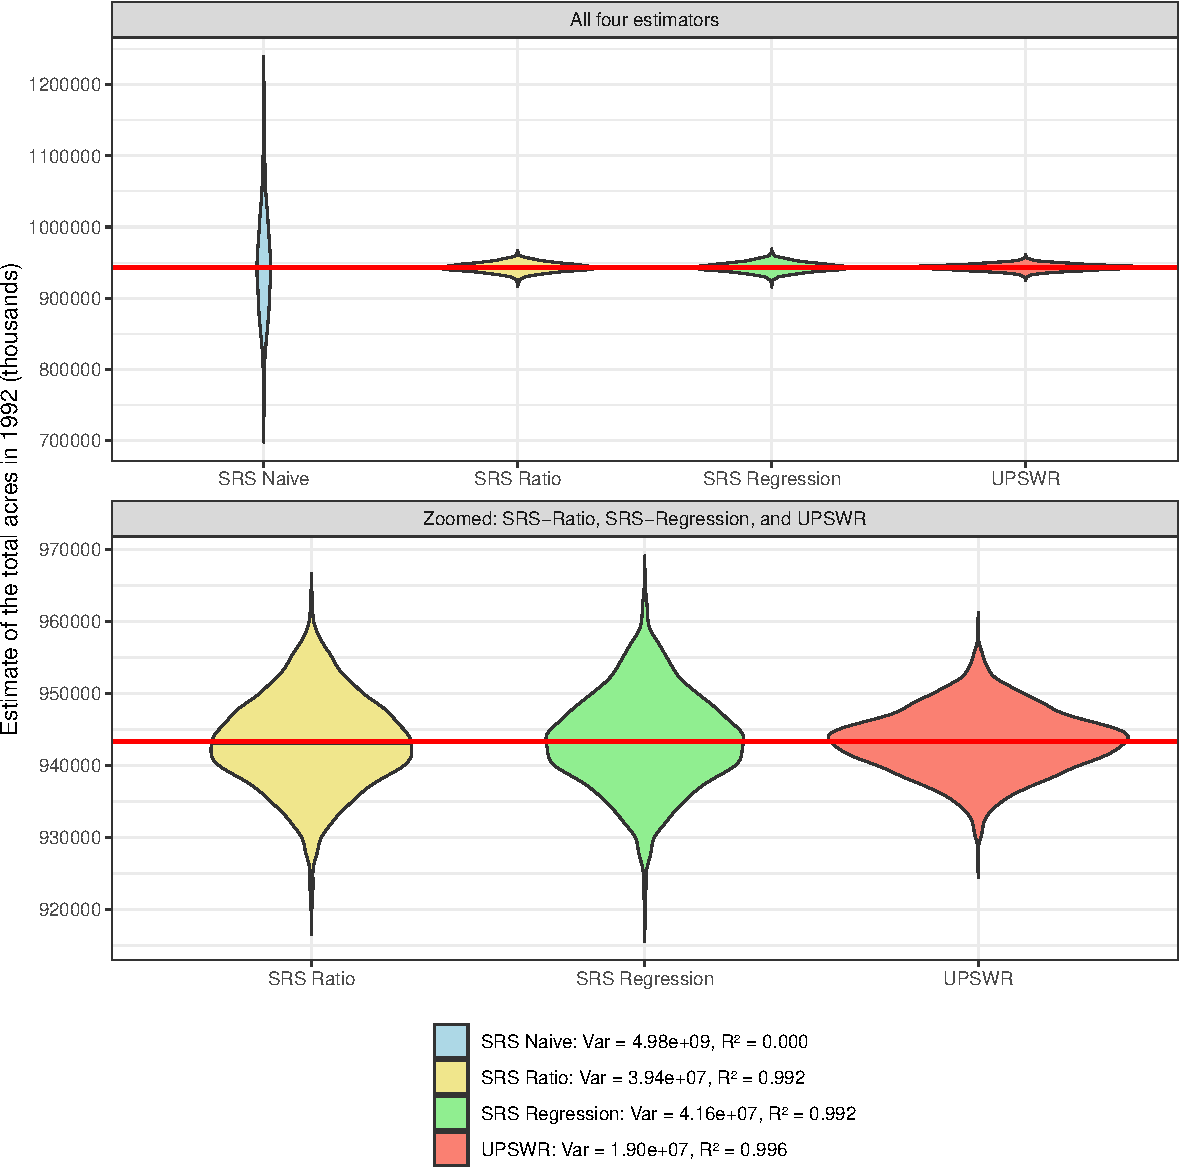
\includegraphics[keepaspectratio]{ups_files/figure-pdf/fig-upswr-sim-comparison-1.pdf}}

}

\caption{\label{fig-upswr-sim-comparison}Estimator distribution: naive
SRS vs.~SRS ratio vs.~SRS regression vs.~UPSWR (2000 simulations), full
and zoomed views. The legend gives the variance of each estimator and
its \(R^2\) relative to the naive SRS average.}

\end{figure}%

\textbf{Output Note:} The red line represents the true total acreage,
and the line inside each violin is the median. The naive SRS estimator
has massive variance. The SRS ratio and regression estimators, which use
the 1987 acres at the estimation stage, and UPSWR, which uses them at
the design stage, drastically reduce the variance, centering tightly
around the true mean; the \(R^2\) in the legend is the proportion of the
variance of the naive SRS average that each method removes.

\subsection{Shinylive App Comparing SRS and UPSWR}\label{sec-ups-app}

The same simulation runs as a standalone app:
\href{../shinylives_sampling/app-ups.html}{SRS (average and ratio) with
UPSWR (Hansen--Hurwitz) and UPSWO (Horvitz--Thompson)}. It opens in a
new tab, together with its documentation and the full
\href{../shinylives_sampling/index.html}{list of apps}. Its ``Variance
reduction vs.~SRS average'' legend reports the variances of the ratio,
HH and HT estimators, simulated and theoretical, relative to the plain
SRS average, and illustrates the comparison of the variances in
Section~\ref{sec-ups-compare}. The app describes all the estimators
through the ratios \(b_i\), and for the UPSWO estimator it shows the
coverage of the confidence intervals based on the Hájek and the
with-replacement variance estimators (Section~\ref{sec-ups-wo}).

\section{One-Stage Cluster Sampling with PPS}\label{sec-ups-cluster}

\subsection{Theory}\label{sec-ups-cluster-theory}

In cluster sampling, the units of the HH estimator are \textbf{clusters}
(primary sampling units, psus), and the study value of unit \(i\) is the
\textbf{cluster total} \(t_i=\sum_{j=1}^{M_i}y_{ij}\). In a one-stage
design, every element (secondary sampling unit, ssu) of a selected
cluster is observed, so \(t_i\) is known for the sampled clusters. The
auxiliary variable is the \textbf{cluster size} \(M_i\), known for all
clusters. So the notation of Section~\ref{sec-ups-hh-theory} changes as
\[
y_i \to t_i,\qquad x_i\to M_i,\qquad t_x\to M_0=\sum_{i=1}^N M_i,\qquad \bar{x}_U\to\bar{M}_U=\frac{M_0}{N},
\qquad \psi_i=\frac{M_i}{M_0}.
\] The ratio of cluster \(i\) is \[
b_i=\frac{t_i}{M_i}=\bar{y}_i ,
\] the \textbf{mean per element (ssu-level mean)} of cluster \(i\), and
\(B=t/M_0\) is the mean per element of the whole population, which we
denote also by \(\bar{y}_U\). Let \(b_j^*=\bar{y}_j^*\) be the mean per
element of the cluster selected on draw \(j\). Then everything in
Section~\ref{sec-ups-hh-theory} applies:

\[
\boxed{\hat{B}_{\mathrm{HH}}=\bar{b}^*=\frac{1}{n}\sum_{j=1}^n \bar{y}_j^*},\qquad
\widehat{\mathrm{SE}}(\hat{B}_{\mathrm{HH}})=\frac{s_{b^*}}{\sqrt{n}},\qquad
s_{b^*}^2=\frac{1}{n-1}\sum_{j=1}^n\left(\bar{y}_j^*-\bar{b}^*\right)^2 .
\]

That is, the estimate of the mean per element is the plain average of
the means of the sampled clusters: large clusters are selected more
often, and each selected cluster is then weighted equally. Multiplying
by the known constants gives the estimates of the three quantities of
interest, with their estimated SEs multiplied by the same constants:

{\def\LTcaptype{none} % do not increment counter
\begin{longtable}[]{@{}
  >{\raggedright\arraybackslash}p{(\linewidth - 4\tabcolsep) * \real{0.3333}}
  >{\raggedright\arraybackslash}p{(\linewidth - 4\tabcolsep) * \real{0.3333}}
  >{\raggedright\arraybackslash}p{(\linewidth - 4\tabcolsep) * \real{0.3333}}@{}}
\toprule\noalign{}
\begin{minipage}[b]{\linewidth}\raggedright
Quantity
\end{minipage} & \begin{minipage}[b]{\linewidth}\raggedright
Estimate
\end{minipage} & \begin{minipage}[b]{\linewidth}\raggedright
Estimated SE
\end{minipage} \\
\midrule\noalign{}
\endhead
\bottomrule\noalign{}
\endlastfoot
Mean per element, \(\bar{y}_U=B=t/M_0\) & \(\hat{B}_{\mathrm{HH}}\) &
\(s_{b^*}/\sqrt{n}\) \\
Mean per cluster (psu-level mean), \(\bar{t}_U=t/N\) &
\(\bar{M}_U\,\hat{B}_{\mathrm{HH}}\) &
\(\bar{M}_U\,s_{b^*}/\sqrt{n}\) \\
Total, \(t=\sum_{i=1}^N t_i\) & \(M_0\,\hat{B}_{\mathrm{HH}}\) &
\(M_0\,s_{b^*}/\sqrt{n}\) \\
\end{longtable}
}

The estimator is most precise when the cluster means \(\bar{y}_i\) vary
little, that is, when \(t_i\) is nearly proportional to \(M_i\). Note
that this differs from the ratio estimator
\(\sum_{i\in\mathcal{S}}t_i/\sum_{i\in\mathcal{S}}M_i\) of cluster
sampling with a simple random sample of clusters: here the cluster sizes
have been used at the design stage, so a plain average replaces the
ratio.

\subsection{Example: Falls in Long-Term Care
Homes}\label{sec-ups-cluster-example}

A health authority wants to estimate the number of falls over the past
year of the residents of its \(N=40\) long-term care homes. From the
registry it knows the number of residents \(M_i\) of every home, and
\(M_0=3{,}000\) residents in total, so \(\bar{M}_U=M_0/N=75\) residents
per home. Visiting a home to review the incident reports of all its
residents is costly, so \(n=8\) draws of homes are made with replacement
with probabilities \(\psi_i=M_i/M_0\) proportional to the number of
residents. The sample is a one-stage cluster sample: every resident of a
selected home is reviewed, and \(t_i\) is the number of falls in home
\(i\). (The data are made up for illustration.) Home H12 was drawn
twice; a repeated draw is kept as a separate observation, and since all
its residents are reviewed, it has the same \(t_i\):

{

\begin{longtable}[]{@{}
  >{\raggedleft\arraybackslash}p{(\linewidth - 10\tabcolsep) * \real{0.0804}}
  >{\raggedright\arraybackslash}p{(\linewidth - 10\tabcolsep) * \real{0.0446}}
  >{\raggedleft\arraybackslash}p{(\linewidth - 10\tabcolsep) * \real{0.1786}}
  >{\raggedleft\arraybackslash}p{(\linewidth - 10\tabcolsep) * \real{0.1875}}
  >{\raggedleft\arraybackslash}p{(\linewidth - 10\tabcolsep) * \real{0.1429}}
  >{\raggedleft\arraybackslash}p{(\linewidth - 10\tabcolsep) * \real{0.3661}}@{}}

\caption{\label{tbl-falls-data}Falls in the sampled long-term care
homes, \(n=8\) draws}

\tabularnewline

\toprule\noalign{}
\begin{minipage}[b]{\linewidth}\raggedleft
Draw \(j\)
\end{minipage} & \begin{minipage}[b]{\linewidth}\raggedright
Home
\end{minipage} & \begin{minipage}[b]{\linewidth}\raggedleft
\(M_j^*\) (residents)
\end{minipage} & \begin{minipage}[b]{\linewidth}\raggedleft
\(\psi_j^*=M_j^*/M_0\)
\end{minipage} & \begin{minipage}[b]{\linewidth}\raggedleft
\(t_j^*\) (falls)
\end{minipage} & \begin{minipage}[b]{\linewidth}\raggedleft
\(b_j^*=t_j^*/M_j^*\) (falls per resident)
\end{minipage} \\
\midrule\noalign{}
\endhead
\bottomrule\noalign{}
\endlastfoot
1 & H12 & 180 & 0.060 & 160 & 0.8889 \\
2 & H03 & 60 & 0.020 & 49 & 0.8167 \\
3 & H27 & 240 & 0.080 & 205 & 0.8542 \\
4 & H12 & 180 & 0.060 & 160 & 0.8889 \\
5 & H31 & 95 & 0.032 & 70 & 0.7368 \\
6 & H08 & 120 & 0.040 & 118 & 0.9833 \\
7 & H19 & 45 & 0.015 & 30 & 0.6667 \\
8 & H36 & 150 & 0.050 & 140 & 0.9333 \\

\end{longtable}

}

We estimate \(B\), the number of falls per resident, with
\texttt{upswr\_est}, using the totals \(t_i\) of the sampled homes as
\texttt{ydata} and their sizes \(M_i\) as \texttt{xdata}. The working
table lists the cluster means \(b_j^*\), their deviations from
\(\hat{B}_{\mathrm{HH}}\), and the squared deviations:

\begin{Shaded}
\begin{Highlighting}[]
\NormalTok{res\_falls\_B }\OtherTok{\textless{}{-}} \FunctionTok{upswr\_est}\NormalTok{(ti, Mi, }\AttributeTok{xbar\_pop =}\NormalTok{ Mbar\_U, }\AttributeTok{tx\_pop =}\NormalTok{ M0, }\AttributeTok{method =} \StringTok{"ratio"}\NormalTok{, }\AttributeTok{decimals =} \DecValTok{4}\NormalTok{)}
\NormalTok{res\_falls\_B}\SpecialCharTok{$}\NormalTok{table}
\end{Highlighting}
\end{Shaded}

\begin{table}[H]
\caption*{
{\large  UPSWR Hansen-Hurwitz Estimation: Working Table\normalsize } \\ 
{\normalsize  \(n = 8\)\normalsize }
} 
\normalsize
\begin{gtfit}{\linewidth}{>{\raggedright\arraybackslash}p{\dimexpr 30.00pt -2\tabcolsep-1.5\arrayrulewidth}>{\raggedleft\arraybackslash}p{\dimexpr 82.50pt -2\tabcolsep-1.5\arrayrulewidth}>{\raggedleft\arraybackslash}p{\dimexpr 82.50pt -2\tabcolsep-1.5\arrayrulewidth}>{\raggedleft\arraybackslash}p{\dimexpr 82.50pt -2\tabcolsep-1.5\arrayrulewidth}>{\raggedleft\arraybackslash}p{\dimexpr 82.50pt -2\tabcolsep-1.5\arrayrulewidth}}
\toprule
\(i\) & \(b_j^*\) & \(\hat B_{\mathrm{HH}}\) & \(b_j^*-\hat B_{\mathrm{HH}}\) & \((b_j^*-\hat B_{\mathrm{HH}})^2\)\textsuperscript{\textit{1}} \\ 
\midrule\addlinespace[2.5pt]
1 & 0.8889 & 0.8461 & 0.0428 & 0.0018 \\ 
2 & 0.8167 & 0.8461 & -0.0294 & 0.0009 \\ 
3 & 0.8542 & 0.8461 & 0.0081 & 0.0001 \\ 
4 & 0.8889 & 0.8461 & 0.0428 & 0.0018 \\ 
5 & 0.7368 & 0.8461 & -0.1093 & 0.0119 \\ 
6 & 0.9833 & 0.8461 & 0.1372 & 0.0188 \\ 
... & ... & ... & ... & ... \\ 
{\bfseries Sum} & {\bfseries 6.7688} & {\bfseries 0.8461} & {\bfseries 0.0000} & {\bfseries 0.0752} \\ 
\bottomrule
\end{gtfit}
\begin{minipage}{\linewidth}
\vspace{.05em}
\textsuperscript{\textit{1}}\(s_{b^*}^2 = \sum_i (b_j^*-\hat B_{\mathrm{HH}})^2/(n-1) = 0.0107\).\\
\(\hat B_{\mathrm{HH}} = \dfrac{\sum_i b_j^*}{n} = \dfrac{6.7688}{8} = 0.8461\)\\
\(\mathrm{SE}(\hat B_{\mathrm{HH}}) = \dfrac{s_{b^*}}{\sqrt n} = \dfrac{0.1036}{\sqrt{8}} = 0.0366\)\\
\end{minipage}
\end{table}

\begin{Shaded}
\begin{Highlighting}[]
\NormalTok{res\_falls\_B}\SpecialCharTok{$}\NormalTok{estimate }\SpecialCharTok{|\textgreater{}} \FunctionTok{format\_est\_gt}\NormalTok{(}\StringTok{"hh\_B"}\NormalTok{)}
\end{Highlighting}
\end{Shaded}

\begin{table}[H]
\normalsize
\begin{gtfit}{0.7\linewidth}{rrrr}
\toprule
\(\hat{B}_{\mathrm{HH}}\) & \(\mathrm{SE}(\hat{B}_{\mathrm{HH}})\) & 95\% CI Lower & 95\% CI Upper \\ 
\midrule\addlinespace[2.5pt]
0.85 & 0.04 & 0.76 & 0.93 \\ 
\bottomrule
\end{gtfit}
\end{table}

Then we multiply by \(\bar{M}_U=75\) for the number of falls per home,
and by \(M_0=3{,}000\) for the total number of falls:

\begin{Shaded}
\begin{Highlighting}[]
\NormalTok{res\_falls\_home }\OtherTok{\textless{}{-}} \FunctionTok{upswr\_est}\NormalTok{(ti, Mi, }\AttributeTok{xbar\_pop =}\NormalTok{ Mbar\_U, }\AttributeTok{tx\_pop =}\NormalTok{ M0, }\AttributeTok{method =} \StringTok{"mean"}\NormalTok{, }\AttributeTok{show.details =} \ConstantTok{FALSE}\NormalTok{)}
\NormalTok{res\_falls\_home}\SpecialCharTok{$}\NormalTok{estimate }\SpecialCharTok{|\textgreater{}} \FunctionTok{format\_est\_gt}\NormalTok{(}\StringTok{"hh\_ybar"}\NormalTok{)}
\end{Highlighting}
\end{Shaded}

\begin{table}[H]
\normalsize
\begin{gtfit}{0.7\linewidth}{rrrr}
\toprule
\(\hat{\bar{y}}_{\mathrm{HH}}\) & \(\mathrm{SE}(\hat{\bar{y}}_{\mathrm{HH}})\) & 95\% CI Lower & 95\% CI Upper \\ 
\midrule\addlinespace[2.5pt]
63.46 & 2.75 & 56.96 & 69.95 \\ 
\bottomrule
\end{gtfit}
\end{table}

\begin{Shaded}
\begin{Highlighting}[]
\NormalTok{res\_falls\_total }\OtherTok{\textless{}{-}} \FunctionTok{upswr\_est}\NormalTok{(ti, Mi, }\AttributeTok{xbar\_pop =}\NormalTok{ Mbar\_U, }\AttributeTok{tx\_pop =}\NormalTok{ M0, }\AttributeTok{method =} \StringTok{"total"}\NormalTok{, }\AttributeTok{show.details =} \ConstantTok{FALSE}\NormalTok{)}
\NormalTok{res\_falls\_total}\SpecialCharTok{$}\NormalTok{estimate }\SpecialCharTok{|\textgreater{}} \FunctionTok{format\_est\_gt}\NormalTok{(}\StringTok{"hh\_total"}\NormalTok{)}
\end{Highlighting}
\end{Shaded}

\begin{table}[H]
\normalsize
\begin{gtfit}{0.7\linewidth}{rrrr}
\toprule
\(\hat{t}_{\mathrm{HH}}\) & \(\mathrm{SE}(\hat{t}_{\mathrm{HH}})\) & 95\% CI Lower & 95\% CI Upper \\ 
\midrule\addlinespace[2.5pt]
2,538.29 & 109.91 & 2,278.39 & 2,798.20 \\ 
\bottomrule
\end{gtfit}
\end{table}

\textbf{Output Note:} The estimated number of falls per resident is
\(\hat{B}_{\mathrm{HH}}=0.846\) (SE 0.037), the plain average of the
eight cluster means in the working table. A typical home has
\(\bar{M}_U\hat{B}_{\mathrm{HH}}=63.5\) falls per year (SE 2.7), and the
40 homes together have about \(M_0\hat{B}_{\mathrm{HH}}=2,538\) falls
(SE 110, 95\% interval {[}2,278, 2,798{]}). The three statements carry
the same information: the estimates and the standard errors are in the
same proportion.

\section{Two-Stage Cluster Sampling with PPS}\label{sec-ups-twostage}

\subsection{Theory}\label{sec-ups-twostage-theory}

In a two-stage design, we select \(n\) clusters with replacement with
probabilities \(\psi_i=M_i/M_0\), and then take a simple random sample
of \(m_i\) elements from the \(M_i\) elements of the cluster \textbf{on
every draw}. The cluster total \(t_i\) is no longer observed, so we
cannot compute the cluster mean \(b_i=t_i/M_i\) of
Section~\ref{sec-ups-cluster-theory}. We estimate it from the subsample,
\[
\bar{y}_i=\frac{1}{m_i}\sum_{j=1}^{m_i}y_{ij},\qquad \hat{t}_i=M_i\,\bar{y}_i ,
\] where \(\bar{y}_i\) is the mean of the \emph{subsample}. The
one-stage formulas carry over with the subsample mean \(\bar{y}_j^*\) of
draw \(j\) in place of the cluster mean \(b_j^*\): \[
\boxed{\hat{B}_{\mathrm{HH}}=\bar{y}^*=\frac{1}{n}\sum_{j=1}^n \bar{y}_j^*},\qquad
\widehat{\mathrm{SE}}(\hat{B}_{\mathrm{HH}})=\frac{s_{\bar{y}^*}}{\sqrt{n}},\qquad
s_{\bar{y}^*}^2=\frac{1}{n-1}\sum_{j=1}^n\left(\bar{y}_j^*-\bar{y}^*\right)^2 ,
\] and the estimates of the mean per element, the mean per cluster and
the total are \(\hat{B}_{\mathrm{HH}}\),
\(\bar{M}_U\hat{B}_{\mathrm{HH}}\) and \(M_0\hat{B}_{\mathrm{HH}}\),
with their SEs multiplied by the same constants, as in the table of
Section~\ref{sec-ups-cluster-theory}. Equivalently, each draw estimates
the total by \(\hat{t}_j^*/\psi_j^*=M_0\,\bar{y}_j^*\).

There are two differences from the one-stage case. First, a cluster that
is drawn twice is subsampled \textbf{independently} on each draw, so the
two draws give different subsample means \(\bar{y}_j^*\), and both are
kept as separate observations. Second, \textbf{no second-stage formula
is needed for the standard error.} The \(n\) draws are independent, and
the values \(\bar{y}_j^*\) differ between draws for two reasons, the
choice of the clusters and the choice of the elements within them. The
sample variance \(s_{\bar{y}^*}^2\) of the values \(\bar{y}_j^*\)
captures both, so the variance of the two-stage estimator is computed in
exactly the same way as that of the one-stage estimator. This is a major
simplification compared with two-stage SRS of clusters, where the
variance has a between-cluster and a within-cluster piece. Of course, a
larger subsample \(m_i\) makes \(\bar{y}_i\) closer to \(t_i/M_i\) and
reduces the variance, but it does so through \(s_{\bar{y}^*}^2\).

\subsection{Example: Falls in Long-Term Care Homes, Two
Stages}\label{sec-ups-twostage-example}

Suppose the health authority of Section~\ref{sec-ups-cluster-example}
cannot afford to review all the residents of a selected home. On each of
the same \(n=8\) draws of homes, with probabilities \(\psi_i=M_i/M_0\),
a simple random sample of \(m_i\) residents is drawn, and the number of
falls of each sampled resident over the past year is recorded. The data
below are made up for illustration. Home H12 was drawn twice, and the
two subsamples were drawn independently, so the two draws have different
subsample means. The table gives the total number of falls of the
\(m_j^*\) sampled residents, their mean \(\bar{y}_j^*\), and the
estimated total of the home \(\hat{t}_j^*=M_j^*\bar{y}_j^*\):

{

\begin{longtable}[]{@{}
  >{\raggedleft\arraybackslash}p{(\linewidth - 14\tabcolsep) * \real{0.0783}}
  >{\raggedright\arraybackslash}p{(\linewidth - 14\tabcolsep) * \real{0.0435}}
  >{\raggedleft\arraybackslash}p{(\linewidth - 14\tabcolsep) * \real{0.0696}}
  >{\raggedleft\arraybackslash}p{(\linewidth - 14\tabcolsep) * \real{0.1826}}
  >{\raggedleft\arraybackslash}p{(\linewidth - 14\tabcolsep) * \real{0.0696}}
  >{\raggedleft\arraybackslash}p{(\linewidth - 14\tabcolsep) * \real{0.1652}}
  >{\raggedleft\arraybackslash}p{(\linewidth - 14\tabcolsep) * \real{0.1217}}
  >{\raggedleft\arraybackslash}p{(\linewidth - 14\tabcolsep) * \real{0.2696}}@{}}

\caption{\label{tbl-falls2-data}Two-stage sample of long-term care
homes, \(n=8\) draws}

\tabularnewline

\toprule\noalign{}
\begin{minipage}[b]{\linewidth}\raggedleft
Draw \(j\)
\end{minipage} & \begin{minipage}[b]{\linewidth}\raggedright
Home
\end{minipage} & \begin{minipage}[b]{\linewidth}\raggedleft
\(M_j^*\)
\end{minipage} & \begin{minipage}[b]{\linewidth}\raggedleft
\(\psi_j^*=M_j^*/M_0\)
\end{minipage} & \begin{minipage}[b]{\linewidth}\raggedleft
\(m_j^*\)
\end{minipage} & \begin{minipage}[b]{\linewidth}\raggedleft
Falls in subsample
\end{minipage} & \begin{minipage}[b]{\linewidth}\raggedleft
\(\bar{y}_j^*\)
\end{minipage} & \begin{minipage}[b]{\linewidth}\raggedleft
\(\hat{t}_j^*=M_j^*\bar{y}_j^*\)
\end{minipage} \\
\midrule\noalign{}
\endhead
\bottomrule\noalign{}
\endlastfoot
1 & H12 & 180 & 0.060 & 20 & 19 & 0.950 & 171.0 \\
2 & H03 & 60 & 0.020 & 20 & 15 & 0.750 & 45.0 \\
3 & H27 & 240 & 0.080 & 20 & 16 & 0.800 & 192.0 \\
4 & H12 & 180 & 0.060 & 20 & 16 & 0.800 & 144.0 \\
5 & H31 & 95 & 0.032 & 20 & 18 & 0.900 & 85.5 \\
6 & H08 & 120 & 0.040 & 20 & 21 & 1.050 & 126.0 \\
7 & H19 & 45 & 0.015 & 15 & 10 & 0.667 & 30.0 \\
8 & H36 & 150 & 0.050 & 20 & 17 & 0.850 & 127.5 \\

\end{longtable}

}

The data enter \texttt{upswr\_est} through the estimated totals
\(\hat{t}_j^*\) (as \texttt{ydata}) and the sizes \(M_j^*\) (as
\texttt{xdata}), whose ratios are the subsample means \(\bar{y}_j^*\).
The working table lists them, their deviations from
\(\hat{B}_{\mathrm{HH}}\) and the squared deviations:

\begin{Shaded}
\begin{Highlighting}[]
\NormalTok{res\_falls2\_B }\OtherTok{\textless{}{-}} \FunctionTok{upswr\_est}\NormalTok{(ti\_hat2, Mi2, }\AttributeTok{xbar\_pop =}\NormalTok{ Mbar\_U, }\AttributeTok{tx\_pop =}\NormalTok{ M0, }\AttributeTok{method =} \StringTok{"ratio"}\NormalTok{, }\AttributeTok{decimals =} \DecValTok{4}\NormalTok{)}
\NormalTok{res\_falls2\_B}\SpecialCharTok{$}\NormalTok{table}
\end{Highlighting}
\end{Shaded}

\begin{table}[H]
\caption*{
{\large  UPSWR Hansen-Hurwitz Estimation: Working Table\normalsize } \\ 
{\normalsize  \(n = 8\)\normalsize }
} 
\normalsize
\begin{gtfit}{\linewidth}{>{\raggedright\arraybackslash}p{\dimexpr 30.00pt -2\tabcolsep-1.5\arrayrulewidth}>{\raggedleft\arraybackslash}p{\dimexpr 82.50pt -2\tabcolsep-1.5\arrayrulewidth}>{\raggedleft\arraybackslash}p{\dimexpr 82.50pt -2\tabcolsep-1.5\arrayrulewidth}>{\raggedleft\arraybackslash}p{\dimexpr 82.50pt -2\tabcolsep-1.5\arrayrulewidth}>{\raggedleft\arraybackslash}p{\dimexpr 82.50pt -2\tabcolsep-1.5\arrayrulewidth}}
\toprule
\(i\) & \(b_j^*\) & \(\hat B_{\mathrm{HH}}\) & \(b_j^*-\hat B_{\mathrm{HH}}\) & \((b_j^*-\hat B_{\mathrm{HH}})^2\)\textsuperscript{\textit{1}} \\ 
\midrule\addlinespace[2.5pt]
1 & 0.9500 & 0.8458 & 0.1042 & 0.0109 \\ 
2 & 0.7500 & 0.8458 & -0.0958 & 0.0092 \\ 
3 & 0.8000 & 0.8458 & -0.0458 & 0.0021 \\ 
4 & 0.8000 & 0.8458 & -0.0458 & 0.0021 \\ 
5 & 0.9000 & 0.8458 & 0.0542 & 0.0029 \\ 
6 & 1.0500 & 0.8458 & 0.2042 & 0.0417 \\ 
... & ... & ... & ... & ... \\ 
{\bfseries Sum} & {\bfseries 6.7667} & {\bfseries 0.8458} & {\bfseries 0.0000} & {\bfseries 0.1010} \\ 
\bottomrule
\end{gtfit}
\begin{minipage}{\linewidth}
\vspace{.05em}
\textsuperscript{\textit{1}}\(s_{b^*}^2 = \sum_i (b_j^*-\hat B_{\mathrm{HH}})^2/(n-1) = 0.0144\).\\
\(\hat B_{\mathrm{HH}} = \dfrac{\sum_i b_j^*}{n} = \dfrac{6.7667}{8} = 0.8458\)\\
\(\mathrm{SE}(\hat B_{\mathrm{HH}}) = \dfrac{s_{b^*}}{\sqrt n} = \dfrac{0.1201}{\sqrt{8}} = 0.0425\)\\
\end{minipage}
\end{table}

\begin{Shaded}
\begin{Highlighting}[]
\NormalTok{res\_falls2\_B}\SpecialCharTok{$}\NormalTok{estimate }\SpecialCharTok{|\textgreater{}} \FunctionTok{format\_est\_gt}\NormalTok{(}\StringTok{"hh\_B"}\NormalTok{)}
\end{Highlighting}
\end{Shaded}

\begin{table}[H]
\normalsize
\begin{gtfit}{0.7\linewidth}{rrrr}
\toprule
\(\hat{B}_{\mathrm{HH}}\) & \(\mathrm{SE}(\hat{B}_{\mathrm{HH}})\) & 95\% CI Lower & 95\% CI Upper \\ 
\midrule\addlinespace[2.5pt]
0.85 & 0.04 & 0.75 & 0.95 \\ 
\bottomrule
\end{gtfit}
\end{table}

Multiplying by \(\bar{M}_U=75\) and \(M_0=3{,}000\):

\begin{Shaded}
\begin{Highlighting}[]
\NormalTok{res\_falls2\_home }\OtherTok{\textless{}{-}} \FunctionTok{upswr\_est}\NormalTok{(ti\_hat2, Mi2, }\AttributeTok{xbar\_pop =}\NormalTok{ Mbar\_U, }\AttributeTok{tx\_pop =}\NormalTok{ M0, }\AttributeTok{method =} \StringTok{"mean"}\NormalTok{, }\AttributeTok{show.details =} \ConstantTok{FALSE}\NormalTok{)}
\NormalTok{res\_falls2\_home}\SpecialCharTok{$}\NormalTok{estimate }\SpecialCharTok{|\textgreater{}} \FunctionTok{format\_est\_gt}\NormalTok{(}\StringTok{"hh\_ybar"}\NormalTok{)}
\end{Highlighting}
\end{Shaded}

\begin{table}[H]
\normalsize
\begin{gtfit}{0.7\linewidth}{rrrr}
\toprule
\(\hat{\bar{y}}_{\mathrm{HH}}\) & \(\mathrm{SE}(\hat{\bar{y}}_{\mathrm{HH}})\) & 95\% CI Lower & 95\% CI Upper \\ 
\midrule\addlinespace[2.5pt]
63.44 & 3.18 & 55.91 & 70.97 \\ 
\bottomrule
\end{gtfit}
\end{table}

\begin{Shaded}
\begin{Highlighting}[]
\NormalTok{res\_falls2\_total }\OtherTok{\textless{}{-}} \FunctionTok{upswr\_est}\NormalTok{(ti\_hat2, Mi2, }\AttributeTok{xbar\_pop =}\NormalTok{ Mbar\_U, }\AttributeTok{tx\_pop =}\NormalTok{ M0, }\AttributeTok{method =} \StringTok{"total"}\NormalTok{, }\AttributeTok{show.details =} \ConstantTok{FALSE}\NormalTok{)}
\NormalTok{res\_falls2\_total}\SpecialCharTok{$}\NormalTok{estimate }\SpecialCharTok{|\textgreater{}} \FunctionTok{format\_est\_gt}\NormalTok{(}\StringTok{"hh\_total"}\NormalTok{)}
\end{Highlighting}
\end{Shaded}

\begin{table}[H]
\normalsize
\begin{gtfit}{0.7\linewidth}{rrrr}
\toprule
\(\hat{t}_{\mathrm{HH}}\) & \(\mathrm{SE}(\hat{t}_{\mathrm{HH}})\) & 95\% CI Lower & 95\% CI Upper \\ 
\midrule\addlinespace[2.5pt]
2,537.50 & 127.39 & 2,236.28 & 2,838.72 \\ 
\bottomrule
\end{gtfit}
\end{table}

\textbf{Output Note:} The estimated number of falls per resident is
\(\hat{B}_{\mathrm{HH}}=0.846\) (SE 0.042), the plain average of the
eight subsample means. A typical home has 63.4 falls per year (SE 3.2),
and the 40 homes together have about 2,538 falls (SE 127). The standard
error is computed exactly as in the one-stage example, from the eight
values \(\bar{y}_j^*\) alone. Here it is a little larger than the
one-stage SE of 0.037, as expected, since the subsample means carry the
extra sampling noise of the second stage (for home H12, the two draws
gave \(\bar{y}=0.95\) and \(0.80\)); in a single sample this is not
guaranteed.

\section{UPS Without Replacement}\label{sec-ups-wo}

\subsection{Review of UPSWR and the Horvitz--Thompson
Estimator}\label{sec-ups-wo-theory}

\textbf{Review of UPSWR in terms of \(\psi_i\).} With replacement, each
of the \(n\) draws selects unit \(i\) with probability \(\psi_i\), and
draw \(j\) gives the unbiased estimate \(y_j^*/\psi_j^*\) of the total
\(t\), since \(E(y_j^*/\psi_j^*)=\sum_i\psi_i\,y_i/\psi_i=t\). The HH
estimator averages the \(n\) estimates, \[
\hat{t}_{\mathrm{HH}}=\frac{1}{n}\sum_{j=1}^n\frac{y_j^*}{\psi_j^*},\qquad
\widehat{\mathrm{SE}}(\hat{t}_{\mathrm{HH}})=\frac{s_u}{\sqrt{n}},\qquad
s_u^2=\frac{1}{n-1}\sum_{j=1}^n\left(\frac{y_j^*}{\psi_j^*}-\hat{t}_{\mathrm{HH}}\right)^2 ,
\] where the SE is easy because the \(n\) estimates are iid. With
\(\psi_i=x_i/t_x\), \(\frac{y_j^*}{\psi_j^*}=t_x\,b_j^*\), which gives
the estimator \(\hat{t}_{\mathrm{HH}}=t_x\bar{b}^*\) of
Section~\ref{sec-ups-hh-theory}. The drawback of UPSWR is that a large
unit can be drawn several times, which is wasteful.

\textbf{Without replacement.} Now \(n\) \textbf{distinct} units are
selected, and the design is described by the \textbf{inclusion
probabilities} \[
\pi_i=P(\text{unit } i\in\mathcal{S}),\qquad \sum_{i=1}^N\pi_i=n ,
\] for a sample of fixed size \(n\). For a size variable \(x_i\), we
take \(\pi_i=n\,x_i/t_x\) (inclusion probability proportional to size,
\(\pi\)ps), which is \(n\psi_i\) for \(\psi_i=x_i/t_x\). A unit with
\(n\,x_i/t_x>1\) is included with certainty, \(\pi_i=1\), and the other
probabilities are recomputed from the remaining units.

\textbf{The Horvitz--Thompson (HT) estimator.} Weighting each sampled
unit by \(1/\pi_i\) gives \[
\boxed{\hat{t}_{\mathrm{HT}}=\sum_{i\in\mathcal{S}}\frac{y_i}{\pi_i}} .
\] It has the same form as the HH estimator with \(n\psi_i\) replaced by
\(\pi_i\) (the two coincide if no unit is drawn twice). \emph{It is
unbiased.} Let \(I_i=1\) if unit \(i\) is in the sample and \(0\)
otherwise, so that \(E(I_i)=P(I_i=1)=\pi_i\). Then
\(\hat{t}_{\mathrm{HT}}=\sum_{i=1}^N I_i\,y_i/\pi_i\), and \[
E(\hat{t}_{\mathrm{HT}})=\sum_{i=1}^N\frac{y_i}{\pi_i}\,E(I_i)=\sum_{i=1}^N\frac{y_i}{\pi_i}\,\pi_i=\sum_{i=1}^N y_i=t .
\] This needs only \(\pi_i>0\) for all units. The estimator of the mean
per unit is \(\hat{t}_{\mathrm{HT}}/N\). When the inclusion
probabilities are proportional to a size variable \(x_i\),
\(\pi_i=n\,x_i/t_x\), the estimator of the ratio \(B=t/t_x\) is, as for
UPSWR, the HT total divided by \(t_x\), \[
\hat{B}_{\mathrm{HT}}=\frac{\hat{t}_{\mathrm{HT}}}{t_x}=\frac{1}{t_x}\sum_{i\in\mathcal{S}}\frac{y_i}{\pi_i}
=\frac{1}{n}\sum_{i\in\mathcal{S}}\frac{y_i}{x_i}=\frac{1}{n}\sum_{i\in\mathcal{S}}b_i ,
\] the plain average of the ratios \(b_i=y_i/x_i\) of the \(n\) sampled
units, with
\(\widehat{\mathrm{SE}}(\hat{B}_{\mathrm{HT}})=\widehat{\mathrm{SE}}(\hat{t}_{\mathrm{HT}})/t_x\).
In cluster sampling, \(y_i=t_i\) and \(x_i=M_i\), so that
\(\hat{B}_{\mathrm{HT}}=\hat{t}_{\mathrm{HT}}/M_0\) is the mean per
element (Section~\ref{sec-ups-cluster-theory}).

\textbf{Variances.} For a fixed sample size, with the joint inclusion
probabilities \(\pi_{ij}=P(i,j\in\mathcal{S})\), \[
V(\hat{t}_{\mathrm{HT}})=\frac{1}{2}\sum_{i=1}^N\sum_{j=1}^N(\pi_i\pi_j-\pi_{ij})
\left(\frac{y_i}{\pi_i}-\frac{y_j}{\pi_j}\right)^2
\qquad\text{(Sen--Yates--Grundy)},
\] which is estimated unbiasedly by summing over the sampled pairs only,
each divided by \(\pi_{ij}\): \[
\hat{V}_{\mathrm{SYG}}(\hat{t}_{\mathrm{HT}})=\frac{1}{2}\sum_{i\in\mathcal{S}}\sum_{j\in\mathcal{S}}
\frac{\pi_i\pi_j-\pi_{ij}}{\pi_{ij}}\left(\frac{y_i}{\pi_i}-\frac{y_j}{\pi_j}\right)^2 .
\] The joint probabilities \(\pi_{ij}\) are hard to compute for most
sampling methods, so approximations that need only \(\pi_i\) are used:

\begin{itemize}
\item
  \textbf{Hájek's approximation} (for designs with high entropy),
  obtained by
  \(\pi_{ij}\approx\pi_i\pi_j\left[1-\frac{(1-\pi_i)(1-\pi_j)}{\sum_k\pi_k(1-\pi_k)}\right]\)
  in the SYG estimator: \[
  \hat{V}_{\mathrm{H}}(\hat{t}_{\mathrm{HT}})=\frac{n}{n-1}\sum_{i\in\mathcal{S}}(1-\pi_i)
  \left(\frac{y_i}{\pi_i}-A\right)^2,\qquad
  A=\frac{\sum_{i\in\mathcal{S}}(1-\pi_i)\,y_i/\pi_i}{\sum_{i\in\mathcal{S}}(1-\pi_i)} .
  \]
\item
  \textbf{With-replacement approximation:} treat the sample as \(n\)
  draws with \(\psi_i=\pi_i/n\) and use the UPSWR formula, \[
  \hat{V}_{\mathrm{WR}}(\hat{t}_{\mathrm{HT}})=\frac{n}{n-1}\sum_{i\in\mathcal{S}}\left(\frac{y_i}{\pi_i}-\frac{\hat{t}_{\mathrm{HT}}}{n}\right)^2 .
  \] It ignores the factors \(1-\pi_i\) that account for sampling
  without replacement, so it overestimates the variance, the more so the
  larger the \(\pi_i\).
\end{itemize}

For the mean per unit, divide the estimate and the SE by \(N\); for the
ratio \(\hat{B}_{\mathrm{HT}}\), divide by \(t_x\).

\subsection{\texorpdfstring{Example: Acres of Farmland in Counties
(\texttt{agpop.csv})}{Example: Acres of Farmland in Counties (agpop.csv)}}\label{sec-ups-wo-example}

We draw a sample of \(n=100\) of the counties of \texttt{agpop} without
replacement, with inclusion probabilities \(\pi_i=100\,x_i/t_x\)
proportional to the acres in 1987 (\(x_i\)), and estimate the mean acres
of farmland in 1992 (\(y_i\)) per county. (The few counties with no
farmland in 1987 cannot be selected and are left out.) The sample is
drawn by maximum entropy sampling, a fixed-size design with these
inclusion probabilities, from the R package \texttt{sampling}; a county
with \(100x_i/t_x>1\) would be included with certainty (none is here).

\begin{Shaded}
\begin{Highlighting}[]
\FunctionTok{library}\NormalTok{(sampling)}
\NormalTok{agpop }\OtherTok{\textless{}{-}} \FunctionTok{acres\_in\_thousands}\NormalTok{(}\FunctionTok{read.csv}\NormalTok{(}\StringTok{"data/agpop.csv"}\NormalTok{, }\AttributeTok{na.strings =} \StringTok{"{-}99"}\NormalTok{))}
\NormalTok{agpop }\OtherTok{\textless{}{-}}\NormalTok{ agpop }\SpecialCharTok{|\textgreater{}} \FunctionTok{filter}\NormalTok{(}\SpecialCharTok{!}\FunctionTok{is.na}\NormalTok{(acres92), }\SpecialCharTok{!}\FunctionTok{is.na}\NormalTok{(acres87), acres87 }\SpecialCharTok{\textgreater{}} \DecValTok{0}\NormalTok{)}
\NormalTok{N }\OtherTok{\textless{}{-}} \FunctionTok{nrow}\NormalTok{(agpop)}
\NormalTok{n }\OtherTok{\textless{}{-}} \DecValTok{100}
\NormalTok{tx }\OtherTok{\textless{}{-}} \FunctionTok{sum}\NormalTok{(agpop}\SpecialCharTok{$}\NormalTok{acres87)}
\NormalTok{pik }\OtherTok{\textless{}{-}} \FunctionTok{inclusionprobabilities}\NormalTok{(agpop}\SpecialCharTok{$}\NormalTok{acres87, n)    }\CommentTok{\# pi\_i = n x\_i / t\_x}

\FunctionTok{set.seed}\NormalTok{(}\DecValTok{348}\NormalTok{)}
\NormalTok{q\_me }\OtherTok{\textless{}{-}} \FunctionTok{UPMEqfromw}\NormalTok{(}\FunctionTok{UPMEpiktildefrompik}\NormalTok{(pik), n)    }\CommentTok{\# set{-}up of the sampling design}
\NormalTok{s }\OtherTok{\textless{}{-}} \FunctionTok{which}\NormalTok{(}\FunctionTok{UPMEsfromq}\NormalTok{(q\_me) }\SpecialCharTok{==} \DecValTok{1}\NormalTok{)                  }\CommentTok{\# indices of the n sampled counties}
\NormalTok{y }\OtherTok{\textless{}{-}}\NormalTok{ agpop}\SpecialCharTok{$}\NormalTok{acres92[s]; x }\OtherTok{\textless{}{-}}\NormalTok{ agpop}\SpecialCharTok{$}\NormalTok{acres87[s]; p }\OtherTok{\textless{}{-}}\NormalTok{ pik[s]}
\end{Highlighting}
\end{Shaded}

The mean per county, estimated by HT with the two variance estimators
(the plain sample mean ignores the inclusion probabilities and is shown
for contrast), and the ratio
\(\hat{B}_{\mathrm{HT}}=\hat{t}_{\mathrm{HT}}/t_x\), the acres in 1992
per acre in 1987:

\begin{Shaded}
\begin{Highlighting}[]
\NormalTok{est\_ht\_hajek }\OtherTok{\textless{}{-}} \FunctionTok{upswo\_est}\NormalTok{(y, p, N, }\AttributeTok{method =} \StringTok{"mean"}\NormalTok{, }\AttributeTok{variance =} \StringTok{"hajek"}\NormalTok{)}
\NormalTok{est\_ht\_wr    }\OtherTok{\textless{}{-}} \FunctionTok{upswo\_est}\NormalTok{(y, p, N, }\AttributeTok{method =} \StringTok{"mean"}\NormalTok{, }\AttributeTok{variance =} \StringTok{"wr"}\NormalTok{)}
\NormalTok{est\_B\_hajek }\OtherTok{\textless{}{-}} \FunctionTok{upswo\_est}\NormalTok{(y, p, N, tx, }\AttributeTok{method =} \StringTok{"ratio"}\NormalTok{, }\AttributeTok{variance =} \StringTok{"hajek"}\NormalTok{)}
\NormalTok{est\_B\_wr    }\OtherTok{\textless{}{-}} \FunctionTok{upswo\_est}\NormalTok{(y, p, N, tx, }\AttributeTok{method =} \StringTok{"ratio"}\NormalTok{, }\AttributeTok{variance =} \StringTok{"wr"}\NormalTok{)}
\end{Highlighting}
\end{Shaded}

To judge the variance estimators, we repeat the sampling 2000 times, and
compute the standard deviation of the 2000 HT estimates, which is the
true standard error of the design, and the average of the estimated
standard errors:

\begin{Shaded}
\begin{Highlighting}[]
\NormalTok{R }\OtherTok{\textless{}{-}} \DecValTok{2000}
\NormalTok{sim }\OtherTok{\textless{}{-}} \FunctionTok{matrix}\NormalTok{(}\DecValTok{0}\NormalTok{, R, }\DecValTok{5}\NormalTok{, }\AttributeTok{dimnames =} \FunctionTok{list}\NormalTok{(}\ConstantTok{NULL}\NormalTok{, }\FunctionTok{c}\NormalTok{(}\StringTok{"est"}\NormalTok{, }\StringTok{"se\_hajek"}\NormalTok{, }\StringTok{"se\_wr"}\NormalTok{, }\StringTok{"cover\_hajek"}\NormalTok{, }\StringTok{"cover\_wr"}\NormalTok{)))}
\ControlFlowTok{for}\NormalTok{ (i }\ControlFlowTok{in} \DecValTok{1}\SpecialCharTok{:}\NormalTok{R) \{}
\NormalTok{  si }\OtherTok{\textless{}{-}} \FunctionTok{which}\NormalTok{(}\FunctionTok{UPMEsfromq}\NormalTok{(q\_me) }\SpecialCharTok{==} \DecValTok{1}\NormalTok{)}
\NormalTok{  yi }\OtherTok{\textless{}{-}}\NormalTok{ agpop}\SpecialCharTok{$}\NormalTok{acres92[si]}
\NormalTok{  eh }\OtherTok{\textless{}{-}} \FunctionTok{upswo\_est}\NormalTok{(yi, pik[si], N, }\AttributeTok{method =} \StringTok{"mean"}\NormalTok{, }\AttributeTok{variance =} \StringTok{"hajek"}\NormalTok{)}
\NormalTok{  ew }\OtherTok{\textless{}{-}} \FunctionTok{upswo\_est}\NormalTok{(yi, pik[si], N, }\AttributeTok{method =} \StringTok{"mean"}\NormalTok{, }\AttributeTok{variance =} \StringTok{"wr"}\NormalTok{)}
\NormalTok{  sim[i, ] }\OtherTok{\textless{}{-}} \FunctionTok{c}\NormalTok{(eh[}\StringTok{"Est."}\NormalTok{], eh[}\StringTok{"S.E."}\NormalTok{], ew[}\StringTok{"S.E."}\NormalTok{],}
\NormalTok{                eh[}\StringTok{"ci.low"}\NormalTok{] }\SpecialCharTok{\textless{}=} \FunctionTok{mean}\NormalTok{(agpop}\SpecialCharTok{$}\NormalTok{acres92) }\SpecialCharTok{\&} \FunctionTok{mean}\NormalTok{(agpop}\SpecialCharTok{$}\NormalTok{acres92) }\SpecialCharTok{\textless{}=}\NormalTok{ eh[}\StringTok{"ci.upp"}\NormalTok{],}
\NormalTok{                ew[}\StringTok{"ci.low"}\NormalTok{] }\SpecialCharTok{\textless{}=} \FunctionTok{mean}\NormalTok{(agpop}\SpecialCharTok{$}\NormalTok{acres92) }\SpecialCharTok{\&} \FunctionTok{mean}\NormalTok{(agpop}\SpecialCharTok{$}\NormalTok{acres92) }\SpecialCharTok{\textless{}=}\NormalTok{ ew[}\StringTok{"ci.upp"}\NormalTok{])}
\NormalTok{\}}
\end{Highlighting}
\end{Shaded}

\begin{figure}

\centering{

\pandocbounded{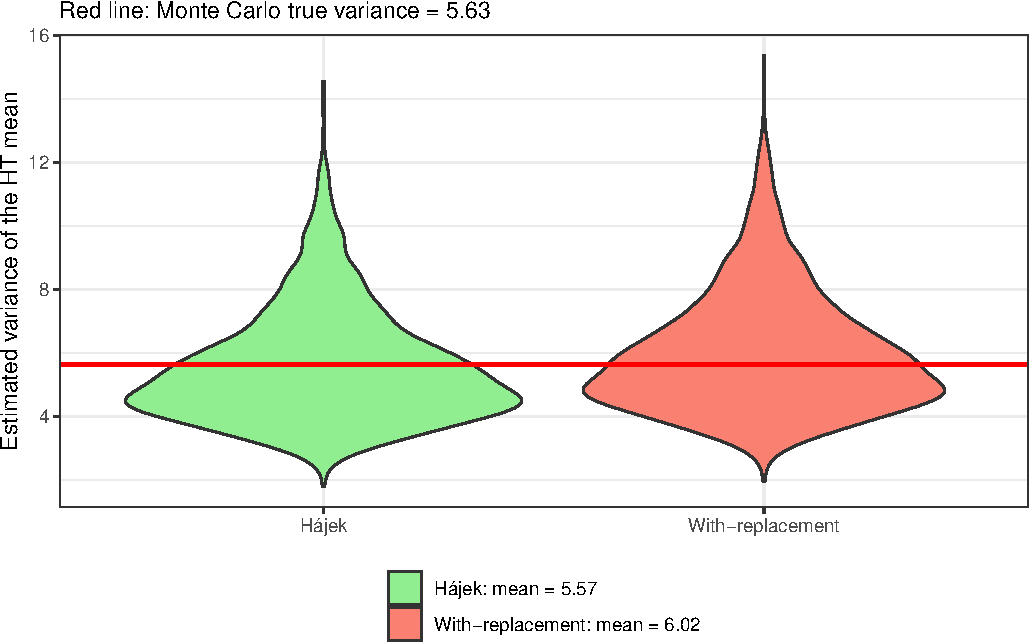
\includegraphics[keepaspectratio]{ups_files/figure-pdf/fig-wo-variances-1.pdf}}

}

\caption{\label{fig-wo-variances}Estimated variances of the HT mean in
2000 repeated samples: Hájek and with-replacement approximations. The
red line is the Monte Carlo estimate of the true variance, the variance
of the 2000 HT estimates.}

\end{figure}%

\begin{figure}

\centering{

\pandocbounded{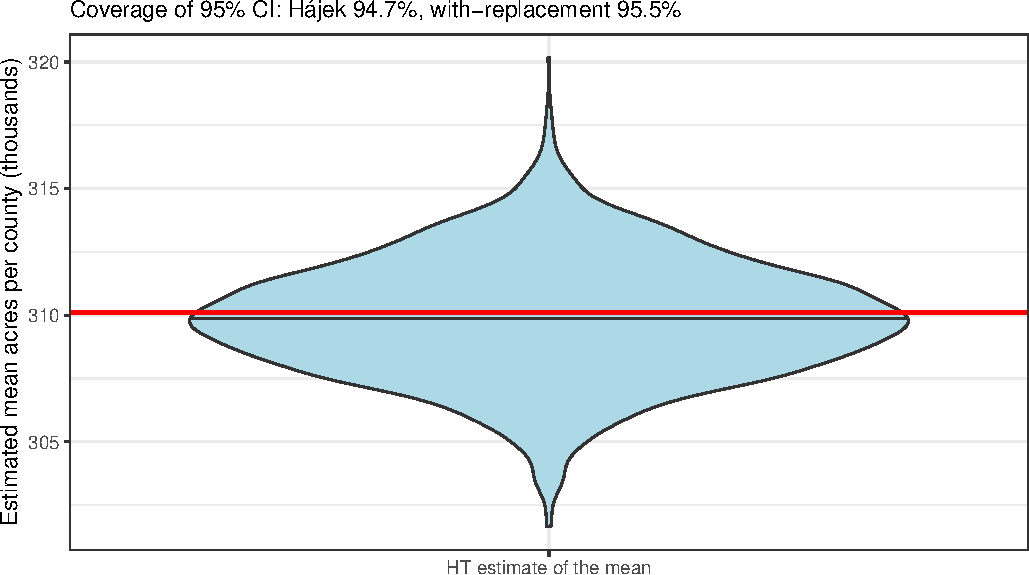
\includegraphics[keepaspectratio]{ups_files/figure-pdf/fig-wo-mean-1.pdf}}

}

\caption{\label{fig-wo-mean}HT estimates of the mean acres per county in
2000 repeated samples. The red line is the true mean; the coverage rates
of the 95\% confidence intervals with the Hájek and the with-replacement
variance estimates are given in the subtitle.}

\end{figure}%

{

\begin{longtable}[]{@{}lrr@{}}

\caption{\label{tbl-wo-summary}Estimates of the mean acres of farmland
in 1992 per county from one sample of 100 counties drawn without
replacement}

\tabularnewline

\toprule\noalign{}
Method & Estimate & Estimated SE \\
\midrule\noalign{}
\endhead
\bottomrule\noalign{}
\endlastfoot
Sample mean (ignores \(\pi_i\)) & 834.3 & 100.53 \\
HT, Hájek variance & 315.8 & 1.98 \\
HT, with-replacement variance & 315.8 & 2.06 \\

\end{longtable}

}

\textbf{Output Note:} The true mean is 310.1 thousand acres per county.
The plain sample mean, 834.3, is far off because it gives every sampled
county the same weight, although the large counties had a larger chance
of being selected; the HT estimate 315.8 corrects for that. The Hájek
and with-replacement SEs are 1.98 and 2.06. Over the 2000 repeated
samples the true standard error of the HT mean is 2.37, and the average
estimated SEs are 2.33 for the Hájek approximation and 2.43 for the
with-replacement approximation, which is a little too large, as
expected. The violin plots show the whole distribution of the two
estimated variances, with the true variance (the variance of the 2000 HT
estimates) as a red line: both are centred close to it, the
with-replacement one slightly above. The HT estimates of the mean are
centred at the true mean, as unbiasedness implies. The 95\% confidence
intervals, estimate \(\pm\) \(t_{n-1}\) SE, cover the true mean in
94.7\% of the samples with the Hájek variance and in 95.5\% with the
with-replacement variance; the latter is a little above the nominal 95\%
because its variance is too large. The ratio of the total acres in 1992
to that in 1987 is
\(\hat{B}_{\mathrm{HT}}=\hat{t}_{\mathrm{HT}}/t_x=0.998\) (SE 0.006,
Hájek).

\section{When to Use Unequal Probability Sampling}\label{sec-ups-when}

\begin{tcolorbox}[enhanced jigsaw, arc=.35mm, bottomrule=.15mm, bottomtitle=1mm, breakable, colback=white, colbacktitle=quarto-callout-warning-color!10!white, colframe=quarto-callout-warning-color-frame, coltitle=black, left=2mm, leftrule=.75mm, opacityback=0, opacitybacktitle=0.6, rightrule=.15mm, title=\textcolor{quarto-callout-warning-color}{\faExclamationTriangle}\hspace{0.5em}{Remark: UPS is risky unless y is tied to the size variable}, titlerule=0mm, toprule=.15mm, toptitle=1mm]

The gain from unequal probability sampling depends entirely on how close
the ratios \(b_i=y_i/x_i\) are to a constant, that is, on \(y_i\) being
roughly proportional to the size variable \(x_i\) used for \(\psi_i\) or
\(\pi_i\). Then the variance in Table~\ref{tbl-ups-compare} is small, as
for the county acreages. Otherwise,

\begin{itemize}
\tightlist
\item
  the estimate can be \textbf{much worse than a plain SRS average}, as
  in the second population of Section~\ref{sec-ups-toy}, where the sales
  are unrelated to the floor area;
\item
  a unit with a small \(x_i\) but a large \(y_i\) gets a very large
  weight \(1/\psi_i\) (or \(1/\pi_i\)) when it is selected, so the
  estimates are unstable, and the sample variance of the \(b_j^*\) that
  estimates the SE tends to be too small, so that the intervals
  under-cover.
\end{itemize}

UPS is therefore used mostly when the size is a good proxy of what is
measured: selecting the clusters of a multi-stage survey with
probabilities proportional to their number of households or students,
auditing by the monetary value of the items, or surveying establishments
by their employment. When the size is only loosely related to \(y_i\),
use simple random or stratified sampling, with a ratio or regression
estimator if \(x_i\) is known, which is much safer than using \(x_i\) at
the design stage.

\end{tcolorbox}

\cleardoublepage
\phantomsection
\addcontentsline{toc}{part}{Appendices}
\appendix

\chapter{List of Important Formulas}\label{sec-formulas}

This appendix collects the boxed formulas of the chapters, together with
the few companion formulas they rely on, sorted by topic. Each topic
starts with its notation; the link after each formula leads to the
section where it is derived. All designs draw units \textbf{without
replacement} unless stated otherwise (UPSWR draws with replacement).

\section{General Notation}\label{general-notation}

{\def\LTcaptype{none} % do not increment counter
\begin{longtable}[]{@{}
  >{\raggedright\arraybackslash}p{(\linewidth - 2\tabcolsep) * \real{0.5000}}
  >{\raggedright\arraybackslash}p{(\linewidth - 2\tabcolsep) * \real{0.5000}}@{}}
\toprule\noalign{}
\begin{minipage}[b]{\linewidth}\raggedright
Symbol
\end{minipage} & \begin{minipage}[b]{\linewidth}\raggedright
Meaning
\end{minipage} \\
\midrule\noalign{}
\endhead
\bottomrule\noalign{}
\endlastfoot
\(N\), \(n\) & number of units in the population \(\mathcal U\) and in
the sample \(\mathcal S\) \\
\(y_i\) & value of the study variable for unit \(i\) \\
\(t = \sum_{i=1}^N y_i\), \(\ \bar y_U = t/N\) & population total and
population mean \\
\(S^2 = \frac{1}{N-1}\sum_{i=1}^N (y_i-\bar y_U)^2\) & population
variance \\
\(\bar y = \frac1n\sum_{i\in\mathcal S} y_i\),
\(\ s^2 = \frac{1}{n-1}\sum_{i\in\mathcal S}(y_i-\bar y)^2\) & sample
mean and sample variance \\
\(1 - n/N\) & finite population correction (fpc) \\
\(\hat V(\cdot)\), \(\ \mathrm{SE}(\cdot) = \sqrt{\hat V(\cdot)}\) &
estimated variance and standard error \\
\(z_{\alpha/2}\), \(\ t_{\alpha/2,\,df}\) & upper \(\alpha/2\) quantiles
of the standard normal and the \(t\) distribution \\
\end{longtable}
}

\textbf{Confidence interval.} For any estimator \(\hat\theta\) in this
list, an approximate \(100(1-\alpha)\%\) confidence interval is \[
\boxed{\hat\theta \pm t_{\alpha/2,\,df}\,\mathrm{SE}(\hat\theta)}
\] with \(df = n-1\) for an SRS (\(n - H\) for \(H\) strata); for large
samples \(z_{\alpha/2}\) may replace \(t_{\alpha/2,\,df}\)
(Section~\ref{sec-srs-ci}).

\section{Simple Random Sampling}\label{simple-random-sampling-1}

\emph{Notation:} \(\hat p\) is the sample proportion of a 0/1 variable;
\(e\) is the margin of error.

\textbf{Mean} (Section~\ref{sec-srs-formulas}): \[
\boxed{
\hat{V}(\bar{y}) = \left(1 - \frac{n}{N}\right)\frac{s^2}{n}, \qquad
\mathrm{SE}(\bar y) = \sqrt{\Big(1-\frac nN\Big)\frac{s^2}{n}}}
\]

\textbf{Total} (Section~\ref{sec-srs-formulas}): \[
\boxed{
\hat{t} = N\bar{y}, \qquad
\hat{V}(\hat{t}) = N^2\left(1 - \frac{n}{N}\right)\frac{s^2}{n}, \qquad
\mathrm{SE}(\hat{t}) = N\,\mathrm{SE}(\bar{y})}
\]

\textbf{Proportion} (Section~\ref{sec-srs-formulas}); the number of
units with the characteristic is estimated by \(N\hat p\) with SE
\(N\,\mathrm{SE}(\hat p)\): \[
\boxed{\hat V(\hat p) = \Big(1-\frac nN\Big)\frac{\hat p (1-\hat p)}{n-1}}
\]

\textbf{Sample size} for margin of error \(e\) at level \(1-\alpha\),
with \(n_0 = (z_{\alpha/2}S/e)^2\) (Section~\ref{sec-srs-sample-size}):
\[
\boxed{n = \frac{n_0}{1+n_0/N} = \frac{z_{\alpha/2}^2 S^2}{e^2 + z_{\alpha/2}^2 S^2/N}}
\]

\section{Stratified Random Sampling}\label{stratified-random-sampling-1}

\emph{Notation:} stratum \(h = 1,\ldots,H\) has \(N_h\) units, of which
\(n_h\) are sampled by SRS; \(\pi_h = N_h/N\) is the stratum weight;
\(\overline y_h\), \(s_h^2\) and \(\hat p_h\) are the sample mean,
variance and proportion in stratum \(h\); \(S_h^2\) is the population
variance in stratum \(h\); \(c_h\) is the cost of sampling one unit in
stratum \(h\).

\textbf{Estimators of the total and the mean}
(Section~\ref{sec-strata-estimation}): \[
\boxed{
\hat t_{\text{str}} = \sum_{h=1}^H N_h \overline y_h,
\qquad
\overline y_{\text{str}} = \frac{\hat t_{\text{str}}}{N} = \sum_{h=1}^H \pi_h\overline y_h}
\]

\textbf{Variance and SE} (\(v_h\) is the contribution of stratum \(h\);
\(\hat V(\hat t_{\text{str}}) = N^2\hat V(\overline y_{\text{str}})\))
(Section~\ref{sec-strata-estimation}): \[
\boxed{
\hat V(\overline y_{\text{str}}) = \sum_{h=1}^H v_h, \qquad
v_h = \Big(1-\frac{n_h}{N_h}\Big)\pi_h^2\frac{s_h^2}{n_h}, \qquad
\mathrm{SE}(\overline y_{\text{str}}) = \sqrt{\hat V(\overline y_{\text{str}})}}
\]

\textbf{Proportion} (Section~\ref{sec-strata-proportions}): \[
\boxed{\begin{aligned}
\hat p_{\text{str}} &= \sum_{h=1}^H \frac{N_h}{N}\hat p_h, \\
\hat V(\hat p_{\text{str}}) &= \sum_{h=1}^H \Big(1-\frac{n_h}{N_h}\Big)\Big(\frac{N_h}{N}\Big)^2\frac{\hat p_h(1-\hat p_h)}{n_h-1}
\end{aligned}}
\]

\textbf{Proportional allocation} \(n_h = n\pi_h\)
(Section~\ref{sec-strata-prop}): \[
\boxed{V_{\text{prop}}(\overline y_{\text{str}}) = \left(1 - \frac{n}{N}\right)\frac{1}{n}\sum_{h=1}^H \pi_h S_h^2}
\]

\textbf{Gain over SRS} under proportional allocation; SSB and SSTO are
the between-strata and total sums of squares of the population
(Section~\ref{sec-strata-prop}): \[
\boxed{\text{percentage of variance reduction} \approx \frac{\text{SSB}}{\text{SSTO}} = R^2_{y\mid\text{strata}}}
\]

\textbf{Optimal allocation} for a fixed cost
(Section~\ref{sec-strata-optimal}): \[
\boxed{
n_h = \left(\frac{N_hS_h/\sqrt{c_h}}{\sum_{l=1}^H N_lS_l/\sqrt{c_l}}\right)n,
\qquad n_h \propto \frac{N_hS_h}{\sqrt{c_h}}}
\]

\textbf{Neyman allocation} (equal costs \(c_h\)) and its variance
(Section~\ref{sec-strata-optimal}): \[
\boxed{n_h = n \frac{N_h S_h}{\sum_{l=1}^H N_l S_l}}, \qquad
\boxed{V_{\text{opt}}(\overline{y}_{\text{str}}) = \frac{1}{n}\left(\sum_{h=1}^H \pi_h S_h\right)^2 - \frac{1}{N}\sum_{h=1}^H \pi_h S_h^2}
\]

\section{Ratio and Regression
Estimation}\label{ratio-and-regression-estimation-1}

\emph{Notation:} SRS of \(n\) pairs \((x_i, y_i)\); the auxiliary
variable \(x\) has known population total \(t_x\) and mean
\(\bar x_U = t_x/N\); \(\bar x\), \(\bar y\) are the sample means;
\(\hat t_y = N\bar y\), \(\hat t_x = N\bar x\).

\textbf{Ratio estimators} (Section~\ref{sec-ratio-theory}): \[
\boxed{\hat B = \frac{\bar y}{\bar x} = \frac{\sum_{i=1}^n y_i}{\sum_{i=1}^n x_i} = \frac{\hat t_y}{\hat t_x},
\qquad
\hat t_{yr} = \hat B\, t_x = N\,\hat{\bar y}_r,
\qquad
\hat{\bar y}_r = \hat B\, \bar x_U}
\]

\textbf{Ratio variances}, with residuals \(e_i = y_i - \hat B x_i\) and
\(s_e^2 = \frac{1}{n-1}\sum_{i=1}^n e_i^2\)
(Section~\ref{sec-ratio-theory}): \[
\boxed{\begin{aligned}
\hat V(\hat B) &= \frac{1}{\bar x^2}\left(1 - \frac nN\right)\frac{s_e^2}{n}, \\
\hat V(\hat{\bar y}_r) &= \bar x_U^2\,\hat V(\hat B) = \left(\frac{\bar x_U}{\bar x}\right)^2\left(1 - \frac nN\right)\frac{s_e^2}{n}, \\
\hat V(\hat t_{yr}) &= N^2\,\hat V(\hat{\bar y}_r)
\end{aligned}}
\]

\textbf{Regression estimators}, with the least-squares fit
\(\hat B_1 = \sum(x_i-\bar x)(y_i-\bar y)/\sum(x_i-\bar x)^2\) and
\(\hat B_0 = \bar y - \hat B_1\bar x\)
(Section~\ref{sec-regression-theory}): \[
\boxed{\hat{\bar y}_{reg} = \hat B_0 + \hat B_1\bar x_U = \bar y + \hat B_1\left(\bar x_U - \bar x\right),
\qquad
\hat t_{reg} = N\hat{\bar y}_{reg} = N\hat B_0 + \hat B_1 t_x}
\]

\textbf{Regression variance} (Section~\ref{sec-regression-theory}): \[
\boxed{\hat V(\hat{\bar y}_{reg}) = \left(1 - \frac nN\right)\frac{s_e^2}{n},
\qquad
s_e^2 = \frac{1}{n-2}\sum_{i=1}^n\left(y_i - \hat B_0 - \hat B_1 x_i\right)^2}
\]

\textbf{Post-stratification}: an SRS sorted afterwards into \(H\) groups
of known sizes \(N_h\), \(\pi_h = N_h/N\); \(\bar y_h\) and \(s_h^2\)
are the mean and variance of the sampled units in group \(h\), and
\(n_h^{post} = n\pi_h\) is its expected sample size
(Section~\ref{sec-poststrat-theory}): \[
\boxed{\bar y_{post} = \sum_{h=1}^H \pi_h\,\bar y_h,
\qquad
\hat t_{post} = N\bar y_{post}}
\] \[
\boxed{\hat V(\bar y_{post}) = \sum_{h=1}^H \pi_h^2\left(1 - \frac{n_h^{post}}{N_h}\right)\frac{s_h^2}{n_h^{post}}
= \left(1 - \frac nN\right)\frac1n\sum_{h=1}^H \pi_h s_h^2}
\]

\textbf{Domain mean}: the \(n_d\) sampled units \(\mathcal S_d\) that
fall in domain \(d\) have mean \(\bar y_d\)
(Section~\ref{sec-domain-theory}): \[
\boxed{\hat V(\bar y_d) = \left(1 - \frac nN\right)\frac{s_d^2}{n_d},
\qquad
s_d^2 = \frac{1}{n_d - 1}\sum_{i \in \mathcal S_d}\left(y_i - \bar y_d\right)^2}
\]

\textbf{Prediction estimator} with a fitted model
\(\hat y_i = \hat m(x_i)\) for every population unit
(Section~\ref{sec-ml-prediction}): \[
\boxed{\hat{\bar y}_{\text{pred}} = \frac1N\sum_{i=1}^N \hat y_i, \qquad
\hat t_{y,\text{pred}} = \sum_{i=1}^N \hat y_i}
\]

\section{Cluster Sampling}\label{cluster-sampling-1}

\emph{Notation:} an SRS \(\mathcal S\) of \(n\) of the \(N\) clusters
(psus); cluster \(i\) has \(M_i\) elements (ssus), total \(t_i\) and
mean \(\bar y_i\); \(M_0 = \sum_{i=1}^N M_i\);
\(\bar M = \frac1n\sum_{i\in\mathcal S}M_i\) is the average size of the
sampled clusters; \(s_t^2\) is the sample variance of the \(t_i\). In
two-stage sampling \(m_i\) of the \(M_i\) elements are subsampled, with
mean \(\bar y_i\) and variance \(s_i^2\), and
\(\hat t_i = M_i\bar y_i\).

\textbf{One stage, equal sizes} \(M_i = M\): an SRS of cluster totals
(Section~\ref{sec-cluster-equal}): \[
\boxed{\hat t = \frac Nn\sum_{i\in\mathcal S} t_i, \qquad
\mathrm{SE}(\hat t) = N\sqrt{\Big(1-\frac nN\Big)\frac{s_t^2}{n}}, \qquad
\hat{\bar y} = \frac{\hat t}{NM}}
\]

\textbf{One stage, unequal sizes: ratio estimator of the mean per
element} (Section~\ref{sec-cluster-unequal}): \[
\boxed{
\hat{\bar y}_r = \frac{\sum_{i\in\mathcal S} t_i}{\sum_{i\in\mathcal S} M_i} = \frac{\sum_{i\in\mathcal S} M_i\bar y_i}{\sum_{i\in\mathcal S} M_i}}
\] \[
\boxed{
\mathrm{SE}(\hat{\bar y}_r) = \sqrt{\Big(1-\frac nN\Big)\frac{s_e^2}{n\bar M^2}}, \qquad
s_e^2 = \frac{1}{n-1}\sum_{i\in\mathcal S}e_i^2, \qquad e_i = t_i-\hat{\bar y}_r M_i}
\]

\textbf{Two stages: ratio estimator}
(Section~\ref{sec-cluster-two-stage}): \[
\boxed{
\hat{\bar y}_r = \frac{\sum_{i\in\mathcal S}\hat t_i}{\sum_{i\in\mathcal S}M_i} = \frac{\sum_{i\in\mathcal S}M_i\bar y_i}{\sum_{i\in\mathcal S}M_i}}
\]

\textbf{Two stages: variance}, a ratio piece plus \(n/N\) times a
stratified piece, with \(e_i = \hat t_i - \hat{\bar y}_r M_i\) and
\(M = n\bar M\) (Section~\ref{sec-cluster-two-stage}): \[
\boxed{\begin{aligned}
\hat V(\hat{\bar y}_r) &= \hat V_{\text{ratio}} + \frac nN\,\hat V_{\text{str}}, \\
\hat V_{\text{ratio}} &= \Big(1-\frac nN\Big)\frac{s_e^2}{n\bar M^2}, \qquad
\hat V_{\text{str}} = \sum_{i\in\mathcal S}\Big(\frac{M_i}{M}\Big)^2\Big(1-\frac{m_i}{M_i}\Big)\frac{s_i^2}{m_i}
\end{aligned}}
\]

\section{Unequal Probability
Sampling}\label{unequal-probability-sampling-1}

\emph{Notation:} \(n\) independent draws \textbf{with replacement}
(UPSWR); on each draw, unit \(i\) is selected with probability
\(\psi_i = x_i/t_x\) for a size variable \(x_i\); the unit selected on
draw \(j\) has ratio \(b_j^* = y_j^*/x_j^*\); \(B = t/t_x\).

\textbf{Hansen--Hurwitz (HH) estimator of \(B\)}
(Section~\ref{sec-ups-hh-theory}): \[
\boxed{\hat{B}_{\mathrm{HH}}=\bar{b}^*=\frac{1}{n}\sum_{j=1}^n b_j^*}, \qquad
\boxed{\widehat{\mathrm{SE}}(\hat{B}_{\mathrm{HH}})=\frac{s_{b^*}}{\sqrt{n}}},\qquad
s_{b^*}^2=\frac{1}{n-1}\sum_{j=1}^n\left(b_j^*-\bar{b}^*\right)^2
\]

\textbf{HH mean and total}: multiply the estimate and its SE by
\(\bar x_U\) or \(t_x\) (Section~\ref{sec-ups-hh-theory}): \[
\boxed{
\hat{\bar{y}}_{\mathrm{HH}}=\bar{x}_U\,\bar{b}^*,\quad
\widehat{\mathrm{SE}}(\hat{\bar{y}}_{\mathrm{HH}})=\bar{x}_U\,\frac{s_{b^*}}{\sqrt{n}},\qquad
\hat{t}_{\mathrm{HH}}=t_x\,\bar{b}^*,\quad
\widehat{\mathrm{SE}}(\hat{t}_{\mathrm{HH}})=t_x\,\frac{s_{b^*}}{\sqrt{n}}}
\]

\textbf{One-stage cluster sampling with PPS}: \(y_i \to t_i\),
\(x_i \to M_i\), \(\psi_i = M_i/M_0\); the ratio of the cluster on draw
\(j\) is its mean per element \(\bar y_j^*\)
(Section~\ref{sec-ups-cluster-theory}): \[
\boxed{\hat{B}_{\mathrm{HH}}=\bar{b}^*=\frac{1}{n}\sum_{j=1}^n \bar{y}_j^*},\qquad
\widehat{\mathrm{SE}}(\hat{B}_{\mathrm{HH}})=\frac{s_{b^*}}{\sqrt{n}},\qquad
s_{b^*}^2=\frac{1}{n-1}\sum_{j=1}^n\left(\bar{y}_j^*-\bar{b}^*\right)^2
\]

\textbf{Two-stage cluster sampling with PPS}: \(\bar y_j^*\) is now the
mean of the \(m_j\) elements subsampled on draw \(j\); the mean per
cluster and the total are \(\bar M_U\hat B_{\mathrm{HH}}\) and
\(M_0\hat B_{\mathrm{HH}}\), with SEs scaled the same way
(Section~\ref{sec-ups-twostage-theory}): \[
\boxed{\hat{B}_{\mathrm{HH}}=\bar{y}^*=\frac{1}{n}\sum_{j=1}^n \bar{y}_j^*},\qquad
\widehat{\mathrm{SE}}(\hat{B}_{\mathrm{HH}})=\frac{s_{\bar{y}^*}}{\sqrt{n}},\qquad
s_{\bar{y}^*}^2=\frac{1}{n-1}\sum_{j=1}^n\left(\bar{y}_j^*-\bar{y}^*\right)^2
\]

\textbf{Horvitz--Thompson (HT) estimator}: without replacement, with
inclusion probabilities \(\pi_i = P(i\in\mathcal S)\), for example
\(\pi_i = n x_i/t_x\) (Section~\ref{sec-ups-wo-theory}): \[
\boxed{\hat{t}_{\mathrm{HT}}=\sum_{i\in\mathcal{S}}\frac{y_i}{\pi_i}}
\]

\chapter{List of Figures, Tables, and
Apps}\label{list-of-figures-tables-and-apps}

A consolidated index of every numbered figure and table in the book.
Click any entry to jump to it in context.

\section{Shinylive Apps}\label{shinylive-apps}

The simulation apps have their own archive:
\href{../shinylives_sampling/index.html}{Shinylive Apps for Sampling
Survey}.

\section{List of Figures}\label{list-of-figures}

\subsection{Introduction to Sampling
Survey}\label{introduction-to-sampling-survey-1}

\begin{itemize}
\tightlist
\item
  Figure~\ref{fig-target-sampled} --- Target population, sampling frame
  population and sampled population
\item
  Figure~\ref{fig-intro-srs} --- A simple random sample
\item
  Figure~\ref{fig-intro-stratified} --- A stratified random sample
\item
  Figure~\ref{fig-intro-cluster} --- A cluster sample
\item
  Figure~\ref{fig-intro-ratio} --- Ratio estimation: an SRS, the fitted
  line and the predicted values
\item
  Figure~\ref{fig-intro-ups} --- Unequal probability sampling with
  probabilities roughly proportional to y
\item
  Figure~\ref{fig-intro-sampdist} --- Sampling distribution of the
  sample mean under an unequal-probability design
\item
  Figure~\ref{fig-archers} --- Unbiased, precise and accurate estimators
  as archers
\end{itemize}

\subsection{Data Analysis with R}\label{data-analysis-with-r-1}

\begin{itemize}
\tightlist
\item
  Figure~\ref{fig-agpop-acres92-hist} --- Histogram of 1992 farm acreage
\item
  Figure~\ref{fig-agpop-acres-scatter} --- 1992 vs.~1987 farm acreage,
  with the 1:1 line
\item
  Figure~\ref{fig-agpop-scatter-highres} --- The saved high-resolution
  PNG, re-inserted
\item
  Figure~\ref{fig-log-acres-hist} --- Distribution of log(acres92):
  histogram with empirical density and normal fit
\end{itemize}

\subsection{Simple Random Sampling}\label{simple-random-sampling-2}

\begin{itemize}
\tightlist
\item
  Figure~\ref{fig-srs-design} --- A simple random sample from a
  synthetic population
\item
  Figure~\ref{fig-agsrs-acres92-hist} --- Farm acreage in 1992 for the
  SRS of 300 counties, with mean and median
\item
  Figure~\ref{fig-srs-simulation-distribution} --- Population
  distribution and sampling distribution of the SRS sample mean over
  5000 repeated samples (n = 300)
\item
  Figure~\ref{fig-srs-coverage-intervals} --- First 100 simulated 95\%
  confidence intervals for the SRS sample mean, with coverage failures
  highlighted
\end{itemize}

\subsection{strata}\label{strata}

\begin{itemize}
\tightlist
\item
  Figure~\ref{fig-strata-pop} --- A stratified random sample from a
  synthetic population
\item
  Figure~\ref{fig-caribou-strata} --- The six caribou strata and their
  sampled units
\item
  Figure~\ref{fig-ssb-ssw} --- Prediction by the overall mean (SSTO)
  vs.~by the stratum means (SSW)
\item
  Figure~\ref{fig-r2-compare} --- Strata with large vs.~small \(R^2\)
\item
  Figure~\ref{fig-p1mp} --- The variance \(p(1-p)\) of a 0/1 variable
\item
  Figure~\ref{fig-auxiliary} --- Strata formed by cutting an auxiliary
  variable
\item
  Figure~\ref{fig-agpop-region-boxplot} --- 1992 farm acreage by region
  stratum
\item
  Figure~\ref{fig-agpop-region-compare-boxplot} --- Sampling
  distribution of the mean under SRS, proportional, and Neyman
  allocation (region strata, 2000 simulations)
\item
  Figure~\ref{fig-agpop-acres82-boxplot} --- 1992 farm acreage by
  acres82 quantile stratum
\item
  Figure~\ref{fig-agpop-acres82-compare-boxplot} --- Sampling
  distribution of the mean under SRS, proportional, and Neyman
  allocation (acres82 strata, 2000 simulations)
\end{itemize}

\subsection{ratio}\label{ratio}

\begin{itemize}
\tightlist
\item
  Figure~\ref{fig-ratio-concept} --- Illustration of the benefits of
  ratio estimation
\item
  Figure~\ref{fig-france-toy} --- The toy France example with the ratio
  line and residuals
\item
  Figure~\ref{fig-agsrs-acres8792} --- 1992 vs.~1987 farm acreage for
  the SRS of 300 counties, with the ratio line
\item
  Figure~\ref{fig-ratio-vs-reg} --- Data suited to ratio estimation
  versus regression estimation
\item
  Figure~\ref{fig-reg-concept} --- Illustration of the benefits of
  regression estimation
\item
  Figure~\ref{fig-poststrat-concept} --- Illustration of the benefits of
  post-stratification
\item
  Figure~\ref{fig-ml-concept} --- A prediction estimator with a flexible
  (loess) model
\item
  Figure~\ref{fig-cherry-volume-diameter} --- Cherry tree volume
  vs.~diameter
\item
  Figure~\ref{fig-cherry-ratio-fit} --- Cherry tree volume vs.~diameter
  with the fitted ratio line
\item
  Figure~\ref{fig-agpop-acres8792-ratio-line} --- 1992 vs.~1987 county
  acreage with the true ratio line
\item
  Figure~\ref{fig-agpop-ratio-simulation-boxplot} --- Estimator variance
  under repeated sampling: SRS vs.~ratio estimator (2000 simulations)
\item
  Figure~\ref{fig-cherry-regression-fit} --- Cherry tree volume
  vs.~diameter with the fitted regression line
\item
  Figure~\ref{fig-deadtrees-regression-fit} --- Field counts vs.~photo
  counts of dead trees with the fitted regression line
\end{itemize}

\subsection{cluster}\label{cluster}

\begin{itemize}
\tightlist
\item
  Figure~\ref{fig-cluster-design} --- A two-stage cluster sample from a
  synthetic population
\item
  Figure~\ref{fig-cluster-vs-strat} --- Stratified sampling versus
  one-stage cluster sampling on the same population
\item
  Figure~\ref{fig-cluster-cells} --- Notation for cluster sampling:
  cells y\_ij, psu totals t\_i and sizes M\_i
\item
  Figure~\ref{fig-cluster-cells-sample} --- A two-stage cluster sample
  in the cell notation
\item
  Figure~\ref{fig-cluster-r2} --- Large versus small adjusted R² between
  clusters
\item
  Figure~\ref{fig-cluster-ratio} --- Cluster totals against cluster
  sizes, with the ratio line
\item
  Figure~\ref{fig-coots-volume} --- Coot egg volumes by clutch
\end{itemize}

\subsection{ups}\label{ups}

\begin{itemize}
\tightlist
\item
  Figure~\ref{fig-statepop-phys-vs-popn} --- Physicians vs.~population
  (log-log scale), sample of U.S. counties
\item
  Figure~\ref{fig-upswr-sim-comparison} --- Estimator distribution:
  naive SRS vs.~SRS ratio vs.~SRS regression vs.~UPSWR (2000
  simulations)
\end{itemize}

\section{List of Tables}\label{list-of-tables}

\subsection{Data Analysis with R}\label{data-analysis-with-r-2}

\begin{itemize}
\tightlist
\item
  Table~\ref{tbl-region-summary-by-statistic} --- Regional summary of
  five variables, grouped by statistic
\item
  Table~\ref{tbl-region-summary-by-variable} --- Regional summary of
  five variables, grouped by variable
\item
  Table~\ref{tbl-gtsummary-region} --- Automatic descriptive summary of
  agpop variables by region
\item
  Table~\ref{tbl-means-custom-vs-builtin} --- Comparing column means:
  custom function vs.~base R colMeans()
\end{itemize}

\subsection{strata}\label{strata-1}

\begin{itemize}
\tightlist
\item
  Table~\ref{tbl-agstrat-sample-data} --- Sample survey data for
  agstrat.csv, including stratum and weight
\item
  Table~\ref{tbl-agstrat-summary-by-region} --- Sample summary
  statistics for acres92 by region stratum
\item
  Table~\ref{tbl-seals-neyman-allocation} --- Neyman-optimal allocation
  proportions for the seals survey zones
\item
  Table~\ref{tbl-agpop-region-neyman-allocation} --- Population sizes
  and Neyman-optimal sample sizes by region stratum
\item
  Table~\ref{tbl-agpop-region-compare-methods} --- Simulated mean,
  variance, and variance reduction by allocation method (region strata)
\item
  Table~\ref{tbl-agpop-acres82-compare-methods} --- Simulated mean,
  variance, and variance reduction by allocation method (acres82 strata)
\end{itemize}

\subsection{ratio}\label{ratio-1}

\begin{itemize}
\tightlist
\item
  Table~\ref{tbl-cherry-sample-data} --- Sample data: cherry tree volume
  and diameter
\item
  Table~\ref{tbl-agpop-ratio-variance-reduction} --- Simulated variance
  and variance reduction: ratio estimator vs.
\item
  Table~\ref{tbl-agsrs-poststrat-summary} --- Observed vs.~population
  stratum proportions and post-stratified sample sizes
\end{itemize}

\subsection{cluster}\label{cluster-1}

\begin{itemize}
\tightlist
\item
  Table~\ref{tbl-algebra-raw-data} --- Raw data: algebra classes
  (sample)
\item
  Table~\ref{tbl-coots-raw-data} --- Raw data: coot egg clutches
  (sample)
\item
  Table~\ref{tbl-agpop-cluster-summary} --- Cluster-level summaries for
  the 10 sampled states
\end{itemize}

\subsection{ups}\label{ups-1}

\begin{itemize}
\tightlist
\item
  Table~\ref{tbl-statepop-sample-data} --- Sample of U.S. county
  population and physician counts
\end{itemize}

\chapter{Estimating Functions Source
Code}\label{sec-estimating-functions}

The R functions used throughout this book to compute point estimates,
standard errors, and confidence intervals --- along with their
\texttt{gt}-table formatting helpers --- are defined in a single shared
file, \texttt{samplingestimate.r}, which every chapter sources. Its full
source is listed below for reference.

\begin{Shaded}
\begin{Highlighting}[]
\CommentTok{\# =============================================================}
\CommentTok{\# Shared estimation functions for the Elements of Sampling Survey}
\CommentTok{\# book. Source this file from any chapter that needs point/SE/CI}
\CommentTok{\# estimators or their gt{-}table formatting helpers, e.g.:}
\CommentTok{\#}
\CommentTok{\#   source("samplingestimate.r")}
\CommentTok{\#}
\CommentTok{\# =============================================================}

\FunctionTok{suppressPackageStartupMessages}\NormalTok{(\{}
    \FunctionTok{library}\NormalTok{(gt)}
\NormalTok{\})}

\CommentTok{\# {-}{-}{-}{-}{-}{-}{-}{-}{-}{-}{-}{-}{-}{-}{-}{-}{-}{-}{-}{-}{-}{-}{-}{-}{-}{-}{-}{-}{-}{-}{-}{-}{-}{-}{-}{-}{-}{-}{-}{-}{-}{-}{-}{-}{-}{-}{-}{-}{-}{-}{-}{-}{-}{-}{-}{-}{-}}
\CommentTok{\# Shared gt{-}table helpers}
\CommentTok{\# {-}{-}{-}{-}{-}{-}{-}{-}{-}{-}{-}{-}{-}{-}{-}{-}{-}{-}{-}{-}{-}{-}{-}{-}{-}{-}{-}{-}{-}{-}{-}{-}{-}{-}{-}{-}{-}{-}{-}{-}{-}{-}{-}{-}{-}{-}{-}{-}{-}{-}{-}{-}{-}{-}{-}{-}{-}}

\DocumentationTok{\#\# Formats a gt table column as ordinary fixed{-}point, UNLESS its values are}
\DocumentationTok{\#\# too small (\textless{} \textasciigrave{}small\textasciigrave{} in absolute value) or too large (\textgreater{}= \textasciigrave{}large\textasciigrave{}), in}
\DocumentationTok{\#\# which case it switches that column to scientific notation (rendered as}
\DocumentationTok{\#\# "m x 10\^{}n" via gt\textquotesingle{}s exp\_style = "x10n") instead.}
\NormalTok{fmt\_auto }\OtherTok{\textless{}{-}} \ControlFlowTok{function}\NormalTok{ (gt\_tbl, data, columns, }\AttributeTok{decimals =} \DecValTok{2}\NormalTok{, }\AttributeTok{small =} \FloatTok{1e{-}3}\NormalTok{, }\AttributeTok{large =} \FloatTok{1e5}\NormalTok{)}
\NormalTok{\{}
    \ControlFlowTok{for}\NormalTok{ (col }\ControlFlowTok{in}\NormalTok{ columns)}
\NormalTok{    \{}
\NormalTok{        x }\OtherTok{\textless{}{-}}\NormalTok{ data[[col]]}
\NormalTok{        x }\OtherTok{\textless{}{-}}\NormalTok{ x[}\FunctionTok{is.finite}\NormalTok{ (x) }\SpecialCharTok{\&}\NormalTok{ x }\SpecialCharTok{!=} \DecValTok{0}\NormalTok{]}
        \ControlFlowTok{if}\NormalTok{ (}\FunctionTok{length}\NormalTok{ (x) }\SpecialCharTok{==} \DecValTok{0}\NormalTok{) }\ControlFlowTok{next}
        \DocumentationTok{\#\# judge by the column\textquotesingle{}s TYPICAL magnitude, not by its extremes: the}
        \DocumentationTok{\#\# Sum row is n times the size of a data row, and one residual that}
        \DocumentationTok{\#\# lands near zero should not push a whole column into scientific}
\NormalTok{        typical }\OtherTok{\textless{}{-}}\NormalTok{ stats}\SpecialCharTok{::}\FunctionTok{median}\NormalTok{ (}\FunctionTok{abs}\NormalTok{ (x))}
        \ControlFlowTok{if}\NormalTok{ (typical }\SpecialCharTok{\textless{}}\NormalTok{ small }\SpecialCharTok{||}\NormalTok{ typical }\SpecialCharTok{\textgreater{}=}\NormalTok{ large)}
\NormalTok{            gt\_tbl }\OtherTok{\textless{}{-}} \FunctionTok{fmt\_scientific}\NormalTok{ (gt\_tbl, }\AttributeTok{columns =}\NormalTok{ tidyselect}\SpecialCharTok{::}\FunctionTok{all\_of}\NormalTok{ (col), }\AttributeTok{decimals =}\NormalTok{ decimals, }\AttributeTok{exp\_style =} \StringTok{"x10n"}\NormalTok{)}
        \ControlFlowTok{else}
\NormalTok{            gt\_tbl }\OtherTok{\textless{}{-}} \FunctionTok{fmt\_number}\NormalTok{ (gt\_tbl, }\AttributeTok{columns =}\NormalTok{ tidyselect}\SpecialCharTok{::}\FunctionTok{all\_of}\NormalTok{ (col), }\AttributeTok{decimals =}\NormalTok{ decimals)}
\NormalTok{    \}}
\NormalTok{    gt\_tbl}
\NormalTok{\}}

\DocumentationTok{\#\# Formats a single scalar for inline formula display (fixed{-}point with}
\DocumentationTok{\#\# thousands separators, switching to "m \textbackslash{}times 10\^{}\{n\}" LaTeX scientific}
\DocumentationTok{\#\# notation for very small or very large magnitudes, mirroring fmt\_auto()\textquotesingle{}s}
\DocumentationTok{\#\# use of exp\_style = "x10n") {-}{-}{-} used to show worked{-}example steps such as}
\DocumentationTok{\#\# \textbackslash{}bar y = sum/n with the actual numbers plugged in.}
\NormalTok{fmt\_num }\OtherTok{\textless{}{-}} \ControlFlowTok{function}\NormalTok{ (x, }\AttributeTok{decimals =} \DecValTok{2}\NormalTok{, }\AttributeTok{small =} \FloatTok{1e{-}3}\NormalTok{, }\AttributeTok{large =} \FloatTok{1e5}\NormalTok{)}
\NormalTok{\{}
\NormalTok{    use\_sci }\OtherTok{\textless{}{-}} \FunctionTok{is.finite}\NormalTok{ (x) }\SpecialCharTok{\&}\NormalTok{ x }\SpecialCharTok{!=} \DecValTok{0} \SpecialCharTok{\&}\NormalTok{ (}\FunctionTok{abs}\NormalTok{ (x) }\SpecialCharTok{\textless{}}\NormalTok{ small }\SpecialCharTok{|} \FunctionTok{abs}\NormalTok{ (x) }\SpecialCharTok{\textgreater{}=}\NormalTok{ large)}
\NormalTok{    exps    }\OtherTok{\textless{}{-}} \FunctionTok{ifelse}\NormalTok{ (x }\SpecialCharTok{==} \DecValTok{0}\NormalTok{, }\DecValTok{0}\NormalTok{, }\FunctionTok{floor}\NormalTok{ (}\FunctionTok{log10}\NormalTok{ (}\FunctionTok{abs}\NormalTok{ (x))))}
\NormalTok{    mant    }\OtherTok{\textless{}{-}} \FunctionTok{ifelse}\NormalTok{ (x }\SpecialCharTok{==} \DecValTok{0}\NormalTok{, }\DecValTok{0}\NormalTok{, x }\SpecialCharTok{/} \DecValTok{10}\SpecialCharTok{\^{}}\NormalTok{exps)}
    \FunctionTok{ifelse}\NormalTok{ (use\_sci,}
            \FunctionTok{sprintf}\NormalTok{ (}\StringTok{"\%s }\SpecialCharTok{\textbackslash{}\textbackslash{}}\StringTok{times 10\^{}\{\%d\}"}\NormalTok{, }\FunctionTok{formatC}\NormalTok{ (mant, }\AttributeTok{format =} \StringTok{"f"}\NormalTok{, }\AttributeTok{digits =}\NormalTok{ decimals), exps),}
            \FunctionTok{formatC}\NormalTok{ (x, }\AttributeTok{format =} \StringTok{"f"}\NormalTok{, }\AttributeTok{digits =}\NormalTok{ decimals, }\AttributeTok{big.mark =} \StringTok{","}\NormalTok{))}
\NormalTok{\}}

\DocumentationTok{\#\# The agriculture files (agpop.csv and the samples drawn from it: agsrs.csv,}
\DocumentationTok{\#\# agstrat.csv, ...) record county acreages in acres, which run into the}
\DocumentationTok{\#\# millions and make every working table below hard to read. This converts the}
\DocumentationTok{\#\# acreage columns to THOUSANDS of acres, so a mean reads as 297.9 rather than}
\DocumentationTok{\#\# 297,897, and a variance as 2.0e5 rather than 2.0e11. The file\textquotesingle{}s missing{-}value}
\DocumentationTok{\#\# code, {-}99, becomes NA first, so it cannot be silently rescaled to {-}0.099.}
\DocumentationTok{\#\# d {-}{-}{-} data frame just read from one of those files}
\DocumentationTok{\#\# cols {-}{-}{-} acreage columns to convert (those absent from d are ignored)}
\NormalTok{acres\_in\_thousands }\OtherTok{\textless{}{-}} \ControlFlowTok{function}\NormalTok{ (d, }\AttributeTok{cols =} \FunctionTok{c}\NormalTok{ (}\StringTok{"acres92"}\NormalTok{, }\StringTok{"acres87"}\NormalTok{, }\StringTok{"acres82"}\NormalTok{))}
\NormalTok{\{}
\NormalTok{    cols }\OtherTok{\textless{}{-}} \FunctionTok{intersect}\NormalTok{ (cols, }\FunctionTok{names}\NormalTok{ (d))}
\NormalTok{    d[cols] }\OtherTok{\textless{}{-}} \FunctionTok{lapply}\NormalTok{ (d[cols], }\ControlFlowTok{function}\NormalTok{ (x) \{ x[x }\SpecialCharTok{==} \SpecialCharTok{{-}}\DecValTok{99}\NormalTok{] }\OtherTok{\textless{}{-}} \ConstantTok{NA}\NormalTok{; x }\SpecialCharTok{/} \DecValTok{1000}\NormalTok{ \})}
\NormalTok{    d}
\NormalTok{\}}

\DocumentationTok{\#\# Truncates a row{-}level working data.frame whose LAST row is a summary row}
\DocumentationTok{\#\# (e.g. "Sum"/"Total"): if there are more than head\_n data rows (excluding}
\DocumentationTok{\#\# that summary row), keeps only the first head\_n data rows, inserts one}
\DocumentationTok{\#\# "..." placeholder row, then the summary row {-}{-}{-} so long working tables}
\DocumentationTok{\#\# stay readable. id\_col {-}{-}{-} name of the row{-}label column.}
\NormalTok{truncate\_working }\OtherTok{\textless{}{-}} \ControlFlowTok{function}\NormalTok{ (working, id\_col, }\AttributeTok{head\_n =} \DecValTok{6}\NormalTok{)}
\NormalTok{\{}
\NormalTok{    n }\OtherTok{\textless{}{-}} \FunctionTok{nrow}\NormalTok{ (working) }\SpecialCharTok{{-}} \DecValTok{1}
    \ControlFlowTok{if}\NormalTok{ (n }\SpecialCharTok{\textless{}=}\NormalTok{ head\_n }\SpecialCharTok{+} \DecValTok{1}\NormalTok{) }\FunctionTok{return}\NormalTok{ (working)}

\NormalTok{    dots }\OtherTok{\textless{}{-}}\NormalTok{ working[}\DecValTok{1}\NormalTok{, ]}
\NormalTok{    dots[}\DecValTok{1}\NormalTok{, ] }\OtherTok{\textless{}{-}} \ConstantTok{NA}
\NormalTok{    dots[}\DecValTok{1}\NormalTok{, id\_col] }\OtherTok{\textless{}{-}} \StringTok{"..."}

    \FunctionTok{rbind}\NormalTok{ (working[}\FunctionTok{seq\_len}\NormalTok{ (head\_n), ], dots, working[}\FunctionTok{nrow}\NormalTok{ (working), ])}
\NormalTok{\}}

\CommentTok{\# Helper function to format estimation outputs with appropriate mathematical headers}
\NormalTok{format\_est\_gt }\OtherTok{\textless{}{-}} \ControlFlowTok{function}\NormalTok{(est\_data, }\AttributeTok{est\_type =} \FunctionTok{c}\NormalTok{(}\StringTok{"mean"}\NormalTok{, }\StringTok{"total"}\NormalTok{, }\StringTok{"ratio"}\NormalTok{, }\StringTok{"reg\_mean"}\NormalTok{, }\StringTok{"reg\_total"}\NormalTok{, }\StringTok{"ratio\_mean"}\NormalTok{, }\StringTok{"domain\_mean"}\NormalTok{,}
                                                 \StringTok{"hh\_total"}\NormalTok{, }\StringTok{"hh\_B"}\NormalTok{, }\StringTok{"hh\_ybar"}\NormalTok{)) \{}
\NormalTok{  est\_type }\OtherTok{\textless{}{-}} \FunctionTok{match.arg}\NormalTok{(est\_type)}

\NormalTok{  sym\_map }\OtherTok{\textless{}{-}} \FunctionTok{list}\NormalTok{(}
    \StringTok{"mean"}        \OtherTok{=} \FunctionTok{c}\NormalTok{(}\AttributeTok{est =} \StringTok{"$}\SpecialCharTok{\textbackslash{}\textbackslash{}}\StringTok{bar\{y\}$"}\NormalTok{,         }\AttributeTok{se =} \StringTok{"$}\SpecialCharTok{\textbackslash{}\textbackslash{}}\StringTok{mathrm\{SE\}(}\SpecialCharTok{\textbackslash{}\textbackslash{}}\StringTok{bar\{y\})$"}\NormalTok{),}
    \StringTok{"total"}       \OtherTok{=} \FunctionTok{c}\NormalTok{(}\AttributeTok{est =} \StringTok{"$}\SpecialCharTok{\textbackslash{}\textbackslash{}}\StringTok{hat\{t\}$"}\NormalTok{,         }\AttributeTok{se =} \StringTok{"$}\SpecialCharTok{\textbackslash{}\textbackslash{}}\StringTok{mathrm\{SE\}(}\SpecialCharTok{\textbackslash{}\textbackslash{}}\StringTok{hat\{t\})$"}\NormalTok{),}
    \StringTok{"ratio"}       \OtherTok{=} \FunctionTok{c}\NormalTok{(}\AttributeTok{est =} \StringTok{"$}\SpecialCharTok{\textbackslash{}\textbackslash{}}\StringTok{hat\{B\}$"}\NormalTok{,         }\AttributeTok{se =} \StringTok{"$}\SpecialCharTok{\textbackslash{}\textbackslash{}}\StringTok{mathrm\{SE\}(}\SpecialCharTok{\textbackslash{}\textbackslash{}}\StringTok{hat\{B\})$"}\NormalTok{),}
    \StringTok{"reg\_mean"}    \OtherTok{=} \FunctionTok{c}\NormalTok{(}\AttributeTok{est =} \StringTok{"$}\SpecialCharTok{\textbackslash{}\textbackslash{}}\StringTok{bar\{y\}\_\{reg\}$"}\NormalTok{,   }\AttributeTok{se =} \StringTok{"$}\SpecialCharTok{\textbackslash{}\textbackslash{}}\StringTok{mathrm\{SE\}(}\SpecialCharTok{\textbackslash{}\textbackslash{}}\StringTok{bar\{y\}\_\{reg\})$"}\NormalTok{),}
    \StringTok{"reg\_total"}   \OtherTok{=} \FunctionTok{c}\NormalTok{(}\AttributeTok{est =} \StringTok{"$}\SpecialCharTok{\textbackslash{}\textbackslash{}}\StringTok{hat\{t\}\_\{reg\}$"}\NormalTok{,   }\AttributeTok{se =} \StringTok{"$}\SpecialCharTok{\textbackslash{}\textbackslash{}}\StringTok{mathrm\{SE\}(}\SpecialCharTok{\textbackslash{}\textbackslash{}}\StringTok{hat\{t\}\_\{reg\})$"}\NormalTok{),}
    \StringTok{"ratio\_mean"}  \OtherTok{=} \FunctionTok{c}\NormalTok{(}\AttributeTok{est =} \StringTok{"$}\SpecialCharTok{\textbackslash{}\textbackslash{}}\StringTok{bar\{y\}\_\{r\}$"}\NormalTok{,     }\AttributeTok{se =} \StringTok{"$}\SpecialCharTok{\textbackslash{}\textbackslash{}}\StringTok{mathrm\{SE\}(}\SpecialCharTok{\textbackslash{}\textbackslash{}}\StringTok{bar\{y\}\_\{r\})$"}\NormalTok{),}
    \StringTok{"domain\_mean"} \OtherTok{=} \FunctionTok{c}\NormalTok{(}\AttributeTok{est =} \StringTok{"$}\SpecialCharTok{\textbackslash{}\textbackslash{}}\StringTok{bar\{y\}\_\{d\}$"}\NormalTok{,     }\AttributeTok{se =} \StringTok{"$}\SpecialCharTok{\textbackslash{}\textbackslash{}}\StringTok{mathrm\{SE\}(}\SpecialCharTok{\textbackslash{}\textbackslash{}}\StringTok{bar\{y\}\_\{d\})$"}\NormalTok{),}
    \DocumentationTok{\#\# UPSWR (Hansen{-}Hurwitz) total}
    \StringTok{"hh\_total"}      \OtherTok{=} \FunctionTok{c}\NormalTok{(}\AttributeTok{est =} \StringTok{"$}\SpecialCharTok{\textbackslash{}\textbackslash{}}\StringTok{hat\{t\}\_\{}\SpecialCharTok{\textbackslash{}\textbackslash{}}\StringTok{mathrm\{HH\}\}$"}\NormalTok{,}
                        \AttributeTok{se  =} \StringTok{"$}\SpecialCharTok{\textbackslash{}\textbackslash{}}\StringTok{mathrm\{SE\}(}\SpecialCharTok{\textbackslash{}\textbackslash{}}\StringTok{hat\{t\}\_\{}\SpecialCharTok{\textbackslash{}\textbackslash{}}\StringTok{mathrm\{HH\}\})$"}\NormalTok{),}
    \DocumentationTok{\#\# UPSWR with psi\_i = x\_i / t\_x (upswr\_est): ratio B, mean of y per unit}
    \StringTok{"hh\_B"}          \OtherTok{=} \FunctionTok{c}\NormalTok{(}\AttributeTok{est =} \StringTok{"$}\SpecialCharTok{\textbackslash{}\textbackslash{}}\StringTok{hat\{B\}\_\{}\SpecialCharTok{\textbackslash{}\textbackslash{}}\StringTok{mathrm\{HH\}\}$"}\NormalTok{,}
                        \AttributeTok{se  =} \StringTok{"$}\SpecialCharTok{\textbackslash{}\textbackslash{}}\StringTok{mathrm\{SE\}(}\SpecialCharTok{\textbackslash{}\textbackslash{}}\StringTok{hat\{B\}\_\{}\SpecialCharTok{\textbackslash{}\textbackslash{}}\StringTok{mathrm\{HH\}\})$"}\NormalTok{),}
    \StringTok{"hh\_ybar"}       \OtherTok{=} \FunctionTok{c}\NormalTok{(}\AttributeTok{est =} \StringTok{"$}\SpecialCharTok{\textbackslash{}\textbackslash{}}\StringTok{hat\{}\SpecialCharTok{\textbackslash{}\textbackslash{}}\StringTok{bar\{y\}\}\_\{}\SpecialCharTok{\textbackslash{}\textbackslash{}}\StringTok{mathrm\{HH\}\}$"}\NormalTok{,}
                        \AttributeTok{se  =} \StringTok{"$}\SpecialCharTok{\textbackslash{}\textbackslash{}}\StringTok{mathrm\{SE\}(}\SpecialCharTok{\textbackslash{}\textbackslash{}}\StringTok{hat\{}\SpecialCharTok{\textbackslash{}\textbackslash{}}\StringTok{bar\{y\}\}\_\{}\SpecialCharTok{\textbackslash{}\textbackslash{}}\StringTok{mathrm\{HH\}\})$"}\NormalTok{)}
\NormalTok{  )}

\NormalTok{  est\_sym }\OtherTok{\textless{}{-}}\NormalTok{ sym\_map[[est\_type]][}\StringTok{"est"}\NormalTok{]}
\NormalTok{  se\_sym  }\OtherTok{\textless{}{-}}\NormalTok{ sym\_map[[est\_type]][}\StringTok{"se"}\NormalTok{]}

  \CommentTok{\# Convert to data frame. Use unname() to strip hidden lm() coefficient names}
  \ControlFlowTok{if}\NormalTok{ (}\FunctionTok{is.vector}\NormalTok{(est\_data) }\SpecialCharTok{\&\&} \SpecialCharTok{!}\FunctionTok{is.list}\NormalTok{(est\_data)) \{}
\NormalTok{    df }\OtherTok{\textless{}{-}} \FunctionTok{as.data.frame}\NormalTok{(}\FunctionTok{t}\NormalTok{(}\FunctionTok{unname}\NormalTok{(est\_data)))}
\NormalTok{  \} }\ControlFlowTok{else}\NormalTok{ \{}
\NormalTok{    df }\OtherTok{\textless{}{-}} \FunctionTok{as.data.frame}\NormalTok{(est\_data)}
\NormalTok{  \}}

  \CommentTok{\# Force standard column names so gt() never gets confused}
  \FunctionTok{colnames}\NormalTok{(df) }\OtherTok{\textless{}{-}} \FunctionTok{c}\NormalTok{(}\StringTok{"Est."}\NormalTok{, }\StringTok{"S.E."}\NormalTok{, }\StringTok{"ci.low"}\NormalTok{, }\StringTok{"ci.upp"}\NormalTok{)}

  \CommentTok{\# Check if we should use rownames as a stub}
\NormalTok{  use\_stub }\OtherTok{\textless{}{-}} \SpecialCharTok{!}\FunctionTok{is.null}\NormalTok{(}\FunctionTok{rownames}\NormalTok{(df)) }\SpecialCharTok{\&\&} \SpecialCharTok{!}\FunctionTok{all}\NormalTok{(}\FunctionTok{rownames}\NormalTok{(df) }\SpecialCharTok{==} \FunctionTok{as.character}\NormalTok{(}\DecValTok{1}\SpecialCharTok{:}\FunctionTok{nrow}\NormalTok{(df)))}

\NormalTok{  df }\SpecialCharTok{|\textgreater{}}
    \FunctionTok{gt}\NormalTok{(}\AttributeTok{rownames\_to\_stub =}\NormalTok{ use\_stub) }\SpecialCharTok{|\textgreater{}}
    \FunctionTok{cols\_label}\NormalTok{(}
      \AttributeTok{Est.   =} \FunctionTok{md}\NormalTok{(est\_sym),}
      \AttributeTok{S.E.   =} \FunctionTok{md}\NormalTok{(se\_sym),}
      \AttributeTok{ci.low =} \FunctionTok{md}\NormalTok{(}\StringTok{"95\% CI Lower"}\NormalTok{),}
      \AttributeTok{ci.upp =} \FunctionTok{md}\NormalTok{(}\StringTok{"95\% CI Upper"}\NormalTok{)}
\NormalTok{    ) }\SpecialCharTok{|\textgreater{}}
    \FunctionTok{fmt\_number}\NormalTok{(}
      \AttributeTok{columns =} \FunctionTok{everything}\NormalTok{(),}
      \AttributeTok{decimals =} \DecValTok{2}
\NormalTok{    ) }\SpecialCharTok{|\textgreater{}}
    \FunctionTok{tab\_options}\NormalTok{(}\AttributeTok{table.width =} \FunctionTok{pct}\NormalTok{(}\DecValTok{70}\NormalTok{))}
\NormalTok{\}}

\DocumentationTok{\#\# Formats an lm object as two gt tables, replacing the plain{-}text}
\DocumentationTok{\#\# summary(lmfit) output:}
\DocumentationTok{\#\#   $coef {-}{-}{-} coefficient table (Estimate, S.E., t value, p value)}
\DocumentationTok{\#\#   $fit  {-}{-}{-} one{-}row table of model fit statistics, including R\^{}2}
\DocumentationTok{\#\# returns list($coef, $fit)}
\NormalTok{format\_lm\_gt }\OtherTok{\textless{}{-}} \ControlFlowTok{function}\NormalTok{ (lmfit)}
\NormalTok{\{}
\NormalTok{    s }\OtherTok{\textless{}{-}} \FunctionTok{summary}\NormalTok{ (lmfit)}

\NormalTok{    coef\_df }\OtherTok{\textless{}{-}} \FunctionTok{as.data.frame}\NormalTok{ (s}\SpecialCharTok{$}\NormalTok{coefficients)}
    \FunctionTok{colnames}\NormalTok{ (coef\_df) }\OtherTok{\textless{}{-}} \FunctionTok{c}\NormalTok{ (}\StringTok{"Estimate"}\NormalTok{, }\StringTok{"S.E."}\NormalTok{, }\StringTok{"t value"}\NormalTok{, }\StringTok{"p value"}\NormalTok{)}

\NormalTok{    coef\_gt }\OtherTok{\textless{}{-}}\NormalTok{ coef\_df }\SpecialCharTok{|\textgreater{}}
        \FunctionTok{gt}\NormalTok{ (}\AttributeTok{rownames\_to\_stub =} \ConstantTok{TRUE}\NormalTok{) }\SpecialCharTok{|\textgreater{}}
        \FunctionTok{fmt\_number}\NormalTok{ (}\AttributeTok{columns =} \FunctionTok{c}\NormalTok{ (}\StringTok{"Estimate"}\NormalTok{, }\StringTok{"S.E."}\NormalTok{, }\StringTok{"t value"}\NormalTok{), }\AttributeTok{decimals =} \DecValTok{4}\NormalTok{) }\SpecialCharTok{|\textgreater{}}
        \FunctionTok{fmt\_number}\NormalTok{ (}\AttributeTok{columns =} \StringTok{"p value"}\NormalTok{, }\AttributeTok{decimals =} \DecValTok{4}\NormalTok{) }\SpecialCharTok{|\textgreater{}}
        \FunctionTok{tab\_header}\NormalTok{ (}\AttributeTok{title =} \StringTok{"Coefficient Estimates"}\NormalTok{) }\SpecialCharTok{|\textgreater{}}
        \FunctionTok{tab\_options}\NormalTok{ (}\AttributeTok{table.width =} \FunctionTok{pct}\NormalTok{(}\DecValTok{70}\NormalTok{))}

\NormalTok{    fstat }\OtherTok{\textless{}{-}}\NormalTok{ s}\SpecialCharTok{$}\NormalTok{fstatistic}
\NormalTok{    fit\_df }\OtherTok{\textless{}{-}} \FunctionTok{data.frame}\NormalTok{ (}
        \AttributeTok{R.squared     =}\NormalTok{ s}\SpecialCharTok{$}\NormalTok{r.squared,}
        \AttributeTok{Adj.R.squared =}\NormalTok{ s}\SpecialCharTok{$}\NormalTok{adj.r.squared,}
        \AttributeTok{Sigma         =}\NormalTok{ s}\SpecialCharTok{$}\NormalTok{sigma,}
        \AttributeTok{F.statistic   =} \FunctionTok{unname}\NormalTok{ (fstat[}\StringTok{"value"}\NormalTok{]),}
        \AttributeTok{p.value       =} \FunctionTok{unname}\NormalTok{ (}\FunctionTok{pf}\NormalTok{ (fstat[}\StringTok{"value"}\NormalTok{], fstat[}\StringTok{"numdf"}\NormalTok{], fstat[}\StringTok{"dendf"}\NormalTok{], }\AttributeTok{lower.tail =} \ConstantTok{FALSE}\NormalTok{))}
\NormalTok{    )}

\NormalTok{    fit\_gt }\OtherTok{\textless{}{-}}\NormalTok{ fit\_df }\SpecialCharTok{|\textgreater{}}
        \FunctionTok{gt}\NormalTok{ () }\SpecialCharTok{|\textgreater{}}
        \FunctionTok{cols\_label}\NormalTok{ (}
            \AttributeTok{R.squared     =} \FunctionTok{md}\NormalTok{ (}\StringTok{"$R\^{}2$"}\NormalTok{),}
            \AttributeTok{Adj.R.squared =} \FunctionTok{md}\NormalTok{ (}\StringTok{"Adj. $R\^{}2$"}\NormalTok{),}
            \AttributeTok{Sigma         =} \FunctionTok{md}\NormalTok{ (}\StringTok{"$}\SpecialCharTok{\textbackslash{}\textbackslash{}}\StringTok{hat}\SpecialCharTok{\textbackslash{}\textbackslash{}}\StringTok{sigma$"}\NormalTok{),}
            \AttributeTok{F.statistic   =} \StringTok{"F{-}statistic"}\NormalTok{,}
            \AttributeTok{p.value       =} \StringTok{"p{-}value"}
\NormalTok{        ) }\SpecialCharTok{|\textgreater{}}
        \FunctionTok{fmt\_number}\NormalTok{ (}\AttributeTok{columns =} \FunctionTok{everything}\NormalTok{ (), }\AttributeTok{decimals =} \DecValTok{4}\NormalTok{) }\SpecialCharTok{|\textgreater{}}
        \FunctionTok{tab\_header}\NormalTok{ (}\AttributeTok{title =} \StringTok{"Model Fit Summary"}\NormalTok{) }\SpecialCharTok{|\textgreater{}}
        \FunctionTok{tab\_options}\NormalTok{ (}\AttributeTok{table.width =} \FunctionTok{pct}\NormalTok{(}\DecValTok{70}\NormalTok{))}

    \FunctionTok{list}\NormalTok{ (}\AttributeTok{coef =}\NormalTok{ coef\_gt, }\AttributeTok{fit =}\NormalTok{ fit\_gt)}
\NormalTok{\}}

\CommentTok{\# {-}{-}{-}{-}{-}{-}{-}{-}{-}{-}{-}{-}{-}{-}{-}{-}{-}{-}{-}{-}{-}{-}{-}{-}{-}{-}{-}{-}{-}{-}{-}{-}{-}{-}{-}{-}{-}{-}{-}{-}{-}{-}{-}{-}{-}{-}{-}{-}{-}{-}{-}{-}{-}{-}{-}{-}{-}}
\CommentTok{\# Base Estimators}
\CommentTok{\# {-}{-}{-}{-}{-}{-}{-}{-}{-}{-}{-}{-}{-}{-}{-}{-}{-}{-}{-}{-}{-}{-}{-}{-}{-}{-}{-}{-}{-}{-}{-}{-}{-}{-}{-}{-}{-}{-}{-}{-}{-}{-}{-}{-}{-}{-}{-}{-}{-}{-}{-}{-}{-}{-}{-}{-}{-}}

\DocumentationTok{\#\# sdata {-}{-}{-} a vector of original survey data}
\DocumentationTok{\#\# N {-}{-}{-} population size}
\DocumentationTok{\#\# estimate {-}{-}{-} "mean" (default) returns the population MEAN estimate;}
\DocumentationTok{\#\#              "total" returns the population TOTAL estimate (N * mean,}
\DocumentationTok{\#\#              with SE/CI scaled accordingly); requires finite N}
\DocumentationTok{\#\# show.details {-}{-}{-} if TRUE (default), also return a gt table of the}
\DocumentationTok{\#\#                  row{-}level working values y\_i, the fitted value \textbackslash{}hat y\_i}
\DocumentationTok{\#\#                  (constant, and equal to \textbackslash{}bar y under the SRS model),}
\DocumentationTok{\#\#                  e\_i = y\_i{-}\textbackslash{}hat y\_i, and e\_i\^{}2, with a Sum row and a}
\DocumentationTok{\#\#                  footnote showing s\_y\^{}2; NULL otherwise}
\DocumentationTok{\#\# col\_labels {-}{-}{-} named list (y, yhat, dev, ybar, s) of RAW latex: the}
\DocumentationTok{\#\#                data, fitted and deviation columns, the symbol for the}
\DocumentationTok{\#\#                sample mean, and for the sample SD; a partial list fills in}
\DocumentationTok{\#\#                the remaining defaults, so callers can override just one label}
\DocumentationTok{\#\# title {-}{-}{-} the working table\textquotesingle{}s title}
\DocumentationTok{\#\# returns list ($estimate = c(Est., S.E., ci.low, ci.upp), $table)}
\NormalTok{srs\_est }\OtherTok{\textless{}{-}} \ControlFlowTok{function}\NormalTok{ (sdata, }\AttributeTok{N =} \ConstantTok{Inf}\NormalTok{, }\AttributeTok{estimate =} \FunctionTok{c}\NormalTok{ (}\StringTok{"mean"}\NormalTok{, }\StringTok{"total"}\NormalTok{),}
                      \AttributeTok{show.details =} \ConstantTok{TRUE}\NormalTok{, }\AttributeTok{col\_labels =} \FunctionTok{list}\NormalTok{ (),}
                      \AttributeTok{title =} \StringTok{"SRS Mean Estimation: Working Table"}\NormalTok{, }\AttributeTok{decimals =} \DecValTok{2}\NormalTok{)}
\NormalTok{\{}
\NormalTok{    estimate }\OtherTok{\textless{}{-}} \FunctionTok{match.arg}\NormalTok{ (estimate)}
    \DocumentationTok{\#\# show \textasciigrave{}decimals\textasciigrave{} decimals in the working table and its notes}
\NormalTok{    fmt\_num\_default }\OtherTok{\textless{}{-}}\NormalTok{ fmt\_num}
\NormalTok{    fmt\_num }\OtherTok{\textless{}{-}} \ControlFlowTok{function}\NormalTok{ (x, }\AttributeTok{d =}\NormalTok{ decimals) }\FunctionTok{fmt\_num\_default}\NormalTok{ (x, }\AttributeTok{decimals =} \ControlFlowTok{if}\NormalTok{ (d }\SpecialCharTok{==} \DecValTok{2}\NormalTok{) decimals }\ControlFlowTok{else}\NormalTok{ d)}
\NormalTok{    col\_labels }\OtherTok{\textless{}{-}} \FunctionTok{modifyList}\NormalTok{ (}\FunctionTok{list}\NormalTok{ (}\AttributeTok{y =} \StringTok{"y\_i"}\NormalTok{, }\AttributeTok{yhat =} \StringTok{"}\SpecialCharTok{\textbackslash{}\textbackslash{}}\StringTok{hat y\_i"}\NormalTok{, }\AttributeTok{dev =} \StringTok{"e\_i"}\NormalTok{,}
                                    \AttributeTok{ybar =} \StringTok{"}\SpecialCharTok{\textbackslash{}\textbackslash{}}\StringTok{bar y"}\NormalTok{, }\AttributeTok{s =} \StringTok{"s\_y"}\NormalTok{), col\_labels)}
\NormalTok{    ybar\_lab }\OtherTok{\textless{}{-}}\NormalTok{ col\_labels}\SpecialCharTok{$}\NormalTok{ybar}
\NormalTok{    s\_lab    }\OtherTok{\textless{}{-}}\NormalTok{ col\_labels}\SpecialCharTok{$}\NormalTok{s}

\NormalTok{    n }\OtherTok{\textless{}{-}} \FunctionTok{length}\NormalTok{ (sdata)}
\NormalTok{    ybar }\OtherTok{\textless{}{-}} \FunctionTok{mean}\NormalTok{ (sdata)}
\NormalTok{    dev }\OtherTok{\textless{}{-}}\NormalTok{ sdata }\SpecialCharTok{{-}}\NormalTok{ ybar}
\NormalTok{    s2y }\OtherTok{\textless{}{-}} \FunctionTok{sum}\NormalTok{ (dev}\SpecialCharTok{\^{}}\DecValTok{2}\NormalTok{) }\SpecialCharTok{/}\NormalTok{ (n }\SpecialCharTok{{-}} \DecValTok{1}\NormalTok{)}
\NormalTok{    se.ybar }\OtherTok{\textless{}{-}} \FunctionTok{sqrt}\NormalTok{((}\DecValTok{1} \SpecialCharTok{{-}}\NormalTok{ n }\SpecialCharTok{/}\NormalTok{ N)) }\SpecialCharTok{*} \FunctionTok{sd}\NormalTok{ (sdata) }\SpecialCharTok{/} \FunctionTok{sqrt}\NormalTok{(n)}

    \ControlFlowTok{if}\NormalTok{ (estimate }\SpecialCharTok{==} \StringTok{"total"}\NormalTok{)}
\NormalTok{    \{}
        \ControlFlowTok{if}\NormalTok{ (}\SpecialCharTok{!}\FunctionTok{is.finite}\NormalTok{ (N))}
            \FunctionTok{stop}\NormalTok{ (}\StringTok{"N must be finite to compute estimate = }\SpecialCharTok{\textbackslash{}"}\StringTok{total}\SpecialCharTok{\textbackslash{}"}\StringTok{"}\NormalTok{)}
\NormalTok{        est }\OtherTok{\textless{}{-}}\NormalTok{ N }\SpecialCharTok{*}\NormalTok{ ybar}
\NormalTok{        se.est }\OtherTok{\textless{}{-}}\NormalTok{ N }\SpecialCharTok{*}\NormalTok{ se.ybar}
\NormalTok{    \}}
    \ControlFlowTok{else}
\NormalTok{    \{}
\NormalTok{        est }\OtherTok{\textless{}{-}}\NormalTok{ ybar}
\NormalTok{        se.est }\OtherTok{\textless{}{-}}\NormalTok{ se.ybar}
\NormalTok{    \}}
\NormalTok{    mem }\OtherTok{\textless{}{-}} \FunctionTok{qt}\NormalTok{ (}\FloatTok{0.975}\NormalTok{, }\AttributeTok{df =}\NormalTok{ n }\SpecialCharTok{{-}} \DecValTok{1}\NormalTok{) }\SpecialCharTok{*}\NormalTok{ se.est}
\NormalTok{    estimate\_vec }\OtherTok{\textless{}{-}} \FunctionTok{c}\NormalTok{ (}\AttributeTok{Est. =}\NormalTok{ est, }\AttributeTok{S.E. =}\NormalTok{ se.est, }\AttributeTok{ci.low =}\NormalTok{ est }\SpecialCharTok{{-}}\NormalTok{ mem, }\AttributeTok{ci.upp =}\NormalTok{ est }\SpecialCharTok{+}\NormalTok{ mem)}

    \ControlFlowTok{if}\NormalTok{ (}\SpecialCharTok{!}\NormalTok{show.details)}
        \FunctionTok{return}\NormalTok{ (}\FunctionTok{list}\NormalTok{ (}\AttributeTok{estimate =}\NormalTok{ estimate\_vec, }\AttributeTok{table =} \ConstantTok{NULL}\NormalTok{))}

\NormalTok{    working }\OtherTok{\textless{}{-}} \FunctionTok{data.frame}\NormalTok{ (}
        \AttributeTok{i    =} \FunctionTok{c}\NormalTok{ (}\FunctionTok{seq\_len}\NormalTok{ (n), }\StringTok{"Sum"}\NormalTok{),}
        \AttributeTok{y    =} \FunctionTok{c}\NormalTok{ (sdata, }\FunctionTok{sum}\NormalTok{ (sdata)),}
        \AttributeTok{yhat =} \FunctionTok{rep}\NormalTok{ (ybar, n }\SpecialCharTok{+} \DecValTok{1}\NormalTok{),}
        \AttributeTok{dev  =} \FunctionTok{c}\NormalTok{ (dev, }\FunctionTok{sum}\NormalTok{ (dev)),}
        \AttributeTok{dev2 =} \FunctionTok{c}\NormalTok{ (dev}\SpecialCharTok{\^{}}\DecValTok{2}\NormalTok{, }\FunctionTok{sum}\NormalTok{ (dev}\SpecialCharTok{\^{}}\DecValTok{2}\NormalTok{))}
\NormalTok{    )}
\NormalTok{    working }\OtherTok{\textless{}{-}} \FunctionTok{truncate\_working}\NormalTok{ (working, }\AttributeTok{id\_col =} \StringTok{"i"}\NormalTok{)}

\NormalTok{    table }\OtherTok{\textless{}{-}} \FunctionTok{gt}\NormalTok{ (working) }\SpecialCharTok{|\textgreater{}}
        \FunctionTok{tab\_header}\NormalTok{ (}\AttributeTok{title =}\NormalTok{ title, }\AttributeTok{subtitle =} \FunctionTok{md}\NormalTok{ (}\FunctionTok{sprintf}\NormalTok{ (}\StringTok{"$n = \%d$"}\NormalTok{, n))) }\SpecialCharTok{|\textgreater{}}
        \FunctionTok{cols\_label}\NormalTok{ (}
            \AttributeTok{i    =} \FunctionTok{md}\NormalTok{ (}\StringTok{"$i$"}\NormalTok{),}
            \AttributeTok{y    =} \FunctionTok{md}\NormalTok{ (}\FunctionTok{sprintf}\NormalTok{ (}\StringTok{"$\%s$"}\NormalTok{, col\_labels}\SpecialCharTok{$}\NormalTok{y)),}
            \AttributeTok{yhat =} \FunctionTok{md}\NormalTok{ (}\FunctionTok{sprintf}\NormalTok{ (}\StringTok{"$\%s$"}\NormalTok{, col\_labels}\SpecialCharTok{$}\NormalTok{yhat)),}
            \AttributeTok{dev  =} \FunctionTok{md}\NormalTok{ (}\FunctionTok{sprintf}\NormalTok{ (}\StringTok{"$\%s$"}\NormalTok{, col\_labels}\SpecialCharTok{$}\NormalTok{dev)),}
            \AttributeTok{dev2 =} \FunctionTok{md}\NormalTok{ (}\FunctionTok{sprintf}\NormalTok{ (}\StringTok{"$(\%s{-}\%s)\^{}2$"}\NormalTok{, col\_labels}\SpecialCharTok{$}\NormalTok{y, col\_labels}\SpecialCharTok{$}\NormalTok{yhat))}
\NormalTok{        ) }\SpecialCharTok{|\textgreater{}}
        \FunctionTok{cols\_width}\NormalTok{ (i }\SpecialCharTok{\textasciitilde{}} \FunctionTok{px}\NormalTok{ (}\DecValTok{40}\NormalTok{), }\FunctionTok{everything}\NormalTok{ () }\SpecialCharTok{\textasciitilde{}} \FunctionTok{px}\NormalTok{ (}\DecValTok{110}\NormalTok{)) }\SpecialCharTok{|\textgreater{}}
        \FunctionTok{fmt\_auto}\NormalTok{ (}\AttributeTok{data =}\NormalTok{ working, }\AttributeTok{columns =} \FunctionTok{c}\NormalTok{ (}\StringTok{"y"}\NormalTok{, }\StringTok{"yhat"}\NormalTok{, }\StringTok{"dev"}\NormalTok{, }\StringTok{"dev2"}\NormalTok{), }\AttributeTok{decimals =}\NormalTok{ decimals) }\SpecialCharTok{|\textgreater{}}
        \FunctionTok{sub\_missing}\NormalTok{ (}\AttributeTok{missing\_text =} \StringTok{"..."}\NormalTok{) }\SpecialCharTok{|\textgreater{}}
        \FunctionTok{tab\_style}\NormalTok{ (}
            \AttributeTok{style     =} \FunctionTok{cell\_text}\NormalTok{ (}\AttributeTok{weight =} \StringTok{"bold"}\NormalTok{),}
            \AttributeTok{locations =} \FunctionTok{cells\_body}\NormalTok{ (}\AttributeTok{rows =}\NormalTok{ i }\SpecialCharTok{==} \StringTok{"Sum"}\NormalTok{)}
\NormalTok{        ) }\SpecialCharTok{|\textgreater{}}
        \FunctionTok{tab\_footnote}\NormalTok{ (}
            \AttributeTok{footnote  =} \FunctionTok{md}\NormalTok{ (}\FunctionTok{paste0}\NormalTok{ (}
                \ControlFlowTok{if}\NormalTok{ (col\_labels}\SpecialCharTok{$}\NormalTok{yhat }\SpecialCharTok{!=}\NormalTok{ ybar\_lab)}
                    \FunctionTok{sprintf}\NormalTok{ (}\StringTok{"$\%s = \%s$ for every unit under the SRS model; "}\NormalTok{, col\_labels}\SpecialCharTok{$}\NormalTok{yhat, ybar\_lab),}
                \FunctionTok{sprintf}\NormalTok{ (}\StringTok{"$\%s\^{}2 = }\SpecialCharTok{\textbackslash{}\textbackslash{}}\StringTok{sum\_i (\%s{-}\%s)\^{}2/(n{-}1) = \%s$."}\NormalTok{,}
\NormalTok{                         s\_lab, col\_labels}\SpecialCharTok{$}\NormalTok{y, col\_labels}\SpecialCharTok{$}\NormalTok{yhat, }\FunctionTok{fmt\_num}\NormalTok{ (s2y)))),}
            \AttributeTok{locations =} \FunctionTok{cells\_column\_labels}\NormalTok{ (}\AttributeTok{columns =}\NormalTok{ dev2)}
\NormalTok{        ) }\SpecialCharTok{|\textgreater{}}
        \FunctionTok{tab\_source\_note}\NormalTok{ (}
            \AttributeTok{source\_note =} \FunctionTok{md}\NormalTok{ (}\ControlFlowTok{if}\NormalTok{ (estimate }\SpecialCharTok{==} \StringTok{"total"}\NormalTok{)}
                \FunctionTok{sprintf}\NormalTok{ (}\StringTok{"$}\SpecialCharTok{\textbackslash{}\textbackslash{}}\StringTok{hat t = N\%s = \%s }\SpecialCharTok{\textbackslash{}\textbackslash{}}\StringTok{times \%s = \%s$"}\NormalTok{,}
\NormalTok{                         ybar\_lab, }\FunctionTok{fmt\_num}\NormalTok{ (N, }\DecValTok{0}\NormalTok{), }\FunctionTok{fmt\_num}\NormalTok{ (ybar), }\FunctionTok{fmt\_num}\NormalTok{ (est))}
            \ControlFlowTok{else}
                \FunctionTok{sprintf}\NormalTok{ (}\StringTok{"$\%s = }\SpecialCharTok{\textbackslash{}\textbackslash{}}\StringTok{dfrac\{}\SpecialCharTok{\textbackslash{}\textbackslash{}}\StringTok{sum\_i \%s\}\{n\} = }\SpecialCharTok{\textbackslash{}\textbackslash{}}\StringTok{dfrac\{\%s\}\{\%d\} = \%s$"}\NormalTok{,}
\NormalTok{                         ybar\_lab, col\_labels}\SpecialCharTok{$}\NormalTok{y, }\FunctionTok{fmt\_num}\NormalTok{ (}\FunctionTok{sum}\NormalTok{ (sdata)), n, }\FunctionTok{fmt\_num}\NormalTok{ (ybar)))}
\NormalTok{        ) }\SpecialCharTok{|\textgreater{}}
        \FunctionTok{tab\_source\_note}\NormalTok{ (}
            \AttributeTok{source\_note =} \FunctionTok{md}\NormalTok{ (}\ControlFlowTok{if}\NormalTok{ (estimate }\SpecialCharTok{==} \StringTok{"total"}\NormalTok{)}
                \FunctionTok{sprintf}\NormalTok{ (}\StringTok{"$}\SpecialCharTok{\textbackslash{}\textbackslash{}}\StringTok{mathrm\{SE\}(}\SpecialCharTok{\textbackslash{}\textbackslash{}}\StringTok{hat t) = N }\SpecialCharTok{\textbackslash{}\textbackslash{}}\StringTok{times }\SpecialCharTok{\textbackslash{}\textbackslash{}}\StringTok{mathrm\{SE\}(\%s) = \%s }\SpecialCharTok{\textbackslash{}\textbackslash{}}\StringTok{times \%s = \%s$"}\NormalTok{,}
\NormalTok{                         ybar\_lab, }\FunctionTok{fmt\_num}\NormalTok{ (N, }\DecValTok{0}\NormalTok{), }\FunctionTok{fmt\_num}\NormalTok{ (se.ybar), }\FunctionTok{fmt\_num}\NormalTok{ (se.est))}
            \ControlFlowTok{else} \ControlFlowTok{if}\NormalTok{ (}\FunctionTok{is.finite}\NormalTok{ (N))}
                \FunctionTok{sprintf}\NormalTok{ (}\StringTok{"$}\SpecialCharTok{\textbackslash{}\textbackslash{}}\StringTok{mathrm\{SE\}(\%s) = }\SpecialCharTok{\textbackslash{}\textbackslash{}}\StringTok{sqrt\{1{-}}\SpecialCharTok{\textbackslash{}\textbackslash{}}\StringTok{dfrac\{n\}\{N\}\}}\SpecialCharTok{\textbackslash{}\textbackslash{}}\StringTok{,}\SpecialCharTok{\textbackslash{}\textbackslash{}}\StringTok{dfrac\{\%s\}\{}\SpecialCharTok{\textbackslash{}\textbackslash{}}\StringTok{sqrt n\} = }\SpecialCharTok{\textbackslash{}\textbackslash{}}\StringTok{sqrt\{1{-}}\SpecialCharTok{\textbackslash{}\textbackslash{}}\StringTok{dfrac\{\%d\}\{\%d\}\}}\SpecialCharTok{\textbackslash{}\textbackslash{}}\StringTok{,}\SpecialCharTok{\textbackslash{}\textbackslash{}}\StringTok{dfrac\{\%s\}\{}\SpecialCharTok{\textbackslash{}\textbackslash{}}\StringTok{sqrt\{\%d\}\} = \%s$"}\NormalTok{,}
\NormalTok{                         ybar\_lab, s\_lab, n, N, }\FunctionTok{fmt\_num}\NormalTok{ (}\FunctionTok{sqrt}\NormalTok{ (s2y)), n, }\FunctionTok{fmt\_num}\NormalTok{ (se.ybar))}
            \ControlFlowTok{else}
                \FunctionTok{sprintf}\NormalTok{ (}\StringTok{"$}\SpecialCharTok{\textbackslash{}\textbackslash{}}\StringTok{mathrm\{SE\}(\%s) = }\SpecialCharTok{\textbackslash{}\textbackslash{}}\StringTok{dfrac\{\%s\}\{}\SpecialCharTok{\textbackslash{}\textbackslash{}}\StringTok{sqrt n\} = }\SpecialCharTok{\textbackslash{}\textbackslash{}}\StringTok{dfrac\{\%s\}\{}\SpecialCharTok{\textbackslash{}\textbackslash{}}\StringTok{sqrt\{\%d\}\} = \%s$"}\NormalTok{,}
\NormalTok{                         ybar\_lab, s\_lab, }\FunctionTok{fmt\_num}\NormalTok{ (}\FunctionTok{sqrt}\NormalTok{ (s2y)), n, }\FunctionTok{fmt\_num}\NormalTok{ (se.ybar)))}
\NormalTok{        )}

    \FunctionTok{list}\NormalTok{ (}\AttributeTok{estimate =}\NormalTok{ estimate\_vec, }\AttributeTok{table =}\NormalTok{ table)}
\NormalTok{\}}

\DocumentationTok{\#\# ydata {-}{-}{-} observations of the variable of interest}
\DocumentationTok{\#\# xdata {-}{-}{-} observations of the auxiliary variable}
\DocumentationTok{\#\# xbarU {-}{-}{-} population mean of the auxiliary variable; required when}
\DocumentationTok{\#\#           estimate is "mean" or "total"; ignored when estimate = "model"}
\DocumentationTok{\#\# N {-}{-}{-} population size}
\DocumentationTok{\#\# estimate {-}{-}{-} "mean" (default) returns the ratio estimate of the}
\DocumentationTok{\#\#              population MEAN of y, Bhat*xbarU; "total" returns the ratio}
\DocumentationTok{\#\#              estimate of the population TOTAL of y (requires finite N);}
\DocumentationTok{\#\#              "model" returns the raw ratio coefficient Bhat = ybar/xbar}
\DocumentationTok{\#\#              itself (with its own SE)}
\DocumentationTok{\#\# show.details {-}{-}{-} if TRUE (default), also return a gt table of the}
\DocumentationTok{\#\#                  row{-}level working values y\_i, x\_i, fitted yhat\_i =}
\DocumentationTok{\#\#                  Bhat*x\_i, residual e\_i, and e\_i\^{}2, with a Sum row and a}
\DocumentationTok{\#\#                  footnote showing Bhat and s\_e\^{}2; NULL otherwise}
\DocumentationTok{\#\# col\_labels {-}{-}{-} named list (y, x, yhat) of RAW latex for those}
\DocumentationTok{\#\#                working{-}table columns, so this function can be reused}
\DocumentationTok{\#\#                (e.g. by cluster\_ratio()) with}
\DocumentationTok{\#\#                context{-}appropriate labels}
\DocumentationTok{\#\# extra\_col {-}{-}{-} optional column spec, or list of column specs, adding}
\DocumentationTok{\#\#               RAW{-}latex{-}labelled columns of per{-}unit \textasciigrave{}values\textasciigrave{} right before}
\DocumentationTok{\#\#               the y column of the working table (e.g. the within{-}cluster}
\DocumentationTok{\#\#               means $\textbackslash{}bar y\_i$ used by cluster\_ratio() to build $\textbackslash{}hat}
\DocumentationTok{\#\#               t\_i = \textbackslash{}bar y\_i M\_i$); a spec is a list (label, values,}
\DocumentationTok{\#\#               formula, total): \textasciigrave{}formula\textasciigrave{} (optional) is shown as a footnote}
\DocumentationTok{\#\#               on the y column documenting that relationship, and}
\DocumentationTok{\#\#               \textasciigrave{}total = TRUE\textasciigrave{} puts the column\textquotesingle{}s sum in the Sum row}
\DocumentationTok{\#\# tail\_col {-}{-}{-} optional column spec, or list of specs, in the same format,}
\DocumentationTok{\#\#              appended AFTER the $e\_i\^{}2$ column (e.g. the per{-}cluster}
\DocumentationTok{\#\#              second{-}stage variance contributions $\textbackslash{}hat v\_i$); each spec\textquotesingle{}s}
\DocumentationTok{\#\#              \textasciigrave{}formula\textasciigrave{} is footnoted on its own column}
\DocumentationTok{\#\# var2 {-}{-}{-} extra variance component to add to $\textbackslash{}hat V(\textbackslash{}hat B)\textbackslash{},\textbackslash{}bar x\^{}2$,}
\DocumentationTok{\#\#          i.e. $\textbackslash{}hat V(\textbackslash{}hat B) = [(1{-}n/N) s\_e\^{}2/n + \textbackslash{}mathrm\{var2\}]/\textbackslash{}bar x\^{}2$;}
\DocumentationTok{\#\#          0 (default) gives the usual one{-}stage ratio variance. Used by}
\DocumentationTok{\#\#          cluster\_ratio() to add the within{-}cluster (second{-}stage) term}
\DocumentationTok{\#\# var2\_label {-}{-}{-} RAW latex for that extra term, shown symbolically in the}
\DocumentationTok{\#\#                standard{-}error source note when var2 \textgreater{} 0}
\DocumentationTok{\#\# xbar\_label {-}{-}{-} RAW latex naming $\textbackslash{}bar x$ in the standard{-}error note}
\DocumentationTok{\#\#                (cluster\_ratio() passes "\textbackslash{}\textbackslash{}bar M", the mean cluster size)}
\DocumentationTok{\#\# returns list ($estimate = c(Est., S.E., ci.low, ci.upp), $table)}
\NormalTok{ratio\_est }\OtherTok{\textless{}{-}} \ControlFlowTok{function}\NormalTok{ (ydata, xdata, }\AttributeTok{xbarU =} \ConstantTok{NULL}\NormalTok{, }\AttributeTok{N =} \ConstantTok{Inf}\NormalTok{,}
                        \AttributeTok{estimate =} \FunctionTok{c}\NormalTok{ (}\StringTok{"mean"}\NormalTok{, }\StringTok{"total"}\NormalTok{, }\StringTok{"model"}\NormalTok{), }\AttributeTok{show.details =} \ConstantTok{TRUE}\NormalTok{,}
                        \AttributeTok{col\_labels =} \FunctionTok{list}\NormalTok{ (}\AttributeTok{y =} \StringTok{"y\_i"}\NormalTok{, }\AttributeTok{x =} \StringTok{"x\_i"}\NormalTok{, }\AttributeTok{yhat =} \StringTok{"}\SpecialCharTok{\textbackslash{}\textbackslash{}}\StringTok{hat y\_i"}\NormalTok{),}
                        \AttributeTok{extra\_col =} \ConstantTok{NULL}\NormalTok{, }\AttributeTok{B\_label =} \StringTok{"}\SpecialCharTok{\textbackslash{}\textbackslash{}}\StringTok{hat B"}\NormalTok{,}
                        \AttributeTok{tail\_col =} \ConstantTok{NULL}\NormalTok{, }\AttributeTok{var2 =} \DecValTok{0}\NormalTok{, }\AttributeTok{var2\_label =} \ConstantTok{NULL}\NormalTok{,}
                        \AttributeTok{xbar\_label =} \StringTok{"}\SpecialCharTok{\textbackslash{}\textbackslash{}}\StringTok{bar x"}\NormalTok{)}
\NormalTok{\{}
\NormalTok{  estimate }\OtherTok{\textless{}{-}} \FunctionTok{match.arg}\NormalTok{ (estimate)}

\NormalTok{  n }\OtherTok{\textless{}{-}} \FunctionTok{length}\NormalTok{ (xdata)}
\NormalTok{  xbar }\OtherTok{\textless{}{-}} \FunctionTok{mean}\NormalTok{ (xdata)}
\NormalTok{  ybar }\OtherTok{\textless{}{-}} \FunctionTok{mean}\NormalTok{ (ydata)}
\NormalTok{  B\_hat }\OtherTok{\textless{}{-}}\NormalTok{ ybar }\SpecialCharTok{/}\NormalTok{ xbar}
\NormalTok{  yhat }\OtherTok{\textless{}{-}}\NormalTok{ B\_hat }\SpecialCharTok{*}\NormalTok{ xdata}
\NormalTok{  e }\OtherTok{\textless{}{-}}\NormalTok{ ydata }\SpecialCharTok{{-}}\NormalTok{ yhat}
\NormalTok{  var\_e }\OtherTok{\textless{}{-}} \FunctionTok{sum}\NormalTok{ (e}\SpecialCharTok{\^{}}\DecValTok{2}\NormalTok{) }\SpecialCharTok{/}\NormalTok{ (n }\SpecialCharTok{{-}} \DecValTok{1}\NormalTok{)}
\NormalTok{  sd\_B\_hat }\OtherTok{\textless{}{-}} \FunctionTok{sqrt}\NormalTok{ ((}\DecValTok{1} \SpecialCharTok{{-}}\NormalTok{ n}\SpecialCharTok{/}\NormalTok{N) }\SpecialCharTok{*}\NormalTok{ var\_e }\SpecialCharTok{/}\NormalTok{ n }\SpecialCharTok{+}\NormalTok{ var2) }\SpecialCharTok{/}\NormalTok{ xbar}

  \ControlFlowTok{if}\NormalTok{ (estimate }\SpecialCharTok{==} \StringTok{"model"}\NormalTok{)}
\NormalTok{  \{}
\NormalTok{      est }\OtherTok{\textless{}{-}}\NormalTok{ B\_hat}
\NormalTok{      sd\_est }\OtherTok{\textless{}{-}}\NormalTok{ sd\_B\_hat}
\NormalTok{  \}}
  \ControlFlowTok{else}
\NormalTok{  \{}
      \ControlFlowTok{if}\NormalTok{ (}\FunctionTok{is.null}\NormalTok{ (xbarU))}
          \FunctionTok{stop}\NormalTok{ (}\StringTok{"xbarU (population mean of x) is required when estimate is }\SpecialCharTok{\textbackslash{}"}\StringTok{mean}\SpecialCharTok{\textbackslash{}"}\StringTok{ or }\SpecialCharTok{\textbackslash{}"}\StringTok{total}\SpecialCharTok{\textbackslash{}"}\StringTok{"}\NormalTok{)}
      \ControlFlowTok{if}\NormalTok{ (estimate }\SpecialCharTok{==} \StringTok{"total"}\NormalTok{)}
\NormalTok{      \{}
          \ControlFlowTok{if}\NormalTok{ (}\SpecialCharTok{!}\FunctionTok{is.finite}\NormalTok{ (N))}
              \FunctionTok{stop}\NormalTok{ (}\StringTok{"N must be finite to compute estimate = }\SpecialCharTok{\textbackslash{}"}\StringTok{total}\SpecialCharTok{\textbackslash{}"}\StringTok{"}\NormalTok{)}
\NormalTok{          est }\OtherTok{\textless{}{-}}\NormalTok{ B\_hat }\SpecialCharTok{*}\NormalTok{ xbarU }\SpecialCharTok{*}\NormalTok{ N}
\NormalTok{          sd\_est }\OtherTok{\textless{}{-}}\NormalTok{ sd\_B\_hat }\SpecialCharTok{*}\NormalTok{ xbarU }\SpecialCharTok{*}\NormalTok{ N}
\NormalTok{      \}}
      \ControlFlowTok{else}
\NormalTok{      \{}
\NormalTok{          est }\OtherTok{\textless{}{-}}\NormalTok{ B\_hat }\SpecialCharTok{*}\NormalTok{ xbarU}
\NormalTok{          sd\_est }\OtherTok{\textless{}{-}}\NormalTok{ sd\_B\_hat }\SpecialCharTok{*}\NormalTok{ xbarU}
\NormalTok{      \}}
\NormalTok{  \}}

\NormalTok{  mem }\OtherTok{\textless{}{-}} \FunctionTok{qt}\NormalTok{ (}\FloatTok{0.975}\NormalTok{, }\AttributeTok{df =}\NormalTok{ n }\SpecialCharTok{{-}} \DecValTok{1}\NormalTok{) }\SpecialCharTok{*}\NormalTok{ sd\_est}
\NormalTok{  estimate\_vec }\OtherTok{\textless{}{-}} \FunctionTok{c}\NormalTok{ (}\AttributeTok{Est. =}\NormalTok{ est, }\AttributeTok{S.E. =}\NormalTok{ sd\_est, }\AttributeTok{ci.low =}\NormalTok{ est }\SpecialCharTok{{-}}\NormalTok{ mem, }\AttributeTok{ci.upp =}\NormalTok{ est }\SpecialCharTok{+}\NormalTok{ mem)}

  \ControlFlowTok{if}\NormalTok{ (}\SpecialCharTok{!}\NormalTok{show.details)}
      \FunctionTok{return}\NormalTok{ (}\FunctionTok{list}\NormalTok{ (}\AttributeTok{estimate =}\NormalTok{ estimate\_vec, }\AttributeTok{table =} \ConstantTok{NULL}\NormalTok{))}

  \DocumentationTok{\#\# a column spec is list (label, values, formula, total); accept either one}
  \DocumentationTok{\#\# spec or a list of them, so callers can add several columns at once}
\NormalTok{  norm\_specs }\OtherTok{\textless{}{-}} \ControlFlowTok{function}\NormalTok{ (x)}
      \ControlFlowTok{if}\NormalTok{ (}\FunctionTok{is.null}\NormalTok{ (x)) }\FunctionTok{list}\NormalTok{ () }\ControlFlowTok{else} \ControlFlowTok{if}\NormalTok{ (}\SpecialCharTok{!}\FunctionTok{is.null}\NormalTok{ (x}\SpecialCharTok{$}\NormalTok{label)) }\FunctionTok{list}\NormalTok{ (x) }\ControlFlowTok{else}\NormalTok{ x}
\NormalTok{  extras }\OtherTok{\textless{}{-}} \FunctionTok{norm\_specs}\NormalTok{ (extra\_col)}
\NormalTok{  tails  }\OtherTok{\textless{}{-}} \FunctionTok{norm\_specs}\NormalTok{ (tail\_col)}
\NormalTok{  nm     }\OtherTok{\textless{}{-}} \ControlFlowTok{function}\NormalTok{ (specs, prefix) }\ControlFlowTok{if}\NormalTok{ (}\FunctionTok{length}\NormalTok{ (specs)) }\FunctionTok{paste0}\NormalTok{ (prefix, }\FunctionTok{seq\_along}\NormalTok{ (specs)) }\ControlFlowTok{else} \FunctionTok{character}\NormalTok{ (}\DecValTok{0}\NormalTok{)}
\NormalTok{  e\_nms  }\OtherTok{\textless{}{-}} \FunctionTok{nm}\NormalTok{ (extras, }\StringTok{"extra"}\NormalTok{)}
\NormalTok{  t\_nms  }\OtherTok{\textless{}{-}} \FunctionTok{nm}\NormalTok{ (tails,  }\StringTok{"tail"}\NormalTok{)}

\NormalTok{  add\_specs }\OtherTok{\textless{}{-}} \ControlFlowTok{function}\NormalTok{ (cols, specs, nms)}
\NormalTok{  \{}
      \ControlFlowTok{for}\NormalTok{ (k }\ControlFlowTok{in} \FunctionTok{seq\_along}\NormalTok{ (specs))}
\NormalTok{          cols[[nms[k]]] }\OtherTok{\textless{}{-}} \FunctionTok{c}\NormalTok{ (specs[[k]]}\SpecialCharTok{$}\NormalTok{values,}
                               \ControlFlowTok{if}\NormalTok{ (}\FunctionTok{isTRUE}\NormalTok{ (specs[[k]]}\SpecialCharTok{$}\NormalTok{total)) }\FunctionTok{sum}\NormalTok{ (specs[[k]]}\SpecialCharTok{$}\NormalTok{values) }\ControlFlowTok{else} \ConstantTok{NA}\NormalTok{)}
\NormalTok{      cols}
\NormalTok{  \}}

\NormalTok{  working\_cols }\OtherTok{\textless{}{-}} \FunctionTok{add\_specs}\NormalTok{ (}\FunctionTok{list}\NormalTok{ (}\AttributeTok{i =} \FunctionTok{c}\NormalTok{ (}\FunctionTok{seq\_len}\NormalTok{ (n), }\StringTok{"Sum"}\NormalTok{)), extras, e\_nms)}
\NormalTok{  working\_cols}\SpecialCharTok{$}\NormalTok{y    }\OtherTok{\textless{}{-}} \FunctionTok{c}\NormalTok{ (ydata, }\FunctionTok{sum}\NormalTok{ (ydata))}
\NormalTok{  working\_cols}\SpecialCharTok{$}\NormalTok{x    }\OtherTok{\textless{}{-}} \FunctionTok{c}\NormalTok{ (xdata, }\FunctionTok{sum}\NormalTok{ (xdata))}
\NormalTok{  working\_cols}\SpecialCharTok{$}\NormalTok{yhat }\OtherTok{\textless{}{-}} \FunctionTok{c}\NormalTok{ (yhat, }\FunctionTok{sum}\NormalTok{ (yhat))}
\NormalTok{  working\_cols}\SpecialCharTok{$}\NormalTok{e    }\OtherTok{\textless{}{-}} \FunctionTok{c}\NormalTok{ (e, }\FunctionTok{sum}\NormalTok{ (e))}
\NormalTok{  working\_cols}\SpecialCharTok{$}\NormalTok{e2   }\OtherTok{\textless{}{-}} \FunctionTok{c}\NormalTok{ (e}\SpecialCharTok{\^{}}\DecValTok{2}\NormalTok{, }\FunctionTok{sum}\NormalTok{ (e}\SpecialCharTok{\^{}}\DecValTok{2}\NormalTok{))}
\NormalTok{  working\_cols }\OtherTok{\textless{}{-}} \FunctionTok{add\_specs}\NormalTok{ (working\_cols, tails, t\_nms)}
\NormalTok{  working }\OtherTok{\textless{}{-}} \FunctionTok{as.data.frame}\NormalTok{ (working\_cols, }\AttributeTok{check.names =} \ConstantTok{FALSE}\NormalTok{)}
\NormalTok{  working }\OtherTok{\textless{}{-}} \FunctionTok{truncate\_working}\NormalTok{ (working, }\AttributeTok{id\_col =} \StringTok{"i"}\NormalTok{)}

\NormalTok{  fmt\_cols }\OtherTok{\textless{}{-}} \FunctionTok{c}\NormalTok{ (e\_nms, }\StringTok{"y"}\NormalTok{, }\StringTok{"x"}\NormalTok{, }\StringTok{"yhat"}\NormalTok{, }\StringTok{"e"}\NormalTok{, }\StringTok{"e2"}\NormalTok{, t\_nms)}

\NormalTok{  label\_args }\OtherTok{\textless{}{-}} \FunctionTok{list}\NormalTok{ (}\AttributeTok{i =} \FunctionTok{md}\NormalTok{ (}\StringTok{"$i$"}\NormalTok{))}
  \ControlFlowTok{for}\NormalTok{ (k }\ControlFlowTok{in} \FunctionTok{seq\_along}\NormalTok{ (extras))}
\NormalTok{      label\_args[[e\_nms[k]]] }\OtherTok{\textless{}{-}} \FunctionTok{md}\NormalTok{ (}\FunctionTok{sprintf}\NormalTok{ (}\StringTok{"$\%s$"}\NormalTok{, extras[[k]]}\SpecialCharTok{$}\NormalTok{label))}
\NormalTok{  label\_args}\SpecialCharTok{$}\NormalTok{y    }\OtherTok{\textless{}{-}} \FunctionTok{md}\NormalTok{ (}\FunctionTok{sprintf}\NormalTok{ (}\StringTok{"$\%s$"}\NormalTok{, col\_labels}\SpecialCharTok{$}\NormalTok{y))}
\NormalTok{  label\_args}\SpecialCharTok{$}\NormalTok{x    }\OtherTok{\textless{}{-}} \FunctionTok{md}\NormalTok{ (}\FunctionTok{sprintf}\NormalTok{ (}\StringTok{"$\%s$"}\NormalTok{, col\_labels}\SpecialCharTok{$}\NormalTok{x))}
\NormalTok{  label\_args}\SpecialCharTok{$}\NormalTok{yhat }\OtherTok{\textless{}{-}} \FunctionTok{md}\NormalTok{ (}\FunctionTok{sprintf}\NormalTok{ (}\StringTok{"$\%s$"}\NormalTok{, col\_labels}\SpecialCharTok{$}\NormalTok{yhat))}
\NormalTok{  label\_args}\SpecialCharTok{$}\NormalTok{e    }\OtherTok{\textless{}{-}} \FunctionTok{md}\NormalTok{ (}\StringTok{"$e\_i$"}\NormalTok{)}
\NormalTok{  label\_args}\SpecialCharTok{$}\NormalTok{e2   }\OtherTok{\textless{}{-}} \FunctionTok{md}\NormalTok{ (}\StringTok{"$e\_i\^{}2$"}\NormalTok{)}
  \ControlFlowTok{for}\NormalTok{ (k }\ControlFlowTok{in} \FunctionTok{seq\_along}\NormalTok{ (tails))}
\NormalTok{      label\_args[[t\_nms[k]]] }\OtherTok{\textless{}{-}} \FunctionTok{md}\NormalTok{ (}\FunctionTok{sprintf}\NormalTok{ (}\StringTok{"$\%s$"}\NormalTok{, tails[[k]]}\SpecialCharTok{$}\NormalTok{label))}

\NormalTok{  table }\OtherTok{\textless{}{-}} \FunctionTok{gt}\NormalTok{ (working) }\SpecialCharTok{|\textgreater{}}
      \FunctionTok{tab\_header}\NormalTok{ (}\AttributeTok{title =} \StringTok{"Ratio Estimation: Working Table"}\NormalTok{, }\AttributeTok{subtitle =} \FunctionTok{md}\NormalTok{ (}\FunctionTok{sprintf}\NormalTok{ (}\StringTok{"$n = \%d$"}\NormalTok{, n)))}
\NormalTok{  table }\OtherTok{\textless{}{-}} \FunctionTok{do.call}\NormalTok{ (cols\_label, }\FunctionTok{c}\NormalTok{ (}\FunctionTok{list}\NormalTok{ (table), label\_args))}
\NormalTok{  table }\OtherTok{\textless{}{-}}\NormalTok{ table }\SpecialCharTok{|\textgreater{}}
      \FunctionTok{cols\_width}\NormalTok{ (i }\SpecialCharTok{\textasciitilde{}} \FunctionTok{px}\NormalTok{ (}\DecValTok{40}\NormalTok{), }\FunctionTok{everything}\NormalTok{ () }\SpecialCharTok{\textasciitilde{}} \FunctionTok{px}\NormalTok{ (}\DecValTok{100}\NormalTok{)) }\SpecialCharTok{|\textgreater{}}
      \FunctionTok{fmt\_auto}\NormalTok{ (}\AttributeTok{data =}\NormalTok{ working, }\AttributeTok{columns =}\NormalTok{ fmt\_cols, }\AttributeTok{decimals =} \DecValTok{2}\NormalTok{) }\SpecialCharTok{|\textgreater{}}
      \FunctionTok{sub\_missing}\NormalTok{ (}\AttributeTok{missing\_text =} \StringTok{"..."}\NormalTok{) }\SpecialCharTok{|\textgreater{}}
      \FunctionTok{tab\_style}\NormalTok{ (}
          \AttributeTok{style     =} \FunctionTok{cell\_text}\NormalTok{ (}\AttributeTok{weight =} \StringTok{"bold"}\NormalTok{),}
          \AttributeTok{locations =} \FunctionTok{cells\_body}\NormalTok{ (}\AttributeTok{rows =}\NormalTok{ i }\SpecialCharTok{==} \StringTok{"Sum"}\NormalTok{)}
\NormalTok{      ) }\SpecialCharTok{|\textgreater{}}
      \FunctionTok{tab\_footnote}\NormalTok{ (}
          \AttributeTok{footnote  =} \FunctionTok{md}\NormalTok{ (}\FunctionTok{sprintf}\NormalTok{ (}\StringTok{"$}\SpecialCharTok{\textbackslash{}\textbackslash{}}\StringTok{hat B = }\SpecialCharTok{\textbackslash{}\textbackslash{}}\StringTok{sum\_i \%s / }\SpecialCharTok{\textbackslash{}\textbackslash{}}\StringTok{sum\_i \%s = \%s$, $\%s = }\SpecialCharTok{\textbackslash{}\textbackslash{}}\StringTok{hat B}\SpecialCharTok{\textbackslash{}\textbackslash{}}\StringTok{, \%s$, $s\_e\^{}2 = \%s$."}\NormalTok{,}
\NormalTok{                                    col\_labels}\SpecialCharTok{$}\NormalTok{y, col\_labels}\SpecialCharTok{$}\NormalTok{x, }\FunctionTok{fmt\_num}\NormalTok{ (B\_hat), col\_labels}\SpecialCharTok{$}\NormalTok{yhat, col\_labels}\SpecialCharTok{$}\NormalTok{x, }\FunctionTok{fmt\_num}\NormalTok{ (var\_e))),}
          \AttributeTok{locations =} \FunctionTok{cells\_column\_labels}\NormalTok{ (}\AttributeTok{columns =}\NormalTok{ yhat)}
\NormalTok{      )}
  \DocumentationTok{\#\# an extra column\textquotesingle{}s formula documents how it feeds the y column; a tail}
  \DocumentationTok{\#\# column\textquotesingle{}s formula belongs on the tail column itself}
  \ControlFlowTok{for}\NormalTok{ (k }\ControlFlowTok{in} \FunctionTok{seq\_along}\NormalTok{ (extras))}
      \ControlFlowTok{if}\NormalTok{ (}\SpecialCharTok{!}\FunctionTok{is.null}\NormalTok{ (extras[[k]]}\SpecialCharTok{$}\NormalTok{formula))}
\NormalTok{          table }\OtherTok{\textless{}{-}}\NormalTok{ table }\SpecialCharTok{|\textgreater{}}
              \FunctionTok{tab\_footnote}\NormalTok{ (}
                  \AttributeTok{footnote  =} \FunctionTok{md}\NormalTok{ (}\FunctionTok{sprintf}\NormalTok{ (}\StringTok{"$\%s$."}\NormalTok{, extras[[k]]}\SpecialCharTok{$}\NormalTok{formula)),}
                  \AttributeTok{locations =} \FunctionTok{cells\_column\_labels}\NormalTok{ (}\AttributeTok{columns =}\NormalTok{ y)}
\NormalTok{              )}
  \ControlFlowTok{for}\NormalTok{ (k }\ControlFlowTok{in} \FunctionTok{seq\_along}\NormalTok{ (tails))}
      \ControlFlowTok{if}\NormalTok{ (}\SpecialCharTok{!}\FunctionTok{is.null}\NormalTok{ (tails[[k]]}\SpecialCharTok{$}\NormalTok{formula))}
\NormalTok{          table }\OtherTok{\textless{}{-}}\NormalTok{ table }\SpecialCharTok{|\textgreater{}}
              \FunctionTok{tab\_footnote}\NormalTok{ (}
                  \AttributeTok{footnote  =} \FunctionTok{md}\NormalTok{ (}\FunctionTok{sprintf}\NormalTok{ (}\StringTok{"$\%s$."}\NormalTok{, tails[[k]]}\SpecialCharTok{$}\NormalTok{formula)),}
                  \AttributeTok{locations =} \FunctionTok{cells\_column\_labels}\NormalTok{ (}\AttributeTok{columns =}\NormalTok{ tidyselect}\SpecialCharTok{::}\FunctionTok{all\_of}\NormalTok{ (t\_nms[k]))}
\NormalTok{              )}
\NormalTok{  table }\OtherTok{\textless{}{-}}\NormalTok{ table }\SpecialCharTok{|\textgreater{}}
      \FunctionTok{tab\_source\_note}\NormalTok{ (}
          \AttributeTok{source\_note =} \FunctionTok{md}\NormalTok{ (}\ControlFlowTok{if}\NormalTok{ (estimate }\SpecialCharTok{==} \StringTok{"model"}\NormalTok{)}
              \FunctionTok{sprintf}\NormalTok{ (}\StringTok{"$\%s = }\SpecialCharTok{\textbackslash{}\textbackslash{}}\StringTok{dfrac\{}\SpecialCharTok{\textbackslash{}\textbackslash{}}\StringTok{sum\_i \%s\}\{}\SpecialCharTok{\textbackslash{}\textbackslash{}}\StringTok{sum\_i \%s\} = }\SpecialCharTok{\textbackslash{}\textbackslash{}}\StringTok{dfrac\{\%s\}\{\%s\} = \%s$"}\NormalTok{,}
\NormalTok{                       B\_label, col\_labels}\SpecialCharTok{$}\NormalTok{y, col\_labels}\SpecialCharTok{$}\NormalTok{x, }\FunctionTok{fmt\_num}\NormalTok{ (}\FunctionTok{sum}\NormalTok{ (ydata)), }\FunctionTok{fmt\_num}\NormalTok{ (}\FunctionTok{sum}\NormalTok{ (xdata)), }\FunctionTok{fmt\_num}\NormalTok{ (B\_hat))}
          \ControlFlowTok{else} \ControlFlowTok{if}\NormalTok{ (estimate }\SpecialCharTok{==} \StringTok{"total"}\NormalTok{)}
              \FunctionTok{sprintf}\NormalTok{ (}\StringTok{"$}\SpecialCharTok{\textbackslash{}\textbackslash{}}\StringTok{hat t = }\SpecialCharTok{\textbackslash{}\textbackslash{}}\StringTok{hat B}\SpecialCharTok{\textbackslash{}\textbackslash{}}\StringTok{,}\SpecialCharTok{\textbackslash{}\textbackslash{}}\StringTok{bar x\_U}\SpecialCharTok{\textbackslash{}\textbackslash{}}\StringTok{,N = \%s }\SpecialCharTok{\textbackslash{}\textbackslash{}}\StringTok{times \%s }\SpecialCharTok{\textbackslash{}\textbackslash{}}\StringTok{times \%s = \%s$"}\NormalTok{,}
                       \FunctionTok{fmt\_num}\NormalTok{ (B\_hat), }\FunctionTok{fmt\_num}\NormalTok{ (xbarU), }\FunctionTok{fmt\_num}\NormalTok{ (N, }\DecValTok{0}\NormalTok{), }\FunctionTok{fmt\_num}\NormalTok{ (est))}
          \ControlFlowTok{else}
              \FunctionTok{sprintf}\NormalTok{ (}\StringTok{"$}\SpecialCharTok{\textbackslash{}\textbackslash{}}\StringTok{bar y\_r = }\SpecialCharTok{\textbackslash{}\textbackslash{}}\StringTok{hat B}\SpecialCharTok{\textbackslash{}\textbackslash{}}\StringTok{,}\SpecialCharTok{\textbackslash{}\textbackslash{}}\StringTok{bar x\_U = \%s }\SpecialCharTok{\textbackslash{}\textbackslash{}}\StringTok{times \%s = \%s$"}\NormalTok{,}
                       \FunctionTok{fmt\_num}\NormalTok{ (B\_hat), }\FunctionTok{fmt\_num}\NormalTok{ (xbarU), }\FunctionTok{fmt\_num}\NormalTok{ (est)))}
\NormalTok{      ) }\SpecialCharTok{|\textgreater{}}
      \FunctionTok{tab\_source\_note}\NormalTok{ (}
          \AttributeTok{source\_note =} \FunctionTok{md}\NormalTok{ (}\ControlFlowTok{if}\NormalTok{ (estimate }\SpecialCharTok{==} \StringTok{"model"}\NormalTok{)}
\NormalTok{              (}\ControlFlowTok{if}\NormalTok{ (var2 }\SpecialCharTok{\textgreater{}} \DecValTok{0}\NormalTok{)}
                  \DocumentationTok{\#\# two parts: the ratio variance over the sampled units, plus}
                  \DocumentationTok{\#\# whatever second{-}stage variance the caller supplied}
                  \FunctionTok{sprintf}\NormalTok{ (}\StringTok{"$}\SpecialCharTok{\textbackslash{}\textbackslash{}}\StringTok{mathrm\{SE\}(\%s) = }\SpecialCharTok{\textbackslash{}\textbackslash{}}\StringTok{sqrt\{}\SpecialCharTok{\textbackslash{}\textbackslash{}}\StringTok{left(1{-}}\SpecialCharTok{\textbackslash{}\textbackslash{}}\StringTok{dfrac\{n\}\{N\}}\SpecialCharTok{\textbackslash{}\textbackslash{}}\StringTok{right)}\SpecialCharTok{\textbackslash{}\textbackslash{}}\StringTok{dfrac\{s\_e\^{}2\}\{n}\SpecialCharTok{\textbackslash{}\textbackslash{}}\StringTok{,\%s\^{}2\} + \%s\} = }\SpecialCharTok{\textbackslash{}\textbackslash{}}\StringTok{sqrt\{}\SpecialCharTok{\textbackslash{}\textbackslash{}}\StringTok{left(1{-}}\SpecialCharTok{\textbackslash{}\textbackslash{}}\StringTok{dfrac\{\%d\}\{\%d\}}\SpecialCharTok{\textbackslash{}\textbackslash{}}\StringTok{right)}\SpecialCharTok{\textbackslash{}\textbackslash{}}\StringTok{dfrac\{\%s\}\{\%d }\SpecialCharTok{\textbackslash{}\textbackslash{}}\StringTok{times \%s\^{}2\} + \%s\} = \%s$"}\NormalTok{,}
\NormalTok{                          B\_label, xbar\_label,}
                          \ControlFlowTok{if}\NormalTok{ (}\FunctionTok{is.null}\NormalTok{ (var2\_label)) }\StringTok{"}\SpecialCharTok{\textbackslash{}\textbackslash{}}\StringTok{mathrm\{var\}\_2"} \ControlFlowTok{else}\NormalTok{ var2\_label,}
\NormalTok{                          n, N, }\FunctionTok{fmt\_num}\NormalTok{ (var\_e), n, }\FunctionTok{fmt\_num}\NormalTok{ (xbar),}
                          \FunctionTok{fmt\_num}\NormalTok{ (var2 }\SpecialCharTok{/}\NormalTok{ xbar}\SpecialCharTok{\^{}}\DecValTok{2}\NormalTok{), }\FunctionTok{fmt\_num}\NormalTok{ (sd\_B\_hat))}
              \ControlFlowTok{else} \ControlFlowTok{if}\NormalTok{ (}\FunctionTok{is.finite}\NormalTok{ (N))}
                  \FunctionTok{sprintf}\NormalTok{ (}\StringTok{"$}\SpecialCharTok{\textbackslash{}\textbackslash{}}\StringTok{mathrm\{SE\}(\%s) = }\SpecialCharTok{\textbackslash{}\textbackslash{}}\StringTok{dfrac\{1\}\{}\SpecialCharTok{\textbackslash{}\textbackslash{}}\StringTok{bar x\}}\SpecialCharTok{\textbackslash{}\textbackslash{}}\StringTok{sqrt\{}\SpecialCharTok{\textbackslash{}\textbackslash{}}\StringTok{left(1{-}}\SpecialCharTok{\textbackslash{}\textbackslash{}}\StringTok{dfrac\{n\}\{N\}}\SpecialCharTok{\textbackslash{}\textbackslash{}}\StringTok{right)}\SpecialCharTok{\textbackslash{}\textbackslash{}}\StringTok{dfrac\{s\_e\^{}2\}\{n\}\} = }\SpecialCharTok{\textbackslash{}\textbackslash{}}\StringTok{dfrac\{1\}\{\%s\}}\SpecialCharTok{\textbackslash{}\textbackslash{}}\StringTok{sqrt\{}\SpecialCharTok{\textbackslash{}\textbackslash{}}\StringTok{left(1{-}}\SpecialCharTok{\textbackslash{}\textbackslash{}}\StringTok{dfrac\{\%d\}\{\%d\}}\SpecialCharTok{\textbackslash{}\textbackslash{}}\StringTok{right)}\SpecialCharTok{\textbackslash{}\textbackslash{}}\StringTok{dfrac\{\%s\}\{\%d\}\} = \%s$"}\NormalTok{,}
\NormalTok{                          B\_label, }\FunctionTok{fmt\_num}\NormalTok{ (xbar), n, N, }\FunctionTok{fmt\_num}\NormalTok{ (var\_e), n, }\FunctionTok{fmt\_num}\NormalTok{ (sd\_B\_hat))}
              \ControlFlowTok{else}
                  \FunctionTok{sprintf}\NormalTok{ (}\StringTok{"$}\SpecialCharTok{\textbackslash{}\textbackslash{}}\StringTok{mathrm\{SE\}(\%s) = }\SpecialCharTok{\textbackslash{}\textbackslash{}}\StringTok{dfrac\{1\}\{}\SpecialCharTok{\textbackslash{}\textbackslash{}}\StringTok{bar x\}}\SpecialCharTok{\textbackslash{}\textbackslash{}}\StringTok{sqrt\{}\SpecialCharTok{\textbackslash{}\textbackslash{}}\StringTok{dfrac\{s\_e\^{}2\}\{n\}\} = }\SpecialCharTok{\textbackslash{}\textbackslash{}}\StringTok{dfrac\{1\}\{\%s\}}\SpecialCharTok{\textbackslash{}\textbackslash{}}\StringTok{sqrt\{}\SpecialCharTok{\textbackslash{}\textbackslash{}}\StringTok{dfrac\{\%s\}\{\%d\}\} = \%s$"}\NormalTok{,}
\NormalTok{                          B\_label, }\FunctionTok{fmt\_num}\NormalTok{ (xbar), }\FunctionTok{fmt\_num}\NormalTok{ (var\_e), n, }\FunctionTok{fmt\_num}\NormalTok{ (sd\_B\_hat)))}
          \ControlFlowTok{else} \ControlFlowTok{if}\NormalTok{ (estimate }\SpecialCharTok{==} \StringTok{"total"}\NormalTok{)}
              \FunctionTok{sprintf}\NormalTok{ (}\StringTok{"$}\SpecialCharTok{\textbackslash{}\textbackslash{}}\StringTok{mathrm\{SE\}(}\SpecialCharTok{\textbackslash{}\textbackslash{}}\StringTok{hat t) = }\SpecialCharTok{\textbackslash{}\textbackslash{}}\StringTok{mathrm\{SE\}(}\SpecialCharTok{\textbackslash{}\textbackslash{}}\StringTok{hat B)}\SpecialCharTok{\textbackslash{}\textbackslash{}}\StringTok{,}\SpecialCharTok{\textbackslash{}\textbackslash{}}\StringTok{bar x\_U}\SpecialCharTok{\textbackslash{}\textbackslash{}}\StringTok{,N = \%s }\SpecialCharTok{\textbackslash{}\textbackslash{}}\StringTok{times \%s }\SpecialCharTok{\textbackslash{}\textbackslash{}}\StringTok{times \%s = \%s$"}\NormalTok{,}
                       \FunctionTok{fmt\_num}\NormalTok{ (sd\_B\_hat), }\FunctionTok{fmt\_num}\NormalTok{ (xbarU), }\FunctionTok{fmt\_num}\NormalTok{ (N, }\DecValTok{0}\NormalTok{), }\FunctionTok{fmt\_num}\NormalTok{ (sd\_est))}
          \ControlFlowTok{else}
              \FunctionTok{sprintf}\NormalTok{ (}\StringTok{"$}\SpecialCharTok{\textbackslash{}\textbackslash{}}\StringTok{mathrm\{SE\}(}\SpecialCharTok{\textbackslash{}\textbackslash{}}\StringTok{bar y\_r) = }\SpecialCharTok{\textbackslash{}\textbackslash{}}\StringTok{mathrm\{SE\}(}\SpecialCharTok{\textbackslash{}\textbackslash{}}\StringTok{hat B)}\SpecialCharTok{\textbackslash{}\textbackslash{}}\StringTok{,}\SpecialCharTok{\textbackslash{}\textbackslash{}}\StringTok{bar x\_U = \%s }\SpecialCharTok{\textbackslash{}\textbackslash{}}\StringTok{times \%s = \%s$"}\NormalTok{,}
                       \FunctionTok{fmt\_num}\NormalTok{ (sd\_B\_hat), }\FunctionTok{fmt\_num}\NormalTok{ (xbarU), }\FunctionTok{fmt\_num}\NormalTok{ (sd\_est)))}
\NormalTok{      )}

  \FunctionTok{list}\NormalTok{ (}\AttributeTok{estimate =}\NormalTok{ estimate\_vec, }\AttributeTok{table =}\NormalTok{ table)}
\NormalTok{\}}

\DocumentationTok{\#\# ydata {-}{-}{-} observations of the variable of interest}
\DocumentationTok{\#\# xdata {-}{-}{-} observations of the auxiliary variable}
\DocumentationTok{\#\# xbarU {-}{-}{-} population mean of the auxiliary variable; required when}
\DocumentationTok{\#\#           estimate is "mean" or "total"; ignored when estimate = "model"}
\DocumentationTok{\#\# N {-}{-}{-} population size}
\DocumentationTok{\#\# estimate {-}{-}{-} "mean" (default) returns the regression estimate of the}
\DocumentationTok{\#\#              population MEAN of y, Bhat0 + Bhat1*xbarU; "total" returns}
\DocumentationTok{\#\#              the regression estimate of the population TOTAL of y}
\DocumentationTok{\#\#              (requires finite N); "model" returns the raw fitted slope}
\DocumentationTok{\#\#              Bhat1 itself (with its own SE from the lm fit)}
\DocumentationTok{\#\# show.details {-}{-}{-} if TRUE (default), also return a gt table of the}
\DocumentationTok{\#\#                  row{-}level working values y\_i, x\_i, fitted yhat\_i, e\_i,}
\DocumentationTok{\#\#                  e\_i\^{}2, with a Sum row and a footnote showing Bhat0,}
\DocumentationTok{\#\#                  Bhat1, and s\_e\^{}2; NULL otherwise}
\DocumentationTok{\#\# returns list ($estimate = c(Est., S.E., ci.low, ci.upp), $table)}
\NormalTok{reg\_est }\OtherTok{\textless{}{-}} \ControlFlowTok{function}\NormalTok{ (ydata, xdata, }\AttributeTok{xbarU =} \ConstantTok{NULL}\NormalTok{, }\AttributeTok{N =} \ConstantTok{Inf}\NormalTok{,}
                      \AttributeTok{estimate =} \FunctionTok{c}\NormalTok{ (}\StringTok{"mean"}\NormalTok{, }\StringTok{"total"}\NormalTok{, }\StringTok{"model"}\NormalTok{), }\AttributeTok{show.details =} \ConstantTok{TRUE}\NormalTok{)}
\NormalTok{\{}
\NormalTok{  estimate }\OtherTok{\textless{}{-}} \FunctionTok{match.arg}\NormalTok{ (estimate)}

\NormalTok{  n }\OtherTok{\textless{}{-}} \FunctionTok{length}\NormalTok{ (ydata)}
\NormalTok{  lmfit }\OtherTok{\textless{}{-}} \FunctionTok{lm}\NormalTok{ (ydata }\SpecialCharTok{\textasciitilde{}}\NormalTok{ xdata)}
\NormalTok{  Bhat }\OtherTok{\textless{}{-}}\NormalTok{ lmfit}\SpecialCharTok{$}\NormalTok{coefficients}
\NormalTok{  yhat }\OtherTok{\textless{}{-}}\NormalTok{ lmfit}\SpecialCharTok{$}\NormalTok{fitted.values}
\NormalTok{  e }\OtherTok{\textless{}{-}}\NormalTok{ lmfit}\SpecialCharTok{$}\NormalTok{residuals}
\NormalTok{  SSe }\OtherTok{\textless{}{-}} \FunctionTok{sum}\NormalTok{ (e}\SpecialCharTok{\^{}}\DecValTok{2}\NormalTok{) }\SpecialCharTok{/}\NormalTok{ (n }\SpecialCharTok{{-}} \DecValTok{2}\NormalTok{)}

  \ControlFlowTok{if}\NormalTok{ (estimate }\SpecialCharTok{==} \StringTok{"model"}\NormalTok{)}
\NormalTok{  \{}
\NormalTok{      est }\OtherTok{\textless{}{-}} \FunctionTok{unname}\NormalTok{ (Bhat[}\DecValTok{2}\NormalTok{])}
\NormalTok{      sd\_est }\OtherTok{\textless{}{-}} \FunctionTok{summary}\NormalTok{ (lmfit)}\SpecialCharTok{$}\NormalTok{coefficients[}\DecValTok{2}\NormalTok{, }\StringTok{"Std. Error"}\NormalTok{]}
\NormalTok{  \}}
  \ControlFlowTok{else}
\NormalTok{  \{}
      \ControlFlowTok{if}\NormalTok{ (}\FunctionTok{is.null}\NormalTok{ (xbarU))}
          \FunctionTok{stop}\NormalTok{ (}\StringTok{"xbarU (population mean of x) is required when estimate is }\SpecialCharTok{\textbackslash{}"}\StringTok{mean}\SpecialCharTok{\textbackslash{}"}\StringTok{ or }\SpecialCharTok{\textbackslash{}"}\StringTok{total}\SpecialCharTok{\textbackslash{}"}\StringTok{"}\NormalTok{)}
\NormalTok{      yhat\_reg }\OtherTok{\textless{}{-}} \FunctionTok{unname}\NormalTok{ (Bhat[}\DecValTok{1}\NormalTok{] }\SpecialCharTok{+}\NormalTok{ Bhat[}\DecValTok{2}\NormalTok{] }\SpecialCharTok{*}\NormalTok{ xbarU)}
\NormalTok{      se\_yhat\_reg }\OtherTok{\textless{}{-}} \FunctionTok{sqrt}\NormalTok{ ((}\DecValTok{1}\SpecialCharTok{{-}}\NormalTok{n}\SpecialCharTok{/}\NormalTok{N) }\SpecialCharTok{*}\NormalTok{ SSe }\SpecialCharTok{/}\NormalTok{ n)}
      \ControlFlowTok{if}\NormalTok{ (estimate }\SpecialCharTok{==} \StringTok{"total"}\NormalTok{)}
\NormalTok{      \{}
          \ControlFlowTok{if}\NormalTok{ (}\SpecialCharTok{!}\FunctionTok{is.finite}\NormalTok{ (N))}
              \FunctionTok{stop}\NormalTok{ (}\StringTok{"N must be finite to compute estimate = }\SpecialCharTok{\textbackslash{}"}\StringTok{total}\SpecialCharTok{\textbackslash{}"}\StringTok{"}\NormalTok{)}
\NormalTok{          est }\OtherTok{\textless{}{-}}\NormalTok{ yhat\_reg }\SpecialCharTok{*}\NormalTok{ N}
\NormalTok{          sd\_est }\OtherTok{\textless{}{-}}\NormalTok{ se\_yhat\_reg }\SpecialCharTok{*}\NormalTok{ N}
\NormalTok{      \}}
      \ControlFlowTok{else}
\NormalTok{      \{}
\NormalTok{          est }\OtherTok{\textless{}{-}}\NormalTok{ yhat\_reg}
\NormalTok{          sd\_est }\OtherTok{\textless{}{-}}\NormalTok{ se\_yhat\_reg}
\NormalTok{      \}}
\NormalTok{  \}}

\NormalTok{  mem }\OtherTok{\textless{}{-}} \FunctionTok{qt}\NormalTok{ (}\FloatTok{0.975}\NormalTok{, }\AttributeTok{df =}\NormalTok{ n }\SpecialCharTok{{-}} \DecValTok{2}\NormalTok{) }\SpecialCharTok{*}\NormalTok{ sd\_est}
\NormalTok{  estimate\_vec }\OtherTok{\textless{}{-}} \FunctionTok{c}\NormalTok{ (}\AttributeTok{Est. =}\NormalTok{ est, }\AttributeTok{S.E. =}\NormalTok{ sd\_est, }\AttributeTok{ci.low =}\NormalTok{ est }\SpecialCharTok{{-}}\NormalTok{ mem, }\AttributeTok{ci.upp =}\NormalTok{ est }\SpecialCharTok{+}\NormalTok{ mem)}

  \ControlFlowTok{if}\NormalTok{ (}\SpecialCharTok{!}\NormalTok{show.details)}
      \FunctionTok{return}\NormalTok{ (}\FunctionTok{list}\NormalTok{ (}\AttributeTok{estimate =}\NormalTok{ estimate\_vec, }\AttributeTok{table =} \ConstantTok{NULL}\NormalTok{))}

\NormalTok{  Sxx }\OtherTok{\textless{}{-}} \FunctionTok{sum}\NormalTok{ ((xdata }\SpecialCharTok{{-}} \FunctionTok{mean}\NormalTok{ (xdata))}\SpecialCharTok{\^{}}\DecValTok{2}\NormalTok{)}
\NormalTok{  Sxy }\OtherTok{\textless{}{-}} \FunctionTok{sum}\NormalTok{ ((xdata }\SpecialCharTok{{-}} \FunctionTok{mean}\NormalTok{ (xdata)) }\SpecialCharTok{*}\NormalTok{ (ydata }\SpecialCharTok{{-}} \FunctionTok{mean}\NormalTok{ (ydata)))}

\NormalTok{  working }\OtherTok{\textless{}{-}} \FunctionTok{data.frame}\NormalTok{ (}
      \AttributeTok{i    =} \FunctionTok{c}\NormalTok{ (}\FunctionTok{seq\_len}\NormalTok{ (n), }\StringTok{"Sum"}\NormalTok{),}
      \AttributeTok{y    =} \FunctionTok{c}\NormalTok{ (ydata, }\FunctionTok{sum}\NormalTok{ (ydata)),}
      \AttributeTok{x    =} \FunctionTok{c}\NormalTok{ (xdata, }\FunctionTok{sum}\NormalTok{ (xdata)),}
      \AttributeTok{yhat =} \FunctionTok{c}\NormalTok{ (yhat, }\FunctionTok{sum}\NormalTok{ (yhat)),}
      \AttributeTok{e    =} \FunctionTok{c}\NormalTok{ (e, }\FunctionTok{sum}\NormalTok{ (e)),}
      \AttributeTok{e2   =} \FunctionTok{c}\NormalTok{ (e}\SpecialCharTok{\^{}}\DecValTok{2}\NormalTok{, }\FunctionTok{sum}\NormalTok{ (e}\SpecialCharTok{\^{}}\DecValTok{2}\NormalTok{))}
\NormalTok{  )}
\NormalTok{  working }\OtherTok{\textless{}{-}} \FunctionTok{truncate\_working}\NormalTok{ (working, }\AttributeTok{id\_col =} \StringTok{"i"}\NormalTok{)}

\NormalTok{  table }\OtherTok{\textless{}{-}} \FunctionTok{gt}\NormalTok{ (working) }\SpecialCharTok{|\textgreater{}}
      \FunctionTok{tab\_header}\NormalTok{ (}\AttributeTok{title =} \StringTok{"Regression Estimation: Working Table"}\NormalTok{, }\AttributeTok{subtitle =} \FunctionTok{md}\NormalTok{ (}\FunctionTok{sprintf}\NormalTok{ (}\StringTok{"$n = \%d$"}\NormalTok{, n))) }\SpecialCharTok{|\textgreater{}}
      \FunctionTok{cols\_label}\NormalTok{ (}
          \AttributeTok{i    =} \FunctionTok{md}\NormalTok{ (}\StringTok{"$i$"}\NormalTok{),}
          \AttributeTok{y    =} \FunctionTok{md}\NormalTok{ (}\StringTok{"$y\_i$"}\NormalTok{),}
          \AttributeTok{x    =} \FunctionTok{md}\NormalTok{ (}\StringTok{"$x\_i$"}\NormalTok{),}
          \AttributeTok{yhat =} \FunctionTok{md}\NormalTok{ (}\StringTok{"$}\SpecialCharTok{\textbackslash{}\textbackslash{}}\StringTok{hat y\_i$"}\NormalTok{),}
          \AttributeTok{e    =} \FunctionTok{md}\NormalTok{ (}\StringTok{"$e\_i$"}\NormalTok{),}
          \AttributeTok{e2   =} \FunctionTok{md}\NormalTok{ (}\StringTok{"$e\_i\^{}2$"}\NormalTok{)}
\NormalTok{      ) }\SpecialCharTok{|\textgreater{}}
      \FunctionTok{cols\_width}\NormalTok{ (i }\SpecialCharTok{\textasciitilde{}} \FunctionTok{px}\NormalTok{ (}\DecValTok{40}\NormalTok{), }\FunctionTok{everything}\NormalTok{ () }\SpecialCharTok{\textasciitilde{}} \FunctionTok{px}\NormalTok{ (}\DecValTok{100}\NormalTok{)) }\SpecialCharTok{|\textgreater{}}
      \FunctionTok{fmt\_auto}\NormalTok{ (}\AttributeTok{data =}\NormalTok{ working, }\AttributeTok{columns =} \FunctionTok{c}\NormalTok{ (}\StringTok{"y"}\NormalTok{, }\StringTok{"x"}\NormalTok{, }\StringTok{"yhat"}\NormalTok{, }\StringTok{"e"}\NormalTok{, }\StringTok{"e2"}\NormalTok{), }\AttributeTok{decimals =} \DecValTok{2}\NormalTok{) }\SpecialCharTok{|\textgreater{}}
      \FunctionTok{sub\_missing}\NormalTok{ (}\AttributeTok{missing\_text =} \StringTok{"..."}\NormalTok{) }\SpecialCharTok{|\textgreater{}}
      \FunctionTok{tab\_style}\NormalTok{ (}
          \AttributeTok{style     =} \FunctionTok{cell\_text}\NormalTok{ (}\AttributeTok{weight =} \StringTok{"bold"}\NormalTok{),}
          \AttributeTok{locations =} \FunctionTok{cells\_body}\NormalTok{ (}\AttributeTok{rows =}\NormalTok{ i }\SpecialCharTok{==} \StringTok{"Sum"}\NormalTok{)}
\NormalTok{      ) }\SpecialCharTok{|\textgreater{}}
      \FunctionTok{tab\_footnote}\NormalTok{ (}
          \AttributeTok{footnote  =} \FunctionTok{md}\NormalTok{ (}\FunctionTok{sprintf}\NormalTok{ (}\StringTok{"$}\SpecialCharTok{\textbackslash{}\textbackslash{}}\StringTok{hat B\_0 = \%s$, $}\SpecialCharTok{\textbackslash{}\textbackslash{}}\StringTok{hat B\_1 = \%s$, $}\SpecialCharTok{\textbackslash{}\textbackslash{}}\StringTok{hat y\_i = }\SpecialCharTok{\textbackslash{}\textbackslash{}}\StringTok{hat B\_0 + }\SpecialCharTok{\textbackslash{}\textbackslash{}}\StringTok{hat B\_1 x\_i$, $s\_e\^{}2 = \%s$."}\NormalTok{,}
                                    \FunctionTok{fmt\_num}\NormalTok{ (Bhat[}\DecValTok{1}\NormalTok{]), }\FunctionTok{fmt\_num}\NormalTok{ (Bhat[}\DecValTok{2}\NormalTok{]), }\FunctionTok{fmt\_num}\NormalTok{ (SSe))),}
          \AttributeTok{locations =} \FunctionTok{cells\_column\_labels}\NormalTok{ (}\AttributeTok{columns =}\NormalTok{ yhat)}
\NormalTok{      ) }\SpecialCharTok{|\textgreater{}}
      \FunctionTok{tab\_source\_note}\NormalTok{ (}
          \AttributeTok{source\_note =} \FunctionTok{md}\NormalTok{ (}\ControlFlowTok{if}\NormalTok{ (estimate }\SpecialCharTok{==} \StringTok{"model"}\NormalTok{)}
              \FunctionTok{sprintf}\NormalTok{ (}\StringTok{"$}\SpecialCharTok{\textbackslash{}\textbackslash{}}\StringTok{hat B\_1 = }\SpecialCharTok{\textbackslash{}\textbackslash{}}\StringTok{dfrac\{}\SpecialCharTok{\textbackslash{}\textbackslash{}}\StringTok{sum\_i(x\_i{-}}\SpecialCharTok{\textbackslash{}\textbackslash{}}\StringTok{bar x)(y\_i{-}}\SpecialCharTok{\textbackslash{}\textbackslash{}}\StringTok{bar y)\}\{}\SpecialCharTok{\textbackslash{}\textbackslash{}}\StringTok{sum\_i(x\_i{-}}\SpecialCharTok{\textbackslash{}\textbackslash{}}\StringTok{bar x)\^{}2\} = }\SpecialCharTok{\textbackslash{}\textbackslash{}}\StringTok{dfrac\{\%s\}\{\%s\} = \%s$"}\NormalTok{,}
                       \FunctionTok{fmt\_num}\NormalTok{ (Sxy), }\FunctionTok{fmt\_num}\NormalTok{ (Sxx), }\FunctionTok{fmt\_num}\NormalTok{ (}\FunctionTok{unname}\NormalTok{ (Bhat[}\DecValTok{2}\NormalTok{])))}
          \ControlFlowTok{else} \ControlFlowTok{if}\NormalTok{ (estimate }\SpecialCharTok{==} \StringTok{"total"}\NormalTok{)}
              \FunctionTok{sprintf}\NormalTok{ (}\StringTok{"$}\SpecialCharTok{\textbackslash{}\textbackslash{}}\StringTok{hat t\_\{reg\} = N}\SpecialCharTok{\textbackslash{}\textbackslash{}}\StringTok{bar y\_\{reg\} = \%s }\SpecialCharTok{\textbackslash{}\textbackslash{}}\StringTok{times \%s = \%s$"}\NormalTok{,}
                       \FunctionTok{fmt\_num}\NormalTok{ (N, }\DecValTok{0}\NormalTok{), }\FunctionTok{fmt\_num}\NormalTok{ (yhat\_reg), }\FunctionTok{fmt\_num}\NormalTok{ (est))}
          \ControlFlowTok{else}
              \FunctionTok{sprintf}\NormalTok{ (}\StringTok{"$}\SpecialCharTok{\textbackslash{}\textbackslash{}}\StringTok{bar y\_\{reg\} = }\SpecialCharTok{\textbackslash{}\textbackslash{}}\StringTok{hat B\_0+}\SpecialCharTok{\textbackslash{}\textbackslash{}}\StringTok{hat B\_1}\SpecialCharTok{\textbackslash{}\textbackslash{}}\StringTok{bar x\_U = \%s + \%s }\SpecialCharTok{\textbackslash{}\textbackslash{}}\StringTok{times \%s = \%s$"}\NormalTok{,}
                       \FunctionTok{fmt\_num}\NormalTok{ (Bhat[}\DecValTok{1}\NormalTok{]), }\FunctionTok{fmt\_num}\NormalTok{ (Bhat[}\DecValTok{2}\NormalTok{]), }\FunctionTok{fmt\_num}\NormalTok{ (xbarU), }\FunctionTok{fmt\_num}\NormalTok{ (yhat\_reg)))}
\NormalTok{      ) }\SpecialCharTok{|\textgreater{}}
      \FunctionTok{tab\_source\_note}\NormalTok{ (}
          \AttributeTok{source\_note =} \FunctionTok{md}\NormalTok{ (}\ControlFlowTok{if}\NormalTok{ (estimate }\SpecialCharTok{==} \StringTok{"model"}\NormalTok{)}
              \FunctionTok{sprintf}\NormalTok{ (}\StringTok{"$}\SpecialCharTok{\textbackslash{}\textbackslash{}}\StringTok{mathrm\{SE\}(}\SpecialCharTok{\textbackslash{}\textbackslash{}}\StringTok{hat B\_1) = }\SpecialCharTok{\textbackslash{}\textbackslash{}}\StringTok{sqrt\{}\SpecialCharTok{\textbackslash{}\textbackslash{}}\StringTok{dfrac\{s\_e\^{}2\}\{}\SpecialCharTok{\textbackslash{}\textbackslash{}}\StringTok{sum\_i(x\_i{-}}\SpecialCharTok{\textbackslash{}\textbackslash{}}\StringTok{bar x)\^{}2\}\} = }\SpecialCharTok{\textbackslash{}\textbackslash{}}\StringTok{sqrt\{}\SpecialCharTok{\textbackslash{}\textbackslash{}}\StringTok{dfrac\{\%s\}\{\%s\}\} = \%s$"}\NormalTok{,}
                       \FunctionTok{fmt\_num}\NormalTok{ (SSe), }\FunctionTok{fmt\_num}\NormalTok{ (Sxx), }\FunctionTok{fmt\_num}\NormalTok{ (sd\_est))}
          \ControlFlowTok{else} \ControlFlowTok{if}\NormalTok{ (estimate }\SpecialCharTok{==} \StringTok{"total"}\NormalTok{)}
              \FunctionTok{sprintf}\NormalTok{ (}\StringTok{"$}\SpecialCharTok{\textbackslash{}\textbackslash{}}\StringTok{mathrm\{SE\}(}\SpecialCharTok{\textbackslash{}\textbackslash{}}\StringTok{hat t\_\{reg\}) = N}\SpecialCharTok{\textbackslash{}\textbackslash{}}\StringTok{times}\SpecialCharTok{\textbackslash{}\textbackslash{}}\StringTok{mathrm\{SE\}(}\SpecialCharTok{\textbackslash{}\textbackslash{}}\StringTok{bar y\_\{reg\}) = \%s }\SpecialCharTok{\textbackslash{}\textbackslash{}}\StringTok{times \%s = \%s$"}\NormalTok{,}
                       \FunctionTok{fmt\_num}\NormalTok{ (N, }\DecValTok{0}\NormalTok{), }\FunctionTok{fmt\_num}\NormalTok{ (se\_yhat\_reg), }\FunctionTok{fmt\_num}\NormalTok{ (sd\_est))}
          \ControlFlowTok{else} \ControlFlowTok{if}\NormalTok{ (}\FunctionTok{is.finite}\NormalTok{ (N))}
              \FunctionTok{sprintf}\NormalTok{ (}\StringTok{"$}\SpecialCharTok{\textbackslash{}\textbackslash{}}\StringTok{mathrm\{SE\}(}\SpecialCharTok{\textbackslash{}\textbackslash{}}\StringTok{bar y\_\{reg\}) = }\SpecialCharTok{\textbackslash{}\textbackslash{}}\StringTok{sqrt\{}\SpecialCharTok{\textbackslash{}\textbackslash{}}\StringTok{left(1{-}}\SpecialCharTok{\textbackslash{}\textbackslash{}}\StringTok{dfrac\{n\}\{N\}}\SpecialCharTok{\textbackslash{}\textbackslash{}}\StringTok{right)}\SpecialCharTok{\textbackslash{}\textbackslash{}}\StringTok{dfrac\{s\_e\^{}2\}\{n\}\} = }\SpecialCharTok{\textbackslash{}\textbackslash{}}\StringTok{sqrt\{}\SpecialCharTok{\textbackslash{}\textbackslash{}}\StringTok{left(1{-}}\SpecialCharTok{\textbackslash{}\textbackslash{}}\StringTok{dfrac\{\%d\}\{\%d\}}\SpecialCharTok{\textbackslash{}\textbackslash{}}\StringTok{right)}\SpecialCharTok{\textbackslash{}\textbackslash{}}\StringTok{dfrac\{\%s\}\{\%d\}\} = \%s$"}\NormalTok{,}
\NormalTok{                       n, N, }\FunctionTok{fmt\_num}\NormalTok{ (SSe), n, }\FunctionTok{fmt\_num}\NormalTok{ (se\_yhat\_reg))}
          \ControlFlowTok{else}
              \FunctionTok{sprintf}\NormalTok{ (}\StringTok{"$}\SpecialCharTok{\textbackslash{}\textbackslash{}}\StringTok{mathrm\{SE\}(}\SpecialCharTok{\textbackslash{}\textbackslash{}}\StringTok{bar y\_\{reg\}) = }\SpecialCharTok{\textbackslash{}\textbackslash{}}\StringTok{sqrt\{}\SpecialCharTok{\textbackslash{}\textbackslash{}}\StringTok{dfrac\{s\_e\^{}2\}\{n\}\} = }\SpecialCharTok{\textbackslash{}\textbackslash{}}\StringTok{sqrt\{}\SpecialCharTok{\textbackslash{}\textbackslash{}}\StringTok{dfrac\{\%s\}\{\%d\}\} = \%s$"}\NormalTok{,}
                       \FunctionTok{fmt\_num}\NormalTok{ (SSe), n, }\FunctionTok{fmt\_num}\NormalTok{ (se\_yhat\_reg)))}
\NormalTok{      )}

  \FunctionTok{list}\NormalTok{ (}\AttributeTok{estimate =}\NormalTok{ estimate\_vec, }\AttributeTok{table =}\NormalTok{ table)}
\NormalTok{\}}

\DocumentationTok{\#\# sdata {-}{-}{-} a vector of original survey data in a domain}
\DocumentationTok{\#\# N {-}{-}{-} population size}
\DocumentationTok{\#\# n {-}{-}{-} total sample size (not the sample size in the domain)}
\DocumentationTok{\#\# to find total, multiply domain size N\_d to the estimate returned by this function}
\NormalTok{domain\_est }\OtherTok{\textless{}{-}} \ControlFlowTok{function}\NormalTok{ (sdata, n, }\AttributeTok{N =} \ConstantTok{Inf}\NormalTok{)}
\NormalTok{\{}
\NormalTok{    n\_d }\OtherTok{\textless{}{-}} \FunctionTok{length}\NormalTok{ (sdata)}
\NormalTok{    ybar }\OtherTok{\textless{}{-}} \FunctionTok{mean}\NormalTok{ (sdata)}
\NormalTok{    se.ybar }\OtherTok{\textless{}{-}} \FunctionTok{sqrt}\NormalTok{((}\DecValTok{1} \SpecialCharTok{{-}}\NormalTok{ n }\SpecialCharTok{/}\NormalTok{ N)) }\SpecialCharTok{*} \FunctionTok{sd}\NormalTok{ (sdata) }\SpecialCharTok{/} \FunctionTok{sqrt}\NormalTok{(n\_d)}
\NormalTok{    mem }\OtherTok{\textless{}{-}} \FunctionTok{qt}\NormalTok{ (}\FloatTok{0.975}\NormalTok{, }\AttributeTok{df =}\NormalTok{ n\_d }\SpecialCharTok{{-}} \DecValTok{1}\NormalTok{) }\SpecialCharTok{*}\NormalTok{ se.ybar}
    \FunctionTok{c}\NormalTok{ (}\AttributeTok{Est. =}\NormalTok{ ybar, }\AttributeTok{S.E. =}\NormalTok{ se.ybar, }\AttributeTok{ci.low =}\NormalTok{ ybar }\SpecialCharTok{{-}}\NormalTok{ mem, }\AttributeTok{ci.upp =}\NormalTok{ ybar }\SpecialCharTok{+}\NormalTok{ mem)}
\NormalTok{\}}

\CommentTok{\# {-}{-}{-}{-}{-}{-}{-}{-}{-}{-}{-}{-}{-}{-}{-}{-}{-}{-}{-}{-}{-}{-}{-}{-}{-}{-}{-}{-}{-}{-}{-}{-}{-}{-}{-}{-}{-}{-}{-}{-}{-}{-}{-}{-}{-}{-}{-}{-}{-}{-}{-}{-}{-}{-}{-}{-}{-}}
\CommentTok{\# Stratified Estimator}
\CommentTok{\# {-}{-}{-}{-}{-}{-}{-}{-}{-}{-}{-}{-}{-}{-}{-}{-}{-}{-}{-}{-}{-}{-}{-}{-}{-}{-}{-}{-}{-}{-}{-}{-}{-}{-}{-}{-}{-}{-}{-}{-}{-}{-}{-}{-}{-}{-}{-}{-}{-}{-}{-}{-}{-}{-}{-}{-}{-}}

\DocumentationTok{\#\# Given per{-}stratum summaries, compute the stratified (or post{-}stratified)}
\DocumentationTok{\#\# mean or total.}
\DocumentationTok{\#\# estimate {-}{-}{-} "mean" (default) returns the stratified MEAN estimate;}
\DocumentationTok{\#\#              "total" returns the stratified TOTAL estimate}
\DocumentationTok{\#\# show.details {-}{-}{-} if TRUE (default), also return a gt table showing the}
\DocumentationTok{\#\#                  stratum{-}by{-}stratum working, with a Total row}
\DocumentationTok{\#\# for poststratification, use nh = n * Nh/N}
\DocumentationTok{\#\# returns list ($estimate = c(Est., S.E., ci.low, ci.upp), $table)}
\NormalTok{str\_est }\OtherTok{\textless{}{-}} \ControlFlowTok{function}\NormalTok{ (ybarh, sh, nh, Nh, }\AttributeTok{estimate =} \FunctionTok{c}\NormalTok{ (}\StringTok{"mean"}\NormalTok{, }\StringTok{"total"}\NormalTok{), }\AttributeTok{show.details =} \ConstantTok{TRUE}\NormalTok{)}
\NormalTok{\{}
\NormalTok{    estimate }\OtherTok{\textless{}{-}} \FunctionTok{match.arg}\NormalTok{ (estimate)}

\NormalTok{    N    }\OtherTok{\textless{}{-}} \FunctionTok{sum}\NormalTok{ (Nh)}
\NormalTok{    Pi\_h }\OtherTok{\textless{}{-}}\NormalTok{ Nh }\SpecialCharTok{/}\NormalTok{ N}
\NormalTok{    v\_h  }\OtherTok{\textless{}{-}}\NormalTok{ (}\DecValTok{1} \SpecialCharTok{{-}}\NormalTok{ nh }\SpecialCharTok{/}\NormalTok{ Nh) }\SpecialCharTok{*}\NormalTok{ Pi\_h}\SpecialCharTok{\^{}}\DecValTok{2} \SpecialCharTok{*}\NormalTok{ sh}\SpecialCharTok{\^{}}\DecValTok{2} \SpecialCharTok{/}\NormalTok{ nh}

\NormalTok{    ybar   }\OtherTok{\textless{}{-}} \FunctionTok{sum}\NormalTok{ (ybarh }\SpecialCharTok{*}\NormalTok{ Pi\_h)}
\NormalTok{    seybar }\OtherTok{\textless{}{-}} \FunctionTok{sqrt}\NormalTok{ (}\FunctionTok{sum}\NormalTok{ (v\_h))}

    \ControlFlowTok{if}\NormalTok{ (estimate }\SpecialCharTok{==} \StringTok{"total"}\NormalTok{)}
\NormalTok{    \{}
\NormalTok{        est    }\OtherTok{\textless{}{-}}\NormalTok{ N }\SpecialCharTok{*}\NormalTok{ ybar}
\NormalTok{        se.est }\OtherTok{\textless{}{-}}\NormalTok{ N }\SpecialCharTok{*}\NormalTok{ seybar}
\NormalTok{    \}}
    \ControlFlowTok{else}
\NormalTok{    \{}
\NormalTok{        est    }\OtherTok{\textless{}{-}}\NormalTok{ ybar}
\NormalTok{        se.est }\OtherTok{\textless{}{-}}\NormalTok{ seybar}
\NormalTok{    \}}
\NormalTok{    mem          }\OtherTok{\textless{}{-}} \FloatTok{1.96} \SpecialCharTok{*}\NormalTok{ se.est}
\NormalTok{    estimate\_vec }\OtherTok{\textless{}{-}} \FunctionTok{c}\NormalTok{ (}\AttributeTok{Est. =}\NormalTok{ est, }\AttributeTok{S.E. =}\NormalTok{ se.est, }\AttributeTok{ci.low =}\NormalTok{ est }\SpecialCharTok{{-}}\NormalTok{ mem, }\AttributeTok{ci.upp =}\NormalTok{ est }\SpecialCharTok{+}\NormalTok{ mem)}

    \ControlFlowTok{if}\NormalTok{ (}\SpecialCharTok{!}\NormalTok{show.details)}
        \FunctionTok{return}\NormalTok{ (}\FunctionTok{list}\NormalTok{ (}\AttributeTok{estimate =}\NormalTok{ estimate\_vec, }\AttributeTok{table =} \ConstantTok{NULL}\NormalTok{))}

\NormalTok{    stratum }\OtherTok{\textless{}{-}} \FunctionTok{names}\NormalTok{ (Nh)}
    \ControlFlowTok{if}\NormalTok{ (}\FunctionTok{is.null}\NormalTok{ (stratum)) stratum }\OtherTok{\textless{}{-}} \FunctionTok{seq\_along}\NormalTok{ (Nh)}

\NormalTok{    working }\OtherTok{\textless{}{-}} \FunctionTok{data.frame}\NormalTok{ (}
        \AttributeTok{Stratum       =} \FunctionTok{c}\NormalTok{ (stratum, }\StringTok{"Total"}\NormalTok{),}
        \AttributeTok{Nh            =} \FunctionTok{c}\NormalTok{ (Nh, N),}
        \AttributeTok{nh            =} \FunctionTok{c}\NormalTok{ (nh, }\FunctionTok{sum}\NormalTok{ (nh)),}
        \AttributeTok{Pi\_h          =} \FunctionTok{c}\NormalTok{ (Pi\_h, }\FunctionTok{sum}\NormalTok{ (Pi\_h)),}
        \AttributeTok{ybarh         =} \FunctionTok{c}\NormalTok{ (ybarh, }\ConstantTok{NA}\NormalTok{),}
        \AttributeTok{sh2           =} \FunctionTok{c}\NormalTok{ (sh}\SpecialCharTok{\^{}}\DecValTok{2}\NormalTok{, }\ConstantTok{NA}\NormalTok{),}
        \AttributeTok{weighted\_mean =} \FunctionTok{c}\NormalTok{ (Pi\_h }\SpecialCharTok{*}\NormalTok{ ybarh, ybar),}
        \AttributeTok{v\_h           =} \FunctionTok{c}\NormalTok{ (v\_h, seybar}\SpecialCharTok{\^{}}\DecValTok{2}\NormalTok{)}
\NormalTok{    )}

\NormalTok{    table }\OtherTok{\textless{}{-}} \FunctionTok{gt}\NormalTok{ (working) }\SpecialCharTok{|\textgreater{}}
        \FunctionTok{tab\_header}\NormalTok{ (}\AttributeTok{title =} \StringTok{"Stratified Mean Estimation: Working Table"}\NormalTok{) }\SpecialCharTok{|\textgreater{}}
        \FunctionTok{cols\_label}\NormalTok{ (}
            \AttributeTok{Stratum       =} \FunctionTok{md}\NormalTok{ (}\StringTok{"Stratum"}\NormalTok{),}
            \AttributeTok{Nh            =} \FunctionTok{md}\NormalTok{ (}\StringTok{"$N\_h$"}\NormalTok{),}
            \AttributeTok{nh            =} \FunctionTok{md}\NormalTok{ (}\StringTok{"$n\_h$"}\NormalTok{),}
            \AttributeTok{Pi\_h          =} \FunctionTok{md}\NormalTok{ (}\StringTok{"$}\SpecialCharTok{\textbackslash{}\textbackslash{}}\StringTok{pi\_h$"}\NormalTok{),}
            \AttributeTok{ybarh         =} \FunctionTok{md}\NormalTok{ (}\StringTok{"$}\SpecialCharTok{\textbackslash{}\textbackslash{}}\StringTok{bar y\_h$"}\NormalTok{),}
            \AttributeTok{sh2           =} \FunctionTok{md}\NormalTok{ (}\StringTok{"$s\_h\^{}2$"}\NormalTok{),}
            \AttributeTok{weighted\_mean =} \FunctionTok{md}\NormalTok{ (}\StringTok{"$}\SpecialCharTok{\textbackslash{}\textbackslash{}}\StringTok{pi\_h}\SpecialCharTok{\textbackslash{}\textbackslash{}}\StringTok{bar y\_h$"}\NormalTok{),}
            \AttributeTok{v\_h           =} \FunctionTok{md}\NormalTok{ (}\StringTok{"$v\_h$"}\NormalTok{)}
\NormalTok{        ) }\SpecialCharTok{|\textgreater{}}
        \FunctionTok{cols\_width}\NormalTok{ (}\FunctionTok{c}\NormalTok{ (Nh, nh) }\SpecialCharTok{\textasciitilde{}} \FunctionTok{px}\NormalTok{ (}\DecValTok{60}\NormalTok{), }\FunctionTok{everything}\NormalTok{ () }\SpecialCharTok{\textasciitilde{}} \FunctionTok{px}\NormalTok{ (}\DecValTok{110}\NormalTok{)) }\SpecialCharTok{|\textgreater{}}
        \FunctionTok{fmt\_number}\NormalTok{ (}\AttributeTok{columns =} \FunctionTok{c}\NormalTok{ (Nh, nh), }\AttributeTok{decimals =} \DecValTok{0}\NormalTok{) }\SpecialCharTok{|\textgreater{}}
        \FunctionTok{fmt\_number}\NormalTok{ (}\AttributeTok{columns =}\NormalTok{ Pi\_h, }\AttributeTok{decimals =} \DecValTok{2}\NormalTok{) }\SpecialCharTok{|\textgreater{}}
        \FunctionTok{fmt\_auto}\NormalTok{ (}\AttributeTok{data =}\NormalTok{ working, }\AttributeTok{columns =} \FunctionTok{c}\NormalTok{ (}\StringTok{"ybarh"}\NormalTok{, }\StringTok{"sh2"}\NormalTok{, }\StringTok{"weighted\_mean"}\NormalTok{, }\StringTok{"v\_h"}\NormalTok{), }\AttributeTok{decimals =} \DecValTok{2}\NormalTok{) }\SpecialCharTok{|\textgreater{}}
        \FunctionTok{sub\_missing}\NormalTok{ (}\AttributeTok{missing\_text =} \StringTok{""}\NormalTok{) }\SpecialCharTok{|\textgreater{}}
        \FunctionTok{tab\_style}\NormalTok{ (}
            \AttributeTok{style     =} \FunctionTok{cell\_text}\NormalTok{ (}\AttributeTok{weight =} \StringTok{"bold"}\NormalTok{),}
            \AttributeTok{locations =} \FunctionTok{cells\_body}\NormalTok{ (}\AttributeTok{rows =}\NormalTok{ Stratum }\SpecialCharTok{==} \StringTok{"Total"}\NormalTok{)}
\NormalTok{        ) }\SpecialCharTok{|\textgreater{}}
        \FunctionTok{tab\_footnote}\NormalTok{ (}
            \AttributeTok{footnote  =} \FunctionTok{md}\NormalTok{ (}\StringTok{"$}\SpecialCharTok{\textbackslash{}\textbackslash{}}\StringTok{pi\_h = N\_h/N$ is the stratum weight."}\NormalTok{),}
            \AttributeTok{locations =} \FunctionTok{cells\_column\_labels}\NormalTok{ (}\AttributeTok{columns =}\NormalTok{ Pi\_h)}
\NormalTok{        ) }\SpecialCharTok{|\textgreater{}}
        \FunctionTok{tab\_footnote}\NormalTok{ (}
            \AttributeTok{footnote  =} \FunctionTok{md}\NormalTok{ (}\StringTok{"$v\_h = (1{-}n\_h/N\_h)}\SpecialCharTok{\textbackslash{}\textbackslash{}}\StringTok{,}\SpecialCharTok{\textbackslash{}\textbackslash{}}\StringTok{pi\_h\^{}2}\SpecialCharTok{\textbackslash{}\textbackslash{}}\StringTok{, s\_h\^{}2/n\_h$ is stratum $h$\textquotesingle{}s contribution to $V(}\SpecialCharTok{\textbackslash{}\textbackslash{}}\StringTok{bar y\_\{str\}) = }\SpecialCharTok{\textbackslash{}\textbackslash{}}\StringTok{sum\_h v\_h$."}\NormalTok{),}
            \AttributeTok{locations =} \FunctionTok{cells\_column\_labels}\NormalTok{ (}\AttributeTok{columns =}\NormalTok{ v\_h)}
\NormalTok{        ) }\SpecialCharTok{|\textgreater{}}
        \FunctionTok{tab\_source\_note}\NormalTok{ (}
            \AttributeTok{source\_note =} \FunctionTok{md}\NormalTok{ (}\ControlFlowTok{if}\NormalTok{ (estimate }\SpecialCharTok{==} \StringTok{"total"}\NormalTok{)}
                \FunctionTok{sprintf}\NormalTok{ (}\StringTok{"$}\SpecialCharTok{\textbackslash{}\textbackslash{}}\StringTok{hat t\_\{str\} = N}\SpecialCharTok{\textbackslash{}\textbackslash{}}\StringTok{bar y\_\{str\} = \%s }\SpecialCharTok{\textbackslash{}\textbackslash{}}\StringTok{times \%s = \%s$"}\NormalTok{,}
                         \FunctionTok{fmt\_num}\NormalTok{ (N, }\DecValTok{0}\NormalTok{), }\FunctionTok{fmt\_num}\NormalTok{ (ybar), }\FunctionTok{fmt\_num}\NormalTok{ (est))}
            \ControlFlowTok{else}
                \FunctionTok{sprintf}\NormalTok{ (}\StringTok{"$}\SpecialCharTok{\textbackslash{}\textbackslash{}}\StringTok{bar y\_\{str\} = }\SpecialCharTok{\textbackslash{}\textbackslash{}}\StringTok{sum\_h }\SpecialCharTok{\textbackslash{}\textbackslash{}}\StringTok{pi\_h}\SpecialCharTok{\textbackslash{}\textbackslash{}}\StringTok{bar y\_h = \%s$"}\NormalTok{, }\FunctionTok{fmt\_num}\NormalTok{ (ybar)))}
\NormalTok{        ) }\SpecialCharTok{|\textgreater{}}
        \FunctionTok{tab\_source\_note}\NormalTok{ (}
            \AttributeTok{source\_note =} \FunctionTok{md}\NormalTok{ (}\ControlFlowTok{if}\NormalTok{ (estimate }\SpecialCharTok{==} \StringTok{"total"}\NormalTok{)}
                \FunctionTok{sprintf}\NormalTok{ (}\StringTok{"$}\SpecialCharTok{\textbackslash{}\textbackslash{}}\StringTok{mathrm\{SE\}(}\SpecialCharTok{\textbackslash{}\textbackslash{}}\StringTok{hat t\_\{str\}) = N }\SpecialCharTok{\textbackslash{}\textbackslash{}}\StringTok{times }\SpecialCharTok{\textbackslash{}\textbackslash{}}\StringTok{mathrm\{SE\}(}\SpecialCharTok{\textbackslash{}\textbackslash{}}\StringTok{bar y\_\{str\}) = \%s }\SpecialCharTok{\textbackslash{}\textbackslash{}}\StringTok{times \%s = \%s$"}\NormalTok{,}
                         \FunctionTok{fmt\_num}\NormalTok{ (N, }\DecValTok{0}\NormalTok{), }\FunctionTok{fmt\_num}\NormalTok{ (seybar), }\FunctionTok{fmt\_num}\NormalTok{ (se.est))}
            \ControlFlowTok{else}
                \FunctionTok{sprintf}\NormalTok{ (}\StringTok{"$}\SpecialCharTok{\textbackslash{}\textbackslash{}}\StringTok{mathrm\{SE\}(}\SpecialCharTok{\textbackslash{}\textbackslash{}}\StringTok{bar y\_\{str\}) = }\SpecialCharTok{\textbackslash{}\textbackslash{}}\StringTok{sqrt\{}\SpecialCharTok{\textbackslash{}\textbackslash{}}\StringTok{sum\_h v\_h\} = }\SpecialCharTok{\textbackslash{}\textbackslash{}}\StringTok{sqrt\{\%s\} = \%s$"}\NormalTok{,}
                         \FunctionTok{fmt\_num}\NormalTok{ (}\FunctionTok{sum}\NormalTok{ (v\_h)), }\FunctionTok{fmt\_num}\NormalTok{ (seybar)))}
\NormalTok{        )}

    \FunctionTok{list}\NormalTok{ (}\AttributeTok{estimate =}\NormalTok{ estimate\_vec, }\AttributeTok{table =}\NormalTok{ table)}
\NormalTok{\}}

\DocumentationTok{\#\# this function finds statistical estimates given a dataset with sampling weight}
\CommentTok{\# stratdata {-}{-}{-} data.frame containing stratified sample}
\CommentTok{\# y {-}{-}{-} name of variable for which we want to estiamte population mean}
\CommentTok{\# stratum {-}{-}{-} name of variable that will be used as stratum variable}
\CommentTok{\# weight {-}{-}{-} name of variable indicating sampling weight}
\CommentTok{\# note: from weights we can find Nh (see the code for formula)}
\CommentTok{\# returns the same list ($estimate, $table) as str\_est(), which}
\CommentTok{\# this function calls after deriving ybarh/sh/nh/Nh from the raw data}
\NormalTok{str\_est\_data }\OtherTok{\textless{}{-}} \ControlFlowTok{function}\NormalTok{ (stratdata, y, stratum, weight, }\AttributeTok{estimate =} \FunctionTok{c}\NormalTok{ (}\StringTok{"mean"}\NormalTok{, }\StringTok{"total"}\NormalTok{), }\AttributeTok{show.details =} \ConstantTok{TRUE}\NormalTok{)}
\NormalTok{\{}
    \DocumentationTok{\#\# compute stratum{-}wise data}
\NormalTok{    sh }\OtherTok{\textless{}{-}} \FunctionTok{tapply}\NormalTok{ (stratdata[, y], stratdata[,stratum], sd)}
\NormalTok{    ybarh }\OtherTok{\textless{}{-}} \FunctionTok{tapply}\NormalTok{ (stratdata[, y], stratdata[,stratum], mean)}
    \DocumentationTok{\#\# find population stratum size using sampling weight included in the data set}
\NormalTok{    Nh }\OtherTok{\textless{}{-}} \FunctionTok{tapply}\NormalTok{ (stratdata[, weight], stratdata[,stratum], sum)}
\NormalTok{    nh }\OtherTok{\textless{}{-}} \FunctionTok{tapply}\NormalTok{ (}\DecValTok{1}\SpecialCharTok{:}\FunctionTok{nrow}\NormalTok{(stratdata), stratdata[,stratum], length)}

    \FunctionTok{str\_est}\NormalTok{ (ybarh, sh, nh, Nh, }\AttributeTok{estimate =}\NormalTok{ estimate, }\AttributeTok{show.details =}\NormalTok{ show.details)}
\NormalTok{\}}

\CommentTok{\# {-}{-}{-}{-}{-}{-}{-}{-}{-}{-}{-}{-}{-}{-}{-}{-}{-}{-}{-}{-}{-}{-}{-}{-}{-}{-}{-}{-}{-}{-}{-}{-}{-}{-}{-}{-}{-}{-}{-}{-}{-}{-}{-}{-}{-}{-}{-}{-}{-}{-}{-}{-}{-}{-}{-}{-}{-}}
\CommentTok{\# Cluster (ratio{-}to{-}size) Estimator}
\CommentTok{\# {-}{-}{-}{-}{-}{-}{-}{-}{-}{-}{-}{-}{-}{-}{-}{-}{-}{-}{-}{-}{-}{-}{-}{-}{-}{-}{-}{-}{-}{-}{-}{-}{-}{-}{-}{-}{-}{-}{-}{-}{-}{-}{-}{-}{-}{-}{-}{-}{-}{-}{-}{-}{-}{-}{-}{-}{-}}

\DocumentationTok{\#\# Cluster ratio estimation (one{-}stage if Mi = mi, i.e. every element in the}
\DocumentationTok{\#\# sampled cluster is measured; two{-}stage/ratio{-}to{-}size if only mi \textless{} Mi}
\DocumentationTok{\#\# elements are subsampled, so t\_hat\_i = Mi * ybari is an ESTIMATED total).}
\DocumentationTok{\#\# data {-}{-}{-} original data frame for holding data}
\DocumentationTok{\#\# cname {-}{-}{-} variable recording cluster (psu) identity}
\DocumentationTok{\#\# csize {-}{-}{-} variable recording cluster (psu) population size (not sample size)}
\DocumentationTok{\#\# yvar {-}{-}{-} variable of interest}
\DocumentationTok{\#\# N {-}{-}{-} total number of clusters (psus) in the population}
\DocumentationTok{\#\# estimate {-}{-}{-} "mean" (default) or "model" both return the raw ratio}
\DocumentationTok{\#\#              Bhat = sum(t\_hat\_i)/sum(Mi) {-}{-}{-} for this ratio{-}to{-}size}
\DocumentationTok{\#\#              cluster estimator, that raw B IS the population MEAN per}
\DocumentationTok{\#\#              element, so the two coincide; "total" returns the}
\DocumentationTok{\#\#              population TOTAL of y, Bhat*Mtotal\_U (requires Mtotal\_U,}
\DocumentationTok{\#\#              the population total of the cluster{-}size variable)}
\DocumentationTok{\#\# Mtotal\_U {-}{-}{-} population total of the cluster{-}size variable; required}
\DocumentationTok{\#\#              when estimate = "total"}
\DocumentationTok{\#\# show.details {-}{-}{-} if TRUE, also return a gt table of the cluster{-}level}
\DocumentationTok{\#\#                  working values (m\_i, ybar\_i, s\_i\^{}2, t\_hat\_i, M\_i,}
\DocumentationTok{\#\#                  fitted, e\_i, e\_i\^{}2, v\_hat\_i), via ratio\_est()\textquotesingle{}s own}
\DocumentationTok{\#\#                  working table}
\DocumentationTok{\#\#}
\DocumentationTok{\#\# Variance, in two readable parts (Lohr, Sampling: Design and Analysis):}
\DocumentationTok{\#\#   $\textbackslash{}hat V(\textbackslash{}bar y\_r) = \textbackslash{}hat V\_\{\textbackslash{}mathrm\{ratio\}\} + (n/N)\textbackslash{}, \textbackslash{}hat V\_\{\textbackslash{}mathrm\{str\}\}$.}
\DocumentationTok{\#\# The first part is the variance of the RATIO estimate $\textbackslash{}sum \textbackslash{}hat t\_i /}
\DocumentationTok{\#\# \textbackslash{}sum M\_i$ formed from the n sampled clusters,}
\DocumentationTok{\#\#   $\textbackslash{}hat V\_\{\textbackslash{}mathrm\{ratio\}\} = (1 {-} n/N)\textbackslash{}, s\_e\^{}2 / (n \textbackslash{}bar M\^{}2)$, with}
\DocumentationTok{\#\#   $s\_e\^{}2 = \textbackslash{}sum\_i (\textbackslash{}hat t\_i {-} \textbackslash{}bar y\_r M\_i)\^{}2/(n{-}1)$,}
\DocumentationTok{\#\# and is all a one{-}stage sample needs. The second part is the variance of a}
\DocumentationTok{\#\# STRATIFIED sample in which the n sampled clusters are the strata, of sizes}
\DocumentationTok{\#\# $M\_i$ inside $M = \textbackslash{}sum\_\{i \textbackslash{}in S\} M\_i = n \textbackslash{}bar M$ elements:}
\DocumentationTok{\#\#   $\textbackslash{}hat V\_\{\textbackslash{}mathrm\{str\}\} = \textbackslash{}sum\_\{i \textbackslash{}in S\} \textbackslash{}hat v\_i$,}
\DocumentationTok{\#\#   $\textbackslash{}hat v\_i = (M\_i/M)\^{}2 (1 {-} m\_i/M\_i)\textbackslash{}, s\_i\^{}2 / m\_i$,}
\DocumentationTok{\#\# where $m\_i$ is the number of elements measured in cluster $i$ and $s\_i\^{}2$}
\DocumentationTok{\#\# their sample variance. Sub{-}sampling makes $\textbackslash{}hat t\_i = M\_i \textbackslash{}bar y\_i$ an}
\DocumentationTok{\#\# estimate rather than a total, and $s\_e\^{}2$ recovers only the fraction}
\DocumentationTok{\#\# $1 {-} n/N$ of that noise; the $(n/N)\textbackslash{}hat V\_\{\textbackslash{}mathrm\{str\}\}$ term adds back}
\DocumentationTok{\#\# the rest. It vanishes for a one{-}stage sample ($m\_i = M\_i$) and for an}
\DocumentationTok{\#\# unknown or infinite $N$, and at $n = N$ it is the whole variance {-}{-}{-} a}
\DocumentationTok{\#\# census of the clusters IS a stratified sample, and the formula says so.}
\DocumentationTok{\#\# returns list ($estimate = c(Est., S.E., ci.low, ci.upp), $table)}
\NormalTok{cluster\_ratio }\OtherTok{\textless{}{-}} \ControlFlowTok{function}\NormalTok{ (data, cname, csize, yvar, }\AttributeTok{N =} \ConstantTok{Inf}\NormalTok{,}
                            \AttributeTok{estimate =} \FunctionTok{c}\NormalTok{ (}\StringTok{"mean"}\NormalTok{, }\StringTok{"total"}\NormalTok{, }\StringTok{"model"}\NormalTok{),}
                            \AttributeTok{show.details =} \ConstantTok{TRUE}\NormalTok{, }\AttributeTok{Mtotal\_U =} \ConstantTok{NULL}\NormalTok{)}
\NormalTok{\{}
\NormalTok{  estimate }\OtherTok{\textless{}{-}} \FunctionTok{match.arg}\NormalTok{ (estimate)}

\NormalTok{  clust }\OtherTok{\textless{}{-}}\NormalTok{ data[, cname]}
\NormalTok{  ydata }\OtherTok{\textless{}{-}}\NormalTok{ data[, yvar]}

\NormalTok{  ybari }\OtherTok{\textless{}{-}} \FunctionTok{tapply}\NormalTok{ (ydata, clust, mean)}
\NormalTok{  mi    }\OtherTok{\textless{}{-}} \FunctionTok{tapply}\NormalTok{ (ydata, clust, length)           }\CommentTok{\# elements measured in cluster i}
\NormalTok{  si2   }\OtherTok{\textless{}{-}} \FunctionTok{tapply}\NormalTok{ (ydata, clust, }\ControlFlowTok{function}\NormalTok{ (v) }\ControlFlowTok{if}\NormalTok{ (}\FunctionTok{length}\NormalTok{ (v) }\SpecialCharTok{\textgreater{}} \DecValTok{1}\NormalTok{) }\FunctionTok{var}\NormalTok{ (v) }\ControlFlowTok{else} \DecValTok{0}\NormalTok{)}
\NormalTok{  Mi    }\OtherTok{\textless{}{-}} \FunctionTok{tapply}\NormalTok{ (data[, csize], clust, }\ControlFlowTok{function}\NormalTok{ (x) x[}\DecValTok{1}\NormalTok{])}
  \DocumentationTok{\#\# same as the cluster total if all Mi elements were measured (mi = Mi)}
\NormalTok{  t\_hat\_cls }\OtherTok{\textless{}{-}}\NormalTok{ ybari }\SpecialCharTok{*}\NormalTok{ Mi}
\NormalTok{  n }\OtherTok{\textless{}{-}} \FunctionTok{length}\NormalTok{ (Mi)}

  \DocumentationTok{\#\# Second{-}stage contributions: treat the n sampled clusters as strata of}
  \DocumentationTok{\#\# sizes M\_i within M = sum\_\{i in S\} M\_i = n Mbar elements, so sum(vi) is}
  \DocumentationTok{\#\# exactly the stratified variance V\_str and the term to add is (n/N) V\_str.}
  \DocumentationTok{\#\# ratio\_est() divides by xbar\^{}2 = Mbar\^{}2, so var2 carries that factor back.}
\NormalTok{  M          }\OtherTok{\textless{}{-}} \FunctionTok{sum}\NormalTok{ (Mi)}
\NormalTok{  vi         }\OtherTok{\textless{}{-}}\NormalTok{ (Mi }\SpecialCharTok{/}\NormalTok{ M)}\SpecialCharTok{\^{}}\DecValTok{2} \SpecialCharTok{*}\NormalTok{ (}\DecValTok{1} \SpecialCharTok{{-}}\NormalTok{ mi }\SpecialCharTok{/}\NormalTok{ Mi) }\SpecialCharTok{*}\NormalTok{ si2 }\SpecialCharTok{/}\NormalTok{ mi}
\NormalTok{  subsampled }\OtherTok{\textless{}{-}} \FunctionTok{any}\NormalTok{ (mi }\SpecialCharTok{\textless{}}\NormalTok{ Mi)}
\NormalTok{  two\_stage  }\OtherTok{\textless{}{-}}\NormalTok{ subsampled }\SpecialCharTok{\&\&} \FunctionTok{is.finite}\NormalTok{ (N)}
\NormalTok{  var2       }\OtherTok{\textless{}{-}} \ControlFlowTok{if}\NormalTok{ (two\_stage) (n }\SpecialCharTok{/}\NormalTok{ N) }\SpecialCharTok{*} \FunctionTok{sum}\NormalTok{ (vi) }\SpecialCharTok{*} \FunctionTok{mean}\NormalTok{ (Mi)}\SpecialCharTok{\^{}}\DecValTok{2} \ControlFlowTok{else} \DecValTok{0}

\NormalTok{  ybar\_col }\OtherTok{\textless{}{-}} \FunctionTok{list}\NormalTok{ (}\AttributeTok{label =} \StringTok{"}\SpecialCharTok{\textbackslash{}\textbackslash{}}\StringTok{bar y\_i"}\NormalTok{, }\AttributeTok{values =}\NormalTok{ ybari, }\AttributeTok{formula =} \StringTok{"}\SpecialCharTok{\textbackslash{}\textbackslash{}}\StringTok{hat t\_i = }\SpecialCharTok{\textbackslash{}\textbackslash{}}\StringTok{bar y\_i }\SpecialCharTok{\textbackslash{}\textbackslash{}}\StringTok{, M\_i"}\NormalTok{)}
\NormalTok{  m\_col    }\OtherTok{\textless{}{-}} \FunctionTok{list}\NormalTok{ (}\AttributeTok{label =} \StringTok{"m\_i"}\NormalTok{,   }\AttributeTok{values =}\NormalTok{ mi,  }\AttributeTok{total =} \ConstantTok{TRUE}\NormalTok{)}
\NormalTok{  s2\_col   }\OtherTok{\textless{}{-}} \FunctionTok{list}\NormalTok{ (}\AttributeTok{label =} \StringTok{"s\_i\^{}2"}\NormalTok{, }\AttributeTok{values =}\NormalTok{ si2)}
\NormalTok{  v\_col    }\OtherTok{\textless{}{-}} \FunctionTok{list}\NormalTok{ (}\AttributeTok{label =} \StringTok{"}\SpecialCharTok{\textbackslash{}\textbackslash{}}\StringTok{hat v\_i"}\NormalTok{, }\AttributeTok{values =}\NormalTok{ vi, }\AttributeTok{total =} \ConstantTok{TRUE}\NormalTok{,}
                    \AttributeTok{formula =} \FunctionTok{paste0}\NormalTok{ (}\StringTok{"}\SpecialCharTok{\textbackslash{}\textbackslash{}}\StringTok{hat v\_i = }\SpecialCharTok{\textbackslash{}\textbackslash{}}\StringTok{left(}\SpecialCharTok{\textbackslash{}\textbackslash{}}\StringTok{dfrac\{M\_i\}\{M\}}\SpecialCharTok{\textbackslash{}\textbackslash{}}\StringTok{right)\^{}2"}\NormalTok{,}
                                      \StringTok{"}\SpecialCharTok{\textbackslash{}\textbackslash{}}\StringTok{left(1{-}}\SpecialCharTok{\textbackslash{}\textbackslash{}}\StringTok{dfrac\{m\_i\}\{M\_i\}}\SpecialCharTok{\textbackslash{}\textbackslash{}}\StringTok{right)}\SpecialCharTok{\textbackslash{}\textbackslash{}}\StringTok{dfrac\{s\_i\^{}2\}\{m\_i\},"}\NormalTok{,}
                                      \StringTok{"}\SpecialCharTok{\textbackslash{}\textbackslash{}}\StringTok{quad M = }\SpecialCharTok{\textbackslash{}\textbackslash{}}\StringTok{sum\_i M\_i = n}\SpecialCharTok{\textbackslash{}\textbackslash{}}\StringTok{bar M,"}\NormalTok{,}
                                      \StringTok{"}\SpecialCharTok{\textbackslash{}\textbackslash{}}\StringTok{quad }\SpecialCharTok{\textbackslash{}\textbackslash{}}\StringTok{sum\_i }\SpecialCharTok{\textbackslash{}\textbackslash{}}\StringTok{hat v\_i = }\SpecialCharTok{\textbackslash{}\textbackslash{}}\StringTok{hat V\_\{}\SpecialCharTok{\textbackslash{}\textbackslash{}}\StringTok{mathrm\{str\}\}"}\NormalTok{))}

  \DocumentationTok{\#\# m\_i is shown whenever the clusters were sub{-}sampled; s\_i\^{}2 and v\_hat\_i}
  \DocumentationTok{\#\# only when they actually enter the standard error}
\NormalTok{  extras }\OtherTok{\textless{}{-}} \ControlFlowTok{if}\NormalTok{ (two\_stage) }\FunctionTok{list}\NormalTok{ (m\_col, ybar\_col, s2\_col)}
            \ControlFlowTok{else} \ControlFlowTok{if}\NormalTok{ (subsampled) }\FunctionTok{list}\NormalTok{ (m\_col, ybar\_col)}
            \ControlFlowTok{else} \FunctionTok{list}\NormalTok{ (ybar\_col)}
\NormalTok{  tails  }\OtherTok{\textless{}{-}} \ControlFlowTok{if}\NormalTok{ (two\_stage) }\FunctionTok{list}\NormalTok{ (v\_col) }\ControlFlowTok{else} \ConstantTok{NULL}
\NormalTok{  v2\_lab }\OtherTok{\textless{}{-}} \StringTok{"}\SpecialCharTok{\textbackslash{}\textbackslash{}}\StringTok{dfrac\{n\}\{N\}}\SpecialCharTok{\textbackslash{}\textbackslash{}}\StringTok{sum\_i }\SpecialCharTok{\textbackslash{}\textbackslash{}}\StringTok{hat v\_i"}

  \ControlFlowTok{if}\NormalTok{ (estimate }\SpecialCharTok{==} \StringTok{"total"}\NormalTok{)}
\NormalTok{  \{}
      \ControlFlowTok{if}\NormalTok{ (}\FunctionTok{is.null}\NormalTok{ (Mtotal\_U))}
          \FunctionTok{stop}\NormalTok{ (}\StringTok{"Mtotal\_U (population total of the cluster{-}size variable) is required when estimate = }\SpecialCharTok{\textbackslash{}"}\StringTok{total}\SpecialCharTok{\textbackslash{}"}\StringTok{"}\NormalTok{)}
      \FunctionTok{ratio\_est}\NormalTok{ (t\_hat\_cls, Mi, }\AttributeTok{xbarU =}\NormalTok{ Mtotal\_U, }\AttributeTok{N =}\NormalTok{ N, }\AttributeTok{estimate =} \StringTok{"mean"}\NormalTok{, }\AttributeTok{show.details =}\NormalTok{ show.details,}
                 \AttributeTok{col\_labels =} \FunctionTok{list}\NormalTok{ (}\AttributeTok{y =} \StringTok{"}\SpecialCharTok{\textbackslash{}\textbackslash{}}\StringTok{hat t\_i"}\NormalTok{, }\AttributeTok{x =} \StringTok{"M\_i"}\NormalTok{, }\AttributeTok{yhat =} \StringTok{"}\SpecialCharTok{\textbackslash{}\textbackslash{}}\StringTok{hat B M\_i"}\NormalTok{),}
                 \AttributeTok{extra\_col =}\NormalTok{ extras, }\AttributeTok{tail\_col =}\NormalTok{ tails, }\AttributeTok{var2 =}\NormalTok{ var2, }\AttributeTok{var2\_label =}\NormalTok{ v2\_lab,}
                 \AttributeTok{xbar\_label =} \StringTok{"}\SpecialCharTok{\textbackslash{}\textbackslash{}}\StringTok{bar M"}\NormalTok{)}
\NormalTok{  \}}
  \ControlFlowTok{else}
\NormalTok{  \{}
      \FunctionTok{ratio\_est}\NormalTok{ (t\_hat\_cls, Mi, }\AttributeTok{N =}\NormalTok{ N, }\AttributeTok{estimate =} \StringTok{"model"}\NormalTok{, }\AttributeTok{show.details =}\NormalTok{ show.details,}
                 \AttributeTok{col\_labels =} \FunctionTok{list}\NormalTok{ (}\AttributeTok{y =} \StringTok{"}\SpecialCharTok{\textbackslash{}\textbackslash{}}\StringTok{hat t\_i"}\NormalTok{, }\AttributeTok{x =} \StringTok{"M\_i"}\NormalTok{, }\AttributeTok{yhat =} \StringTok{"}\SpecialCharTok{\textbackslash{}\textbackslash{}}\StringTok{hat B M\_i"}\NormalTok{),}
                 \AttributeTok{extra\_col =}\NormalTok{ extras, }\AttributeTok{tail\_col =}\NormalTok{ tails, }\AttributeTok{var2 =}\NormalTok{ var2, }\AttributeTok{var2\_label =}\NormalTok{ v2\_lab,}
                 \AttributeTok{xbar\_label =} \StringTok{"}\SpecialCharTok{\textbackslash{}\textbackslash{}}\StringTok{bar M"}\NormalTok{, }\AttributeTok{B\_label =} \StringTok{"}\SpecialCharTok{\textbackslash{}\textbackslash{}}\StringTok{bar y\_r"}\NormalTok{)}
\NormalTok{  \}}
\NormalTok{\}}

\CommentTok{\# {-}{-}{-}{-}{-}{-}{-}{-}{-}{-}{-}{-}{-}{-}{-}{-}{-}{-}{-}{-}{-}{-}{-}{-}{-}{-}{-}{-}{-}{-}{-}{-}{-}{-}{-}{-}{-}{-}{-}{-}{-}{-}{-}{-}{-}{-}{-}{-}{-}{-}{-}{-}{-}{-}{-}{-}{-}}
\CommentTok{\# UPS Estimators}
\CommentTok{\# {-}{-}{-}{-}{-}{-}{-}{-}{-}{-}{-}{-}{-}{-}{-}{-}{-}{-}{-}{-}{-}{-}{-}{-}{-}{-}{-}{-}{-}{-}{-}{-}{-}{-}{-}{-}{-}{-}{-}{-}{-}{-}{-}{-}{-}{-}{-}{-}{-}{-}{-}{-}{-}{-}{-}{-}{-}}

\DocumentationTok{\#\# Total estimation for datasets collected with UPS with Replacement}
\DocumentationTok{\#\# (psi{-}estimator / Hansen{-}Hurwitz).}
\DocumentationTok{\#\# estimate {-}{-}{-} "total" (default) is this function\textquotesingle{}s whole purpose, computed}
\DocumentationTok{\#\#              as the SAMPLE MEAN of the expanded pseudo{-}values t\_i/psi\_i}
\DocumentationTok{\#\#              (a with{-}replacement HT{-}type property); "mean" instead}
\DocumentationTok{\#\#              divides that total by N (requires finite N)}
\NormalTok{upswr\_total }\OtherTok{\textless{}{-}} \ControlFlowTok{function}\NormalTok{ (total, psi, }\AttributeTok{N =} \ConstantTok{Inf}\NormalTok{, }\AttributeTok{estimate =} \FunctionTok{c}\NormalTok{ (}\StringTok{"total"}\NormalTok{, }\StringTok{"mean"}\NormalTok{), }\AttributeTok{show.details =} \ConstantTok{TRUE}\NormalTok{)}
\NormalTok{\{}
\NormalTok{  estimate }\OtherTok{\textless{}{-}} \FunctionTok{match.arg}\NormalTok{ (estimate)}
  \DocumentationTok{\#\# N = Inf: draws are with replacement, so no finite population correction}
\NormalTok{  res }\OtherTok{\textless{}{-}} \FunctionTok{srs\_est}\NormalTok{ (total}\SpecialCharTok{/}\NormalTok{psi, }\AttributeTok{N =} \ConstantTok{Inf}\NormalTok{, }\AttributeTok{estimate =} \StringTok{"mean"}\NormalTok{, }\AttributeTok{show.details =}\NormalTok{ show.details,}
                  \AttributeTok{col\_labels =} \FunctionTok{list}\NormalTok{ (}\AttributeTok{y =} \StringTok{"t\_i/}\SpecialCharTok{\textbackslash{}\textbackslash{}}\StringTok{psi\_i"}\NormalTok{, }\AttributeTok{yhat =} \StringTok{"}\SpecialCharTok{\textbackslash{}\textbackslash{}}\StringTok{hat t\_\{}\SpecialCharTok{\textbackslash{}\textbackslash{}}\StringTok{mathrm\{HH\}\}"}\NormalTok{,}
                                     \AttributeTok{ybar =} \StringTok{"}\SpecialCharTok{\textbackslash{}\textbackslash{}}\StringTok{hat t\_\{}\SpecialCharTok{\textbackslash{}\textbackslash{}}\StringTok{mathrm\{HH\}\}"}\NormalTok{, }\AttributeTok{s =} \StringTok{"s\_u"}\NormalTok{),}
                  \AttributeTok{title =} \StringTok{"UPSWR Hansen{-}Hurwitz Estimation: Working Table"}\NormalTok{)}
  \ControlFlowTok{if}\NormalTok{ (estimate }\SpecialCharTok{==} \StringTok{"mean"}\NormalTok{)}
\NormalTok{  \{}
      \ControlFlowTok{if}\NormalTok{ (}\SpecialCharTok{!}\FunctionTok{is.finite}\NormalTok{ (N)) }\FunctionTok{stop}\NormalTok{ (}\StringTok{"N must be finite to compute estimate = }\SpecialCharTok{\textbackslash{}"}\StringTok{mean}\SpecialCharTok{\textbackslash{}"}\StringTok{ (mean total per psu)"}\NormalTok{)}
\NormalTok{      res}\SpecialCharTok{$}\NormalTok{estimate }\OtherTok{\textless{}{-}}\NormalTok{ res}\SpecialCharTok{$}\NormalTok{estimate }\SpecialCharTok{/}\NormalTok{ N}
\NormalTok{  \}}
\NormalTok{  res}
\NormalTok{\}}

\DocumentationTok{\#\# UPSWR Hansen{-}Hurwitz estimation when the drawing probabilities are}
\DocumentationTok{\#\# psi\_i = x\_i / tx\_pop, built from the auxiliary variable x. Works with the}
\DocumentationTok{\#\# ratios b\_j* = y\_j*/x\_j* of the n draws (repeats kept): Bhat = mean(b\_j*)}
\DocumentationTok{\#\# estimates B = t/t\_x with SE s\_b*/sqrt(n) (no fpc, draws are independent).}
\DocumentationTok{\#\# ydata, xdata {-}{-}{-} y and x of the n draws}
\DocumentationTok{\#\# xbar\_pop, tx\_pop {-}{-}{-} population mean and total of x}
\DocumentationTok{\#\# method {-}{-}{-} "ratio" (default): Bhat, i.e. the total of y per unit of x}
\DocumentationTok{\#\#            "mean": the population mean of y, xbar\_pop * Bhat}
\DocumentationTok{\#\#            "total": the population total of y, tx\_pop * Bhat}
\DocumentationTok{\#\# decimals {-}{-}{-} decimals shown in the working table}
\DocumentationTok{\#\# (the working table, if shown, is on the scale of the ratio b\_j*)}
\NormalTok{upswr\_est }\OtherTok{\textless{}{-}} \ControlFlowTok{function}\NormalTok{ (ydata, xdata, xbar\_pop, tx\_pop,}
                       \AttributeTok{method =} \FunctionTok{c}\NormalTok{ (}\StringTok{"ratio"}\NormalTok{, }\StringTok{"mean"}\NormalTok{, }\StringTok{"total"}\NormalTok{), }\AttributeTok{show.details =} \ConstantTok{TRUE}\NormalTok{, }\AttributeTok{decimals =} \DecValTok{2}\NormalTok{)}
\NormalTok{\{}
\NormalTok{  method }\OtherTok{\textless{}{-}} \FunctionTok{match.arg}\NormalTok{ (method)}
\NormalTok{  scale }\OtherTok{\textless{}{-}} \ControlFlowTok{switch}\NormalTok{ (method, }\AttributeTok{ratio =} \DecValTok{1}\NormalTok{, }\AttributeTok{mean =}\NormalTok{ xbar\_pop, }\AttributeTok{total =}\NormalTok{ tx\_pop)}
\NormalTok{  res }\OtherTok{\textless{}{-}} \FunctionTok{srs\_est}\NormalTok{ (ydata}\SpecialCharTok{/}\NormalTok{xdata, }\AttributeTok{N =} \ConstantTok{Inf}\NormalTok{, }\AttributeTok{estimate =} \StringTok{"mean"}\NormalTok{, }\AttributeTok{show.details =}\NormalTok{ show.details,}
                  \AttributeTok{col\_labels =} \FunctionTok{list}\NormalTok{ (}\AttributeTok{y =} \StringTok{"b\_j\^{}*"}\NormalTok{, }\AttributeTok{yhat =} \StringTok{"}\SpecialCharTok{\textbackslash{}\textbackslash{}}\StringTok{hat B\_\{}\SpecialCharTok{\textbackslash{}\textbackslash{}}\StringTok{mathrm\{HH\}\}"}\NormalTok{,}
                                     \AttributeTok{dev =} \StringTok{"b\_j\^{}*{-}}\SpecialCharTok{\textbackslash{}\textbackslash{}}\StringTok{hat B\_\{}\SpecialCharTok{\textbackslash{}\textbackslash{}}\StringTok{mathrm\{HH\}\}"}\NormalTok{,}
                                     \AttributeTok{ybar =} \StringTok{"}\SpecialCharTok{\textbackslash{}\textbackslash{}}\StringTok{hat B\_\{}\SpecialCharTok{\textbackslash{}\textbackslash{}}\StringTok{mathrm\{HH\}\}"}\NormalTok{, }\AttributeTok{s =} \StringTok{"s\_\{b\^{}*\}"}\NormalTok{),}
                  \AttributeTok{title =} \StringTok{"UPSWR Hansen{-}Hurwitz Estimation: Working Table"}\NormalTok{,}
                  \AttributeTok{decimals =}\NormalTok{ decimals)}
\NormalTok{  res}\SpecialCharTok{$}\NormalTok{estimate }\OtherTok{\textless{}{-}}\NormalTok{ scale }\SpecialCharTok{*}\NormalTok{ res}\SpecialCharTok{$}\NormalTok{estimate}
\NormalTok{  res}
\NormalTok{\}}

\DocumentationTok{\#\# Variance estimate of the Horvitz{-}Thompson total sum(y/pik) for a fixed{-}size}
\DocumentationTok{\#\# sample drawn without replacement with inclusion probabilities pik.}
\DocumentationTok{\#\# y, pik {-}{-}{-} values and inclusion probabilities of the n sampled units}
\DocumentationTok{\#\# method {-}{-}{-} "hajek": Hajek (1964) approximation, which needs only pik (it is}
\DocumentationTok{\#\#            the Sen{-}Yates{-}Grundy estimator with pi\_ij approximated by}
\DocumentationTok{\#\#            pi\_i pi\_j [1 {-} (1 {-} pi\_i)(1 {-} pi\_j) / sum\_k pi\_k (1 {-} pi\_k)])}
\DocumentationTok{\#\#            v = n/(n{-}1) sum (1 {-} pi\_i) (y\_i/pi\_i {-} A)\^{}2,}
\DocumentationTok{\#\#            A = sum (1 {-} pi\_i) y\_i/pi\_i / sum (1 {-} pi\_i)}
\DocumentationTok{\#\#            "wr": the with{-}replacement approximation, treating the units as}
\DocumentationTok{\#\#            n draws with psi\_i = pik/n; ignores the factor (1 {-} pi\_i),}
\DocumentationTok{\#\#            so it is conservative}
\DocumentationTok{\#\#            v = n/(n{-}1) sum (y\_i/pi\_i {-} that/n)\^{}2}
\NormalTok{ht\_var }\OtherTok{\textless{}{-}} \ControlFlowTok{function}\NormalTok{ (y, pik, }\AttributeTok{method =} \FunctionTok{c}\NormalTok{ (}\StringTok{"hajek"}\NormalTok{, }\StringTok{"wr"}\NormalTok{))}
\NormalTok{\{}
\NormalTok{  method }\OtherTok{\textless{}{-}} \FunctionTok{match.arg}\NormalTok{ (method)}
\NormalTok{  n }\OtherTok{\textless{}{-}} \FunctionTok{length}\NormalTok{ (y)}
\NormalTok{  u }\OtherTok{\textless{}{-}}\NormalTok{ y }\SpecialCharTok{/}\NormalTok{ pik}
  \ControlFlowTok{if}\NormalTok{ (method }\SpecialCharTok{==} \StringTok{"hajek"}\NormalTok{)}
\NormalTok{  \{}
\NormalTok{    A }\OtherTok{\textless{}{-}} \FunctionTok{sum}\NormalTok{ ((}\DecValTok{1} \SpecialCharTok{{-}}\NormalTok{ pik) }\SpecialCharTok{*}\NormalTok{ u) }\SpecialCharTok{/} \FunctionTok{sum}\NormalTok{ (}\DecValTok{1} \SpecialCharTok{{-}}\NormalTok{ pik)}
\NormalTok{    n }\SpecialCharTok{/}\NormalTok{ (n }\SpecialCharTok{{-}} \DecValTok{1}\NormalTok{) }\SpecialCharTok{*} \FunctionTok{sum}\NormalTok{ ((}\DecValTok{1} \SpecialCharTok{{-}}\NormalTok{ pik) }\SpecialCharTok{*}\NormalTok{ (u }\SpecialCharTok{{-}}\NormalTok{ A)}\SpecialCharTok{\^{}}\DecValTok{2}\NormalTok{)}
\NormalTok{  \}}
  \ControlFlowTok{else}
\NormalTok{    n }\SpecialCharTok{/}\NormalTok{ (n }\SpecialCharTok{{-}} \DecValTok{1}\NormalTok{) }\SpecialCharTok{*} \FunctionTok{sum}\NormalTok{ ((u }\SpecialCharTok{{-}} \FunctionTok{sum}\NormalTok{ (u) }\SpecialCharTok{/}\NormalTok{ n)}\SpecialCharTok{\^{}}\DecValTok{2}\NormalTok{)}
\NormalTok{\}}

\DocumentationTok{\#\# Horvitz{-}Thompson estimation for UPS without replacement (fixed sample size),}
\DocumentationTok{\#\# with pik = n x / tx\_pop proportional to the size variable x.}
\DocumentationTok{\#\# ydata, pik {-}{-}{-} y and inclusion probabilities of the n sampled units}
\DocumentationTok{\#\# N {-}{-}{-} number of units in the population}
\DocumentationTok{\#\# tx\_pop {-}{-}{-} population total of x (needed for method = "ratio")}
\DocumentationTok{\#\# method {-}{-}{-} "total": that = sum(y/pik)}
\DocumentationTok{\#\#            "mean": that / N}
\DocumentationTok{\#\#            "ratio": Bhat = that / tx\_pop, the total of y per unit of x}
\DocumentationTok{\#\# variance {-}{-}{-} see ht\_var()}
\NormalTok{upswo\_est }\OtherTok{\textless{}{-}} \ControlFlowTok{function}\NormalTok{ (ydata, pik, N, }\AttributeTok{tx\_pop =} \ConstantTok{NULL}\NormalTok{,}
                       \AttributeTok{method =} \FunctionTok{c}\NormalTok{ (}\StringTok{"total"}\NormalTok{, }\StringTok{"mean"}\NormalTok{, }\StringTok{"ratio"}\NormalTok{),}
                       \AttributeTok{variance =} \FunctionTok{c}\NormalTok{ (}\StringTok{"hajek"}\NormalTok{, }\StringTok{"wr"}\NormalTok{))}
\NormalTok{\{}
\NormalTok{  method }\OtherTok{\textless{}{-}} \FunctionTok{match.arg}\NormalTok{ (method)}
\NormalTok{  variance }\OtherTok{\textless{}{-}} \FunctionTok{match.arg}\NormalTok{ (variance)}
\NormalTok{  n }\OtherTok{\textless{}{-}} \FunctionTok{length}\NormalTok{ (ydata)}
  \ControlFlowTok{if}\NormalTok{ (method }\SpecialCharTok{==} \StringTok{"ratio"} \SpecialCharTok{\&\&} \FunctionTok{is.null}\NormalTok{ (tx\_pop))}
    \FunctionTok{stop}\NormalTok{ (}\StringTok{"tx\_pop is required for method = }\SpecialCharTok{\textbackslash{}"}\StringTok{ratio}\SpecialCharTok{\textbackslash{}"}\StringTok{"}\NormalTok{)}

\NormalTok{  scale }\OtherTok{\textless{}{-}} \ControlFlowTok{switch}\NormalTok{ (method, }\AttributeTok{total =} \DecValTok{1}\NormalTok{, }\AttributeTok{mean =} \DecValTok{1} \SpecialCharTok{/}\NormalTok{ N, }\AttributeTok{ratio =} \DecValTok{1} \SpecialCharTok{/}\NormalTok{ tx\_pop)}
\NormalTok{  est }\OtherTok{\textless{}{-}}\NormalTok{ scale }\SpecialCharTok{*} \FunctionTok{sum}\NormalTok{ (ydata }\SpecialCharTok{/}\NormalTok{ pik)}
\NormalTok{  se }\OtherTok{\textless{}{-}}\NormalTok{ scale }\SpecialCharTok{*} \FunctionTok{sqrt}\NormalTok{ (}\FunctionTok{ht\_var}\NormalTok{ (ydata, pik, variance))}
\NormalTok{  mem }\OtherTok{\textless{}{-}} \FunctionTok{qt}\NormalTok{ (}\FloatTok{0.975}\NormalTok{, }\AttributeTok{df =}\NormalTok{ n }\SpecialCharTok{{-}} \DecValTok{1}\NormalTok{) }\SpecialCharTok{*}\NormalTok{ se}
  \FunctionTok{c}\NormalTok{ (}\AttributeTok{Est. =}\NormalTok{ est, }\AttributeTok{S.E. =}\NormalTok{ se, }\AttributeTok{ci.low =}\NormalTok{ est }\SpecialCharTok{{-}}\NormalTok{ mem, }\AttributeTok{ci.upp =}\NormalTok{ est }\SpecialCharTok{+}\NormalTok{ mem)}
\NormalTok{\}}
\end{Highlighting}
\end{Shaded}





\end{document}
